% Options for packages loaded elsewhere
\PassOptionsToPackage{unicode}{hyperref}
\PassOptionsToPackage{hyphens}{url}
\PassOptionsToPackage{dvipsnames,svgnames,x11names}{xcolor}
%
\documentclass[
]{krantz}
\usepackage{amsmath,amssymb}
\usepackage{iftex}
\ifPDFTeX
  \usepackage[T1]{fontenc}
  \usepackage[utf8]{inputenc}
  \usepackage{textcomp} % provide euro and other symbols
\else % if luatex or xetex
  \usepackage{unicode-math} % this also loads fontspec
  \defaultfontfeatures{Scale=MatchLowercase}
  \defaultfontfeatures[\rmfamily]{Ligatures=TeX,Scale=1}
\fi
\usepackage{lmodern}
\ifPDFTeX\else
  % xetex/luatex font selection
\fi
% Use upquote if available, for straight quotes in verbatim environments
\IfFileExists{upquote.sty}{\usepackage{upquote}}{}
\IfFileExists{microtype.sty}{% use microtype if available
  \usepackage[]{microtype}
  \UseMicrotypeSet[protrusion]{basicmath} % disable protrusion for tt fonts
}{}
\makeatletter
\@ifundefined{KOMAClassName}{% if non-KOMA class
  \IfFileExists{parskip.sty}{%
    \usepackage{parskip}
  }{% else
    \setlength{\parindent}{0pt}
    \setlength{\parskip}{6pt plus 2pt minus 1pt}}
}{% if KOMA class
  \KOMAoptions{parskip=half}}
\makeatother
\usepackage{xcolor}
\usepackage{color}
\usepackage{fancyvrb}
\newcommand{\VerbBar}{|}
\newcommand{\VERB}{\Verb[commandchars=\\\{\}]}
\DefineVerbatimEnvironment{Highlighting}{Verbatim}{commandchars=\\\{\}}
% Add ',fontsize=\small' for more characters per line
\usepackage{framed}
\definecolor{shadecolor}{RGB}{248,248,248}
\newenvironment{Shaded}{\begin{snugshade}}{\end{snugshade}}
\newcommand{\AlertTok}[1]{\textcolor[rgb]{0.33,0.33,0.33}{#1}}
\newcommand{\AnnotationTok}[1]{\textcolor[rgb]{0.37,0.37,0.37}{\textbf{\textit{#1}}}}
\newcommand{\AttributeTok}[1]{\textcolor[rgb]{0.27,0.27,0.27}{#1}}
\newcommand{\BaseNTok}[1]{\textcolor[rgb]{0.06,0.06,0.06}{#1}}
\newcommand{\BuiltInTok}[1]{#1}
\newcommand{\CharTok}[1]{\textcolor[rgb]{0.5,0.5,0.5}{#1}}
\newcommand{\CommentTok}[1]{\textcolor[rgb]{0.37,0.37,0.37}{\textit{#1}}}
\newcommand{\CommentVarTok}[1]{\textcolor[rgb]{0.37,0.37,0.37}{\textbf{\textit{#1}}}}
\newcommand{\ConstantTok}[1]{\textcolor[rgb]{0.37,0.37,0.37}{#1}}
\newcommand{\ControlFlowTok}[1]{\textcolor[rgb]{0.27,0.27,0.27}{\textbf{#1}}}
\newcommand{\DataTypeTok}[1]{\textcolor[rgb]{0.27,0.27,0.27}{#1}}
\newcommand{\DecValTok}[1]{\textcolor[rgb]{0.06,0.06,0.06}{#1}}
\newcommand{\DocumentationTok}[1]{\textcolor[rgb]{0.37,0.37,0.37}{\textbf{\textit{#1}}}}
\newcommand{\ErrorTok}[1]{\textcolor[rgb]{0.14,0.14,0.14}{\textbf{#1}}}
\newcommand{\ExtensionTok}[1]{#1}
\newcommand{\FloatTok}[1]{\textcolor[rgb]{0.06,0.06,0.06}{#1}}
\newcommand{\FunctionTok}[1]{\textcolor[rgb]{0.27,0.27,0.27}{\textbf{#1}}}
\newcommand{\ImportTok}[1]{#1}
\newcommand{\InformationTok}[1]{\textcolor[rgb]{0.37,0.37,0.37}{\textbf{\textit{#1}}}}
\newcommand{\KeywordTok}[1]{\textcolor[rgb]{0.27,0.27,0.27}{\textbf{#1}}}
\newcommand{\NormalTok}[1]{#1}
\newcommand{\OperatorTok}[1]{\textcolor[rgb]{0.43,0.43,0.43}{\textbf{#1}}}
\newcommand{\OtherTok}[1]{\textcolor[rgb]{0.37,0.37,0.37}{#1}}
\newcommand{\PreprocessorTok}[1]{\textcolor[rgb]{0.37,0.37,0.37}{\textit{#1}}}
\newcommand{\RegionMarkerTok}[1]{#1}
\newcommand{\SpecialCharTok}[1]{\textcolor[rgb]{0.43,0.43,0.43}{\textbf{#1}}}
\newcommand{\SpecialStringTok}[1]{\textcolor[rgb]{0.5,0.5,0.5}{#1}}
\newcommand{\StringTok}[1]{\textcolor[rgb]{0.5,0.5,0.5}{#1}}
\newcommand{\VariableTok}[1]{\textcolor[rgb]{0,0,0}{#1}}
\newcommand{\VerbatimStringTok}[1]{\textcolor[rgb]{0.5,0.5,0.5}{#1}}
\newcommand{\WarningTok}[1]{\textcolor[rgb]{0.37,0.37,0.37}{\textbf{\textit{#1}}}}
\usepackage{longtable,booktabs,array}
\usepackage{calc} % for calculating minipage widths
% Correct order of tables after \paragraph or \subparagraph
\usepackage{etoolbox}
\makeatletter
\patchcmd\longtable{\par}{\if@noskipsec\mbox{}\fi\par}{}{}
\makeatother
% Allow footnotes in longtable head/foot
\IfFileExists{footnotehyper.sty}{\usepackage{footnotehyper}}{\usepackage{footnote}}
\makesavenoteenv{longtable}
\usepackage{graphicx}
\makeatletter
\def\maxwidth{\ifdim\Gin@nat@width>\linewidth\linewidth\else\Gin@nat@width\fi}
\def\maxheight{\ifdim\Gin@nat@height>\textheight\textheight\else\Gin@nat@height\fi}
\makeatother
% Scale images if necessary, so that they will not overflow the page
% margins by default, and it is still possible to overwrite the defaults
% using explicit options in \includegraphics[width, height, ...]{}
\setkeys{Gin}{width=\maxwidth,height=\maxheight,keepaspectratio}
% Set default figure placement to htbp
\makeatletter
\def\fps@figure{htbp}
\makeatother
\setlength{\emergencystretch}{3em} % prevent overfull lines
\providecommand{\tightlist}{%
  \setlength{\itemsep}{0pt}\setlength{\parskip}{0pt}}
\setcounter{secnumdepth}{5}
\usepackage{booktabs}
\usepackage{longtable}
\usepackage[bf,singlelinecheck=off]{caption}
\captionsetup[table]{labelsep=space}
\captionsetup[figure]{labelsep=space}
\usepackage[scale=.8]{sourcecodepro}

\usepackage{framed,color}
\definecolor{shadecolor}{RGB}{248,248,248}

\renewcommand{\textfraction}{0.05}
\renewcommand{\topfraction}{0.8}
\renewcommand{\bottomfraction}{0.8}
\renewcommand{\floatpagefraction}{0.75}

\renewenvironment{quote}{\begin{VF}}{\end{VF}}
\usepackage{hyperref}
\let\oldhref\href
\renewcommand{\href}[2]{#2\footnote{\url{#1}}}

\makeatletter
\newenvironment{kframe}{%
\medskip{}
\setlength{\fboxsep}{.8em}
 \def\at@end@of@kframe{}%
 \ifinner\ifhmode%
  \def\at@end@of@kframe{\end{minipage}}%
  \begin{minipage}{\columnwidth}%
 \fi\fi%
 \def\FrameCommand##1{\hskip\@totalleftmargin \hskip-\fboxsep
 \colorbox{shadecolor}{##1}\hskip-\fboxsep
     % There is no \\@totalrightmargin, so:
     \hskip-\linewidth \hskip-\@totalleftmargin \hskip\columnwidth}%
 \MakeFramed {\advance\hsize-\width
   \@totalleftmargin\z@ \linewidth\hsize
   \@setminipage}}%
 {\par\unskip\endMakeFramed%
 \at@end@of@kframe}
\makeatother

\renewenvironment{Shaded}{\begin{kframe}}{\end{kframe}}

\usepackage{makeidx}
\makeindex

\urlstyle{tt}

\usepackage{amsthm}
\makeatletter
\def\thm@space@setup{%
  \thm@preskip=8pt plus 2pt minus 4pt
  \thm@postskip=\thm@preskip
}
\makeatother

\usepackage{tcolorbox}
\newtcolorbox{prereqbox}[1]{
  colback=white,
  colframe=gray!75!black,
  fonttitle=\bfseries,
  title={#1}
  }

\frontmatter
\usepackage{draftwatermark}
\usepackage[titles]{tocloft}
\usepackage{booktabs}
\usepackage{longtable}
\usepackage{array}
\usepackage{multirow}
\usepackage{wrapfig}
\usepackage{float}
\usepackage{colortbl}
\usepackage{pdflscape}
\usepackage{tabu}
\usepackage{threeparttable}
\usepackage{threeparttablex}
\usepackage[normalem]{ulem}
\usepackage{makecell}
\usepackage{xcolor}
\usepackage{caption}
\ifLuaTeX
  \usepackage{selnolig}  % disable illegal ligatures
\fi
\usepackage[]{natbib}
\bibliographystyle{apalike}
\IfFileExists{bookmark.sty}{\usepackage{bookmark}}{\usepackage{hyperref}}
\IfFileExists{xurl.sty}{\usepackage{xurl}}{} % add URL line breaks if available
\urlstyle{same}
\hypersetup{
  pdftitle={Exploring Complex Survey Data Analysis in R},
  pdfauthor={Stephanie Zimmer, Rebecca J. Powell, and Isabella Velásquez},
  colorlinks=true,
  linkcolor={Maroon},
  filecolor={Maroon},
  citecolor={Blue},
  urlcolor={Blue},
  pdfcreator={LaTeX via pandoc}}

\title{Exploring Complex Survey Data Analysis in R}
\usepackage{etoolbox}
\makeatletter
\providecommand{\subtitle}[1]{% add subtitle to \maketitle
  \apptocmd{\@title}{\par {\large #1 \par}}{}{}
}
\makeatother
\subtitle{A Tidy Introduction with srvyr}
\author{Stephanie Zimmer, Rebecca J. Powell, and Isabella Velásquez}
\date{2024-03-18}

\begin{document}
\maketitle

% you may need to leave a few empty pages before the dedication page

%\cleardoublepage\newpage\thispagestyle{empty}\null
%\cleardoublepage\newpage\thispagestyle{empty}\null
%\cleardoublepage\newpage
\thispagestyle{empty}

\begin{center}
placeholder for dedication in latex before body tex
%\includegraphics{images/dedication.pdf}
\end{center}

\setlength{\abovedisplayskip}{-5pt}
\setlength{\abovedisplayshortskip}{-5pt}

{
\hypersetup{linkcolor=}
\setcounter{tocdepth}{1}
\tableofcontents
}
\listoffigures
\listoftables
\SetWatermarkText{DRAFT}

\hypertarget{preface}{%
\chapter*{Preface}\label{preface}}


\mainmatter

\hypertarget{part-intro}{%
\part{Intro}\label{part-intro}}

\hypertarget{c01-intro}{%
\chapter{Introduction}\label{c01-intro}}

Surveys are valuable tools for gathering information about a population, used by researchers, governments, and businesses alike to better understand public opinion and behaviors. For example, a non-profit group may analyze societal trends to measure their impact, government agencies may study behaviors to inform policy, or companies may seek to learn customer product preferences to refine business strategy. With survey data, we can explore the world around us.

This book focuses on how we \textbf{analyze} the data collected from a complex survey design. Complex surveys use weights to adjust for unequal probabilities of selection, non-response, and post-stratification. These adjustments ensure the sample accurately represents the population of interest \citep{gard2023weightsdef}. To account for the intricate nature of the survey design, analysts rely on statistical software such as SAS, Stata, SUDAAN, and R.

In this book, we focus on R to introduce survey analysis. Our goal is to provide a comprehensive guide for individuals new to survey analysis but with some familiarity with statistics and R programming. We use a combination of the \{survey\} and \{srvyr\} packages and present the code following best practices from the tidyverse.

\hypertarget{survey-analysis-in-r}{%
\section{Survey analysis in R}\label{survey-analysis-in-r}}

The \{survey\} package was released on the Comprehensive R Archive Network (CRAN) in 2003 and has been continuously developed over time\footnote{\url{https://cran.r-project.org/src/contrib/Archive/survey/}}. This package, primarily authored by Thomas Lumley, offers an extensive array of features, including:

\begin{itemize}
\tightlist
\item
  Calculation of point estimates and their associated variances, including means, totals, ratios, quantiles, and proportions
\item
  Estimation of regression models, including generalized linear models, log-linear models, and survival curves
\item
  Variances by Taylor linearization or by replicate weights, including balance repeated replication, jackknife, bootstrap, multistage bootstrap, or user-supplied methods
\item
  Hypothesis testing for means, proportions, and other parameters
\end{itemize}

The \{srvyr\} package builds on the \{survey\} package by providing wrappers for functions that align with the tidyverse philosophy. This is our motivation for using and recommending this package. We find that the \{srvyr\} package is user-friendly for those familiar with the tidyverse packages in R.

For example, while many functions in the \{survey\} package use variables as formulas, the \{srvyr\} package uses tidy selection to pass variable names\footnote{\url{https://dplyr.tidyverse.org/reference/dplyr_tidy_select.html}}, a common feature in the tidyverse. Users of the tidyverse are likely familiar with the magrittr pipe operator (\texttt{\%\textgreater{}\%}), which seamlessly works with functions from the \{srvyr\} package. Moreover, several common functions from \{dplyr\}, such as \texttt{filter()}, \texttt{mutate()}, and \texttt{summarize()}, can be applied to survey objects. This enables users to streamline their analysis workflow and leverage the benefits of both the \{srvyr\} and tidyverse packages.

While the \{srvyr\} package offers many advantages, there is one notable limitation: it doesn't fully incorporate the modeling capabilities of the \{survey\} package into tidy wrappers. When discussing modeling and hypothesis testing, we primarily rely on the \{survey\} package. However, we guide you on how to apply the pipe operator to these functions to maintain clarity and consistency in your analyses.

\hypertarget{what-to-expect}{%
\section{What to expect}\label{what-to-expect}}

This book covers many aspects of survey design and analysis, from understanding how to create design effects to conducting descriptive analysis, statistical tests, and models. We emphasize coding best practices and effective presentation techniques while using real-world data and practical examples to help you gain proficiency in survey analysis.

Below is a summary of each chapter:

\begin{itemize}
\tightlist
\item
  \textbf{Chapter \ref{c02-overview-surveys}}:

  \begin{itemize}
  \tightlist
  \item
    Overview of survey design processes
  \item
    References for more in-depth knowledge
  \end{itemize}
\item
  \textbf{Chapter \ref{c03-understanding-survey-data-documentation}}:

  \begin{itemize}
  \tightlist
  \item
    Guide to survey documentation
  \end{itemize}
\item
  \textbf{Chapter \ref{c04-getting-started}}:

  \begin{itemize}
  \tightlist
  \item
    Installation of packages
  \item
    Introduction to the \{srvyrexploR\} package and its analytic datasets
  \item
    Outline of the survey analysis process
  \item
    Comparison between the \{dplyr\} and \{srvyr\} packages
  \end{itemize}
\item
  \textbf{Chapter \ref{c05-descriptive-analysis}}:

  \begin{itemize}
  \tightlist
  \item
    Calculation of point estimates, standard errors, confidence intervals, and design effects
  \end{itemize}
\item
  \textbf{Chapter \ref{c06-statistical-testing}}:

  \begin{itemize}
  \tightlist
  \item
    Statistical testing methods
  \item
    Comparison of means and proportions
  \item
    Goodness of fit tests, tests of independence, and tests of homogeneity
  \end{itemize}
\item
  \textbf{Chapter \ref{c07-modeling}}:

  \begin{itemize}
  \tightlist
  \item
    Linear regression, ANOVA, and logistic regression modeling
  \end{itemize}
\item
  \textbf{Chapter \ref{c08-communicating-results}}:

  \begin{itemize}
  \tightlist
  \item
    Strategies for communicating survey results
  \item
    Tools and guidance for creating publishable tables and graphs
  \end{itemize}
\item
  \textbf{Chapter \ref{c09-reprex-data}}:

  \begin{itemize}
  \tightlist
  \item
    Various tools and methods for achieving reproducibility
  \end{itemize}
\item
  \textbf{Chapter \ref{c10-specifying-sample-designs}}:

  \begin{itemize}
  \tightlist
  \item
    Description of common sampling designs and how to specify in R
  \item
    Description of replicate weight methods and how to specify in R
  \end{itemize}
\item
  \textbf{Chapter \ref{c11-missing-data}}:

  \begin{itemize}
  \tightlist
  \item
    Overview of missing data in surveys
  \item
    Approaches to dealing with missing data
  \end{itemize}
\item
  \textbf{Chapter \ref{c12-pitfalls}}:

  \begin{itemize}
  \tightlist
  \item
    Tips for successful analysis
  \item
    Debugging skills
  \end{itemize}
\item
  \textbf{Chapter \ref{c13-ncvs-vignette}}:

  \begin{itemize}
  \tightlist
  \item
    Vignette on analyzing National Crime Victimization Survey (NCVS) data.
  \item
    Illustrates analysis requiring multiple files for victimization rates
  \end{itemize}
\item
  \textbf{Chapter \ref{c14-ambarom-vignette}}:

  \begin{itemize}
  \tightlist
  \item
    Vignette on analyzing AmericasBarometer survey data
  \item
    Includes making choropleth maps with survey estimates
  \end{itemize}
\end{itemize}

The majority of chapters contain code that you can follow. Each of these chapters starts with a ``set-up'' section, which includes the code needed to load the packages and datasets. We then provide the main idea of the chapter and examples of how to use the functions. Most chapters conclude with exercises to work through. We provide the solutions to the exercises in the online version of the book, available at \href{https://tidy-survey-r.github.io/}{tidy-survey-r.github.io}.

While we provide a brief overview of survey methodology and statistical theory, this book is not intended to be the sole resource for these topics. We reference other materials throughout the book and encourage readers to seek those out for more information.

\hypertarget{prerequisites}{%
\section{Prerequisites}\label{prerequisites}}

We assume that you have already conducted a survey and have the data or obtained a microdata file. Microdata, also known as respondent-level or row-level data, differs from summarized data typically found in tables. It contains individual survey responses, along with analysis weights and design variables such as strata or clusters.

For the purposes of this book, you need the weights and design variables for your survey data. These are required to accurately calculate unbiased estimates\footnote{If you do not already have weights created for the survey data you are using, we recommend reviewing other resources focused on weight creation such as \citet{Valliant2018weights}}. The concepts and techniques discussed in this book will help you to extract meaningful insights from your survey data.

This book is tailored for analysts already familiar with R and the tidyverse but who may be new to complex survey analysis in R. We anticipate that readers of this book can:

\begin{itemize}
\tightlist
\item
  Install R and their Integrated Development Environment (IDE) of choice, such as RStudio
\item
  Install and load packages from CRAN and GitHub repositories
\item
  Run R code
\item
  Read data from a folder or their working directory
\item
  Understand fundamental tidyverse concepts such as tidy/long/wide data, tibbles, the magrittr pipe (\texttt{\%\textgreater{}\%}), and tidy selection
\item
  Use the tidyverse packages to wrangle, tidy, and visualize data
\end{itemize}

If these concepts or skills are new to you, we recommend starting with introductory resources to cover these topics before reading this book. R for Data Science \citep{wickham2023r4ds} is a beginner-friendly guide for getting started in data science using R. It offers guidance on preliminary installation steps and basic R syntax, and it introduces tidyverse concepts and packages.

\hypertarget{datasets-used-in-this-book}{%
\section{Datasets used in this book}\label{datasets-used-in-this-book}}

We work with two key datasets throughout the book: the Residential Energy Consumption Survey \citep[RECS --][]{recs-2020-tech} and the American National Election Studies \citep[ANES --][]{debell}. We introduce and demonstrate the loading and preparation of these datasets in Chapter \ref{c04-getting-started}.

\hypertarget{conventions}{%
\section{Conventions}\label{conventions}}

Throughout the book, we use the following typographical conventions:

\begin{itemize}
\tightlist
\item
  Package names are surrounded by curly brackets: \{srvyr\}
\item
  Function names are in \texttt{constant\ width} and then parentheses: \texttt{survey\_mean()}
\item
  Object and variable names are in constant width: \texttt{anes\_des}
\end{itemize}

\hypertarget{getting-help}{%
\section{Getting help}\label{getting-help}}

We recommend first trying to resolve errors and issues independently using the tips provided in \textbf{Chapter \ref{c12-pitfalls}}.

If you have questions or face issues while working through the book, please report them in its \href{https://github.com/tidy-survey-r/tidy-survey-book}{GitHub repository}.

There are several community forums for asking questions:

\begin{itemize}
\tightlist
\item
  Posit Community: \url{https://community.rstudio.com/}
\item
  R for Data Science Slack Community: \url{https://rfordatasci.com/}
\item
  Stack Overflow: \url{https://stackoverflow.com/}
\end{itemize}

\hypertarget{colophon}{%
\section{Colophon}\label{colophon}}

This book was written in \href{http://bookdown.org/}{bookdown} using \href{http://www.rstudio.com/ide/}{RStudio}. The complete source is available on GitHub: \url{https://github.com/tidy-survey-r/tidy-survey-book}.

This version of the book was built with R version 4.3.1 (2023-06-16 ucrt) and with the packages listed in Table \ref{tab:intro-packages-tab}.



\begin{longtable}{lll}
\caption{\label{tab:intro-packages-tab}Package versions and source used in building this book}\\
\toprule
\textbf{Package} & \textbf{Version} & \textbf{Source} \\ 
\midrule
bookdown & 0.34 & CRAN (R 4.3.0) \\ 
broom & 1.0.5 & CRAN (R 4.3.1) \\ 
censusapi & 0.8.0 & Github (hrecht/censusapi@15b2b0277193da160e5feaabe1298cc854503fe3) \\ 
DiagrammeR & 1.0.10 & CRAN (R 4.3.1) \\ 
dplyr & 1.1.4 & CRAN (R 4.3.2) \\ 
forcats & 1.0.0 & CRAN (R 4.3.0) \\ 
ggpattern & 1.0.1 & CRAN (R 4.3.1) \\ 
ggplot2 & 3.4.2 & CRAN (R 4.3.0) \\ 
gt & 0.9.0 & CRAN (R 4.3.0) \\ 
gtsummary & 1.7.1 & CRAN (R 4.3.0) \\ 
haven & 2.5.2 & CRAN (R 4.3.0) \\ 
janitor & 2.2.0 & CRAN (R 4.3.1) \\ 
kableExtra & 1.3.4 & CRAN (R 4.3.1) \\ 
knitr & 1.43 & CRAN (R 4.3.1) \\ 
labelled & 2.12.0 & CRAN (R 4.3.2) \\ 
lubridate & 1.9.2 & CRAN (R 4.3.0) \\ 
Matrix & 1.6-1 & CRAN (R 4.3.1) \\ 
naniar & 1.0.0 & CRAN (R 4.3.2) \\ 
osfr & 0.2.9 & CRAN (R 4.3.1) \\ 
prettyunits & 1.2.0 & CRAN (R 4.3.2) \\ 
purrr & 1.0.2 & CRAN (R 4.3.2) \\ 
readr & 2.1.4 & CRAN (R 4.3.0) \\ 
remotes & 2.4.2 & CRAN (R 4.3.0) \\ 
rmarkdown & 2.23 & CRAN (R 4.3.1) \\ 
rnaturalearth & 0.3.3 & CRAN (R 4.3.1) \\ 
rnaturalearthdata & 0.1.0 & CRAN (R 4.3.0) \\ 
sf & 1.0-14 & CRAN (R 4.3.1) \\ 
srvyr & 1.2.0 & Github (gergness/srvyr@1917f75487fa40f2ea6fd4e33323cd9278afb356) \\ 
srvyrexploR & 0.0.0.9000 & Github (tidy-survey-r/srvyrexploR@914fc0fd0b7812d7d7260e15da882561602b21d2) \\ 
stringr & 1.5.1 & CRAN (R 4.3.2) \\ 
survey & 4.2-1 & CRAN (R 4.3.0) \\ 
survival & 3.5-7 & CRAN (R 4.3.2) \\ 
tibble & 3.2.1 & CRAN (R 4.3.0) \\ 
tidyr & 1.3.0 & CRAN (R 4.3.0) \\ 
tidyverse & 2.0.0 & CRAN (R 4.3.0) \\ 
\bottomrule
\end{longtable}

\hypertarget{c02-overview-surveys}{%
\chapter{Overview of Surveys}\label{c02-overview-surveys}}

\hypertarget{introduction}{%
\section{Introduction}\label{introduction}}

Developing surveys to gather accurate information about populations often involves a intricate and time-intensive process. Researchers can spend months, or even years, developing the study design, questions, and other methods for a single survey to ensure high-quality data is collected.

Prior to analyzing survey data, we recommend understanding the entire survey life cycle. This understanding can provide a better insight into what types of analyses should be conducted on the data. The \emph{survey life cycle} consists of the necessary stages to execute a survey project successfully. Each stage influences the survey's timing, costs, and feasibility, consequently impacting the data collected and how we should analyze it. Figure \ref{fig:overview-diag} shows a high level view of the survey process and this chapter gives an overview of each step.

\begin{figure}
\includegraphics{bookdown_files/figure-latex/overview-diag-1} \caption{Overview of the survey process}\label{fig:overview-diag}
\end{figure}

The survey life cycle starts with a \emph{research topic or question of interest} (e.g., what impact does childhood trauma have on health outcomes later in life). Researchers typically review existing data sources to determine if data are already available that can address this question, as drawing from available resources can result in a reduced burden on respondents, cheaper research costs, and faster research outcomes. However, if existing data cannot answer the nuances of the research question, a survey can be used to capture the exact data that the researcher needs through a questionnaire, or a set of questions.

To gain a deeper understanding of survey design and implementation, we recommend reviewing several pieces of existing literature in detail \citep[e.g.,][]{dillman2014mode, groves2009survey, Tourangeau2000psych, Bradburn2004, valliant2013practical, biemer2003survqual}.

\hypertarget{searching-for-public-use-survey-data}{%
\section{Searching for public-use survey data}\label{searching-for-public-use-survey-data}}

Throughout this book, we use public-use datasets from different surveys, including the American National Election Survey (ANES), the Residential Energy Consumption Survey (RECS), the National Crime Victimization Survey (NCVS), and the AmericasBarometer surveys.

As mentioned above, researchers should look for existing data that can provide insights into their research questions before embarking on a new survey. One of the greatest sources of data is the government. For example, in the U.S., we can get data directly from the various statistical agencies like with RECS and NCVS. Other countries often have data available through official statistics offices, such as the Office for National Statistics in the United Kingdom.

In addition to government data, many researchers will make their data publicly available through repositories such as the \href{https://www.icpsr.umich.edu/web/pages/ICPSR/ssvd/}{Inter-university Consortium for Political and Social Research (ICPSR) variable search} or the \href{https://odum.unc.edu/archive/}{Odum Institute Data Archive}. Searching these repositories or other compiled lists (e.g., \href{https://asdfree.com}{Analyze Survey Data for Free - asdfree.com}) can be an efficient way to identify surveys with questions related to the researcher's topic of interest.

\hypertarget{pre-survey-planning}{%
\section{Pre-Survey Planning}\label{pre-survey-planning}}

There are multiple things to consider when starting a survey. \emph{Errors} are the differences between the true values of the variables being studied and the values obtained through the survey. Each step and decision made before the launch of the survey impact the types of errors that are introduced into the data, which in turn impact how to interpret the results.

Generally, survey researchers consider there to be seven main sources of error that fall under either Representation and Measurement \citep{groves2009survey}:

\begin{itemize}
\tightlist
\item
  \textbf{Representation}

  \begin{itemize}
  \tightlist
  \item
    \textbf{Coverage Error}: A mismatch between the \emph{population of interest} (also known as the target population or study population) and the \emph{sampling frame}, the list from which the sample is drawn.
  \item
    \textbf{Sampling Error}: Error produced when selecting a \emph{sample}, the subset of the population, from the sampling frame. This error is due to randomization, and we discuss how to quantify this error in Chapter \ref{c10-specifying-sample-designs}. There is no sampling error in a census as there is no randomization. The sampling error measures the difference between all potential samples under the same sampling method.
  \item
    \textbf{Nonresponse Error}: Differences between those who responded and did not respond to the survey (unit nonresponse) or a given question (item nonresponse).
  \item
    \textbf{Adjustment Error}: Error introduced during post-survey statistical adjustments.
  \end{itemize}
\item
  \textbf{Measurement}

  \begin{itemize}
  \tightlist
  \item
    \textbf{Validity}: A mismatch between the topic of interest and the question(s) used to collect that information.
  \item
    \textbf{Measurement Error}: A mismatch between what the researcher asked and how the respondent answered.
  \item
    \textbf{Processing Error}: Edits by the researcher to responses provided by the respondent (e.g., adjustments to data based on illogical responses).
  \end{itemize}
\end{itemize}

Almost every survey has errors. Researchers attempt to conduct a survey that reduces the \emph{total survey error}, or the accumulation of all errors that may arise throughout the survey life cycle. By assessing these different types of errors together, researchers can seek strategies to maximize the overall survey quality and improve the reliability and validity of results \citep{tse-doc}. However, attempts to reduce individual sources errors (and therefore total survey error) come at the price of time and money. For example:

\begin{itemize}
\tightlist
\item
  \textbf{Coverage Error Tradeoff}: Researchers can search for or create more accurate and updated sampling frames, but they can be difficult to construct or obtain.
\item
  \textbf{Sampling Error Tradeoff}: Researchers can increase the sample size to reduce sampling error; however, larger samples can be expensive and time-consuming to field.
\item
  \textbf{Nonresponse Error Tradeoff}: Researchers can increase or diversify efforts to improve survey participation but this may be resource-intensive while not entirely removing nonresponse bias.
\item
  \textbf{Adjustment Error Tradeoff}: \emph{Weighting} is a statistical technique used to adjust the contribution of individual survey responses to the final survey estimates. It is typically done to make the sample more representative of the target population. However, if researchers do not carefully execute the adjustments or base them on inaccurate information, they can introduce new biases, leading to less accurate estimates.
\item
  \textbf{Validity Error Tradeoff}: Researchers can increase validity through a variety of ways, such as using established scales or collaborating with a psychometrician during survey design to pilot and evaluate questions. However, doing so lengthens the amount of time and resources needed to complete survey design.
\item
  \textbf{Measurement Error Tradeoff}: Reseachers can use techniques such as questionnaire testing and cognitive interviewing to ensure respondents are answering questions as expected. However, these activities also require time and resources to complete.
\item
  \textbf{Processing Error Tradeoff}: Researchers can impose rigorous data cleaning and validation processes. However, this requires supervision, training, and time.
\end{itemize}

The challenge for survey researchers is to find the optimal tradeoffs among these errors. They must carefully consider ways to reduce each error source and total survey error while balancing their study's objectives and resources.

For survey analysts, understanding the decisions that researchers took to minimize these error sources can impact how results are interpreted. The remainder of this chapter dives into critical considerations for survey development. We explore how to consider each of these sources of error and how these error sources can inform the interpretations of the data.

\hypertarget{overview-design}{%
\section{Study Design}\label{overview-design}}

From formulating methodologies to choosing an appropriate sampling frame, the study design phase is where the blueprint for a successful survey takes shape. Study design encompasses multiple parts of the survey life cycle, including decisions on the population of interest, survey \emph{mode} (the format through which a survey is administered to respondents), timeline, and questionnaire design. Knowing who and how to survey individuals depends on the study's goals and the feasibility of implementation. This section explores the strategic planning that lays the foundation for a survey.

\hypertarget{overview-design-sampdesign}{%
\subsection{Sampling Design}\label{overview-design-sampdesign}}

The set or group we want to survey is known as the \emph{population of interest} or the \emph{target population}. The population of interest could be broad, such as ``all adults age 18+ living in the U.S.'' or a specific population based on a particular characteristic or location. For example, we may want to know about ``adults aged 18-24 who live in North Carolina'' or ``eligible voters living in Illinois.''

However, a \emph{sampling frame} with contact information is needed to survey individuals in these populations of interest. If researchers are looking at eligible voters, the sampling frame could be the voting registry for a given state or area. If researchers are looking at more board target populations like all adults in the United States, the sampling frame is likely imperfect. In these cases, a full list of individuals in the United States is not available for a sampling frame. Instead, researchers may choose to use a sampling frame of mailing addresses and send the survey to households, or they may choose to use random digit dialing (RDD) and call random phone numbers (that may or may not be assigned, connected, and working).

These imperfect sampling frames can result in \emph{coverage error} where there is a mismatch between the target population and the list of individuals researchers can select. For example, if a researcher is looking to obtain estimates for ``all adults aged 18+ living in the U.S.'', a sampling frame of mailing addresses will miss specific types of individuals, such as the homeless, transient populations, and incarcerated individuals. Additionally, many households have more than one adult resident, so researchers would need to consider how to get a specific individual to fill out the survey (called \emph{within household selection}) or adjust the target population to report on ``U.S. households'' instead of ``individuals.''

Once the researchers have selected the sampling frame, the next step is determining how to select individuals for the survey. In rare cases, researchers may conduct a \emph{census} and survey everyone on the sampling frame. However, the ability to implement a questionnaire at that scale is something only some can do (e.g., government censuses). Instead, researchers typically choose to sample individuals and use weights to estimate numbers in the target population. They can use a variety of different sampling methods, and more information on these can be found in Chapter \ref{c10-specifying-sample-designs}. This decision of which sampling method to use impacts \emph{sampling error} and can be accounted for in weighting.

\hypertarget{overview-design-sampdesign-ex}{%
\subsubsection*{Example: Number of Pets in a Household}\label{overview-design-sampdesign-ex}}


Let's use a simple example where a researcher is interested in the average number of pets in a household. Our researcher needs to consider the target population for this study. Specifically, are they interested in all households in a given country or households in a more local area (e.g., city or state)? Let's assume our researcher is interested in the number of pets in a U.S. household with at least one adult (18 years old or older). In this case, a sampling frame of mailing addresses would introduce only a small amount of coverage error as the frame would closely match our target population. Specifically, our researcher would likely want to use the Computerized Delivery Sequence File (CDSF), which is a file of mailing addresses that the United States Postal Service (USPS) creates and covers nearly 100\% of U.S. households \citep{harter2016address}. To sample these households, for simplicity, we use a stratified simple random sample design (see Chapter \ref{c10-specifying-sample-designs} for more information on sample designs), where we randomly sample households within each state (i.e., we stratify by state).

Throughout this chapter, we build on this example research question to plan a survey.

\hypertarget{overview-design-dcplanning}{%
\subsection{Data Collection Planning}\label{overview-design-dcplanning}}

With the sampling design decided, researchers can then decide how to survey these individuals. Specifically, the \emph{modes} used for contacting and surveying the sample, how frequently to send reminders and follow-ups, and the overall timeline of the study are four of the major data collection determinations. Traditionally, researchers have considered four main modes\footnote{Other modes such as using mobile apps or text messaging can also be considered, but at the time of publication, have smaller reach or are better for longitudinal studies (i.e., surveying the same individuals over many time periods of a single study).}:

\begin{itemize}
\tightlist
\item
  Computer Assisted Personal Interview (CAPI; also known as face-to-face or in-person interviewing)
\item
  Computer Assisted Telephone Interview (CATI; also known as phone or telephone interviewing)
\item
  Computer Assisted Web Interview (CAWI; also known as web or online interviewing)
\item
  Paper and Pencil Interview (PAPI)
\end{itemize}

Researchers can use a single mode to collect data or multiple modes (also called \emph{mixed-modes}). Using mixed-modes can allow for broader reach and increase response rates depending on the target population \citep{deLeeuw2005, DeLeeuw_2018, biemer_choiceplus}. For example, researchers could both call households to conduct a CATI survey and send mail with a PAPI survey to the household. Using both modes, researchers could gain participation through the mail from individuals who do not pick up the phone to unknown numbers or through the phone from individuals who do not open all of their mail. However, mode effects (where responses differ based on the mode of response) can be present in the data and may need to be considered during analysis.

When selecting which mode, or modes, to use, understanding the unique aspects of the chosen target population and sampling frame provides insight into how they can best be reached and engaged. For example, if we plan to survey adults aged 18-24 who live in North Carolina, asking them to complete a survey using CATI (i.e., over the phone) would likely not be as successful as other modes like the web. This age group does not talk on the phone as much as other generations and often does not answer their phones for unknown numbers. Additionally, the mode for contacting respondents relies on what information is available in the sampling frame. For example, if our sampling frame includes an email address, we could email our selected sample members to convince them to complete a survey. Alternatively, if the sampling frame is a list of mailing addresses, we could contact sample members with a letter.

It is important to note that there can be a difference between the contact and survey modes. For example, if we have a sampling frame with addresses, we can send a letter to our sample members and provide information on completing a web survey. Another option is using mixed-mode surveys by mailing sample members a paper and pencil survey but also including instructions to complete the survey online. Combining different contact modes and different survey modes can be helpful in reducing \emph{unit nonresponse error}--where the entire unit (e.g., a household) does not respond to the survey at all--as different sample members may respond better to different contact and survey modes. However, when considering which modes to use, it is important to make access to the survey as easy as possible for sample members to reduce burden and unit nonresponse.

Another way to reduce unit nonresponse error is by varying the language of the contact materials \citep{dillman2014mode}. People are motivated by different things, so constantly repeating the same message may not be helpful. Instead, mixing up the messaging and the type of contact material the sample member receives can increase response rates and reduce the unit nonresponse error. For example, instead of only sending standard letters, researchers could consider sending mailings that invoke ``urgent'' or ``important'' thoughts by sending priority letters or using other delivery services like FedEx, UPS, or DHL.

A study timeline may also determine the number and types of contacts. If the timeline is long, there is plentiful time for follow-ups and diversified messages in contact materials. If the timeline is short, then fewer follow-ups can be implemented. Many studies start with the tailored design method put forth by \citet{dillman2014mode} and implement five contacts:

\begin{itemize}
\tightlist
\item
  Prenotification (Prenotice) letting sample members know the survey is coming
\item
  Invitation to complete the survey
\item
  Reminder that also thanks the respondents that may have already completed the survey
\item
  Reminder (with a replacement paper survey if needed)
\item
  Final reminder
\end{itemize}

This method is easily adaptable based on the study timeline and needs but provides a starting point for most studies.

\hypertarget{overview-design-dcplanning-ex}{%
\subsubsection*{Example: Number of Pets in a Household}\label{overview-design-dcplanning-ex}}


Let's return to our example of a researcher who wants to know the average number of pets in a household. We are using a sampling frame of mailing addresses, so we recommend starting our data collection with letters mailed to households, but later in data collection, we want to send interviewers to the house to conduct an in-person (or CAPI) interview to decrease unit nonresponse error. This means we have two contact modes (paper and in-person). As mentioned above, the survey mode does not have to be the same as the contact mode, so we recommend a mixed-mode study with both Web and CAPI modes. Let's assume we have six months for data collection, so we may want to recommend the following protocol:

\begin{longtable}[]{@{}
  >{\centering\arraybackslash}p{(\columnwidth - 6\tabcolsep) * \real{0.1200}}
  >{\raggedright\arraybackslash}p{(\columnwidth - 6\tabcolsep) * \real{0.2200}}
  >{\raggedright\arraybackslash}p{(\columnwidth - 6\tabcolsep) * \real{0.3600}}
  >{\raggedright\arraybackslash}p{(\columnwidth - 6\tabcolsep) * \real{0.3000}}@{}}
\caption{Protocol Example for 6-month Web and CAPI Data Collection}\tabularnewline
\toprule\noalign{}
\begin{minipage}[b]{\linewidth}\centering
Week
\end{minipage} & \begin{minipage}[b]{\linewidth}\raggedright
Contact Mode
\end{minipage} & \begin{minipage}[b]{\linewidth}\raggedright
Contact Message
\end{minipage} & \begin{minipage}[b]{\linewidth}\raggedright
Survey Mode Offered
\end{minipage} \\
\midrule\noalign{}
\endfirsthead
\toprule\noalign{}
\begin{minipage}[b]{\linewidth}\centering
Week
\end{minipage} & \begin{minipage}[b]{\linewidth}\raggedright
Contact Mode
\end{minipage} & \begin{minipage}[b]{\linewidth}\raggedright
Contact Message
\end{minipage} & \begin{minipage}[b]{\linewidth}\raggedright
Survey Mode Offered
\end{minipage} \\
\midrule\noalign{}
\endhead
\bottomrule\noalign{}
\endlastfoot
1 & Mail: Letter & Prenotice & --- \\
2 & Mail: Letter & Invitation & Web \\
3 & Mail: Postcard & Thank You/Reminder & Web \\
6 & Mail: Letter in large envelope & Animal Welfare Discussion & Web \\
10 & Mail: Postcard & Inform Upcoming In-Person Visit & Web \\
14 & In-Person Visit & --- & CAPI \\
16 & Mail: Letter & Reminder of In-Person Visit & Web, but includes a number to call to schedule CAPI \\
20 & In-Person Visit & --- & CAPI \\
25 & Mail: Letter in large envelope & Survey Closing Notice & Web, but includes a number to call to schedule CAPI \\
\end{longtable}

This is just one possible protocol that we can use that starts respondents with the web (typically done to reduce costs). However, researchers may want to begin in-person data collection earlier during the data collection period or ask their interviewers to attempt more than two visits with a household.

\hypertarget{overview-design-questionnaire}{%
\subsection{Questionnaire Design}\label{overview-design-questionnaire}}

When developing the questionnaire, it can be helpful to first outline the topics to be asked and include the ``why'' each question or topic is important to the research question(s). This can help researchers better tailor the questionnaire and reduce the number of questions (and thus the burden on the respondent) if topics are deemed irrelevant to the research question. When making these decisions, researchers should also consider questions needed for weighting. While we would love to have everyone in our population of interest answer our survey, this rarely happens. Thus, including questions about demographics in the survey can assist with weighting for \emph{nonresponse errors} (both unit and item nonresponse). Knowing the details of the sampling plan and what may impact \emph{coverage error} and \emph{sampling error} can help researchers determine what types of demographics to include. Thus questionnaire design is done in conjunction with sampling design.

Researchers can benefit from the work of others by using questions from other surveys. Demographic sections such as race, ethnicity, or education borrow questions from a government census or other official surveys. Question banks such as the \href{https://www.icpsr.umich.edu/web/pages/ICPSR/ssvd/}{Inter-university Consortium for Political and Social Research (ICPSR) variable search} can provide additional potential questions.

If a question does not exist in a question bank, researchers can craft their own. When developing survey questions, researchers should start with the research topic and attempt to write questions that match the concept. The closer the question asked is to the overall concept, the better \emph{validity} there is. For example, if the researcher wants to know how people consume T.V. series and movies but only asks a question about how many T.V.s are in the house, then they would be missing other ways that people watch T.V. series and movies, such as on other devices or at places outside of the home. As mentioned above, researchers can employ techniques to increase the validity of their questionnaires. For example, \emph{questionnaire testing} involves piloting the survey instrument to identify and fix potential issues before conducting the main survey. Additionally, researchers could conduct \emph{cognitive interviews} -- a technique where researchers walk through the survey with participants, encouraging them to speak their thoughts out loud to uncover how they interpret and understand survey questions.

Additionally, when designing questions, researchers should consider the mode for the survey and adjust the language appropriately. In self-administered surveys (e.g., web or mail), respondents can see all the questions and response options, but that is not the case in interviewer-administered surveys (e.g., CATI or CAPI). With interviewer-administered surveys, the response options must be read aloud to the respondents, so the question may need to be adjusted to create a better flow to the interview. Additionally, with self-administered surveys, because the respondents are viewing the questionnaire, the formatting of the questions is even more critical to ensure accurate measurement. Incorrect formatting or wording can result in \emph{measurement error}, so following best practices or using existing validated questions can reduce error. There are multiple resources to help researchers draft questions for different modes \citep[e.g.,][]{dillman2014mode, Fowler1989, Bradburn2004, Tourangeau2004spacing}.

\hypertarget{overview-design-questionnaire-ex}{%
\subsubsection*{Example: Number of Pets in a Household}\label{overview-design-questionnaire-ex}}


As part of our survey on the average number of pets in a household, researchers may want to know what animal most people prefer to have as a pet. Let's say we have the following question in our survey:

\begin{figure}

{\centering 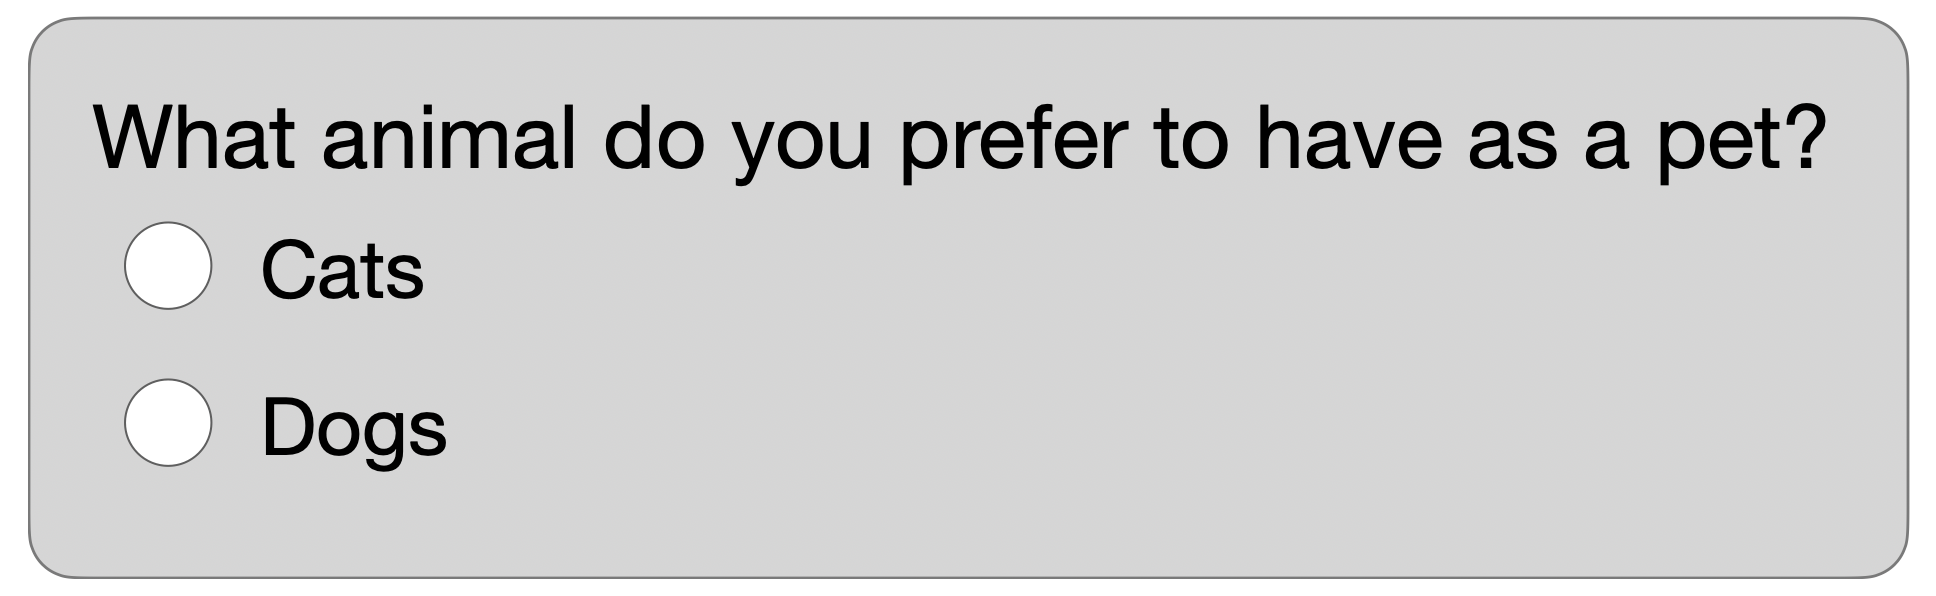
\includegraphics[width=0.7\linewidth]{images/PetExample1} 

}

\caption{Example Question Asking Pet Preference Type}\label{fig:overview-pet-examp1}
\end{figure}

This question may have validity issues as it only provides the options of ``dogs'' and ``cats'' to respondents, and the interpretation of the data could be incorrect. For example, if we had 100 respondents who answered the question and 50 selected dogs, then the results of this question cannot be ``50\% of the population prefers to have a dog as a pet,'' as only two response options were provided. If a respondent taking our survey prefers turtles, they could either be forced to choose a response between these two (i.e., interpret the question as ``between dogs and cats, which do you prefer?'' and result in \emph{measurement error}), or they may not answer the question (which results in \emph{item nonresponse error}). Based on this, the interpretation of this question should be, ``When given a choice between dogs and cats, 50\% of respondents preferred to have a dog as a pet.''

To avoid this issue, researchers should consider these possibilities and adjust the question accordingly. One simple way could be to add an ``other'' response option to give respondents a chance to provide a different response. The ``other'' response option could then include a way for respondents to write their other preference. For example, we could rewrite this question as:

\begin{figure}

{\centering 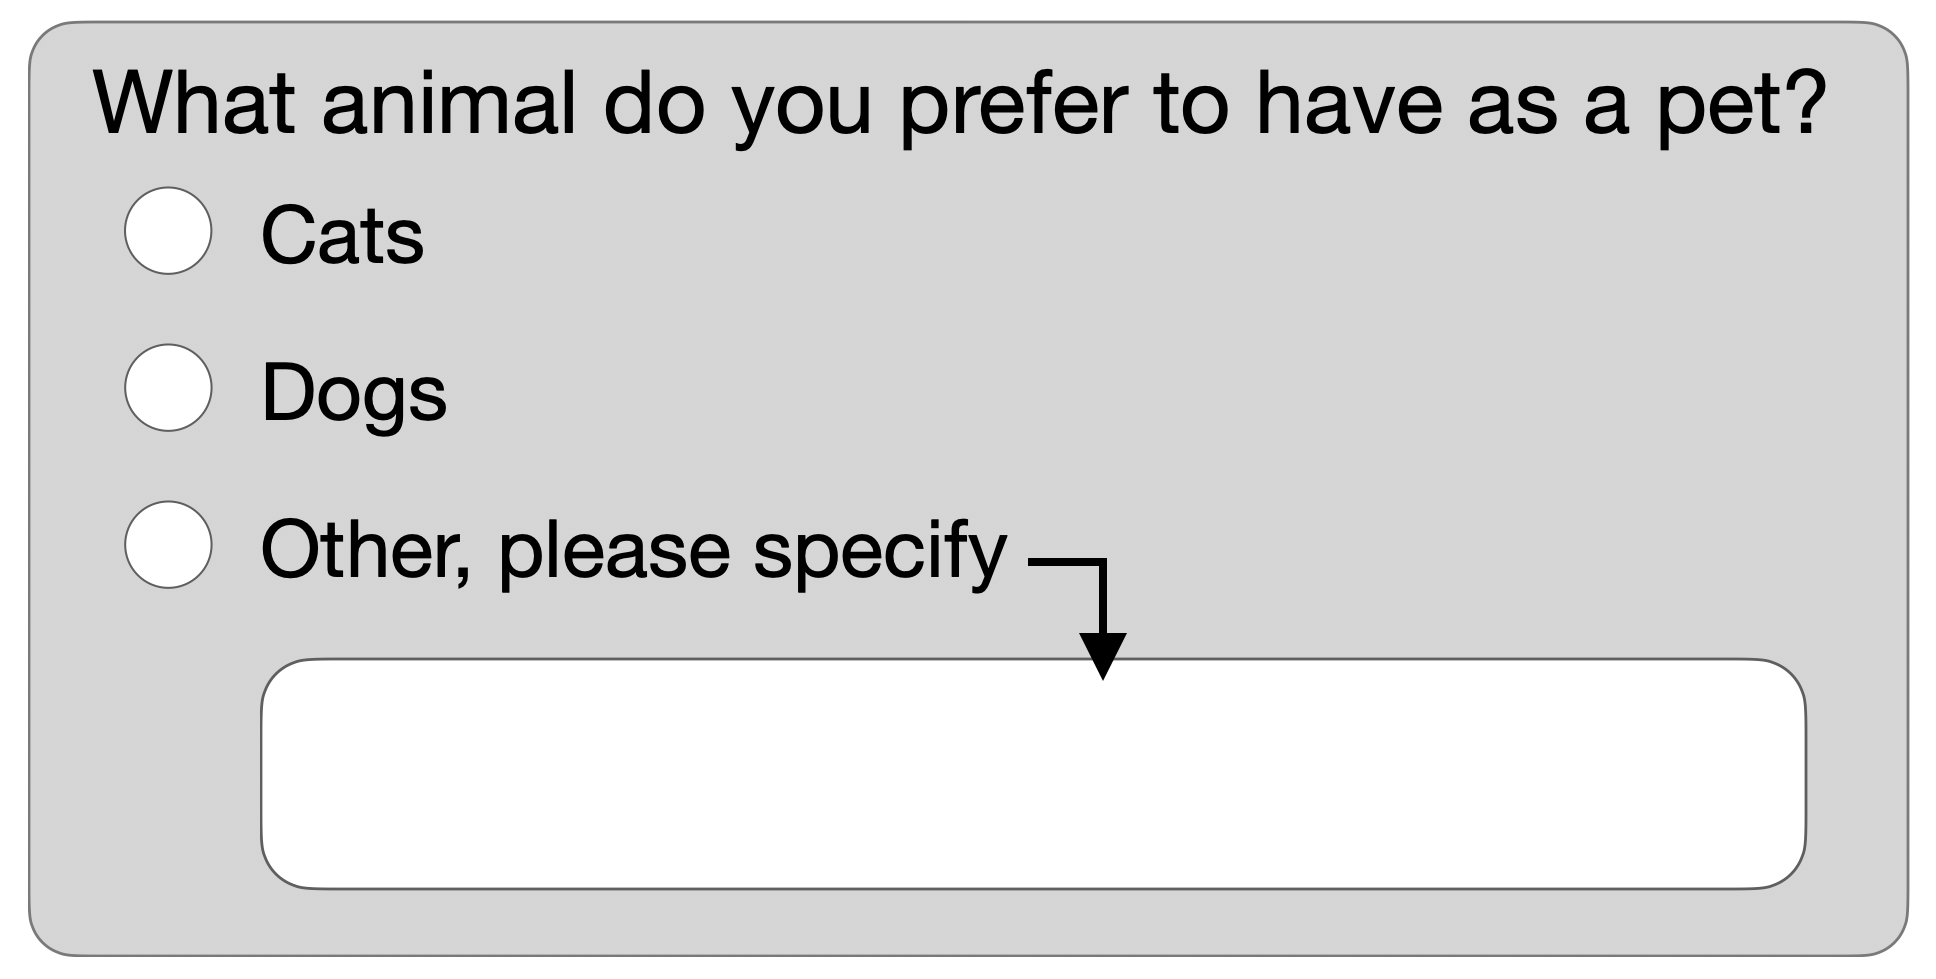
\includegraphics[width=0.7\linewidth]{images/PetExample2} 

}

\caption{Example Question Asking Pet Preference Type with Other Specify Option}\label{fig:overview-pet-examp2}
\end{figure}

Researchers can then code the responses from the open-ended box and get a better understanding of the respondent's choice of preferred pet. Interpreting this question becomes easier as researchers no longer need to qualify the results with the choices provided.

This is a simple example of how the presentation of the question and options can impact the findings. For more complex topics and questions, researchers must thoroughly consider how to mitigate any impacts from the presentation, formatting, wording, and other aspects. As survey analysts, reviewing not only the data but also the wording of the questions is crucial to ensure the results are presented in a manner consistent with the question asked. Chapter \ref{c03-understanding-survey-data-documentation} provides further details on how to review existing survey documentation to inform our analyses.

\hypertarget{overview-datacollection}{%
\section{Data Collection}\label{overview-datacollection}}

Once the data collection starts, researchers try to stick to the data collection protocol designed during pre-survey planning. However, effective researchers also prepare to adjust their plans and adapt as needed to the current progress of data collection \citep{Schouten2018}. Some extreme examples could be natural disasters that could prevent mailings or interviewers getting to the sample members. This could cause an in-person survey needing to quickly pivot to a self-administered survey, or the field period could be delayed, for example. Others could be smaller in that something newsworthy occurs connected to the survey, so researchers could choose to play this up in communication materials. In addition to these external factors, there could be factors unique to the survey, such as lower response rates for a specific sub-group, so the data collection protocol may need to find ways to improve response rates for that specific group.

\hypertarget{overview-post}{%
\section{Post-Survey Processing}\label{overview-post}}

After data collection, various activities need to be completed before we can analyze the survey. Multiple decisions made during this post-survey phase can assist researchers in reducing different error sources, such as weighting to account for the sample selection. Knowing the decisions researchers made in creating the final analytic data can impact how analysts use the data and interpret the results.

\hypertarget{overview-post-cleaning}{%
\subsection{Data Cleaning and Imputation}\label{overview-post-cleaning}}

Post-survey cleaning is one of the first steps researchers do to get the survey responses into a dataset for use by analysts. Data cleaning can consist of correcting inconsistent data (e.g., with skip pattern errors or multiple questions throughout the survey being consistent with each other), editing numeric entries or open-ended responses for grammar and consistency, or recoding open-ended questions into categories for analysis. There is no universal set of fixed rules that every project must adhere to. Instead, each project or research study should establish its own guidelines and procedures for handling various cleaning scenarios based on its specific objectives.

Researchers should use their best judgment to ensure data integrity, and all decisions should be documented and available to those using the data in the analysis. Each decision a researcher makes impacts \emph{processing error}, so often, researchers have multiple people review these rules or recode open-ended data and adjudicate any differences in an attempt to reduce this error.

Another crucial step in post-survey processing is \emph{imputation}. Often, there is item nonresponse where respondents do not answer specific questions. If the questions are crucial to analysis efforts or the research question, researchers may implement imputation to reduce \emph{item nonresponse error}. Imputation is a technique for replacing missing or incomplete data values with estimated values. However, as imputation is a way of assigning a value to missing data based on an algorithm or model, it can also introduce \emph{processing error}, so researchers should consider the overall implications of imputing data compared to having item nonresponse. There are multiple ways to impute data. We recommend reviewing other resources like \citet{Kim2021} for more information.

\hypertarget{overview-post-cleaning-ex}{%
\subsubsection*{Example: Number of Pets in a Household}\label{overview-post-cleaning-ex}}


Let's return to the question we created to ask about \protect\hyperlink{overview-design-questionnaire-ex}{animal preference}. The ``other specify'' invites respondents to specify the type of animal they prefer to have as a pet. If respondents entered answers such as ``puppy,'' ``turtle,'' ``rabit,'' ``rabbit,'' ``bunny,'' ``ant farm,'' ``snake,'' ``Mr.~Purr,'' then researchers may wish to categorize these write-in responses to help with analysis. In this example, ``puppy'' could be assumed to be a reference to a ``Dog'', and could be recoded there. The misspelling of ``rabit'' could be coded along with ``rabbit'' and ``bunny'' into a single category of ``Bunny or Rabbit''. These are relatively standard decisions that a researcher could make. The remaining write-in responses could be categorized in a few different ways. ``Mr.~Purr,'' which may be someone's reference to their own cat, could be recoded as ``Cat'', or it could remain as ``Other'' or some category that is ``Unknown''. Depending on the number of responses related to each of the others, they could all be combined into a single ``Other'' category, or maybe categories such as ``Reptiles'' or ``Insects'' could be created. Each of these decisions may impact the interpretation of the data, so our researchers should document the types of responses that fall into each of the new categories and any decisions made.

\hypertarget{overview-post-weighting}{%
\subsection{Weighting}\label{overview-post-weighting}}

We can address some of the error sources identified in the previous sections using \emph{weighting}. During the weighting process, weights are created for each respondent record. These weights allow the survey responses to generalize to the population. A weight, generally, reflects how many units in the population each respondent represents, and, often the weight is constructed such that the sum of the weights is the size of the population.

Weights can address coverage, sampling, and nonresponse errors. Many published surveys include an ``analysis weight'' variable that combines these adjustments. However, weighting itself can also introduce \emph{adjustment error}, so researchers need to balance which types of errors should be corrected with weighting. The construction of weights is outside the scope of this book, and researchers should reference other materials if interested in constructing their own \citep{Valliant2018weights}. Instead, this book assumes the survey has been completed, weights are constructed, and data is available to users.

\hypertarget{overview-post-weighting-ex}{%
\subsubsection*{Example: Number of Pets in a Household}\label{overview-post-weighting-ex}}


In the simple example of our survey, we decided to obtain a random sample from each state to select our sample members. Knowing this sampling design, our researcher can include selection weights for analysis that account for how the sample members were selected for the survey. Additionally, the sampling frame may have the type of building associated with each address, so we could include the building type as a potential nonresponse weighting variable, along with some interviewer observations that may be related to our research topic of the average number of pets in a household. Combining these weights, we can create an analytic weight that researchers need to use when analyzing the data.

\hypertarget{overview-post-disclosure}{%
\subsection{Disclosure}\label{overview-post-disclosure}}

Before data is released publicly, researchers need to ensure that individual respondents can not be identified by the data when confidentiality is required. There are a variety of different methods that can be used. Here we describe a few of the most commonly used:

\begin{itemize}
\tightlist
\item
  \textbf{Data swapping}: Researchers may swap specific data values across different respondents so that it does not impact insights from the data but ensures that specific individuals cannot be identified.
\item
  \textbf{Top/bottom coding}: Researchers may choose top or bottom coding to mask extreme values. For example, researchers may top-code income values such that households with income greater than \$500,000 are coded as ``\$500,000 or more'' with other incomes being presented as integers between \$0 and \$499,999. This can impact analyses at the tails of the distribution.
\item
  \textbf{Coarsening}: Researchers may use coarsening to mask unique values. For example, a survey question may ask for a precise income but the public data may include data as a categorical variable. Another example commonly used in survey practice is to coarsen geographic variables. Data collectors likely know the precise address of sample members but the public data may only include the state or even region of respondents.
\item
  \textbf{Perturbation}: Researchers may add random noise to outcomes. As with swapping, this is done so that it does not impact insights from the data but ensures that specific individuals cannot be identified.
\end{itemize}

There is as much art as there is science to the methods used for disclosure. In the survey documentation, researchers will only provide high-level comments about the disclosure and not specific details. This ensures nobody can reverse the disclosure and thus identify individuals. For more information on different disclosure methods, please see \citet{Skinner2009} and the \href{https://www-archive.aapor.org/Standards-Ethics/AAPOR-Code-of-Ethics/Survey-Disclosure-Checklist.aspx}{AAPOR Standards}.

\hypertarget{overview-post-documentation}{%
\subsection{Documentation}\label{overview-post-documentation}}

Documentation is a critical step of the survey life cycle. Researchers systematically record all the details, decisions, procedures, and methodologies to ensure transparency, reproducibility, and the overall quality of survey research.

Proper documentation allows analysts to understand, reproduce, and evaluate the study's methods and findings. Chapter \ref{c03-understanding-survey-data-documentation} dives into how analysts should use survey data documentation.

\hypertarget{post-survey-data-analysis-and-reporting}{%
\section{Post-survey data analysis and reporting}\label{post-survey-data-analysis-and-reporting}}

After completing the survey life cycle, the data is ready for analysts to use. The rest of this book continues from this point. For more information on the survey life cycle, please explore the references cited throughout this chapter.

\hypertarget{c03-understanding-survey-data-documentation}{%
\chapter{Understanding Survey Data Documentation}\label{c03-understanding-survey-data-documentation}}

\hypertarget{introduction-1}{%
\section{Introduction}\label{introduction-1}}

Survey documentation helps us prepare before we look at the actual survey data. The documentation includes technical guides, questionnaires, codebooks, errata, and other useful resources. By taking the time to review these materials, we can gain a comprehensive understanding of the survey data (including research and design decisions discussed in Chapters \ref{c02-overview-surveys} and \ref{c10-specifying-sample-designs}) and conduct our analysis more effectively.

Survey documentation can vary in organization, type, and ease of use. The information may be stored in any format - PDFs, Excel spreadsheets, Word documents, and so on. Some surveys bundle documentation together, such as providing the codebook and questionnaire in a single document. Others keep them in separate files. Despite these variations, we can gain a general understanding of the documentation types and what aspects to focus on in each.

\hypertarget{types-of-survey-documentation}{%
\section{Types of survey documentation}\label{types-of-survey-documentation}}

\hypertarget{technical-documentation}{%
\subsection{Technical documentation}\label{technical-documentation}}

The technical documentation, also known as user guides or methodology/analysis guides, highlights the variables necessary to specify the survey design. We recommend concentrating on these key sections:

\begin{itemize}
\tightlist
\item
  \textbf{Introduction:} The introduction orients us to the survey. This section provides the project's background, the study's purpose, and the main research questions.
\item
  \textbf{Study design:} The study design section describes how researchers prepared and administered the survey.
\item
  \textbf{Sample:} The sample section describes the sample frame, any known sampling errors, and the limitations of the sample. This section can contain recommendations on how to use sampling weights. Look for weight information, whether the survey design contains strata, clusters/PSUs, or replicate weights. Also look for population sizes, finite population correction, or replicate weight scaling information. Additional detail on sample designs is available in Chapter \ref{c10-specifying-sample-designs}.
\item
  \textbf{Notes on fielding:} Any additional notes on fielding, such as response rates, may be found in the technical documentation.
\end{itemize}

The technical documentation may include other helpful resources. Some technical documentation includes syntax for SAS, SUDAAN, Stata, and/or R, so we do not have to create this code from scratch.

\hypertarget{questionnaires}{%
\subsection{Questionnaires}\label{questionnaires}}

A questionnaire is a series of questions used to collect information from people in a survey. It can ask about opinions, behaviors, demographics, or even just numbers like the count of lightbulbs, square footage, or farm size. Questionnaires can employ different types of questions, such as closed-ended (e.g., select one or check all that apply), open-ended (e.g., numeric or text), Likert scales (e.g., a 5- or 7-point scale specifying a respondent's level of agreement to a statement), or ranking questions (e.g., a list of options that a respondent ranks by preference). It may randomize the display order of responses or include instructions that help respondents understand the questions. A survey may have one questionnaire or multiple, depending on its scale and scope.

The questionnaire is another important resource for understanding and interpreting the survey data (see Section \ref{overview-design-questionnaire}), and we should use it alongside any analysis. It provides details about each of the questions asked in the survey, such as question name, question wording, response options, skip logic, randomizations, display specification, mode differences, and the universe (the subset of respondents that were asked a question).

Below, in Figure \ref{fig:understand-que-examp}, we show an example from the ANES 2020 questionnaire \citep{anes-svy}. The figure shows a question's question name (\texttt{POSTVOTE\_RVOTE}), description (Did R Vote?), full wording of the question and responses, response order, universe, question logic (this question was only asked if \texttt{vote\_pre} = 0), and other specifications. The section also includes the variable name, which we can link to the codebook.

\begin{figure}
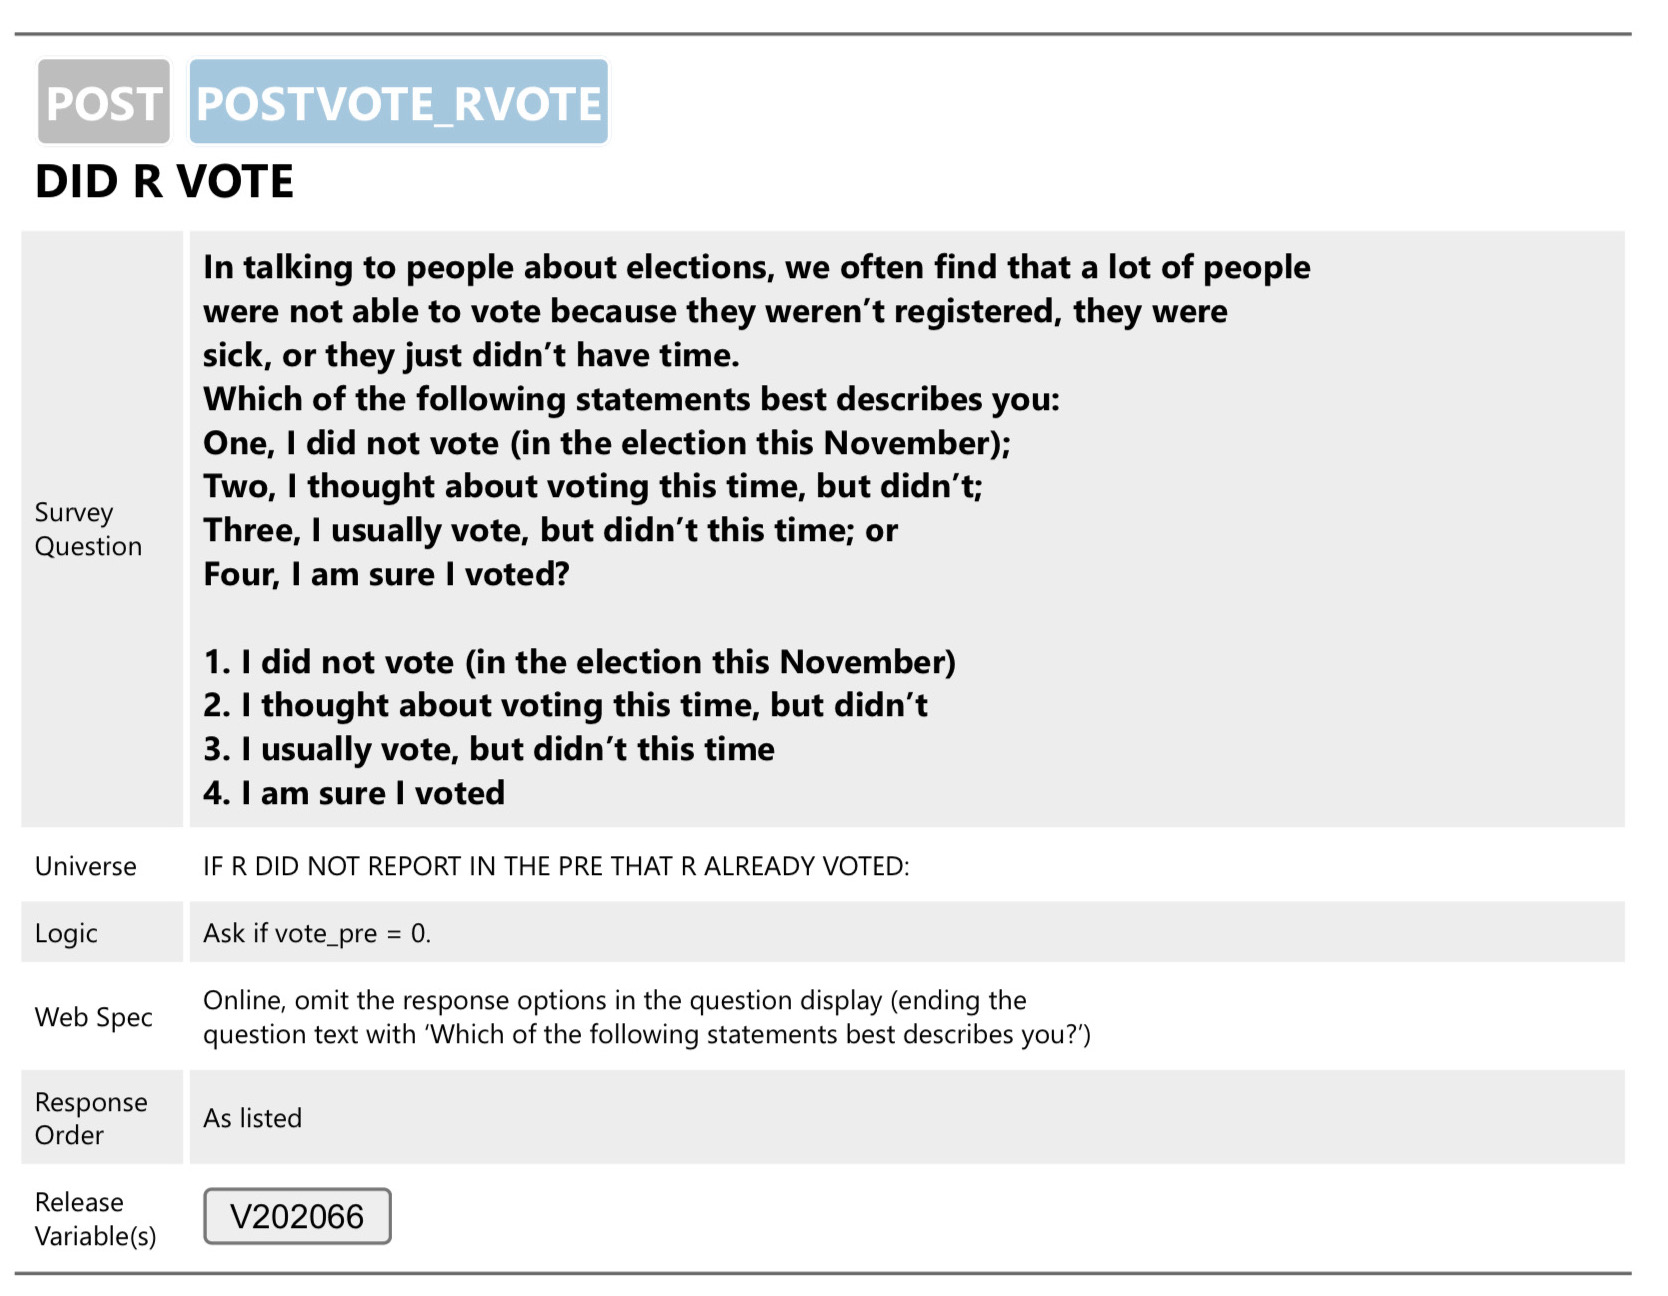
\includegraphics{images/questionnaire-example} \caption{ANES 2020 Questionnaire Example}\label{fig:understand-que-examp}
\end{figure}

The content and structure of questionnaires vary depending on the specific survey. For instance, question names may be informative (like the ANES example above), sequential, or denoted by a code. In some cases, surveys may not use separate names for questions and variables. Figure \ref{fig:understand-que-examp-2} shows an example from the Behavioral Risk Factor Surveillance System (BRFSS) questionnaire that shows a sequential question number and a coded variable name (as opposed to a question name) \citep{brfss-svy}.

\begin{figure}
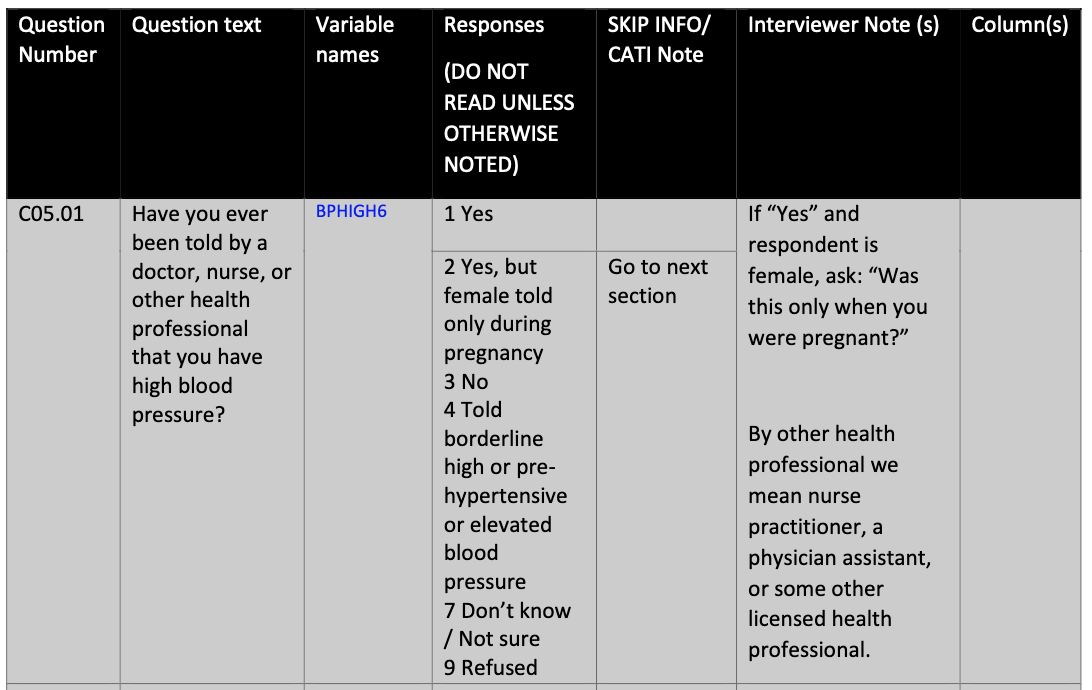
\includegraphics{images/questionnaire-example-2} \caption{BRFSS 2021 Questionnaire Example}\label{fig:understand-que-examp-2}
\end{figure}

We should factor in the details of a survey when conducting our analyses. For example, surveys that use various modes (e.g., web and mail) may have differences in question wording or skip logic, as web surveys can include fills or automate skip logic. These variations could warrant separate analyses for each mode.

\hypertarget{codebooks}{%
\subsection{Codebooks}\label{codebooks}}

While a questionnaire provides information about the questions posed to respondents, the codebook explains how the survey data was coded and recorded. It lists details such as variable names, variable labels, variable meanings, codes for missing data, value labels, and value types (whether categorical or continuous, etc.). The codebook helps us understand and use the variables appropriately in our analysis. In particular, the codebook (as opposed to the questionnaire) often includes information on missing data. Note that the term \emph{data dictionary} is sometimes used interchangeably with codebook, but a data dictionary may include more details on the structure and elements of the data.

Figure \ref{fig:understand-codebook-examp} is a question from the ANES 2020 codebook \citep{anes-cb}. This section indicates a particular variable's name (\texttt{V202066}), question wording, value labels, universe, and associated survey question (\texttt{POSTVOTE\_RVOTE}).

\begin{figure}
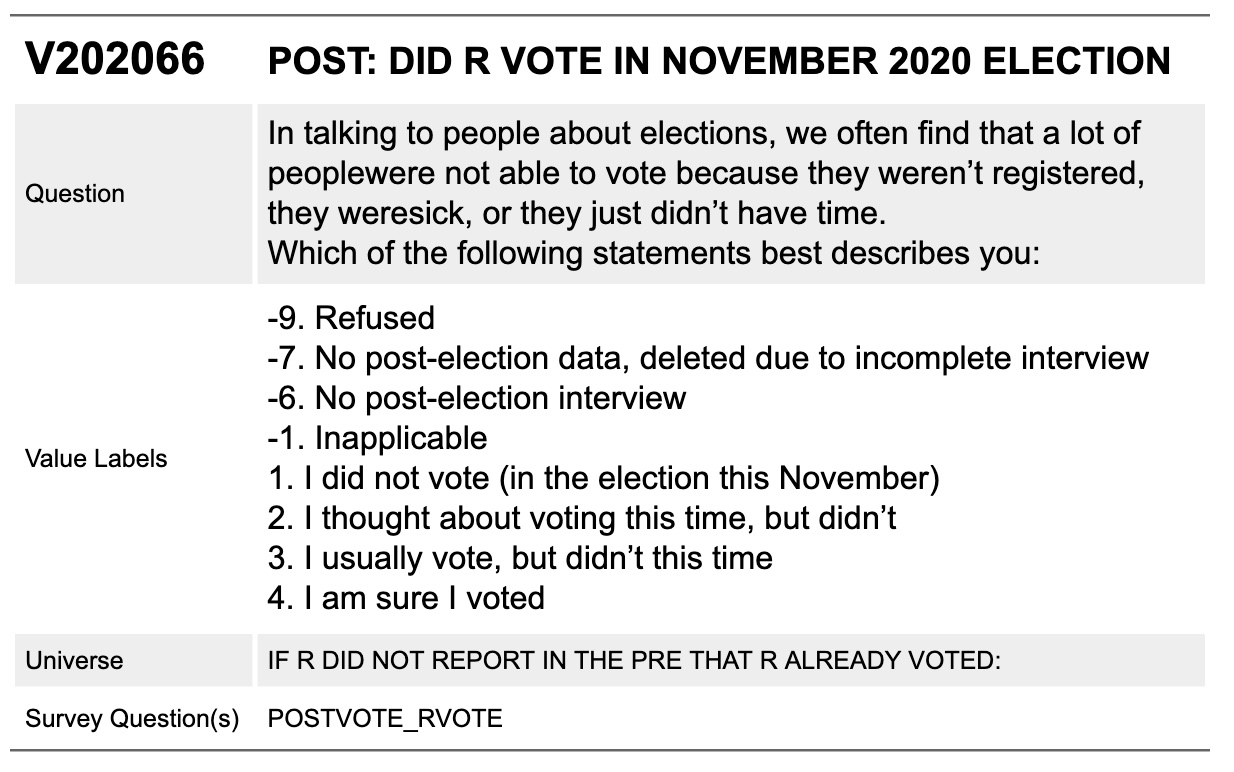
\includegraphics{images/codebook-example} \caption{ANES 2020 Codebook Example}\label{fig:understand-codebook-examp}
\end{figure}

Reviewing the questionnaires and codebooks in parallel can clarify how to interpret the variables (Figures \ref{fig:understand-que-examp} and \ref{fig:understand-codebook-examp}), as questions and variables do not always correspond directly to each other in a one-to-one mapping. A single question may have multiple associated variables, or a single variable may summarize multiple questions.

\hypertarget{errata}{%
\subsection{Errata}\label{errata}}

An erratum (singular) or errata (plural) is a document that lists errors found in a publication or dataset. The purpose of an erratum is to correct or update inaccuracies in the original document. Examples of errata include:

\begin{itemize}
\tightlist
\item
  Issuing a corrected data table after realizing a typo or mistake in a table cell
\item
  Reporting incorrectly programmed skips in an electronic survey where questions are skipped by the respondent when they should not have been
\end{itemize}

The 2004 ANES dataset released an erratum, notifying analysts to remove a specific row from the data file due to the inclusion of a respondent who should not have been part of the sample. Adhering to an issued erratum helps us increase the accuracy and reliability of analysis.

\hypertarget{additional-resources}{%
\subsection{Additional resources}\label{additional-resources}}

Survey documentation may include additional material, such as interviewer instructions or ``show cards'' provided to respondents during interviewer-administered surveys to help respondents answer questions. Explore the survey website to find out what resources were used and in what contexts.

\hypertarget{missing-data-coding}{%
\section{Missing data coding}\label{missing-data-coding}}

For some observations in a dataset, there may be missing data. This can be by design or from nonresponse, and these concepts are detailed in Chapter \ref{c11-missing-data}. In that chapter, we also discuss how to analyze data with missing data. In this section, we discuss how to understand documentation related to missing data.

The survey documentation, often the codebook, represents the missing data with a code. The codebook may list different codes depending on why certain data is missing. In the example of variable \texttt{V202066} from the ANES (Figure \ref{fig:understand-codebook-examp}), \texttt{-9} represents ``Refused,'' \texttt{-7} means that the response was deleted due to an incomplete interview, \texttt{-6} means that there is no response because there was no follow-up interview, and \texttt{-1} means ``Inapplicable'' (due to the designed skip pattern).

As another example, there may be a summary variable that describes the missingness of a set of variables - particularly with ``select all that apply'' or ``multiple response'' questions. In the National Crime Victimization Survey (NCVS), respondents who are victims of a crime and saw the offender are asked if the offender have a weapon and then asked what the type of weapon was. This part of the questionnaire from 2021 is shown in Figure \ref{fig:understand-ncvs-weapon-q}.

\begin{figure}
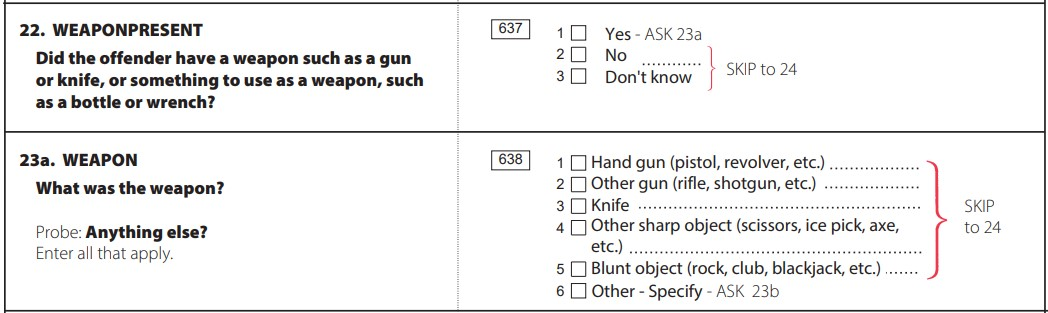
\includegraphics{images/questionnaire-ncvs-weapon} \caption{Excerpt from the NCVS 2020-2021 Crime Incident Report - Weapon Type}\label{fig:understand-ncvs-weapon-q}
\end{figure}

The NCVS codebook includes coding for all multiple response variables of a ``lead in'' variable that summarizes the individual options. For question 23a on the weapon type, the lead in variable is V4050 which is shown in \ref{fig:understand-ncvs-weapon-cb}. This variable is then followed by a set of variables for each weapon type. An example of one of the individual variables from the codebook, the handgun, is shown in \ref{fig:understand-ncvs-weapon-cb-hg}. We will dive in more to this example in Chapter \ref{c11-missing-data} of how to analyze this variable.

\begin{figure}
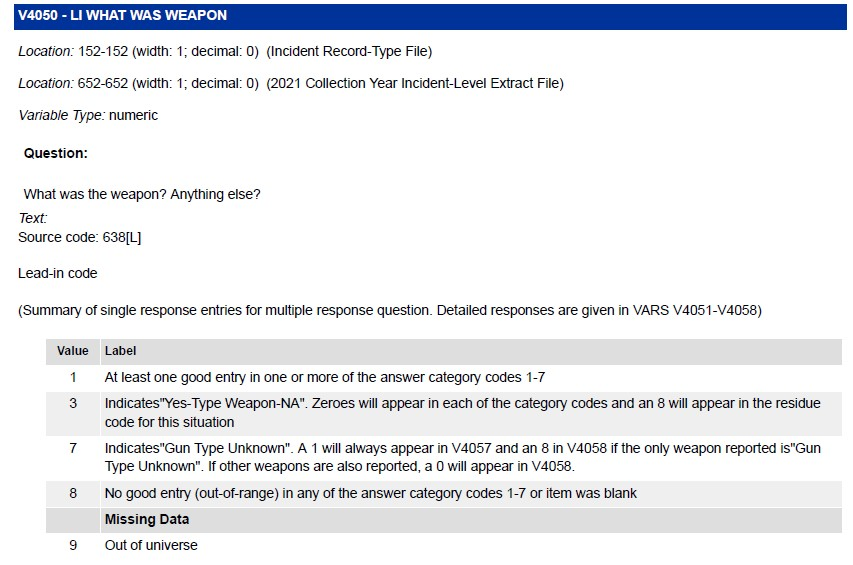
\includegraphics{images/codebook-ncvs-weapon-li} \caption{Excerpt from the NCVS 2021 Codebook for V4050 - LI WHAT WAS WEAPON}\label{fig:understand-ncvs-weapon-cb}
\end{figure}

\begin{figure}
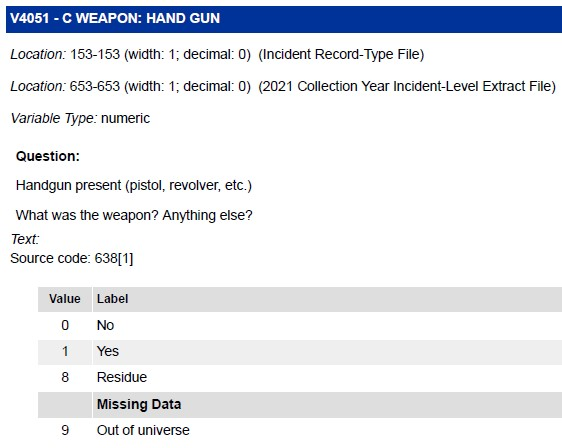
\includegraphics{images/codebook-ncvs-weapon-handgun} \caption{Excerpt from the NCVS 2021 Codebook for V4051 - C WEAPON: HAND GUN}\label{fig:understand-ncvs-weapon-cb-hg}
\end{figure}

When data is read into R, some values may be system missing, that is they are coded as \texttt{NA} even if that is not evident in a codebook. We will discuss in Chapter \ref{c11-missing-data} how to analyze data with \texttt{NA} values and review how R handles missing data in calculations.

\hypertarget{example-american-national-election-studies-anes-2020-survey-documentation}{%
\section{Example: American National Election Studies (ANES) 2020 Survey Documentation}\label{example-american-national-election-studies-anes-2020-survey-documentation}}

Let's look at the survey documentation for the American National Election Studies (ANES) 2020. The survey website is located at \url{https://electionstudies.org/data-center/2020-time-series-study/}.

Navigating to ``User Guide and Codebook'' \citep{anes-cb}, we can download the PDF that contains the survey documentation, titled ``ANES 2020 Time Series Study Full Release: User Guide and Codebook''. Do not be daunted by the 796-page PDF. We will focus on the most critical information.

\hypertarget{introduction-2}{%
\subsubsection*{Introduction}\label{introduction-2}}


The first section in the User Guide explains that the ANES 2020 Times Series Study continues a series of election surveys conducted since 1948. These surveys contain data on public opinion and voting behavior in the U.S. presidential elections. The introduction also includes information about the modes used for data collection (web, live video interviewing, or CATI). Additionally, there is a summary of the number of pre-election interviews (8,280) and post-election re-interviews (7,449).

\hypertarget{sample-design-and-respondent-recruitment}{%
\subsubsection*{Sample Design and Respondent Recruitment}\label{sample-design-and-respondent-recruitment}}


The section ``Sample Design and Respondent Recruitment'' provides more detail about the survey's sequential mixed-mode design. All three modes were conducted one after another and not at the same time. Additionally, it indicates that for the 2020 survey, they resampled all respondents who participated in 2016 ANES, along with a newly-drawn cross-section:

\begin{quote}
The target population for the fresh cross-section was the 231 million non-institutional U.S. citizens aged 18 or older living in the 50 U.S. states or the District of Columbia.
\end{quote}

The document continues with more details on the sample groups.

\hypertarget{data-analysis-weights-and-variance-estimation}{%
\subsubsection*{Data Analysis, Weights, and Variance Estimation}\label{data-analysis-weights-and-variance-estimation}}


The section ``Data Analysis, Weights, and Variance Estimation'' includes information on weights and strata/cluster variables. Reading through, we can find the full sample weight variables:

\begin{quote}
For analysis of the complete set of cases using pre-election data only, including all cases and representative of the 2020 electorate, use the full sample pre-election weight, \textbf{V200010a}. For analysis including post-election data for the complete set of participants (i.e., analysis of post-election data only or a combination of pre- and post-election data), use the full sample post-election weight, \textbf{V200010b}. Additional weights are provided for analysis of subsets of the data\ldots{}
\end{quote}

The document provides more information about the variables, summarized in Table \ref{tab:aneswgts}.

\begin{longtable}[]{@{}ccc@{}}
\caption{\label{tab:aneswgts} Weight and variance information for ANES}\tabularnewline
\toprule\noalign{}
For weight & Use variance unit/PSU/cluster & and use variance stratum \\
\midrule\noalign{}
\endfirsthead
\toprule\noalign{}
For weight & Use variance unit/PSU/cluster & and use variance stratum \\
\midrule\noalign{}
\endhead
\bottomrule\noalign{}
\endlastfoot
V200010a & V200010c & V200010d \\
V200010b & V200010c & V200010d \\
\end{longtable}

\hypertarget{methodology}{%
\subsection*{Methodology}\label{methodology}}


The user guide mentions a supplemental document called ``How to Analyze ANES Survey Data'' \citep{debell} as a `how-to guide' for analyzing the data. In this document, we learn more about the weights, where we learn that they sum to the sample size and not the population. If our goal is to calculate estimates for the entire U.S. population instead of just the sample, we must adjust the weights to the U.S. population. To create accurate weights for the population, we need to determine the total population size at the time of the survey. Let's review the ``Sample Design and Respondent Recruitment'' section for more details:

\begin{quote}
The target population for the fresh cross-section was the 231 million non-institutional U.S. citizens aged 18 or older living in the 50 U.S. states or the District of Columbia.
\end{quote}

The documentation suggests that the population should equal around 231 million, but this is a very imprecise count. Upon further investigation in the available resources, we can find the methodology file titled ``Methodology Report for the ANES 2020 Time Series Study'' \citep{anes-2020-tech}. This file states that we can use the population total from the Current Population Survey (CPS), a monthly survey sponsored by the U.S. Census Bureau and the U.S. Bureau of Labor Statistics. The CPS provides a more accurate population estimate for a specific month. Therefore, we can use the CPS to get the total population number for March 2020, the time in which the ANES was conducted. Chapter \ref{c04-getting-started} goes into detailed instructions on how to calculate and adjust this value in the data.

\hypertarget{part-analysis}{%
\part{Analysis}\label{part-analysis}}

\hypertarget{c04-getting-started}{%
\chapter{Getting started}\label{c04-getting-started}}

\hypertarget{introduction-3}{%
\section{Introduction}\label{introduction-3}}

This chapter provides an overview of the packages, data, and design objects we use frequently throughout this book. As mentioned in Chapter \ref{c02-overview-surveys}, understanding how a survey was conducted helps us make sense of the results and interpret findings. Therefore, we provide background on the datasets used in examples and exercises. Next, we walk through how to create the survey design objects necessary to begin analysis. Finally, we provide an overview of the \{srvyr\} package and the steps needed for analysis. If you have questions or face issues while going through the book, please report them in the book's \href{https://github.com/tidy-survey-r/tidy-survey-book}{GitHub repository}.

\hypertarget{setup}{%
\section{Setup}\label{setup}}

The Setup section provides details on the required packages and data, as well as the steps for preparing survey design objects. For a streamlined learning experience, we recommend taking the time to walk through the code provided and making sure everything is properly set up.

\hypertarget{packages}{%
\subsection{Packages}\label{packages}}

We use several packages throughout the book, but let's install and load specific ones for this chapter. Many functions in the examples and exercises are from three packages: \{tidyverse\}, \{survey\}, and \{srvyr\}. If they are not already installed, use the code below. The \{tidyverse\} and \{survey\} packages can both be installed from the Comprehensive R Archive Network (CRAN). We use the GitHub development version of \{srvyr\} because of its additional functionality compared to the one on CRAN. Install the package directly from GitHub using the \{remotes\} package:

\begin{Shaded}
\begin{Highlighting}[]
\FunctionTok{install.packages}\NormalTok{(}\FunctionTok{c}\NormalTok{(}\StringTok{"tidyverse"}\NormalTok{, }\StringTok{"survey"}\NormalTok{, }\StringTok{"remotes"}\NormalTok{))}
\NormalTok{remotes}\SpecialCharTok{::}\FunctionTok{install\_github}\NormalTok{(}\StringTok{"gergness/srvyr"}\NormalTok{)}
\end{Highlighting}
\end{Shaded}

We bundled the datasets used in the book in an R package, \{srvyrexploR\}. Install it directly from GitHub using the \{remotes\} package:

\begin{Shaded}
\begin{Highlighting}[]
\NormalTok{remotes}\SpecialCharTok{::}\FunctionTok{install\_github}\NormalTok{(}\StringTok{"tidy{-}survey{-}r/srvyrexploR"}\NormalTok{)}
\end{Highlighting}
\end{Shaded}

After installing these packages, load them using the \texttt{library()} function:

\begin{Shaded}
\begin{Highlighting}[]
\FunctionTok{library}\NormalTok{(tidyverse)}
\FunctionTok{library}\NormalTok{(survey)}
\FunctionTok{library}\NormalTok{(srvyr)}
\FunctionTok{library}\NormalTok{(srvyrexploR)}
\end{Highlighting}
\end{Shaded}

The packages \{broom\}, \{gt\}, and \{gtsummary\} play a role in displaying output and creating formatted tables. Install them with the provided code\footnote{Note: \{broom\} is already included in the tidyverse, so no separate installation is required}:

\begin{Shaded}
\begin{Highlighting}[]
\FunctionTok{install.packages}\NormalTok{(}\FunctionTok{c}\NormalTok{(}\StringTok{"gt"}\NormalTok{, }\StringTok{"gtsummary"}\NormalTok{))}
\end{Highlighting}
\end{Shaded}

After installing these packages, load them using the \texttt{library()} function:

\begin{Shaded}
\begin{Highlighting}[]
\FunctionTok{library}\NormalTok{(broom)}
\FunctionTok{library}\NormalTok{(gt)}
\FunctionTok{library}\NormalTok{(gtsummary)}
\end{Highlighting}
\end{Shaded}

Install and load the \{censusapi\} package to access the Current Population Survey (CPS), which we use to ensure accurate weighting of a key dataset in the book. Run the code below to install \{censusapi\}:

\begin{Shaded}
\begin{Highlighting}[]
\FunctionTok{install.packages}\NormalTok{(}\StringTok{"censusapi"}\NormalTok{)}
\end{Highlighting}
\end{Shaded}

After installing this package, load it using the \texttt{library()} function:

\begin{Shaded}
\begin{Highlighting}[]
\FunctionTok{library}\NormalTok{(censusapi)}
\end{Highlighting}
\end{Shaded}

Note that the \{censusapi\} package requires a Census API key, available for free from the \href{https://api.census.gov/data/key_signup.html}{U.S. Census Bureau website} (refer to the package documentation for more information). We recommend storing the Census API key in our R environment instead of directly in the code. After obtaining the API key, save it in your R environment by running \texttt{Sys.setenv()}:

\begin{Shaded}
\begin{Highlighting}[]
\FunctionTok{Sys.setenv}\NormalTok{(}\AttributeTok{CENSUS\_KEY =} \StringTok{"YOUR\_API\_KEY\_HERE"}\NormalTok{)}
\end{Highlighting}
\end{Shaded}

Then, restart the R session. Once the Census API key is stored, we can retrieve it in our R code with \texttt{Sys.getenv("CENSUS\_KEY")}.

There are a few other packages used in the book in limited frequency. We list them in the Prerequisite boxes at the beginning of each chapter. As we work through the book, make sure to check the Prerequisite box and install any missing packages before proceeding.

\hypertarget{data}{%
\subsection{Data}\label{data}}

As mentioned above, the \{srvyrexploR\} package contains the datasets used in the book. Once installed and loaded, explore the documentation using the \texttt{help()} function. Read the descriptions of the datasets to understand what they contain:

\begin{Shaded}
\begin{Highlighting}[]
\FunctionTok{help}\NormalTok{(}\AttributeTok{package =} \StringTok{"srvyrexploR"}\NormalTok{)}
\end{Highlighting}
\end{Shaded}

This book uses two main datasets: the American National Election Studies \citep[ANES --][]{debell} and the Residential Energy Consumption Survey \citep[RECS --][]{recs-2020-tech}. We can load these datasets individually with the \texttt{data()} function by specifying the dataset name as an argument. In the code below, we load the \texttt{anes\_2020} and \texttt{recs\_2020} datasets into objects with their respective names:

\begin{Shaded}
\begin{Highlighting}[]
\FunctionTok{data}\NormalTok{(anes\_2020)}
\FunctionTok{data}\NormalTok{(recs\_2020)}
\end{Highlighting}
\end{Shaded}

\hypertarget{american-national-election-studies-anes-data}{%
\subsubsection*{American National Election Studies (ANES) Data}\label{american-national-election-studies-anes-data}}


The ANES is a study that collects data from election surveys dating back to 1948. These surveys contain information on public opinion and voting behavior in U.S. presidential elections and some midterm elections\footnote{In the United States, presidential elections are held in years divisible by four. In other even years, there are elections at the federal level for congress which are referred to as midterm elections as they occur at the middle of the term of a president.}. They cover topics such as party affiliation, voting choice, and level of trust in the government. The 2020 survey, the data we use in the book, was fielded online, through live video interviews, or via computer-assisted telephone interviews (CATI).

When working with new survey data, analysts should review the survey documentation (see Chapter \ref{c03-understanding-survey-data-documentation}) to understand the data collection methods. The original ANES data contains variables starting with \texttt{V20} \citep{debell}, so to assist with our analysis throughout the book, we created descriptive variable names. For example, the respondent's age is now in a variable called \texttt{Age}, and gender is in a variable called \texttt{Gender}. These descriptive variables are included in the \{srvyrexploR\} package, and Table \ref{tab:anes-view-tab} displays the list of these renamed variables. A complete overview of all variables can be found in the online Appendix (Appendix \ref{anes-cb}).



\begin{longtable}{l}
\caption{\label{tab:anes-view-tab}List of created variables in the ANES Data}\\
\toprule
Variable Name \\ 
\midrule
CaseID \\ 
InterviewMode \\ 
Weight \\ 
VarUnit \\ 
Stratum \\ 
CampaignInterest \\ 
EarlyVote2020 \\ 
VotedPres2016 \\ 
VotedPres2016\_selection \\ 
PartyID \\ 
TrustGovernment \\ 
TrustPeople \\ 
Age \\ 
AgeGroup \\ 
Education \\ 
RaceEth \\ 
Gender \\ 
Income \\ 
Income7 \\ 
VotedPres2020 \\ 
VotedPres2020\_selection \\ 
\bottomrule
\end{longtable}

Before beginning an analysis, it is useful to view the data to understand the available variables. The \texttt{dplyr::glimpse()} function produces a list of all variables, their types (e.g., function, double), and a few example values. Below, we remove variables containing a ``V'' followed by numbers with \texttt{select(-matches("\^{}V\textbackslash{}\textbackslash{}d"))} before using \texttt{glimpse()} to get a quick overview of the data with descriptive variable names:

\begin{Shaded}
\begin{Highlighting}[]
\NormalTok{anes\_2020 }\SpecialCharTok{\%\textgreater{}\%}
  \FunctionTok{select}\NormalTok{(}\SpecialCharTok{{-}}\FunctionTok{matches}\NormalTok{(}\StringTok{"\^{}V}\SpecialCharTok{\textbackslash{}\textbackslash{}}\StringTok{d"}\NormalTok{)) }\SpecialCharTok{\%\textgreater{}\%}
  \FunctionTok{glimpse}\NormalTok{()}
\end{Highlighting}
\end{Shaded}

\begin{verbatim}
## Rows: 7,453
## Columns: 21
## $ CaseID                  <dbl> 200015, 200022, 200039, 200046, 200053~
## $ InterviewMode           <fct> Web, Web, Web, Web, Web, Web, Web, Web~
## $ Weight                  <dbl> 1.0057, 1.1635, 0.7687, 0.5210, 0.9658~
## $ VarUnit                 <fct> 2, 2, 1, 2, 1, 2, 1, 2, 2, 2, 1, 1, 2,~
## $ Stratum                 <fct> 9, 26, 41, 29, 23, 37, 7, 37, 32, 41, ~
## $ CampaignInterest        <fct> Somewhat interested, Not much interest~
## $ EarlyVote2020           <fct> NA, NA, NA, NA, NA, NA, NA, NA, Yes, N~
## $ VotedPres2016           <fct> Yes, Yes, Yes, Yes, Yes, No, Yes, No, ~
## $ VotedPres2016_selection <fct> Trump, Other, Clinton, Clinton, Trump,~
## $ PartyID                 <fct> Strong republican, Independent, Indepe~
## $ TrustGovernment         <fct> Never, Never, Some of the time, About ~
## $ TrustPeople             <fct> About half the time, Some of the time,~
## $ Age                     <dbl> 46, 37, 40, 41, 72, 71, 37, 45, 70, 43~
## $ AgeGroup                <fct> 40-49, 30-39, 40-49, 40-49, 70 or olde~
## $ Education               <fct> Bachelor's, Post HS, High school, Post~
## $ RaceEth                 <fct> "Hispanic", "Asian, NH/PI", "White", "~
## $ Gender                  <fct> Male, Female, Female, Male, Male, Fema~
## $ Income                  <fct> "$175,000-249,999", "$70,000-74,999", ~
## $ Income7                 <fct> $125k or more, $60k to < 80k, $100k to~
## $ VotedPres2020           <fct> NA, Yes, Yes, Yes, Yes, Yes, Yes, NA, ~
## $ VotedPres2020_selection <fct> NA, Other, Biden, Biden, Trump, Biden,~
\end{verbatim}

From the output, we can see there are 7,453 rows and 21 variables in the ANES data. This output also indicates that most of the variables are factors (e.g., \texttt{InterviewMode}), while a few variables are in double (numeric) format (e.g., \texttt{Age}).

\hypertarget{residential-energy-consumption-survey-recs-data}{%
\subsubsection*{Residential Energy Consumption Survey (RECS) Data}\label{residential-energy-consumption-survey-recs-data}}


RECS is a study that measures energy consumption and expenditure in American households. Funded by the Energy Information Administration, the RECS data are collected through interviews with household members and energy suppliers. These interviews take place in person, over the phone, via mail, and on the web with modes changing over time. The survey has been fielded 14 times between 1950 and 2020. It includes questions about appliances, electronics, heating, air conditioning (A/C), temperatures, water heating, lighting, energy bills, respondent demographics, and energy assistance.

As mentioned above, analysts should read the survey documentation (see Chapter \ref{c03-understanding-survey-data-documentation}) to understand how the data was collected and implemented. Table \ref{tab:recs-view-tab} displays the list of variables in the RECS data (not including the weights, which start with \texttt{NWEIGHT} and will be described in more detail in Chapter \ref{c10-specifying-sample-designs}). An overview of all variables can be found in the online Appendix (Appendix \ref{recs-cb}).



\begin{longtable}{l}
\caption{\label{tab:recs-view-tab}List of Variables in the RECS Data}\\
\toprule
Variable Name \\ 
\midrule
DOEID \\ 
ClimateRegion\_BA \\ 
Urbanicity \\ 
Region \\ 
REGIONC \\ 
Division \\ 
STATE\_FIPS \\ 
state\_postal \\ 
state\_name \\ 
HDD65 \\ 
CDD65 \\ 
HDD30YR \\ 
CDD30YR \\ 
HousingUnitType \\ 
YearMade \\ 
TOTSQFT\_EN \\ 
TOTHSQFT \\ 
TOTCSQFT \\ 
ZTOTSQFT\_EN \\ 
ZYearMade \\ 
ZHousingUnitType \\ 
SpaceHeatingUsed \\ 
ZSpaceHeatingUsed \\ 
ACUsed \\ 
ZACUsed \\ 
ZACBehavior \\ 
HeatingBehavior \\ 
WinterTempDay \\ 
WinterTempAway \\ 
WinterTempNight \\ 
ACBehavior \\ 
SummerTempDay \\ 
SummerTempAway \\ 
SummerTempNight \\ 
ZHeatingBehavior \\ 
ZWinterTempAway \\ 
ZSummerTempAway \\ 
ZWinterTempDay \\ 
ZSummerTempDay \\ 
ZWinterTempNight \\ 
ZSummerTempNight \\ 
BTUEL \\ 
DOLLAREL \\ 
ZBTUEL \\ 
BTUNG \\ 
DOLLARNG \\ 
ZBTUNG \\ 
BTULP \\ 
DOLLARLP \\ 
ZBTULP \\ 
BTUFO \\ 
DOLLARFO \\ 
ZBTUFO \\ 
BTUWOOD \\ 
ZBTUWOOD \\ 
TOTALBTU \\ 
TOTALDOL \\ 
\bottomrule
\end{longtable}

Before starting an analysis, we recommend viewing the data to understand the types of data and variables that are included. The \texttt{dplyr::glimpse()} function produces a list of all variables, the type of the variable (e.g., function, double), and a few example values. Below, we remove the weight variables with \texttt{select(-matches("\^{}NWEIGHT"))} before using \texttt{glimpse()} to get a quick overview of the data:

\begin{Shaded}
\begin{Highlighting}[]
\NormalTok{recs\_2020 }\SpecialCharTok{\%\textgreater{}\%}
  \FunctionTok{select}\NormalTok{(}\SpecialCharTok{{-}}\FunctionTok{matches}\NormalTok{(}\StringTok{"\^{}NWEIGHT"}\NormalTok{)) }\SpecialCharTok{\%\textgreater{}\%}
  \FunctionTok{glimpse}\NormalTok{()}
\end{Highlighting}
\end{Shaded}

\begin{verbatim}
## Rows: 18,496
## Columns: 57
## $ DOEID             <dbl> 1e+05, 1e+05, 1e+05, 1e+05, 1e+05, 1e+05, 1e~
## $ ClimateRegion_BA  <fct> Mixed-Dry, Mixed-Humid, Mixed-Dry, Mixed-Hum~
## $ Urbanicity        <fct> Urban Area, Urban Area, Urban Area, Urban Ar~
## $ Region            <fct> West, South, West, South, Northeast, South, ~
## $ REGIONC           <chr> "WEST", "SOUTH", "WEST", "SOUTH", "NORTHEAST~
## $ Division          <fct> Mountain South, West South Central, Mountain~
## $ STATE_FIPS        <chr> "35", "05", "35", "45", "34", "48", "40", "2~
## $ state_postal      <fct> NM, AR, NM, SC, NJ, TX, OK, MS, DC, AZ, CA, ~
## $ state_name        <fct> New Mexico, Arkansas, New Mexico, South Caro~
## $ HDD65             <dbl> 3844, 3766, 3819, 2614, 4219, 901, 3148, 182~
## $ CDD65             <dbl> 1679, 1458, 1696, 1718, 1363, 3558, 2128, 23~
## $ HDD30YR           <dbl> 4451, 4429, 4500, 3229, 4896, 1150, 3564, 26~
## $ CDD30YR           <dbl> 1027, 1305, 1010, 1653, 1059, 3588, 2043, 21~
## $ HousingUnitType   <fct> Single-family detached, Apartment: 5 or more~
## $ YearMade          <ord> 1970-1979, 1980-1989, 1960-1969, 1980-1989, ~
## $ TOTSQFT_EN        <dbl> 2100, 590, 900, 2100, 800, 4520, 2100, 900, ~
## $ TOTHSQFT          <dbl> 2100, 590, 900, 2100, 800, 3010, 1200, 900, ~
## $ TOTCSQFT          <dbl> 2100, 590, 900, 2100, 800, 3010, 1200, 0, 50~
## $ ZTOTSQFT_EN       <fct> Not imputed, Not imputed, Not imputed, Not i~
## $ ZYearMade         <fct> Not imputed, Not imputed, Not imputed, Not i~
## $ ZHousingUnitType  <fct> Not imputed, Not imputed, Not imputed, Not i~
## $ SpaceHeatingUsed  <lgl> TRUE, TRUE, TRUE, TRUE, TRUE, TRUE, TRUE, TR~
## $ ZSpaceHeatingUsed <fct> Not imputed, Not imputed, Not imputed, Not i~
## $ ACUsed            <lgl> TRUE, TRUE, TRUE, TRUE, TRUE, TRUE, TRUE, FA~
## $ ZACUsed           <fct> Not imputed, Not imputed, Not imputed, Not i~
## $ ZACBehavior       <fct> Not imputed, Imputed, Not imputed, Not imput~
## $ HeatingBehavior   <fct> Set one temp and leave it, Turn on or off as~
## $ WinterTempDay     <dbl> 70, 70, 69, 68, 68, 76, 74, 70, 68, 70, 72, ~
## $ WinterTempAway    <dbl> 70, 65, 68, 68, 68, 76, 65, 70, 60, 70, 70, ~
## $ WinterTempNight   <dbl> 68, 65, 67, 68, 68, 68, 74, 68, 62, 68, 72, ~
## $ ACBehavior        <fct> Set one temp and leave it, Turn on or off as~
## $ SummerTempDay     <dbl> 71, 68, 70, 72, 72, 69, 68, NA, 72, 74, 77, ~
## $ SummerTempAway    <dbl> 71, 68, 68, 72, 72, 74, 70, NA, 76, 74, 77, ~
## $ SummerTempNight   <dbl> 71, 68, 68, 72, 72, 68, 70, NA, 68, 72, 77, ~
## $ ZHeatingBehavior  <fct> Not imputed, Not imputed, Not imputed, Not i~
## $ ZWinterTempAway   <fct> Not imputed, Not imputed, Not imputed, Not i~
## $ ZSummerTempAway   <fct> Not imputed, Not imputed, Not imputed, Not i~
## $ ZWinterTempDay    <fct> Not imputed, Not imputed, Not imputed, Not i~
## $ ZSummerTempDay    <fct> Not imputed, Not imputed, Not imputed, Not i~
## $ ZWinterTempNight  <fct> Not imputed, Not imputed, Not imputed, Not i~
## $ ZSummerTempNight  <fct> Not imputed, Not imputed, Not imputed, Not i~
## $ BTUEL             <dbl> 42723, 17889, 8147, 31647, 20027, 48968, 494~
## $ DOLLAREL          <dbl> 1955.06, 713.27, 334.51, 1424.86, 1087.00, 1~
## $ ZBTUEL            <fct> Not imputed, Not imputed, Imputed amount and~
## $ BTUNG             <dbl> 101924.4, 10145.3, 22603.1, 55118.7, 39099.5~
## $ DOLLARNG          <dbl> 701.83, 261.73, 188.14, 636.91, 376.04, 439.~
## $ ZBTUNG            <fct> Not imputed, Not imputed, Imputed, Not imput~
## $ BTULP             <dbl> 0, 0, 0, 0, 0, 0, 0, 0, 0, 0, 0, 0, 0, 0, 17~
## $ DOLLARLP          <dbl> 0.0, 0.0, 0.0, 0.0, 0.0, 0.0, 0.0, 0.0, 0.0,~
## $ ZBTULP            <fct> Not applicable, Not applicable, Not applicab~
## $ BTUFO             <dbl> 0, 0, 0, 0, 0, 0, 0, 0, 0, 0, 0, 0, 0, 0, 68~
## $ DOLLARFO          <dbl> 0, 0, 0, 0, 0, 0, 0, 0, 0, 0, 0, 0, 0, 0, 18~
## $ ZBTUFO            <fct> Not applicable, Not applicable, Not applicab~
## $ BTUWOOD           <dbl> 0, 0, 0, 0, 0, 3000, 0, 0, 0, 0, 0, 0, 0, 0,~
## $ ZBTUWOOD          <fct> Not applicable, Not applicable, Not applicab~
## $ TOTALBTU          <dbl> 144648, 28035, 30750, 86765, 59127, 85401, 1~
## $ TOTALDOL          <dbl> 2656.9, 975.0, 522.6, 2061.8, 1463.0, 2335.1~
\end{verbatim}

From the output, we can see that there are 18,496 rows and 57 non-weight variables in the RECS data. This output also indicates that most of the variables are in double (numeric) format (e.g., \texttt{TOTSQFT\_EN}), with some factor (e.g., \texttt{Region}), Boolean (e.g., \texttt{ACUsed}), character (e.g., \texttt{REGIONC}), and ordinal (e.g., \texttt{YearMade}) variables.

\hypertarget{setup-des-obj}{%
\subsection{Design objects}\label{setup-des-obj}}

The design object is the backbone for survey analysis. It is where we specify the sampling design, weights, and other necessary information to ensure we account for errors in the data. Before creating the design object, analysts should carefully review the survey documentation to understand how to create the design object for accurate analysis.

In this chapter, we provide details on how to code the design object for the ANES and RECS data used in the book. However, we only provide a high-level overview to get readers started. For a deeper understanding of creating these design objects for a variety of sampling designs, see Chapter \ref{c10-specifying-sample-designs}.

While we recommend conducting exploratory data analysis on the original data before diving into complex survey analysis (see Chapter \ref{c12-pitfalls}), the actual analysis and inference should be performed with the survey design objects instead of the original survey data. For example, the ANES data is called \texttt{anes\_2020}. If we create a survey design object called \texttt{anes\_des}, our analyses should begin with \texttt{anes\_des} and not \texttt{anes\_2020}. Using the survey design object ensures that our calculations are appropriately accounting for the details of the survey design.

\hypertarget{american-national-election-studies-anes-design-object}{%
\subsubsection*{American National Election Studies (ANES) Design Object}\label{american-national-election-studies-anes-design-object}}


The ANES documentation \citep{debell} details the sampling and weighting implications for analyzing the survey data. From this documentation and as noted in Chapter \ref{c03-understanding-survey-data-documentation}, the 2020 ANES data is weighted to the sample, not the population. To make generalizations about the population, we need to weigh the data against the full population count. The ANES methodology recommends using the Current Population Survey (CPS) to determine the number of non-institutional U.S. citizens aged 18 or older living in the 50 U.S. states or D.C. in March of 2020.

We can use the \{censusapi\} package to obtain the information needed for the survey design object. The \texttt{getCensus()} function allows us to retrieve the CPS data for March (\texttt{cps/basic/mar}) in 2020 (\texttt{vintage\ =\ 2020}). Additionally, we extract several variables from the CPS:

\begin{itemize}
\tightlist
\item
  month (\texttt{HRMONTH}) and year (\texttt{HRYEAR4}) of the interview: to confirm the correct time period
\item
  age (\texttt{PRTAGE}) of the respondent: to narrow the population to 18 and older (eligible age to vote)
\item
  citizenship status (\texttt{PRCITSHP}) of the respondent: to narrow the population to only those eligible to vote
\item
  final person-level weight (\texttt{PWSSWGT})
\end{itemize}

Detailed information for these variables can be found in the \href{https://www2.census.gov/programs-surveys/cps/datasets/2020/basic/2020_Basic_CPS_Public_Use_Record_Layout_plus_IO_Code_list.txt}{CPS data dictionary}.

\begin{Shaded}
\begin{Highlighting}[]
\NormalTok{cps\_state\_in }\OtherTok{\textless{}{-}} \FunctionTok{getCensus}\NormalTok{(}
  \AttributeTok{name =} \StringTok{"cps/basic/mar"}\NormalTok{,}
  \AttributeTok{vintage =} \DecValTok{2020}\NormalTok{,}
  \AttributeTok{region =} \StringTok{"state"}\NormalTok{,}
  \AttributeTok{vars =} \FunctionTok{c}\NormalTok{(}
    \StringTok{"HRMONTH"}\NormalTok{, }\StringTok{"HRYEAR4"}\NormalTok{,}
    \StringTok{"PRTAGE"}\NormalTok{, }\StringTok{"PRCITSHP"}\NormalTok{, }\StringTok{"PWSSWGT"}
\NormalTok{  ),}
  \AttributeTok{key =} \FunctionTok{Sys.getenv}\NormalTok{(}\StringTok{"CENSUS\_KEY"}\NormalTok{)}
\NormalTok{)}

\NormalTok{cps\_state }\OtherTok{\textless{}{-}}\NormalTok{ cps\_state\_in }\SpecialCharTok{\%\textgreater{}\%}
  \FunctionTok{as\_tibble}\NormalTok{() }\SpecialCharTok{\%\textgreater{}\%}
  \FunctionTok{mutate}\NormalTok{(}\FunctionTok{across}\NormalTok{(}
    \AttributeTok{.cols =} \FunctionTok{everything}\NormalTok{(),}
    \AttributeTok{.fns =}\NormalTok{ as.numeric}
\NormalTok{  ))}
\end{Highlighting}
\end{Shaded}

In the code above, we include \texttt{region\ =\ "state"}. The default region type for the CPS data is at the state level. While not required, including the region can be helpful for understanding the geographical context of the data.

In \texttt{getCensus()}, we filtered the dataset by specifying the month (\texttt{HRMONTH\ ==\ 3}) and year (\texttt{HRYEAR4\ ==\ 2020}) of our request. Therefore, we expect that all interviews within our output were conducted during that particular month and year. We can confirm that the data is from March 2020 by running the code below:

\begin{Shaded}
\begin{Highlighting}[]
\NormalTok{cps\_state }\SpecialCharTok{\%\textgreater{}\%}
  \FunctionTok{distinct}\NormalTok{(HRMONTH, HRYEAR4)}
\end{Highlighting}
\end{Shaded}

\begin{verbatim}
## # A tibble: 1 x 2
##   HRMONTH HRYEAR4
##     <dbl>   <dbl>
## 1       3    2020
\end{verbatim}

We can narrow down the dataset using the age and citizenship variables to include only individuals who are 18 years or older (\texttt{PRTAGE\ \textgreater{}=\ 18}) and have U.S. citizenship (\texttt{PRCITSHIP\ \%in\%\ c(1:4)}):

\begin{Shaded}
\begin{Highlighting}[]
\NormalTok{cps\_narrow\_resp }\OtherTok{\textless{}{-}}\NormalTok{ cps\_state }\SpecialCharTok{\%\textgreater{}\%}
  \FunctionTok{filter}\NormalTok{(}
\NormalTok{    PRTAGE }\SpecialCharTok{\textgreater{}=} \DecValTok{18}\NormalTok{,}
\NormalTok{    PRCITSHP }\SpecialCharTok{\%in\%} \FunctionTok{c}\NormalTok{(}\DecValTok{1}\SpecialCharTok{:}\DecValTok{4}\NormalTok{)}
\NormalTok{  )}
\end{Highlighting}
\end{Shaded}

To calculate the U.S. population from the filtered data, we sum the person weights (\texttt{PWSSWGT}):

\begin{Shaded}
\begin{Highlighting}[]
\NormalTok{targetpop }\OtherTok{\textless{}{-}}\NormalTok{ cps\_narrow\_resp }\SpecialCharTok{\%\textgreater{}\%}
  \FunctionTok{pull}\NormalTok{(PWSSWGT) }\SpecialCharTok{\%\textgreater{}\%}
  \FunctionTok{sum}\NormalTok{()}
\end{Highlighting}
\end{Shaded}

\begin{Shaded}
\begin{Highlighting}[]
\NormalTok{scales}\SpecialCharTok{::}\FunctionTok{comma}\NormalTok{(targetpop)}
\end{Highlighting}
\end{Shaded}

\begin{verbatim}
## [1] "231,034,125"
\end{verbatim}

The target population in 2020 is 231,034,125. This result gives us what we need to create the survey design object for estimating population statistics. Using the \texttt{anes\_2020} data, we adjust the weighting variable (\texttt{V200010b}) using the target population we just calculated (\texttt{targetpop}). We determine the proportion of the total weight for each individual weight (\texttt{V200010b\ /\ sum(V200010b)}) and then multiply that proportion by the calculated target population.

\begin{Shaded}
\begin{Highlighting}[]
\NormalTok{anes\_adjwgt }\OtherTok{\textless{}{-}}\NormalTok{ anes\_2020 }\SpecialCharTok{\%\textgreater{}\%}
  \FunctionTok{mutate}\NormalTok{(}\AttributeTok{Weight =}\NormalTok{ V200010b }\SpecialCharTok{/} \FunctionTok{sum}\NormalTok{(V200010b) }\SpecialCharTok{*}\NormalTok{ targetpop)}
\end{Highlighting}
\end{Shaded}

Once we have the adjusted weights, we can refer to the rest of the documentation to create the survey design. The documentation indicates that the study uses a stratified cluster sampling design. Therefore, we need to specify variables for \texttt{strata} and \texttt{ids} (cluster) and fill in the \texttt{nest} argument. The documentation provides guidance on which strata and cluster variables to use depending on whether we are analyzing pre- or post-election data. In this book, we analyze post-election data, so we need to use the post-election weight \texttt{V200010b}, strata variable \texttt{V200010d}, and PSU/cluster variable \texttt{V200010c}. Additionally, we set \texttt{nest=TRUE} to ensure the clusters are nested within the strata.

\begin{Shaded}
\begin{Highlighting}[]
\NormalTok{anes\_des }\OtherTok{\textless{}{-}}\NormalTok{ anes\_adjwgt }\SpecialCharTok{\%\textgreater{}\%}
  \FunctionTok{as\_survey\_design}\NormalTok{(}
    \AttributeTok{weights =}\NormalTok{ Weight,}
    \AttributeTok{strata =}\NormalTok{ V200010d,}
    \AttributeTok{ids =}\NormalTok{ V200010c,}
    \AttributeTok{nest =} \ConstantTok{TRUE}
\NormalTok{  )}

\NormalTok{anes\_des}
\end{Highlighting}
\end{Shaded}

\begin{verbatim}
## Stratified 1 - level Cluster Sampling design (with replacement)
## With (101) clusters.
## Called via srvyr
## Sampling variables:
##   - ids: V200010c 
##   - strata: V200010d 
##   - weights: Weight 
## Data variables: 
##   - V200001 (dbl), CaseID (dbl), V200002 (dbl+lbl), InterviewMode
##     (fct), V200010b (dbl), Weight (dbl), V200010c (dbl), VarUnit (fct),
##     V200010d (dbl), Stratum (fct), V201006 (dbl+lbl), CampaignInterest
##     (fct), V201023 (dbl+lbl), EarlyVote2020 (fct), V201024 (dbl+lbl),
##     V201025x (dbl+lbl), V201028 (dbl+lbl), V201029 (dbl+lbl), V201101
##     (dbl+lbl), V201102 (dbl+lbl), VotedPres2016 (fct), V201103
##     (dbl+lbl), VotedPres2016_selection (fct), V201228 (dbl+lbl),
##     V201229 (dbl+lbl), V201230 (dbl+lbl), V201231x (dbl+lbl), PartyID
##     (fct), V201233 (dbl+lbl), TrustGovernment (fct), V201237 (dbl+lbl),
##     TrustPeople (fct), V201507x (dbl+lbl), Age (dbl), AgeGroup (fct),
##     V201510 (dbl+lbl), Education (fct), V201546 (dbl+lbl), V201547a
##     (dbl+lbl), V201547b (dbl+lbl), V201547c (dbl+lbl), V201547d
##     (dbl+lbl), V201547e (dbl+lbl), V201547z (dbl+lbl), V201549x
##     (dbl+lbl), RaceEth (fct), V201600 (dbl+lbl), Gender (fct), V201607
##     (dbl+lbl), V201610 (dbl+lbl), V201611 (dbl+lbl), V201613 (dbl+lbl),
##     V201615 (dbl+lbl), V201616 (dbl+lbl), V201617x (dbl+lbl), Income
##     (fct), Income7 (fct), V202051 (dbl+lbl), V202066 (dbl+lbl), V202072
##     (dbl+lbl), VotedPres2020 (fct), V202073 (dbl+lbl), V202109x
##     (dbl+lbl), V202110x (dbl+lbl), VotedPres2020_selection (fct)
\end{verbatim}

We can examine this new object to learn more about the survey design, such that the ANES is a ``Stratified 1 - level Cluster Sampling design (with replacement) With (101) clusters''. Additionally, the output displays the sampling variables and then lists the remaining variables in the dataset. This design object will be used throughout this book to conduct survey analysis.

\hypertarget{residential-energy-consumption-survey-recs-design-object}{%
\subsubsection*{Residential Energy Consumption Survey (RECS) Design Object}\label{residential-energy-consumption-survey-recs-design-object}}


The RECS documentation \citep{recs-2020-tech} provides information on the survey's sampling and weighting implications for analysis. The documentation shows the 2020 RECS uses Jackknife weights, where the main analytic weight is \texttt{NWEIGHT}, and the Jackknife weights are \texttt{NWEIGHT1}-\texttt{NWEIGHT60}. We can specify these in the weights and repweights arguments in the survey design object code, respectively.

With Jackknife weights, additional information is required: \texttt{type}, \texttt{scale}, and \texttt{mse}. Chapter \ref{c10-specifying-sample-designs} goes into depth about each of these arguments, but to quickly get started, the documentation lets us know that \texttt{type=JK1}, \texttt{scale=59/60}, and \texttt{mse\ =\ TRUE}. We can use the following code to create the survey design object:

\begin{Shaded}
\begin{Highlighting}[]
\NormalTok{recs\_des }\OtherTok{\textless{}{-}}\NormalTok{ recs\_2020 }\SpecialCharTok{\%\textgreater{}\%}
  \FunctionTok{as\_survey\_rep}\NormalTok{(}
    \AttributeTok{weights =}\NormalTok{ NWEIGHT,}
    \AttributeTok{repweights =}\NormalTok{ NWEIGHT1}\SpecialCharTok{:}\NormalTok{NWEIGHT60,}
    \AttributeTok{type =} \StringTok{"JK1"}\NormalTok{,}
    \AttributeTok{scale =} \DecValTok{59} \SpecialCharTok{/} \DecValTok{60}\NormalTok{,}
    \AttributeTok{mse =} \ConstantTok{TRUE}
\NormalTok{  )}

\NormalTok{recs\_des}
\end{Highlighting}
\end{Shaded}

\begin{verbatim}
## Call: Called via srvyr
## Unstratified cluster jacknife (JK1) with 60 replicates and MSE variances.
## Sampling variables:
##   - repweights: `NWEIGHT1 + NWEIGHT2 + NWEIGHT3 + NWEIGHT4 + NWEIGHT5 +
##     NWEIGHT6 + NWEIGHT7 + NWEIGHT8 + NWEIGHT9 + NWEIGHT10 + NWEIGHT11 +
##     NWEIGHT12 + NWEIGHT13 + NWEIGHT14 + NWEIGHT15 + NWEIGHT16 +
##     NWEIGHT17 + NWEIGHT18 + NWEIGHT19 + NWEIGHT20 + NWEIGHT21 +
##     NWEIGHT22 + NWEIGHT23 + NWEIGHT24 + NWEIGHT25 + NWEIGHT26 +
##     NWEIGHT27 + NWEIGHT28 + NWEIGHT29 + NWEIGHT30 + NWEIGHT31 +
##     NWEIGHT32 + NWEIGHT33 + NWEIGHT34 + NWEIGHT35 + NWEIGHT36 +
##     NWEIGHT37 + NWEIGHT38 + NWEIGHT39 + NWEIGHT40 + NWEIGHT41 +
##     NWEIGHT42 + NWEIGHT43 + NWEIGHT44 + NWEIGHT45 + NWEIGHT46 +
##     NWEIGHT47 + NWEIGHT48 + NWEIGHT49 + NWEIGHT50 + NWEIGHT51 +
##     NWEIGHT52 + NWEIGHT53 + NWEIGHT54 + NWEIGHT55 + NWEIGHT56 +
##     NWEIGHT57 + NWEIGHT58 + NWEIGHT59 + NWEIGHT60` 
##   - weights: NWEIGHT 
## Data variables: 
##   - DOEID (dbl), ClimateRegion_BA (fct), Urbanicity (fct), Region
##     (fct), REGIONC (chr), Division (fct), STATE_FIPS (chr),
##     state_postal (fct), state_name (fct), HDD65 (dbl), CDD65 (dbl),
##     HDD30YR (dbl), CDD30YR (dbl), HousingUnitType (fct), YearMade
##     (ord), TOTSQFT_EN (dbl), TOTHSQFT (dbl), TOTCSQFT (dbl),
##     ZTOTSQFT_EN (fct), ZYearMade (fct), ZHousingUnitType (fct),
##     SpaceHeatingUsed (lgl), ZSpaceHeatingUsed (fct), ACUsed (lgl),
##     ZACUsed (fct), ZACBehavior (fct), HeatingBehavior (fct),
##     WinterTempDay (dbl), WinterTempAway (dbl), WinterTempNight (dbl),
##     ACBehavior (fct), SummerTempDay (dbl), SummerTempAway (dbl),
##     SummerTempNight (dbl), ZHeatingBehavior (fct), ZWinterTempAway
##     (fct), ZSummerTempAway (fct), ZWinterTempDay (fct), ZSummerTempDay
##     (fct), ZWinterTempNight (fct), ZSummerTempNight (fct), NWEIGHT
##     (dbl), NWEIGHT1 (dbl), NWEIGHT2 (dbl), NWEIGHT3 (dbl), NWEIGHT4
##     (dbl), NWEIGHT5 (dbl), NWEIGHT6 (dbl), NWEIGHT7 (dbl), NWEIGHT8
##     (dbl), NWEIGHT9 (dbl), NWEIGHT10 (dbl), NWEIGHT11 (dbl), NWEIGHT12
##     (dbl), NWEIGHT13 (dbl), NWEIGHT14 (dbl), NWEIGHT15 (dbl), NWEIGHT16
##     (dbl), NWEIGHT17 (dbl), NWEIGHT18 (dbl), NWEIGHT19 (dbl), NWEIGHT20
##     (dbl), NWEIGHT21 (dbl), NWEIGHT22 (dbl), NWEIGHT23 (dbl), NWEIGHT24
##     (dbl), NWEIGHT25 (dbl), NWEIGHT26 (dbl), NWEIGHT27 (dbl), NWEIGHT28
##     (dbl), NWEIGHT29 (dbl), NWEIGHT30 (dbl), NWEIGHT31 (dbl), NWEIGHT32
##     (dbl), NWEIGHT33 (dbl), NWEIGHT34 (dbl), NWEIGHT35 (dbl), NWEIGHT36
##     (dbl), NWEIGHT37 (dbl), NWEIGHT38 (dbl), NWEIGHT39 (dbl), NWEIGHT40
##     (dbl), NWEIGHT41 (dbl), NWEIGHT42 (dbl), NWEIGHT43 (dbl), NWEIGHT44
##     (dbl), NWEIGHT45 (dbl), NWEIGHT46 (dbl), NWEIGHT47 (dbl), NWEIGHT48
##     (dbl), NWEIGHT49 (dbl), NWEIGHT50 (dbl), NWEIGHT51 (dbl), NWEIGHT52
##     (dbl), NWEIGHT53 (dbl), NWEIGHT54 (dbl), NWEIGHT55 (dbl), NWEIGHT56
##     (dbl), NWEIGHT57 (dbl), NWEIGHT58 (dbl), NWEIGHT59 (dbl), NWEIGHT60
##     (dbl), BTUEL (dbl), DOLLAREL (dbl), ZBTUEL (fct), BTUNG (dbl),
##     DOLLARNG (dbl), ZBTUNG (fct), BTULP (dbl), DOLLARLP (dbl), ZBTULP
##     (fct), BTUFO (dbl), DOLLARFO (dbl), ZBTUFO (fct), BTUWOOD (dbl),
##     ZBTUWOOD (fct), TOTALBTU (dbl), TOTALDOL (dbl)
\end{verbatim}

Viewing this new object provides information about the survey design, such that the RECS is an ``unstratified cluster jacknife (JK1) with 60 replicates and MSE variances''. Additionally, the output shows the sampling variables (\texttt{NWEIGHT1}-\texttt{NWEIGHT60}) and then lists the remaining variables in the dataset. This design object will be used throughout this book to conduct survey analysis.

\hypertarget{survey-analysis-process}{%
\section{Survey analysis process}\label{survey-analysis-process}}

The section above walked through the installation and loading of several packages, introduced the survey data available in the \{srvyrexploR\} package, and provided context on preparing survey design objects for the ANES and RECS data. Once the survey design objects are created, there is a general process for analyzing data to create estimates with \{srvyr\} package:

\begin{enumerate}
\def\labelenumi{\arabic{enumi}.}
\item
  Create a \texttt{tbl\_svy} object (a survey object) using: \texttt{as\_survey\_design()} or \texttt{as\_survey\_rep()}
\item
  Subset data (if needed) using \texttt{filter()} (to create subpopulations)
\item
  Specify domains of analysis using \texttt{group\_by()}
\item
  Within \texttt{summarize()}, specify variables to calculate, including means, totals, proportions, quantiles, and more
\end{enumerate}

In Section \ref{setup-des-obj}, we follow Step \#1 to create the survey design objects for the ANES and RECS data featured in this book. Additional details on how to create design objects can be found in \ref{c10-specifying-sample-designs}. Then, once we have the design object, we can then filter the data to any subpopulation of interest (if needed). It is important to filter the data \textbf{after} creating the design object. This ensures that we are accurately accounting for the survey design in our calculations. Finally, we can use \texttt{group\_by()}, \texttt{summarize()}, and other functions from the \{survey\} and \{srvyr\} packages to analyze the survey data by estimating means, totals, and so on.

\hypertarget{similarities-dplyr-srvyr}{%
\section{Similarities between \{dplyr\} and \{srvyr\} functions}\label{similarities-dplyr-srvyr}}

The \{dplyr\} package from the tidyverse offers flexible and intuitive functions for data wrangling. One of the major advantages of using \{srvyr\} is that it applies \{dplyr\}-like syntax to the \{survey\} package. We can use pipes, such as \texttt{\%\textgreater{}\%} from the \{magrittr\} package, to specify a survey design object, apply a function, and then feed that output into the next function's first argument. Functions follow the `tidy' convention of snake\_case function names.

To help explain the similarities between \{dplyr\} functions and \{srvyr\} functions, we use the \texttt{towny} dataset from the \{gt\} package and \texttt{apistrat} data that comes in the \{survey\} package. The \texttt{towny} dataset provides population data for municipalities in Ontario, Canada on Census years between 1996 and 2021. We can load the data into our environment using \texttt{data(towny)}. Taking a look at \texttt{towny} with \texttt{dplyr::glimpse()}, we can see the dataset has 25 columns with a mix of character and numeric data.

\begin{Shaded}
\begin{Highlighting}[]
\FunctionTok{data}\NormalTok{(towny)}

\NormalTok{towny }\SpecialCharTok{\%\textgreater{}\%}
  \FunctionTok{glimpse}\NormalTok{()}
\end{Highlighting}
\end{Shaded}

\begin{verbatim}
## Rows: 414
## Columns: 25
## $ name                     <chr> "Addington Highlands", "Adelaide Metc~
## $ website                  <chr> "https://addingtonhighlands.ca", "htt~
## $ status                   <chr> "lower-tier", "lower-tier", "lower-ti~
## $ csd_type                 <chr> "township", "township", "township", "~
## $ census_div               <chr> "Lennox and Addington", "Middlesex", ~
## $ latitude                 <dbl> 45.00, 42.95, 44.13, 45.53, 43.86, 48~
## $ longitude                <dbl> -77.25, -81.70, -79.93, -76.90, -79.0~
## $ land_area_km2            <dbl> 1293.99, 331.11, 371.53, 519.59, 66.6~
## $ population_1996          <int> 2429, 3128, 9359, 2837, 64430, 1027, ~
## $ population_2001          <int> 2402, 3149, 10082, 2824, 73753, 956, ~
## $ population_2006          <int> 2512, 3135, 10695, 2716, 90167, 958, ~
## $ population_2011          <int> 2517, 3028, 10603, 2844, 109600, 864,~
## $ population_2016          <int> 2318, 2990, 10975, 2935, 119677, 969,~
## $ population_2021          <int> 2534, 3011, 10989, 2995, 126666, 954,~
## $ density_1996             <dbl> 1.88, 9.45, 25.19, 5.46, 966.84, 8.81~
## $ density_2001             <dbl> 1.86, 9.51, 27.14, 5.44, 1106.74, 8.2~
## $ density_2006             <dbl> 1.94, 9.47, 28.79, 5.23, 1353.05, 8.2~
## $ density_2011             <dbl> 1.95, 9.14, 28.54, 5.47, 1644.66, 7.4~
## $ density_2016             <dbl> 1.79, 9.03, 29.54, 5.65, 1795.87, 8.3~
## $ density_2021             <dbl> 1.96, 9.09, 29.58, 5.76, 1900.75, 8.1~
## $ pop_change_1996_2001_pct <dbl> -0.0111, 0.0067, 0.0773, -0.0046, 0.1~
## $ pop_change_2001_2006_pct <dbl> 0.0458, -0.0044, 0.0608, -0.0382, 0.2~
## $ pop_change_2006_2011_pct <dbl> 0.0020, -0.0341, -0.0086, 0.0471, 0.2~
## $ pop_change_2011_2016_pct <dbl> -0.0791, -0.0125, 0.0351, 0.0320, 0.0~
## $ pop_change_2016_2021_pct <dbl> 0.0932, 0.0070, 0.0013, 0.0204, 0.058~
\end{verbatim}

Let's examine the \texttt{towny} object's class. We verify that it is a tibble, as indicated by \texttt{"tbl\_df"}, by running the code below:

\begin{Shaded}
\begin{Highlighting}[]
\FunctionTok{class}\NormalTok{(towny)}
\end{Highlighting}
\end{Shaded}

\begin{verbatim}
## [1] "tbl_df"     "tbl"        "data.frame"
\end{verbatim}

All tibbles are data.frames but not all data.frames are tibbles. Compared to data.frames, tibbles have some advantages with the printing behavior being a noticeable advantage.

The \{survey\} package contains datasets related to the California Academic Performance Index, which measures student performance in schools with at least 100 students in California. We can access these datasets by loading the \{survey\} package and running \texttt{data(api)}.

Let's work with the \texttt{apistrat} dataset, a stratified simple random sample of three school types (elementary, middle, high) in each stratum. We can follow the process outlined in Section \ref{setup-des-obj} to create the survey design object. The sample is stratified by the \texttt{stype} variable and the sampling weights are found in the \texttt{pw} variable. We can use this information to construct the design object, \texttt{dstrata}.

\begin{Shaded}
\begin{Highlighting}[]
\FunctionTok{data}\NormalTok{(api)}

\NormalTok{dstrata }\OtherTok{\textless{}{-}}\NormalTok{ apistrat }\SpecialCharTok{\%\textgreater{}\%}
  \FunctionTok{as\_survey\_design}\NormalTok{(}\AttributeTok{strata =}\NormalTok{ stype, }\AttributeTok{weights =}\NormalTok{ pw)}
\end{Highlighting}
\end{Shaded}

When we check the class of \texttt{dstrata}, it is not a typical \texttt{data.frame}. Applying the \texttt{as\_survey\_design()} function transforms the data into a \texttt{tbl\_svy}, a special class specifically for survey design objects. The \{srvyr\} package is designed to work with the \texttt{tbl\_svy} class of objects.

\begin{Shaded}
\begin{Highlighting}[]
\FunctionTok{class}\NormalTok{(dstrata)}
\end{Highlighting}
\end{Shaded}

\begin{verbatim}
## [1] "tbl_svy"        "survey.design2" "survey.design"
\end{verbatim}

Let's look at how \{dplyr\} works with regular data frames. The example below calculates the mean and median for the \texttt{land\_area\_km2} variable in the \texttt{towny} dataset.

\begin{Shaded}
\begin{Highlighting}[]
\NormalTok{towny }\SpecialCharTok{\%\textgreater{}\%}
  \FunctionTok{summarize}\NormalTok{(}
    \AttributeTok{area\_mean =} \FunctionTok{mean}\NormalTok{(land\_area\_km2),}
    \AttributeTok{area\_median =} \FunctionTok{median}\NormalTok{(land\_area\_km2)}
\NormalTok{  )}
\end{Highlighting}
\end{Shaded}

\begin{verbatim}
## # A tibble: 1 x 2
##   area_mean area_median
##       <dbl>       <dbl>
## 1      373.        273.
\end{verbatim}

In the code below, we calculate the mean and median of the variable \texttt{api00} using \texttt{dstrata}. Note the similarity in the syntax. When we dig into the \{srvyr\} functions later, we will show that the outputs share a similar structure. Each group (if present) generates one row of output, but with additional columns. By default, the standard error of the statistic is also calculated in addition to the statistic itself.

\begin{Shaded}
\begin{Highlighting}[]
\NormalTok{dstrata }\SpecialCharTok{\%\textgreater{}\%}
  \FunctionTok{summarize}\NormalTok{(}
    \AttributeTok{api00\_mean =} \FunctionTok{survey\_mean}\NormalTok{(api00),}
    \AttributeTok{api00\_med =} \FunctionTok{survey\_median}\NormalTok{(api00)}
\NormalTok{  )}
\end{Highlighting}
\end{Shaded}

\begin{verbatim}
## # A tibble: 1 x 4
##   api00_mean api00_mean_se api00_med api00_med_se
##        <dbl>         <dbl>     <dbl>        <dbl>
## 1       662.          9.54       668         13.7
\end{verbatim}

The functions in \{srvyr\} also play nicely with other tidyverse functions. For example, if we wanted to select columns with shared characteristics, we can use \{tidyselect\} functions such as \texttt{starts\_with()}, \texttt{num\_range()}, etc. In the examples below, we use a combination of \texttt{across()} and \texttt{starts\_with()} to calculate the mean of variables starting with ``population'' in the \texttt{towny} data frame and those beginning with \texttt{api} in the \texttt{dstrata} survey object.

\begin{Shaded}
\begin{Highlighting}[]
\NormalTok{towny }\SpecialCharTok{\%\textgreater{}\%}
  \FunctionTok{summarize}\NormalTok{(}\FunctionTok{across}\NormalTok{(}\FunctionTok{starts\_with}\NormalTok{(}\StringTok{"population"}\NormalTok{), }\SpecialCharTok{\textasciitilde{}} \FunctionTok{mean}\NormalTok{(.x, }\AttributeTok{na.rm =} \ConstantTok{TRUE}\NormalTok{)))}
\end{Highlighting}
\end{Shaded}

\begin{verbatim}
## # A tibble: 1 x 6
##   population_1996 population_2001 population_2006 population_2011
##             <dbl>           <dbl>           <dbl>           <dbl>
## 1          25866.          27538.          29173.          30838.
## # i 2 more variables: population_2016 <dbl>, population_2021 <dbl>
\end{verbatim}

\begin{Shaded}
\begin{Highlighting}[]
\NormalTok{dstrata }\SpecialCharTok{\%\textgreater{}\%}
  \FunctionTok{summarize}\NormalTok{(}\FunctionTok{across}\NormalTok{(}\FunctionTok{starts\_with}\NormalTok{(}\StringTok{"api"}\NormalTok{), survey\_mean))}
\end{Highlighting}
\end{Shaded}

\begin{verbatim}
## # A tibble: 1 x 6
##   api00 api00_se api99 api99_se api.stu api.stu_se
##   <dbl>    <dbl> <dbl>    <dbl>   <dbl>      <dbl>
## 1  662.     9.54  629.     10.1    498.       16.4
\end{verbatim}

We have the flexibility to use \{dplyr\} verbs such as \texttt{mutate()}, \texttt{filter()}, and \texttt{select()} on our survey design object. As mentioned in Section \ref{survey-analysis-process}, these steps should be performed on the survey design object. This ensures our survey design is properly considered in all our calculations.

\begin{Shaded}
\begin{Highlighting}[]
\NormalTok{dstrata\_mod }\OtherTok{\textless{}{-}}\NormalTok{ dstrata }\SpecialCharTok{\%\textgreater{}\%}
  \FunctionTok{mutate}\NormalTok{(}\AttributeTok{api\_diff =}\NormalTok{ api00 }\SpecialCharTok{{-}}\NormalTok{ api99) }\SpecialCharTok{\%\textgreater{}\%}
  \FunctionTok{filter}\NormalTok{(stype }\SpecialCharTok{==} \StringTok{"E"}\NormalTok{) }\SpecialCharTok{\%\textgreater{}\%}
  \FunctionTok{select}\NormalTok{(stype, api99, api00, api\_diff, }\AttributeTok{api\_students =}\NormalTok{ api.stu)}

\NormalTok{dstrata\_mod}
\end{Highlighting}
\end{Shaded}

\begin{verbatim}
## Stratified Independent Sampling design (with replacement)
## Called via srvyr
## Sampling variables:
##   - ids: `1` 
##   - strata: stype 
##   - weights: pw 
## Data variables: 
##   - stype (fct), api99 (int), api00 (int), api_diff (int), api_students
##     (int)
\end{verbatim}

\begin{Shaded}
\begin{Highlighting}[]
\NormalTok{dstrata}
\end{Highlighting}
\end{Shaded}

\begin{verbatim}
## Stratified Independent Sampling design (with replacement)
## Called via srvyr
## Sampling variables:
##   - ids: `1` 
##   - strata: stype 
##   - weights: pw 
## Data variables: 
##   - cds (chr), stype (fct), name (chr), sname (chr), snum (dbl), dname
##     (chr), dnum (int), cname (chr), cnum (int), flag (int), pcttest
##     (int), api00 (int), api99 (int), target (int), growth (int),
##     sch.wide (fct), comp.imp (fct), both (fct), awards (fct), meals
##     (int), ell (int), yr.rnd (fct), mobility (int), acs.k3 (int),
##     acs.46 (int), acs.core (int), pct.resp (int), not.hsg (int), hsg
##     (int), some.col (int), col.grad (int), grad.sch (int), avg.ed
##     (dbl), full (int), emer (int), enroll (int), api.stu (int), pw
##     (dbl), fpc (dbl)
\end{verbatim}

Several functions in \{srvyr\} must be called within \texttt{srvyr::summarize()}, with the exception of \texttt{srvyr::survey\_count()} and \texttt{srvyr::survey\_tally()}. This is similar to how \texttt{dplyr::count()} and \texttt{dplyr::tally()} are not called within \texttt{dplyr::summarize()}. The \texttt{summarize()} function can be used in conjunction with \texttt{group\_by()} or \texttt{by/.by}, which applies the functions on a group-by-group basis to create grouped summaries.

\begin{Shaded}
\begin{Highlighting}[]
\NormalTok{towny }\SpecialCharTok{\%\textgreater{}\%}
  \FunctionTok{group\_by}\NormalTok{(csd\_type) }\SpecialCharTok{\%\textgreater{}\%}
\NormalTok{  dplyr}\SpecialCharTok{::}\FunctionTok{summarize}\NormalTok{(}
    \AttributeTok{area\_mean =} \FunctionTok{mean}\NormalTok{(land\_area\_km2),}
    \AttributeTok{area\_median =} \FunctionTok{median}\NormalTok{(land\_area\_km2)}
\NormalTok{  )}
\end{Highlighting}
\end{Shaded}

\begin{verbatim}
## # A tibble: 5 x 3
##   csd_type     area_mean area_median
##   <chr>            <dbl>       <dbl>
## 1 city             498.        198. 
## 2 municipality     607.        488. 
## 3 town             183.        129. 
## 4 township         363.        301. 
## 5 village           23.0         3.3
\end{verbatim}

We use a similar setup to summarize data in \{srvyr\}:

\begin{Shaded}
\begin{Highlighting}[]
\NormalTok{dstrata }\SpecialCharTok{\%\textgreater{}\%}
  \FunctionTok{group\_by}\NormalTok{(stype) }\SpecialCharTok{\%\textgreater{}\%}
  \FunctionTok{summarize}\NormalTok{(}
    \AttributeTok{api00\_mean =} \FunctionTok{survey\_mean}\NormalTok{(api00),}
    \AttributeTok{api00\_median =} \FunctionTok{survey\_median}\NormalTok{(api00)}
\NormalTok{  )}
\end{Highlighting}
\end{Shaded}

\begin{verbatim}
## # A tibble: 3 x 5
##   stype api00_mean api00_mean_se api00_median api00_median_se
##   <fct>      <dbl>         <dbl>        <dbl>           <dbl>
## 1 E           674.          12.5          671            20.7
## 2 H           626.          15.5          635            21.6
## 3 M           637.          16.6          648            24.1
\end{verbatim}

At this time, the \texttt{.by} argument is \texttt{srvyr::summarize()} does not exist as it does in \{dplyr\}. An alternative way to do the grouped analysis on the \texttt{towny} data would be:

\begin{Shaded}
\begin{Highlighting}[]
\NormalTok{towny }\SpecialCharTok{\%\textgreater{}\%}
\NormalTok{  dplyr}\SpecialCharTok{::}\FunctionTok{summarize}\NormalTok{(}
    \AttributeTok{area\_mean =} \FunctionTok{mean}\NormalTok{(land\_area\_km2),}
    \AttributeTok{area\_median =} \FunctionTok{median}\NormalTok{(land\_area\_km2),}
    \AttributeTok{.by =}\NormalTok{ csd\_type}
\NormalTok{  )}
\end{Highlighting}
\end{Shaded}

\begin{verbatim}
## # A tibble: 5 x 3
##   csd_type     area_mean area_median
##   <chr>            <dbl>       <dbl>
## 1 township         363.        301. 
## 2 town             183.        129. 
## 3 municipality     607.        488. 
## 4 city             498.        198. 
## 5 village           23.0         3.3
\end{verbatim}

However, the \texttt{.by} syntax is not yet available in \{srvyr\}:

\begin{Shaded}
\begin{Highlighting}[]
\NormalTok{dstrata }\SpecialCharTok{\%\textgreater{}\%}
  \FunctionTok{summarize}\NormalTok{(}
    \AttributeTok{api00\_mean =} \FunctionTok{survey\_mean}\NormalTok{(api00),}
    \AttributeTok{api00\_median =} \FunctionTok{survey\_median}\NormalTok{(api00),}
    \AttributeTok{.by =}\NormalTok{ stype}
\NormalTok{  )}
\end{Highlighting}
\end{Shaded}

\begin{verbatim}
## Error in `dplyr::summarise()` at gergness-srvyr-1917f75/R/summarise.r:10:3:
## i In argument: `api00_mean = survey_mean(api00)`.
## i In group 1: `stype = E`.
## Caused by error in `[[<-` at gergness-srvyr-1917f75/R/survey_statistics_helpers.R:48:5:
## ! Assigned data `x` must be compatible with existing data.
## x Existing data has 200 rows.
## x Assigned data has 100 rows.
## i Only vectors of size 1 are recycled.
## Caused by error in `vectbl_recycle_rhs_rows()`:
## ! Can't recycle input of size 100 to size 200.
\end{verbatim}

As mentioned above, \{srvyr\} functions are meant for \texttt{tbl\_svy} objects. Attempting to perform data manipulation on non-\texttt{tbl\_svy} objects, like the \texttt{towny} example shown below, will result in an error. Running the code will let you know what the issue is: \texttt{Survey\ context\ not\ set}.

\begin{Shaded}
\begin{Highlighting}[]
\NormalTok{towny }\SpecialCharTok{\%\textgreater{}\%}
  \FunctionTok{summarize}\NormalTok{(}\AttributeTok{area\_mean =} \FunctionTok{survey\_mean}\NormalTok{(land\_area\_km2))}
\end{Highlighting}
\end{Shaded}

\begin{verbatim}
## Error in `summarize()`:
## i In argument: `area_mean = survey_mean(land_area_km2)`.
## Caused by error in `cur_svy()` at gergness-srvyr-1917f75/R/survey_statistics.r:114:3:
## ! Survey context not set
\end{verbatim}

A few functions in \{srvyr\} have counterparts in \{dplyr\}, such as \texttt{srvyr::summarize()} and \texttt{srvyr::group\_by()}. Unlike \{srvyr\}-specific verbs, \{srvyr\} recognizes these parallel functions if applied to a non-survey object. Instead of causing an error, the package will provide the equivalent output from \{dplyr\}:

\begin{Shaded}
\begin{Highlighting}[]
\NormalTok{towny }\SpecialCharTok{\%\textgreater{}\%}
\NormalTok{  srvyr}\SpecialCharTok{::}\FunctionTok{summarize}\NormalTok{(}\AttributeTok{area\_mean =} \FunctionTok{mean}\NormalTok{(land\_area\_km2))}
\end{Highlighting}
\end{Shaded}

\begin{verbatim}
## # A tibble: 1 x 1
##   area_mean
##       <dbl>
## 1      373.
\end{verbatim}

Because this book focuses on survey analysis, most of our pipes will stem from a survey object. When we load the \{dplyr\} and \{srvyr\} packages, the functions will automatically figure out the class of data and use the appropriate one from \{dplyr\} or \{srvyr\}. Therefore, we do not need to include the namespace for each function (e.g., \texttt{srvyr::summarize()}).

\hypertarget{c05-descriptive-analysis}{%
\chapter{Descriptive analyses}\label{c05-descriptive-analysis}}

\begin{prereqbox}{Prerequisites}

For this chapter, load the following packages:

\begin{Shaded}
\begin{Highlighting}[]
\FunctionTok{library}\NormalTok{(tidyverse)}
\FunctionTok{library}\NormalTok{(srvyr)}
\FunctionTok{library}\NormalTok{(srvyrexploR)}
\FunctionTok{library}\NormalTok{(broom)}
\end{Highlighting}
\end{Shaded}

We will be using data from ANES and RECS described in Chapter \ref{c04-getting-started}. As a reminder, here is the code to create the design objects for each to use throughout this chapter. For ANES, we need to adjust the weight so it sums to the population instead of the sample (see the ANES documentation and Chapter \ref{c04-getting-started} for more information).

\begin{Shaded}
\begin{Highlighting}[]
\NormalTok{targetpop }\OtherTok{\textless{}{-}} \DecValTok{231592693}
\FunctionTok{data}\NormalTok{(anes\_2020)}

\NormalTok{anes\_adjwgt }\OtherTok{\textless{}{-}}\NormalTok{ anes\_2020 }\SpecialCharTok{\%\textgreater{}\%}
  \FunctionTok{mutate}\NormalTok{(}\AttributeTok{Weight =}\NormalTok{ Weight }\SpecialCharTok{/} \FunctionTok{sum}\NormalTok{(Weight) }\SpecialCharTok{*}\NormalTok{ targetpop)}

\NormalTok{anes\_des }\OtherTok{\textless{}{-}}\NormalTok{ anes\_adjwgt }\SpecialCharTok{\%\textgreater{}\%}
  \FunctionTok{as\_survey\_design}\NormalTok{(}
    \AttributeTok{weights =}\NormalTok{ Weight,}
    \AttributeTok{strata =}\NormalTok{ Stratum,}
    \AttributeTok{ids =}\NormalTok{ VarUnit,}
    \AttributeTok{nest =} \ConstantTok{TRUE}
\NormalTok{  )}
\end{Highlighting}
\end{Shaded}

For RECS, details are included in the RECS documentation and Chapters \ref{c04-getting-started} and \ref{c10-specifying-sample-designs}.

\begin{Shaded}
\begin{Highlighting}[]
\FunctionTok{data}\NormalTok{(recs\_2020)}

\NormalTok{recs\_des }\OtherTok{\textless{}{-}}\NormalTok{ recs\_2020 }\SpecialCharTok{\%\textgreater{}\%}
  \FunctionTok{as\_survey\_rep}\NormalTok{(}
    \AttributeTok{weights =}\NormalTok{ NWEIGHT,}
    \AttributeTok{repweights =}\NormalTok{ NWEIGHT1}\SpecialCharTok{:}\NormalTok{NWEIGHT60,}
    \AttributeTok{type =} \StringTok{"JK1"}\NormalTok{,}
    \AttributeTok{scale =} \DecValTok{59} \SpecialCharTok{/} \DecValTok{60}\NormalTok{,}
    \AttributeTok{mse =} \ConstantTok{TRUE}
\NormalTok{  )}
\end{Highlighting}
\end{Shaded}

\end{prereqbox}

\hypertarget{introduction-4}{%
\section{Introduction}\label{introduction-4}}

Descriptive analyses, such as basic counts, cross-tabulations, or means, are one of the first steps in making sense of our survey results. By reviewing the findings, analysts can glean insight into the data, the underlying population, and any unique aspects of the data or population. For example, if only 10\% of the survey respondents are male, it could indicate a unique population, a potential error or bias, an intentional survey sampling method, or other factors. Additionally, descriptive analyses allow analysts to provide summaries like means, proportions, or other measures to make estimates about the population. These analyses lay the groundwork for the next steps of running statistical tests or developing models.

We will discuss many different types of descriptive analyses in this chapter. However, it is important to know what type of data we are working with and which statistics are appropriate. In survey data, we typically consider data as one of four main types:

\begin{itemize}
\tightlist
\item
  Categorical/nominal data: variables with levels or descriptions that cannot be ordered, such as the region of the country (North, South, East, and West)
\item
  Ordinal data: variables that can be ordered, such as those from a Likert scale (strongly disagree, disagree, agree, and strongly agree)
\item
  Discrete data: variables that are counted or measured, such as number of children
\item
  Continuous data, variables that are measured and whose values can lie anywhere on an interval, such as income
\end{itemize}

This chapter will discuss how to analyze \emph{measures of distribution} (e.g., cross-tabulations), \emph{central tendency} (e.g., means), \emph{relationship} (e.g., ratios), and \emph{dispersion} (e.g., standard deviation).

\textbf{Measures of distribution} describe how often an event or response occurs. These measures include counts and totals. We will cover the following functions from the \{srvyr\} package:

\begin{itemize}
\tightlist
\item
  Count of observations (\texttt{survey\_count()} and \texttt{survey\_tally()})
\item
  Summation of variables (\texttt{survey\_total()})
\end{itemize}

\textbf{Measures of central tendency} find the central (or average) responses. These measures include means and medians. We will cover the following functions from the \{srvyr\} package:

\begin{itemize}
\tightlist
\item
  Means and proportions (\texttt{survey\_mean()} and \texttt{survey\_prop()})
\item
  Quantiles and medians (\texttt{survey\_quantile()} and \texttt{survey\_median()})
\end{itemize}

\textbf{Measures of relationship} describe how variables relate to each other. These measures include correlations and ratios. We will cover the following functions from the \{srvyr\} package:

\begin{itemize}
\tightlist
\item
  Correlations (\texttt{survey\_corr()})
\item
  Ratios (\texttt{survey\_ratio()})
\end{itemize}

\textbf{Measures of dispersion} describe how data spreads around the central tendency for continuous variables. These measures include standard deviations and variances. We will cover the following functions from the \{srvyr\} package:

\begin{itemize}
\tightlist
\item
  Variances and standard deviations (\texttt{survey\_var()} and \texttt{survey\_sd()})
\end{itemize}

To incorporate each of these survey functions, recall the general process for survey estimation from Chapter \ref{c04-getting-started}:

\begin{enumerate}
\def\labelenumi{\arabic{enumi}.}
\tightlist
\item
  Create a \texttt{tbl\_svy} object using \texttt{srvyr::as\_survey\_design()} or \texttt{srvyr::as\_survey\_rep()}.
\item
  Subset the data for subpopulations using \texttt{srvyr::filter()}, if needed.
\item
  Specify domains of analysis using \texttt{srvyr::group\_by()}, if needed.
\item
  Analyze the data with survey-specific functions.
\end{enumerate}

This chapter will walk through how to apply the survey functions in Step 4. Note that unless otherwise specified, our estimates will be weighted as a result of setting up the survey design object.

To look at the data by different subgroups, we can choose to filter and/or group the data. It is very important that we filter and group the data only \emph{after} creating the design object. This ensures that the results accurately reflect the survey design. If we filter or group data before creating the survey design object, the data for those cases is not included in the survey design information and estimations of the variance, leading to inaccurate results.

For the sake of simplicity, we've removed cases with missing values in the examples below. If you want a more detailed explanation on how to handle missing data, please refer to Chapter \ref{c11-missing-data}.

\hypertarget{counts-and-cross-tabulations}{%
\section{Counts and cross-tabulations}\label{counts-and-cross-tabulations}}

Using \texttt{survey\_count()} and \texttt{survey\_tally()}, we can calculate the estimated population counts for a given variable or combination of variables. These summaries, often referred to as cross-tabulations or crosstabs, are applied to categorical data. They help in estimating counts of the population size for different groups based on the survey data.

\hypertarget{desc-count-syntax}{%
\subsection{Syntax}\label{desc-count-syntax}}

The syntax for \texttt{survey\_count()} is similar to the \texttt{dplyr::count()} syntax, as mentioned in Chapter \ref{c04-getting-started}. However, as noted above, this function can only be called on \texttt{tbl\_svy} objects. Let's explore the syntax:

\begin{Shaded}
\begin{Highlighting}[]
\FunctionTok{survey\_count}\NormalTok{(}
\NormalTok{  x,}
\NormalTok{  ...,}
  \AttributeTok{wt =} \ConstantTok{NULL}\NormalTok{,}
  \AttributeTok{sort =} \ConstantTok{FALSE}\NormalTok{,}
  \AttributeTok{name =} \StringTok{"n"}\NormalTok{,}
  \AttributeTok{.drop =}\NormalTok{ dplyr}\SpecialCharTok{::}\FunctionTok{group\_by\_drop\_default}\NormalTok{(x),}
  \AttributeTok{vartype =} \FunctionTok{c}\NormalTok{(}\StringTok{"se"}\NormalTok{, }\StringTok{"ci"}\NormalTok{, }\StringTok{"var"}\NormalTok{, }\StringTok{"cv"}\NormalTok{)}
\NormalTok{  )}
\end{Highlighting}
\end{Shaded}

The arguments are:

\begin{itemize}
\tightlist
\item
  \texttt{x}: a \texttt{tbl\_svy} object created by \texttt{as\_survey}
\item
  \texttt{...}: variables to group by, passed to \texttt{group\_by}
\item
  \texttt{wt}: a variable to weight on in addition to the survey weights, defaults to \texttt{NULL}
\item
  \texttt{sort}: how to sort the variables, defaults to \texttt{FALSE}
\item
  \texttt{name}: the name of the count variable, defaults to \texttt{n}
\item
  \texttt{.drop}: whether to drop empty groups
\item
  \texttt{vartype}: type(s) of variation estimate to calculate including any of \texttt{c("se",\ "ci",\ "var",\ "cv")}, defaults to \texttt{se} (standard error) (see \ref{desc-count-syntax} for more information)
\end{itemize}

To generate a count or crosstabs by different variables, we include them in the (\texttt{...}) argument. This argument can take any number of variables and will break down the counts by all combinations of the provided variables. This is similar to \texttt{dplyr::count()}. To obtain an estimate of the overall population, we can exclude any variables from the (\texttt{...}) argument or use the \texttt{survey\_tally()} function. While the \texttt{survey\_tally()} function has a similar syntax to the \texttt{survey\_count()} function, it does not include the (\texttt{...}) or the \texttt{.drop} arguments:

\begin{Shaded}
\begin{Highlighting}[]
\FunctionTok{survey\_tally}\NormalTok{(}
\NormalTok{  x,}
\NormalTok{  wt,}
  \AttributeTok{sort =} \ConstantTok{FALSE}\NormalTok{,}
  \AttributeTok{name =} \StringTok{"n"}\NormalTok{,}
  \AttributeTok{vartype =} \FunctionTok{c}\NormalTok{(}\StringTok{"se"}\NormalTok{, }\StringTok{"ci"}\NormalTok{, }\StringTok{"var"}\NormalTok{, }\StringTok{"cv"}\NormalTok{)}
\NormalTok{)}
\end{Highlighting}
\end{Shaded}

Both functions include the \texttt{vartype} argument with four different values:

\begin{itemize}
\tightlist
\item
  \texttt{se}: standard error

  \begin{itemize}
  \tightlist
  \item
    The estimated standard deviation of the estimate
  \item
    Output has a column with the variable name specified in the \texttt{name} argument with a suffix of ``\_se''
  \end{itemize}
\item
  \texttt{ci}: confidence interval

  \begin{itemize}
  \tightlist
  \item
    The lower and upper limits of a confidence interval
  \item
    Output has a column with the variable name specified in the \texttt{name} argument with a suffix of ``\_low'' and ``\_upp''
  \item
    By default, this is a 95\% confidence interval but can be changed by using the argument level and specifying a number between 0 and 1. For example, \texttt{level=0.8} would produce a 80\% confidence interval.
  \end{itemize}
\item
  \texttt{var}: variance

  \begin{itemize}
  \tightlist
  \item
    The estimated variance of the estimate
  \item
    Output has a column with the variable name specified in the \texttt{name} argument with a suffix of ``\_var''
  \end{itemize}
\item
  \texttt{cv}: coefficient of variation

  \begin{itemize}
  \tightlist
  \item
    A ratio of the standard error and the estimate
  \item
    Output has a column with the variable name specified in the \texttt{name} argument with a suffix of ``\_cv''
  \end{itemize}
\end{itemize}

The confidence intervals are always calculated using a symmetric t-distribution based method, given by the formula:

\[ \text{estimate} \pm t^*_{df}\times SE\]
where \(t^*_{df}\) is the critical value from a t-distribution based on the confidence level and the degrees of freedom. By default, the degrees of freedom are based on the design or number of replicates, but they can be specified using the \texttt{df} argument. For survey design objects, the degrees of freedom are calculated as the number of PSUs minus the number of strata. For replicate-based objects, the degrees of freedom are calculated as one less than the rank of the matrix of replicate weight, where the number of replicates is typically the rank. Note that specifying \texttt{df\ =\ Inf} is equivalent to using a normal (z-based) confidence interval -- this is the default in \{survey\}. These variability types are the same for most of the survey functions, and we will provide examples using different variability types throughout this chapter.

\hypertarget{examples}{%
\subsection{Examples}\label{examples}}

\hypertarget{example-1-estimated-population-count}{%
\subsubsection*{Example 1: Estimated population count}\label{example-1-estimated-population-count}}


If we want to obtain the estimated number of households in the U.S. (the target population) using the Residential Energy Consumption Survey (RECS) data, we can use \texttt{survey\_count()}. If we do not specify any variables in the \texttt{survey\_count()} function, it will output the estimated population count (\texttt{n}) and its corresponding standard error (\texttt{n\_se}).

\begin{Shaded}
\begin{Highlighting}[]
\NormalTok{recs\_des }\SpecialCharTok{\%\textgreater{}\%}
  \FunctionTok{survey\_count}\NormalTok{()}
\end{Highlighting}
\end{Shaded}

\begin{verbatim}
## # A tibble: 1 x 2
##            n  n_se
##        <dbl> <dbl>
## 1 123529025. 0.148
\end{verbatim}

Based on this calculation, the estimated number of households in the U.S. is 123,529,025.

Alternatively, we could also use the \texttt{survey\_tally()} function. The example below yields the same results as \texttt{survey\_count()}.

\begin{Shaded}
\begin{Highlighting}[]
\NormalTok{recs\_des }\SpecialCharTok{\%\textgreater{}\%}
  \FunctionTok{survey\_tally}\NormalTok{()}
\end{Highlighting}
\end{Shaded}

\begin{verbatim}
## # A tibble: 1 x 2
##            n  n_se
##        <dbl> <dbl>
## 1 123529025. 0.148
\end{verbatim}

\hypertarget{example-2-estimated-counts-by-subgroups-crosstabs}{%
\subsubsection*{Example 2: Estimated counts by subgroups (crosstabs)}\label{example-2-estimated-counts-by-subgroups-crosstabs}}


To calculate the estimated number of observations for specific subgroups, such as Region and Division, we can include the variables of interest in the \texttt{survey\_count()} function. In the example below, we calculate the estimated number of housing units by region and division. The argument \texttt{name\ =} in \texttt{survey\_count()} allows us to change the name of the count variable in the output from the default \texttt{n} to \texttt{N}.

\begin{Shaded}
\begin{Highlighting}[]
\NormalTok{recs\_des }\SpecialCharTok{\%\textgreater{}\%}
  \FunctionTok{survey\_count}\NormalTok{(Region, Division, }\AttributeTok{name =} \StringTok{"N"}\NormalTok{)}
\end{Highlighting}
\end{Shaded}

\begin{verbatim}
## # A tibble: 10 x 4
##    Region    Division                   N         N_se
##    <fct>     <fct>                  <dbl>        <dbl>
##  1 Northeast New England         5876166  0.0000000137
##  2 Northeast Middle Atlantic    16043503  0.0000000487
##  3 Midwest   East North Central 18546912  0.000000437 
##  4 Midwest   West North Central  8495815  0.0000000177
##  5 South     South Atlantic     24843261  0.0000000418
##  6 South     East South Central  7380717. 0.114       
##  7 South     West South Central 14619094  0.000488    
##  8 West      Mountain North      4615844  0.119       
##  9 West      Mountain South      4602070  0.0000000492
## 10 West      Pacific            18505643. 0.00000295
\end{verbatim}

When we run the crosstab, we see there are an estimated 5,876,166 housing units in the New England Division.

The code will result in an error if we try to use the \texttt{survey\_count()} syntax with \texttt{survey\_tally()}:

\begin{Shaded}
\begin{Highlighting}[]
\NormalTok{recs\_des }\SpecialCharTok{\%\textgreater{}\%}
  \FunctionTok{survey\_tally}\NormalTok{(Region, Division, }\AttributeTok{name =} \StringTok{"N"}\NormalTok{)}
\end{Highlighting}
\end{Shaded}

\begin{verbatim}
## Error in `dplyr::summarise()` at gergness-srvyr-1917f75/R/summarise.r:10:3:
## i In argument: `N = survey_total(Region, vartype = vartype, na.rm = TRUE)`.
## Caused by error:
## ! Factor not allowed in survey functions, should be used as a grouping variable.
\end{verbatim}

Use a \texttt{group\_by()} function prior to using \texttt{survey\_tally()} to successfully run the crosstab:

\begin{Shaded}
\begin{Highlighting}[]
\NormalTok{recs\_des }\SpecialCharTok{\%\textgreater{}\%}
  \FunctionTok{group\_by}\NormalTok{(Region, Division) }\SpecialCharTok{\%\textgreater{}\%}
  \FunctionTok{survey\_tally}\NormalTok{(}\AttributeTok{name =} \StringTok{"N"}\NormalTok{)}
\end{Highlighting}
\end{Shaded}

\begin{verbatim}
## # A tibble: 10 x 4
## # Groups:   Region [4]
##    Region    Division                   N         N_se
##    <fct>     <fct>                  <dbl>        <dbl>
##  1 Northeast New England         5876166  0.0000000137
##  2 Northeast Middle Atlantic    16043503  0.0000000487
##  3 Midwest   East North Central 18546912  0.000000437 
##  4 Midwest   West North Central  8495815  0.0000000177
##  5 South     South Atlantic     24843261  0.0000000418
##  6 South     East South Central  7380717. 0.114       
##  7 South     West South Central 14619094  0.000488    
##  8 West      Mountain North      4615844  0.119       
##  9 West      Mountain South      4602070  0.0000000492
## 10 West      Pacific            18505643. 0.00000295
\end{verbatim}

\hypertarget{totals-and-sums}{%
\section{Totals and sums}\label{totals-and-sums}}

The \texttt{survey\_total()} function is analogous to \texttt{sum}. It can be applied to continuous variables to obtain the estimated total quantity in a population. Starting from this point in the chapter, all the introduced functions must be called within \texttt{summarize()}.

\hypertarget{syntax}{%
\subsection{Syntax}\label{syntax}}

Here is the syntax:

\begin{Shaded}
\begin{Highlighting}[]
\FunctionTok{survey\_total}\NormalTok{(}
\NormalTok{  x,}
  \AttributeTok{na.rm =} \ConstantTok{FALSE}\NormalTok{,}
  \AttributeTok{vartype =} \FunctionTok{c}\NormalTok{(}\StringTok{"se"}\NormalTok{, }\StringTok{"ci"}\NormalTok{, }\StringTok{"var"}\NormalTok{, }\StringTok{"cv"}\NormalTok{),}
  \AttributeTok{level =} \FloatTok{0.95}\NormalTok{,}
  \AttributeTok{deff =} \ConstantTok{FALSE}\NormalTok{,}
  \AttributeTok{df =} \ConstantTok{NULL}
\NormalTok{)}
\end{Highlighting}
\end{Shaded}

The arguments are:

\begin{itemize}
\tightlist
\item
  \texttt{x}: a variable, expression, or empty
\item
  \texttt{na.rm}: an indicator of whether missing values should be dropped, defaults to \texttt{FALSE}
\item
  \texttt{vartype}: type(s) of variation estimate to calculate including any of \texttt{c("se",\ "ci",\ "var",\ "cv")}, defaults to \texttt{se} (standard error) (see \ref{desc-count-syntax} for more information)
\item
  \texttt{level}: a number or a vector indicating the confidence level, defaults to 0.95
\item
  \texttt{deff}: a logical value stating whether the design effect should be returned, defaults to FALSE (this is described in more detail in Section \ref{desc-deff})
\item
  \texttt{df}: (for \texttt{vartype\ =\ \textquotesingle{}ci\textquotesingle{}}), a numeric value indicating degrees of freedom for the t-distribution
\end{itemize}

\hypertarget{examples-1}{%
\subsection{Examples}\label{examples-1}}

\hypertarget{example-1-estimated-population-count-1}{%
\subsubsection*{Example 1: Estimated population count}\label{example-1-estimated-population-count-1}}


To calculate a population count estimate with \texttt{survey\_total()}, we leave the argument \texttt{x} empty as shown in the example below:

\begin{Shaded}
\begin{Highlighting}[]
\NormalTok{recs\_des }\SpecialCharTok{\%\textgreater{}\%}
  \FunctionTok{summarize}\NormalTok{(}\AttributeTok{Tot =} \FunctionTok{survey\_total}\NormalTok{())}
\end{Highlighting}
\end{Shaded}

\begin{verbatim}
## # A tibble: 1 x 2
##          Tot Tot_se
##        <dbl>  <dbl>
## 1 123529025.  0.148
\end{verbatim}

The estimated number of households in the U.S. is 123,529,025. Note that this result obtained from \texttt{recs\_des\ \%\textgreater{}\%\ summarize(survey\_total())} is equivalent to the ones from the \texttt{survey\_count()} and \texttt{survey\_tally()} functions. However, the \texttt{survey\_total()} function is called within \texttt{summarize}, whereas \texttt{survey\_count()} and \texttt{survey\_tally()} are not.

\hypertarget{example-2-overall-summation-of-continuous-variables}{%
\subsubsection*{Example 2: Overall summation of continuous variables}\label{example-2-overall-summation-of-continuous-variables}}


The distinction between \texttt{survey\_total()} and \texttt{survey\_count()} becomes more evident when working with continuous variables. Let's compute the total cost of electricity in whole dollars from variable \texttt{DOLLAREL}\footnote{RECS has two components: a household survey and an energy supplier survey. For each household that responds, their energy provider(s) are contacted to obtain their energy consumption and expenditure. This value reflects the dollars spent on electricity in 2020, according to the energy supplier. See \url{https://www.eia.gov/consumption/residential/data/2020/pdf/2020\%20RECS\%20CE\%20Methodology_Final.pdf} for more details.}.

\begin{Shaded}
\begin{Highlighting}[]
\NormalTok{recs\_des }\SpecialCharTok{\%\textgreater{}\%}
  \FunctionTok{summarize}\NormalTok{(}\AttributeTok{elec\_bill =} \FunctionTok{survey\_total}\NormalTok{(DOLLAREL))}
\end{Highlighting}
\end{Shaded}

\begin{verbatim}
## # A tibble: 1 x 2
##       elec_bill elec_bill_se
##           <dbl>        <dbl>
## 1 170473527909.   664893504.
\end{verbatim}

It is estimated that American residential households spent a total of \$170,473,527,909 on electricity in 2020, and the estimate has a standard error of \$664,893,504.

\hypertarget{example-3-summation-by-groups}{%
\subsubsection*{Example 3: Summation by groups}\label{example-3-summation-by-groups}}


Since we are using the \{srvyr\} package, we can use \texttt{group\_by()} to calculate the cost of electricity for different groups. Let's examine the variations in the cost of electricity in whole dollars across regions and display the confidence interval instead of the default standard error.

\begin{Shaded}
\begin{Highlighting}[]
\NormalTok{recs\_des }\SpecialCharTok{\%\textgreater{}\%}
  \FunctionTok{group\_by}\NormalTok{(Region) }\SpecialCharTok{\%\textgreater{}\%}
  \FunctionTok{summarize}\NormalTok{(}\AttributeTok{elec\_bill =} \FunctionTok{survey\_total}\NormalTok{(DOLLAREL,}
    \AttributeTok{vartype =} \StringTok{"ci"}
\NormalTok{  ))}
\end{Highlighting}
\end{Shaded}

\begin{verbatim}
## # A tibble: 4 x 4
##   Region       elec_bill elec_bill_low elec_bill_upp
##   <fct>            <dbl>         <dbl>         <dbl>
## 1 Northeast 29430369947.  28788987554.  30071752341.
## 2 Midwest   34972544751.  34339576041.  35605513460.
## 3 South     72496840204.  71534780902.  73458899506.
## 4 West      33573773008.  32909111702.  34238434313.
\end{verbatim}

The survey results estimate that households in the Northeast spent \$29,430,369,947 with a confidence interval of (\$28,788,987,554, \$30,071,752,341) on electricity in 2020 while households in the South spent an estimated \$72,496,840,204 with a confidence interval of (\$28,788,987,554, \$73,458,899,506).

As we calculate these numbers, we may notice that the confidence interval of the South is larger than those of other regions. This implies that we have less certainty about the true value of electricity spending in the South. A larger confidence interval could be due to a variety of factors, such as a wider range of electricity spending in the South. We could try to analyze smaller regions within the South to identify areas that are contributing to more variability. Descriptive analyses serve as a valuable starting point for more in-depth exploration and analysis.

\hypertarget{desc-meanprop}{%
\section{Means and proportions}\label{desc-meanprop}}

Means and proportions form the backbone of many research studies. These estimates are often the first things we look for when reviewing research on a given topic. The \texttt{survey\_mean()} and \texttt{survey\_prop()} functions calculate means and proportions while taking into account the survey design elements. The \texttt{survey\_mean()} function should be used on continuous variables of survey data, while the \texttt{survey\_prop()} function should be used on categorical variables. These topics are grouped together because a proportion is a mean of a logical (Boolean) variable.

\hypertarget{desc-meanprop-syntax}{%
\subsection{Syntax}\label{desc-meanprop-syntax}}

The syntax for both means and proportions are very similar:

\begin{Shaded}
\begin{Highlighting}[]
\FunctionTok{survey\_mean}\NormalTok{(}
\NormalTok{  x,}
  \AttributeTok{na.rm =} \ConstantTok{FALSE}\NormalTok{,}
  \AttributeTok{vartype =} \FunctionTok{c}\NormalTok{(}\StringTok{"se"}\NormalTok{, }\StringTok{"ci"}\NormalTok{, }\StringTok{"var"}\NormalTok{, }\StringTok{"cv"}\NormalTok{),}
  \AttributeTok{level =} \FloatTok{0.95}\NormalTok{,}
  \AttributeTok{proportion =} \ConstantTok{FALSE}\NormalTok{,}
  \AttributeTok{prop\_method =} \FunctionTok{c}\NormalTok{(}\StringTok{"logit"}\NormalTok{, }\StringTok{"likelihood"}\NormalTok{, }\StringTok{"asin"}\NormalTok{, }\StringTok{"beta"}\NormalTok{, }\StringTok{"mean"}\NormalTok{),}
  \AttributeTok{deff =} \ConstantTok{FALSE}\NormalTok{,}
  \AttributeTok{df =} \ConstantTok{NULL}
\NormalTok{)}

\FunctionTok{survey\_prop}\NormalTok{(}
  \AttributeTok{na.rm =} \ConstantTok{FALSE}\NormalTok{,}
  \AttributeTok{vartype =} \FunctionTok{c}\NormalTok{(}\StringTok{"se"}\NormalTok{, }\StringTok{"ci"}\NormalTok{, }\StringTok{"var"}\NormalTok{, }\StringTok{"cv"}\NormalTok{),}
  \AttributeTok{level =} \FloatTok{0.95}\NormalTok{,}
  \AttributeTok{proportion =} \ConstantTok{TRUE}\NormalTok{,}
  \AttributeTok{prop\_method =} \FunctionTok{c}\NormalTok{(}\StringTok{"logit"}\NormalTok{, }\StringTok{"likelihood"}\NormalTok{, }\StringTok{"asin"}\NormalTok{, }\StringTok{"beta"}\NormalTok{, }\StringTok{"mean"}\NormalTok{, }\StringTok{"xlogit"}\NormalTok{),}
  \AttributeTok{deff =} \ConstantTok{FALSE}\NormalTok{,}
  \AttributeTok{df =} \ConstantTok{NULL}
\NormalTok{)}
\end{Highlighting}
\end{Shaded}

Both functions have the following arguments and defaults:

\begin{itemize}
\tightlist
\item
  \texttt{na.rm}: an indicator of whether missing values should be dropped, defaults to \texttt{FALSE}
\item
  \texttt{vartype}: type(s) of variation estimate to calculate including any of \texttt{c("se",\ "ci",\ "var",\ "cv")}, defaults to \texttt{se} (standard error) (see \ref{desc-count-syntax} for more information)
\item
  \texttt{level}: a number or a vector indicating the confidence level, defaults to 0.95
\item
  \texttt{prop\_method}: Method to calculate the confidence interval for confidence intervals
\item
  \texttt{deff}: a logical value stating whether the design effect should be returned, defaults to FALSE (this is described in more detail in Section \ref{desc-deff})
\item
  \texttt{df}: (for \texttt{vartype\ =\ \textquotesingle{}ci\textquotesingle{}}), a numeric value indicating degrees of freedom for the t-distribution
\end{itemize}

There are two main differences in the syntax. The \texttt{survey\_mean()} function includes the first argument \texttt{x}, representing the variable or expression on which the mean should be calculated. The \texttt{survey\_prop()} does not have an argument to include the variables directly. Instead, prior to \texttt{summarize()}, we must use the \texttt{group\_by()} function to specify the variables of interest for \texttt{survey\_prop()}. For \texttt{survey\_mean()}, including a \texttt{group\_by()} function allows us to obtain the means by different groups.

The other main difference is with the \texttt{proportion} argument. The \texttt{survey\_mean()} function can be used to calculate both means and proportions. Its \texttt{proportion} argument defaults to \texttt{FALSE}, indicating it is used for calculating means. If we wish to calculate a proportion using \texttt{survey\_mean()}, we will need to set the \texttt{proportion} argument to \texttt{TRUE}. In the \texttt{survey\_prop()} function, the \texttt{proportion} argument defaults to \texttt{TRUE} because the function is specifically designed for calculating proportions.

In section \ref{desc-count-syntax}, we provide an overview of different variability types. The confidence interval used for most measures, such as means and counts, is referred to as a Wald-type interval. However, for proportions, a Wald-type interval with a symmetric t-based confidence interval may not provide accurate coverage, especially when dealing with small sample sizes or proportions ``near'' 0 or 1. We can use other methods to calculate confidence intervals, which we specify using the \texttt{prop\_method} option in \texttt{survey\_prop()}. The options include:

\begin{itemize}
\tightlist
\item
  \texttt{logit}: fits a logistic regression model and computes a Wald-type interval on the log-odds scale, which is then transformed to the probability scale. This is the default method.
\item
  \texttt{likelihood}: uses the (Rao-Scott) scaled chi-squared distribution for the log-likelihood from a binomial distribution.
\item
  \texttt{asin}: uses the variance-stabilizing transformation for the binomial distribution, the arcsine square root, and then back-transforms the interval to the probability scale
\item
  \texttt{beta}: uses the incomplete beta function with an effective sample size based on the estimated variance of the proportion.
\item
  \texttt{mean}: the Wald-type interval (\(\pm t_{df}^*\times SE\))
\item
  \texttt{xlogit}: uses a logit transformation of the proportion, calculates a Wald-type interval, and then back-transforms to the probability scale. This method is the same as those used in SUDAAN and SPSS.
\end{itemize}

Each option will yield slightly different confidence interval bounds when dealing with proportions. Please note that when working with \texttt{survey\_mean()}, we do not need to specify a method unless the \texttt{proportion} argument is \texttt{TRUE}. If \texttt{proportion} is \texttt{FALSE}, it calculates a symmetric \texttt{mean} type of confidence interval.

\hypertarget{examples-2}{%
\subsection{Examples}\label{examples-2}}

\hypertarget{example-1-one-variable-proportion}{%
\subsubsection*{Example 1: One variable proportion}\label{example-1-one-variable-proportion}}


If we are interested in obtaining the proportion of people in each region in the RECS data, we can use \texttt{group\_by()} and \texttt{survey\_prop()} as shown below:

\begin{Shaded}
\begin{Highlighting}[]
\NormalTok{recs\_des }\SpecialCharTok{\%\textgreater{}\%}
  \FunctionTok{group\_by}\NormalTok{(Region) }\SpecialCharTok{\%\textgreater{}\%}
  \FunctionTok{summarize}\NormalTok{(}\AttributeTok{p =} \FunctionTok{survey\_prop}\NormalTok{())}
\end{Highlighting}
\end{Shaded}

\begin{verbatim}
## When `proportion` is unspecified, `survey_prop()` now defaults to `proportion = TRUE`.
## i This should improve confidence interval coverage.
## This message is displayed once per session.
\end{verbatim}

\begin{verbatim}
## # A tibble: 4 x 3
##   Region        p           p_se
##   <fct>     <dbl>          <dbl>
## 1 Northeast 0.177 0.000000000212
## 2 Midwest   0.219 0.000000000262
## 3 South     0.379 0.000000000740
## 4 West      0.224 0.000000000816
\end{verbatim}

17.7\% of the households are in the Northeast, 21.9\% in the Midwest, and so on. Note that the proportions in column \texttt{p} add up to one.

The \texttt{survey\_prop()} function is essentially the same as using \texttt{survey\_mean()} with a categorical variable and without specifying a numeric variable in the \texttt{x} argument. The following code will give us the same results as above:

\begin{Shaded}
\begin{Highlighting}[]
\NormalTok{recs\_des }\SpecialCharTok{\%\textgreater{}\%}
  \FunctionTok{group\_by}\NormalTok{(Region) }\SpecialCharTok{\%\textgreater{}\%}
  \FunctionTok{summarize}\NormalTok{(}\AttributeTok{p =} \FunctionTok{survey\_mean}\NormalTok{())}
\end{Highlighting}
\end{Shaded}

\begin{verbatim}
## # A tibble: 4 x 3
##   Region        p           p_se
##   <fct>     <dbl>          <dbl>
## 1 Northeast 0.177 0.000000000212
## 2 Midwest   0.219 0.000000000262
## 3 South     0.379 0.000000000740
## 4 West      0.224 0.000000000816
\end{verbatim}

\hypertarget{example-2-conditional-proportions}{%
\subsubsection*{Example 2: Conditional proportions}\label{example-2-conditional-proportions}}


We can also obtain proportions by more than one variable. In the following example, we look at the proportion of housing units by Region and whether air conditioning is used (\texttt{ACUsed}).\footnote{Question text: Is any air conditioning equipment used in your home?}

\begin{Shaded}
\begin{Highlighting}[]
\NormalTok{recs\_des }\SpecialCharTok{\%\textgreater{}\%}
  \FunctionTok{group\_by}\NormalTok{(Region, ACUsed) }\SpecialCharTok{\%\textgreater{}\%}
  \FunctionTok{summarize}\NormalTok{(}\AttributeTok{p =} \FunctionTok{survey\_prop}\NormalTok{())}
\end{Highlighting}
\end{Shaded}

\begin{verbatim}
## # A tibble: 8 x 4
## # Groups:   Region [4]
##   Region    ACUsed      p    p_se
##   <fct>     <lgl>   <dbl>   <dbl>
## 1 Northeast FALSE  0.110  0.00590
## 2 Northeast TRUE   0.890  0.00590
## 3 Midwest   FALSE  0.0666 0.00508
## 4 Midwest   TRUE   0.933  0.00508
## 5 South     FALSE  0.0581 0.00278
## 6 South     TRUE   0.942  0.00278
## 7 West      FALSE  0.255  0.00759
## 8 West      TRUE   0.745  0.00759
\end{verbatim}

When specifying multiple variables, the proportions are conditional. In the results above, notice that the proportions sum to 1 within each region. This can be interpreted as the proportion of housing units with air conditioning \emph{within} each region. For example, in the Northeast region, approximately 11.0\% of housing units don't have air conditioning, while around 89.0\% have air conditioning.

\hypertarget{example-3-joint-proportions}{%
\subsubsection*{Example 3: Joint proportions}\label{example-3-joint-proportions}}


If we're interested in a joint proportion, we use the \texttt{interact()} function. In the example below, we apply the \texttt{interact()} function to \texttt{Region} and \texttt{ACUsed}:

\begin{Shaded}
\begin{Highlighting}[]
\NormalTok{recs\_des }\SpecialCharTok{\%\textgreater{}\%}
  \FunctionTok{group\_by}\NormalTok{(}\FunctionTok{interact}\NormalTok{(Region, ACUsed)) }\SpecialCharTok{\%\textgreater{}\%}
  \FunctionTok{summarize}\NormalTok{(}\AttributeTok{p =} \FunctionTok{survey\_prop}\NormalTok{())}
\end{Highlighting}
\end{Shaded}

\begin{verbatim}
## # A tibble: 8 x 4
##   Region    ACUsed      p    p_se
##   <fct>     <lgl>   <dbl>   <dbl>
## 1 Northeast FALSE  0.0196 0.00105
## 2 Northeast TRUE   0.158  0.00105
## 3 Midwest   FALSE  0.0146 0.00111
## 4 Midwest   TRUE   0.204  0.00111
## 5 South     FALSE  0.0220 0.00106
## 6 South     TRUE   0.357  0.00106
## 7 West      FALSE  0.0573 0.00170
## 8 West      TRUE   0.167  0.00170
\end{verbatim}

As noted earlier, we can use both the \texttt{survey\_prop()} and \texttt{survey\_mean()} functions, and they will produce the same results.

\hypertarget{example-4-overall-mean}{%
\subsubsection*{Example 4: Overall mean}\label{example-4-overall-mean}}


Below, we calculate the estimated average cost of electricity in the U.S. using \texttt{survey\_mean()}. To include both the standard error and the confidence interval, we can include them in the \texttt{vartype} argument:

\begin{Shaded}
\begin{Highlighting}[]
\NormalTok{recs\_des }\SpecialCharTok{\%\textgreater{}\%}
  \FunctionTok{summarize}\NormalTok{(}\AttributeTok{elec\_bill =} \FunctionTok{survey\_mean}\NormalTok{(DOLLAREL,}
    \AttributeTok{vartype =} \FunctionTok{c}\NormalTok{(}\StringTok{"se"}\NormalTok{, }\StringTok{"ci"}\NormalTok{)}
\NormalTok{  ))}
\end{Highlighting}
\end{Shaded}

\begin{verbatim}
## # A tibble: 1 x 4
##   elec_bill elec_bill_se elec_bill_low elec_bill_upp
##       <dbl>        <dbl>         <dbl>         <dbl>
## 1     1380.         5.38         1369.         1391.
\end{verbatim}

Nationally, the average household spent \$1,380 in 2020.

\hypertarget{example-5-means-by-subgroup}{%
\subsubsection*{Example 5: Means by subgroup}\label{example-5-means-by-subgroup}}


We can also calculate the estimated average cost of electricity in the U.S. by each region. To do this, we include a \texttt{group\_by()} function with the variable of interest before the \texttt{summarize()} function:

\begin{Shaded}
\begin{Highlighting}[]
\NormalTok{recs\_des }\SpecialCharTok{\%\textgreater{}\%}
  \FunctionTok{group\_by}\NormalTok{(Region) }\SpecialCharTok{\%\textgreater{}\%}
  \FunctionTok{summarize}\NormalTok{(}\AttributeTok{elec\_bill =} \FunctionTok{survey\_mean}\NormalTok{(DOLLAREL))}
\end{Highlighting}
\end{Shaded}

\begin{verbatim}
## # A tibble: 4 x 3
##   Region    elec_bill elec_bill_se
##   <fct>         <dbl>        <dbl>
## 1 Northeast     1343.         14.6
## 2 Midwest       1293.         11.7
## 3 South         1548.         10.3
## 4 West          1211.         12.0
\end{verbatim}

Households from the West spent approximately \$1,211, while in the South, the average spending was \$1,548.

\hypertarget{quantiles-and-medians}{%
\section{Quantiles and medians}\label{quantiles-and-medians}}

To better understand the distribution of a continuous variable like income, we can calculate quantiles at specific points. For example, computing estimates of the quartiles (25\%, 50\%, 75\%) helps us understand how income is spread across the population. We use the \texttt{survey\_quantile()} function to calculate quantiles in survey data.

Medians are useful for finding the midpoint of a continuous distribution when the data is skewed, as medians are less affected by outliers than means. The median is the same as the 50th percentile, meaning the value where 50\% of the data is higher and 50\% is lower. Because medians are a special, common case of quantiles, we have a dedicated function called \texttt{survey\_median()} for calculating the median in survey data. Alternatively, we can use the \texttt{survey\_quantile()} function with the \texttt{quantiles} argument set to \texttt{0.5} to achieve the same result.

\hypertarget{syntax-1}{%
\subsection{Syntax}\label{syntax-1}}

The syntax for \texttt{survey\_quantile()} and \texttt{survey\_median()} are nearly identical:

\begin{Shaded}
\begin{Highlighting}[]
\FunctionTok{survey\_quantile}\NormalTok{(}
\NormalTok{  x,}
\NormalTok{  quantiles,}
  \AttributeTok{na.rm =} \ConstantTok{FALSE}\NormalTok{,}
  \AttributeTok{vartype =} \FunctionTok{c}\NormalTok{(}\StringTok{"se"}\NormalTok{, }\StringTok{"ci"}\NormalTok{, }\StringTok{"var"}\NormalTok{, }\StringTok{"cv"}\NormalTok{),}
  \AttributeTok{level =} \FloatTok{0.95}\NormalTok{,}
  \AttributeTok{interval\_type =} \FunctionTok{c}\NormalTok{(}\StringTok{"mean"}\NormalTok{, }\StringTok{"beta"}\NormalTok{, }\StringTok{"xlogit"}\NormalTok{, }\StringTok{"asin"}\NormalTok{, }\StringTok{"score"}\NormalTok{, }\StringTok{"quantile"}\NormalTok{),}
  \AttributeTok{qrule =} \FunctionTok{c}\NormalTok{(}\StringTok{"math"}\NormalTok{, }\StringTok{"school"}\NormalTok{, }\StringTok{"shahvaish"}\NormalTok{, }\StringTok{"hf1"}\NormalTok{, }\StringTok{"hf2"}\NormalTok{, }\StringTok{"hf3"}\NormalTok{, }
            \StringTok{"hf4"}\NormalTok{, }\StringTok{"hf5"}\NormalTok{, }\StringTok{"hf6"}\NormalTok{, }\StringTok{"hf7"}\NormalTok{, }\StringTok{"hf8"}\NormalTok{, }\StringTok{"hf9"}\NormalTok{),}
  \AttributeTok{df =} \ConstantTok{NULL}
\NormalTok{)}

\FunctionTok{survey\_median}\NormalTok{(}
\NormalTok{  x,}
  \AttributeTok{na.rm =} \ConstantTok{FALSE}\NormalTok{,}
  \AttributeTok{vartype =} \FunctionTok{c}\NormalTok{(}\StringTok{"se"}\NormalTok{, }\StringTok{"ci"}\NormalTok{, }\StringTok{"var"}\NormalTok{, }\StringTok{"cv"}\NormalTok{),}
  \AttributeTok{level =} \FloatTok{0.95}\NormalTok{,}
  \AttributeTok{interval\_type =} \FunctionTok{c}\NormalTok{(}\StringTok{"mean"}\NormalTok{, }\StringTok{"beta"}\NormalTok{, }\StringTok{"xlogit"}\NormalTok{, }\StringTok{"asin"}\NormalTok{, }\StringTok{"score"}\NormalTok{, }\StringTok{"quantile"}\NormalTok{),}
  \AttributeTok{qrule =} \FunctionTok{c}\NormalTok{(}\StringTok{"math"}\NormalTok{, }\StringTok{"school"}\NormalTok{, }\StringTok{"shahvaish"}\NormalTok{, }\StringTok{"hf1"}\NormalTok{, }\StringTok{"hf2"}\NormalTok{, }\StringTok{"hf3"}\NormalTok{, }
            \StringTok{"hf4"}\NormalTok{, }\StringTok{"hf5"}\NormalTok{, }\StringTok{"hf6"}\NormalTok{, }\StringTok{"hf7"}\NormalTok{, }\StringTok{"hf8"}\NormalTok{, }\StringTok{"hf9"}\NormalTok{),}
  \AttributeTok{df =} \ConstantTok{NULL}
\NormalTok{)}
\end{Highlighting}
\end{Shaded}

The arguments available in both functions are:

\begin{itemize}
\tightlist
\item
  \texttt{x}: a variable, expression, or empty
\item
  \texttt{na.rm}: an indicator of whether missing values should be dropped, defaults to \texttt{FALSE}
\item
  \texttt{vartype}: type(s) of variation estimate to calculate, defaults to \texttt{se} (standard error)
\item
  \texttt{level}: a number or a vector indicating the confidence level, defaults to 0.95
\item
  \texttt{interval\_type}: method for calculating a confidence interval
\item
  \texttt{qrule}: rule for defining quantiles. The default is the lower end of the quantile interval (``math''). The midpoint of the quantile interval is the ``school'' rule. ``hf1'' to ``hf9'' are weighted analogs to type=1 to 9 in \texttt{quantile()}. ``shahvaish'' corresponds to a rule proposed by \citet{shahvaish}. See \texttt{vignette("qrule",\ package="survey")} for more information.
\item
  \texttt{df}: (for \texttt{vartype\ =\ \textquotesingle{}ci\textquotesingle{}}), a numeric value indicating degrees of freedom for the t-distribution
\end{itemize}

The only difference between \texttt{survey\_quantile()} and \texttt{survey\_median()} is the inclusion of the \texttt{quantiles} argument in the \texttt{survey\_quantile()} function. This argument takes a vector with values between 0 and 1 to indicate which quantiles to calculate. For example, if we wanted the quartiles of a variable, we would provide \texttt{quantiles\ =\ c(0.25,\ 0.5,\ 0.75)}. While we can specify quantiles of 0 and 1, which represent the minimum and maximum, this is not recommended. It only returns the minimum and maximum of the respondents and cannot be extrapolated to the population as there is no valid definition of standard error.

In Section \ref{desc-count-syntax}, we provide an overview of the different variability types. The interval used in confidence intervals for most measures, such as means and counts, is referred to as a Wald-type interval. However, this is not always the most accurate interval for quantiles. Similar to confidence intervals for proportions, quantiles have various interval types including asin, beta, mean, and xlogit (see Section \ref{desc-meanprop-syntax}). Quantiles also have two more methods available:

\begin{itemize}
\tightlist
\item
  \texttt{score}: the Francisco and Fuller confidence interval based on inverting a score test (only available for design-based survey objects and not replicate-based objects)
\item
  \texttt{quantile}: based on the replicates of the quantile. This is not valid for jackknife-type replicates but is available for bootstrap and BRR replicates.
\end{itemize}

One note with the \texttt{score} method is that when there are numerous ties in the data, this method may produce confidence intervals that do not contain the estimate. When dealing with a high propensity for ties (e.g., many respondents have the same age), it is recommended to use another method. SUDAAN, for example, uses the \texttt{score} method but adds noise to the values to prevent issues. The documentation in the \{survey\} package indicates in general, the \texttt{score} method may have poorer performance compared to the beta and logit intervals.

\hypertarget{examples-3}{%
\subsection{Examples}\label{examples-3}}

\hypertarget{example-1-overall-quartiles}{%
\subsubsection*{Example 1: Overall quartiles}\label{example-1-overall-quartiles}}


Quantiles provide insights into the distribution of a variable. Let's look into the quartiles, specifically, the first quartile (p=0.25), the median (p=0.5), and the third quartile (p=0.75) of electric bills.

\begin{Shaded}
\begin{Highlighting}[]
\NormalTok{recs\_des }\SpecialCharTok{\%\textgreater{}\%}
  \FunctionTok{summarize}\NormalTok{(}\AttributeTok{elec\_bill =} \FunctionTok{survey\_quantile}\NormalTok{(DOLLAREL,}
    \AttributeTok{quantiles =} \FunctionTok{c}\NormalTok{(}\FloatTok{0.25}\NormalTok{, .}\DecValTok{5}\NormalTok{, }\FloatTok{0.75}\NormalTok{)}
\NormalTok{  )) }\SpecialCharTok{\%\textgreater{}\%}
  \FunctionTok{print}\NormalTok{(}\AttributeTok{width =} \ConstantTok{Inf}\NormalTok{)}
\end{Highlighting}
\end{Shaded}

\begin{verbatim}
## # A tibble: 1 x 6
##   elec_bill_q25 elec_bill_q50 elec_bill_q75 elec_bill_q25_se
##           <dbl>         <dbl>         <dbl>            <dbl>
## 1          795.         1215.         1770.             5.69
##   elec_bill_q50_se elec_bill_q75_se
##              <dbl>            <dbl>
## 1             6.33             9.99
\end{verbatim}

The output above shows the values for the three quartiles and their respective standard errors: the 25th percentile is \$795 with a standard error of \$5.69, the 50th percentile (median) is \$1,215 with a standard error of \$6.33, and the 75th percentile is \$1,770 with a standard error of \$9.99.

\hypertarget{example-2-quartiles-by-subgroup}{%
\subsubsection*{Example 2: Quartiles by subgroup}\label{example-2-quartiles-by-subgroup}}


We can estimate the quantiles of electric bills by region by using the \texttt{group\_by()} function:

\begin{Shaded}
\begin{Highlighting}[]
\NormalTok{recs\_des }\SpecialCharTok{\%\textgreater{}\%}
  \FunctionTok{group\_by}\NormalTok{(Region) }\SpecialCharTok{\%\textgreater{}\%}
  \FunctionTok{summarize}\NormalTok{(}\AttributeTok{elec\_bill =} \FunctionTok{survey\_quantile}\NormalTok{(DOLLAREL,}
    \AttributeTok{quantiles =} \FunctionTok{c}\NormalTok{(}\FloatTok{0.25}\NormalTok{, .}\DecValTok{5}\NormalTok{, }\FloatTok{0.75}\NormalTok{)}
\NormalTok{  )) }\SpecialCharTok{\%\textgreater{}\%}
  \FunctionTok{print}\NormalTok{(}\AttributeTok{width =} \ConstantTok{Inf}\NormalTok{)}
\end{Highlighting}
\end{Shaded}

\begin{verbatim}
## # A tibble: 4 x 7
##   Region    elec_bill_q25 elec_bill_q50 elec_bill_q75 elec_bill_q25_se
##   <fct>             <dbl>         <dbl>         <dbl>            <dbl>
## 1 Northeast          740.         1148.         1712.            13.7 
## 2 Midwest            769.         1149.         1632.             8.88
## 3 South              968.         1402.         1945.            10.6 
## 4 West               623.         1028.         1568.            10.8 
##   elec_bill_q50_se elec_bill_q75_se
##              <dbl>            <dbl>
## 1            16.6              25.8
## 2            11.6              18.6
## 3             9.17             13.9
## 4            14.3              20.5
\end{verbatim}

The 25th percentile for the Northeast region is \$740 while it is \$968 for the South.

\hypertarget{example-3-minimum-and-maximum}{%
\subsubsection*{Example 3: Minimum and maximum}\label{example-3-minimum-and-maximum}}


As mentioned in the syntax section, we can specify quantiles of \texttt{0} (minimum) and \texttt{1} (maximum) and R will calculate these values. However, these are only the minimum and maximum values in the data, and there is not enough information to determine their standard errors:

\begin{Shaded}
\begin{Highlighting}[]
\NormalTok{recs\_des }\SpecialCharTok{\%\textgreater{}\%}
  \FunctionTok{summarize}\NormalTok{(}\AttributeTok{elec\_bill =} \FunctionTok{survey\_quantile}\NormalTok{(DOLLAREL,}
    \AttributeTok{quantiles =} \FunctionTok{c}\NormalTok{(}\DecValTok{0}\NormalTok{, }\DecValTok{1}\NormalTok{)}
\NormalTok{  ))}
\end{Highlighting}
\end{Shaded}

\begin{verbatim}
## # A tibble: 1 x 4
##   elec_bill_q00 elec_bill_q100 elec_bill_q00_se elec_bill_q100_se
##           <dbl>          <dbl>            <dbl>             <dbl>
## 1         -151.         15680.              NaN                 0
\end{verbatim}

The minimum cost of electricity in the dataset is -\$151 while the maximum is \$15,680, but the standard error is shown as \texttt{NaN} and 0, respectively. Notice that the minimum cost is a negative number which may be surprising but some housing units with solar power sell their energy back to the grid and make money which is recorded as a negative expenditure.

\hypertarget{example-4-overall-median}{%
\subsubsection*{Example 4: Overall median}\label{example-4-overall-median}}


We can calculate the estimated median cost of electricity in the U.S. using the \texttt{survey\_median()} function:

\begin{Shaded}
\begin{Highlighting}[]
\NormalTok{recs\_des }\SpecialCharTok{\%\textgreater{}\%}
  \FunctionTok{summarize}\NormalTok{(}\AttributeTok{elec\_bill =} \FunctionTok{survey\_median}\NormalTok{(DOLLAREL))}
\end{Highlighting}
\end{Shaded}

\begin{verbatim}
## # A tibble: 1 x 2
##   elec_bill elec_bill_se
##       <dbl>        <dbl>
## 1     1215.         6.33
\end{verbatim}

Nationally, the median household spent \$1,215 in 2020. This is the same result as we obtained using the \texttt{survey\_quantile()} function. Interestingly, the average electric bill for households that we calculated in section \ref{desc-meanprop} is \$1,380, but the estimated median electric bill is \$1,215 indicating the distribution is likely right-skewed.

\hypertarget{example-5-medians-by-subgroup}{%
\subsubsection*{Example 5: Medians by subgroup}\label{example-5-medians-by-subgroup}}


We can calculate the estimated median cost of electricity in the U.S. by region using the \texttt{group\_by()} function with the variable(s) of interest before the \texttt{summarize()} function, similar to when we found the mean by region.

\begin{Shaded}
\begin{Highlighting}[]
\NormalTok{recs\_des }\SpecialCharTok{\%\textgreater{}\%}
  \FunctionTok{group\_by}\NormalTok{(Region) }\SpecialCharTok{\%\textgreater{}\%}
  \FunctionTok{summarize}\NormalTok{(}\AttributeTok{elec\_bill =} \FunctionTok{survey\_median}\NormalTok{(DOLLAREL))}
\end{Highlighting}
\end{Shaded}

\begin{verbatim}
## # A tibble: 4 x 3
##   Region    elec_bill elec_bill_se
##   <fct>         <dbl>        <dbl>
## 1 Northeast     1148.        16.6 
## 2 Midwest       1149.        11.6 
## 3 South         1402.         9.17
## 4 West          1028.        14.3
\end{verbatim}

Households from the Northeast spent \$1,148 on electricity, and in the South, they spent an average of \$1,402.

\hypertarget{ratios}{%
\section{Ratios}\label{ratios}}

A ratio is a measure of the ratio of the sum of two variables, specifically in the form of:

\[ \frac{\sum x_i}{\sum y_i}.\]
Note that the ratio is not the same as calculating the following:

\[ \frac{1}{N} \sum \frac{x_i}{y_i} \]
which can be calculated with \texttt{survey\_mean()} by creating a derived variable \(z=x/y\) and then calculating the mean of \(z\).

Say we wanted to assess the energy efficiency of homes in a standardized way, where we can compare homes of different sizes. We can calculate the ratio of energy consumption to the square footage of a home. This helps us meaningfully compare homes of different sizes by identifying how much energy is being used per unit of space. To calculate this ratio, we would run \texttt{survey\_ratio(Energy\ Consumption\ in\ BTUs,\ Square\ Footage\ of\ Home)}. If, instead, we used \texttt{survey\_mean(Energy\ Consumption\ in\ BTUs/Square\ Footage\ of\ Home)}, we would estimate the average energy consumption per square foot of all surveyed homes. While helpful in understanding general energy use, this statistic does not account for differences in home sizes.

\hypertarget{syntax-2}{%
\subsection{Syntax}\label{syntax-2}}

The syntax for \texttt{survey\_ratio()} is as follows:

\begin{Shaded}
\begin{Highlighting}[]
\FunctionTok{survey\_ratio}\NormalTok{(}
\NormalTok{  numerator,}
\NormalTok{  denominator,}
  \AttributeTok{na.rm =} \ConstantTok{FALSE}\NormalTok{,}
  \AttributeTok{vartype =} \FunctionTok{c}\NormalTok{(}\StringTok{"se"}\NormalTok{, }\StringTok{"ci"}\NormalTok{, }\StringTok{"var"}\NormalTok{, }\StringTok{"cv"}\NormalTok{),}
  \AttributeTok{level =} \FloatTok{0.95}\NormalTok{,}
  \AttributeTok{deff =} \ConstantTok{FALSE}\NormalTok{,}
  \AttributeTok{df =} \ConstantTok{NULL}
\NormalTok{)}
\end{Highlighting}
\end{Shaded}

The arguments are:

\begin{itemize}
\tightlist
\item
  \texttt{numerator}: The numerator of the ratio
\item
  \texttt{denominator}: The denominator of the ratio
\item
  \texttt{na.rm}: A logical value to indicate whether missing values should be dropped
\item
  \texttt{vartype}: type(s) of variation estimate to calculate including any of \texttt{c("se",\ "ci",\ "var",\ "cv")}, defaults to \texttt{se} (standard error) (see \ref{desc-count-syntax} for more information)
\item
  \texttt{level}: A single number or vector of numbers indicating the confidence level
\item
  \texttt{deff}: A logical value to indicate whether the design effect should be returned (this is described in more detail in Section \ref{desc-deff})
\item
  \texttt{df}: (For vartype = ``ci'' only) A numeric value indicating the degrees of freedom for t-distribution
\end{itemize}

\hypertarget{examples-4}{%
\subsection{Examples}\label{examples-4}}

\hypertarget{example-1-overall-ratios}{%
\subsubsection*{Example 1: Overall ratios}\label{example-1-overall-ratios}}


Suppose we wanted to find the ratio of dollars spent on liquid propane per unit (in British thermal unit {[}Btu{]}) nationally\footnote{The value of \texttt{DOLLARLP} reflects the annualized amount spent on liquid propane and \texttt{BTULP} reflects the annualized consumption in Btu of liquid propane.}. To find the average cost to a household, we can use \texttt{survey\_mean()}. However, to find the national unit rate, we can use \texttt{survey\_ratio()}. In the following example, we show both methods and discuss the interpretation of each:

\begin{Shaded}
\begin{Highlighting}[]
\NormalTok{recs\_des }\SpecialCharTok{\%\textgreater{}\%}
  \FunctionTok{summarize}\NormalTok{(}
    \AttributeTok{DOLLARLP\_Tot =} \FunctionTok{survey\_total}\NormalTok{(DOLLARLP, }\AttributeTok{vartype =} \ConstantTok{NULL}\NormalTok{),}
    \AttributeTok{BTULP\_Tot =} \FunctionTok{survey\_total}\NormalTok{(BTULP, }\AttributeTok{vartype =} \ConstantTok{NULL}\NormalTok{),}
    \AttributeTok{DOL\_BTU\_Rat =} \FunctionTok{survey\_ratio}\NormalTok{(DOLLARLP, BTULP),}
    \AttributeTok{DOL\_BTU\_Avg =} \FunctionTok{survey\_mean}\NormalTok{(DOLLARLP }\SpecialCharTok{/}\NormalTok{ BTULP, }\AttributeTok{na.rm =} \ConstantTok{TRUE}\NormalTok{)}
\NormalTok{  ) }\SpecialCharTok{\%\textgreater{}\%}
  \FunctionTok{print}\NormalTok{(}\AttributeTok{width =} \ConstantTok{Inf}\NormalTok{)}
\end{Highlighting}
\end{Shaded}

\begin{verbatim}
## # A tibble: 1 x 6
##   DOLLARLP_Tot     BTULP_Tot DOL_BTU_Rat DOL_BTU_Rat_se DOL_BTU_Avg
##          <dbl>         <dbl>       <dbl>          <dbl>       <dbl>
## 1  8122911173. 391425311586.      0.0208       0.000240      0.0240
##   DOL_BTU_Avg_se
##            <dbl>
## 1       0.000223
\end{verbatim}

The ratio of the total spent on liquid propane to the total consumption was 0.0208, but the average rate was 0.024. With a bit of calculation, we can show that the ratio is the ratio of the totals \texttt{DOLLARLP\_Tot}/\texttt{BTULP\_Tot}=8,122,911,173/391,425,311,586=0.0208. Although the ratio can be calculated manually in this manner, the standard error requires the use of the \texttt{survey\_ratio()} function. The average can be interpreted as the average rate paid by a household.

\hypertarget{example-2-ratios-by-subgroup}{%
\subsubsection*{Example 2: Ratios by subgroup}\label{example-2-ratios-by-subgroup}}


As previously done with other estimates, we can use \texttt{group\_by()} to examine whether this ratio varies by region.

\begin{Shaded}
\begin{Highlighting}[]
\NormalTok{recs\_des }\SpecialCharTok{\%\textgreater{}\%}
  \FunctionTok{group\_by}\NormalTok{(Region) }\SpecialCharTok{\%\textgreater{}\%}
  \FunctionTok{summarize}\NormalTok{(}\AttributeTok{DOL\_BTU\_Rat =} \FunctionTok{survey\_ratio}\NormalTok{(DOLLARLP, BTULP)) }\SpecialCharTok{\%\textgreater{}\%}
  \FunctionTok{arrange}\NormalTok{(DOL\_BTU\_Rat)}
\end{Highlighting}
\end{Shaded}

\begin{verbatim}
## # A tibble: 4 x 3
##   Region    DOL_BTU_Rat DOL_BTU_Rat_se
##   <fct>           <dbl>          <dbl>
## 1 Midwest        0.0158       0.000240
## 2 South          0.0245       0.000388
## 3 West           0.0246       0.000875
## 4 Northeast      0.0247       0.000488
\end{verbatim}

Although not a formal statistical test, it appears that the cost ratios for liquid propane are the lowest in the Midwest (0.0158).

\hypertarget{correlations}{%
\section{Correlations}\label{correlations}}

The correlation is a measure of the linear relationship between two continuous variables, which ranges between -1 and 1. The most commonly used method is Pearson's correlation (referred to as correlation henceforth). A sample correlation for a simple random sample is calculated as follows:

\[\frac{\sum (x_i-\bar{x})(y_i-\bar{y})}{\sqrt{\sum (x_i-\bar{x})^2} \sqrt{\sum(y_i-\bar{y})^2}} \]

When using \texttt{survey\_corr()} for designs other than a simple random sample, the weights are applied when estimating the correlation.

\hypertarget{syntax-3}{%
\subsection{Syntax}\label{syntax-3}}

The syntax for \texttt{survey\_corr()} is as follows:

\begin{Shaded}
\begin{Highlighting}[]
\FunctionTok{survey\_corr}\NormalTok{(}
\NormalTok{  x,}
\NormalTok{  y,}
  \AttributeTok{na.rm =} \ConstantTok{FALSE}\NormalTok{,}
  \AttributeTok{vartype =} \FunctionTok{c}\NormalTok{(}\StringTok{"se"}\NormalTok{, }\StringTok{"ci"}\NormalTok{, }\StringTok{"var"}\NormalTok{, }\StringTok{"cv"}\NormalTok{),}
  \AttributeTok{level =} \FloatTok{0.95}\NormalTok{,}
  \AttributeTok{df =} \ConstantTok{NULL}
\NormalTok{)}
\end{Highlighting}
\end{Shaded}

The arguments are:

\begin{itemize}
\tightlist
\item
  \texttt{x}: A variable or expression
\item
  \texttt{y}: A variable or expression
\item
  \texttt{na.rm}: A logical value to indicate whether missing values should be dropped
\item
  \texttt{vartype}: type(s) of variation estimate to calculate including any of \texttt{c("se",\ "ci",\ "var",\ "cv")}, defaults to \texttt{se} (standard error) (see \ref{desc-count-syntax} for more information)
\item
  \texttt{level}: (For vartype = ``ci'' only) A single number or vector of numbers indicating the confidence level
\item
  \texttt{df}: (For vartype = ``ci'' only) A numeric value indicating the degrees of freedom for t-distribution
\end{itemize}

\hypertarget{examples-5}{%
\subsection{Examples}\label{examples-5}}

\hypertarget{example-1-overall-correlation}{%
\subsubsection*{Example 1: Overall correlation}\label{example-1-overall-correlation}}


We can calculate the correlation between total square footage of homes (\texttt{TOTSQFT\_EN})\footnote{Question text: What is the square footage of your home?} and electricity consumption (\texttt{BTUEL})\footnote{BTUEL is derived from the supplier side component of the survey where \texttt{BTUEL} represents the electricity consumption in British thermal units (Btus) converted from kilowatt hours (kWh) in a year}.

\begin{Shaded}
\begin{Highlighting}[]
\NormalTok{recs\_des }\SpecialCharTok{\%\textgreater{}\%}
  \FunctionTok{summarize}\NormalTok{(}\AttributeTok{SQFT\_Elec\_Corr =} \FunctionTok{survey\_corr}\NormalTok{(TOTSQFT\_EN, BTUEL))}
\end{Highlighting}
\end{Shaded}

\begin{verbatim}
## # A tibble: 1 x 2
##   SQFT_Elec_Corr SQFT_Elec_Corr_se
##            <dbl>             <dbl>
## 1          0.417           0.00689
\end{verbatim}

The correlation between total square footage of homes and electricity consumption is 0.417, indicating a moderate positive relationship.

\hypertarget{example-2-correlations-by-subgroup}{%
\subsubsection*{Example 2: Correlations by subgroup}\label{example-2-correlations-by-subgroup}}


Like with other statistics, we can explore the correlation between total square footage and electricity consumption based on subgroups, such as whether air conditioning is used (\texttt{ACUsed}).

\begin{Shaded}
\begin{Highlighting}[]
\NormalTok{recs\_des }\SpecialCharTok{\%\textgreater{}\%}
  \FunctionTok{group\_by}\NormalTok{(ACUsed) }\SpecialCharTok{\%\textgreater{}\%}
  \FunctionTok{summarize}\NormalTok{(}\AttributeTok{SQFT\_Elec\_Corr =} \FunctionTok{survey\_corr}\NormalTok{(TOTSQFT\_EN, DOLLAREL))}
\end{Highlighting}
\end{Shaded}

\begin{verbatim}
## # A tibble: 2 x 3
##   ACUsed SQFT_Elec_Corr SQFT_Elec_Corr_se
##   <lgl>           <dbl>             <dbl>
## 1 FALSE           0.290           0.0240 
## 2 TRUE            0.401           0.00808
\end{verbatim}

For homes without air conditioning, there is a moderate positive correlation between total square footage with electricity consumption (0.29). For homes with air conditioning, the correlation of 0.401 indicates a stronger positive correlation between total square footage and electricity consumption.

\hypertarget{standard-deviation-and-variance}{%
\section{Standard deviation and variance}\label{standard-deviation-and-variance}}

All survey functions produce an estimate of the variability of a given estimate. No additional function is needed when dealing with variable estimates. However, if we are specifically interested in population variance and standard deviation, we can use the \texttt{survey\_var()} and \texttt{survey\_sd()} functions. In our experience, it is not common practice to use these functions. They can be used when designing a future study to gauge population variability and inform sampling precision.

\hypertarget{syntax-4}{%
\subsection{Syntax}\label{syntax-4}}

As with non-survey data, the standard deviation estimate is the square root of the variance estimate. Therefore, the \texttt{survey\_var()} and \texttt{survey\_sd()} functions share the same arguments, except the standard deviation does not allow the usage of \texttt{vartype}.

\begin{Shaded}
\begin{Highlighting}[]
\FunctionTok{survey\_var}\NormalTok{(}
\NormalTok{  x,}
  \AttributeTok{na.rm =} \ConstantTok{FALSE}\NormalTok{,}
  \AttributeTok{vartype =} \FunctionTok{c}\NormalTok{(}\StringTok{"se"}\NormalTok{, }\StringTok{"ci"}\NormalTok{, }\StringTok{"var"}\NormalTok{),}
  \AttributeTok{level =} \FloatTok{0.95}\NormalTok{,}
  \AttributeTok{df =} \ConstantTok{NULL}
\NormalTok{)}

\FunctionTok{survey\_sd}\NormalTok{(}
\NormalTok{  x, }
  \AttributeTok{na.rm =} \ConstantTok{FALSE}
\NormalTok{)}
\end{Highlighting}
\end{Shaded}

The arguments are:

\begin{itemize}
\tightlist
\item
  \texttt{x}: A variable or expression, or empty
\item
  \texttt{na.rm}: A logical value to indicate whether missing values should be dropped
\item
  \texttt{vartype}: type(s) of variation estimate to calculate including any of \texttt{c("se",\ "ci",\ "var")}, defaults to \texttt{se} (standard error) (see \ref{desc-count-syntax} for more information)
\item
  \texttt{level}: (For vartype = ``ci'' only) A single number or vector of numbers indicating the confidence level.
\item
  \texttt{df}: (For vartype = ``ci'' only) A numeric value indicating the degrees of freedom for t-distribution
\end{itemize}

\hypertarget{examples-6}{%
\subsection{Examples}\label{examples-6}}

\hypertarget{example-1-overall-variability}{%
\subsubsection*{Example 1: Overall variability}\label{example-1-overall-variability}}


Let's return to electricity bills and explore the variability in electricity expenditure.

\begin{Shaded}
\begin{Highlighting}[]
\NormalTok{recs\_des }\SpecialCharTok{\%\textgreater{}\%}
  \FunctionTok{summarize}\NormalTok{(}
    \AttributeTok{var\_elbill =} \FunctionTok{survey\_var}\NormalTok{(DOLLAREL),}
    \AttributeTok{sd\_elbill =} \FunctionTok{survey\_sd}\NormalTok{(DOLLAREL)}
\NormalTok{  )}
\end{Highlighting}
\end{Shaded}

\begin{verbatim}
## # A tibble: 1 x 3
##   var_elbill var_elbill_se sd_elbill
##        <dbl>         <dbl>     <dbl>
## 1    704906.        13926.      840.
\end{verbatim}

We may encounter a warning related to a deprecation in the underlying calculations performed by the \texttt{survey\_var()} function. This warning is a result of changes in the way R handles recycling in vectorized operations. The results are still valid. They give an estimate of the population variance of electricity bills (\texttt{var\_elbill}), the standard error of that variance (\texttt{var\_elbill\_se}), and the estimated population standard deviation of electricity bills (\texttt{sd\_elbill}). Note that no standard error is associated with the standard deviation - this is the only estimate that does not include a standard error.

\hypertarget{example-2-variability-by-subgroup}{%
\subsubsection*{Example 2: Variability by subgroup}\label{example-2-variability-by-subgroup}}


To find out if the variability in electricity expenditure is similar across regions, we can calculate the variance by region using \texttt{group\_by()}:

\begin{Shaded}
\begin{Highlighting}[]
\NormalTok{recs\_des }\SpecialCharTok{\%\textgreater{}\%}
  \FunctionTok{group\_by}\NormalTok{(Region) }\SpecialCharTok{\%\textgreater{}\%}
  \FunctionTok{summarize}\NormalTok{(}
    \AttributeTok{var\_elbill =} \FunctionTok{survey\_var}\NormalTok{(DOLLAREL),}
    \AttributeTok{sd\_elbill =} \FunctionTok{survey\_sd}\NormalTok{(DOLLAREL)}
\NormalTok{  )}
\end{Highlighting}
\end{Shaded}

\begin{verbatim}
## # A tibble: 4 x 4
##   Region    var_elbill var_elbill_se sd_elbill
##   <fct>          <dbl>         <dbl>     <dbl>
## 1 Northeast    775450.        38843.      881.
## 2 Midwest      552423.        25252.      743.
## 3 South        702521.        30641.      838.
## 4 West         717886.        30597.      847.
\end{verbatim}

\hypertarget{additional-topics}{%
\section{Additional topics}\label{additional-topics}}

\hypertarget{unweighted-analysis}{%
\subsection{Unweighted analysis}\label{unweighted-analysis}}

Sometimes, it is helpful to calculate an unweighted estimate of a given variable. For this, we use the \texttt{unweighted()} function in the \texttt{summarize()} function. The \texttt{unweighted()} function calculates unweighted summaries from a \texttt{tbl\_svy} object, providing the summary among the \emph{respondents} without extrapolating to a population estimate. The \texttt{unweighted()} function can be used in conjunction with any \{dplyr\} functions. Here is an example looking at the average household electricity cost:

\begin{Shaded}
\begin{Highlighting}[]
\NormalTok{recs\_des }\SpecialCharTok{\%\textgreater{}\%}
  \FunctionTok{summarize}\NormalTok{(}
    \AttributeTok{elec\_bill =} \FunctionTok{survey\_mean}\NormalTok{(DOLLAREL),}
    \AttributeTok{elec\_unweight =} \FunctionTok{unweighted}\NormalTok{(}\FunctionTok{mean}\NormalTok{(DOLLAREL))}
\NormalTok{  )}
\end{Highlighting}
\end{Shaded}

\begin{verbatim}
## # A tibble: 1 x 3
##   elec_bill elec_bill_se elec_unweight
##       <dbl>        <dbl>         <dbl>
## 1     1380.         5.38         1425.
\end{verbatim}

It is estimated that American residential households spent an average of \$1,380 on electricity in 2020, and the estimate has a standard error of \$5.38. The \texttt{unweighted()} function calculates the unweighted average and represents the average amount of money spent on electricity in 2020 by the \emph{respondents}, which was \$1,425.

\hypertarget{subpopulation-analysis}{%
\subsection{Subpopulation analysis}\label{subpopulation-analysis}}

We mentioned using \texttt{filter()} to subset a survey object for analysis. This operation should be done after creating the survey design object. In rare circumstances, subsetting data before creating the object can lead to incorrect variability estimates. This may occur if subsetting removes an entire Primary Sampling Unit (PSU; see Chapter \ref{c10-specifying-sample-designs} for more information on PSUs and sample designs).

Suppose we want estimates of the average amount spent on natural gas among housing units using natural gas (based on the variable \texttt{BTUNG})\footnote{\texttt{BTUNG} is derived from the supplier side component of the survey where \texttt{BTUNG} represents the natural gas consumption in British thermal units (Btus) in a year}. We first filter records to only include records where \texttt{BTUNG\ \textgreater{}\ 0} and then find the average amount of money spent.

\begin{Shaded}
\begin{Highlighting}[]
\NormalTok{recs\_des }\SpecialCharTok{\%\textgreater{}\%}
  \FunctionTok{filter}\NormalTok{(BTUNG }\SpecialCharTok{\textgreater{}} \DecValTok{0}\NormalTok{) }\SpecialCharTok{\%\textgreater{}\%}
  \FunctionTok{summarize}\NormalTok{(}\AttributeTok{NG\_mean =} \FunctionTok{survey\_mean}\NormalTok{(DOLLARNG,}
    \AttributeTok{vartype =} \FunctionTok{c}\NormalTok{(}\StringTok{"se"}\NormalTok{, }\StringTok{"ci"}\NormalTok{)}
\NormalTok{  ))}
\end{Highlighting}
\end{Shaded}

\begin{verbatim}
## # A tibble: 1 x 4
##   NG_mean NG_mean_se NG_mean_low NG_mean_upp
##     <dbl>      <dbl>       <dbl>       <dbl>
## 1    631.       4.64        621.        640.
\end{verbatim}

The estimated average amount spent on natural gas is \$631.

Note that applying the filter to include only housing units that use natural gas yields a higher mean than when not applying the filter. This is because including housing units that do not use natural gas introduces many \$0 amounts, impacting the mean calculation.

\begin{Shaded}
\begin{Highlighting}[]
\NormalTok{recs\_des }\SpecialCharTok{\%\textgreater{}\%}
  \FunctionTok{summarize}\NormalTok{(}\AttributeTok{NG\_mean =} \FunctionTok{survey\_mean}\NormalTok{(DOLLARNG,}
    \AttributeTok{vartype =} \FunctionTok{c}\NormalTok{(}\StringTok{"se"}\NormalTok{, }\StringTok{"ci"}\NormalTok{)}
\NormalTok{  ))}
\end{Highlighting}
\end{Shaded}

\begin{verbatim}
## # A tibble: 1 x 4
##   NG_mean NG_mean_se NG_mean_low NG_mean_upp
##     <dbl>      <dbl>       <dbl>       <dbl>
## 1    382.       3.41        375.        389.
\end{verbatim}

Based on this calculation, the estimated average amount spent on natural gas is \$382.

\hypertarget{desc-deff}{%
\subsection{Design effects}\label{desc-deff}}

The design effect measures how the precision of an estimate is influenced by the sampling design. In other words, it measures how much more or less statistically efficient the survey design is compared to a simple random sample (SRS). It is computed by taking the ratio of the estimate's variance under the design at hand to the estimate's variance under a simple random sample without replacement. A design effect less than 1 indicates that the design is \emph{more} statistically efficient than an SRS design, which is rare but possible in a stratified sampling design where the outcome correlates with the stratification variable(s). A design effect greater than 1 indicates that the design is \emph{less} statistically efficient than a SRS design. From a design effect, we can calculate the effective sample size as follows:

\[n_{eff}=\frac{n}{D_{eff}} \]

where \(n\) is the nominal sample size (the number of survey responses) and \(D_{eff}\) is the estimated design effect. We can interpret the effective sample size \(n_{eff}\) as the hypothetical sample size that a survey using an SRS design would need to achieve the same precision as the design at hand. Design effects specific to each outcome --- outcomes that are less clustered in the population have smaller design effects than outcomes that are clustered.

In the \{srvyr\} package, design effects can be calculated for totals, proportions, means, and ratio estimates by setting the \texttt{deff} argument to \texttt{TRUE} in the corresponding functions. In the example below, we calculate the design effects for the average consumption of electricity (\texttt{BTUEL}), natural gas (\texttt{BTUNG}), liquid propane (\texttt{BTULP}), fuel oil (\texttt{BTUFO}), and wood (\texttt{BTUWOOD}) by setting \texttt{deff\ =\ TRUE}:

\begin{Shaded}
\begin{Highlighting}[]
\NormalTok{recs\_des }\SpecialCharTok{\%\textgreater{}\%}
  \FunctionTok{summarize}\NormalTok{(}\FunctionTok{across}\NormalTok{(}
    \FunctionTok{c}\NormalTok{(BTUEL, BTUNG, BTULP, BTUFO, BTUWOOD),}
    \SpecialCharTok{\textasciitilde{}} \FunctionTok{survey\_mean}\NormalTok{(.x, }\AttributeTok{deff =} \ConstantTok{TRUE}\NormalTok{, }\AttributeTok{vartype =} \ConstantTok{NULL}\NormalTok{)}
\NormalTok{  )) }\SpecialCharTok{\%\textgreater{}\%}
  \FunctionTok{select}\NormalTok{(}\FunctionTok{ends\_with}\NormalTok{(}\StringTok{"deff"}\NormalTok{))}
\end{Highlighting}
\end{Shaded}

\begin{verbatim}
## # A tibble: 1 x 5
##   BTUEL_deff BTUNG_deff BTULP_deff BTUFO_deff BTUWOOD_deff
##        <dbl>      <dbl>      <dbl>      <dbl>        <dbl>
## 1      0.597      0.938       1.21      0.720         1.10
\end{verbatim}

For the values less than 1 (\texttt{BTUEL\_deff} and \texttt{BTUFO\_deff}), the results suggest that the survey design is more efficient than a simple random sample. For the values greater than 1 (\texttt{BTUNG\_deff}, \texttt{BTULP\_deff}, and \texttt{BTUWOOD\_deff}), the results indicate that the survey design is less efficient than a simple random sample.

\hypertarget{creating-summary-rows}{%
\subsection{Creating summary rows}\label{creating-summary-rows}}

When using \texttt{group\_by()} in analysis, the results are returned with a row for each group or combination of groups. Often, we want both the breakdowns by group and a summary row for the estimate representing the entire population. For example, we may want the average electricity consumption by region \emph{and} nationally. The \{srvyr\} package has the convenient \texttt{cascade()} function, which adds summary rows for the total of a group. It is used in place of \texttt{summarize()} and has similar functionalities along with some additional features.

\hypertarget{syntax-5}{%
\subsubsection*{Syntax}\label{syntax-5}}


The syntax is as follows:

\begin{verbatim}
cascade(
  .data, 
  ..., 
  .fill = NA, 
  .fill_level_top = FALSE, 
  .groupings = NULL
)
\end{verbatim}

where the arguments are:

\begin{itemize}
\tightlist
\item
  \texttt{.data}: A \texttt{tbl\_svy} object
\item
  \texttt{...}: Name-value pairs of summary functions (same as the \texttt{summarize()} function)
\item
  \texttt{.fill}: Value to fill in for group summaries (defaults to \texttt{NA})
\item
  \texttt{.fill\_level\_top}: When filling factor variables, whether to put the value `.fill' in the first position (defaults to FALSE, placing it in the bottom).
\end{itemize}

\hypertarget{example}{%
\subsubsection*{Example}\label{example}}


First, let's look at an example where we calculate the average household electricity cost and. Then, we build on it to examine the features of the \texttt{cascade()} function. In the first example below, we calculate the average household energy cost \texttt{DOLLAREL\_mn} using \texttt{survey\_mean()} without modifying any of the argument defaults in the function:

\begin{Shaded}
\begin{Highlighting}[]
\NormalTok{recs\_des }\SpecialCharTok{\%\textgreater{}\%}
  \FunctionTok{cascade}\NormalTok{(}\AttributeTok{DOLLAREL\_mn =} \FunctionTok{survey\_mean}\NormalTok{(DOLLAREL))}
\end{Highlighting}
\end{Shaded}

\begin{verbatim}
## # A tibble: 1 x 2
##   DOLLAREL_mn DOLLAREL_mn_se
##         <dbl>          <dbl>
## 1       1380.           5.38
\end{verbatim}

Next, let's group the results by region by adding \texttt{group\_by()} before the \texttt{cascade()} function:

\begin{Shaded}
\begin{Highlighting}[]
\NormalTok{recs\_des }\SpecialCharTok{\%\textgreater{}\%}
  \FunctionTok{group\_by}\NormalTok{(Region) }\SpecialCharTok{\%\textgreater{}\%}
  \FunctionTok{cascade}\NormalTok{(}\AttributeTok{DOLLAREL\_mn =} \FunctionTok{survey\_mean}\NormalTok{(DOLLAREL))}
\end{Highlighting}
\end{Shaded}

\begin{verbatim}
## # A tibble: 5 x 3
##   Region    DOLLAREL_mn DOLLAREL_mn_se
##   <fct>           <dbl>          <dbl>
## 1 Northeast       1343.          14.6 
## 2 Midwest         1293.          11.7 
## 3 South           1548.          10.3 
## 4 West            1211.          12.0 
## 5 <NA>            1380.           5.38
\end{verbatim}

We can see the estimated average electricity bills by regions: \$1,343 for the Northeast, \$1,548 for the South, and so on. The last row where \texttt{Region\ =\ NA} is the national average electricity bill, \$1,380. However, naming the national ``region'' as \texttt{NA} is not very informative. We can give it a better name using the \texttt{.fill} argument.

\begin{Shaded}
\begin{Highlighting}[]
\NormalTok{recs\_des }\SpecialCharTok{\%\textgreater{}\%}
  \FunctionTok{group\_by}\NormalTok{(Region) }\SpecialCharTok{\%\textgreater{}\%}
  \FunctionTok{cascade}\NormalTok{(}
    \AttributeTok{DOLLAREL\_mn =} \FunctionTok{survey\_mean}\NormalTok{(DOLLAREL),}
    \AttributeTok{.fill =} \StringTok{"National"}
\NormalTok{  )}
\end{Highlighting}
\end{Shaded}

\begin{verbatim}
## # A tibble: 5 x 3
##   Region    DOLLAREL_mn DOLLAREL_mn_se
##   <fct>           <dbl>          <dbl>
## 1 Northeast       1343.          14.6 
## 2 Midwest         1293.          11.7 
## 3 South           1548.          10.3 
## 4 West            1211.          12.0 
## 5 National        1380.           5.38
\end{verbatim}

We can move the summary row to the first row by adding \texttt{.fill\_level\_top\ =\ TRUE} to \texttt{cascade()}:

\begin{Shaded}
\begin{Highlighting}[]
\NormalTok{recs\_des }\SpecialCharTok{\%\textgreater{}\%}
  \FunctionTok{group\_by}\NormalTok{(Region) }\SpecialCharTok{\%\textgreater{}\%}
  \FunctionTok{cascade}\NormalTok{(}
    \AttributeTok{DOLLAREL\_mn =} \FunctionTok{survey\_mean}\NormalTok{(DOLLAREL),}
    \AttributeTok{.fill =} \StringTok{"National"}\NormalTok{,}
    \AttributeTok{.fill\_level\_top =} \ConstantTok{TRUE}
\NormalTok{  )}
\end{Highlighting}
\end{Shaded}

\begin{verbatim}
## # A tibble: 5 x 3
##   Region    DOLLAREL_mn DOLLAREL_mn_se
##   <fct>           <dbl>          <dbl>
## 1 National        1380.           5.38
## 2 Northeast       1343.          14.6 
## 3 Midwest         1293.          11.7 
## 4 South           1548.          10.3 
## 5 West            1211.          12.0
\end{verbatim}

While the results remain the same, the table is now easier to interpret.

\hypertarget{calculating-estimates-for-many-outcomes}{%
\subsection{Calculating estimates for many outcomes}\label{calculating-estimates-for-many-outcomes}}

Often, we are interested in a summary statistic across many variables. Useful tools include the \texttt{across()} function in \{dplyr\}, shown a few times above, and the \texttt{map()} function in \{purrr\}.

The \texttt{across()} function allows you to apply the same function to multiple columns within \texttt{summarize()}. This works well with all functions shown above, except for \texttt{survey\_prop()}. In a later example, we will tackle summarizing multiple proportions.

\hypertarget{example-1-across}{%
\subsubsection*{\texorpdfstring{Example 1: \texttt{across()}}{Example 1: across()}}\label{example-1-across}}


Suppose we want to calculate the total and average consumption, along with coefficients of variation (CV), for each fuel type. These include the reported consumption of electricity (\texttt{BTUEL}), natural gas (\texttt{BTUNG}), liquid propane (\texttt{BTULP}), fuel oil (\texttt{BTUFO}), and wood (\texttt{BTUWOOD}), as mentioned in the section on design effects. We can take advantage of the fact that these are the only variables that start with ``BTU'' by selecting them with \texttt{starts\_with("BTU")} in the \texttt{across()} function. For each selected column (\texttt{.x}), \texttt{across()} creates a list of two functions to be applied: \texttt{survey\_total()} to calculate the total and \texttt{survey\_mean()} to calculate the mean, along with their CV (\texttt{vartype\ =\ "cv"}). Finally, \texttt{.unpack\ =\ "\{outer\}.\{inner\}"} specifies that the resulting column names are a concatenation of the variable name, followed by Total or Mean, and then ``coef'' or ``cv''.

\begin{Shaded}
\begin{Highlighting}[]
\NormalTok{consumption\_ests }\OtherTok{\textless{}{-}}\NormalTok{ recs\_des }\SpecialCharTok{\%\textgreater{}\%}
  \FunctionTok{summarize}\NormalTok{(}\FunctionTok{across}\NormalTok{(}
    \FunctionTok{starts\_with}\NormalTok{(}\StringTok{"BTU"}\NormalTok{),}
    \FunctionTok{list}\NormalTok{(}
      \AttributeTok{Total =} \SpecialCharTok{\textasciitilde{}} \FunctionTok{survey\_total}\NormalTok{(.x, }\AttributeTok{vartype =} \StringTok{"cv"}\NormalTok{),}
      \AttributeTok{Mean =} \SpecialCharTok{\textasciitilde{}} \FunctionTok{survey\_mean}\NormalTok{(.x, }\AttributeTok{vartype =} \StringTok{"cv"}\NormalTok{)}
\NormalTok{    ),}
    \AttributeTok{.unpack =} \StringTok{"\{outer\}.\{inner\}"}
\NormalTok{  ))}

\NormalTok{consumption\_ests}
\end{Highlighting}
\end{Shaded}

\begin{verbatim}
## # A tibble: 1 x 20
##   BTUEL_Total.coef BTUEL_Total._cv BTUEL_Mean.coef BTUEL_Mean._cv
##              <dbl>           <dbl>           <dbl>          <dbl>
## 1    4453284510065         0.00377          36051.        0.00377
## # i 16 more variables: BTUNG_Total.coef <dbl>, BTUNG_Total._cv <dbl>,
## #   BTUNG_Mean.coef <dbl>, BTUNG_Mean._cv <dbl>,
## #   BTULP_Total.coef <dbl>, BTULP_Total._cv <dbl>,
## #   BTULP_Mean.coef <dbl>, BTULP_Mean._cv <dbl>,
## #   BTUFO_Total.coef <dbl>, BTUFO_Total._cv <dbl>,
## #   BTUFO_Mean.coef <dbl>, BTUFO_Mean._cv <dbl>,
## #   BTUWOOD_Total.coef <dbl>, BTUWOOD_Total._cv <dbl>, ...
\end{verbatim}

The estimated total consumption of electricity (\texttt{BTUEL}) is 4,453,284,510,065 (\texttt{BTUEL\_Total.coef}), the estimated average consumption is 36,051 (\texttt{BTUEL\_Mean.coef}), and the CV is 0.0038.

In the example above, the table was quite wide. We may prefer a row for each fuel type. Using the \texttt{pivot\_longer()} and \texttt{pivot\_wider()} functions from \{tidyr\} can help us achieve this. First, we use \texttt{pivot\_longer()} to make each variable a column, changing the data to a ``long'' format. We use the \texttt{names\_to} argument to specify new column names: \texttt{FuelType}, \texttt{Stat}, and \texttt{Type}. Then, the \texttt{names\_pattern} argument extracts the names in the original column names based on the regular expression pattern \texttt{BTU(.*)\_(.*)\textbackslash{}\textbackslash{}.(.*)}. They are saved in the column names defined in \texttt{names\_to}.

\begin{Shaded}
\begin{Highlighting}[]
\NormalTok{consumption\_ests\_long }\OtherTok{\textless{}{-}}\NormalTok{ consumption\_ests }\SpecialCharTok{\%\textgreater{}\%}
  \FunctionTok{pivot\_longer}\NormalTok{(}
    \AttributeTok{cols =} \FunctionTok{everything}\NormalTok{(),}
    \AttributeTok{names\_to =} \FunctionTok{c}\NormalTok{(}\StringTok{"FuelType"}\NormalTok{, }\StringTok{"Stat"}\NormalTok{, }\StringTok{"Type"}\NormalTok{),}
    \AttributeTok{names\_pattern =} \StringTok{"BTU(.*)\_(.*)}\SpecialCharTok{\textbackslash{}\textbackslash{}}\StringTok{.(.*)"}
\NormalTok{  )}

\NormalTok{consumption\_ests\_long}
\end{Highlighting}
\end{Shaded}

\begin{verbatim}
## # A tibble: 20 x 4
##    FuelType Stat  Type                value
##    <chr>    <chr> <chr>               <dbl>
##  1 EL       Total coef  4453284510065      
##  2 EL       Total _cv               0.00377
##  3 EL       Mean  coef          36051.     
##  4 EL       Mean  _cv               0.00377
##  5 NG       Total coef  4240769382106.     
##  6 NG       Total _cv               0.00908
##  7 NG       Mean  coef          34330.     
##  8 NG       Mean  _cv               0.00908
##  9 LP       Total coef   391425311586.     
## 10 LP       Total _cv               0.0380 
## 11 LP       Mean  coef           3169.     
## 12 LP       Mean  _cv               0.0380 
## 13 FO       Total coef   395699976655.     
## 14 FO       Total _cv               0.0343 
## 15 FO       Mean  coef           3203.     
## 16 FO       Mean  _cv               0.0343 
## 17 WOOD     Total coef   345091088404.     
## 18 WOOD     Total _cv               0.0454 
## 19 WOOD     Mean  coef           2794.     
## 20 WOOD     Mean  _cv               0.0454
\end{verbatim}

Then, we use \texttt{pivot\_wider()} to create a table that is nearly ready for publication. Within the function, we can make the names for each element more descriptive and informative by gluing the \texttt{Stat} and \texttt{Type} together with \texttt{names\_glue}. Further details on creating publication-ready tables are covered in Chapter \ref{c08-communicating-results}.

\begin{Shaded}
\begin{Highlighting}[]
\NormalTok{consumption\_ests\_long }\SpecialCharTok{\%\textgreater{}\%}
  \FunctionTok{mutate}\NormalTok{(}\AttributeTok{Type =} \FunctionTok{case\_when}\NormalTok{(}
\NormalTok{    Type }\SpecialCharTok{==} \StringTok{"coef"} \SpecialCharTok{\textasciitilde{}} \StringTok{""}\NormalTok{,}
\NormalTok{    Type }\SpecialCharTok{==} \StringTok{"\_cv"} \SpecialCharTok{\textasciitilde{}} \StringTok{" (CV)"}
\NormalTok{  )) }\SpecialCharTok{\%\textgreater{}\%}
  \FunctionTok{pivot\_wider}\NormalTok{(}
    \AttributeTok{id\_cols =}\NormalTok{ FuelType,}
    \AttributeTok{names\_from =} \FunctionTok{c}\NormalTok{(Stat, Type),}
    \AttributeTok{names\_glue =} \StringTok{"\{Stat\}\{Type\}"}\NormalTok{,}
    \AttributeTok{values\_from =}\NormalTok{ value}
\NormalTok{  )}
\end{Highlighting}
\end{Shaded}

\begin{verbatim}
## # A tibble: 5 x 5
##   FuelType          Total `Total (CV)`   Mean `Mean (CV)`
##   <chr>             <dbl>        <dbl>  <dbl>       <dbl>
## 1 EL       4453284510065       0.00377 36051.     0.00377
## 2 NG       4240769382106.      0.00908 34330.     0.00908
## 3 LP        391425311586.      0.0380   3169.     0.0380 
## 4 FO        395699976655.      0.0343   3203.     0.0343 
## 5 WOOD      345091088404.      0.0454   2794.     0.0454
\end{verbatim}

\hypertarget{example-2-proportions-with-across}{%
\subsubsection*{\texorpdfstring{Example 2: Proportions with \texttt{across()}}{Example 2: Proportions with across()}}\label{example-2-proportions-with-across}}


As mentioned earlier, proportions do not work as well directly with the \texttt{across()} method. If we want the proportion of houses with air conditioning and the proportion of houses with heating, we require two separate \texttt{group\_by()} statements as shown below:

\begin{Shaded}
\begin{Highlighting}[]
\NormalTok{recs\_des }\SpecialCharTok{\%\textgreater{}\%}
  \FunctionTok{group\_by}\NormalTok{(ACUsed) }\SpecialCharTok{\%\textgreater{}\%}
  \FunctionTok{summarize}\NormalTok{(}\AttributeTok{p =} \FunctionTok{survey\_prop}\NormalTok{())}
\end{Highlighting}
\end{Shaded}

\begin{verbatim}
## # A tibble: 2 x 3
##   ACUsed     p    p_se
##   <lgl>  <dbl>   <dbl>
## 1 FALSE  0.113 0.00306
## 2 TRUE   0.887 0.00306
\end{verbatim}

\begin{Shaded}
\begin{Highlighting}[]
\NormalTok{recs\_des }\SpecialCharTok{\%\textgreater{}\%}
  \FunctionTok{group\_by}\NormalTok{(SpaceHeatingUsed) }\SpecialCharTok{\%\textgreater{}\%}
  \FunctionTok{summarize}\NormalTok{(}\AttributeTok{p =} \FunctionTok{survey\_prop}\NormalTok{())}
\end{Highlighting}
\end{Shaded}

\begin{verbatim}
## # A tibble: 2 x 3
##   SpaceHeatingUsed      p    p_se
##   <lgl>             <dbl>   <dbl>
## 1 FALSE            0.0469 0.00207
## 2 TRUE             0.953  0.00207
\end{verbatim}

We estimate 88.7\% of households have air conditioning and 95.3\% have heating.

If we are \emph{only} interested in the \texttt{TRUE} outcomes, that is, the proportion of households that have air conditioning and the proportion that have heating, we can simplify the code. Applying \texttt{survey\_mean()} to a logical variable is the same as using \texttt{survey\_prop()}, as shown below:

\begin{Shaded}
\begin{Highlighting}[]
\NormalTok{cool\_heat\_tab }\OtherTok{\textless{}{-}}\NormalTok{ recs\_des }\SpecialCharTok{\%\textgreater{}\%}
  \FunctionTok{summarize}\NormalTok{(}\FunctionTok{across}\NormalTok{(}\FunctionTok{c}\NormalTok{(ACUsed, SpaceHeatingUsed), }\SpecialCharTok{\textasciitilde{}} \FunctionTok{survey\_mean}\NormalTok{(.x),}
    \AttributeTok{.unpack =} \StringTok{"\{outer\}.\{inner\}"}
\NormalTok{  ))}

\NormalTok{cool\_heat\_tab}
\end{Highlighting}
\end{Shaded}

\begin{verbatim}
## # A tibble: 1 x 4
##   ACUsed.coef ACUsed._se SpaceHeatingUsed.coef SpaceHeatingUsed._se
##         <dbl>      <dbl>                 <dbl>                <dbl>
## 1       0.887    0.00306                 0.953              0.00207
\end{verbatim}

Note that the estimates are the same with those obtained using the separate \texttt{group\_by()} statements. As before, we can use \texttt{pivot\_longer()} to structure the table in a more suitable format for distribution.

\begin{Shaded}
\begin{Highlighting}[]
\NormalTok{cool\_heat\_tab }\SpecialCharTok{\%\textgreater{}\%}
  \FunctionTok{pivot\_longer}\NormalTok{(}\FunctionTok{everything}\NormalTok{(),}
    \AttributeTok{names\_to =} \FunctionTok{c}\NormalTok{(}\StringTok{"Comfort"}\NormalTok{, }\StringTok{".value"}\NormalTok{),}
    \AttributeTok{names\_pattern =} \StringTok{"(.*)}\SpecialCharTok{\textbackslash{}\textbackslash{}}\StringTok{.(.*)"}
\NormalTok{  ) }\SpecialCharTok{\%\textgreater{}\%}
  \FunctionTok{rename}\NormalTok{(}
    \AttributeTok{p =}\NormalTok{ coef,}
    \AttributeTok{se =} \StringTok{\textasciigrave{}}\AttributeTok{\_se}\StringTok{\textasciigrave{}}
\NormalTok{  )}
\end{Highlighting}
\end{Shaded}

\begin{verbatim}
## # A tibble: 2 x 3
##   Comfort              p      se
##   <chr>            <dbl>   <dbl>
## 1 ACUsed           0.887 0.00306
## 2 SpaceHeatingUsed 0.953 0.00207
\end{verbatim}

\hypertarget{example-3-purrrmap}{%
\subsubsection*{\texorpdfstring{Example 3: \texttt{purrr::map()}}{Example 3: purrr::map()}}\label{example-3-purrrmap}}


Loops are a common tool when dealing with repetitive calculations. The \{purrr\} package provides the \texttt{map()} functions which, like a loop, allow you to perform the same task across different elements. In our case, we may want to calculate proportions from the same design multiple times. A straightforward approach is to design the calculation for one variable, build a function based on that, and then apply it iteratively for the rest of the variables.

Suppose we want to create a table that shows the proportion of people who express trust in their government (\texttt{TrustGovernment})\footnote{Question: How often can you trust the federal government in Washington to do what is right? (Always, most of the time, about half the time, some of the time, or never / Never, some of the time, about half the time, most of the time, or always)?} as well as those that trust in people (\texttt{TrustPeople})\footnote{Question: Generally speaking, how often can you trust other people? (Always, most of the time, about half the time, some of the time, or never / Never, some of the time, about half the time, most of the time, or always)?}.

First, we create a table for a single variable. The table includes the variable name as a column, the response, and the corresponding percentage with its standard error.

\begin{Shaded}
\begin{Highlighting}[]
\NormalTok{anes\_des }\SpecialCharTok{\%\textgreater{}\%}
  \FunctionTok{drop\_na}\NormalTok{(TrustGovernment) }\SpecialCharTok{\%\textgreater{}\%}
  \FunctionTok{group\_by}\NormalTok{(TrustGovernment) }\SpecialCharTok{\%\textgreater{}\%}
  \FunctionTok{summarize}\NormalTok{(}\AttributeTok{p =} \FunctionTok{survey\_prop}\NormalTok{() }\SpecialCharTok{*} \DecValTok{100}\NormalTok{) }\SpecialCharTok{\%\textgreater{}\%}
  \FunctionTok{mutate}\NormalTok{(}\AttributeTok{Variable =} \StringTok{"TrustGovernment"}\NormalTok{) }\SpecialCharTok{\%\textgreater{}\%}
  \FunctionTok{rename}\NormalTok{(}\AttributeTok{Answer =}\NormalTok{ TrustGovernment) }\SpecialCharTok{\%\textgreater{}\%}
  \FunctionTok{select}\NormalTok{(Variable, }\FunctionTok{everything}\NormalTok{())}
\end{Highlighting}
\end{Shaded}

\begin{verbatim}
## # A tibble: 5 x 4
##   Variable        Answer                  p  p_se
##   <chr>           <fct>               <dbl> <dbl>
## 1 TrustGovernment Always               1.55 0.204
## 2 TrustGovernment Most of the time    13.2  0.553
## 3 TrustGovernment About half the time 30.9  0.829
## 4 TrustGovernment Some of the time    43.4  0.855
## 5 TrustGovernment Never               11.0  0.566
\end{verbatim}

We estimate that 1.55\% of people always trust the government, 13.16\% trust the government most of the time, and so on.

Now, we want to use the original series of steps as a template to create a general function \texttt{calcps()} that can apply the same steps to other variables. We replace \texttt{TrustGovernment} with an argument for a generic variable, \texttt{var}. Referring to \texttt{var} involves a bit of tidy evaluation, an advanced skill. To learn more, we recommend \citet{wickham2019advanced}.

\begin{Shaded}
\begin{Highlighting}[]
\NormalTok{calcps }\OtherTok{\textless{}{-}} \ControlFlowTok{function}\NormalTok{(var) \{}
\NormalTok{  anes\_des }\SpecialCharTok{\%\textgreater{}\%}
    \FunctionTok{drop\_na}\NormalTok{(}\SpecialCharTok{!!}\FunctionTok{sym}\NormalTok{(var)) }\SpecialCharTok{\%\textgreater{}\%}
    \FunctionTok{group\_by}\NormalTok{(}\SpecialCharTok{!!}\FunctionTok{sym}\NormalTok{(var)) }\SpecialCharTok{\%\textgreater{}\%}
    \FunctionTok{summarize}\NormalTok{(}\AttributeTok{p =} \FunctionTok{survey\_prop}\NormalTok{() }\SpecialCharTok{*} \DecValTok{100}\NormalTok{) }\SpecialCharTok{\%\textgreater{}\%}
    \FunctionTok{mutate}\NormalTok{(}\AttributeTok{Variable =}\NormalTok{ var) }\SpecialCharTok{\%\textgreater{}\%}
    \FunctionTok{rename}\NormalTok{(}\AttributeTok{Answer :=} \SpecialCharTok{!!}\FunctionTok{sym}\NormalTok{(var)) }\SpecialCharTok{\%\textgreater{}\%}
    \FunctionTok{select}\NormalTok{(Variable, }\FunctionTok{everything}\NormalTok{())}
\NormalTok{\}}
\end{Highlighting}
\end{Shaded}

We then apply this function to the two variables of interest, \texttt{TrustGovernment} and \texttt{TrustPeople}:

\begin{Shaded}
\begin{Highlighting}[]
\FunctionTok{calcps}\NormalTok{(}\StringTok{"TrustGovernment"}\NormalTok{)}
\end{Highlighting}
\end{Shaded}

\begin{verbatim}
## # A tibble: 5 x 4
##   Variable        Answer                  p  p_se
##   <chr>           <fct>               <dbl> <dbl>
## 1 TrustGovernment Always               1.55 0.204
## 2 TrustGovernment Most of the time    13.2  0.553
## 3 TrustGovernment About half the time 30.9  0.829
## 4 TrustGovernment Some of the time    43.4  0.855
## 5 TrustGovernment Never               11.0  0.566
\end{verbatim}

\begin{Shaded}
\begin{Highlighting}[]
\FunctionTok{calcps}\NormalTok{(}\StringTok{"TrustPeople"}\NormalTok{)}
\end{Highlighting}
\end{Shaded}

\begin{verbatim}
## # A tibble: 5 x 4
##   Variable    Answer                   p  p_se
##   <chr>       <fct>                <dbl> <dbl>
## 1 TrustPeople Always               0.809 0.164
## 2 TrustPeople Most of the time    41.4   0.857
## 3 TrustPeople About half the time 28.2   0.776
## 4 TrustPeople Some of the time    24.5   0.670
## 5 TrustPeople Never                5.05  0.422
\end{verbatim}

Finally, we use \texttt{map()} to iterate over as many variables as needed. We feed our desired variables into \texttt{map()} along with our custom function, \texttt{calcps}. The output is a tibble with the variable names in the ``Variable'' column, the responses in the ``Answer'' column, along with the percentage and standard error. The \texttt{list\_rbind()} function combines the rows into a single tibble. This example extends nicely when dealing with numerous variables for which we want percentage estimates.

\begin{Shaded}
\begin{Highlighting}[]
\FunctionTok{c}\NormalTok{(}\StringTok{"TrustGovernment"}\NormalTok{, }\StringTok{"TrustPeople"}\NormalTok{) }\SpecialCharTok{\%\textgreater{}\%}
  \FunctionTok{map}\NormalTok{(calcps) }\SpecialCharTok{\%\textgreater{}\%}
  \FunctionTok{list\_rbind}\NormalTok{()}
\end{Highlighting}
\end{Shaded}

\begin{verbatim}
## # A tibble: 10 x 4
##    Variable        Answer                   p  p_se
##    <chr>           <fct>                <dbl> <dbl>
##  1 TrustGovernment Always               1.55  0.204
##  2 TrustGovernment Most of the time    13.2   0.553
##  3 TrustGovernment About half the time 30.9   0.829
##  4 TrustGovernment Some of the time    43.4   0.855
##  5 TrustGovernment Never               11.0   0.566
##  6 TrustPeople     Always               0.809 0.164
##  7 TrustPeople     Most of the time    41.4   0.857
##  8 TrustPeople     About half the time 28.2   0.776
##  9 TrustPeople     Some of the time    24.5   0.670
## 10 TrustPeople     Never                5.05  0.422
\end{verbatim}

In addition to our results above, we can also see the output for \texttt{TrustPeople}. While we estimate 1.55\% of people always trust the government, 0.81\% always trust people.

\hypertarget{exercises}{%
\section{Exercises}\label{exercises}}

The exercises use the design objects \texttt{anes\_des} and \texttt{recs\_des} as provided in the Prerequisites box in the beginning of the chapter.

\begin{enumerate}
\def\labelenumi{\arabic{enumi}.}
\tightlist
\item
  How many females have a graduate degree? Hint: the variables \texttt{Gender} and \texttt{Education} will be useful.
\end{enumerate}

\begin{Shaded}
\begin{Highlighting}[]
\CommentTok{\# Option 1:}
\NormalTok{femgd\_option1 }\OtherTok{\textless{}{-}}\NormalTok{ anes\_des }\SpecialCharTok{\%\textgreater{}\%}
  \FunctionTok{filter}\NormalTok{(Gender }\SpecialCharTok{==} \StringTok{"Female"}\NormalTok{, Education }\SpecialCharTok{==} \StringTok{"Graduate"}\NormalTok{) }\SpecialCharTok{\%\textgreater{}\%}
  \FunctionTok{survey\_count}\NormalTok{(}\AttributeTok{name =} \StringTok{"n"}\NormalTok{)}

\NormalTok{femgd\_option1}
\end{Highlighting}
\end{Shaded}

\begin{verbatim}
## # A tibble: 1 x 2
##           n    n_se
##       <dbl>   <dbl>
## 1 15072196. 837872.
\end{verbatim}

\begin{Shaded}
\begin{Highlighting}[]
\CommentTok{\# Option 2:}
\NormalTok{femgd\_option2 }\OtherTok{\textless{}{-}}\NormalTok{ anes\_des }\SpecialCharTok{\%\textgreater{}\%}
  \FunctionTok{filter}\NormalTok{(Gender }\SpecialCharTok{==} \StringTok{"Female"}\NormalTok{, Education }\SpecialCharTok{==} \StringTok{"Graduate"}\NormalTok{) }\SpecialCharTok{\%\textgreater{}\%}
  \FunctionTok{summarize}\NormalTok{(}\AttributeTok{N =} \FunctionTok{survey\_total}\NormalTok{(), }\AttributeTok{.groups =} \StringTok{"drop"}\NormalTok{)}

\NormalTok{femgd\_option2}
\end{Highlighting}
\end{Shaded}

\begin{verbatim}
## # A tibble: 1 x 2
##           N    N_se
##       <dbl>   <dbl>
## 1 15072196. 837872.
\end{verbatim}

\begin{enumerate}
\def\labelenumi{\arabic{enumi}.}
\setcounter{enumi}{1}
\tightlist
\item
  What percentage of people identify as ``Strong Democrat''? Hint: The variable \texttt{PartyID} indicates someone's party affiliation.
\end{enumerate}

\begin{Shaded}
\begin{Highlighting}[]
\NormalTok{psd }\OtherTok{\textless{}{-}}\NormalTok{ anes\_des }\SpecialCharTok{\%\textgreater{}\%}
  \FunctionTok{group\_by}\NormalTok{(PartyID) }\SpecialCharTok{\%\textgreater{}\%}
  \FunctionTok{summarize}\NormalTok{(}\AttributeTok{p =} \FunctionTok{survey\_mean}\NormalTok{()) }\SpecialCharTok{\%\textgreater{}\%}
  \FunctionTok{filter}\NormalTok{(PartyID }\SpecialCharTok{==} \StringTok{"Strong democrat"}\NormalTok{)}

\NormalTok{psd}
\end{Highlighting}
\end{Shaded}

\begin{verbatim}
## # A tibble: 1 x 3
##   PartyID             p    p_se
##   <fct>           <dbl>   <dbl>
## 1 Strong democrat 0.219 0.00646
\end{verbatim}

\begin{enumerate}
\def\labelenumi{\arabic{enumi}.}
\setcounter{enumi}{2}
\tightlist
\item
  What percentage of people who voted in the 2020 election identify as ``Strong Republican''? Hint: The variable \texttt{VotedPres2020} indicates whether someone voted in 2020.
\end{enumerate}

\begin{Shaded}
\begin{Highlighting}[]
\NormalTok{psr }\OtherTok{\textless{}{-}}\NormalTok{ anes\_des }\SpecialCharTok{\%\textgreater{}\%}
  \FunctionTok{filter}\NormalTok{(VotedPres2020 }\SpecialCharTok{==} \StringTok{"Yes"}\NormalTok{) }\SpecialCharTok{\%\textgreater{}\%}
  \FunctionTok{group\_by}\NormalTok{(PartyID) }\SpecialCharTok{\%\textgreater{}\%}
  \FunctionTok{summarize}\NormalTok{(}\AttributeTok{p =} \FunctionTok{survey\_mean}\NormalTok{()) }\SpecialCharTok{\%\textgreater{}\%}
  \FunctionTok{filter}\NormalTok{(PartyID }\SpecialCharTok{==} \StringTok{"Strong republican"}\NormalTok{)}

\NormalTok{psr}
\end{Highlighting}
\end{Shaded}

\begin{verbatim}
## # A tibble: 1 x 3
##   PartyID               p    p_se
##   <fct>             <dbl>   <dbl>
## 1 Strong republican 0.228 0.00824
\end{verbatim}

\begin{enumerate}
\def\labelenumi{\arabic{enumi}.}
\setcounter{enumi}{3}
\tightlist
\item
  What percentage of people voted in both the 2016 election and the 2020 election? Include the logit confidence interval. Hint: The variable \texttt{VotedPres2016} indicates whether someone voted in 2016.
\end{enumerate}

\begin{Shaded}
\begin{Highlighting}[]
\NormalTok{pvb }\OtherTok{\textless{}{-}}\NormalTok{ anes\_des }\SpecialCharTok{\%\textgreater{}\%}
  \FunctionTok{filter}\NormalTok{(}\SpecialCharTok{!}\FunctionTok{is.na}\NormalTok{(VotedPres2016), }\SpecialCharTok{!}\FunctionTok{is.na}\NormalTok{(VotedPres2020)) }\SpecialCharTok{\%\textgreater{}\%}
  \FunctionTok{group\_by}\NormalTok{(}\FunctionTok{interact}\NormalTok{(VotedPres2016, VotedPres2020)) }\SpecialCharTok{\%\textgreater{}\%}
  \FunctionTok{summarize}\NormalTok{(}\AttributeTok{p =} \FunctionTok{survey\_prop}\NormalTok{(}\AttributeTok{var =} \StringTok{"ci"}\NormalTok{, }\AttributeTok{method =} \StringTok{"logit"}\NormalTok{), ) }\SpecialCharTok{\%\textgreater{}\%}
  \FunctionTok{filter}\NormalTok{(VotedPres2016 }\SpecialCharTok{==} \StringTok{"Yes"}\NormalTok{, VotedPres2020 }\SpecialCharTok{==} \StringTok{"Yes"}\NormalTok{)}

\NormalTok{pvb}
\end{Highlighting}
\end{Shaded}

\begin{verbatim}
## # A tibble: 1 x 5
##   VotedPres2016 VotedPres2020     p p_low p_upp
##   <fct>         <fct>         <dbl> <dbl> <dbl>
## 1 Yes           Yes           0.794 0.777 0.810
\end{verbatim}

\begin{enumerate}
\def\labelenumi{\arabic{enumi}.}
\setcounter{enumi}{4}
\tightlist
\item
  What is the design effect for the proportion of people who voted early? Hint: The variable \texttt{EarlyVote2020} indicates whether someone voted early in 2020.
\end{enumerate}

\begin{Shaded}
\begin{Highlighting}[]
\NormalTok{pdeff }\OtherTok{\textless{}{-}}\NormalTok{ anes\_des }\SpecialCharTok{\%\textgreater{}\%}
  \FunctionTok{filter}\NormalTok{(}\SpecialCharTok{!}\FunctionTok{is.na}\NormalTok{(EarlyVote2020)) }\SpecialCharTok{\%\textgreater{}\%}
  \FunctionTok{group\_by}\NormalTok{(EarlyVote2020) }\SpecialCharTok{\%\textgreater{}\%}
  \FunctionTok{summarize}\NormalTok{(}\AttributeTok{p =} \FunctionTok{survey\_mean}\NormalTok{(}\AttributeTok{deff =} \ConstantTok{TRUE}\NormalTok{)) }\SpecialCharTok{\%\textgreater{}\%}
  \FunctionTok{filter}\NormalTok{(EarlyVote2020 }\SpecialCharTok{==} \StringTok{"Yes"}\NormalTok{)}

\NormalTok{pdeff}
\end{Highlighting}
\end{Shaded}

\begin{verbatim}
## # A tibble: 1 x 4
##   EarlyVote2020     p   p_se p_deff
##   <fct>         <dbl>  <dbl>  <dbl>
## 1 Yes           0.726 0.0247   1.50
\end{verbatim}

\begin{enumerate}
\def\labelenumi{\arabic{enumi}.}
\setcounter{enumi}{5}
\tightlist
\item
  What is the median temperature people set their thermostats to at night during the winter? Hint: The variable \texttt{WinterTempNight} indicates the temperature that people set their temperature in the winter at night.
\end{enumerate}

\begin{Shaded}
\begin{Highlighting}[]
\NormalTok{mean\_wintertempnight }\OtherTok{\textless{}{-}}\NormalTok{ recs\_des }\SpecialCharTok{\%\textgreater{}\%}
  \FunctionTok{summarize}\NormalTok{(}\AttributeTok{wtn\_mean =} \FunctionTok{survey\_mean}\NormalTok{(}
    \AttributeTok{x =}\NormalTok{ WinterTempNight,}
    \AttributeTok{na.rm =} \ConstantTok{TRUE}
\NormalTok{  ))}

\NormalTok{mean\_wintertempnight}
\end{Highlighting}
\end{Shaded}

\begin{verbatim}
## # A tibble: 1 x 2
##   wtn_mean wtn_mean_se
##      <dbl>       <dbl>
## 1     68.3      0.0446
\end{verbatim}

\begin{enumerate}
\def\labelenumi{\arabic{enumi}.}
\setcounter{enumi}{6}
\tightlist
\item
  People sometimes set their temperature differently over different seasons and during the day. What median temperatures do people set their thermostat to in the summer and winter, both during the day and at night? Include confidence intervals. Hint: Use the variables \texttt{WinterTempDay}, \texttt{WinterTempNight}, \texttt{SummerTempDay}, and \texttt{SummerTempNight}.
\end{enumerate}

\begin{Shaded}
\begin{Highlighting}[]
\CommentTok{\# Option 1}
\NormalTok{med\_wintertempday }\OtherTok{\textless{}{-}}\NormalTok{ recs\_des }\SpecialCharTok{\%\textgreater{}\%}
  \FunctionTok{summarize}\NormalTok{(}\AttributeTok{wtd\_mean =} \FunctionTok{survey\_median}\NormalTok{(WinterTempDay,}
    \AttributeTok{vartype =} \StringTok{"se"}\NormalTok{,}
    \AttributeTok{na.rm =} \ConstantTok{TRUE}
\NormalTok{  ))}

\NormalTok{med\_wintertempday}
\end{Highlighting}
\end{Shaded}

\begin{verbatim}
## # A tibble: 1 x 2
##   wtd_mean wtd_mean_se
##      <dbl>       <dbl>
## 1       70       0.250
\end{verbatim}

\begin{Shaded}
\begin{Highlighting}[]
\NormalTok{med\_wintertempnight }\OtherTok{\textless{}{-}}\NormalTok{ recs\_des }\SpecialCharTok{\%\textgreater{}\%}
  \FunctionTok{summarize}\NormalTok{(}\AttributeTok{wtn\_mean =} \FunctionTok{survey\_median}\NormalTok{(WinterTempNight,}
    \AttributeTok{vartype =} \StringTok{"se"}\NormalTok{,}
    \AttributeTok{na.rm =} \ConstantTok{TRUE}
\NormalTok{  ))}

\NormalTok{med\_wintertempnight}
\end{Highlighting}
\end{Shaded}

\begin{verbatim}
## # A tibble: 1 x 2
##   wtn_mean wtn_mean_se
##      <dbl>       <dbl>
## 1       68       0.250
\end{verbatim}

\begin{Shaded}
\begin{Highlighting}[]
\NormalTok{med\_summertempday }\OtherTok{\textless{}{-}}\NormalTok{ recs\_des }\SpecialCharTok{\%\textgreater{}\%}
  \FunctionTok{summarize}\NormalTok{(}\AttributeTok{std\_mean =} \FunctionTok{survey\_median}\NormalTok{(SummerTempDay,}
    \AttributeTok{vartype =} \StringTok{"se"}\NormalTok{,}
    \AttributeTok{na.rm =} \ConstantTok{TRUE}
\NormalTok{  ))}

\NormalTok{med\_summertempday}
\end{Highlighting}
\end{Shaded}

\begin{verbatim}
## # A tibble: 1 x 2
##   std_mean std_mean_se
##      <dbl>       <dbl>
## 1       72       0.250
\end{verbatim}

\begin{Shaded}
\begin{Highlighting}[]
\NormalTok{med\_summertempnight }\OtherTok{\textless{}{-}}\NormalTok{ recs\_des }\SpecialCharTok{\%\textgreater{}\%}
  \FunctionTok{summarize}\NormalTok{(}\AttributeTok{stn\_mean =} \FunctionTok{survey\_median}\NormalTok{(SummerTempNight,}
    \AttributeTok{vartype =} \StringTok{"se"}\NormalTok{,}
    \AttributeTok{na.rm =} \ConstantTok{TRUE}
\NormalTok{  ))}

\NormalTok{med\_summertempnight}
\end{Highlighting}
\end{Shaded}

\begin{verbatim}
## # A tibble: 1 x 2
##   stn_mean stn_mean_se
##      <dbl>       <dbl>
## 1       72       0.250
\end{verbatim}

\begin{Shaded}
\begin{Highlighting}[]
\CommentTok{\# Alternatively, could use \textasciigrave{}survey\_quantile()\textasciigrave{} as shown below for WinterTempNight:}

\NormalTok{quant\_wintertemp }\OtherTok{\textless{}{-}}\NormalTok{ recs\_des }\SpecialCharTok{\%\textgreater{}\%}
  \FunctionTok{summarize}\NormalTok{(}\AttributeTok{wnt\_quant =} \FunctionTok{survey\_quantile}\NormalTok{(}
\NormalTok{    WinterTempNight,}
    \AttributeTok{quantiles =} \FloatTok{0.5}\NormalTok{,}
    \AttributeTok{vartype =} \StringTok{"se"}\NormalTok{,}
    \AttributeTok{na.rm =} \ConstantTok{TRUE}
\NormalTok{  ))}

\NormalTok{quant\_wintertemp}
\end{Highlighting}
\end{Shaded}

\begin{verbatim}
## # A tibble: 1 x 2
##   wnt_quant_q50 wnt_quant_q50_se
##           <dbl>            <dbl>
## 1            68            0.250
\end{verbatim}

\begin{Shaded}
\begin{Highlighting}[]
\CommentTok{\# Can also calculate all of these medians in a single summarize() function:}

\NormalTok{med\_alltemp }\OtherTok{\textless{}{-}}\NormalTok{ recs\_des }\SpecialCharTok{\%\textgreater{}\%}
  \FunctionTok{summarize}\NormalTok{(}
    \AttributeTok{wtd\_mean =} \FunctionTok{survey\_median}\NormalTok{(WinterTempDay,}
      \AttributeTok{vartype =} \StringTok{"se"}\NormalTok{,}
      \AttributeTok{na.rm =} \ConstantTok{TRUE}
\NormalTok{    ),}
    \AttributeTok{wtn\_mean =} \FunctionTok{survey\_median}\NormalTok{(WinterTempNight,}
      \AttributeTok{vartype =} \StringTok{"se"}\NormalTok{,}
      \AttributeTok{na.rm =} \ConstantTok{TRUE}
\NormalTok{    ),}
    \AttributeTok{std\_mean =} \FunctionTok{survey\_median}\NormalTok{(SummerTempDay,}
      \AttributeTok{vartype =} \StringTok{"se"}\NormalTok{,}
      \AttributeTok{na.rm =} \ConstantTok{TRUE}
\NormalTok{    ),}
    \AttributeTok{stn\_mean =} \FunctionTok{survey\_median}\NormalTok{(SummerTempNight,}
      \AttributeTok{vartype =} \StringTok{"se"}\NormalTok{,}
      \AttributeTok{na.rm =} \ConstantTok{TRUE}
\NormalTok{    )}
\NormalTok{  )}
\end{Highlighting}
\end{Shaded}

\begin{enumerate}
\def\labelenumi{\arabic{enumi}.}
\setcounter{enumi}{7}
\tightlist
\item
  What is the correlation between the temperature that people set their temperature at during the night and during the day in the summer?
\end{enumerate}

\begin{Shaded}
\begin{Highlighting}[]
\NormalTok{corr\_summer\_temp }\OtherTok{\textless{}{-}}\NormalTok{ recs\_des }\SpecialCharTok{\%\textgreater{}\%}
  \FunctionTok{summarize}\NormalTok{(}\AttributeTok{summer\_corr =} \FunctionTok{survey\_corr}\NormalTok{(SummerTempNight, SummerTempDay,}
    \AttributeTok{na.rm =} \ConstantTok{TRUE}
\NormalTok{  ))}

\NormalTok{corr\_summer\_temp}
\end{Highlighting}
\end{Shaded}

\begin{verbatim}
## # A tibble: 1 x 2
##   summer_corr summer_corr_se
##         <dbl>          <dbl>
## 1       0.806        0.00806
\end{verbatim}

\begin{enumerate}
\def\labelenumi{\arabic{enumi}.}
\setcounter{enumi}{8}
\tightlist
\item
  What is the 1st, 2nd, and 3rd quartile of the amount of money spent on energy by Building America (BA) climate zone? Hint: \texttt{TOTALDOL} indicates the total amount spent on electricity, and \texttt{ClimateRegion\_BA} indicates the BA climate zones.
\end{enumerate}

\begin{Shaded}
\begin{Highlighting}[]
\NormalTok{quant\_baenergyexp }\OtherTok{\textless{}{-}}\NormalTok{ recs\_des }\SpecialCharTok{\%\textgreater{}\%}
  \FunctionTok{group\_by}\NormalTok{(ClimateRegion\_BA) }\SpecialCharTok{\%\textgreater{}\%}
  \FunctionTok{summarize}\NormalTok{(}\AttributeTok{dol\_quant =} \FunctionTok{survey\_quantile}\NormalTok{(}
\NormalTok{    TOTALDOL,}
    \AttributeTok{quantiles =} \FunctionTok{c}\NormalTok{(}\FloatTok{0.25}\NormalTok{, }\FloatTok{0.5}\NormalTok{, }\FloatTok{0.75}\NormalTok{),}
    \AttributeTok{vartype =} \StringTok{"se"}\NormalTok{,}
    \AttributeTok{na.rm =} \ConstantTok{TRUE}
\NormalTok{  ))}

\NormalTok{quant\_baenergyexp}
\end{Highlighting}
\end{Shaded}

\begin{verbatim}
## # A tibble: 8 x 7
##   ClimateRegion_BA dol_quant_q25 dol_quant_q50 dol_quant_q75
##   <fct>                    <dbl>         <dbl>         <dbl>
## 1 Mixed-Dry                1091.         1541.         2139.
## 2 Mixed-Humid              1317.         1840.         2462.
## 3 Hot-Humid                1094.         1622.         2233.
## 4 Hot-Dry                   926.         1513.         2223.
## 5 Very-Cold                1195.         1986.         2955.
## 6 Cold                     1213.         1756.         2422.
## 7 Marine                    938.         1380.         1987.
## 8 Subarctic                2404.         3535.         5219.
## # i 3 more variables: dol_quant_q25_se <dbl>, dol_quant_q50_se <dbl>,
## #   dol_quant_q75_se <dbl>
\end{verbatim}

\hypertarget{c06-statistical-testing}{%
\chapter{Statistical testing}\label{c06-statistical-testing}}

\begin{prereqbox}{Prerequisites}

For this chapter, load the following packages:

\begin{Shaded}
\begin{Highlighting}[]
\FunctionTok{library}\NormalTok{(tidyverse)}
\FunctionTok{library}\NormalTok{(survey)}
\FunctionTok{library}\NormalTok{(srvyr)}
\FunctionTok{library}\NormalTok{(srvyrexploR)}
\FunctionTok{library}\NormalTok{(broom)}
\FunctionTok{library}\NormalTok{(gt)}
\end{Highlighting}
\end{Shaded}

We will be using data from ANES and RECS described in Chapter \ref{c04-getting-started}. As a reminder, here is the code to create the design objects for each to use throughout this chapter. For ANES, we need to adjust the weight so it sums to the population instead of the sample (see the ANES documentation and Chapter \ref{c04-getting-started} for more information).

\begin{Shaded}
\begin{Highlighting}[]
\NormalTok{targetpop }\OtherTok{\textless{}{-}} \DecValTok{231592693}
\FunctionTok{data}\NormalTok{(anes\_2020)}

\NormalTok{anes\_adjwgt }\OtherTok{\textless{}{-}}\NormalTok{ anes\_2020 }\SpecialCharTok{\%\textgreater{}\%}
  \FunctionTok{mutate}\NormalTok{(}\AttributeTok{Weight =}\NormalTok{ Weight }\SpecialCharTok{/} \FunctionTok{sum}\NormalTok{(Weight) }\SpecialCharTok{*}\NormalTok{ targetpop)}

\NormalTok{anes\_des }\OtherTok{\textless{}{-}}\NormalTok{ anes\_adjwgt }\SpecialCharTok{\%\textgreater{}\%}
  \FunctionTok{as\_survey\_design}\NormalTok{(}
    \AttributeTok{weights =}\NormalTok{ Weight,}
    \AttributeTok{strata =}\NormalTok{ Stratum,}
    \AttributeTok{ids =}\NormalTok{ VarUnit,}
    \AttributeTok{nest =} \ConstantTok{TRUE}
\NormalTok{  )}
\end{Highlighting}
\end{Shaded}

For RECS, details are included in the RECS documentation and Chapters \ref{c04-getting-started} and \ref{c10-specifying-sample-designs}.

\begin{Shaded}
\begin{Highlighting}[]
\FunctionTok{data}\NormalTok{(recs\_2020)}

\NormalTok{recs\_des }\OtherTok{\textless{}{-}}\NormalTok{ recs\_2020 }\SpecialCharTok{\%\textgreater{}\%}
  \FunctionTok{as\_survey\_rep}\NormalTok{(}
    \AttributeTok{weights =}\NormalTok{ NWEIGHT,}
    \AttributeTok{repweights =}\NormalTok{ NWEIGHT1}\SpecialCharTok{:}\NormalTok{NWEIGHT60,}
    \AttributeTok{type =} \StringTok{"JK1"}\NormalTok{,}
    \AttributeTok{scale =} \DecValTok{59} \SpecialCharTok{/} \DecValTok{60}\NormalTok{,}
    \AttributeTok{mse =} \ConstantTok{TRUE}
\NormalTok{  )}
\end{Highlighting}
\end{Shaded}

\end{prereqbox}

\hypertarget{introduction-5}{%
\section{Introduction}\label{introduction-5}}

When analyzing results from a survey, the point estimates described in Chapter \ref{c05-descriptive-analysis} help us understand the data at a high level. Still, researchers and the public often want to make comparisons between different groups. These comparisons are calculated through statistical testing.

The general idea of statistical testing is the same for data obtained through surveys and data obtained through other methods, where we compare the point estimates and variance estimates of each statistic to see if statistically significant differences exist. However, statistical testing for complex surveys involves additional considerations due to the need to account for the sampling design in order to obtain accurate variance estimates.

Statistical testing, also called hypothesis testing, involves declaring a null and alternative hypothesis. A null hypothesis is denoted as \(H_0\) and the alternative hypothesis is denoted as \(H_A\). The null hypothesis is the default assumption in that there are no differences in the data, or that the data is operating under ``standard'' behaviors. On the other hand, the alternative hypothesis is the break from the ``standard'' and what we are trying to determine if the data supports.

Let's review an example outside of survey data. If we are flipping a coin, a null hypothesis would be that the coin is fair and that each side has an equal chance of being flipped. In other words, the probability of the coin landing on each side is 1/2. Whereas an alternative hypothesis could be that the coin is unfair and that one side has a higher probability of being flipped (e.g., a probability of 1/4 to get heads, but a probability of 3/4 to get tails). We write this set of hypotheses as:

\begin{itemize}
\tightlist
\item
  \(H_0: \rho_{heads} = \rho_{tails}\), where \(\rho_{x}\) is the probability of flipping the coin and having it land on heads (\(\rho_{heads}\)) or tails (\(\rho_{tails}\))
\item
  \(H_A: \rho_{heads} \neq \rho_{tails}\)
\end{itemize}

When we conduct hypothesis testing, the statistical models calculate a p-value, which shows how likely we are to observe the data if the null hypothesis is true. If the p-value (a probability between 0 and 1) is small, we have strong evidence to reject the null hypothesis as it is unlikely to see the data we are observing if the null hypothesis is true. However, if the p-value is large, we say we do not have evidence to reject the null hypothesis. The size of the p-value for this cut off is determined by type 1 error known as \(\alpha\). A common type 1 error value for statistical testing is to use \(\alpha = 0.05\).\footnote{For more information on statistical testing, we recommend reviewing introduction to statistics textbooks.} It is common for explanations of statistical testing to refer to confidence level. The confidence level is the inverse of the type 1 error. Thus, if \(\alpha = 0.05\), the confidence level would be 95\%.

The functions in the \{survey\} package allow for the correct estimation of the variances. This chapter will cover the following statistical tests with survey data and functions:

\begin{itemize}
\tightlist
\item
  Comparison of proportions \texttt{svyttest()}
\item
  Comparison of means \texttt{svyttest()}
\item
  Goodness of fit tests \texttt{svygofchisq()}
\item
  Tests of independence \texttt{svychisq()}
\item
  Tests of homogeneity \texttt{svychisq()}
\end{itemize}

\hypertarget{dot-notation}{%
\section{Dot Notation}\label{dot-notation}}

Up to this point, we have shown functions that use wrappers from the \{srvyr\} package. This means that the functions work with tidyverse syntax. However, the functions in this chapter do not have wrappers in the \{srvyr\} package and are instead used directly from the \{survey\} package. Therefore, the design object is \emph{not} the first argument, and to use these functions with the magrittr pipe (\texttt{\%\textgreater{}\%}) and tidyverse syntax, we will need to use dot (\texttt{.}) notation\footnote{This could change in the future if another package is built or \{srvyr\} is expanded to work with \textbf{tidymodels} but no such plans are known at this time.}

Functions that work with the magrittr pipe (\texttt{\%\textgreater{}\%}) have the data as the first argument. When we run a function with the pipe, it automatically places anything to the left of the pipe into the first argument of the function to the right of the pipe. For example, if we wanted to take the \texttt{mtcars} data and filter to cars with six cylinders, we can write the code in at least four different ways:

\begin{enumerate}
\def\labelenumi{\arabic{enumi}.}
\tightlist
\item
  \texttt{filter(mtcars,\ cyl\ ==\ 6)}
\item
  \texttt{mtcars\ \%\textgreater{}\%\ filter(cyl\ ==\ 6)}
\item
  \texttt{mtcars\ \%\textgreater{}\%\ filter(.,\ cyl\ ==\ 6)}
\item
  \texttt{mtcars\ \%\textgreater{}\%\ filter(.data\ =\ .,\ cyl\ ==\ 6)}
\end{enumerate}

Each of these lines of code will produce the same output since the argument that takes the data is in the first spot in \texttt{filter()}. The first two are probably familiar to those who have worked with the tidyverse. The third option functions the same way as the second one but is explicit that \texttt{mtcars} goes into the first argument, and the fourth option indicates that \texttt{mtcars} is going into the named argument of \texttt{.data}. Here, we are telling R to take what's on the left side of the pipe (\texttt{mtcars}) and pipe it into the spot with the dot (\texttt{.})---the first argument.

In functions that are not part of the tidyverse, the data argument may not be in the first spot. For example, in \texttt{svyttest()}, the data argument is in the second spot, which means we need to place the dot (\texttt{.}) in the second spot and not the first. For example:

\begin{Shaded}
\begin{Highlighting}[]
\NormalTok{svydata\_des }\SpecialCharTok{\%\textgreater{}\%}
 \FunctionTok{svyttest}\NormalTok{(x }\SpecialCharTok{\textasciitilde{}}\NormalTok{ y, .)}
\end{Highlighting}
\end{Shaded}

By default, the pipe places the left-hand object in the first argument spot. Placing the dot (\texttt{.}) in the second argument spot indicates that the survey design object \texttt{svydata\_des} should be used in the second argument and not the first.

Alternatively, named arguments could be used to place the dot first as named arguments can appear at any location, as in the following:

\begin{Shaded}
\begin{Highlighting}[]
\NormalTok{svydata\_des }\SpecialCharTok{\%\textgreater{}\%}
 \FunctionTok{svyttest}\NormalTok{(}\AttributeTok{design =}\NormalTok{ ., x }\SpecialCharTok{\textasciitilde{}}\NormalTok{ y)}
\end{Highlighting}
\end{Shaded}

However, the following code will not work as the \texttt{svyttest()} function expects the formula as the first argument when arguments are not named:

\begin{Shaded}
\begin{Highlighting}[]
\NormalTok{svydata\_des }\SpecialCharTok{\%\textgreater{}\%}
 \FunctionTok{svyttest}\NormalTok{(., x }\SpecialCharTok{\textasciitilde{}}\NormalTok{ y)}
\end{Highlighting}
\end{Shaded}

\hypertarget{stattest-ttest}{%
\section{Comparison of Proportions and Means}\label{stattest-ttest}}

We use t-tests to compare two proportions or means. T-tests allow us to determine if one proportion or mean is statistically different from another. They are commonly used to determine if a single estimate differs from a known value (e.g., 0 or 50\%) or to compare two group means (e.g., North versus South). Comparing a single estimate to a known value is called a \emph{one sample t-test}, and we can set up the hypothesis test as follows:

\begin{itemize}
\tightlist
\item
  \(H_0: \mu = 0\) where \(\mu\) is the mean outcome and \(0\) is the value we are comparing it to
\item
  \(H_A: \mu \neq 0\)
\end{itemize}

For comparing two estimates, this is called a \emph{two-sample t-test} and we can set up the hypothesis test as follows:

\begin{itemize}
\tightlist
\item
  \(H_0: \mu_1 = \mu_2\) where \(\mu_i\) is the mean outcome for group \(i\)
\item
  \(H_A: \mu_1 \neq \mu_2\)
\end{itemize}

Two sample t-tests can also be \emph{paired} or \emph{unpaired}. If the data come from two different populations (e.g., North versus South), the t-test run will be an \emph{unpaired} or \emph{independent samples} t-test. \emph{Paired} t-tests occur when the data come from the same population. This is commonly seen with data from the same population in two different time periods (e.g., before and after an intervention).

The difference between t-tests with non-survey data and survey data is based on the underlying variance estimation difference. Chapter \ref{c10-specifying-sample-designs} provides a detailed overview of the math behind the mean and sampling error calculations for various sample designs. The functions in the \{survey\} package will account for these nuances, provided the design object is correctly defined.

\hypertarget{stattest-ttest-syntax}{%
\subsection{Syntax}\label{stattest-ttest-syntax}}

When we do not have survey data, we can use the \texttt{t.test()} function from the \{stats\} package. This function does not allow for weights or the variance structure that need to be accounted for with survey data. Therefore, we need to use the \texttt{svyttest()} function from \{survey\} when using survey data. Many of the arguments are the same between the two functions, but there are a few key differences:

\begin{itemize}
\tightlist
\item
  We need to use the survey design object instead of the original data frame
\item
  We can only use a formula and not separate x and y data
\item
  The confidence level cannot be specified and will always be set to 95\%. However, we will show examples of how the confidence level can be changed after running the \texttt{svyttest()} function by using the \texttt{confint()} function.
\end{itemize}

Here is the syntax for the \texttt{svyttest()} function:

\begin{Shaded}
\begin{Highlighting}[]
\FunctionTok{svyttest}\NormalTok{(formula,}
\NormalTok{         design,}
\NormalTok{         ...)}
\end{Highlighting}
\end{Shaded}

The arguments are:

\begin{itemize}
\tightlist
\item
  \texttt{formula}: Formula, \texttt{outcome\textasciitilde{}group} for two-sample, \texttt{outcome\textasciitilde{}0} or \texttt{outcome\textasciitilde{}1} for one-sample. The group variable must be a factor or character with two levels, or be coded 0/1 or 1/2. We give more details on formula set-up below for different types of tests.
\item
  \texttt{design}: survey design object
\item
  \texttt{...}: This passes options on for one-sided tests only, and thus, we can specify \texttt{na.rm=TRUE}
\end{itemize}

Notice that the first argument here is the \texttt{formula} and not the \texttt{design}. This means we must use the dot \texttt{(.)} if we pipe in the survey design object (as described in Section \ref{dot-notation}).

The \texttt{formula} argument can take several different forms depending on what we are measuring. Here are a few common scenarios:

\begin{enumerate}
\def\labelenumi{\arabic{enumi}.}
\tightlist
\item
  \textbf{One-sample t-test:}

  \begin{enumerate}
  \def\labelenumii{\alph{enumii}.}
  \tightlist
  \item
    \textbf{Comparison to 0:} \texttt{var\ \textasciitilde{}\ 0}, where \texttt{var} is the measure of interest, and we compare it to the value \texttt{0}. For example, we could test if the population mean of household debt is different from \texttt{0} given the sample data collected.
  \item
    \textbf{Comparison to a different value:} \texttt{var\ -\ value\ \textasciitilde{}\ 0}, where \texttt{var} is the measure of interest and \texttt{value} is what we are comparing to. For example, we could test if the proportion of the population that has blue eyes is different from \texttt{25\%} by using \texttt{var\ -\ 0.25\ \textasciitilde{}\ 0}. Note that specifying the formula as \texttt{var\ \textasciitilde{}\ 0.25} is not equivalent and will result in a syntax error.
  \end{enumerate}
\item
  \textbf{Two-sample t-test:}

  \begin{enumerate}
  \def\labelenumii{\alph{enumii}.}
  \tightlist
  \item
    \textbf{Unpaired:}

    \begin{itemize}
    \tightlist
    \item
      \textbf{2 level grouping variable:} \texttt{var\ \textasciitilde{}\ groupVar}, where \texttt{var} is the measure of interest and \texttt{groupVar} is a variable with two categories. For example, we could test if the average age of the population who voted for president in 2020 differed from the age of people who did not vote. In this case, age would be used for \texttt{var}, and a binary variable indicating voting activity would be the \texttt{groupVar}.
    \item
      \textbf{3+ level grouping variable:} \texttt{var\ \textasciitilde{}\ groupVar\ ==\ level}, where \texttt{var} is the measure of interest, \texttt{groupVar} is the categorical variable, and \texttt{level} is the category level to isolate. For example, we could test if the test scores in one classroom differed from all other classrooms where \texttt{groupVar} would be the variable holding the values for classroom IDs and \texttt{level} is the classroom ID we want to compare to the others.
    \end{itemize}
  \item
    \textbf{Paired:} \texttt{var\_1\ -\ var\_2\ \textasciitilde{}\ 0}, where \texttt{var\_1} is the first variable of interest and \texttt{var\_2} is the second variable of interest. For example, we could test if test scores on a subject differed between the start and the end of a course so \texttt{var\_1} would be the test score at the beginning of the course and \texttt{var\_2} would be the score at the end of the course.
  \end{enumerate}
\end{enumerate}

The \texttt{na.rm} argument defaults to \texttt{FALSE}, which means if any data is missing, the t-test will not compute. Throughout this chapter, we will always set \texttt{na.rm\ =\ TRUE}, but before analyzing the survey data, review the notes provided in Chapter \ref{c03-understanding-survey-data-documentation} to better understand how to handle missing data.

Let's walk through a few examples using the ANES and RECS data.

\hypertarget{stattest-ttest-examples}{%
\subsection{Examples}\label{stattest-ttest-examples}}

\hypertarget{stattest-ttest-ex1}{%
\subsubsection*{Example 1: One-sample t-test for Mean}\label{stattest-ttest-ex1}}


RECS asks respondents to indicate what temperature they set their house to during the summer at night.\footnote{During the summer, what is your home's typical indoor temperature inside your home at night?} In our data, we have called this variable \texttt{SummerTempNight}. If we want to see if the average U.S. household sets its temperature at a value different from 68\(^\circ\)F\footnote{This is the temperature that Stephanie prefers at night during the summer, and she wanted to see if she was different from the population.}, we could set up the hypothesis as follows:

\begin{itemize}
\tightlist
\item
  \(H_0: \mu = 68\) where \(\mu\) is the average temperature U.S. households set their thermostat to in the summer at night
\item
  \(H_A: \mu \neq 68\)
\end{itemize}

To conduct this in R, we use \texttt{svyttest()} and subtract the temperature on the left-hand side of the formula:

\begin{Shaded}
\begin{Highlighting}[]
\NormalTok{ttest\_ex1 }\OtherTok{\textless{}{-}}\NormalTok{ recs\_des }\SpecialCharTok{\%\textgreater{}\%}
  \FunctionTok{svyttest}\NormalTok{(}
    \AttributeTok{formula =}\NormalTok{ SummerTempNight }\SpecialCharTok{{-}} \DecValTok{68} \SpecialCharTok{\textasciitilde{}} \DecValTok{0}\NormalTok{,}
    \AttributeTok{design =}\NormalTok{ .,}
    \AttributeTok{na.rm =} \ConstantTok{TRUE}
\NormalTok{  )}

\NormalTok{ttest\_ex1}
\end{Highlighting}
\end{Shaded}

\begin{verbatim}
## 
##  Design-based one-sample t-test
## 
## data:  SummerTempNight - 68 ~ 0
## t = 85, df = 58, p-value <2e-16
## alternative hypothesis: true mean is not equal to 0
## 95 percent confidence interval:
##  3.288 3.447
## sample estimates:
##  mean 
## 3.367
\end{verbatim}

To pull out specific output, we can use R's built-in \texttt{\$} operator. For instance, to obtain the estimate \(\mu - 68\), we run \texttt{ttest\_ex1\$estimate}.

If we want the average, we take our t-test estimate and add it to 68:

\begin{Shaded}
\begin{Highlighting}[]
\NormalTok{ttest\_ex1}\SpecialCharTok{$}\NormalTok{estimate }\SpecialCharTok{+} \DecValTok{68}
\end{Highlighting}
\end{Shaded}

\begin{verbatim}
##  mean 
## 71.37
\end{verbatim}

Or, we can use the \texttt{survey\_mean()} function described in Chapter \ref{c05-descriptive-analysis}:

\begin{Shaded}
\begin{Highlighting}[]
\NormalTok{recs\_des }\SpecialCharTok{\%\textgreater{}\%}
  \FunctionTok{summarize}\NormalTok{(}\AttributeTok{mu =} \FunctionTok{survey\_mean}\NormalTok{(SummerTempNight, }\AttributeTok{na.rm =} \ConstantTok{TRUE}\NormalTok{))}
\end{Highlighting}
\end{Shaded}

\begin{verbatim}
## # A tibble: 1 x 2
##      mu  mu_se
##   <dbl>  <dbl>
## 1  71.4 0.0397
\end{verbatim}

The result is the same in both methods, so we see that the average temperature U.S. households set their thermostat to in the summer at night is 71.4\(^\circ\)F. Looking at the output from \texttt{svyttest()}, the t-statistic is 84.8, and the p-value is \(<0.0001\), indicating that the average is statistically different from 68\(^\circ\)F at an \(\alpha\) level of \(0.05\).

If we want an 80\% confidence interval for the test statistic, we can use the function \texttt{confint()} to change the confidence level. Below, we print both the original 95\% confidence interval and the 80\% confidence interval:

\begin{Shaded}
\begin{Highlighting}[]
\FunctionTok{confint}\NormalTok{(ttest\_ex1, }\AttributeTok{level =} \FloatTok{0.95}\NormalTok{)}
\end{Highlighting}
\end{Shaded}

\begin{verbatim}
##                                  2.5 % 97.5 %
## as.numeric(SummerTempNight - 68) 3.288  3.447
## attr(,"conf.level")
## [1] 0.95
\end{verbatim}

\begin{Shaded}
\begin{Highlighting}[]
\FunctionTok{confint}\NormalTok{(ttest\_ex1, }\AttributeTok{level =} \FloatTok{0.8}\NormalTok{)}
\end{Highlighting}
\end{Shaded}

\begin{verbatim}
## [1] 3.316 3.419
## attr(,"conf.level")
## [1] 0.8
\end{verbatim}

In this case, neither confidence interval contains 0, and we draw the same conclusion from either that the average temperature households set their thermostat in the summer at night is significantly higher than 68\(^\circ\)F.

\hypertarget{stattest-ttest-ex2}{%
\subsubsection*{Example 2: One-sample t-test for Proportion}\label{stattest-ttest-ex2}}


RECS asked respondents if they use any air conditioning (AC) in their home.\footnote{Is any air conditioning equipment used in your home?} In our data, we call this variable \texttt{ACUsed}. Let's look at the proportion of U.S. households that use AC in their homes using the \texttt{survey\_prop()} function we learned in Chapter \ref{c05-descriptive-analysis}.

\begin{Shaded}
\begin{Highlighting}[]
\NormalTok{acprop }\OtherTok{\textless{}{-}}\NormalTok{ recs\_des }\SpecialCharTok{\%\textgreater{}\%}
  \FunctionTok{group\_by}\NormalTok{(ACUsed) }\SpecialCharTok{\%\textgreater{}\%}
  \FunctionTok{summarize}\NormalTok{(}\AttributeTok{p =} \FunctionTok{survey\_prop}\NormalTok{())}

\NormalTok{acprop}
\end{Highlighting}
\end{Shaded}

\begin{verbatim}
## # A tibble: 2 x 3
##   ACUsed     p    p_se
##   <lgl>  <dbl>   <dbl>
## 1 FALSE  0.113 0.00306
## 2 TRUE   0.887 0.00306
\end{verbatim}

Based on this, 88.7\% of U.S. households use AC in their homes. If we wanted to know if this differs from 90\%, we could set up our hypothesis as follows:

\begin{itemize}
\tightlist
\item
  \(H_0: p = 0.90\) where \(p\) is the proportion of the U.S. households that use AC in their homes
\item
  \(H_A: p \neq 0.90\)
\end{itemize}

To conduct this in R, we use the \texttt{svyttest()} function as follows:

\begin{Shaded}
\begin{Highlighting}[]
\NormalTok{ttest\_ex2 }\OtherTok{\textless{}{-}}\NormalTok{ recs\_des }\SpecialCharTok{\%\textgreater{}\%}
  \FunctionTok{svyttest}\NormalTok{(}
    \AttributeTok{formula =}\NormalTok{ (ACUsed }\SpecialCharTok{==} \ConstantTok{TRUE}\NormalTok{) }\SpecialCharTok{{-}} \FloatTok{0.90} \SpecialCharTok{\textasciitilde{}} \DecValTok{0}\NormalTok{,}
    \AttributeTok{design =}\NormalTok{ .,}
    \AttributeTok{na.rm =} \ConstantTok{TRUE}
\NormalTok{  )}

\NormalTok{ttest\_ex2}
\end{Highlighting}
\end{Shaded}

\begin{verbatim}
## 
##  Design-based one-sample t-test
## 
## data:  (ACUsed == TRUE) - 0.9 ~ 0
## t = -4.4, df = 58, p-value = 5e-05
## alternative hypothesis: true mean is not equal to 0
## 95 percent confidence interval:
##  -0.019603 -0.007348
## sample estimates:
##     mean 
## -0.01348
\end{verbatim}

The output from the \texttt{svyttest()} function can be a bit hard to read. Using the \{broom\} package from tidymodels, a collection of packages for modeling using the tidyverse principles, we can clean up the output into a tibble to more easily understand what the test tells us.

\begin{Shaded}
\begin{Highlighting}[]
\NormalTok{broom}\SpecialCharTok{::}\FunctionTok{tidy}\NormalTok{(ttest\_ex2)}
\end{Highlighting}
\end{Shaded}

\begin{verbatim}
## # A tibble: 1 x 8
##   estimate statistic   p.value parameter conf.low conf.high method      
##      <dbl>     <dbl>     <dbl>     <dbl>    <dbl>     <dbl> <chr>       
## 1  -0.0135     -4.40 0.0000466        58  -0.0196  -0.00735 Design-base~
## # i 1 more variable: alternative <chr>
\end{verbatim}

The estimate differs from Example 1 in that the estimate is not displaying \(\mu - 0.90\) but rather \(\mu\), or the difference between the U.S. households that use AC and the proportion we are comparing to. We can see that there is a difference of -1.35 percentage points. Additionally, the t-statistic value in the \texttt{statistic} column is -4.4, and the p-value is \textless0.0001. These results indicate that the fewer than 90\% of U.S. households use AC in their homes.

\hypertarget{stattest-ttest-ex3}{%
\subsubsection*{Example 3: Unpaired two-sample t-test}\label{stattest-ttest-ex3}}


Two additional variables in the RECS data are the electric bill cost (\texttt{DOLLAREL}) and whether the house used AC or not (\texttt{ACUsed}).\footnote{Is any air conditioning equipment used in your home?} If we want to know if the U.S. households that used AC had higher electrical bills compared to those that did not, we could set up the hypothesis as follows:

\begin{itemize}
\tightlist
\item
  \(H_0: \mu_{AC} = \mu_{noAC}\) where \(\mu_{AC}\) is the electrical bill cost for U.S. households that used AC and \(\mu_{noAC}\) is the electrical bill cost for U.S. households that did not use AC
\item
  \(H_A: \mu_{AC} \neq \mu_{noAC}\)
\end{itemize}

Let's take a quick look at the data to see the format the data are in:

\begin{Shaded}
\begin{Highlighting}[]
\NormalTok{recs\_des }\SpecialCharTok{\%\textgreater{}\%}
  \FunctionTok{group\_by}\NormalTok{(ACUsed) }\SpecialCharTok{\%\textgreater{}\%}
  \FunctionTok{summarize}\NormalTok{(}\AttributeTok{mean =} \FunctionTok{survey\_mean}\NormalTok{(DOLLAREL, }\AttributeTok{na.rm =} \ConstantTok{TRUE}\NormalTok{))}
\end{Highlighting}
\end{Shaded}

\begin{verbatim}
## # A tibble: 2 x 3
##   ACUsed  mean mean_se
##   <lgl>  <dbl>   <dbl>
## 1 FALSE  1056.   16.0 
## 2 TRUE   1422.    5.69
\end{verbatim}

To conduct this in R, we use \texttt{svyttest()}:

\begin{Shaded}
\begin{Highlighting}[]
\NormalTok{ttest\_ex3 }\OtherTok{\textless{}{-}}\NormalTok{ recs\_des }\SpecialCharTok{\%\textgreater{}\%}
  \FunctionTok{svyttest}\NormalTok{(}
    \AttributeTok{formula =}\NormalTok{ DOLLAREL }\SpecialCharTok{\textasciitilde{}}\NormalTok{ ACUsed,}
    \AttributeTok{design =}\NormalTok{ .,}
    \AttributeTok{na.rm =} \ConstantTok{TRUE}
\NormalTok{  )}

\NormalTok{broom}\SpecialCharTok{::}\FunctionTok{tidy}\NormalTok{(ttest\_ex3)}
\end{Highlighting}
\end{Shaded}

\begin{verbatim}
## # A tibble: 1 x 8
##   estimate statistic  p.value parameter conf.low conf.high method       
##      <dbl>     <dbl>    <dbl>     <dbl>    <dbl>     <dbl> <chr>        
## 1     366.      21.3 4.29e-29        58     331.      400. Design-based~
## # i 1 more variable: alternative <chr>
\end{verbatim}

The results indicate that the difference in electrical bills for those that used AC and those that did not is, on average, \$365.72. The difference appears to be statistically significant as the t-statistic is 21.3 and the p-value is \(<0.0001\). Households that used AC spent, on average, \$365.72 more in 2020 on electricity than households without AC.

\hypertarget{stattest-ttest-ex4}{%
\subsubsection*{Example 4: Paired two-sample t-test}\label{stattest-ttest-ex4}}


Let's say we want to test whether the temperature that U.S. households set their thermostat at night differs depending on the season (comparing summer\footnote{During the summer, what is your home's typical indoor temperature inside your home at night?} and winter\footnote{During the winter, what is your home's typical indoor temperature inside your home at night?} temperatures). We could set up the hypothesis as follows:

\begin{itemize}
\tightlist
\item
  \(H_0: \mu_{summer} = \mu_{winter}\) where \(\mu_{summer}\) is the temperature that U.S. households set their thermostat to during summer nights, and \(\mu_{winter}\) is the temperature that U.S. households set their thermostat to during winter nights
\item
  \(H_A: \mu_{summer} \neq \mu_{winter}\)
\end{itemize}

To conduct this in R, we use \texttt{svyttest()} by calculating the temperature difference on the left-hand side as follows:

\begin{Shaded}
\begin{Highlighting}[]
\NormalTok{ttest\_ex4 }\OtherTok{\textless{}{-}}\NormalTok{ recs\_des }\SpecialCharTok{\%\textgreater{}\%}
  \FunctionTok{svyttest}\NormalTok{(}
    \AttributeTok{design =}\NormalTok{ .,}
    \AttributeTok{formula =}\NormalTok{ SummerTempNight }\SpecialCharTok{{-}}\NormalTok{ WinterTempNight }\SpecialCharTok{\textasciitilde{}} \DecValTok{0}\NormalTok{,}
    \AttributeTok{na.rm =} \ConstantTok{TRUE}
\NormalTok{  )}

\NormalTok{broom}\SpecialCharTok{::}\FunctionTok{tidy}\NormalTok{(ttest\_ex4)}
\end{Highlighting}
\end{Shaded}

\begin{verbatim}
## # A tibble: 1 x 8
##   estimate statistic  p.value parameter conf.low conf.high method       
##      <dbl>     <dbl>    <dbl>     <dbl>    <dbl>     <dbl> <chr>        
## 1     2.85      50.8 8.45e-50        58     2.74      2.96 Design-based~
## # i 1 more variable: alternative <chr>
\end{verbatim}

U.S. households set their thermostat on average 2.9\(^\circ\)F warmer in summer nights than winter nights, which is statistically significant (t = 50.8, p-value = \(<0.0001\)).

\hypertarget{stattest-chi}{%
\section{Chi-Square Tests}\label{stattest-chi}}

Chi-square tests (\(\chi^2\)) allow us to examine multiple proportions using a goodness-of-fit test, a test of independence, or a test of homogeneity. These three tests have the same \(\chi^2\) distributions but with slightly different underlying assumptions.

First, \textbf{goodness-of-fit} tests are used when comparing \emph{observed} data to \emph{expected} data. For example, this could be used to determine if respondent demographics (the observed data in the sample) match known population information (the expected data). In this case, we can set up the hypothesis test as follows:

\begin{itemize}
\tightlist
\item
  \(H_0: p_1 = \pi_1, ~ p_2 = \pi_2, ~ ..., ~ p_k = \pi_k\) where \(p_i\) is the observed proportion for category \(i\), \(\pi_i\) is expected proportion for category \(i\), and \(k\) is the number of categories
\item
  \(H_A:\) at least one level of \(p_i\) does not match \(\pi_i\)
\end{itemize}

Second, \textbf{tests of independence} are used when comparing two types of \emph{observed} data to see if there is a relationship. For example, this could be used to determine if the proportion of respondents who voted for each political party in the presidential election matches the proportion of respondents who voted for each political party in a local election. In this case, we can set up the hypothesis test as follows:

\begin{itemize}
\tightlist
\item
  \(H_0:\) The two variables/factors are independent
\item
  \(H_A:\) The two variables/factors are \emph{not} independent
\end{itemize}

Third, \textbf{tests of homogeneity} are used to compare two distributions to see if they match. For example, this could be used to determine if the highest education achieved is the same for both men and women. In this case, we can set up the hypothesis test as follows:

\begin{itemize}
\tightlist
\item
  \(H_0: p_{1a} = p_{1b}, ~ p_{2a} = p_{2b}, ~ ..., ~ p_{ka} = p_{kb}\) where \(p_{ia}\) is the observed proportion of category \(i\) for subgroup \(a\), \(p_{ib}\) is the observed proportion of category \(i\) for subgroup \(a\) and \(k\) is the number of categories
\item
  \(H_A:\) at least one category of \(p_{ia}\) does not match \(p_{ib}\)
\end{itemize}

As with t-tests, the difference between using \(\chi^2\) tests with non-survey data and survey data is based on the underlying variance estimation. The functions in the \{survey\} package will account for these nuances, provided the design object is correctly defined. For basic variance estimation formulas for different survey design types, refer to Chapter \ref{c10-specifying-sample-designs}.

\hypertarget{stattest-chi-syntax}{%
\subsection{Syntax}\label{stattest-chi-syntax}}

When we do not have survey data, we may be able to use the \texttt{chisq.test()} function from the \{stats\} package. However, this function does not allow for weights or the variance structure to be accounted for with survey data. Therefore, when using survey data, we need to use one of two functions:

\begin{itemize}
\tightlist
\item
  \texttt{svygofchisq()}: For goodness of fit tests
\item
  \texttt{svychisq()}: For tests of independence and homogeneity
\end{itemize}

The non-survey data function of \texttt{chisq.test()} requires either a single set of counts and given proportions (for goodness of fit tests) or two sets of counts for tests of independence and homogeneity. The functions we use with survey data require respondent-level data and formulas instead of counts. This ensures that the variances are correctly calculated.

First, the function for the goodness of fit tests is \texttt{svygofchisq()}:

\begin{Shaded}
\begin{Highlighting}[]
\FunctionTok{svygofchisq}\NormalTok{(formula,}
\NormalTok{            p,}
\NormalTok{            design,}
            \AttributeTok{na.rm =} \ConstantTok{TRUE}\NormalTok{,}
\NormalTok{            ...)}
\end{Highlighting}
\end{Shaded}

The arguments are:

\begin{itemize}
\tightlist
\item
  \texttt{formula}: Formula specifying a single factor variable
\item
  \texttt{p}: Vector of probabilities for the categories of the factor in the correct order. If they probabilities do not sum to 1, they will be rescaled to sum to 1.
\item
  \texttt{design}: Survey design object
\item
  \ldots: Other arguments to pass on, such as \texttt{na.rm}
\end{itemize}

Based on the order of the arguments, we again must use the dot \texttt{(.)} notation if we pipe in the survey design object or explicitly name the arguments as described in Section \ref{dot-notation}. For the goodness of fit tests, the formula will be a single variable \texttt{formula\ =\ \textasciitilde{}var} as we compare the observed data from this variable to the expected data. The expected probabilities are then entered in the \texttt{p} argument and need to be a vector of the same length as the number of categories in the variable. For example, if we want to know if the proportion of males and females matches a distribution of 30/70, then the sex variable (with two categories) would be used \texttt{formula\ =\ \textasciitilde{}SEX}, and the proportions would be included as \texttt{p\ =\ c(.3,\ .7)}. It is important to note that the variable entered into the formula should be formatted as either a factor or a character. The examples below provide more detail and tips on how to make sure the levels match up correctly.

For tests of homogeneity and independence, the \texttt{svychisq()} function should be used. The syntax is as follows:

\begin{Shaded}
\begin{Highlighting}[]
\FunctionTok{svychisq}\NormalTok{(}
\NormalTok{  formula,}
\NormalTok{  design,}
  \AttributeTok{statistic =} \FunctionTok{c}\NormalTok{(}\StringTok{"F"}\NormalTok{, }\StringTok{"Chisq"}\NormalTok{, }\StringTok{"Wald"}\NormalTok{, }\StringTok{"adjWald"}\NormalTok{,}
                \StringTok{"lincom"}\NormalTok{, }\StringTok{"saddlepoint"}\NormalTok{),}
  \AttributeTok{na.rm =} \ConstantTok{TRUE}
\NormalTok{)}
\end{Highlighting}
\end{Shaded}

The arguments are:

\begin{itemize}
\tightlist
\item
  \texttt{formula}: Model formula specifying the table (shown in examples)
\item
  \texttt{design}: Survey design object
\item
  \texttt{statistic}: Type of test statistic to use in test (details below)
\item
  \texttt{na.rm}: Remove missing values
\end{itemize}

There are six statistics that are accepted in this formula. For tests of homogeneity (when comparing cross-tabulations), the \texttt{F} or \texttt{Chisq} statistics should be used.\footnote{These two statistics can also be used for goodness of fit tests if the \texttt{svygofchisq()} function is not used.} The \texttt{F} statistic is the default and uses the Rao-Scott second-order correction. This correction is designed to assist with complicated sampling designs (i.e., those other than a simple random sample) \citep{Scott2007}. The \texttt{Chisq} statistic is an adjusted version of the Pearson \(\chi^2\) statistic. The version of this statistic in the \texttt{svychisq()} function compares the design effect estimate from the provided survey data to what the \(\chi^2\) distribution would have been if the data came from a simple random sampling.

For tests of independence, the \texttt{Wald} and \texttt{adjWald} are recommended as they provide a better adjustment for variable comparisons \citep{lumley2010complex}. If the data has a small number of primary sampling units (PSUs) compared to the degrees of freedom, then the \texttt{adjWald} statistic should be used to account for this. The \texttt{lincom} and \texttt{saddlepoint} statistics are available for more complicated data structures.

The formula argument will always be one-sided, unlike the \texttt{svyttest()} function. The two variables of interest should be included with a plus sign: \texttt{formula\ =\ \textasciitilde{}\ var\_1\ +\ var\_2}. As with the \texttt{svygofchisq()} function, the variables entered into the formula should be formatted as either a factor or a character.

Additionally, as with the t-test function, both \texttt{svygofchisq()} and \texttt{svychisq()} have the \texttt{na.rm} argument. If any data is missing, the \(\chi^2\) tests will assume that \texttt{NA} is a category and include it in the calculation. Throughout this chapter, we will always set \texttt{na.rm\ =\ TRUE}, but before analyzing the survey data, review the notes provided in Chapter \ref{c03-understanding-survey-data-documentation} to better understand how to handle missing data.

\hypertarget{stattest-chi-examples}{%
\subsection{Examples}\label{stattest-chi-examples}}

Let's walk through a few examples using the ANES data.

\hypertarget{stattest-chi-ex1}{%
\subsubsection*{Example 1: Goodness of Fit Test}\label{stattest-chi-ex1}}


ANES asked respondents about their highest education level.\footnote{What is the highest level of school you have completed or the highest degree you have received?} Based on the data from the 2020 American Community Survey (ACS) 5-year estimates\footnote{Data was pulled from data.census.gov using the S1501 Education Attainment 2020: ACS 5-Year Estimates Subject Tables}, the education distribution of those aged 18+ in the United States (among the 50 states and District of Columbia) is as follows:

\begin{itemize}
\tightlist
\item
  11\% had less than High School degree
\item
  27\% had a High School degree
\item
  29\% had some college or associate's degree
\item
  33\% had a bachelor's degree or higher
\end{itemize}

If we want to see if the weighted distribution from the ANES 2020 data matches this distribution, we could set up the hypothesis as follows:

\begin{itemize}
\tightlist
\item
  \(H_0: p_1 = 0.11, ~ p_2 = 0.27, ~ p_3 = 0.29, ~ p_4 = 0.33\)
\item
  \(H_A:\) at least one of the education levels does not match between the ANES and the ACS
\end{itemize}

To conduct this in R, let's first look at the education variable (\texttt{Education}) we have on the ANES data. Using the \texttt{survey\_mean()} function discussed in Chapter \ref{c05-descriptive-analysis}, we can see the education levels and estimated proportions.

\begin{Shaded}
\begin{Highlighting}[]
\NormalTok{anes\_des }\SpecialCharTok{\%\textgreater{}\%}
  \FunctionTok{drop\_na}\NormalTok{(Education) }\SpecialCharTok{\%\textgreater{}\%}
  \FunctionTok{group\_by}\NormalTok{(Education) }\SpecialCharTok{\%\textgreater{}\%}
  \FunctionTok{summarize}\NormalTok{(}\AttributeTok{p =} \FunctionTok{survey\_mean}\NormalTok{())}
\end{Highlighting}
\end{Shaded}

\begin{verbatim}
## # A tibble: 5 x 3
##   Education         p    p_se
##   <fct>         <dbl>   <dbl>
## 1 Less than HS 0.0805 0.00568
## 2 High school  0.277  0.0102 
## 3 Post HS      0.290  0.00713
## 4 Bachelor's   0.226  0.00633
## 5 Graduate     0.126  0.00499
\end{verbatim}

Based on this output, we can see that we have different levels than the ACS data provides. Specifically, the education data from ANES has two levels for Bachelor's Degree or Higher (Bachelor's and Graduate), so these two categories need to be collapsed into a single category to match the ACS data. For this, among other methods, we can use the \{forcats\} package from the tidyverse. The package's \texttt{fct\_collapse()} function helps us create a new variable by collapsing categories into a single one. Then, we will use the \texttt{svygofchisq()} function to compare the ANES data to the ACS data where we specify the updated design object, the formula using the collapsed education variable, the ACS estimates for education levels as p, and removing NA values.

\begin{Shaded}
\begin{Highlighting}[]
\NormalTok{anes\_des\_educ }\OtherTok{\textless{}{-}}\NormalTok{ anes\_des }\SpecialCharTok{\%\textgreater{}\%}
  \FunctionTok{mutate}\NormalTok{(}
    \AttributeTok{Education2 =}
      \FunctionTok{fct\_collapse}\NormalTok{(Education,}
        \StringTok{"Bachelor or Higher"} \OtherTok{=} \FunctionTok{c}\NormalTok{(}
          \StringTok{"Bachelor\textquotesingle{}s"}\NormalTok{,}
          \StringTok{"Graduate"}
\NormalTok{        )}
\NormalTok{      )}
\NormalTok{  )}

\NormalTok{anes\_des\_educ }\SpecialCharTok{\%\textgreater{}\%}
  \FunctionTok{drop\_na}\NormalTok{(Education2) }\SpecialCharTok{\%\textgreater{}\%}
  \FunctionTok{group\_by}\NormalTok{(Education2) }\SpecialCharTok{\%\textgreater{}\%}
  \FunctionTok{summarize}\NormalTok{(}\AttributeTok{p =} \FunctionTok{survey\_mean}\NormalTok{())}
\end{Highlighting}
\end{Shaded}

\begin{verbatim}
## # A tibble: 4 x 3
##   Education2              p    p_se
##   <fct>               <dbl>   <dbl>
## 1 Less than HS       0.0805 0.00568
## 2 High school        0.277  0.0102 
## 3 Post HS            0.290  0.00713
## 4 Bachelor or Higher 0.352  0.00732
\end{verbatim}

\begin{Shaded}
\begin{Highlighting}[]
\NormalTok{chi\_ex1 }\OtherTok{\textless{}{-}}\NormalTok{ anes\_des\_educ }\SpecialCharTok{\%\textgreater{}\%}
  \FunctionTok{svygofchisq}\NormalTok{(}
    \AttributeTok{formula =} \SpecialCharTok{\textasciitilde{}}\NormalTok{Education2,}
    \AttributeTok{p =} \FunctionTok{c}\NormalTok{(}\FloatTok{0.11}\NormalTok{, }\FloatTok{0.27}\NormalTok{, }\FloatTok{0.29}\NormalTok{, }\FloatTok{0.33}\NormalTok{),}
    \AttributeTok{design =}\NormalTok{ .,}
    \AttributeTok{na.rm =} \ConstantTok{TRUE}
\NormalTok{  )}

\NormalTok{chi\_ex1}
\end{Highlighting}
\end{Shaded}

\begin{verbatim}
## 
##  Design-based chi-squared test for given probabilities
## 
## data:  ~Education2
## X-squared = 2172220, scale = 1.1e+05, df = 2.3e+00, p-value =
## 9e-05
\end{verbatim}

The output from the \texttt{svygofchisq()} indicates that at least one proportion from ANES does not match the ACS data (\(\chi^2 =\) 2,172,220; p-value \textless0.0001). To get a better idea of the differences, we can use the \texttt{expected} output along with \texttt{survey\_mean()} to create a comparison table:

\begin{Shaded}
\begin{Highlighting}[]
\NormalTok{ex1\_table }\OtherTok{\textless{}{-}}\NormalTok{ anes\_des\_educ }\SpecialCharTok{\%\textgreater{}\%}
  \FunctionTok{drop\_na}\NormalTok{(Education2) }\SpecialCharTok{\%\textgreater{}\%}
  \FunctionTok{group\_by}\NormalTok{(Education2) }\SpecialCharTok{\%\textgreater{}\%}
  \FunctionTok{summarize}\NormalTok{(}\AttributeTok{Observed =} \FunctionTok{survey\_mean}\NormalTok{(}\AttributeTok{vartype =} \StringTok{"ci"}\NormalTok{)) }\SpecialCharTok{\%\textgreater{}\%}
  \FunctionTok{rename}\NormalTok{(}\AttributeTok{Education =}\NormalTok{ Education2) }\SpecialCharTok{\%\textgreater{}\%}
  \FunctionTok{mutate}\NormalTok{(}\AttributeTok{Expected =} \FunctionTok{c}\NormalTok{(}\FloatTok{0.11}\NormalTok{, }\FloatTok{0.27}\NormalTok{, }\FloatTok{0.29}\NormalTok{, }\FloatTok{0.33}\NormalTok{)) }\SpecialCharTok{\%\textgreater{}\%}
  \FunctionTok{select}\NormalTok{(Education, Expected, }\FunctionTok{everything}\NormalTok{())}

\NormalTok{ex1\_table}
\end{Highlighting}
\end{Shaded}

\begin{verbatim}
## # A tibble: 4 x 5
##   Education          Expected Observed Observed_low Observed_upp
##   <fct>                 <dbl>    <dbl>        <dbl>        <dbl>
## 1 Less than HS           0.11   0.0805       0.0691       0.0919
## 2 High school            0.27   0.277        0.257        0.298 
## 3 Post HS                0.29   0.290        0.276        0.305 
## 4 Bachelor or Higher     0.33   0.352        0.337        0.367
\end{verbatim}

This output includes our expected proportions from the ACS that we provided the \texttt{svygofchisq()} function along with the output of the observed proportions and their confidence intervals. This table shows that the ``High school'' and ``Post HS'' categories have nearly identical proportions but that the other two categories are slightly different. Looking at the confidence intervals, we can see that the ANES data skews to include fewer people in the ``Less than HS'' category and more people in the ``Bachelor or Higher'' category. This may be easier to see if we plot this. The code below uses the tabular output to create Figure \ref{fig:stattest-chi-ex1-graph}.

\begin{Shaded}
\begin{Highlighting}[]
\NormalTok{ex1\_table }\SpecialCharTok{\%\textgreater{}\%}
  \FunctionTok{pivot\_longer}\NormalTok{(}
    \AttributeTok{cols =} \FunctionTok{c}\NormalTok{(}\StringTok{"Expected"}\NormalTok{, }\StringTok{"Observed"}\NormalTok{),}
    \AttributeTok{names\_to =} \StringTok{"Names"}\NormalTok{,}
    \AttributeTok{values\_to =} \StringTok{"Proportion"}
\NormalTok{  ) }\SpecialCharTok{\%\textgreater{}\%}
  \FunctionTok{mutate}\NormalTok{(}
    \AttributeTok{Observed\_low =} \FunctionTok{if\_else}\NormalTok{(Names }\SpecialCharTok{==} \StringTok{"Observed"}\NormalTok{, Observed\_low, }\ConstantTok{NA\_real\_}\NormalTok{),}
    \AttributeTok{Observed\_upp =} \FunctionTok{if\_else}\NormalTok{(Names }\SpecialCharTok{==} \StringTok{"Observed"}\NormalTok{, Observed\_upp, }\ConstantTok{NA\_real\_}\NormalTok{),}
    \AttributeTok{Names =} \FunctionTok{if\_else}\NormalTok{(Names }\SpecialCharTok{==} \StringTok{"Observed"}\NormalTok{, }\StringTok{"ANES (observed)"}\NormalTok{, }\StringTok{"ACS (expected)"}\NormalTok{)}
\NormalTok{  ) }\SpecialCharTok{\%\textgreater{}\%}
  \FunctionTok{ggplot}\NormalTok{(}\FunctionTok{aes}\NormalTok{(}\AttributeTok{x =}\NormalTok{ Education, }\AttributeTok{y =}\NormalTok{ Proportion, }\AttributeTok{color =}\NormalTok{ Names)) }\SpecialCharTok{+}
  \FunctionTok{geom\_point}\NormalTok{(}\AttributeTok{alpha =} \FloatTok{0.75}\NormalTok{, }\AttributeTok{size =} \DecValTok{2}\NormalTok{) }\SpecialCharTok{+}
  \FunctionTok{geom\_errorbar}\NormalTok{(}\FunctionTok{aes}\NormalTok{(}\AttributeTok{ymin =}\NormalTok{ Observed\_low, }\AttributeTok{ymax =}\NormalTok{ Observed\_upp), }\AttributeTok{width =} \FloatTok{0.25}\NormalTok{) }\SpecialCharTok{+}
  \FunctionTok{theme\_bw}\NormalTok{() }\SpecialCharTok{+}
  \FunctionTok{scale\_color\_manual}\NormalTok{(}\AttributeTok{name =} \StringTok{"Type"}\NormalTok{, }\AttributeTok{values =}\NormalTok{ book\_colors[}\FunctionTok{c}\NormalTok{(}\DecValTok{4}\NormalTok{, }\DecValTok{1}\NormalTok{)]) }\SpecialCharTok{+}
  \FunctionTok{theme}\NormalTok{(}\AttributeTok{legend.position =} \StringTok{"bottom"}\NormalTok{, }\AttributeTok{legend.title =} \FunctionTok{element\_blank}\NormalTok{())}
\end{Highlighting}
\end{Shaded}

\begin{figure}
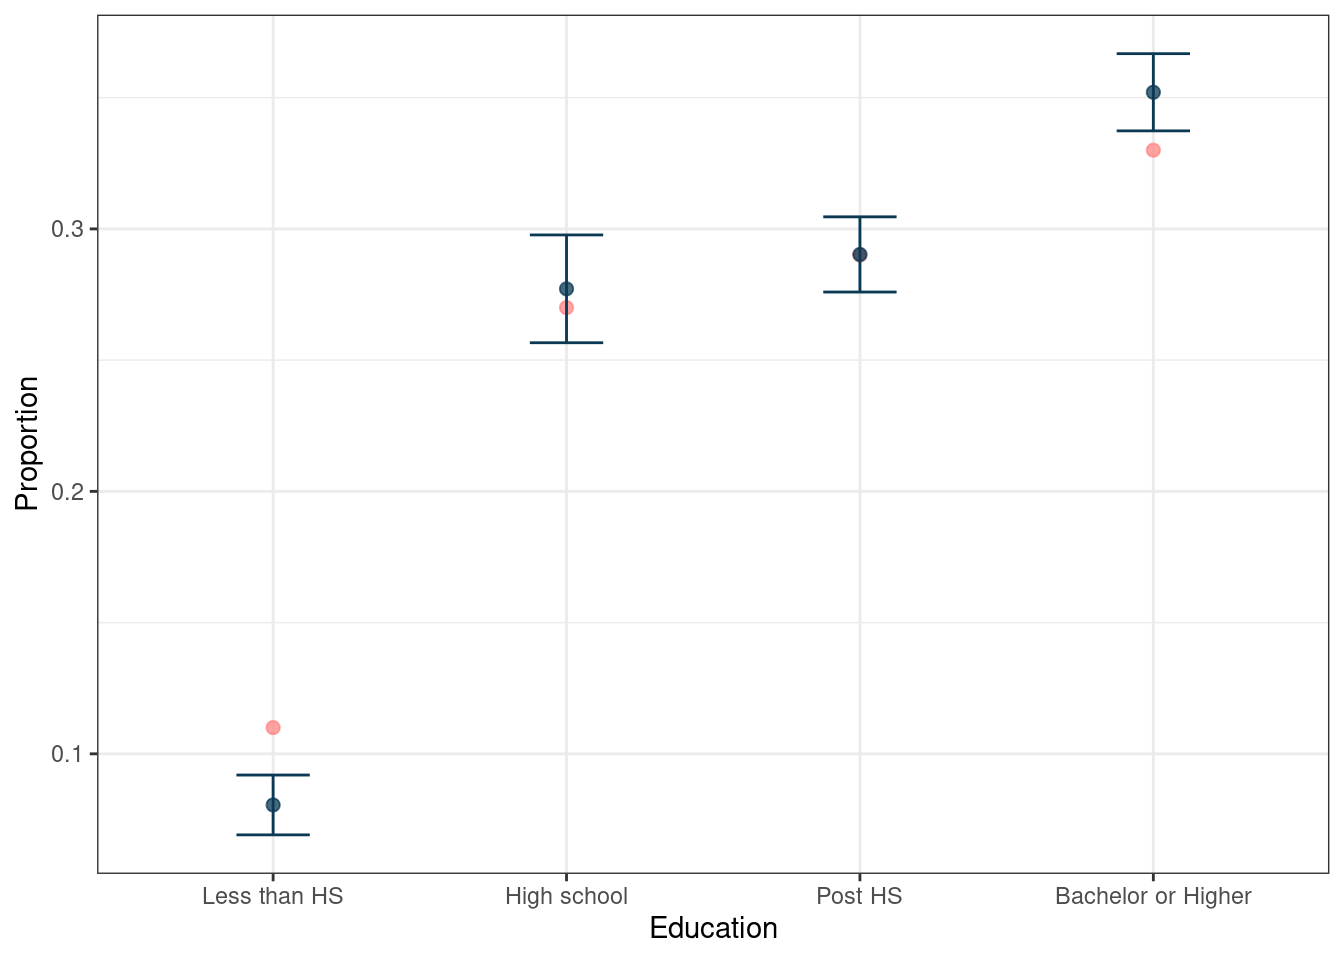
\includegraphics{bookdown_files/figure-latex/stattest-chi-ex1-graph-1} \caption{Expected and observed proportions of education, showing the confidence intervals for the expected proportions and whether the observed proportions lie within them.}\label{fig:stattest-chi-ex1-graph}
\end{figure}

\hypertarget{stattest-chi-ex2}{%
\subsubsection*{Example 2: Test of Independence}\label{stattest-chi-ex2}}


ANES asked respondents two questions about trust:

\begin{itemize}
\tightlist
\item
  How often can you trust the federal government to do what is right?
\item
  How often can you trust other people?
\end{itemize}

If we want to see if the distributions of these two questions are similar or not, we can conduct a test of independence. Here is how the hypothesis could be set up:

\begin{itemize}
\tightlist
\item
  \(H_0:\) People's trust in the federal government and their trust in other people are independent (i.e., \emph{not} related)
\item
  \(H_A:\) People's trust in the federal government and their trust in other people are \emph{not} independent (i.e., they are related)
\end{itemize}

To conduct this in R, we use the \texttt{svychisq()} function to compare the two variables:

\begin{Shaded}
\begin{Highlighting}[]
\NormalTok{chi\_ex2 }\OtherTok{\textless{}{-}}\NormalTok{ anes\_des }\SpecialCharTok{\%\textgreater{}\%}
  \FunctionTok{svychisq}\NormalTok{(}
    \AttributeTok{formula =} \SpecialCharTok{\textasciitilde{}}\NormalTok{ TrustGovernment }\SpecialCharTok{+}\NormalTok{ TrustPeople,}
    \AttributeTok{design =}\NormalTok{ .,}
    \AttributeTok{statistic =} \StringTok{"Wald"}\NormalTok{,}
    \AttributeTok{na.rm =} \ConstantTok{TRUE}
\NormalTok{  )}

\NormalTok{chi\_ex2}
\end{Highlighting}
\end{Shaded}

\begin{verbatim}
## 
##  Design-based Wald test of association
## 
## data:  NextMethod()
## F = 21, ndf = 16, ddf = 51, p-value <2e-16
\end{verbatim}

The output from \texttt{svychisq()} indicates that the distribution of people's trust in the federal government and their trust in other people are \emph{not} independent, meaning that they are related. Let's output the distributions in a table to see the relationship. The \texttt{observed} output from the test provides a cross-tabulation of the counts for each category:

\begin{Shaded}
\begin{Highlighting}[]
\NormalTok{chi\_ex2}\SpecialCharTok{$}\NormalTok{observed}
\end{Highlighting}
\end{Shaded}

\begin{verbatim}
##                      TrustPeople
## TrustGovernment         Always Most of the time About half the time
##   Always                16.470           25.009              31.848
##   Most of the time      11.020          539.377             196.258
##   About half the time   11.772          934.858             861.971
##   Some of the time      17.007         1353.779             839.863
##   Never                  3.174          236.785             174.272
##                      TrustPeople
## TrustGovernment       Some of the time    Never
##   Always                        36.854    5.523
##   Most of the time             206.556   27.184
##   About half the time          428.871   65.024
##   Some of the time             932.628   89.596
##   Never                        217.994  189.307
\end{verbatim}

However, as researchers, we often want to know about the proportions and not just the respondent counts from the survey. There are a couple of different ways that we can do this. The first is using the counts from \texttt{chi\_ex2\$observed} to calculate the proportion. We can then pivot the table to create a cross-tabulation similar to the counts table above. Adding \texttt{group\_by()} to the code means that we are obtaining the proportions within each level of that variable. In this case, we are looking at the distribution of \texttt{TrustGovernment} for each level of \texttt{TrustPeople}. The resulting table is shown in Table \ref{tab:stattest-chi-ex2-prop1-tab} and in Chapter \ref{c08-communicating-results}, we will discuss more on how to make publication-quality tables like this.

\begin{Shaded}
\begin{Highlighting}[]
\NormalTok{chi\_ex2\_table }\OtherTok{\textless{}{-}}\NormalTok{ chi\_ex2}\SpecialCharTok{$}\NormalTok{observed }\SpecialCharTok{\%\textgreater{}\%}
  \FunctionTok{as\_tibble}\NormalTok{() }\SpecialCharTok{\%\textgreater{}\%}
  \FunctionTok{group\_by}\NormalTok{(TrustPeople) }\SpecialCharTok{\%\textgreater{}\%}
  \FunctionTok{mutate}\NormalTok{(}\AttributeTok{prop =} \FunctionTok{round}\NormalTok{(n }\SpecialCharTok{/} \FunctionTok{sum}\NormalTok{(n), }\DecValTok{3}\NormalTok{)) }\SpecialCharTok{\%\textgreater{}\%}
  \FunctionTok{select}\NormalTok{(}\SpecialCharTok{{-}}\NormalTok{n) }\SpecialCharTok{\%\textgreater{}\%}
  \FunctionTok{pivot\_wider}\NormalTok{(}\AttributeTok{names\_from =}\NormalTok{ TrustPeople, }\AttributeTok{values\_from =}\NormalTok{ prop) }\SpecialCharTok{\%\textgreater{}\%}
  \FunctionTok{gt}\NormalTok{(}\AttributeTok{rowname\_col =} \StringTok{"TrustGovernment"}\NormalTok{) }\SpecialCharTok{\%\textgreater{}\%}
  \FunctionTok{tab\_stubhead}\NormalTok{(}\AttributeTok{label =} \StringTok{"Trust in Government"}\NormalTok{) }\SpecialCharTok{\%\textgreater{}\%}
  \FunctionTok{tab\_spanner}\NormalTok{(}
    \AttributeTok{label =} \StringTok{"Trust in People"}\NormalTok{,}
    \AttributeTok{columns =} \FunctionTok{everything}\NormalTok{()}
\NormalTok{  ) }\SpecialCharTok{\%\textgreater{}\%}
  \FunctionTok{cols\_label}\NormalTok{(}
    \StringTok{\textasciigrave{}}\AttributeTok{Most of the time}\StringTok{\textasciigrave{}} \OtherTok{=} \FunctionTok{md}\NormalTok{(}\StringTok{"Most of\textless{}br /\textgreater{}the time"}\NormalTok{),}
    \StringTok{\textasciigrave{}}\AttributeTok{About half the time}\StringTok{\textasciigrave{}} \OtherTok{=} \FunctionTok{md}\NormalTok{(}\StringTok{"About half\textless{}br /\textgreater{}the time"}\NormalTok{),}
    \StringTok{\textasciigrave{}}\AttributeTok{Some of the time}\StringTok{\textasciigrave{}} \OtherTok{=} \FunctionTok{md}\NormalTok{(}\StringTok{"Some of\textless{}br /\textgreater{}the time"}\NormalTok{)}
\NormalTok{  )}
\end{Highlighting}
\end{Shaded}

\begin{Shaded}
\begin{Highlighting}[]
\NormalTok{chi\_ex2\_table}
\end{Highlighting}
\end{Shaded}



\begin{longtable}{l|rrrrr}
\caption{\label{tab:stattest-chi-ex2-prop1-tab}Proportion of adults in the U.S. by levels of trust in people and government, ANES 2020}\\
\toprule
\multicolumn{1}{l}{} & \multicolumn{5}{c}{Trust in People} \\ 
\cmidrule(lr){2-6}
\multicolumn{1}{l}{Trust in Government} & Always & Most ofthe time & About halfthe time & Some ofthe time & Never \\ 
\midrule
Always & 0.277 & 0.008 & 0.015 & 0.020 & 0.015 \\ 
Most of the time & 0.185 & 0.175 & 0.093 & 0.113 & 0.072 \\ 
About half the time & 0.198 & 0.303 & 0.410 & 0.235 & 0.173 \\ 
Some of the time & 0.286 & 0.438 & 0.399 & 0.512 & 0.238 \\ 
Never & 0.053 & 0.077 & 0.083 & 0.120 & 0.503 \\ 
\bottomrule
\end{longtable}

In Table \ref{tab:stattest-chi-ex2-prop1-tab}, each column sums to 1. For example, we can say that it is estimated that of people who always trust in people, 27.7\% also always trust in government based on the top-left cell but 5.3\% never trust in government.

The second option is to use \texttt{group\_by()} and \texttt{survey\_mean()} functions to calculate the proportions from the ANES design object. A reminder that with more than one variable listed in the \texttt{group\_by()} statement, the proportions are within the first variable listed. As mentioned above, we are looking at the distribution of \texttt{TrustGovernment} for each level of \texttt{TrustPeople}.

\begin{Shaded}
\begin{Highlighting}[]
\NormalTok{chi\_ex2\_obs }\OtherTok{\textless{}{-}}\NormalTok{ anes\_des }\SpecialCharTok{\%\textgreater{}\%}
  \FunctionTok{drop\_na}\NormalTok{(TrustPeople, TrustGovernment) }\SpecialCharTok{\%\textgreater{}\%}
  \FunctionTok{group\_by}\NormalTok{(TrustPeople, TrustGovernment) }\SpecialCharTok{\%\textgreater{}\%}
  \FunctionTok{summarize}\NormalTok{(}
    \AttributeTok{Observed =} \FunctionTok{round}\NormalTok{(}\FunctionTok{survey\_mean}\NormalTok{(}\AttributeTok{vartype =} \StringTok{"ci"}\NormalTok{), }\DecValTok{3}\NormalTok{),}
    \AttributeTok{.groups =} \StringTok{"drop"}
\NormalTok{  )}

\NormalTok{chi\_ex2\_obs\_table }\OtherTok{\textless{}{-}}\NormalTok{ chi\_ex2\_obs }\SpecialCharTok{\%\textgreater{}\%}
  \FunctionTok{mutate}\NormalTok{(}\AttributeTok{prop =} \FunctionTok{paste0}\NormalTok{(}
\NormalTok{    Observed, }\StringTok{" ("}\NormalTok{, Observed\_low, }\StringTok{", "}\NormalTok{,}
\NormalTok{    Observed\_upp, }\StringTok{")"}
\NormalTok{  )) }\SpecialCharTok{\%\textgreater{}\%}
  \FunctionTok{select}\NormalTok{(TrustGovernment, TrustPeople, prop) }\SpecialCharTok{\%\textgreater{}\%}
  \FunctionTok{pivot\_wider}\NormalTok{(}\AttributeTok{names\_from =}\NormalTok{ TrustPeople, }\AttributeTok{values\_from =}\NormalTok{ prop) }\SpecialCharTok{\%\textgreater{}\%}
  \FunctionTok{gt}\NormalTok{(}\AttributeTok{rowname\_col =} \StringTok{"TrustGovernment"}\NormalTok{) }\SpecialCharTok{\%\textgreater{}\%}
  \FunctionTok{tab\_stubhead}\NormalTok{(}\AttributeTok{label =} \StringTok{"Trust in Government"}\NormalTok{) }\SpecialCharTok{\%\textgreater{}\%}
  \FunctionTok{tab\_spanner}\NormalTok{(}
    \AttributeTok{label =} \StringTok{"Trust in People"}\NormalTok{,}
    \AttributeTok{columns =} \FunctionTok{everything}\NormalTok{()}
\NormalTok{  ) }\SpecialCharTok{\%\textgreater{}\%}
  \FunctionTok{tab\_options}\NormalTok{(}\AttributeTok{page.orientation =} \StringTok{"landscape"}\NormalTok{)}
\end{Highlighting}
\end{Shaded}

\begin{Shaded}
\begin{Highlighting}[]
\NormalTok{chi\_ex2\_obs\_table}
\end{Highlighting}
\end{Shaded}



\begin{longtable}{l|rrrrr}
\caption{\label{tab:stattest-chi-ex2-prop2-tab}Proportion of adults in the U.S. by levels of trust in people and government with confidence intervals, ANES 2020}\\
\toprule
\multicolumn{1}{l}{} & \multicolumn{5}{c}{Trust in People} \\ 
\cmidrule(lr){2-6}
\multicolumn{1}{l}{Trust in Government} & Always & Most of the time & About half the time & Some of the time & Never \\ 
\midrule
Always & 0.277 (0.11, 0.444) & 0.008 (0.004, 0.012) & 0.015 (0.006, 0.024) & 0.02 (0.008, 0.033) & 0.015 (0, 0.029) \\ 
Most of the time & 0.185 (-0.009, 0.38) & 0.175 (0.157, 0.192) & 0.093 (0.078, 0.109) & 0.113 (0.085, 0.141) & 0.072 (0.021, 0.123) \\ 
About half the time & 0.198 (0.046, 0.35) & 0.303 (0.281, 0.324) & 0.41 (0.378, 0.441) & 0.235 (0.2, 0.271) & 0.173 (0.099, 0.246) \\ 
Some of the time & 0.286 (0.069, 0.503) & 0.438 (0.415, 0.462) & 0.399 (0.365, 0.433) & 0.512 (0.481, 0.543) & 0.238 (0.178, 0.298) \\ 
Never & 0.053 (-0.01, 0.117) & 0.077 (0.064, 0.089) & 0.083 (0.063, 0.103) & 0.12 (0.097, 0.142) & 0.503 (0.422, 0.583) \\ 
\bottomrule
\end{longtable}

Both methods produce the same output as the \texttt{svychisq()} function does account for the survey design. However, calculating the proportions directly from the design object means we can also obtain the variance information. In this case, the table output displays the survey estimate followed by the confidence intervals. Based on the output, we can see that of those who never trust people, 50.3\% also never trust the government, while the proportions of never trusting the government are much lower for each of the other levels of trusting people.

We may find it easier to look at these proportions graphically. We can use \texttt{ggplot()} and facets to provide an overview as shown below to create Figure \ref{fig:stattest-chi-ex2-graph}:

\begin{Shaded}
\begin{Highlighting}[]
\NormalTok{chi\_ex2\_obs }\SpecialCharTok{\%\textgreater{}\%}
  \FunctionTok{mutate}\NormalTok{(}
    \AttributeTok{TrustPeople =}
      \FunctionTok{fct\_reorder}\NormalTok{(}
        \FunctionTok{str\_c}\NormalTok{(}\StringTok{"Trust in People:}\SpecialCharTok{\textbackslash{}n}\StringTok{"}\NormalTok{, TrustPeople),}
        \FunctionTok{order}\NormalTok{(TrustPeople)}
\NormalTok{      )}
\NormalTok{  ) }\SpecialCharTok{\%\textgreater{}\%}
  \FunctionTok{ggplot}\NormalTok{(}\FunctionTok{aes}\NormalTok{(}\AttributeTok{x =}\NormalTok{ TrustGovernment, }\AttributeTok{y =}\NormalTok{ Observed, }\AttributeTok{color =}\NormalTok{ TrustGovernment)) }\SpecialCharTok{+}
  \FunctionTok{facet\_wrap}\NormalTok{(}\SpecialCharTok{\textasciitilde{}}\NormalTok{TrustPeople, }\AttributeTok{ncol =} \DecValTok{5}\NormalTok{) }\SpecialCharTok{+}
  \FunctionTok{geom\_point}\NormalTok{() }\SpecialCharTok{+}
  \FunctionTok{geom\_errorbar}\NormalTok{(}\FunctionTok{aes}\NormalTok{(}\AttributeTok{ymin =}\NormalTok{ Observed\_low, }\AttributeTok{ymax =}\NormalTok{ Observed\_upp)) }\SpecialCharTok{+}
  \FunctionTok{ylab}\NormalTok{(}\StringTok{"Proportion"}\NormalTok{) }\SpecialCharTok{+}
  \FunctionTok{xlab}\NormalTok{(}\StringTok{""}\NormalTok{) }\SpecialCharTok{+}
  \FunctionTok{theme\_bw}\NormalTok{() }\SpecialCharTok{+}
  \FunctionTok{scale\_color\_manual}\NormalTok{(}\AttributeTok{name =} \StringTok{"Trust in Government"}\NormalTok{, }\AttributeTok{values =}\NormalTok{ book\_colors) }\SpecialCharTok{+}
  \FunctionTok{theme}\NormalTok{(}
    \AttributeTok{axis.text.x =} \FunctionTok{element\_blank}\NormalTok{(),}
    \AttributeTok{axis.ticks.x =} \FunctionTok{element\_blank}\NormalTok{(),}
    \AttributeTok{legend.position =} \StringTok{"bottom"}
\NormalTok{  ) }\SpecialCharTok{+}
  \FunctionTok{guides}\NormalTok{(}\AttributeTok{col =} \FunctionTok{guide\_legend}\NormalTok{(}\AttributeTok{nrow =} \DecValTok{2}\NormalTok{))}
\end{Highlighting}
\end{Shaded}

\begin{figure}
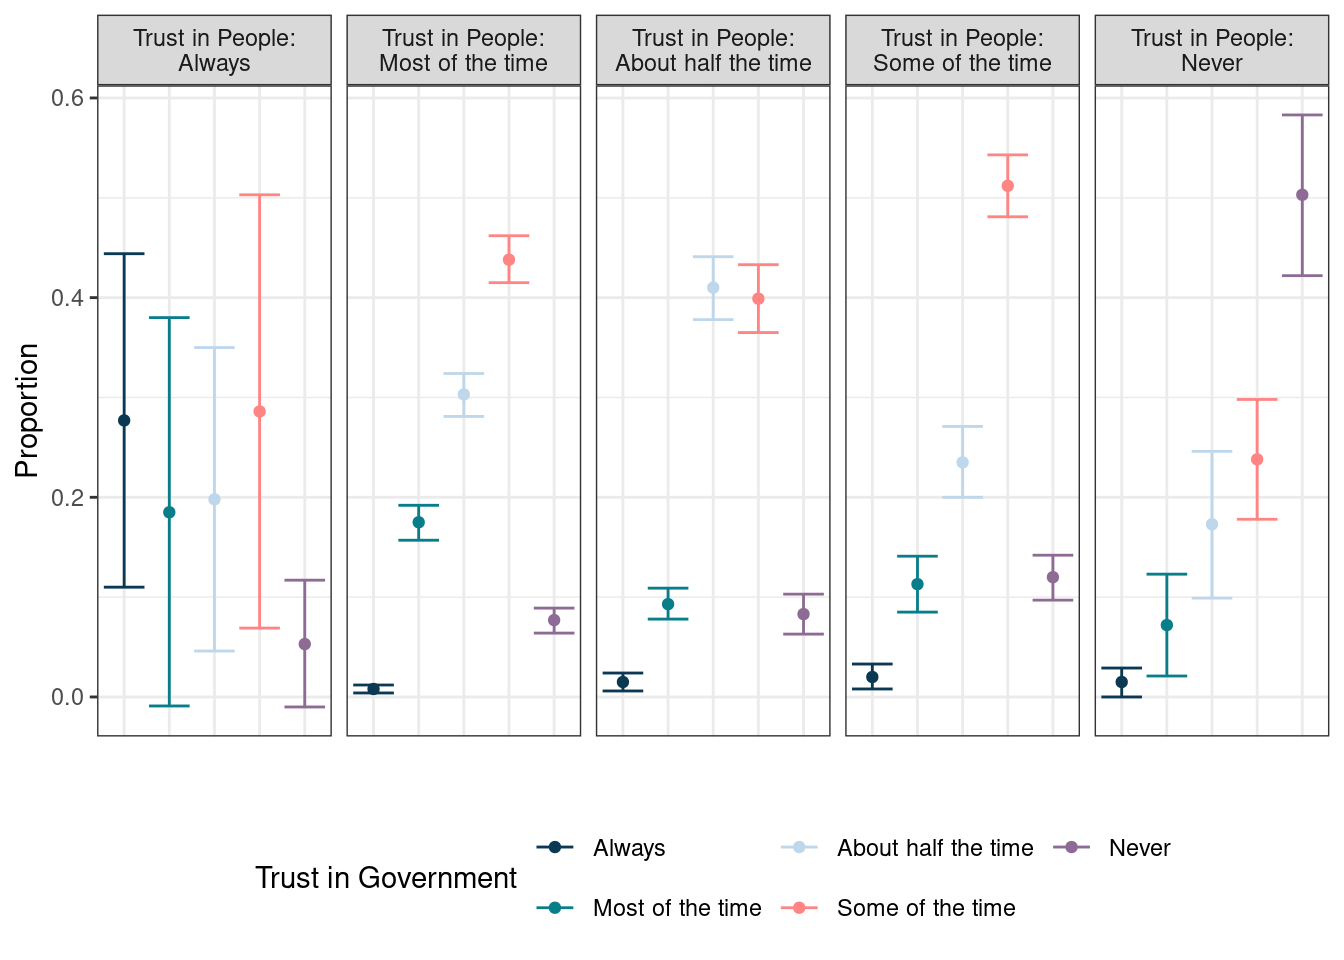
\includegraphics{bookdown_files/figure-latex/stattest-chi-ex2-graph-1} \caption{Proportion of adults in the U.S. by levels of trust in people and government with confidence intervals, ANES 2020}\label{fig:stattest-chi-ex2-graph}
\end{figure}

\hypertarget{stattest-chi-ex3}{%
\subsubsection*{Example 3: Test of Homogeneity}\label{stattest-chi-ex3}}


Researchers and politicians often look at specific demographics each election cycle to understand how each group is leaning or voting toward candidates. The ANES data are collected post-election, but we can still see if there are differences in how specific demographic groups voted.

If we want to see if there is a difference in how each age group voted for the 2020 candidates, this would be a test of homogeneity, and we can set up the hypothesis as follows:

\begin{align*}
H_0: p_{1_{Biden}} &= p_{1_{Trump}} = p_{1_{Other}},\\
    p_{2_{Biden}} &= p_{2_{Trump}} = p_{2_{Other}},\\
    p_{3_{Biden}} &= p_{3_{Trump}} = p_{3_{Other}},\\
    p_{4_{Biden}} &= p_{4_{Trump}} = p_{4_{Other}},\\
    p_{5_{Biden}} &= p_{5_{Trump}} = p_{5_{Other}},\\
    p_{6_{Biden}} &= p_{6_{Trump}} = p_{6_{Other}}
  \end{align*}
where \(p_{i_{Biden}}\) is the observed proportion of each age group (\(i\)) that voted for Joseph Biden, \(p_{i_{Trump}}\) is the observed proportion of each age group (\(i\)) that voted for Donald Trump, and \(p_{i_{Other}}\) is the observed proportion of each age group (\(i\)) that voted for another candidate

\begin{itemize}
\tightlist
\item
  \(H_A:\) at least one category of \(p_{i_{Biden}}\) does not match \(p_{i_{Trump}}\) or \(p_{i_{Other}}\)
\end{itemize}

To conduct this in R, we use the \texttt{svychisq()} function to compare the two variables:

\begin{Shaded}
\begin{Highlighting}[]
\NormalTok{chi\_ex3 }\OtherTok{\textless{}{-}}\NormalTok{ anes\_des }\SpecialCharTok{\%\textgreater{}\%}
  \FunctionTok{drop\_na}\NormalTok{(VotedPres2020\_selection, AgeGroup) }\SpecialCharTok{\%\textgreater{}\%}
  \FunctionTok{svychisq}\NormalTok{(}
    \AttributeTok{formula =} \SpecialCharTok{\textasciitilde{}}\NormalTok{ AgeGroup }\SpecialCharTok{+}\NormalTok{ VotedPres2020\_selection,}
    \AttributeTok{design =}\NormalTok{ .,}
    \AttributeTok{statistic =} \StringTok{"Chisq"}\NormalTok{,}
    \AttributeTok{na.rm =} \ConstantTok{TRUE}
\NormalTok{  )}

\NormalTok{chi\_ex3}
\end{Highlighting}
\end{Shaded}

\begin{verbatim}
## 
##  Pearson's X^2: Rao & Scott adjustment
## 
## data:  NextMethod()
## X-squared = 171, df = 10, p-value <2e-16
\end{verbatim}

The output from \texttt{svychisq()} indicates a difference in how each age group voted in the 2020 election. To get a better idea of the different distributions, let's output proportions to see the relationship. As we learned in Example 2 above, we can use \texttt{chi\_ex3\$observed}, or if we want to get the variance information (which is crucial with survey data), we can use \texttt{survey\_mean()}. Remember, when we have two variables in \texttt{group\_by()}, we obtain the proportions within each level of the variable listed. In this case, we are looking at the distribution of \texttt{AgeGroup} for each level of \texttt{VotedPres2020\_selection}.

\begin{Shaded}
\begin{Highlighting}[]
\NormalTok{chi\_ex3\_obs }\OtherTok{\textless{}{-}}\NormalTok{ anes\_des }\SpecialCharTok{\%\textgreater{}\%}
  \FunctionTok{filter}\NormalTok{(VotedPres2020 }\SpecialCharTok{==} \StringTok{"Yes"}\NormalTok{) }\SpecialCharTok{\%\textgreater{}\%}
  \FunctionTok{drop\_na}\NormalTok{(VotedPres2020\_selection, AgeGroup) }\SpecialCharTok{\%\textgreater{}\%}
  \FunctionTok{group\_by}\NormalTok{(VotedPres2020\_selection, AgeGroup) }\SpecialCharTok{\%\textgreater{}\%}
  \FunctionTok{summarize}\NormalTok{(}\AttributeTok{Observed =} \FunctionTok{round}\NormalTok{(}\FunctionTok{survey\_mean}\NormalTok{(}\AttributeTok{vartype =} \StringTok{"ci"}\NormalTok{), }\DecValTok{3}\NormalTok{))}

\NormalTok{chi\_ex3\_obs\_table }\OtherTok{\textless{}{-}}\NormalTok{ chi\_ex3\_obs }\SpecialCharTok{\%\textgreater{}\%}
  \FunctionTok{mutate}\NormalTok{(}\AttributeTok{prop =} \FunctionTok{paste0}\NormalTok{(}
\NormalTok{    Observed, }\StringTok{" ("}\NormalTok{, Observed\_low, }\StringTok{", "}\NormalTok{,}
\NormalTok{    Observed\_upp, }\StringTok{")"}
\NormalTok{  )) }\SpecialCharTok{\%\textgreater{}\%}
  \FunctionTok{select}\NormalTok{(AgeGroup, VotedPres2020\_selection, prop) }\SpecialCharTok{\%\textgreater{}\%}
  \FunctionTok{pivot\_wider}\NormalTok{(}
    \AttributeTok{names\_from =}\NormalTok{ VotedPres2020\_selection,}
    \AttributeTok{values\_from =}\NormalTok{ prop}
\NormalTok{  ) }\SpecialCharTok{\%\textgreater{}\%}
  \FunctionTok{gt}\NormalTok{(}\AttributeTok{rowname\_col =} \StringTok{"AgeGroup"}\NormalTok{) }\SpecialCharTok{\%\textgreater{}\%}
  \FunctionTok{tab\_stubhead}\NormalTok{(}\AttributeTok{label =} \StringTok{"Age Group"}\NormalTok{)}
\end{Highlighting}
\end{Shaded}

\begin{Shaded}
\begin{Highlighting}[]
\NormalTok{chi\_ex3\_obs\_table}
\end{Highlighting}
\end{Shaded}



\begin{longtable}{l|rrr}
\caption{\label{tab:stattest-chi-ex3-tab}Distribution of age group by presidential candidate selection with confidence intervals}\\
\toprule
\multicolumn{1}{l}{Age Group} & Biden & Trump & Other \\ 
\midrule
18-29 & 0.203 (0.177, 0.229) & 0.113 (0.095, 0.132) & 0.221 (0.144, 0.298) \\ 
30-39 & 0.168 (0.152, 0.184) & 0.146 (0.125, 0.168) & 0.302 (0.21, 0.394) \\ 
40-49 & 0.163 (0.146, 0.18) & 0.157 (0.137, 0.177) & 0.21 (0.13, 0.29) \\ 
50-59 & 0.152 (0.135, 0.17) & 0.229 (0.202, 0.256) & 0.104 (0.04, 0.168) \\ 
60-69 & 0.177 (0.159, 0.196) & 0.193 (0.173, 0.213) & 0.103 (0.025, 0.182) \\ 
70 or older & 0.136 (0.123, 0.149) & 0.161 (0.143, 0.179) & 0.06 (0.01, 0.109) \\ 
\bottomrule
\end{longtable}

We can see that the age group distribution that voted for Biden and other candidates was younger than those that voted for Trump. For example, of those who voted for Biden, 20.4\% were in the 18-29 age group, compared to only 11.4\% of those who voted for Trump were in that age group. On the other side, 23.4\% of those who voted for Trump were in the 50-59 age group compared to only 15.4\% of those who voted for Biden.

\hypertarget{stattest-exercises}{%
\section{Exercises}\label{stattest-exercises}}

The exercises use the design objects \texttt{anes\_des} and \texttt{recs\_des} as provided in the Prerequisites box in the \protect\hyperlink{c06-statistical-testing}{beginning of the chapter}. Here are some exercises for practicing conducting t-tests using \texttt{svyttest()}:

\begin{enumerate}
\def\labelenumi{\arabic{enumi}.}
\tightlist
\item
  Using the RECS data, do more than 50\% of U.S. households use AC (\texttt{ACUsed})?
\end{enumerate}

\begin{Shaded}
\begin{Highlighting}[]
\NormalTok{ttest\_solution1 }\OtherTok{\textless{}{-}}\NormalTok{ recs\_des }\SpecialCharTok{\%\textgreater{}\%}
  \FunctionTok{svyttest}\NormalTok{(}
    \AttributeTok{design =}\NormalTok{ .,}
    \AttributeTok{formula =}\NormalTok{ ((ACUsed }\SpecialCharTok{==} \ConstantTok{TRUE}\NormalTok{) }\SpecialCharTok{{-}} \FloatTok{0.5}\NormalTok{) }\SpecialCharTok{\textasciitilde{}} \DecValTok{0}\NormalTok{,}
    \AttributeTok{na.rm =} \ConstantTok{TRUE}
\NormalTok{  )}

\NormalTok{ttest\_solution1}
\end{Highlighting}
\end{Shaded}

\begin{verbatim}
## 
##  Design-based one-sample t-test
## 
## data:  ((ACUsed == TRUE) - 0.5) ~ 0
## t = 126, df = 58, p-value <2e-16
## alternative hypothesis: true mean is not equal to 0
## 95 percent confidence interval:
##  0.3804 0.3927
## sample estimates:
##   mean 
## 0.3865
\end{verbatim}

\begin{enumerate}
\def\labelenumi{\arabic{enumi}.}
\setcounter{enumi}{1}
\tightlist
\item
  Using the RECS data, does the average temperature that U.S. households set their thermostats to differ between the day and night in the winter (\texttt{WinterTempDay} and \texttt{WinterTempNight})?
\end{enumerate}

\begin{Shaded}
\begin{Highlighting}[]
\NormalTok{ttest\_solution2 }\OtherTok{\textless{}{-}}\NormalTok{ recs\_des }\SpecialCharTok{\%\textgreater{}\%}
  \FunctionTok{svyttest}\NormalTok{(}
    \AttributeTok{design =}\NormalTok{ .,}
    \AttributeTok{formula =}\NormalTok{ WinterTempDay }\SpecialCharTok{{-}}\NormalTok{ WinterTempNight }\SpecialCharTok{\textasciitilde{}} \DecValTok{0}\NormalTok{,}
    \AttributeTok{na.rm =} \ConstantTok{TRUE}
\NormalTok{  )}

\NormalTok{ttest\_solution2}
\end{Highlighting}
\end{Shaded}

\begin{verbatim}
## 
##  Design-based one-sample t-test
## 
## data:  WinterTempDay - WinterTempNight ~ 0
## t = 46, df = 58, p-value <2e-16
## alternative hypothesis: true mean is not equal to 0
## 95 percent confidence interval:
##  1.594 1.740
## sample estimates:
##  mean 
## 1.667
\end{verbatim}

\begin{enumerate}
\def\labelenumi{\arabic{enumi}.}
\setcounter{enumi}{2}
\tightlist
\item
  Using the ANES data, does the average age (\texttt{Age}) of those who voted for Joseph Biden in 2020 (\texttt{VotedPres2020\_selection}) differ from those who voted for another candidate?
\end{enumerate}

\begin{Shaded}
\begin{Highlighting}[]
\NormalTok{ttest\_solution3 }\OtherTok{\textless{}{-}}\NormalTok{ anes\_des }\SpecialCharTok{\%\textgreater{}\%}
  \FunctionTok{svyttest}\NormalTok{(}
    \AttributeTok{design =}\NormalTok{ .,}
    \AttributeTok{formula =}\NormalTok{ Age }\SpecialCharTok{\textasciitilde{}}\NormalTok{ VotedPres2020\_selection }\SpecialCharTok{==} \StringTok{"Biden"}\NormalTok{,}
    \AttributeTok{na.rm =} \ConstantTok{TRUE}
\NormalTok{  )}

\NormalTok{ttest\_solution3}
\end{Highlighting}
\end{Shaded}

\begin{verbatim}
## 
##  Design-based t-test
## 
## data:  Age ~ VotedPres2020_selection == "Biden"
## t = -6, df = 50, p-value = 2e-07
## alternative hypothesis: true difference in mean is not equal to 0
## 95 percent confidence interval:
##  -4.809 -2.388
## sample estimates:
## difference in mean 
##             -3.598
\end{verbatim}

\begin{enumerate}
\def\labelenumi{\arabic{enumi}.}
\setcounter{enumi}{3}
\tightlist
\item
  If you wanted to determine if the political party affiliation differed for males and females, what test would you use?
\end{enumerate}

\begin{enumerate}
\def\labelenumi{\alph{enumi}.}
\tightlist
\item
  Goodness of fit test (\texttt{svygofchisq()})
\item
  Test of independence (\texttt{svychisq()})
\item
  Test of homogeneity (\texttt{svychisq()})
\end{enumerate}

\begin{Shaded}
\begin{Highlighting}[]
\NormalTok{chisq\_solution1 }\OtherTok{\textless{}{-}} \StringTok{"c. Test of homogeneity (\textasciigrave{}svychisq()\textasciigrave{})"}
\NormalTok{chisq\_solution1}
\end{Highlighting}
\end{Shaded}

\begin{verbatim}
## [1] "c. Test of homogeneity (`svychisq()`)"
\end{verbatim}

\begin{enumerate}
\def\labelenumi{\arabic{enumi}.}
\setcounter{enumi}{4}
\tightlist
\item
  In the RECS data, is there a relationship between the type of housing unit (\texttt{HousingUnitType}) and the year the house was built (\texttt{YearMade})?
\end{enumerate}

\begin{Shaded}
\begin{Highlighting}[]
\NormalTok{chisq\_solution2 }\OtherTok{\textless{}{-}}\NormalTok{ recs\_des }\SpecialCharTok{\%\textgreater{}\%}
  \FunctionTok{svychisq}\NormalTok{(}
    \AttributeTok{formula =} \SpecialCharTok{\textasciitilde{}}\NormalTok{ HousingUnitType }\SpecialCharTok{+}\NormalTok{ YearMade,}
    \AttributeTok{design =}\NormalTok{ .,}
    \AttributeTok{statistic =} \StringTok{"Wald"}\NormalTok{,}
    \AttributeTok{na.rm =} \ConstantTok{TRUE}
\NormalTok{  )}

\NormalTok{chisq\_solution2}
\end{Highlighting}
\end{Shaded}

\begin{verbatim}
## 
##  Design-based Wald test of association
## 
## data:  NextMethod()
## F = 68, ndf = 32, ddf = 59, p-value <2e-16
\end{verbatim}

\begin{enumerate}
\def\labelenumi{\arabic{enumi}.}
\setcounter{enumi}{5}
\tightlist
\item
  In the ANES data, is there a difference in the distribution of gender (\texttt{Gender}) across early voting status in 2020 (\texttt{EarlyVote2020})?
\end{enumerate}

\begin{Shaded}
\begin{Highlighting}[]
\NormalTok{chisq\_solution3 }\OtherTok{\textless{}{-}}\NormalTok{ anes\_des }\SpecialCharTok{\%\textgreater{}\%}
  \FunctionTok{svychisq}\NormalTok{(}
    \AttributeTok{formula =} \SpecialCharTok{\textasciitilde{}}\NormalTok{ Gender }\SpecialCharTok{+}\NormalTok{ EarlyVote2020,}
    \AttributeTok{design =}\NormalTok{ .,}
    \AttributeTok{statistic =} \StringTok{"F"}\NormalTok{,}
    \AttributeTok{na.rm =} \ConstantTok{TRUE}
\NormalTok{  )}

\NormalTok{chisq\_solution3}
\end{Highlighting}
\end{Shaded}

\begin{verbatim}
## 
##  Pearson's X^2: Rao & Scott adjustment
## 
## data:  NextMethod()
## F = 4.5, ndf = 1, ddf = 51, p-value = 0.04
\end{verbatim}

\hypertarget{c07-modeling}{%
\chapter{Modeling}\label{c07-modeling}}

\begin{prereqbox}{Prerequisites}

For this chapter, load the following packages:

\begin{Shaded}
\begin{Highlighting}[]
\FunctionTok{library}\NormalTok{(tidyverse)}
\FunctionTok{library}\NormalTok{(survey)}
\FunctionTok{library}\NormalTok{(srvyr)}
\FunctionTok{library}\NormalTok{(srvyrexploR)}
\FunctionTok{library}\NormalTok{(broom)}
\FunctionTok{library}\NormalTok{(gt)}
\FunctionTok{library}\NormalTok{(prettyunits)}
\end{Highlighting}
\end{Shaded}

We will be using data from ANES and RECS described in Chapter \ref{c04-getting-started}. As a reminder, here is the code to create the design objects for each to use throughout this chapter. For ANES, we need to adjust the weight so it sums to the population instead of the sample (see the ANES documentation and Chapter \ref{c04-getting-started} for more information).

\begin{Shaded}
\begin{Highlighting}[]
\NormalTok{targetpop }\OtherTok{\textless{}{-}} \DecValTok{231592693}
\FunctionTok{data}\NormalTok{(anes\_2020)}

\NormalTok{anes\_adjwgt }\OtherTok{\textless{}{-}}\NormalTok{ anes\_2020 }\SpecialCharTok{\%\textgreater{}\%}
  \FunctionTok{mutate}\NormalTok{(}\AttributeTok{Weight =}\NormalTok{ Weight }\SpecialCharTok{/} \FunctionTok{sum}\NormalTok{(Weight) }\SpecialCharTok{*}\NormalTok{ targetpop)}

\NormalTok{anes\_des }\OtherTok{\textless{}{-}}\NormalTok{ anes\_adjwgt }\SpecialCharTok{\%\textgreater{}\%}
  \FunctionTok{as\_survey\_design}\NormalTok{(}
    \AttributeTok{weights =}\NormalTok{ Weight,}
    \AttributeTok{strata =}\NormalTok{ Stratum,}
    \AttributeTok{ids =}\NormalTok{ VarUnit,}
    \AttributeTok{nest =} \ConstantTok{TRUE}
\NormalTok{  )}
\end{Highlighting}
\end{Shaded}

For RECS, details are included in the RECS documentation and Chapters \ref{c04-getting-started} and \ref{c10-specifying-sample-designs}.

\begin{Shaded}
\begin{Highlighting}[]
\FunctionTok{data}\NormalTok{(recs\_2020)}

\NormalTok{recs\_des }\OtherTok{\textless{}{-}}\NormalTok{ recs\_2020 }\SpecialCharTok{\%\textgreater{}\%}
  \FunctionTok{as\_survey\_rep}\NormalTok{(}
    \AttributeTok{weights =}\NormalTok{ NWEIGHT,}
    \AttributeTok{repweights =}\NormalTok{ NWEIGHT1}\SpecialCharTok{:}\NormalTok{NWEIGHT60,}
    \AttributeTok{type =} \StringTok{"JK1"}\NormalTok{,}
    \AttributeTok{scale =} \DecValTok{59} \SpecialCharTok{/} \DecValTok{60}\NormalTok{,}
    \AttributeTok{mse =} \ConstantTok{TRUE}
\NormalTok{  )}
\end{Highlighting}
\end{Shaded}

\end{prereqbox}

\hypertarget{model-intro}{%
\section{Introduction}\label{model-intro}}

Modeling data is a way for researchers to investigate the relationship between a single dependent variable and one or more independent variables. This builds upon the analyses conducted in Chapter \ref{c06-statistical-testing}, which looked at the relationships between just two variables. For example, in Example 3 in Section \ref{stattest-ttest-examples}, we investigated if there is a relationship between the electrical bill cost and whether or not the household used air-conditioning. However, there are potentially other elements that could go into what the cost of electrical bills are in a household (e.g., outside temperature, desired internal temperature, types and number of appliances, etc.).

T-tests only allow us to investigate the relationship of one independent variable at a time, but using models we can look into multiple variables and even explore interactions between these variables. There are several types of models, but in this chapter we will cover Analysis of Variance (ANOVA) and linear regression models following common normal (Gaussian) and logit models. Jonas Kristoffer Lindeløv has an interesting \href{https://lindeloev.github.io/tests-as-linear/}{discussion} of many statistical tests and models being equivalent to a linear model. For example, a one-way ANOVA is a linear model with one categorical independent variable, and a two-sample t-test is an ANOVA where the independent variable has exactly two levels.

When modeling data, it is helpful to first create an equation that provides an overview as to what it is that we are modeling. The main structure of these models is as follows:

\[y_i=\beta_0 +\sum_{i=1}^p \beta_i x_i + \epsilon_i\]

where \(y_i\) is the outcome, \(\beta_0\) is an intercept, \(x_1, \cdots, x_p\) are the predictors with \(\beta_1, \cdots, \beta_p\) as the associated coefficients, and \(\epsilon_i\) is the error. Not all models will have all components. For example, some models may not include an intercept (\(\beta_0\)), may have interactions between different independent variables (\(x_i\)), or may have different underlying structures for the dependent variable (\(y_i\)). However, all linear models have the independent variables related to the dependent variable in a linear form.

To specify these models in R, the formulas are the same with both survey data and other data. The left side of the formula is the response/dependent variable, and the right side of the formula has the predictor/independent variable(s). There are many symbols used in R to specify the formula.

For example, a linear formula mathematically notated as

\[y_i=\beta_0+\beta_1 x_i+\epsilon_i\] would be specified in R as \texttt{y\textasciitilde{}x} where the intercept is not explicitly included. To fit a model with no intercept, that is,

\[y_i=\beta_1 x_i+\epsilon_i\]
it can be specified in R as \texttt{y\textasciitilde{}x-1}. Formula notation details in R can be found in the help file for formula\footnote{Use \texttt{help(formula)} or \texttt{?formula} in R or find the documentation online at \url{https://stat.ethz.ch/R-manual/R-devel/library/stats/html/formula.html}}. A quick overview of the common formula notation is in Table \ref{tab:notation-common}:

\begin{longtable}[]{@{}
  >{\centering\arraybackslash}p{(\columnwidth - 4\tabcolsep) * \real{0.1238}}
  >{\centering\arraybackslash}p{(\columnwidth - 4\tabcolsep) * \real{0.1619}}
  >{\raggedright\arraybackslash}p{(\columnwidth - 4\tabcolsep) * \real{0.7143}}@{}}
\caption{\label{tab:notation-common} Common symbols in formula notation}\tabularnewline
\toprule\noalign{}
\begin{minipage}[b]{\linewidth}\centering
Symbol
\end{minipage} & \begin{minipage}[b]{\linewidth}\centering
Example
\end{minipage} & \begin{minipage}[b]{\linewidth}\raggedright
Meaning
\end{minipage} \\
\midrule\noalign{}
\endfirsthead
\toprule\noalign{}
\begin{minipage}[b]{\linewidth}\centering
Symbol
\end{minipage} & \begin{minipage}[b]{\linewidth}\centering
Example
\end{minipage} & \begin{minipage}[b]{\linewidth}\raggedright
Meaning
\end{minipage} \\
\midrule\noalign{}
\endhead
\bottomrule\noalign{}
\endlastfoot
+ & \texttt{+x} & include this variable \\
- & \texttt{-x} & delete this variable \\
: & \texttt{x:z} & include the interaction between these variables \\
* & \texttt{x*z} & include these variables and the interactions between them \\
\texttt{\^{}n} & \texttt{(x+y+z)\^{}3} & include these variables and all interactions up to n-way \\
I & \texttt{I(x-z)} & as-is: include a new variable which is calculated inside the parentheses (e.g., x-z, x*z, x/z are possible claculations that could be done) \\
\end{longtable}

There are often multiple ways to specify the same formula. For example, consider the following equation using the \texttt{mtcars} dataset that is built into R:

\[mpg_i=\beta_0+\beta_1cyl_{i}+\beta_2disp_{i}+\beta_3hp_{i}+\beta_4cyl_{i}disp_{i}+\beta_5cyl_{i}hp_{i}+\beta_6disp_{i}hp_{i}+\epsilon_i\]

This could be specified in R code as any of the following:

\begin{itemize}
\tightlist
\item
  \texttt{mpg\ \textasciitilde{}\ (cyl\ +\ disp\ +\ hp)\^{}2}
\item
  \texttt{mpg\ \textasciitilde{}\ cyl\ +\ disp\ +\ hp\ +\ cyl:disp\ +\ cyl:hp\ +\ disp:hp}
\item
  \texttt{mpg\ \textasciitilde{}\ cyl*disp\ +\ cyl*hp\ +\ disp*hp}
\end{itemize}

In the above options, the way the \texttt{:} and \texttt{*} notation are implemented are different. Using \texttt{:} only includes the interactions and not the main effects, while using \texttt{*} includes the main effects and all possible interactions. Table \ref{tab:notation-diffs} provides an overview of the syntax and differences between the two notations.

\begin{longtable}[]{@{}
  >{\centering\arraybackslash}p{(\columnwidth - 4\tabcolsep) * \real{0.1238}}
  >{\centering\arraybackslash}p{(\columnwidth - 4\tabcolsep) * \real{0.1619}}
  >{\raggedright\arraybackslash}p{(\columnwidth - 4\tabcolsep) * \real{0.7143}}@{}}
\caption{\label{tab:notation-diffs} Differences in formulas for \texttt{:} and \texttt{*} code syntax}\tabularnewline
\toprule\noalign{}
\begin{minipage}[b]{\linewidth}\centering
Symbol
\end{minipage} & \begin{minipage}[b]{\linewidth}\centering
Syntax
\end{minipage} & \begin{minipage}[b]{\linewidth}\raggedright
Formula
\end{minipage} \\
\midrule\noalign{}
\endfirsthead
\toprule\noalign{}
\begin{minipage}[b]{\linewidth}\centering
Symbol
\end{minipage} & \begin{minipage}[b]{\linewidth}\centering
Syntax
\end{minipage} & \begin{minipage}[b]{\linewidth}\raggedright
Formula
\end{minipage} \\
\midrule\noalign{}
\endhead
\bottomrule\noalign{}
\endlastfoot
: & \texttt{mpg\ \textasciitilde{}\ cyl:disp:hp} & \( \begin{aligned} mpg_i = &\beta_0+\beta_4cyl_{i}disp_{i}+\beta_5cyl_{i}hp_{i}+ \\& \beta_6disp_{i}hp_{i}+\epsilon_i\end{aligned}\) \\
* & \texttt{mpg\ \textasciitilde{}\ cyl*disp*hp} & \( \begin{aligned} mpg_i= &\beta_0+\beta_1cyl_{i}+\beta_2disp_{i}+\beta_3hp_{i}+\\&        \beta_4cyl_{i}disp_{i}+\beta_5cyl_{i}hp_{i}+\beta_6disp_{i}hp_{i}+\\&\beta_7cyl_{i}disp_{i}hp_{i}+\epsilon_i\end{aligned}\) \\
\end{longtable}

When using non-survey data such as experimental or observational data, researchers will use the \texttt{glm()} function for linear models. With survey data, however, we use \texttt{svyglm()} from the \{survey\} package to ensure that we account for the survey design and weights in modeling\footnote{There is some debate about whether weights should be used in regression \citep{gelman2007weights, bollen2016weightsreg}. However, for the purposes of providing complete information on how to analyze complex survey data, this chapter will include weights.}. This allows us to generalize a model to the target population and accounts for the fact that the observations in the survey data may not be independent. As discussed in Chapter \ref{c06-statistical-testing}, modeling survey data cannot be directly done in \{srvyr\}, but can be done in the \{survey\} package \citep{lumley2010complex, R-survey}. In this chapter, we will provide syntax and examples for linear models, including ANOVA, normal linear regression, and logistic regression. For details on other types of regression, including ordinal regression, log-linear models, and survival analysis, refer to \citet{lumley2010complex}. \citet{lumley2010complex} also discusses custom models such as a negative binomial or Poisson model in Appendix E of his book.

\hypertarget{analysis-of-variance-anova}{%
\section{Analysis of Variance (ANOVA)}\label{analysis-of-variance-anova}}

In ANOVA, we are testing whether the mean of an outcome is the same across two or more groups. Statistically, we set up this as follows:

\begin{itemize}
\tightlist
\item
  \(H_0: \mu_1 = \mu_2= \dots = \mu_k\) where \(\mu_i\) is the mean outcome for group \(i\)
\item
  \(H_A: \text{At least one mean is different}\)
\end{itemize}

Using the framework, an ANOVA test is also a linear model, we can re-frame the problem as:

\[ y_i=\sum_{i=1}^k \mu_i x_i + \epsilon_i\]

where \(x_i\) is a group indicator for groups \(1, \cdots, k\).

Some assumptions when using ANOVA on survey data include:

\begin{itemize}
\tightlist
\item
  The outcome variable is normally distributed within each group
\item
  The variances of the outcome variable between each group are approximately equal
\item
  We do NOT assume independence between the groups as with ANOVA on non-survey data. The covariance is accounted for in the survey design
\end{itemize}

\hypertarget{syntax-6}{%
\subsection{Syntax}\label{syntax-6}}

To perform this type of analysis in R, the general syntax is as follows:

\begin{Shaded}
\begin{Highlighting}[]
\NormalTok{des\_obj }\SpecialCharTok{\%\textgreater{}\%}
  \FunctionTok{svyglm}\NormalTok{(}
    \AttributeTok{formula =}\NormalTok{ outcome }\SpecialCharTok{\textasciitilde{}}\NormalTok{ group,}
    \AttributeTok{design =}\NormalTok{ .,}
    \AttributeTok{na.action =}\NormalTok{ na.omit,}
    \AttributeTok{df.resid =} \ConstantTok{NULL}
\NormalTok{  )}
\end{Highlighting}
\end{Shaded}

The arguments are:

\begin{itemize}
\tightlist
\item
  \texttt{formula}: Formula in the form of \texttt{outcome\textasciitilde{}group}. The group variable must be a factor or character.
\item
  \texttt{design}: a \texttt{tbl\_svy} object created by \texttt{as\_survey}
\item
  \texttt{na.action}: handling of missing data
\item
  \texttt{df.resid}: degrees of freedom for Wald tests (optional) - defaults to using \texttt{degf(design)-(g-1)} where \(g\) is the number of groups
\end{itemize}

The function \texttt{svyglm()} does not have the design as the first argument so the dot (\texttt{.}) notation is used to pass it with a pipe (see Chapter \ref{c06-statistical-testing} for more details). The default for missing data is \texttt{na.omit}, this means that we are removing all records with any missing data in either predictors or outcomes from analyses. There are other options for handling missing data and we recommend looking at the help documentation for \texttt{na.omit} (run \texttt{help(na.omit)} or \texttt{?na.omit}) for more information on options to use for \texttt{na.action}. For a discussion of how to handle missing data see Chapter \ref{c11-missing-data}.

\hypertarget{example-1}{%
\subsection{Example}\label{example-1}}

Looking at an example will help us discuss the output and how to interpret the results. In RECS, respondents are asked what temperature they set their thermostat to during the day and evening when using the air-conditioning during the summer. To analyze this data, we filter the respondents to only those using AC (\texttt{ACUsed}). Then if we want to see if there are differences by region, we can use \texttt{group\_by()}. A descriptive analysis of the temperature at night (\texttt{SummerTempNight}) set by region and the sample sizes is displayed below.

\begin{Shaded}
\begin{Highlighting}[]
\NormalTok{recs\_des }\SpecialCharTok{\%\textgreater{}\%}
  \FunctionTok{filter}\NormalTok{(ACUsed) }\SpecialCharTok{\%\textgreater{}\%}
  \FunctionTok{group\_by}\NormalTok{(Region) }\SpecialCharTok{\%\textgreater{}\%}
  \FunctionTok{summarize}\NormalTok{(}
    \AttributeTok{SMN =} \FunctionTok{survey\_mean}\NormalTok{(SummerTempNight, }\AttributeTok{na.rm =} \ConstantTok{TRUE}\NormalTok{),}
    \AttributeTok{n =} \FunctionTok{unweighted}\NormalTok{(}\FunctionTok{n}\NormalTok{()),}
    \AttributeTok{n\_na =} \FunctionTok{unweighted}\NormalTok{(}\FunctionTok{sum}\NormalTok{(}\FunctionTok{is.na}\NormalTok{(SummerTempNight)))}
\NormalTok{  )}
\end{Highlighting}
\end{Shaded}

\begin{verbatim}
## # A tibble: 4 x 5
##   Region      SMN SMN_se     n  n_na
##   <fct>     <dbl>  <dbl> <int> <int>
## 1 Northeast  69.7 0.103   3204     0
## 2 Midwest    71.0 0.0897  3619     0
## 3 South      71.8 0.0536  6065     0
## 4 West       72.5 0.129   3283     0
\end{verbatim}

In the following code, we test whether this temperature varies by region by first using \texttt{svyglm()} to run the test and then using \texttt{broom::tidy()} to display the output. Note that the temperature setting is set to NA when the household does not use air-conditioning, and since the default handling of NAs is \texttt{na.action=na.omit}, records that do not use air-conditioning will not be included in this regression.

\begin{Shaded}
\begin{Highlighting}[]
\NormalTok{anova\_out }\OtherTok{\textless{}{-}}\NormalTok{ recs\_des }\SpecialCharTok{\%\textgreater{}\%}
  \FunctionTok{svyglm}\NormalTok{(}
    \AttributeTok{design =}\NormalTok{ .,}
    \AttributeTok{formula =}\NormalTok{ SummerTempNight }\SpecialCharTok{\textasciitilde{}}\NormalTok{ Region}
\NormalTok{  )}

\FunctionTok{tidy}\NormalTok{(anova\_out)}
\end{Highlighting}
\end{Shaded}

\begin{verbatim}
## # A tibble: 4 x 5
##   term          estimate std.error statistic   p.value
##   <chr>            <dbl>     <dbl>     <dbl>     <dbl>
## 1 (Intercept)      69.7      0.103    674.   3.69e-111
## 2 RegionMidwest     1.34     0.138      9.68 1.46e- 13
## 3 RegionSouth       2.05     0.128     16.0  1.36e- 22
## 4 RegionWest        2.80     0.177     15.9  2.27e- 22
\end{verbatim}

In the output above, we can see the estimated coefficients (\texttt{estimate}), estimated standard errors of the coefficients (\texttt{std.error}), the t-statistic (\texttt{statistic}), and the p-value for each coefficient. In this output, the intercept represents the reference value of the Northeast region. The other coefficients indicate the difference in temperature relative to the Northeast region. For example, in the Midwest, temperatures are set, on average, 1.34 (p-value\textless0.0001) degrees higher than in the Northeast during summer nights and each region sets their thermostats at significantly higher temperatures than the Northeast.

If we wanted to change the reference value we would reorder the factor before modeling using the function \texttt{relevel()} from \{stats\} or using one of many factor ordering functions in \{forcats\} such as \texttt{fct\_relevel()} or \texttt{fct\_infreq()}. For example, if we wanted the reference level to be the Midwest region, we could use the following code. Note the usage of the \texttt{gt()} function on top of \texttt{tidy()} to print a nice looking output table - we will go over more usage of this package in Chapter \ref{c08-communicating-results}.

\begin{Shaded}
\begin{Highlighting}[]
\NormalTok{anova\_out\_relevel }\OtherTok{\textless{}{-}}\NormalTok{ recs\_des }\SpecialCharTok{\%\textgreater{}\%}
  \FunctionTok{mutate}\NormalTok{(}\AttributeTok{Region =} \FunctionTok{fct\_relevel}\NormalTok{(Region, }\StringTok{"Midwest"}\NormalTok{, }\AttributeTok{after =} \DecValTok{0}\NormalTok{)) }\SpecialCharTok{\%\textgreater{}\%}
  \FunctionTok{svyglm}\NormalTok{(}
    \AttributeTok{design =}\NormalTok{ .,}
    \AttributeTok{formula =}\NormalTok{ SummerTempNight }\SpecialCharTok{\textasciitilde{}}\NormalTok{ Region}
\NormalTok{  )}
\end{Highlighting}
\end{Shaded}

\begin{Shaded}
\begin{Highlighting}[]
\FunctionTok{tidy}\NormalTok{(anova\_out\_relevel) }\SpecialCharTok{\%\textgreater{}\%}
  \FunctionTok{mutate}\NormalTok{(}\AttributeTok{p.value =} \FunctionTok{pretty\_p\_value}\NormalTok{(p.value)) }\SpecialCharTok{\%\textgreater{}\%}
  \FunctionTok{gt}\NormalTok{() }\SpecialCharTok{\%\textgreater{}\%}
  \FunctionTok{fmt\_number}\NormalTok{()}
\end{Highlighting}
\end{Shaded}



\begin{longtable}{lrrrl}
\caption{\label{tab:model-anova-ex-tab}ANOVA output for estimates of thermostat temperature setting at night by region with Midwest as the reference region, RECS 2020}\\
\toprule
term & estimate & std.error & statistic & p.value \\ 
\midrule\relax
(Intercept) & $71.04$ & $0.09$ & $791.83$ & <0.0001 \\ 
RegionNortheast & $-1.34$ & $0.14$ & $-9.68$ & <0.0001 \\ 
RegionSouth & $0.71$ & $0.10$ & $6.91$ & <0.0001 \\ 
RegionWest & $1.47$ & $0.16$ & $9.17$ & <0.0001 \\ 
\bottomrule
\end{longtable}

This output now has the coefficients indicating the difference in temperature relative to the Midwest region. For example, in the Northeast, temperatures are set, on average, -1.34 (p-value\textless0.0001) degrees lower than in the Midwest during summer nights and each region sets their thermostats at significantly lower temperatures than the Midwest. This is the reverse from what we saw in the prior model as we are still comparing the same two regions, just from different reference points.

\hypertarget{normal-linear-regression}{%
\section{Normal Linear Regression}\label{normal-linear-regression}}

Normal linear regression is a more generalized method than ANOVA where we fit a model of a continuous outcome with any number of categorical or continuous predictors whereas ANOVA only has categorical predictors and is similarly specified as:

\begin{equation}
y_i=\beta_0 +\sum_{i=1}^p \beta_i x_i + \epsilon_i
\label{eq:normallin}
\end{equation}

where \(y_i\) is the outcome, \(\beta_0\) is an intercept, \(x_1, \cdots, x_n\) are the predictors with \(\beta_1, \cdots, \beta_p\) as the associated coefficients, and \(\epsilon_i\) is the error.

Assumptions in normal linear regression using survey data include:

\begin{itemize}
\tightlist
\item
  The residuals (\(\epsilon_i\)) are normally distributed, but there is not an assumption of independence, and the correlation structure is captured in the survey design object
\item
  There is a linear relationship between the outcome variable and the independent variables
\item
  The residuals are homoscedastic, that is, the error term is the same across all values of independent variables
\end{itemize}

\hypertarget{syntax-7}{%
\subsection{Syntax}\label{syntax-7}}

The syntax for this regression uses the same function as ANOVA, but can have more than one variable listed on the right-hand side of the formula:

\begin{Shaded}
\begin{Highlighting}[]
\NormalTok{des\_obj }\SpecialCharTok{\%\textgreater{}\%}
  \FunctionTok{svyglm}\NormalTok{(}
    \AttributeTok{formula =}\NormalTok{ outcomevar }\SpecialCharTok{\textasciitilde{}}\NormalTok{ x1 }\SpecialCharTok{+}\NormalTok{ x2 }\SpecialCharTok{+}\NormalTok{ x3,}
    \AttributeTok{design =}\NormalTok{ .,}
    \AttributeTok{na.action =}\NormalTok{ na.omit,}
    \AttributeTok{df.resid =} \ConstantTok{NULL}
\NormalTok{  )}
\end{Highlighting}
\end{Shaded}

The arguments are:

\begin{itemize}
\tightlist
\item
  \texttt{formula}: Formula in the form of \texttt{y\textasciitilde{}x}
\item
  \texttt{design}: a \texttt{tbl\_svy} object created by \texttt{as\_survey}
\item
  \texttt{na.action}: handling of missing data
\item
  \texttt{df.resid}: degrees of freedom for Wald tests (optional) - defaults to using \texttt{degf(design)-p} where \(p\) is the rank of the design matrix
\end{itemize}

As discussed in Section \ref{model-intro}, the formula on the right-hand side can be specified in many ways, whether interactions are desired or not, for example.

\hypertarget{examples-7}{%
\subsection{Examples}\label{examples-7}}

\hypertarget{example-1-linear-regression-with-single-variable}{%
\subsubsection*{Example 1: Linear Regression with Single Variable}\label{example-1-linear-regression-with-single-variable}}


On RECS, we can obtain information on the square footage of homes and the electric bills. We assume that square footage is related to the amount of money spent on electricity and examine a model for this. Before any modeling, we first plot the data to determine whether it is reasonable to assume a linear relationship. In Figure \ref{fig:model-plot-sf-elbill}, each hexagon represents the weighted count of households in the bin, and we can see a general positive linear trend (as the square footage increases so does the amount of money spent on electricity).

\begin{Shaded}
\begin{Highlighting}[]
\NormalTok{recs\_2020 }\SpecialCharTok{\%\textgreater{}\%}
  \FunctionTok{ggplot}\NormalTok{(}\FunctionTok{aes}\NormalTok{(}
    \AttributeTok{x =}\NormalTok{ TOTSQFT\_EN,}
    \AttributeTok{y =}\NormalTok{ DOLLAREL,}
    \AttributeTok{weight =}\NormalTok{ NWEIGHT }\SpecialCharTok{/} \DecValTok{1000000}
\NormalTok{  )) }\SpecialCharTok{+}
  \FunctionTok{geom\_hex}\NormalTok{() }\SpecialCharTok{+}
  \FunctionTok{scale\_fill\_gradientn}\NormalTok{(}
    \AttributeTok{guide =} \StringTok{"colorbar"}\NormalTok{,}
    \AttributeTok{name =} \StringTok{"Housing Units}\SpecialCharTok{\textbackslash{}n}\StringTok{(Millions)"}\NormalTok{,}
    \AttributeTok{labels =}\NormalTok{ scales}\SpecialCharTok{::}\NormalTok{comma,}
    \AttributeTok{colors =}\NormalTok{ book\_colors[}\FunctionTok{c}\NormalTok{(}\DecValTok{3}\NormalTok{, }\DecValTok{2}\NormalTok{, }\DecValTok{1}\NormalTok{)]}
\NormalTok{  ) }\SpecialCharTok{+}
  \FunctionTok{xlab}\NormalTok{(}\StringTok{"Total square footage"}\NormalTok{) }\SpecialCharTok{+}
  \FunctionTok{ylab}\NormalTok{(}\StringTok{"Amount spent on electricity"}\NormalTok{) }\SpecialCharTok{+}
  \FunctionTok{scale\_y\_continuous}\NormalTok{(}\AttributeTok{labels =}\NormalTok{ scales}\SpecialCharTok{::}\FunctionTok{dollar\_format}\NormalTok{()) }\SpecialCharTok{+}
  \FunctionTok{scale\_x\_continuous}\NormalTok{(}\AttributeTok{labels =}\NormalTok{ scales}\SpecialCharTok{::}\FunctionTok{comma\_format}\NormalTok{()) }\SpecialCharTok{+}
  \FunctionTok{theme\_minimal}\NormalTok{()}
\end{Highlighting}
\end{Shaded}

\begin{figure}
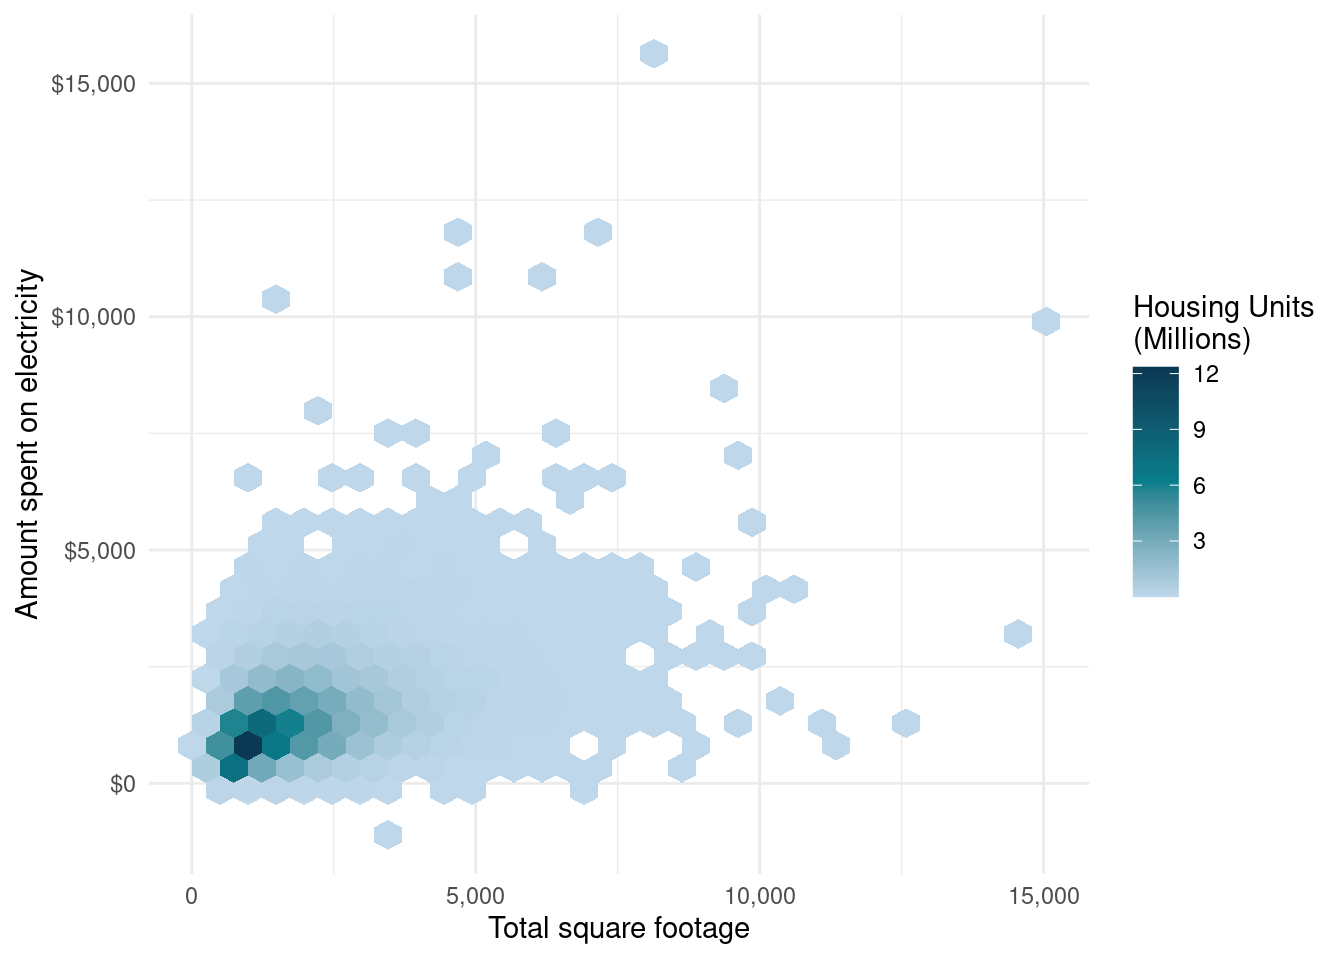
\includegraphics{bookdown_files/figure-latex/model-plot-sf-elbill-1} \caption{Relationship between square footage and dollars spent on electricity, RECS 2020}\label{fig:model-plot-sf-elbill}
\end{figure}

Given that the plot shows a potential increasing relationship between square footage and electricity expenditure, fitting a model will allow us to determine if the relationship is statistically significant. The model is fit below with electricity expenditure as the outcome.

\begin{Shaded}
\begin{Highlighting}[]
\NormalTok{m\_electric\_sqft }\OtherTok{\textless{}{-}}\NormalTok{ recs\_des }\SpecialCharTok{\%\textgreater{}\%}
  \FunctionTok{svyglm}\NormalTok{(}
    \AttributeTok{design =}\NormalTok{ .,}
    \AttributeTok{formula =}\NormalTok{ DOLLAREL }\SpecialCharTok{\textasciitilde{}}\NormalTok{ TOTSQFT\_EN,}
    \AttributeTok{na.action =}\NormalTok{ na.omit}
\NormalTok{  )}
\end{Highlighting}
\end{Shaded}

\begin{Shaded}
\begin{Highlighting}[]
\FunctionTok{tidy}\NormalTok{(m\_electric\_sqft) }\SpecialCharTok{\%\textgreater{}\%}
  \FunctionTok{mutate}\NormalTok{(}\AttributeTok{p.value =} \FunctionTok{pretty\_p\_value}\NormalTok{(p.value)) }\SpecialCharTok{\%\textgreater{}\%}
  \FunctionTok{gt}\NormalTok{() }\SpecialCharTok{\%\textgreater{}\%}
  \FunctionTok{fmt\_number}\NormalTok{()}
\end{Highlighting}
\end{Shaded}



\begin{longtable}{lrrrl}
\caption{\label{tab:model-slr-examp-tab}Linear regression output predicting electricity expenditure given square footage, RECS 2020}\\
\toprule
term & estimate & std.error & statistic & p.value \\ 
\midrule\relax
(Intercept) & $836.72$ & $12.77$ & $65.51$ & <0.0001 \\ 
TOTSQFT\_EN & $0.30$ & $0.01$ & $41.67$ & <0.0001 \\ 
\bottomrule
\end{longtable}

In the output above, we can see the estimated coefficients (\texttt{estimate}), estimated standard errors of the coefficients (\texttt{std.error}), the t-statistic (\texttt{statistic}), and the p-value for each coefficient. In these results, we can say that, on average, for every additional square foot of house size, the electricity bill increases by 29.9 cents and that square footage is significantly associated with electricity expenditure (p-value\textless0.0001).

This is a very simple model, and there are likely many more factors related to electricity expenditure, including the type of cooling, number of appliances, location, and more. However, starting with one variable models can help researchers understand what potential relationships there are between variables before fitting more complex models. Often researchers start with known relationships before building models to determine what impact additional variables have on the model.

\hypertarget{example-2-linear-regression-with-multiple-variables-and-interactions}{%
\subsubsection*{Example 2: Linear Regression with Multiple Variables and Interactions}\label{example-2-linear-regression-with-multiple-variables-and-interactions}}


In the following example, a model is fit to predict electricity expenditure, including Census region (factor/categorical), urbanicity (factor/categorical), square footage (double/numeric), and whether air-conditioning is used (logical/categorical) with all two-way interactions also included. In this example, we are choosing to fit this model without an intercept (using \texttt{-1} in the formula). This will result in an intercept estimate for each region instead of a single intercept for all data.

\begin{Shaded}
\begin{Highlighting}[]
\NormalTok{m\_electric\_multi }\OtherTok{\textless{}{-}}\NormalTok{ recs\_des }\SpecialCharTok{\%\textgreater{}\%}
  \FunctionTok{svyglm}\NormalTok{(}
    \AttributeTok{design =}\NormalTok{ .,}
    \AttributeTok{formula =}\NormalTok{ DOLLAREL }\SpecialCharTok{\textasciitilde{}}\NormalTok{ (Region }\SpecialCharTok{+}\NormalTok{ Urbanicity }\SpecialCharTok{+}\NormalTok{ TOTSQFT\_EN }\SpecialCharTok{+}\NormalTok{ ACUsed)}\SpecialCharTok{\^{}}\DecValTok{2} \SpecialCharTok{{-}} \DecValTok{1}\NormalTok{,}
    \AttributeTok{na.action =}\NormalTok{ na.omit}
\NormalTok{  )}
\end{Highlighting}
\end{Shaded}

\begin{Shaded}
\begin{Highlighting}[]
\FunctionTok{tidy}\NormalTok{(m\_electric\_multi) }\SpecialCharTok{\%\textgreater{}\%}
  \FunctionTok{mutate}\NormalTok{(}\AttributeTok{p.value =} \FunctionTok{pretty\_p\_value}\NormalTok{(p.value)) }\SpecialCharTok{\%\textgreater{}\%}
  \FunctionTok{gt}\NormalTok{() }\SpecialCharTok{\%\textgreater{}\%}
  \FunctionTok{fmt\_number}\NormalTok{()}
\end{Highlighting}
\end{Shaded}



\begin{longtable}{lrrrl}
\caption{\label{tab:model-lmr-examp-tab}Linear regression output predicting electricity expenditure given region, urbanicity, square footage, air conditioning usage, and one-way interactions, RECS 2020}\\
\toprule
term & estimate & std.error & statistic & p.value \\ 
\midrule
RegionNortheast & $543.73$ & $56.57$ & $9.61$ & <0.0001 \\ 
RegionMidwest & $702.16$ & $78.12$ & $8.99$ & <0.0001 \\ 
RegionSouth & $938.74$ & $46.99$ & $19.98$ & <0.0001 \\ 
RegionWest & $603.27$ & $36.31$ & $16.61$ & <0.0001 \\ 
UrbanicityUrban Cluster & $73.03$ & $81.50$ & $0.90$ & 0.3764 \\ 
UrbanicityRural & $204.13$ & $80.69$ & $2.53$ & 0.0161 \\ 
TOTSQFT\_EN & $0.24$ & $0.03$ & $8.65$ & <0.0001 \\ 
ACUsedTRUE & $252.06$ & $54.05$ & $4.66$ & <0.0001 \\ 
RegionMidwest:UrbanicityUrban Cluster & $183.06$ & $82.38$ & $2.22$ & 0.0328 \\ 
RegionSouth:UrbanicityUrban Cluster & $152.56$ & $76.03$ & $2.01$ & 0.0526 \\ 
RegionWest:UrbanicityUrban Cluster & $98.02$ & $75.16$ & $1.30$ & 0.2007 \\ 
RegionMidwest:UrbanicityRural & $312.83$ & $50.88$ & $6.15$ & <0.0001 \\ 
RegionSouth:UrbanicityRural & $220.00$ & $55.00$ & $4.00$ & 0.0003 \\ 
RegionWest:UrbanicityRural & $180.97$ & $58.70$ & $3.08$ & 0.0040 \\ 
RegionMidwest:TOTSQFT\_EN & $-0.05$ & $0.02$ & $-2.09$ & 0.0441 \\ 
RegionSouth:TOTSQFT\_EN & $0.00$ & $0.03$ & $0.11$ & 0.9109 \\ 
RegionWest:TOTSQFT\_EN & $-0.03$ & $0.03$ & $-1.00$ & 0.3254 \\ 
RegionMidwest:ACUsedTRUE & $-292.97$ & $60.24$ & $-4.86$ & <0.0001 \\ 
RegionSouth:ACUsedTRUE & $-294.07$ & $57.44$ & $-5.12$ & <0.0001 \\ 
RegionWest:ACUsedTRUE & $-77.68$ & $47.05$ & $-1.65$ & 0.1076 \\ 
UrbanicityUrban Cluster:TOTSQFT\_EN & $-0.04$ & $0.02$ & $-1.63$ & 0.1112 \\ 
UrbanicityRural:TOTSQFT\_EN & $-0.06$ & $0.02$ & $-2.60$ & 0.0137 \\ 
UrbanicityUrban Cluster:ACUsedTRUE & $-130.23$ & $60.30$ & $-2.16$ & 0.0377 \\ 
UrbanicityRural:ACUsedTRUE & $-33.80$ & $59.30$ & $-0.57$ & 0.5724 \\ 
TOTSQFT\_EN:ACUsedTRUE & $0.08$ & $0.02$ & $3.48$ & 0.0014 \\ 
\bottomrule
\end{longtable}

As shown above, there are many terms in this model. To test whether coefficients for a term are different from zero, the function \texttt{regTermTest()} can be used. For example, in the above regression, we can test whether the interaction of region and urbanicity is significant as follows:

\begin{Shaded}
\begin{Highlighting}[]
\NormalTok{urb\_reg\_test }\OtherTok{\textless{}{-}} \FunctionTok{regTermTest}\NormalTok{(m\_electric\_multi, }\SpecialCharTok{\textasciitilde{}}\NormalTok{ Urbanicity}\SpecialCharTok{:}\NormalTok{Region)}
\NormalTok{urb\_reg\_test}
\end{Highlighting}
\end{Shaded}

\begin{verbatim}
## Wald test for Urbanicity:Region
##  in svyglm(design = ., formula = DOLLAREL ~ (Region + Urbanicity + 
##     TOTSQFT_EN + ACUsed)^2 - 1, na.action = na.omit)
## F =  6.851  on  6  and  35  df: p= 7.2e-05
\end{verbatim}

This output indicates there is a significant interaction between urbanicity and region (p-value=\textless0.0001).

To examine the predictions, residuals, and more from the model, the function \texttt{augment()} from \{broom\} can be used. The \texttt{augment()} function will return a tibble with the independent and dependent variables and other fit statistics. The \texttt{augment()} function has not been specifically written for objects of class \texttt{svyglm}, and as such, a warning will be displayed indicating this at this time. As it was not written exactly for this class of objects, a little tweaking needs to be done after using \texttt{augment()}. To obtain the standard error of the predicted values (\texttt{.se.fit}) we need to use the \texttt{attr()} function on the predicted values (\texttt{.fitted}) created by \texttt{augment()}. Additionally, the predicted values created are outputted as a \texttt{svrep} type of data. If we want to plot the predicted values, we need to use \texttt{as.numeric()} to get the predicted values into a numeric format to work with. However, it is important to note that this adjustment must be completed \textbf{after} the standard error adjustment.

\begin{Shaded}
\begin{Highlighting}[]
\NormalTok{fitstats }\OtherTok{\textless{}{-}}
  \FunctionTok{augment}\NormalTok{(m\_electric\_multi) }\SpecialCharTok{\%\textgreater{}\%}
  \FunctionTok{mutate}\NormalTok{(}
    \AttributeTok{.se.fit =} \FunctionTok{sqrt}\NormalTok{(}\FunctionTok{attr}\NormalTok{(.fitted, }\StringTok{"var"}\NormalTok{)),}
    \AttributeTok{.fitted =} \FunctionTok{as.numeric}\NormalTok{(.fitted)}
\NormalTok{  )}

\NormalTok{fitstats}
\end{Highlighting}
\end{Shaded}

\begin{verbatim}
## # A tibble: 18,496 x 13
##    DOLLAREL Region    Urbanicity   TOTSQFT_EN ACUsed `(weights)` .fitted
##       <dbl> <fct>     <fct>             <dbl> <lgl>        <dbl>   <dbl>
##  1    1955. West      Urban Area         2100 TRUE         0.492   1397.
##  2     713. South     Urban Area          590 TRUE         1.35    1090.
##  3     335. West      Urban Area          900 TRUE         0.849   1043.
##  4    1425. South     Urban Area         2100 TRUE         0.793   1584.
##  5    1087  Northeast Urban Area          800 TRUE         1.49    1055.
##  6    1896. South     Urban Area         4520 TRUE         1.09    2375.
##  7    1418. South     Urban Area         2100 TRUE         0.851   1584.
##  8    1237. South     Urban Clust~        900 FALSE        1.45    1349.
##  9     538. South     Urban Area          750 TRUE         0.185   1142.
## 10     625. West      Urban Area          760 TRUE         1.06    1002.
## # i 18,486 more rows
## # i 6 more variables: .resid <dbl>, .hat <dbl>, .sigma <dbl>,
## #   .cooksd <dbl>, .std.resid <dbl>, .se.fit <dbl>
\end{verbatim}

These results can then be used in a variety of ways, including examining residual plots as illustrated in the code below and Figure \ref{fig:model-aug-examp-plot}. In the residual plot, we look for any patterns in the data. If we do see patterns, this may indicate a violation of the heteroscedasticity assumption and the standard errors of the coefficients may be incorrect. In Figure \ref{fig:model-aug-examp-plot}, we do not see a strong pattern indicating that our assumption of heteroscedasticity may hold.

\begin{Shaded}
\begin{Highlighting}[]
\NormalTok{fitstats }\SpecialCharTok{\%\textgreater{}\%}
  \FunctionTok{ggplot}\NormalTok{(}\FunctionTok{aes}\NormalTok{(}\AttributeTok{x =}\NormalTok{ .fitted, .resid)) }\SpecialCharTok{+}
  \FunctionTok{geom\_point}\NormalTok{() }\SpecialCharTok{+}
  \FunctionTok{geom\_hline}\NormalTok{(}\AttributeTok{yintercept =} \DecValTok{0}\NormalTok{, }\AttributeTok{color =} \StringTok{"red"}\NormalTok{) }\SpecialCharTok{+}
  \FunctionTok{theme\_minimal}\NormalTok{() }\SpecialCharTok{+}
  \FunctionTok{xlab}\NormalTok{(}\StringTok{"Fitted value of electricity cost"}\NormalTok{) }\SpecialCharTok{+}
  \FunctionTok{ylab}\NormalTok{(}\StringTok{"Residual of model"}\NormalTok{) }\SpecialCharTok{+}
  \FunctionTok{scale\_y\_continuous}\NormalTok{(}\AttributeTok{labels =}\NormalTok{ scales}\SpecialCharTok{::}\FunctionTok{dollar\_format}\NormalTok{()) }\SpecialCharTok{+}
  \FunctionTok{scale\_x\_continuous}\NormalTok{(}\AttributeTok{labels =}\NormalTok{ scales}\SpecialCharTok{::}\FunctionTok{dollar\_format}\NormalTok{())}
\end{Highlighting}
\end{Shaded}

\begin{figure}
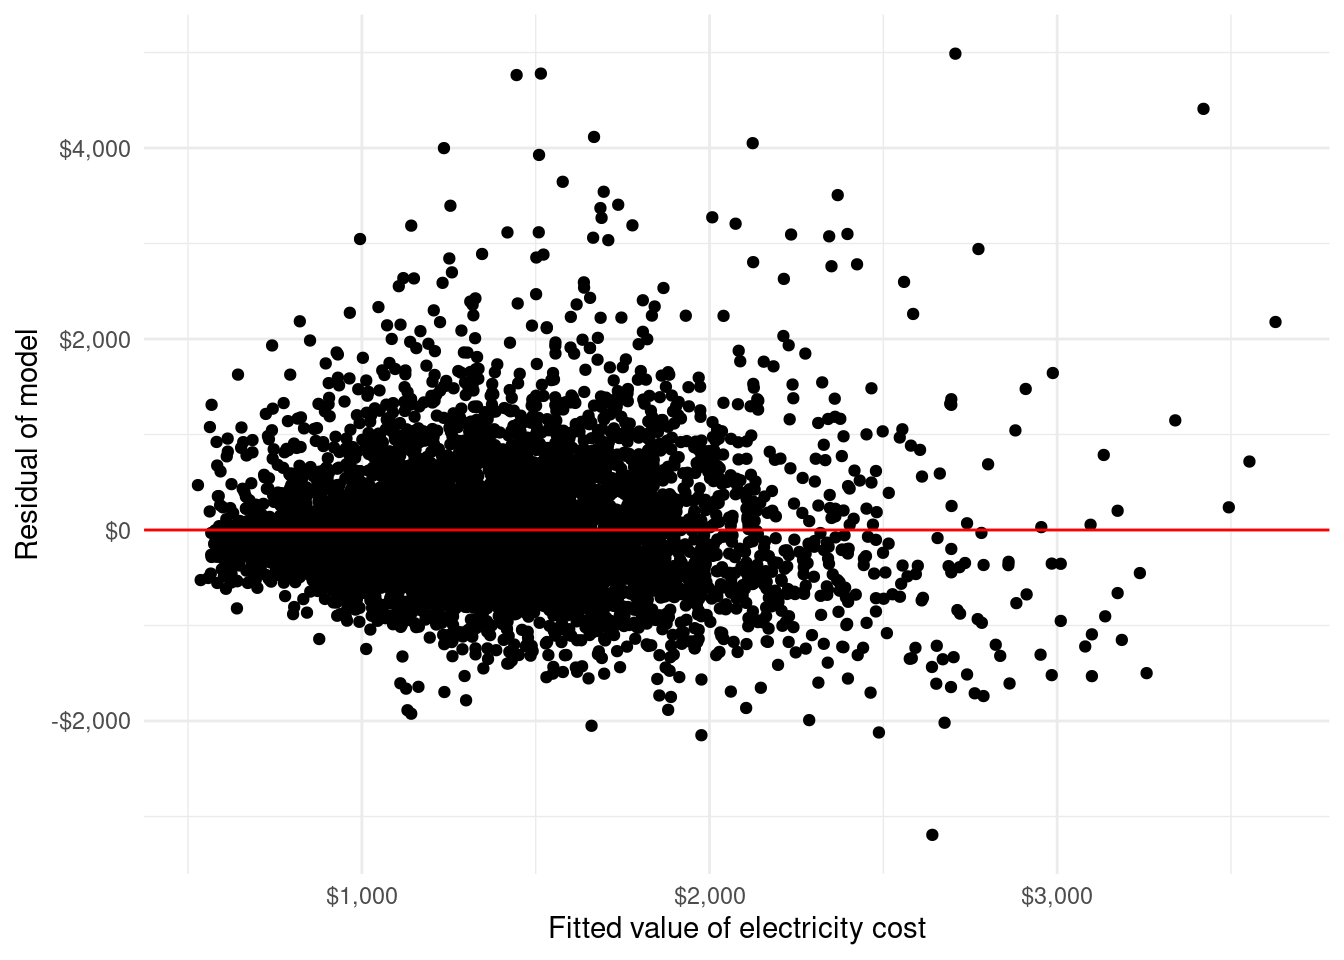
\includegraphics{bookdown_files/figure-latex/model-aug-examp-plot-1} \caption{Residual plot of electric cost model with covariates Region, Urbanicity, TOTSQFT\_EN, and ACUsed}\label{fig:model-aug-examp-plot}
\end{figure}

Additionally, \texttt{augment()} can be used to predict outcomes for data not used in modeling. Perhaps, we would like to predict the energy expenditure for a home in an urban area in the south that uses air-conditioning and is 2,500 square feet. To do this, we first make a tibble including that additional data and then use the \texttt{newdata} argument in the \texttt{augment()} function. As before, to obtain the standard error of the predicted values we need to use the \texttt{attr()} function.

\begin{Shaded}
\begin{Highlighting}[]
\NormalTok{add\_data }\OtherTok{\textless{}{-}}\NormalTok{ recs\_2020 }\SpecialCharTok{\%\textgreater{}\%}
  \FunctionTok{select}\NormalTok{(}
\NormalTok{    DOEID, Region, Urbanicity,}
\NormalTok{    TOTSQFT\_EN, ACUsed,}
\NormalTok{    DOLLAREL}
\NormalTok{  ) }\SpecialCharTok{\%\textgreater{}\%}
  \FunctionTok{rbind}\NormalTok{(}
    \FunctionTok{tibble}\NormalTok{(}
      \AttributeTok{DOEID =} \ConstantTok{NA}\NormalTok{,}
      \AttributeTok{Region =} \StringTok{"South"}\NormalTok{,}
      \AttributeTok{Urbanicity =} \StringTok{"Urban Area"}\NormalTok{,}
      \AttributeTok{TOTSQFT\_EN =} \DecValTok{2500}\NormalTok{,}
      \AttributeTok{ACUsed =} \ConstantTok{TRUE}\NormalTok{,}
      \AttributeTok{DOLLAREL =} \ConstantTok{NA}
\NormalTok{    )}
\NormalTok{  ) }\SpecialCharTok{\%\textgreater{}\%}
  \FunctionTok{tail}\NormalTok{(}\DecValTok{1}\NormalTok{)}

\NormalTok{pred\_data }\OtherTok{\textless{}{-}} \FunctionTok{augment}\NormalTok{(m\_electric\_multi, }\AttributeTok{newdata =}\NormalTok{ add\_data) }\SpecialCharTok{\%\textgreater{}\%}
  \FunctionTok{mutate}\NormalTok{(}
    \AttributeTok{.se.fit =} \FunctionTok{sqrt}\NormalTok{(}\FunctionTok{attr}\NormalTok{(.fitted, }\StringTok{"var"}\NormalTok{)),}
    \AttributeTok{.fitted =} \FunctionTok{as.numeric}\NormalTok{(.fitted)}
\NormalTok{  )}

\NormalTok{pred\_data}
\end{Highlighting}
\end{Shaded}

\begin{verbatim}
## # A tibble: 1 x 8
##   DOEID Region Urbanicity TOTSQFT_EN ACUsed DOLLAREL .fitted .se.fit
##   <dbl> <fct>  <fct>           <dbl> <lgl>     <dbl>   <dbl>   <dbl>
## 1    NA South  Urban Area       2500 TRUE         NA   1715.    22.6
\end{verbatim}

In the above example, it is predicted that the energy expenditure would be \$1,715.

\hypertarget{logistic-regression}{%
\section{Logistic Regression}\label{logistic-regression}}

Logistic regression is used to model binary outcomes such as whether or not someone voted. There are several instances where an outcome may not be originally binary but is collapsed into being binary. For example, given that gender is often asked in surveys with multiple response options and not a binary scale, many researchers now code gender in logistic modeling as cis-male compared to not cis-male. We could also convert a 4-point likert scale that has levels of ``Strongly Agree'', ``Agree'', ``Disagree'', and ``Strongly Disagree'' to group the agreement levels into one group and disagreement levels into a second group.

Logistic regression is a specific case of the generalized linear model (GLM). A GLM uses a link function to link the response variable to the linear model. If we tried to use a normal linear regression with a binary outcome, many assumptions are not held - namely the response is not continuous. Logistic regression allows us to link a linear model between the covariates and a propensity of an outcome. In logistic regression, the link model is the logit function. Specifically, the model is specified as follows:

\[ y_i \sim \text{Bernoulli}(\pi_i)\]

\begin{equation}
\log \left(\frac{\pi_i}{1-\pi_i} \right)=\beta_0 +\sum_{i=1}^n \beta_i x_i
\label{eq:logoddlin}
\end{equation}

which can be re-expressed as

\[ \pi_i=\frac{\exp \left(\beta_0 +\sum_{i=1}^n \beta_i x_i \right)}{1+\exp \left(\beta_0 +\sum_{i=1}^n \beta_i x_i \right)}.\] where \(y_i\) is the outcome, \(\beta_0\) is an intercept, and \(x_1, \cdots, x_n\) are the predictors with \(\beta_1, \cdots, \beta_n\) as the associated coefficients.

The Bernoulli distribution is a distribution which has an outcome of 0 or 1 given some probability (\(\pi_i\)) in this case and we model \(\pi_i\) as a function of the covariates \(x_i\) using this logit link.

Assumptions in logistic regression using survey data include:

\begin{itemize}
\tightlist
\item
  The outcome variable has two levels
\item
  There is a linear relationship between the independent variables and the log odds (Equation \eqref{eq:logoddlin})
\item
  The residuals are homoscedastic, that is, the error term is the same across all values of independent variables
\end{itemize}

\hypertarget{syntax-8}{%
\subsection{Syntax}\label{syntax-8}}

The syntax for logistic regression is as follows:

\begin{Shaded}
\begin{Highlighting}[]
\NormalTok{des\_obj }\SpecialCharTok{\%\textgreater{}\%}
  \FunctionTok{svyglm}\NormalTok{(}
    \AttributeTok{formula =}\NormalTok{ outcomevar }\SpecialCharTok{\textasciitilde{}}\NormalTok{ x1 }\SpecialCharTok{+}\NormalTok{ x2 }\SpecialCharTok{+}\NormalTok{ x3,}
    \AttributeTok{design =}\NormalTok{ .,}
    \AttributeTok{na.action =}\NormalTok{ na.omit,}
    \AttributeTok{df.resid =} \ConstantTok{NULL}\NormalTok{,}
    \AttributeTok{family =}\NormalTok{ quasibinomial}
\NormalTok{  )}
\end{Highlighting}
\end{Shaded}

The arguments are:

\begin{itemize}
\tightlist
\item
  \texttt{formula}: Formula in the form of \texttt{y\textasciitilde{}x}
\item
  \texttt{design}: a \texttt{tbl\_svy} object created by \texttt{as\_survey}
\item
  \texttt{na.action}: handling of missing data
\item
  \texttt{df.resid}: degrees of freedom for Wald tests (optional) - defaults to using \texttt{degf(design)-p} where \(p\) is the rank of the design matrix
\item
  \texttt{family}: the error distribution/link function to be used in the model
\end{itemize}

Note \texttt{svyglm()} is the same function used in both ANOVA and normal linear regression. However, we've added the link function quasibinomial. While we can use the binomial link function, it is recommended to use the quasibinomial as our weights may not be integers, and the quasibinomial also allows for overdispersion \citep{mccullagh1989binary, lumley2010complex, rcore}. The quasibinomial family has a default logit link which is what is specified in the equations above. When specifying the outcome variable, it will likely be specified in one of three ways with survey data:

\begin{itemize}
\tightlist
\item
  A two level factor variable where the first level of the factor indicates a ``failure'' and the second level indicates a ``success''
\item
  A numeric variable which is 1 or 0 where 1 indicates a success
\item
  A logical variable where TRUE indicates a success
\end{itemize}

\hypertarget{examples-8}{%
\subsection{Examples}\label{examples-8}}

\hypertarget{example-1-logistic-regression-with-single-variable}{%
\subsubsection*{Example 1: Logistic Regression with Single Variable}\label{example-1-logistic-regression-with-single-variable}}


In the following example, the ANES data is used, and we are modeling whether someone usually has trust in the government\footnote{Question: How often can you trust the federal government in Washington to do what is right?} by who someone voted for president in 2020. As a reminder, the leading candidates were Biden and Trump though people could vote for someone else not in the Democratic or Republican parties. Those votes are all grouped into an ``Other'' category. We first create a binary outcome for trusting in the government by collapsing ``Always'' and ``Most of the time'' into a single factor level, and the other response options (``About half the time'', ``Some of the time'', and ``Never'') into a second factor level. Next, a scatter plot of the raw data is not useful as it is all 0 and 1 outcomes, so instead, we plot a summary of the data.

\begin{Shaded}
\begin{Highlighting}[]
\NormalTok{anes\_des\_der }\OtherTok{\textless{}{-}}\NormalTok{ anes\_des }\SpecialCharTok{\%\textgreater{}\%}
  \FunctionTok{mutate}\NormalTok{(}\AttributeTok{TrustGovernmentUsually =} \FunctionTok{case\_when}\NormalTok{(}
    \FunctionTok{is.na}\NormalTok{(TrustGovernment) }\SpecialCharTok{\textasciitilde{}} \ConstantTok{NA}\NormalTok{,}
    \ConstantTok{TRUE} \SpecialCharTok{\textasciitilde{}}\NormalTok{ TrustGovernment }\SpecialCharTok{\%in\%} \FunctionTok{c}\NormalTok{(}\StringTok{"Always"}\NormalTok{, }\StringTok{"Most of the time"}\NormalTok{)}
\NormalTok{  ))}

\NormalTok{anes\_des\_der }\SpecialCharTok{\%\textgreater{}\%}
  \FunctionTok{group\_by}\NormalTok{(VotedPres2020\_selection) }\SpecialCharTok{\%\textgreater{}\%}
  \FunctionTok{summarize}\NormalTok{(}
    \AttributeTok{pct\_trust =} \FunctionTok{survey\_mean}\NormalTok{(TrustGovernmentUsually,}
      \AttributeTok{na.rm =} \ConstantTok{TRUE}\NormalTok{,}
      \AttributeTok{proportion =} \ConstantTok{TRUE}\NormalTok{,}
      \AttributeTok{vartype =} \StringTok{"ci"}
\NormalTok{    ),}
    \AttributeTok{.groups =} \StringTok{"drop"}
\NormalTok{  ) }\SpecialCharTok{\%\textgreater{}\%}
  \FunctionTok{filter}\NormalTok{(}\FunctionTok{complete.cases}\NormalTok{(.)) }\SpecialCharTok{\%\textgreater{}\%}
  \FunctionTok{ggplot}\NormalTok{(}\FunctionTok{aes}\NormalTok{(}
    \AttributeTok{x =}\NormalTok{ VotedPres2020\_selection, }\AttributeTok{y =}\NormalTok{ pct\_trust,}
    \AttributeTok{fill =}\NormalTok{ VotedPres2020\_selection}
\NormalTok{  )) }\SpecialCharTok{+}
  \FunctionTok{geom\_bar}\NormalTok{(}\AttributeTok{stat =} \StringTok{"identity"}\NormalTok{) }\SpecialCharTok{+}
  \FunctionTok{geom\_errorbar}\NormalTok{(}\FunctionTok{aes}\NormalTok{(}\AttributeTok{ymin =}\NormalTok{ pct\_trust\_low, }\AttributeTok{ymax =}\NormalTok{ pct\_trust\_upp),}
    \AttributeTok{width =}\NormalTok{ .}\DecValTok{2}
\NormalTok{  ) }\SpecialCharTok{+}
  \FunctionTok{scale\_fill\_manual}\NormalTok{(}\AttributeTok{values =} \FunctionTok{c}\NormalTok{(}\StringTok{"\#0b3954"}\NormalTok{, }\StringTok{"\#bfd7ea"}\NormalTok{, }\StringTok{"\#8d6b94"}\NormalTok{)) }\SpecialCharTok{+}
  \FunctionTok{xlab}\NormalTok{(}\StringTok{"Election choice (2020)"}\NormalTok{) }\SpecialCharTok{+}
  \FunctionTok{ylab}\NormalTok{(}\StringTok{"Usually trust the government"}\NormalTok{) }\SpecialCharTok{+}
  \FunctionTok{scale\_y\_continuous}\NormalTok{(}\AttributeTok{labels =}\NormalTok{ scales}\SpecialCharTok{::}\NormalTok{percent) }\SpecialCharTok{+}
  \FunctionTok{guides}\NormalTok{(}\AttributeTok{fill =} \StringTok{"none"}\NormalTok{) }\SpecialCharTok{+}
  \FunctionTok{theme\_minimal}\NormalTok{()}
\end{Highlighting}
\end{Shaded}

\begin{figure}
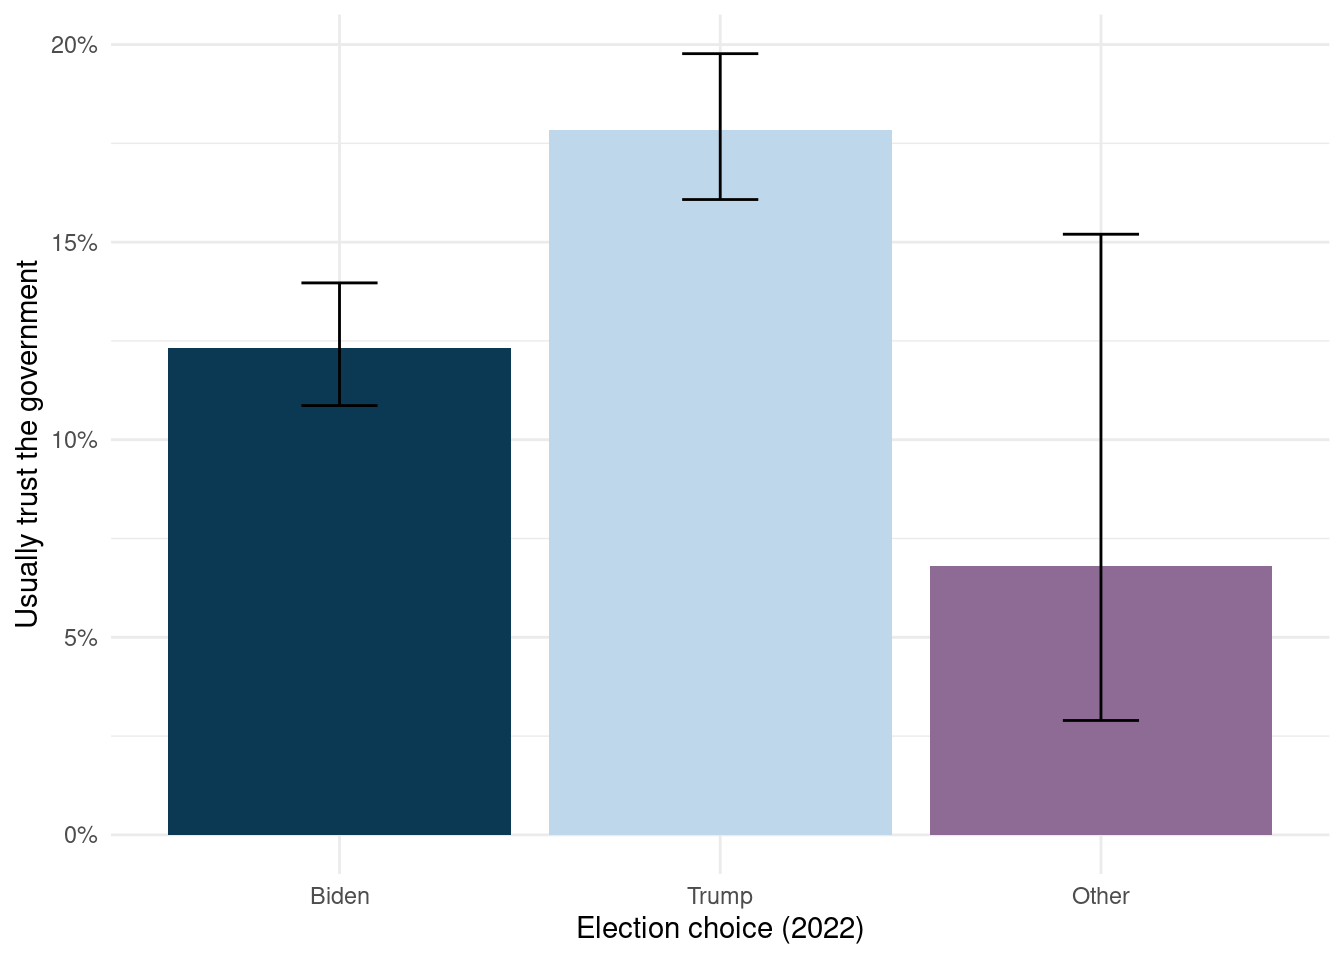
\includegraphics{bookdown_files/figure-latex/model-logisticexamp-plot-1} \caption{Relationship between candidate selection and trust in government, ANES 2020}\label{fig:model-logisticexamp-plot}
\end{figure}

By looking at Figure \ref{fig:model-logisticexamp-plot} it appears that people who voted for Trump are more likely to say that they usually have trust in the government compared to those who voted for Biden and Other candidates. To determine if this insight is accurate, we next we fit the model.

\begin{Shaded}
\begin{Highlighting}[]
\NormalTok{logistic\_trust\_vote }\OtherTok{\textless{}{-}}\NormalTok{ anes\_des\_der }\SpecialCharTok{\%\textgreater{}\%}
  \FunctionTok{svyglm}\NormalTok{(}
    \AttributeTok{design =}\NormalTok{ .,}
    \AttributeTok{formula =}\NormalTok{ TrustGovernmentUsually }\SpecialCharTok{\textasciitilde{}}\NormalTok{ VotedPres2020\_selection,}
    \AttributeTok{family =}\NormalTok{ quasibinomial}
\NormalTok{  )}
\end{Highlighting}
\end{Shaded}

\begin{Shaded}
\begin{Highlighting}[]
\FunctionTok{tidy}\NormalTok{(logistic\_trust\_vote) }\SpecialCharTok{\%\textgreater{}\%}
  \FunctionTok{mutate}\NormalTok{(}\AttributeTok{p.value =} \FunctionTok{pretty\_p\_value}\NormalTok{(p.value)) }\SpecialCharTok{\%\textgreater{}\%}
  \FunctionTok{gt}\NormalTok{() }\SpecialCharTok{\%\textgreater{}\%}
  \FunctionTok{fmt\_number}\NormalTok{()}
\end{Highlighting}
\end{Shaded}



\begin{longtable}{lrrrl}
\caption{\label{tab:model-logisticexamp-tab}Logistic regression output predicting trust in government by presidential candidate selection, RECS 2020}\\
\toprule
term & estimate & std.error & statistic & p.value \\ 
\midrule\relax
(Intercept) & $-1.96$ & $0.07$ & $-27.45$ & <0.0001 \\ 
VotedPres2020\_selectionTrump & $0.43$ & $0.09$ & $4.72$ & <0.0001 \\ 
VotedPres2020\_selectionOther & $-0.65$ & $0.44$ & $-1.49$ & 0.1429 \\ 
\bottomrule
\end{longtable}

In the output above, we can see the estimated coefficients (\texttt{estimate}), estimated standard errors of the coefficients (\texttt{std.error}), the t-statistic (\texttt{statistic}), and the p-value for each coefficient. This output indicates that respondents who voted for Trump are 0.435 times more likely to usually have trust in the government compared to those who voted for Biden (the reference level).

Sometimes it is easier to talk about the odds instead of the likelihood. To do this, we need to exponentiate the coefficients. We can use the same \texttt{tidy()} function, but include the argument \texttt{exponentiate\ =\ TRUE} to see the odds.

\begin{Shaded}
\begin{Highlighting}[]
\FunctionTok{tidy}\NormalTok{(logistic\_trust\_vote, }\AttributeTok{exponentiate =} \ConstantTok{TRUE}\NormalTok{) }\SpecialCharTok{\%\textgreater{}\%}
  \FunctionTok{select}\NormalTok{(term, estimate) }\SpecialCharTok{\%\textgreater{}\%}
  \FunctionTok{gt}\NormalTok{() }\SpecialCharTok{\%\textgreater{}\%}
  \FunctionTok{fmt\_number}\NormalTok{()}
\end{Highlighting}
\end{Shaded}



\begin{longtable}{lr}
\caption{\label{tab:model-logisticexamp-model-odds-tab}Logistic regression predicting trust in government by presidential candidate selection with exponentiated coefficients (odds), RECS 2020}\\
\toprule
term & estimate \\ 
\midrule\relax
(Intercept) & $0.14$ \\ 
VotedPres2020\_selectionTrump & $1.54$ \\ 
VotedPres2020\_selectionOther & $0.52$ \\ 
\bottomrule
\end{longtable}

We can interpret this as saying that the odds of usually trusting the government for someone who voted for Trump is 154\% as likely to trust the government compared to a person who voted for Biden (the reference level). In comparison, a person who voted for neither Biden nor Trump is 52\% as likely to trust the government as someone who voted for Biden.

As with linear regression, the \texttt{augment()} can be used to predict values. By default, the prediction is the link function and not the probability. To predict the probability, add an argument of \texttt{type.predict="response"} as demonstrated below:

\begin{Shaded}
\begin{Highlighting}[]
\NormalTok{logistic\_trust\_vote }\SpecialCharTok{\%\textgreater{}\%}
  \FunctionTok{augment}\NormalTok{(}\AttributeTok{type.predict =} \StringTok{"response"}\NormalTok{) }\SpecialCharTok{\%\textgreater{}\%}
  \FunctionTok{mutate}\NormalTok{(}
    \AttributeTok{.se.fit =} \FunctionTok{sqrt}\NormalTok{(}\FunctionTok{attr}\NormalTok{(.fitted, }\StringTok{"var"}\NormalTok{)),}
    \AttributeTok{.fitted =} \FunctionTok{as.numeric}\NormalTok{(.fitted)}
\NormalTok{  ) }\SpecialCharTok{\%\textgreater{}\%}
  \FunctionTok{select}\NormalTok{(}
\NormalTok{    TrustGovernmentUsually,}
\NormalTok{    VotedPres2020\_selection,}
\NormalTok{    .fitted,}
\NormalTok{    .se.fit}
\NormalTok{  )}
\end{Highlighting}
\end{Shaded}

\begin{verbatim}
## # A tibble: 6,212 x 4
##    TrustGovernmentUsually VotedPres2020_selection .fitted .se.fit
##    <lgl>                  <fct>                     <dbl>   <dbl>
##  1 FALSE                  Other                    0.0681 0.0279 
##  2 FALSE                  Biden                    0.123  0.00772
##  3 FALSE                  Biden                    0.123  0.00772
##  4 FALSE                  Trump                    0.178  0.00919
##  5 FALSE                  Biden                    0.123  0.00772
##  6 FALSE                  Trump                    0.178  0.00919
##  7 FALSE                  Biden                    0.123  0.00772
##  8 FALSE                  Biden                    0.123  0.00772
##  9 TRUE                   Biden                    0.123  0.00772
## 10 FALSE                  Biden                    0.123  0.00772
## # i 6,202 more rows
\end{verbatim}

\hypertarget{example-2-interaction-effects}{%
\subsubsection*{Example 2: Interaction Effects}\label{example-2-interaction-effects}}


Let's look at another example with interaction effects. If we're interested in understanding the demographics of people who voted for Biden among all voters in 2020, we could include \texttt{EarlyVote2020} and \texttt{Gender} in our model.

First we need to subset the data to 2020 voters and then create an indicator for voted for Biden.

\begin{Shaded}
\begin{Highlighting}[]
\NormalTok{anes\_des\_ind }\OtherTok{\textless{}{-}}\NormalTok{ anes\_des }\SpecialCharTok{\%\textgreater{}\%}
  \FunctionTok{filter}\NormalTok{(}\SpecialCharTok{!}\FunctionTok{is.na}\NormalTok{(VotedPres2020\_selection)) }\SpecialCharTok{\%\textgreater{}\%}
  \FunctionTok{mutate}\NormalTok{(}\AttributeTok{VoteBiden =} \FunctionTok{case\_when}\NormalTok{(}
\NormalTok{    VotedPres2020\_selection }\SpecialCharTok{==} \StringTok{"Biden"} \SpecialCharTok{\textasciitilde{}} \DecValTok{1}\NormalTok{,}
    \ConstantTok{TRUE} \SpecialCharTok{\textasciitilde{}} \DecValTok{0}
\NormalTok{  ))}
\end{Highlighting}
\end{Shaded}

Let's first look at the main effects of gender and early voting behavior.

\begin{Shaded}
\begin{Highlighting}[]
\NormalTok{log\_biden\_main }\OtherTok{\textless{}{-}}\NormalTok{ anes\_des\_ind }\SpecialCharTok{\%\textgreater{}\%}
  \FunctionTok{mutate}\NormalTok{(}\AttributeTok{EarlyVote2020 =} \FunctionTok{fct\_relevel}\NormalTok{(EarlyVote2020, }\StringTok{"No"}\NormalTok{, }\AttributeTok{after =} \DecValTok{0}\NormalTok{)) }\SpecialCharTok{\%\textgreater{}\%}
  \FunctionTok{svyglm}\NormalTok{(}
    \AttributeTok{design =}\NormalTok{ .,}
    \AttributeTok{formula =}\NormalTok{ VoteBiden }\SpecialCharTok{\textasciitilde{}}\NormalTok{ EarlyVote2020 }\SpecialCharTok{+}\NormalTok{ Gender,}
    \AttributeTok{family =}\NormalTok{ quasibinomial}
\NormalTok{  )}
\end{Highlighting}
\end{Shaded}

\begin{Shaded}
\begin{Highlighting}[]
\FunctionTok{tidy}\NormalTok{(log\_biden\_main) }\SpecialCharTok{\%\textgreater{}\%}
  \FunctionTok{mutate}\NormalTok{(}\AttributeTok{p.value =} \FunctionTok{pretty\_p\_value}\NormalTok{(p.value)) }\SpecialCharTok{\%\textgreater{}\%}
  \FunctionTok{gt}\NormalTok{() }\SpecialCharTok{\%\textgreater{}\%}
  \FunctionTok{fmt\_number}\NormalTok{()}
\end{Highlighting}
\end{Shaded}



\begin{longtable}{lrrrr}
\caption{\label{tab:model-logisticexamp-biden-main-tab}Logistic regression output for predicting voting for Biden given early voting behavior and gender - main effects only, RECS 2020}\\
\toprule
term & estimate & std.error & statistic & p.value \\ 
\midrule\relax
(Intercept) & $-0.31$ & $0.27$ & $-1.15$ & 0.2553 \\ 
EarlyVote2020Yes & $0.53$ & $0.35$ & $1.53$ & 0.1338 \\ 
GenderFemale & $0.96$ & $0.26$ & $3.73$ & 0.0005 \\ 
\bottomrule
\end{longtable}

This main effect model indicates that respondents with who early voted in 2020 are 0.528 (p-value=0.1338) times more likely to vote for Biden compared to respondents who did not early vote in the 2020 election (the reference level). We see that gender is also significant with females more likely to vote for Biden compared to males (p-value=0.0005).

It is possible that there is an interaction between gender and early voting behavior. To determine this we can create a model that includes the interaction effects:

\begin{Shaded}
\begin{Highlighting}[]
\NormalTok{log\_biden\_int }\OtherTok{\textless{}{-}}\NormalTok{ anes\_des\_ind }\SpecialCharTok{\%\textgreater{}\%}
  \FunctionTok{mutate}\NormalTok{(}\AttributeTok{EarlyVote2020 =} \FunctionTok{fct\_relevel}\NormalTok{(EarlyVote2020, }\StringTok{"No"}\NormalTok{, }\AttributeTok{after =} \DecValTok{0}\NormalTok{)) }\SpecialCharTok{\%\textgreater{}\%}
  \FunctionTok{svyglm}\NormalTok{(}
    \AttributeTok{design =}\NormalTok{ .,}
    \AttributeTok{formula =}\NormalTok{ VoteBiden }\SpecialCharTok{\textasciitilde{}}\NormalTok{ (EarlyVote2020 }\SpecialCharTok{+}\NormalTok{ Gender)}\SpecialCharTok{\^{}}\DecValTok{2}\NormalTok{,}
    \AttributeTok{family =}\NormalTok{ quasibinomial}
\NormalTok{  )}
\end{Highlighting}
\end{Shaded}

\begin{Shaded}
\begin{Highlighting}[]
\FunctionTok{tidy}\NormalTok{(log\_biden\_int) }\SpecialCharTok{\%\textgreater{}\%}
  \FunctionTok{mutate}\NormalTok{(}\AttributeTok{p.value =} \FunctionTok{pretty\_p\_value}\NormalTok{(p.value)) }\SpecialCharTok{\%\textgreater{}\%}
  \FunctionTok{gt}\NormalTok{() }\SpecialCharTok{\%\textgreater{}\%}
  \FunctionTok{fmt\_number}\NormalTok{()}
\end{Highlighting}
\end{Shaded}



\begin{longtable}{lrrrr}
\caption{\label{tab:model-logisticexamp-biden-int-tab}Logistic regression output for predicting voting for Biden given early voting behavior and gender - with interaction, RECS 2020}\\
\toprule
term & estimate & std.error & statistic & p.value \\ 
\midrule\relax
(Intercept) & $-0.20$ & $0.36$ & $-0.55$ & 0.5844 \\ 
EarlyVote2020Yes & $0.38$ & $0.47$ & $0.80$ & 0.4277 \\ 
GenderFemale & $0.76$ & $0.54$ & $1.42$ & 0.1625 \\ 
EarlyVote2020Yes:GenderFemale & $0.27$ & $0.60$ & $0.45$ & 0.6583 \\ 
\bottomrule
\end{longtable}

The results from the interaction model show that the interaction between early voting behavior and gender is significant. To better understand what this interaction means, we will want to plot the predicted probabilities with an interaction plot. Let's first obtain the predicted probabilities for each possible combination of variables using the \texttt{augment()} function.

\begin{Shaded}
\begin{Highlighting}[]
\NormalTok{log\_biden\_pred }\OtherTok{\textless{}{-}}\NormalTok{ log\_biden\_int }\SpecialCharTok{\%\textgreater{}\%}
  \FunctionTok{augment}\NormalTok{(}\AttributeTok{type.predict =} \StringTok{"response"}\NormalTok{) }\SpecialCharTok{\%\textgreater{}\%}
  \FunctionTok{mutate}\NormalTok{(}
    \AttributeTok{.se.fit =} \FunctionTok{sqrt}\NormalTok{(}\FunctionTok{attr}\NormalTok{(.fitted, }\StringTok{"var"}\NormalTok{)),}
    \AttributeTok{.fitted =} \FunctionTok{as.numeric}\NormalTok{(.fitted)}
\NormalTok{  ) }\SpecialCharTok{\%\textgreater{}\%}
  \FunctionTok{select}\NormalTok{(VoteBiden, EarlyVote2020, Gender, .fitted, .se.fit)}
\end{Highlighting}
\end{Shaded}

To create an interaction plot, the y-axis will be the predicted probabilities, and one of our x-variables will be on the x-axis and the other will be represented by multiple lines. Figure \ref{fig:model-logisticexamp-biden-plot} shows the interaction plot with gender on the x-axis and early voting behavior represented by the lines.

\begin{Shaded}
\begin{Highlighting}[]
\NormalTok{log\_biden\_pred }\SpecialCharTok{\%\textgreater{}\%}
  \FunctionTok{filter}\NormalTok{(VoteBiden }\SpecialCharTok{==} \DecValTok{1}\NormalTok{) }\SpecialCharTok{\%\textgreater{}\%}
  \FunctionTok{distinct}\NormalTok{() }\SpecialCharTok{\%\textgreater{}\%}
  \FunctionTok{arrange}\NormalTok{(Gender, EarlyVote2020) }\SpecialCharTok{\%\textgreater{}\%}
  \FunctionTok{mutate}\NormalTok{(}\AttributeTok{EarlyVote2020 =} \FunctionTok{fct\_reorder2}\NormalTok{(EarlyVote2020, Gender, .fitted)) }\SpecialCharTok{\%\textgreater{}\%}
  \FunctionTok{ggplot}\NormalTok{(}\FunctionTok{aes}\NormalTok{(}
    \AttributeTok{x =}\NormalTok{ Gender, }\AttributeTok{y =}\NormalTok{ .fitted, }\AttributeTok{group =}\NormalTok{ EarlyVote2020,}
    \AttributeTok{color =}\NormalTok{ EarlyVote2020, }\AttributeTok{linetype =}\NormalTok{ EarlyVote2020}
\NormalTok{  )) }\SpecialCharTok{+}
  \FunctionTok{geom\_line}\NormalTok{(}\AttributeTok{linewidth =} \FloatTok{1.1}\NormalTok{) }\SpecialCharTok{+}
  \FunctionTok{scale\_color\_manual}\NormalTok{(}\AttributeTok{values =}\NormalTok{ book\_colors[}\FunctionTok{c}\NormalTok{(}\DecValTok{2}\NormalTok{, }\DecValTok{4}\NormalTok{)]) }\SpecialCharTok{+}
  \FunctionTok{ylab}\NormalTok{(}\StringTok{"Predicted Probability of Voting for Biden"}\NormalTok{) }\SpecialCharTok{+}
  \FunctionTok{labs}\NormalTok{(}
    \AttributeTok{color =} \StringTok{"Voted Early"}\NormalTok{,}
    \AttributeTok{linetype =} \StringTok{"Voted Early"}
\NormalTok{  ) }\SpecialCharTok{+}
  \FunctionTok{coord\_cartesian}\NormalTok{(}\AttributeTok{ylim =} \FunctionTok{c}\NormalTok{(}\DecValTok{0}\NormalTok{, }\DecValTok{1}\NormalTok{)) }\SpecialCharTok{+}
  \FunctionTok{guides}\NormalTok{(}\AttributeTok{fill =} \StringTok{"none"}\NormalTok{) }\SpecialCharTok{+}
  \FunctionTok{theme\_minimal}\NormalTok{()}
\end{Highlighting}
\end{Shaded}

\begin{figure}
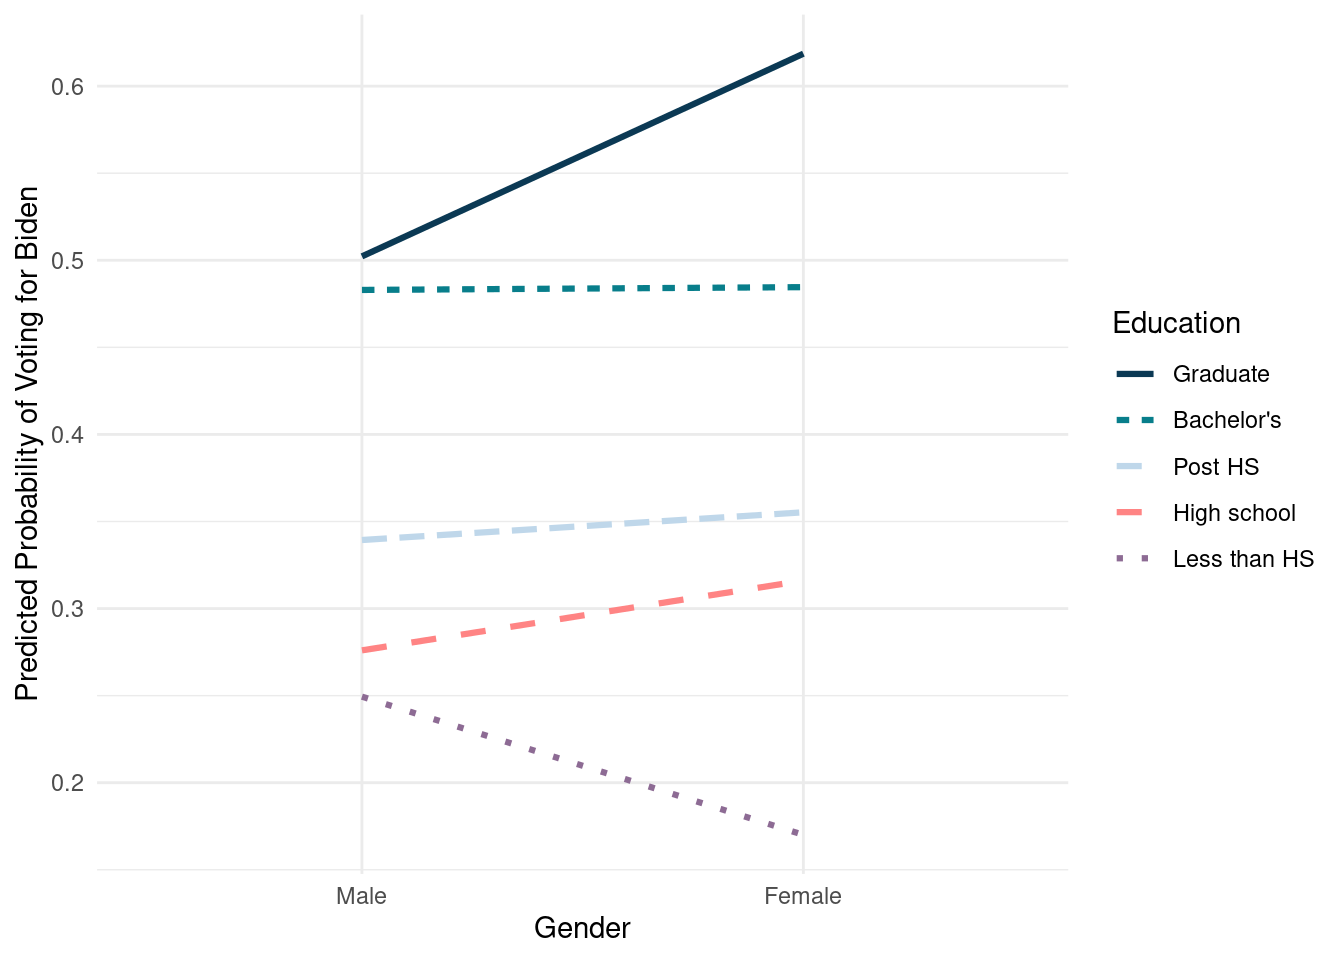
\includegraphics{bookdown_files/figure-latex/model-logisticexamp-biden-plot-1} \caption{Interaction Plot of Gender and Early Voting Predicting the Probability of Voting for Biden}\label{fig:model-logisticexamp-biden-plot}
\end{figure}

From this plot we can see that respondents who indicated a male gender had roughly the same probability of voting for Biden regardless of if they voted early or not. However, females who voted early were more likely to vote for Biden if they voted early than if they did not vote early.

Interactions in models can be difficult to understand from the coefficients alone. Using these interaction plots can help others understand the nuances of the results, and often can become even more helpful with more than two levels in a given factor (e.g., education or race/ethnicity).

\hypertarget{exercises-1}{%
\section{Exercises}\label{exercises-1}}

\begin{enumerate}
\def\labelenumi{\arabic{enumi}.}
\tightlist
\item
  The type of housing unit may have an impact on energy expenses. Using the RECS data, is there any relationship between housing unit type (\texttt{HousingUnitType}) and total energy expenditure (\texttt{TOTALDOL})? First, find the average energy expenditure by housing unit type as a descriptive analysis and then do the test. The reference level in the comparison should be the housing unit type that is most common.
\end{enumerate}

\begin{Shaded}
\begin{Highlighting}[]
\NormalTok{recs\_des }\SpecialCharTok{\%\textgreater{}\%}
  \FunctionTok{group\_by}\NormalTok{(HousingUnitType) }\SpecialCharTok{\%\textgreater{}\%}
  \FunctionTok{summarize}\NormalTok{(}
    \AttributeTok{Expense =} \FunctionTok{survey\_mean}\NormalTok{(TOTALDOL, }\AttributeTok{na.rm =} \ConstantTok{TRUE}\NormalTok{),}
    \AttributeTok{HUs =} \FunctionTok{survey\_total}\NormalTok{()}
\NormalTok{  ) }\SpecialCharTok{\%\textgreater{}\%}
  \FunctionTok{arrange}\NormalTok{(}\FunctionTok{desc}\NormalTok{(HUs))}
\end{Highlighting}
\end{Shaded}

\begin{verbatim}
## # A tibble: 5 x 5
##   HousingUnitType            Expense Expense_se       HUs       HUs_se
##   <fct>                        <dbl>      <dbl>     <dbl>        <dbl>
## 1 Single-family detached       2205.       9.36 77067692. 0.00000277  
## 2 Apartment: 5 or more units   1108.      13.7  22835862. 0.000000226 
## 3 Apartment: 2-4 Units         1407.      24.2   9341795. 0.119       
## 4 Single-family attached       1653.      22.3   7451177. 0.114       
## 5 Mobile home                  1773.      26.2   6832499. 0.0000000927
\end{verbatim}

\begin{Shaded}
\begin{Highlighting}[]
\NormalTok{exp\_unit\_out }\OtherTok{\textless{}{-}}\NormalTok{ recs\_des }\SpecialCharTok{\%\textgreater{}\%}
  \FunctionTok{mutate}\NormalTok{(}\AttributeTok{HousingUnitType =} \FunctionTok{fct\_infreq}\NormalTok{(HousingUnitType, NWEIGHT)) }\SpecialCharTok{\%\textgreater{}\%}
  \FunctionTok{svyglm}\NormalTok{(}
    \AttributeTok{design =}\NormalTok{ .,}
    \AttributeTok{formula =}\NormalTok{ TOTALDOL }\SpecialCharTok{\textasciitilde{}}\NormalTok{ HousingUnitType,}
    \AttributeTok{na.action =}\NormalTok{ na.omit}
\NormalTok{  )}

\FunctionTok{tidy}\NormalTok{(exp\_unit\_out)}
\end{Highlighting}
\end{Shaded}

\begin{verbatim}
## # A tibble: 5 x 5
##   term                             estimate std.error statistic  p.value
##   <chr>                               <dbl>     <dbl>     <dbl>    <dbl>
## 1 (Intercept)                         2205.      9.36     236.  2.53e-84
## 2 HousingUnitTypeApartment: 5 or ~   -1097.     16.5      -66.3 3.52e-54
## 3 HousingUnitTypeApartment: 2-4 U~    -798.     28.0      -28.5 1.37e-34
## 4 HousingUnitTypeSingle-family at~    -551.     25.0      -22.1 5.28e-29
## 5 HousingUnitTypeMobile home          -431.     27.4      -15.7 5.36e-22
\end{verbatim}

\begin{Shaded}
\begin{Highlighting}[]
\CommentTok{\# Single{-}family detached units are most common}
\CommentTok{\# There is a significant relationship between energy expenditure and housing unit type}
\end{Highlighting}
\end{Shaded}

\begin{enumerate}
\def\labelenumi{\arabic{enumi}.}
\setcounter{enumi}{1}
\tightlist
\item
  Using the RECS data, does temperature play a role in energy expenditure? Cooling degree days are a measure of how hot a place is. Variable \texttt{CDD65} for a given day indicates the number of degrees Fahrenheit warmer than 65°F (18.3°C) it is in a location. On a day that averages 65°F and below, \texttt{CDD65=0}. While a day that averages 85°F would have \texttt{CDD65=20} because it is 20 degrees warmer. For each day in the year, this is summed to give an indicator of how hot the place is throughout the year. Similarly, \texttt{HDD65} indicates the days colder than 65°F (18.3°C)\footnote{\url{https://www.eia.gov/energyexplained/units-and-calculators/degree-days.php}}. Can energy expenditure be predicted using these temperature indicators along with square footage? Is there a significant relationship? Include main effects and two-way interactions.
\end{enumerate}

\begin{Shaded}
\begin{Highlighting}[]
\NormalTok{temps\_sqft\_exp }\OtherTok{\textless{}{-}}\NormalTok{ recs\_des }\SpecialCharTok{\%\textgreater{}\%}
  \FunctionTok{svyglm}\NormalTok{(}
    \AttributeTok{design =}\NormalTok{ .,}
    \AttributeTok{formula =}\NormalTok{ DOLLAREL }\SpecialCharTok{\textasciitilde{}}\NormalTok{ (TOTSQFT\_EN }\SpecialCharTok{+}\NormalTok{ CDD65 }\SpecialCharTok{+}\NormalTok{ HDD65)}\SpecialCharTok{\^{}}\DecValTok{2}\NormalTok{,}
    \AttributeTok{na.action =}\NormalTok{ na.omit}
\NormalTok{  )}

\FunctionTok{tidy}\NormalTok{(temps\_sqft\_exp)}
\end{Highlighting}
\end{Shaded}

\begin{verbatim}
## # A tibble: 7 x 5
##   term                 estimate   std.error statistic            p.value
##   <chr>                   <dbl>       <dbl>     <dbl>              <dbl>
## 1 (Intercept)      741.         70.5           10.5   0.0000000000000144
## 2 TOTSQFT_EN         0.272       0.0471         5.77  0.000000427       
## 3 CDD65              0.0293      0.0227         1.29  0.202             
## 4 HDD65             -0.00111     0.0104        -0.107 0.915             
## 5 TOTSQFT_EN:CDD65   0.0000459   0.0000154      2.97  0.00443           
## 6 TOTSQFT_EN:HDD65  -0.00000840  0.00000633    -1.33  0.190             
## 7 CDD65:HDD65        0.00000533  0.00000355     1.50  0.139
\end{verbatim}

\begin{enumerate}
\def\labelenumi{\arabic{enumi}.}
\setcounter{enumi}{2}
\tightlist
\item
  Continuing with our results from question 2, create a plot between the actual and predicted expenditures and a residual plot for the predicted expenditures.
\end{enumerate}

\begin{Shaded}
\begin{Highlighting}[]
\NormalTok{temps\_sqft\_exp\_fit }\OtherTok{\textless{}{-}}\NormalTok{ temps\_sqft\_exp }\SpecialCharTok{\%\textgreater{}\%}
  \FunctionTok{augment}\NormalTok{() }\SpecialCharTok{\%\textgreater{}\%}
  \FunctionTok{mutate}\NormalTok{(}
    \AttributeTok{.se.fit =} \FunctionTok{sqrt}\NormalTok{(}\FunctionTok{attr}\NormalTok{(.fitted, }\StringTok{"var"}\NormalTok{)),}
    \CommentTok{\# extract the variance of the fitted value}
    \AttributeTok{.fitted =} \FunctionTok{as.numeric}\NormalTok{(.fitted)}
\NormalTok{  )}
\end{Highlighting}
\end{Shaded}

\begin{Shaded}
\begin{Highlighting}[]
\NormalTok{temps\_sqft\_exp\_fit }\SpecialCharTok{\%\textgreater{}\%}
  \FunctionTok{ggplot}\NormalTok{(}\FunctionTok{aes}\NormalTok{(}\AttributeTok{x =}\NormalTok{ DOLLAREL, }\AttributeTok{y =}\NormalTok{ .fitted)) }\SpecialCharTok{+}
  \FunctionTok{geom\_point}\NormalTok{() }\SpecialCharTok{+}
  \FunctionTok{geom\_abline}\NormalTok{(}
    \AttributeTok{intercept =} \DecValTok{0}\NormalTok{,}
    \AttributeTok{slope =} \DecValTok{1}\NormalTok{,}
    \AttributeTok{color =} \StringTok{"red"}
\NormalTok{  ) }\SpecialCharTok{+}
  \FunctionTok{xlab}\NormalTok{(}\StringTok{"Actual expenditures"}\NormalTok{) }\SpecialCharTok{+}
  \FunctionTok{ylab}\NormalTok{(}\StringTok{"Predicted expenditures"}\NormalTok{) }\SpecialCharTok{+}
  \FunctionTok{theme\_minimal}\NormalTok{()}
\end{Highlighting}
\end{Shaded}

\begin{figure}
\centering
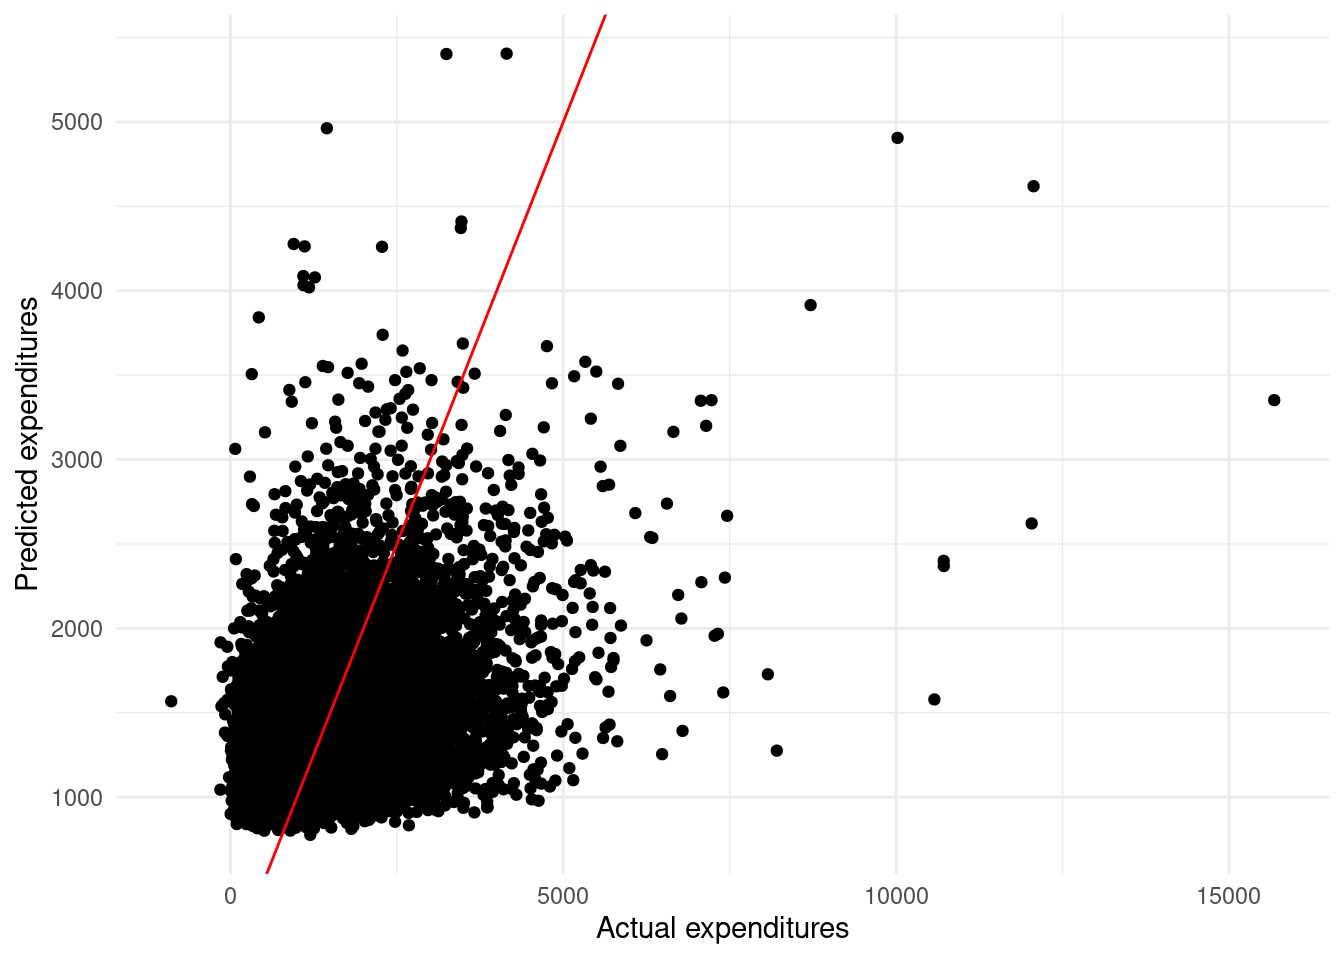
\includegraphics{bookdown_files/figure-latex/model-lin-sol-3-p1-1.pdf}
\caption{\label{fig:model-lin-sol-3-p1}Actual and predicted electricity expenditures}
\end{figure}

\begin{Shaded}
\begin{Highlighting}[]
\NormalTok{temps\_sqft\_exp\_fit }\SpecialCharTok{\%\textgreater{}\%}
  \FunctionTok{ggplot}\NormalTok{(}\FunctionTok{aes}\NormalTok{(}\AttributeTok{x =}\NormalTok{ .fitted, }\AttributeTok{y =}\NormalTok{ .resid)) }\SpecialCharTok{+}
  \FunctionTok{geom\_point}\NormalTok{() }\SpecialCharTok{+}
  \FunctionTok{geom\_hline}\NormalTok{(}\AttributeTok{yintercept =} \DecValTok{0}\NormalTok{, }\AttributeTok{color =} \StringTok{"red"}\NormalTok{) }\SpecialCharTok{+}
  \FunctionTok{xlab}\NormalTok{(}\StringTok{"Predicted expenditure"}\NormalTok{) }\SpecialCharTok{+}
  \FunctionTok{ylab}\NormalTok{(}\StringTok{"Residual value of expenditure"}\NormalTok{) }\SpecialCharTok{+}
  \FunctionTok{theme\_minimal}\NormalTok{()}
\end{Highlighting}
\end{Shaded}

\begin{figure}
\centering
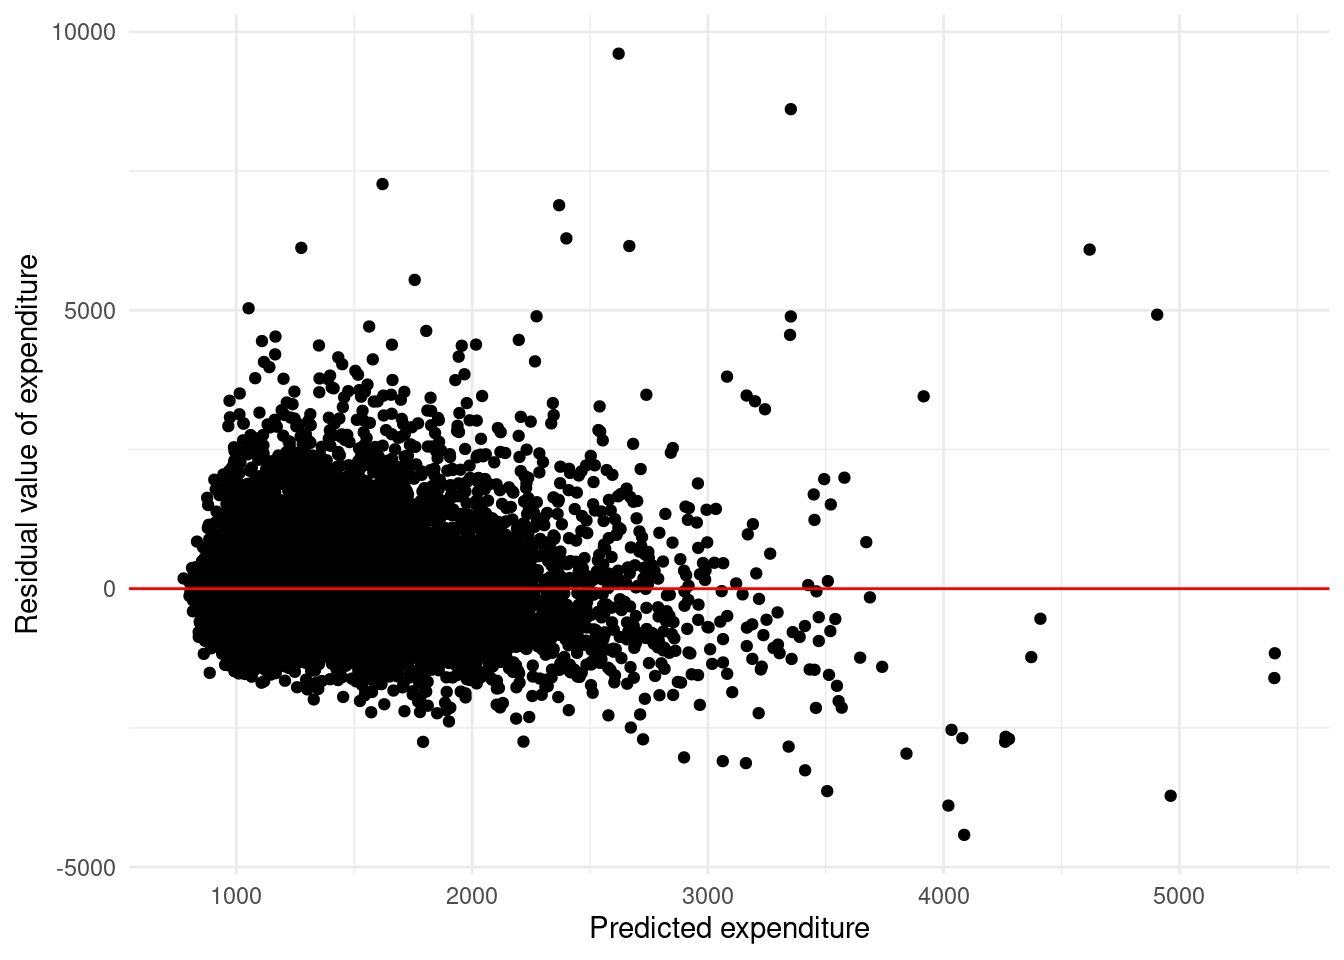
\includegraphics{bookdown_files/figure-latex/model-lin-sol-3-p2-1.pdf}
\caption{\label{fig:model-lin-sol-3-p2}Residual plot of electric cost model with covariates TOTSQFT\_EN, CDD65, and HDD65}
\end{figure}

\begin{enumerate}
\def\labelenumi{\arabic{enumi}.}
\setcounter{enumi}{3}
\tightlist
\item
  Early voting expanded in 2020\footnote{\url{https://www.npr.org/2020/10/26/927803214/62-million-and-counting-americans-are-breaking-early-voting-records}}. Using the ANES data, build a logistic model predicting early voting in 2020 (\texttt{EarlyVote2020}) using age (\texttt{Age}), education (\texttt{Education}), and party identification (\texttt{PartyID}). Include two-way interactions.
\end{enumerate}

\begin{Shaded}
\begin{Highlighting}[]
\NormalTok{earlyvote\_mod }\OtherTok{\textless{}{-}}\NormalTok{ anes\_des }\SpecialCharTok{\%\textgreater{}\%}
  \FunctionTok{filter}\NormalTok{(}\SpecialCharTok{!}\FunctionTok{is.na}\NormalTok{(EarlyVote2020)) }\SpecialCharTok{\%\textgreater{}\%}
  \FunctionTok{svyglm}\NormalTok{(}
    \AttributeTok{design =}\NormalTok{ .,}
    \AttributeTok{formula =}\NormalTok{ EarlyVote2020 }\SpecialCharTok{\textasciitilde{}}\NormalTok{ (Age }\SpecialCharTok{+}\NormalTok{ Education }\SpecialCharTok{+}\NormalTok{ PartyID)}\SpecialCharTok{\^{}}\DecValTok{2}\NormalTok{,}
    \AttributeTok{family =}\NormalTok{ quasibinomial}
\NormalTok{  )}

\FunctionTok{tidy}\NormalTok{(earlyvote\_mod) }\SpecialCharTok{\%\textgreater{}\%} \FunctionTok{arrange}\NormalTok{(p.value)}
\end{Highlighting}
\end{Shaded}

\begin{verbatim}
## # A tibble: 46 x 5
##    term                             estimate std.error statistic p.value
##    <chr>                               <dbl>     <dbl>     <dbl>   <dbl>
##  1 EducationPost HS:PartyIDNot ver~     16.2      1.69      9.54  0.0108
##  2 EducationGraduate:PartyIDNot ve~     15.4      1.72      8.95  0.0123
##  3 EducationBachelor's:PartyIDNot ~     15.8      1.93      8.18  0.0146
##  4 EducationGraduate:PartyIDIndepe~    -14.2      1.75     -8.12  0.0148
##  5 PartyIDIndependent-republican       -19.5      2.42     -8.09  0.0149
##  6 EducationHigh school:PartyIDNot~     15.9      2.02      7.88  0.0157
##  7 EducationBachelor's:PartyIDInde~     17.7      2.32      7.64  0.0167
##  8 EducationGraduate:PartyIDIndepe~     16.5      2.33      7.10  0.0193
##  9 EducationHigh school:PartyIDInd~     15.5      2.56      6.05  0.0262
## 10 EducationGraduate:PartyIDIndepe~    -14.8      2.47     -5.99  0.0268
## # i 36 more rows
\end{verbatim}

\begin{enumerate}
\def\labelenumi{\arabic{enumi}.}
\setcounter{enumi}{4}
\tightlist
\item
  Continuing from Exercise 4, predict the probability of early voting for two people. Both are 28 years old and have a graduate degree, but one person is a strong Democrat, and the other is a strong Republican.
\end{enumerate}

\begin{Shaded}
\begin{Highlighting}[]
\NormalTok{add\_vote\_dat }\OtherTok{\textless{}{-}}\NormalTok{ anes\_2020 }\SpecialCharTok{\%\textgreater{}\%}
  \FunctionTok{select}\NormalTok{(EarlyVote2020, Age, Education, PartyID) }\SpecialCharTok{\%\textgreater{}\%}
  \FunctionTok{rbind}\NormalTok{(}\FunctionTok{tibble}\NormalTok{(}
    \AttributeTok{EarlyVote2020 =} \ConstantTok{NA}\NormalTok{,}
    \AttributeTok{Age =} \DecValTok{28}\NormalTok{,}
    \AttributeTok{Education =} \StringTok{"Graduate"}\NormalTok{,}
    \AttributeTok{PartyID =} \FunctionTok{c}\NormalTok{(}\StringTok{"Strong democrat"}\NormalTok{, }\StringTok{"Strong republican"}\NormalTok{)}
\NormalTok{  )) }\SpecialCharTok{\%\textgreater{}\%}
  \FunctionTok{tail}\NormalTok{(}\DecValTok{2}\NormalTok{)}

\NormalTok{log\_ex\_2\_out }\OtherTok{\textless{}{-}}\NormalTok{ earlyvote\_mod }\SpecialCharTok{\%\textgreater{}\%}
  \FunctionTok{augment}\NormalTok{(}\AttributeTok{newdata =}\NormalTok{ add\_vote\_dat, }\AttributeTok{type.predict =} \StringTok{"response"}\NormalTok{) }\SpecialCharTok{\%\textgreater{}\%}
  \FunctionTok{mutate}\NormalTok{(}
    \AttributeTok{.se.fit =} \FunctionTok{sqrt}\NormalTok{(}\FunctionTok{attr}\NormalTok{(.fitted, }\StringTok{"var"}\NormalTok{)),}
    \CommentTok{\# extract the variance of the fitted value}
    \AttributeTok{.fitted =} \FunctionTok{as.numeric}\NormalTok{(.fitted)}
\NormalTok{  )}
\end{Highlighting}
\end{Shaded}

\hypertarget{part-reporting}{%
\part{Reporting}\label{part-reporting}}

\hypertarget{c08-communicating-results}{%
\chapter{Communicating results}\label{c08-communicating-results}}

\begin{prereqbox}{Prerequisites}

For this chapter, load the following packages:

\begin{Shaded}
\begin{Highlighting}[]
\FunctionTok{library}\NormalTok{(tidyverse)}
\FunctionTok{library}\NormalTok{(survey)}
\FunctionTok{library}\NormalTok{(srvyr)}
\FunctionTok{library}\NormalTok{(srvyrexploR)}
\FunctionTok{library}\NormalTok{(gt)}
\FunctionTok{library}\NormalTok{(gtsummary)}
\end{Highlighting}
\end{Shaded}

We will be using data from ANES as described in Chapter \ref{c04-getting-started}. As a reminder, here is the code to create the design objects for each to use throughout this chapter. For ANES, we need to adjust the weight so it sums to the population instead of the sample (see the ANES documentation and Chapter \ref{c04-getting-started} for more information).

\begin{Shaded}
\begin{Highlighting}[]
\NormalTok{targetpop }\OtherTok{\textless{}{-}} \DecValTok{231592693}
\FunctionTok{data}\NormalTok{(anes\_2020)}

\NormalTok{anes\_adjwgt }\OtherTok{\textless{}{-}}\NormalTok{ anes\_2020 }\SpecialCharTok{\%\textgreater{}\%}
  \FunctionTok{mutate}\NormalTok{(}\AttributeTok{Weight =}\NormalTok{ Weight }\SpecialCharTok{/} \FunctionTok{sum}\NormalTok{(Weight) }\SpecialCharTok{*}\NormalTok{ targetpop)}

\NormalTok{anes\_des }\OtherTok{\textless{}{-}}\NormalTok{ anes\_adjwgt }\SpecialCharTok{\%\textgreater{}\%}
  \FunctionTok{as\_survey\_design}\NormalTok{(}
    \AttributeTok{weights =}\NormalTok{ Weight,}
    \AttributeTok{strata =}\NormalTok{ Stratum,}
    \AttributeTok{ids =}\NormalTok{ VarUnit,}
    \AttributeTok{nest =} \ConstantTok{TRUE}
\NormalTok{  )}
\end{Highlighting}
\end{Shaded}

\end{prereqbox}

\hypertarget{introduction-6}{%
\section{Introduction}\label{introduction-6}}

After finishing the analysis and modeling, we proceed to the important task of communicating the survey results. Our audience may range from seasoned researchers familiar with our survey data to newcomers encountering the information for the first time. We should aim to explain the methodology and analysis while presenting findings in an accessible way, and it is our responsibility to report information with care.

Before beginning any dissemination of results, consider questions such as:

\begin{itemize}
\tightlist
\item
  How will we present results? Examples include a website, print, or other media. Based on the media type, we might limit or enhance the use of graphical representation.
\item
  What is the audience's familiarity with the study and/or data? Audiences can range from the general public to data experts. If we anticipate limited knowledge about the study, we should provide detailed descriptions (we discuss recommendations later in the chapter).
\item
  What are we trying to communicate? It could be summary statistics, trends, patterns, or other insights. Tables might suit summary statistics, while plots are better at conveying trends and patterns.
\item
  Is the audience accustomed to interpreting plots? If not, include explanatory text to guide them on how to interpret the plots effectively.
\item
  What is the audience's statistical knowledge? If the audience does not have a strong statistics background, provide text on standard errors, confidence intervals, and other estimate types to enhance understanding.
\end{itemize}

\hypertarget{describing-results-through-text}{%
\section{Describing results through text}\label{describing-results-through-text}}

As analysts, our emphasis is often on the data, and communicating results can sometimes be overlooked. First, we need to identify the appropriate information to share with our audience. Chapters \ref{c02-overview-surveys} and \ref{c03-understanding-survey-data-documentation} provide insights into factors we need to consider during analysis, and they remain relevant when presenting results to others.

\hypertarget{methodology-1}{%
\subsection{Methodology}\label{methodology-1}}

If we are using existing data, methodologically-sound surveys will provide documentation about how the survey was fielded, the questionnaires, and other necessary information for analyses. For example, the survey's methodology reports should include the population of interest, sampling procedures, response rates, questionnaire documentation, weighting, and a general overview of disclosure statements. Many American organizations follow the American Association for Public Opinion Research's (AAPOR) \href{https://aapor.org/standards-and-ethics/transparency-initiative}{Transparency Initiative}. The AAPOR Transparency Initiative requires organizations to include specific details in their methodology, making it clear how we can and should analyze the results. Being transparent about these methods is vital for the scientific rigor of the field.

The details provided in Chapter \ref{c02-overview-surveys} about the survey process should be shared with the audience when presenting the results. When using publicly-available data, like the examples in this book, we can often link to the methodology report in our final output. We should also provide high-level information for the audience to quickly grasp the context around the findings. For example, we can mention when and where the study was conducted, the population's age range, or other contextual details. This information helps the audience understand how generalizable the results are.

Providing this material is especially important when there's no methodology report available for the analyzed data. For example, if a researcher conducted a new survey for a specific purpose, we should document and present all the pertinent information during the analysis and reporting process. Adhering to the AAPOR Transparency Initiative guidelines is a reliable method to guarantee that all essential information is communicated to the audience.

\hypertarget{analysis}{%
\subsection{Analysis}\label{analysis}}

Along with the survey methodology and weight calculations, we should also share our approach to preparing, cleaning, and analyzing the data. For example, in Chapter \ref{c06-statistical-testing}, we compared education distributions from the ANES survey to the American Community Survey (ACS). To make the comparison, we had to collapse education categories provided in the ANES data to match the ACS. The process for this particular example may seem straightforward (like combining Bachelor's and Graduate Degrees into a single category), but there are multiple ways to deal with the data. Our choice is just one of many. We should document both the original ANES question and response options and the steps we took to match it with ACS data. This transparency helps clarify our analysis to our audience.

Missing data is another instance where we want to be unambigious and upfront with our audience. In this book, numerous examples and exercises remove missing data, as this is often the easiest way to handle them. However, there are circumstances where missing data holds substantive importance, and excluding them could introduce bias (see Chapter \ref{c11-missing-data}). Being transparent about our handling of missing data is important to maintaining the integrity of our analysis and ensuring a comprehensive understanding of the results.

\hypertarget{results}{%
\subsection{Results}\label{results}}

While tables and graphs are commonly used to communicate results, there are instances where text can be more effective in sharing information. Narrative details, such as context around point estimates or model coefficients, can go a long way in improving our communication. We have several strategies to effectively convey the significance of the data to the audience through text.

First, we can highlight important data points in a sentence using plain language. For example, if we were looking at election polling data conducted before an election, we could say something like:

\begin{quote}
As of {[}DATE{]}, an estimated XX\% of registered U.S. voters say they will vote for {[}CANDIDATE NAME{]} for president in the {[}YEAR{]} general election.
\end{quote}

This sentence provides key pieces of information in a straightforward way:

\begin{enumerate}
\def\labelenumi{\arabic{enumi}.}
\tightlist
\item
  \textbf{{[}DATE{]}}: Given that polling data is time-specific, providing the date of reference lets the audience know when this data was valid.
\item
  \textbf{Registered U.S. voters}: This tells the audience who we surveyed, letting them know the target population.
\item
  \textbf{XX\%}: This part provides the estimated percentage of people voting for a specific candidate for a specific office.
\item
  \textbf{{[}YEAR{]} general election}: As with the bullet above, adding this gives more context about the election type and year. The estimate would take on a different meaning if we changed it to a \emph{primary} election instead of a \emph{general} election.
\end{enumerate}

We also included the word ``estimated.'' When presenting aggregate survey results, we have errors around each estimate. We want to convey this uncertainty rather than talk in absolutes. Words like ``estimated,'' ``on average,'' or ``around'' can help communicate this uncertainty to the audience. Instead of saying `XX\%,' we can also say `XX\% (+/- Y\%)' to show the margin of error. Confidence intervals can also be incorporated into the text to assist readers.

Second, providing context and discussing the \emph{meaning} behind a point estimate can help the audience glean some insight into why the data is important. For example, when comparing two values, it can be helpful to highlight if there are statistically significant differences and explain the impact and relevance of this information. This is where we, as analysts, should to do our best to be mindful of biases and present the facts logically.

Keep in mind how we discuss these findings can greatly influence how the audience interprets them. If we include speculation, using phrases like ``the authors speculate'' or ``these findings may indicate'' relays the uncertainty around the notion while still lending a plausible solution. Additionally, we can present alternative viewpoints or competing discussion points to explain the uncertainty in the results.

\hypertarget{visualizing-data}{%
\section{Visualizing data}\label{visualizing-data}}

Although discussing key findings in the text is important, presenting large amounts of data is often more digestible for the audience in tables or visualizations. Effectively combining text, tables, and graphs can be powerful in communicating results. This section provides examples of using the \{gt\}, \{gtsummary\}, and \{ggplot2\} packages to enhance the dissemination of results.

\hypertarget{tables}{%
\subsection{Tables}\label{tables}}

Tables are a great way to provide a large amount of data when individual data points need to be examined. However, it is important to present tables in a reader-friendly format. Numbers should align, rows and columns should be easy to follow, and the table size should not compromise readability. Using key visualization techniques, we can create tables that are informative and nice to look at. Many packages create easy-to-read tables (e.g., \{kable\} + \{kableExtra\}, \{gt\}, \{gtsummary\}, \{DT\}, \{formattable\}, \{flextable\}, \{reactable\}). While we will focus on \{gt\} here, we encourage learning about others as they may have additional helpful features. We appreciate the flexibility, ability to use pipes (e.g., \texttt{\%\textgreater{}\%}), and numerous extensions of the \{gt\} package. Please note, at this time, \{gtsummary\} needs additional features to be widely used for survey analysis, particularly due to its lack of ability to work with replicate designs. We provide one example using \{gtsummary\} and hope it evolves into a more comprehensive tool over time.

\hypertarget{results-gt}{%
\subsubsection{Transitioning \{srvyr\} output to a \{gt\} table}\label{results-gt}}

Let's start by using some of the data we calculated earlier in this book. In Chapter \ref{c06-statistical-testing}, we looked at data on trust in government with the proportions calculated below:

\begin{Shaded}
\begin{Highlighting}[]
\NormalTok{trust\_gov }\OtherTok{\textless{}{-}}\NormalTok{ anes\_des }\SpecialCharTok{\%\textgreater{}\%}
  \FunctionTok{drop\_na}\NormalTok{(TrustGovernment) }\SpecialCharTok{\%\textgreater{}\%}
  \FunctionTok{group\_by}\NormalTok{(TrustGovernment) }\SpecialCharTok{\%\textgreater{}\%}
  \FunctionTok{summarize}\NormalTok{(}\AttributeTok{trust\_gov\_p =} \FunctionTok{survey\_prop}\NormalTok{())}

\NormalTok{trust\_gov}
\end{Highlighting}
\end{Shaded}

\begin{verbatim}
## # A tibble: 5 x 3
##   TrustGovernment     trust_gov_p trust_gov_p_se
##   <fct>                     <dbl>          <dbl>
## 1 Always                   0.0155        0.00204
## 2 Most of the time         0.132         0.00553
## 3 About half the time      0.309         0.00829
## 4 Some of the time         0.434         0.00855
## 5 Never                    0.110         0.00566
\end{verbatim}

The default output generated by R may work for initial viewing inside our IDE or when creating basic output in an R Markdown or Quarto document. However, when presenting these results in other publications, such as the print version of this book or with other formal dissemination modes, modifying the display can improve our reader's experience.

Looking at the output from \texttt{trust\_gov}, a couple of improvements are obvious: (1) switching to percentages instead of proportions and (2) using the variable names as column headers. The \{gt\} package is a good tool for implementing better labeling and creating publishable tables. Let's walk through some code as we make a few changes to improve the table's usefulness.

First, we initiate the table with the \texttt{gt()} function. Next, we use the argument \texttt{rowname\_col()} to designate the \texttt{TrustGovernment} column as the labels for each row (called the table ``stub''). We apply the \texttt{cols\_label()} function to create informative column labels instead of variable names, and then the \texttt{tab\_spanner()} function to add a label across multiple columns. In this case, we label all columns except the stub with ``Trust in Government, 2020''. We then format the proportions into percentages with the \texttt{fmt\_percent()} function and reduce the number of decimals shown with \texttt{decimals\ =\ 1}. Finally, the \texttt{tab\_caption()} function adds a table title for HTML version of the book. We can use the caption for cross-referencing in R Markdown, Quarto, and bookdown, as well as adding it to the list of tables in the book.

\begin{Shaded}
\begin{Highlighting}[]
\NormalTok{trust\_gov\_gt }\OtherTok{\textless{}{-}}\NormalTok{ trust\_gov }\SpecialCharTok{\%\textgreater{}\%}
  \FunctionTok{gt}\NormalTok{(}\AttributeTok{rowname\_col =} \StringTok{"TrustGovernment"}\NormalTok{) }\SpecialCharTok{\%\textgreater{}\%}
  \FunctionTok{cols\_label}\NormalTok{(}
    \AttributeTok{trust\_gov\_p =} \StringTok{"\%"}\NormalTok{,}
    \AttributeTok{trust\_gov\_p\_se =} \StringTok{"s.e. (\%)"}
\NormalTok{  ) }\SpecialCharTok{\%\textgreater{}\%}
  \FunctionTok{tab\_spanner}\NormalTok{(}
    \AttributeTok{label =} \StringTok{"Trust in Government, 2020"}\NormalTok{,}
    \AttributeTok{columns =} \FunctionTok{c}\NormalTok{(trust\_gov\_p, trust\_gov\_p\_se)}
\NormalTok{  ) }\SpecialCharTok{\%\textgreater{}\%}
  \FunctionTok{fmt\_percent}\NormalTok{(}\AttributeTok{decimals =} \DecValTok{1}\NormalTok{)}
\end{Highlighting}
\end{Shaded}

\begin{Shaded}
\begin{Highlighting}[]
\NormalTok{trust\_gov\_gt }\SpecialCharTok{\%\textgreater{}\%}
  \FunctionTok{tab\_caption}\NormalTok{(}\StringTok{"Example of gt table with trust in government estimate"}\NormalTok{)}
\end{Highlighting}
\end{Shaded}



\begin{longtable}{l|rr}
\caption{\label{tab:results-table-gt1-tab}Example of gt table with trust in government estimate}\\
\toprule
\multicolumn{1}{l}{} & \multicolumn{2}{c}{Trust in Government, 2020} \\ 
\cmidrule(lr){2-3}
\multicolumn{1}{l}{} & \% & s.e. (\%) \\ 
\midrule
Always & $1.6\%$ & $0.2\%$ \\ 
Most of the time & $13.2\%$ & $0.6\%$ \\ 
About half the time & $30.9\%$ & $0.8\%$ \\ 
Some of the time & $43.4\%$ & $0.9\%$ \\ 
Never & $11.0\%$ & $0.6\%$ \\ 
\bottomrule
\end{longtable}

We can add a few more enhancements, such as a title, a data source note, and a footnote with the question information, using the functions \texttt{tab\_header()}, \texttt{tab\_source\_note()}, and \texttt{tab\_footnote()}. If having the percentage sign in both the header and the cells seems redundant, we can opt for \texttt{fmt\_number()} instead of \texttt{fmt\_percent()} and scale the number by 100 with \texttt{scale\_by\ =\ 100}.

\begin{Shaded}
\begin{Highlighting}[]
\NormalTok{trust\_gov\_gt2 }\OtherTok{\textless{}{-}}\NormalTok{ trust\_gov\_gt }\SpecialCharTok{\%\textgreater{}\%}
  \FunctionTok{tab\_header}\NormalTok{(}\StringTok{"American voter\textquotesingle{}s trust}
\StringTok{             in the federal government, 2020"}\NormalTok{) }\SpecialCharTok{\%\textgreater{}\%}
  \FunctionTok{tab\_source\_note}\NormalTok{(}\StringTok{"American National Election Studies, 2020"}\NormalTok{) }\SpecialCharTok{\%\textgreater{}\%}
  \FunctionTok{tab\_footnote}\NormalTok{(}
    \StringTok{"Question text: How often can you trust the federal government}
\StringTok{    in Washington to do what is right?"}
\NormalTok{  ) }\SpecialCharTok{\%\textgreater{}\%}
  \FunctionTok{fmt\_number}\NormalTok{(}
    \AttributeTok{scale\_by =} \DecValTok{100}\NormalTok{,}
    \AttributeTok{decimals =} \DecValTok{1}
\NormalTok{  )}
\end{Highlighting}
\end{Shaded}

\begin{Shaded}
\begin{Highlighting}[]
\NormalTok{trust\_gov\_gt2}
\end{Highlighting}
\end{Shaded}



\setlength{\LTpost}{0mm}
\begin{longtable}{l|rr}
\caption{\label{tab:results-table-gt2-tab}Example of gt table with trust in government estimates and additional context}\\
\caption*{
{\large American voter's trust
             in the federal government, 2020}
} \\ 
\toprule
\multicolumn{1}{l}{} & \multicolumn{2}{c}{Trust in Government, 2020} \\ 
\cmidrule(lr){2-3}
\multicolumn{1}{l}{} & \% & s.e. (\%) \\ 
\midrule
Always & $1.6$ & $0.2$ \\ 
Most of the time & $13.2$ & $0.6$ \\ 
About half the time & $30.9$ & $0.8$ \\ 
Some of the time & $43.4$ & $0.9$ \\ 
Never & $11.0$ & $0.6$ \\ 
\bottomrule
\end{longtable}
\begin{minipage}{\linewidth}
Question text: How often can you trust the federal government
    in Washington to do what is right?\\
American National Election Studies, 2020\\
\end{minipage}

\hypertarget{expanding-tables-using-gtsummary}{%
\subsubsection*{Expanding tables using \{gtsummary\}}\label{expanding-tables-using-gtsummary}}


The \{gtsummary\} package simultaneously summarizes data and creates publication-ready tables. Initially designed for clinical trial data, it has been extended to include survey analysis in certain capacities. At this time, it is only compatible with survey objects using Taylor's Series Linearization and not replicate methods. While it offers a restricted set of summary statistics, the following are available for categorical variables:

\begin{itemize}
\tightlist
\item
  \texttt{\{n\}} frequency
\item
  \texttt{\{N\}} denominator, or cohort size
\item
  \texttt{\{p\}} percentage
\item
  \texttt{\{p.std.error\}} standard error of the sample proportion
\item
  \texttt{\{deff\}} design effect of the sample proportion
\item
  \texttt{\{n\_unweighted\}} unweighted frequency
\item
  \texttt{\{N\_unweighted\}} unweighted denominator
\item
  \texttt{\{p\_unweighted\}} unweighted formatted percentage
\end{itemize}

The following summary statistics are available for continuous variables:

\begin{itemize}
\tightlist
\item
  \texttt{\{median\}} median
\item
  \texttt{\{mean\}} mean
\item
  \texttt{\{mean.std.error\}} standard error of the sample mean
\item
  \texttt{\{deff\}} design effect of the sample mean
\item
  \texttt{\{sd\}} standard deviation
\item
  \texttt{\{var\}} variance
\item
  \texttt{\{min\}} minimum
\item
  \texttt{\{max\}} maximum
\item
  \texttt{\{p\#\#\}} any integer percentile, where \texttt{\#\#} is an integer from 0 to 100
\item
  \texttt{\{sum\}} sum
\end{itemize}

In the following example, we will build a table using \{gtsummary\}, similar to the table in the \{gt\} example. The main function we use is \texttt{tbl\_svysummary()}. In this function, we include the variables we want to analyze in the \texttt{include} argument and define the statistics we want to display in the \texttt{statistic} argument. To specify the statistics, we apply the syntax from the \{glue\} package, where we enclose the variables we want to insert within curly brackets. We must specify the desired statistics using the names listed above. For example, to specify that we want the proportion followed by the standard error of the proportion in parentheses, we use \texttt{\{p\}\ (\{p.std.error\})}.

\begin{Shaded}
\begin{Highlighting}[]
\NormalTok{anes\_des\_gtsum }\OtherTok{\textless{}{-}}\NormalTok{ anes\_des }\SpecialCharTok{\%\textgreater{}\%}
  \FunctionTok{tbl\_svysummary}\NormalTok{(}
    \AttributeTok{include =}\NormalTok{ TrustGovernment,}
    \AttributeTok{statistic =} \FunctionTok{list}\NormalTok{(}\FunctionTok{all\_categorical}\NormalTok{() }\SpecialCharTok{\textasciitilde{}} \StringTok{"\{p\} (\{p.std.error\})"}\NormalTok{)}
\NormalTok{  )}
\end{Highlighting}
\end{Shaded}

\begin{Shaded}
\begin{Highlighting}[]
\NormalTok{anes\_des\_gtsum}
\end{Highlighting}
\end{Shaded}



\setlength{\LTpost}{0mm}
\begin{longtable}{lc}
\caption{\label{tab:results-gts-ex-1-tab}Example of gtsummary table with trust in government estimates}\\
\toprule
\textbf{Characteristic} & \textbf{N = 231,034,125}\textsuperscript{\textit{1}} \\ 
\midrule
PRE: How often trust government in Washington to do what is right [revised] &  \\ 
    Always & 1.6 (0.00) \\ 
    Most of the time & 13 (0.01) \\ 
    About half the time & 31 (0.01) \\ 
    Some of the time & 43 (0.01) \\ 
    Never & 11 (0.01) \\ 
    Unknown & 673,773 \\ 
\bottomrule
\end{longtable}
\begin{minipage}{\linewidth}
\textsuperscript{\textit{1}}\% (SE(\%))\\
\end{minipage}

The default table includes the weighted number of missing (or Unknown) records. The standard error is reported as a proportion, while the proportion is styled as a percentage. In the next step, we remove the Unknown category by setting the missing argument to ``no'' and format the standard error as a percentage using the \texttt{digits} argument. To improve the table for publication, we provide a more polished label for the ``TrustGovernment'' variable using the \texttt{label} argument.

\begin{Shaded}
\begin{Highlighting}[]
\NormalTok{anes\_des\_gtsum2 }\OtherTok{\textless{}{-}}\NormalTok{ anes\_des }\SpecialCharTok{\%\textgreater{}\%}
  \FunctionTok{tbl\_svysummary}\NormalTok{(}
    \AttributeTok{include =}\NormalTok{ TrustGovernment,}
    \AttributeTok{statistic =} \FunctionTok{list}\NormalTok{(}\FunctionTok{all\_categorical}\NormalTok{() }\SpecialCharTok{\textasciitilde{}} \StringTok{"\{p\} (\{p.std.error\})"}\NormalTok{),}
    \AttributeTok{missing =} \StringTok{"no"}\NormalTok{,}
    \AttributeTok{digits =} \FunctionTok{list}\NormalTok{(TrustGovernment }\SpecialCharTok{\textasciitilde{}}\NormalTok{ style\_percent),}
    \AttributeTok{label =} \FunctionTok{list}\NormalTok{(TrustGovernment }\SpecialCharTok{\textasciitilde{}} \StringTok{"Trust in Government, 2020"}\NormalTok{)}
\NormalTok{  )}
\end{Highlighting}
\end{Shaded}

\begin{Shaded}
\begin{Highlighting}[]
\NormalTok{anes\_des\_gtsum2}
\end{Highlighting}
\end{Shaded}



\setlength{\LTpost}{0mm}
\begin{longtable}{lc}
\caption{\label{tab:results-gts-ex-2-tab}Example of gtsummary table with trust in government estimates with labeling and digits options}\\
\toprule
\textbf{Characteristic} & \textbf{N = 231,034,125}\textsuperscript{\textit{1}} \\ 
\midrule
Trust in Government, 2020 &  \\ 
    Always & 1.6 (0.2) \\ 
    Most of the time & 13 (0.6) \\ 
    About half the time & 31 (0.8) \\ 
    Some of the time & 43 (0.9) \\ 
    Never & 11 (0.6) \\ 
\bottomrule
\end{longtable}
\begin{minipage}{\linewidth}
\textsuperscript{\textit{1}}\% (SE(\%))\\
\end{minipage}

To exclude the term ``Characteristic'' and the estimated population size, we can modify the header using the\texttt{modify\_header()} function to update the \texttt{label}. Further adjustments can be made based on personal preferences, organizational guidelines, or other style guides. If we prefer having the standard error in the header, similar to the \{gt\} table, instead of in the footnote (the \{gtsummary\} default), we can make these changes by specifying \texttt{stat\_0} in the \texttt{modify\_header()} function. Additionally, using \texttt{modify\_footnote()} with \texttt{update\ =\ everything()\ \textasciitilde{}\ NA} removes the standard error from the footnote. After transforming the object into a gt table using \texttt{as\_gt()}, we can add footnotes and a title using the same methods explained in Section \ref{results-gt}.

\begin{Shaded}
\begin{Highlighting}[]
\NormalTok{anes\_des\_gtsum3 }\OtherTok{\textless{}{-}}\NormalTok{ anes\_des }\SpecialCharTok{\%\textgreater{}\%}
  \FunctionTok{tbl\_svysummary}\NormalTok{(}
    \AttributeTok{include =}\NormalTok{ TrustGovernment,}
    \AttributeTok{statistic =} \FunctionTok{list}\NormalTok{(}\FunctionTok{all\_categorical}\NormalTok{() }\SpecialCharTok{\textasciitilde{}} \StringTok{"\{p\} (\{p.std.error\})"}\NormalTok{),}
    \AttributeTok{missing =} \StringTok{"no"}\NormalTok{,}
    \AttributeTok{digits =} \FunctionTok{list}\NormalTok{(TrustGovernment }\SpecialCharTok{\textasciitilde{}}\NormalTok{ style\_percent),}
    \AttributeTok{label =} \FunctionTok{list}\NormalTok{(TrustGovernment }\SpecialCharTok{\textasciitilde{}} \StringTok{"Trust in Government, 2020"}\NormalTok{)}
\NormalTok{  ) }\SpecialCharTok{\%\textgreater{}\%}
  \FunctionTok{modify\_footnote}\NormalTok{(}\AttributeTok{update =} \FunctionTok{everything}\NormalTok{() }\SpecialCharTok{\textasciitilde{}} \ConstantTok{NA}\NormalTok{) }\SpecialCharTok{\%\textgreater{}\%}
  \FunctionTok{modify\_header}\NormalTok{(}
    \AttributeTok{label =} \StringTok{" "}\NormalTok{,}
    \AttributeTok{stat\_0 =} \StringTok{"\% (s.e.)"}
\NormalTok{  ) }\SpecialCharTok{\%\textgreater{}\%}
  \FunctionTok{as\_gt}\NormalTok{() }\SpecialCharTok{\%\textgreater{}\%}
  \FunctionTok{tab\_header}\NormalTok{(}\StringTok{"American voter\textquotesingle{}s trust}
\StringTok{             in the federal government, 2020"}\NormalTok{) }\SpecialCharTok{\%\textgreater{}\%}
  \FunctionTok{tab\_source\_note}\NormalTok{(}\StringTok{"American National Election Studies, 2020"}\NormalTok{) }\SpecialCharTok{\%\textgreater{}\%}
  \FunctionTok{tab\_footnote}\NormalTok{(}
    \StringTok{"Question text: How often can you trust}
\StringTok{    the federal government in Washington}
\StringTok{    to do what is right?"}
\NormalTok{  )}
\end{Highlighting}
\end{Shaded}

\begin{Shaded}
\begin{Highlighting}[]
\NormalTok{anes\_des\_gtsum3}
\end{Highlighting}
\end{Shaded}



\setlength{\LTpost}{0mm}
\begin{longtable}{lc}
\caption{\label{tab:results-gts-ex-3-tab}Example of gtsummary table with trust in government estimates with more labeling options and context}\\
\caption*{
{\large American voter's trust
             in the federal government, 2020}
} \\ 
\toprule
 & \% (s.e.) \\ 
\midrule
Trust in Government, 2020 &  \\ 
    Always & 1.6 (0.2) \\ 
    Most of the time & 13 (0.6) \\ 
    About half the time & 31 (0.8) \\ 
    Some of the time & 43 (0.9) \\ 
    Never & 11 (0.6) \\ 
\bottomrule
\end{longtable}
\begin{minipage}{\linewidth}
Question text: How often can you trust
    the federal government in Washington
    to do what is right?\\
American National Election Studies, 2020\\
\end{minipage}

We can also include continuous variables in the table. Below, we add a summary of the age variable by updating the \texttt{include}, \texttt{statistic}, and \texttt{digits} arguments.

\begin{Shaded}
\begin{Highlighting}[]
\NormalTok{anes\_des\_gtsum4 }\OtherTok{\textless{}{-}}\NormalTok{ anes\_des }\SpecialCharTok{\%\textgreater{}\%}
  \FunctionTok{tbl\_svysummary}\NormalTok{(}
    \AttributeTok{include =} \FunctionTok{c}\NormalTok{(TrustGovernment, Age),}
    \AttributeTok{statistic =} \FunctionTok{list}\NormalTok{(}
      \FunctionTok{all\_categorical}\NormalTok{() }\SpecialCharTok{\textasciitilde{}} \StringTok{"\{p\} (\{p.std.error\})"}\NormalTok{,}
      \FunctionTok{all\_continuous}\NormalTok{() }\SpecialCharTok{\textasciitilde{}} \StringTok{"\{mean\} (\{mean.std.error\})"}
\NormalTok{    ),}
    \AttributeTok{missing =} \StringTok{"no"}\NormalTok{,}
    \AttributeTok{digits =} \FunctionTok{list}\NormalTok{(TrustGovernment }\SpecialCharTok{\textasciitilde{}}\NormalTok{ style\_percent,}
\NormalTok{                  Age }\SpecialCharTok{\textasciitilde{}} \FunctionTok{c}\NormalTok{(}\DecValTok{1}\NormalTok{, }\DecValTok{2}\NormalTok{)),}
    \AttributeTok{label =} \FunctionTok{list}\NormalTok{(TrustGovernment }\SpecialCharTok{\textasciitilde{}} \StringTok{"Trust in Government, 2020"}\NormalTok{)}
\NormalTok{  ) }\SpecialCharTok{\%\textgreater{}\%}
  \FunctionTok{modify\_footnote}\NormalTok{(}\AttributeTok{update =} \FunctionTok{everything}\NormalTok{() }\SpecialCharTok{\textasciitilde{}} \ConstantTok{NA}\NormalTok{) }\SpecialCharTok{\%\textgreater{}\%}
  \FunctionTok{modify\_header}\NormalTok{(}\AttributeTok{label =} \StringTok{" "}\NormalTok{,}
                \AttributeTok{stat\_0 =} \StringTok{"\% (s.e.)"}\NormalTok{) }\SpecialCharTok{\%\textgreater{}\%}
  \FunctionTok{as\_gt}\NormalTok{() }\SpecialCharTok{\%\textgreater{}\%}
  \FunctionTok{tab\_header}\NormalTok{(}\StringTok{"American voter\textquotesingle{}s trust in the federal government, 2020"}\NormalTok{) }\SpecialCharTok{\%\textgreater{}\%}
  \FunctionTok{tab\_source\_note}\NormalTok{(}\StringTok{"American National Election Studies, 2020"}\NormalTok{) }\SpecialCharTok{\%\textgreater{}\%}
  \FunctionTok{tab\_footnote}\NormalTok{(}
    \StringTok{"Question text: How often can you trust the federal government}
\StringTok{    in Washington to do what is right?"}
\NormalTok{  ) }\SpecialCharTok{\%\textgreater{}\%}
  \FunctionTok{tab\_caption}\NormalTok{(}\StringTok{"Example of gtsummary table with trust in government}
\StringTok{              estimates and average age"}\NormalTok{)}
\end{Highlighting}
\end{Shaded}

\begin{Shaded}
\begin{Highlighting}[]
\NormalTok{anes\_des\_gtsum4}
\end{Highlighting}
\end{Shaded}



\setlength{\LTpost}{0mm}
\begin{longtable}{lc}
\caption{\label{tab:results-gts-ex-4-tab}Example of gtsummary table with trust in government estimates and average age}\\
\caption*{
{\large American voter's trust in the federal government, 2020}
} \\ 
\toprule
 & \% (s.e.) \\ 
\midrule
Trust in Government, 2020 &  \\ 
    Always & 1.6 (0.2) \\ 
    Most of the time & 13 (0.6) \\ 
    About half the time & 31 (0.8) \\ 
    Some of the time & 43 (0.9) \\ 
    Never & 11 (0.6) \\ 
PRE: SUMMARY: Respondent age & 47.3 (0.36) \\ 
\bottomrule
\end{longtable}
\begin{minipage}{\linewidth}
Question text: How often can you trust the federal government
    in Washington to do what is right?\\
American National Election Studies, 2020\\
\end{minipage}

With \{gtsummary\}, we can also calculate statistics by different groups. Let's modify the previous example to analyze data on whether a respondent voted for president in 2020. We update the \texttt{by} argument and refine the header.

\begin{Shaded}
\begin{Highlighting}[]
\NormalTok{anes\_des\_gtsum5 }\OtherTok{\textless{}{-}}\NormalTok{ anes\_des }\SpecialCharTok{\%\textgreater{}\%}
  \FunctionTok{drop\_na}\NormalTok{(VotedPres2020) }\SpecialCharTok{\%\textgreater{}\%}
  \FunctionTok{tbl\_svysummary}\NormalTok{(}
    \AttributeTok{include =}\NormalTok{ TrustGovernment,}
    \AttributeTok{statistic =} \FunctionTok{list}\NormalTok{(}\FunctionTok{all\_categorical}\NormalTok{() }\SpecialCharTok{\textasciitilde{}} \StringTok{"\{p\} (\{p.std.error\})"}\NormalTok{),}
    \AttributeTok{missing =} \StringTok{"no"}\NormalTok{,}
    \AttributeTok{digits =} \FunctionTok{list}\NormalTok{(TrustGovernment }\SpecialCharTok{\textasciitilde{}}\NormalTok{ style\_percent),}
    \AttributeTok{label =} \FunctionTok{list}\NormalTok{(TrustGovernment }\SpecialCharTok{\textasciitilde{}} \StringTok{"Trust in Government, 2020"}\NormalTok{),}
    \AttributeTok{by =}\NormalTok{ VotedPres2020}
\NormalTok{  ) }\SpecialCharTok{\%\textgreater{}\%}
  \FunctionTok{modify\_footnote}\NormalTok{(}\AttributeTok{update =} \FunctionTok{everything}\NormalTok{() }\SpecialCharTok{\textasciitilde{}} \ConstantTok{NA}\NormalTok{) }\SpecialCharTok{\%\textgreater{}\%}
  \FunctionTok{modify\_header}\NormalTok{(}
    \AttributeTok{label =} \StringTok{" "}\NormalTok{,}
    \AttributeTok{stat\_1 =} \StringTok{"Voted"}\NormalTok{,}
    \AttributeTok{stat\_2 =} \StringTok{"Didn\textquotesingle{}t vote"}
\NormalTok{  ) }\SpecialCharTok{\%\textgreater{}\%}
  \FunctionTok{as\_gt}\NormalTok{() }\SpecialCharTok{\%\textgreater{}\%}
  \FunctionTok{tab\_header}\NormalTok{(}
    \StringTok{"American voter\textquotesingle{}s trust}
\StringTok{             in the federal government by whether they voted}
\StringTok{             in the 2020 presidential election"}
\NormalTok{  ) }\SpecialCharTok{\%\textgreater{}\%}
  \FunctionTok{tab\_source\_note}\NormalTok{(}\StringTok{"American National Election Studies, 2020"}\NormalTok{) }\SpecialCharTok{\%\textgreater{}\%}
  \FunctionTok{tab\_footnote}\NormalTok{(}
    \StringTok{"Question text: How often can you trust the federal government}
\StringTok{               in Washington to do what is right?"}
\NormalTok{  )}
\end{Highlighting}
\end{Shaded}

\begin{Shaded}
\begin{Highlighting}[]
\NormalTok{anes\_des\_gtsum5}
\end{Highlighting}
\end{Shaded}



\setlength{\LTpost}{0mm}
\begin{longtable}{lcc}
\caption{\label{tab:results-gts-ex-5-tab}Example of gtsummary table with trust in government estimates by voting status}\\
\caption*{
{\large American voter's trust
             in the federal government by whether they voted
             in the 2020 presidential election}
} \\ 
\toprule
 & Voted & Didn't vote \\ 
\midrule
Trust in Government, 2020 &  &  \\ 
    Always & 1.1 (0.2) & 0.9 (0.9) \\ 
    Most of the time & 13 (0.6) & 19 (5.3) \\ 
    About half the time & 32 (0.8) & 30 (8.6) \\ 
    Some of the time & 45 (0.8) & 45 (8.2) \\ 
    Never & 9.1 (0.7) & 5.2 (2.2) \\ 
\bottomrule
\end{longtable}
\begin{minipage}{\linewidth}
Question text: How often can you trust the federal government
               in Washington to do what is right?\\
American National Election Studies, 2020\\
\end{minipage}

\hypertarget{charts-and-plots}{%
\subsection{Charts and plots}\label{charts-and-plots}}

Survey analysis can yield an abundance of printed summary statistics and models. Even with the most careful analysis, interpreting the results can be overwhelming. This is where charts and plots play a key role in our work. By transforming complex data into a visual representation, we can recognize patterns, relationships, and trends with greater ease.

R has numerous packages for creating compelling and insightful charts. In this section, we will focus on \{ggplot2\}, a member of the \{tidyverse\} collection of packages. Known for its power and flexibility, \{ggplot2\} is an invaluable tool for creating a wide range of data visualizations.

The \{ggplot2\} package follows the ``grammar of graphics,'' a framework that incrementally adds layers of chart components. This approach allows us to customize visual elements such as scales, colors, labels, and annotations to enhance the clarity of our results. After creating the survey design object, we can modify it to include additional outcomes and calculate estimates for our desired data points. Below, we create a binary variable \texttt{TrustGovernmentUsually}, which is \texttt{TRUE} when \texttt{TrustGovernment} is ``Always'' or ``Most of the time'' and \texttt{FALSE} otherwise. Then, we calculate the percentage of people who usually trust the government based on their vote in the 2020 presidential election (\texttt{VotedPres2020\_selection}). We remove the cases where people did not vote or did not indicate their choice.

\begin{Shaded}
\begin{Highlighting}[]
\NormalTok{anes\_des\_der }\OtherTok{\textless{}{-}}\NormalTok{ anes\_des }\SpecialCharTok{\%\textgreater{}\%}
  \FunctionTok{mutate}\NormalTok{(}\AttributeTok{TrustGovernmentUsually =} \FunctionTok{case\_when}\NormalTok{(}
    \FunctionTok{is.na}\NormalTok{(TrustGovernment) }\SpecialCharTok{\textasciitilde{}} \ConstantTok{NA}\NormalTok{,}
    \ConstantTok{TRUE} \SpecialCharTok{\textasciitilde{}}\NormalTok{ TrustGovernment }\SpecialCharTok{\%in\%} \FunctionTok{c}\NormalTok{(}\StringTok{"Always"}\NormalTok{, }\StringTok{"Most of the time"}\NormalTok{)}
\NormalTok{  )) }\SpecialCharTok{\%\textgreater{}\%}
  \FunctionTok{drop\_na}\NormalTok{(VotedPres2020\_selection) }\SpecialCharTok{\%\textgreater{}\%}
  \FunctionTok{group\_by}\NormalTok{(VotedPres2020\_selection) }\SpecialCharTok{\%\textgreater{}\%}
  \FunctionTok{summarize}\NormalTok{(}
    \AttributeTok{pct\_trust =} \FunctionTok{survey\_mean}\NormalTok{(}
\NormalTok{      TrustGovernmentUsually,}
      \AttributeTok{na.rm =} \ConstantTok{TRUE}\NormalTok{,}
      \AttributeTok{proportion =} \ConstantTok{TRUE}\NormalTok{,}
      \AttributeTok{vartype =} \StringTok{"ci"}
\NormalTok{    ),}
    \AttributeTok{.groups =} \StringTok{"drop"}
\NormalTok{  )}

\NormalTok{anes\_des\_der}
\end{Highlighting}
\end{Shaded}

\begin{verbatim}
## # A tibble: 3 x 4
##   VotedPres2020_selection pct_trust pct_trust_low pct_trust_upp
##   <fct>                       <dbl>         <dbl>         <dbl>
## 1 Biden                      0.123         0.109          0.140
## 2 Trump                      0.178         0.161          0.198
## 3 Other                      0.0681        0.0290         0.152
\end{verbatim}

Now, we can begin creating our chart with \{ggplot2\}. First, we set up our plot with \texttt{ggplot()}. Next, we define the data points to be displayed using aesthetics, or \texttt{aes}. Aesthetics represent the visual properties of the objects in the plot. In the example below, we map the \texttt{x} variable to \texttt{VotedPres2020\_selection} from the dataset and the \texttt{y} variable to \texttt{pct\_trust}. Finally, we specify the type of plot with \texttt{geom\_*()}, in this case, \texttt{geom\_bar()}. The resulting plot is displayed in Figure \ref{fig:results-plot1}.

\begin{Shaded}
\begin{Highlighting}[]
\NormalTok{p }\OtherTok{\textless{}{-}}\NormalTok{ anes\_des\_der }\SpecialCharTok{\%\textgreater{}\%}
  \FunctionTok{ggplot}\NormalTok{(}\FunctionTok{aes}\NormalTok{(}
    \AttributeTok{x =}\NormalTok{ VotedPres2020\_selection,}
    \AttributeTok{y =}\NormalTok{ pct\_trust}
\NormalTok{  )) }\SpecialCharTok{+}
  \FunctionTok{geom\_bar}\NormalTok{(}\AttributeTok{stat =} \StringTok{"identity"}\NormalTok{)}

\NormalTok{p}
\end{Highlighting}
\end{Shaded}

\begin{figure}
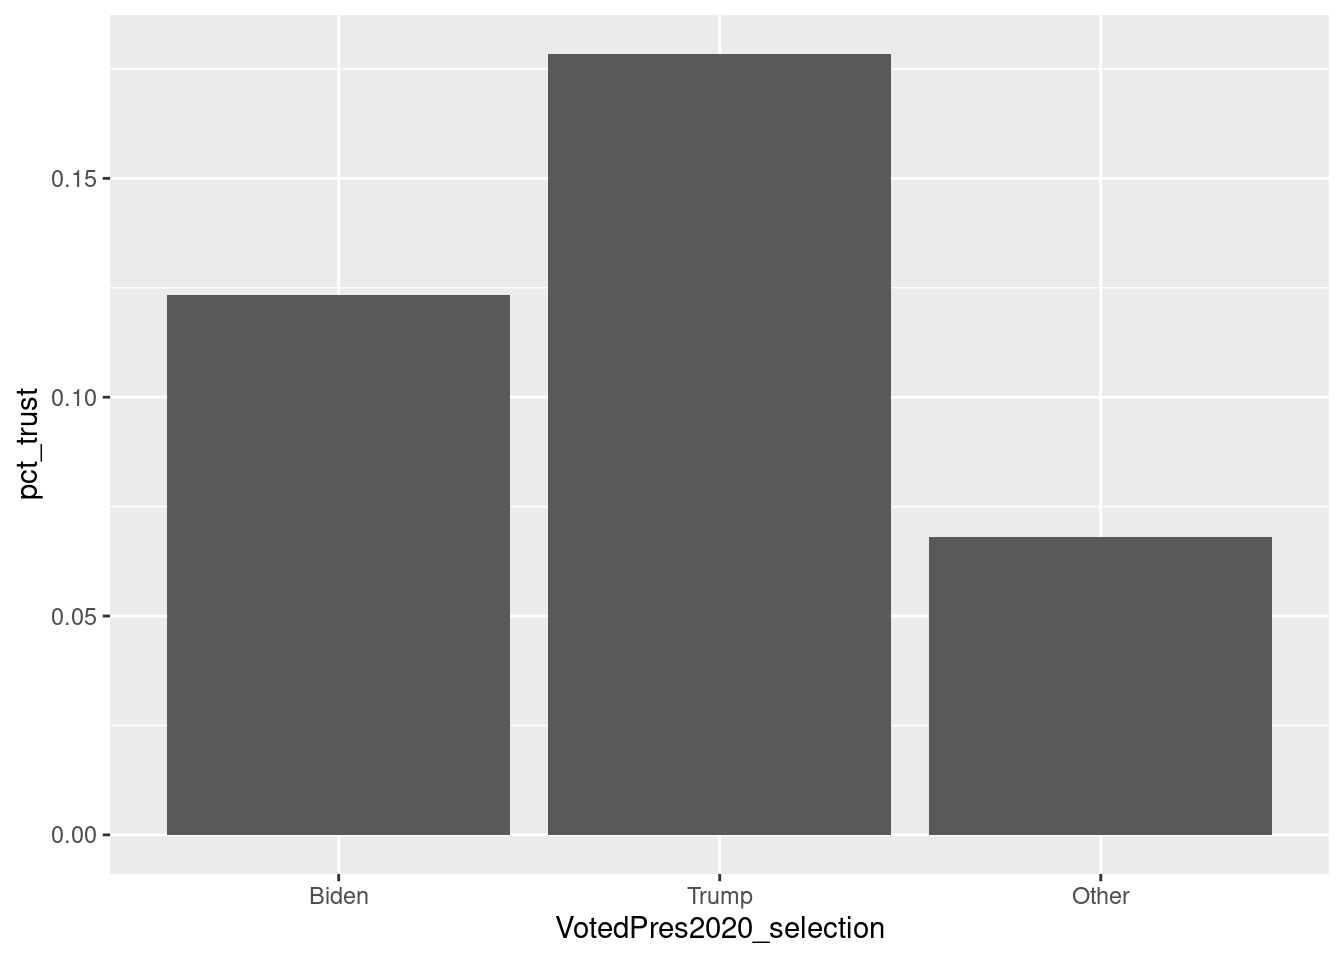
\includegraphics{bookdown_files/figure-latex/results-plot1-1} \caption{Bar chart of trust in government by chosen 2020 presidential candidate}\label{fig:results-plot1}
\end{figure}

This is a great starting point: we observe that a higher percentage of people stating they usually trust the government among those who voted for Trump compared to those who voted for Biden or other candidates. Now, what if we want to introduce color to better differentiate the three groups? We can add \texttt{fill} under \texttt{aesthetics}, indicating that we want to use distinct values of \texttt{VotedPres2020\_selection} to color the bars. In this instance, Biden and Trump will be displayed in different colors.

\begin{Shaded}
\begin{Highlighting}[]
\NormalTok{pcolor }\OtherTok{\textless{}{-}}\NormalTok{ anes\_des\_der }\SpecialCharTok{\%\textgreater{}\%}
  \FunctionTok{ggplot}\NormalTok{(}\FunctionTok{aes}\NormalTok{(}
    \AttributeTok{x =}\NormalTok{ VotedPres2020\_selection,}
    \AttributeTok{y =}\NormalTok{ pct\_trust,}
    \AttributeTok{fill =}\NormalTok{ VotedPres2020\_selection}
\NormalTok{  )) }\SpecialCharTok{+}
  \FunctionTok{geom\_bar}\NormalTok{(}\AttributeTok{stat =} \StringTok{"identity"}\NormalTok{)}

\NormalTok{pcolor}
\end{Highlighting}
\end{Shaded}

\begin{figure}
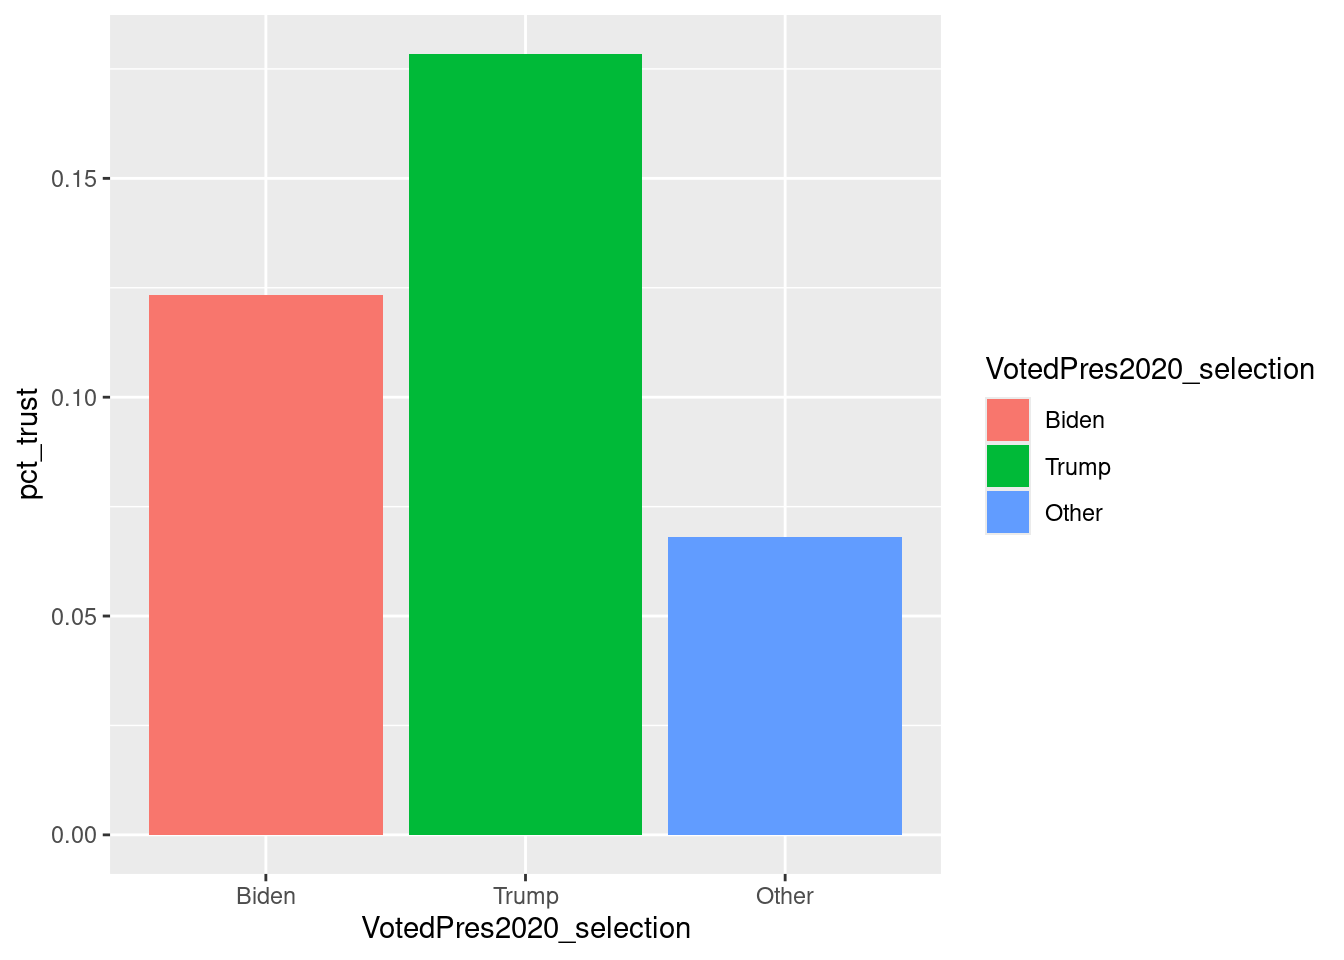
\includegraphics{bookdown_files/figure-latex/results-plot2-1} \caption{Bar chart of trust in government by chosen 2020 presidential candidate with colors}\label{fig:results-plot2}
\end{figure}

Let's say we wanted to follow proper statistical analysis practice and incorporate variability in our plot. We can add another geom, \texttt{geom\_errorbar()}, to display the confidence intervals on top of our existing \texttt{geom\_bar()} layer. We can add the layer using a plus sign \texttt{+}.

\begin{Shaded}
\begin{Highlighting}[]
\NormalTok{pcol\_error }\OtherTok{\textless{}{-}}\NormalTok{ anes\_des\_der }\SpecialCharTok{\%\textgreater{}\%}
  \FunctionTok{ggplot}\NormalTok{(}\FunctionTok{aes}\NormalTok{(}
    \AttributeTok{x =}\NormalTok{ VotedPres2020\_selection,}
    \AttributeTok{y =}\NormalTok{ pct\_trust,}
    \AttributeTok{fill =}\NormalTok{ VotedPres2020\_selection}
\NormalTok{  )) }\SpecialCharTok{+}
  \FunctionTok{geom\_bar}\NormalTok{(}\AttributeTok{stat =} \StringTok{"identity"}\NormalTok{) }\SpecialCharTok{+}
  \FunctionTok{geom\_errorbar}\NormalTok{(}
    \FunctionTok{aes}\NormalTok{(}
      \AttributeTok{ymin =}\NormalTok{ pct\_trust\_low,}
      \AttributeTok{ymax =}\NormalTok{ pct\_trust\_upp}
\NormalTok{    ),}
    \AttributeTok{width =}\NormalTok{ .}\DecValTok{2}
\NormalTok{  )}

\NormalTok{pcol\_error}
\end{Highlighting}
\end{Shaded}

\begin{figure}
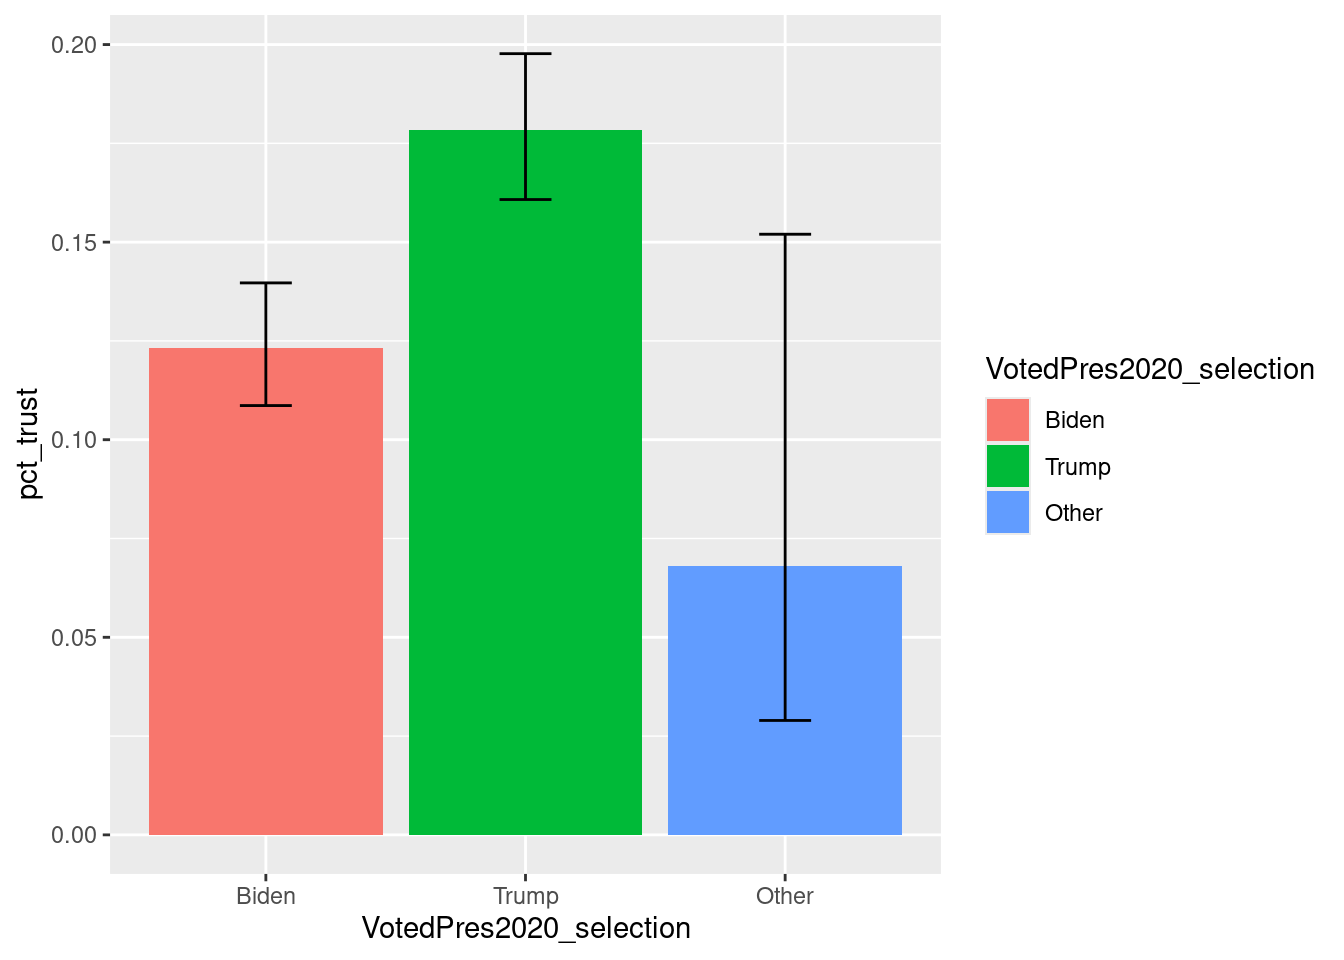
\includegraphics{bookdown_files/figure-latex/results-plot3-1} \caption{Bar chart of trust in government by chosen 2020 presidential candidate with colors and error bars}\label{fig:results-plot3}
\end{figure}

We can continue adding to our plot until we achieve our desired look. For example, we can eliminate the color legend as it doesn't contribute meaningful information with \texttt{guides(fill\ =\ "none")}. We can specify specific colors for \texttt{fill} using \texttt{scale\_fill\_manual()}. Inside the function, we provide a vector of values corresponding to the colors in our plot. These values are hexadecimal (hex) color codes, denoted by a leading pound sign \texttt{\#} followed by six letters or numbers. The hex code \texttt{\#0b3954} used below is a dark blue. There are many tools online that help pick hex codes, such as \href{https://htmlcolorcodes.com/}{htmlcolorcodes.com/}.

\begin{Shaded}
\begin{Highlighting}[]
\NormalTok{pfull }\OtherTok{\textless{}{-}}
\NormalTok{  anes\_des\_der }\SpecialCharTok{\%\textgreater{}\%}
  \FunctionTok{ggplot}\NormalTok{(}\FunctionTok{aes}\NormalTok{(}
    \AttributeTok{x =}\NormalTok{ VotedPres2020\_selection,}
    \AttributeTok{y =}\NormalTok{ pct\_trust,}
    \AttributeTok{fill =}\NormalTok{ VotedPres2020\_selection}
\NormalTok{  )) }\SpecialCharTok{+}
  \FunctionTok{geom\_bar}\NormalTok{(}\AttributeTok{stat =} \StringTok{"identity"}\NormalTok{) }\SpecialCharTok{+}
  \FunctionTok{geom\_errorbar}\NormalTok{(}
    \FunctionTok{aes}\NormalTok{(}
      \AttributeTok{ymin =}\NormalTok{ pct\_trust\_low,}
      \AttributeTok{ymax =}\NormalTok{ pct\_trust\_upp}
\NormalTok{    ),}
    \AttributeTok{width =}\NormalTok{ .}\DecValTok{2}
\NormalTok{  ) }\SpecialCharTok{+}
  \FunctionTok{scale\_fill\_manual}\NormalTok{(}\AttributeTok{values =} \FunctionTok{c}\NormalTok{(}\StringTok{"\#0b3954"}\NormalTok{, }\StringTok{"\#bfd7ea"}\NormalTok{, }\StringTok{"\#8d6b94"}\NormalTok{)) }\SpecialCharTok{+}
  \FunctionTok{xlab}\NormalTok{(}\StringTok{"Election choice (2020)"}\NormalTok{) }\SpecialCharTok{+}
  \FunctionTok{ylab}\NormalTok{(}\StringTok{"Usually trust the government"}\NormalTok{) }\SpecialCharTok{+}
  \FunctionTok{scale\_y\_continuous}\NormalTok{(}\AttributeTok{labels =}\NormalTok{ scales}\SpecialCharTok{::}\NormalTok{percent) }\SpecialCharTok{+}
  \FunctionTok{guides}\NormalTok{(}\AttributeTok{fill =} \StringTok{"none"}\NormalTok{) }\SpecialCharTok{+}
  \FunctionTok{labs}\NormalTok{(}
    \AttributeTok{title =} \StringTok{"Percent of voters who usually trust the government}
\StringTok{       by chosen 2020 presidential candidate"}\NormalTok{,}
    \AttributeTok{caption =} \StringTok{"Source: American National Election Studies, 2020"}
\NormalTok{  )}

\NormalTok{pfull}
\end{Highlighting}
\end{Shaded}

\begin{figure}
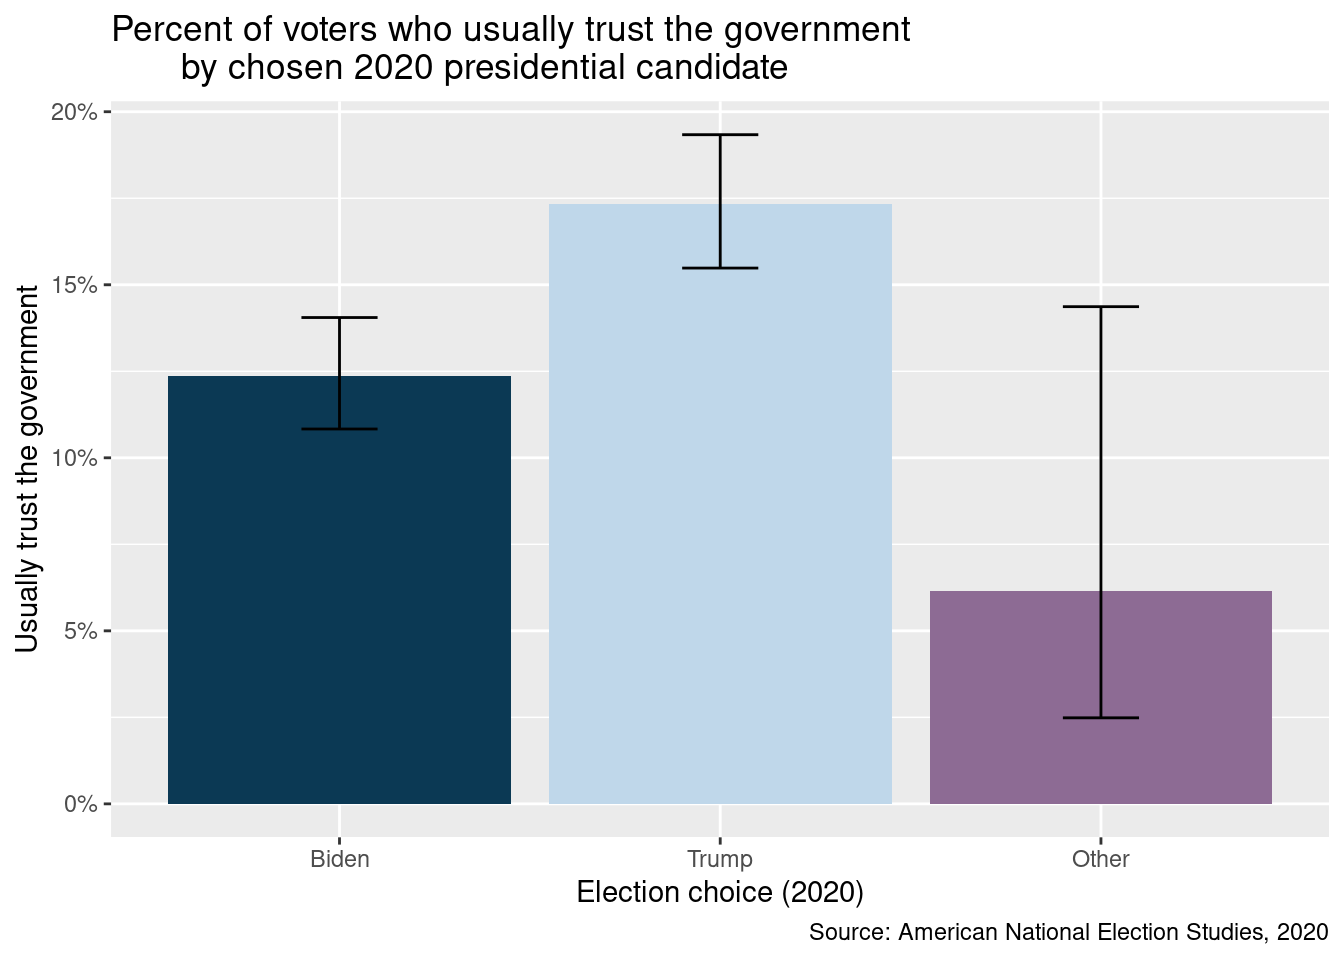
\includegraphics{bookdown_files/figure-latex/results-plot4-1} \caption{Bar chart of trust in government by chosen 2020 presidential candidate with colors, labels, error bars, and title}\label{fig:results-plot4}
\end{figure}

What we've explored in this section are just the foundational aspects of \{ggplot2\}, and the capabilities of this package extend far beyond what we've covered. Advanced features such as annotation, faceting, and theming allow for more sophisticated and customized visualizations. The book \citet{wickham2023ggplot2} is a comprehensive guide to learning more about this powerful tool.

\hypertarget{c09-reprex-data}{%
\chapter{Reproducible research}\label{c09-reprex-data}}

\hypertarget{introduction-7}{%
\section{Introduction}\label{introduction-7}}

Reproducing a data analysis's results is a crucial aspect of any research. First, reproducibility serves as a form of quality assurance. If we pass an analysis project to another person, they should be able to run the entire project from start to finish and obtain the same results. They can critically assess the methodology and code while detecting potential errors. Another goal of reproducibility is enabling the verification of our analysis. When someone else is able to check our results, it ensures the integrity of the analyses by determining that the conclusions are not dependent on a particular person running the code or workflow on a particular day or in a particular environment.

Not only is reproducibility a key component in ethical and accurate research, but it is also a requirement for many scientific journals. For example, the Journal of Survey Statistics and Methodology (JSSAM) and Public Opinion Quarterly (POQ) require authors to make code, data, and methodology transparent and accessible to other researchers who wish to verify or build on existing work.

Reproducible research requires that the key components of analysis are available, discoverable, documented, and shared with others. The four main components that we should consider are:

\begin{itemize}
\tightlist
\item
  \textbf{Code}: source code used for data cleaning, analysis, modeling, and reporting
\item
  \textbf{Data}: raw data used in the workflow, or if data is sensitive or proprietary, as much data as possible that would allow others to run our workflow (e.g., access to a restricted use file (RUF))
\item
  \textbf{Environment}: environment of the project, including the R version, packages, operating system, and other dependencies used in the analysis
\item
  \textbf{Methodology}: analysis methodology, including rationale behind decisions, interpretations, and assumptions
\end{itemize}

In Chapter \ref{c08-communicating-results}, we briefly mention how each of these is important to include in the methodology report and when communicating the findings of a study. However, to be transparent and effective researchers, we need to ensure we not only discuss these through text but also provide files and additional information when requested. Often, when starting a project, analysts will dive into the data and make decisions as they go without full documentation, which can be challenging if we need to go back and make changes or understand even what we did a few months ago. It benefits other analysts and potentially our future selves to better document everything from the start. The good news is that many tools, practices, and project management techniques make survey analysis projects easy to reproduce. For best results, analysts should decide which techniques and tools will be used before starting a project (or very early on).

This chapter covers some of our suggestions for tools and techniques we can use in projects. This list is not comprehensive but aims to provide a starting point for those looking to create a reproducible workflow.

\hypertarget{project-based-workflows}{%
\section{Project-based workflows}\label{project-based-workflows}}

We recommend a project-based workflow for analysis projects as described by \citet{wickham2023r4ds}. A project-based workflow maintains a ``source of truth'' for our analyses. It helps with file system discipline by putting everything related to a project in a designated folder. Since all associated files are in a single location, they are easy to find and organize. When we reopen the project, we can recreate the environment in which we originally ran the code to reproduce our results.

The RStudio IDE has built-in support for projects. When we create a project in RStudio, it creates a \texttt{.Rproj} file that store settings specific to that project. Once we have created a project, we can create folders that help us organize our workflow. For example, a project directory could look like this:

\begin{verbatim}
| anes_analysis/
  | anes_analysis.Rproj
  | README.md
  | codebooks
    | codebook2020.pdf
    | codebook2016.pdf
  | rawdata
    | anes2020_raw.csv
    | anes2016_raw.csv
  | scripts
    | data-prep.R
  | data
    | anes2020_clean.csv
    | anes2016_clean.csv
  | report
    | anes_report.Rmd
    | anes_report.html
    | anes_report.pdf
\end{verbatim}

In a project-based workflow, all paths are relative and, by default, relative to the project's folder. By using relative paths, others can open and run our files even if their directory configuration differs from ours. The \{here\} package enables easy file referencing, and we can start with using the \texttt{here::here()} function to build the path for loading or saving data. Below, we ask R to read the CSV file \texttt{anes\_2020.csv} in the project directory's \texttt{data} folder:

\begin{Shaded}
\begin{Highlighting}[]
\NormalTok{anes }\OtherTok{\textless{}{-}}
  \FunctionTok{read\_csv}\NormalTok{(here}\SpecialCharTok{::}\FunctionTok{here}\NormalTok{(}\StringTok{"data"}\NormalTok{, }\StringTok{"anes2020\_clean.csv"}\NormalTok{))}
\end{Highlighting}
\end{Shaded}

The combination of projects and the \{here\} package keep all associated files in an organized manner. This workflow makes it more likely that our analyses can be reproduced by us or our colleagues.

\hypertarget{functions-and-packages}{%
\section{Functions and packages}\label{functions-and-packages}}

We may find ourselves repeating ourselves in our script, and the chances of errors increases whenever we copy and paste our code. By creating a function, we can create a consistent set of commands that reduce the likelihood of mistakes. Functions also organize our code, improve the code readability, and allow others to execute the same commands. Throughout this book, we have created functions, such as in Chapter \ref{c13-ncvs-vignette}, to run sequences of rename, filter, group\_by, and summarize statements across different variables. The function helps us avoid overlooking necessary steps.

A package is made up of a collection of functions. If we find ourselves sharing functions with others to replicate the same series of commands in a separate project, creating a package can be a useful tool for sharing the code along with data and documentation.

\hypertarget{version-control-with-git}{%
\section{Version control with Git}\label{version-control-with-git}}

Often, a survey analysis project produces a lot of code. Keeping track of the latest version can become challenging as files evolve throughout a project. If a team of analysts is working on the same script, someone may use an outdated version, resulting in incorrect results or redundant work.

Version control systems like Git can help alleviate these pains. Git is a system that helps track changes in computer files. Analysts can use Git to follow code evaluation and manage asynchronous work. With Git, it is easy to see any changes made in a script, revert changes, and resolve differences between code versions (called conflicts).

Services such as GitHub or GitLab provide hosting and sharing of files as well as version control with Git. For example, we can visit the GitHub repository for this book (\url{https://github.com/tidy-survey-r/tidy-survey-book}) and see the files that build the book, when they were committed to the repository, and the history of modifications over time.

In addition to code scripts, platforms like GitHub can store data and documentation. They provide a way to maintain a history of data modifications through versioning and timestamps. By saving the data and documentation alongside the code, it becomes easier for others to refer to and access everything they need in one place.

Using version control in analysis projects makes collaboration and maintenance more manageable. For connecting Git with R, we recommend the book \href{https://happygitwithr.com/}{Happy Git and GitHub for the useR} \citep{git-w-R}.

\hypertarget{package-management-with-renv}{%
\section{Package management with \{renv\}}\label{package-management-with-renv}}

Ensuring reproducibility involves not only using version control of code, but also managing the versions of packages. If two people run the same code but use different versions of a package, the results might differ because of changes in those packages. For example, this book currently uses a version of the \{srvyr\} package from GitHub and not from CRAN. This is because the version of \{srvyr\} on CRAN has some bugs (errors) that result in incorrect calculations. The version on GitHub has corrected these errors, so we have asked readers to install the GitHub version to obtain the same results.

One way to handle different package versions is with the \{renv\} package. This package allows researchers to set the versions for each package used and manage package dependencies. Specifically, \{renv\} creates isolated, project-specific environments that record the packages and their versions used in the code. When initiated by a new user, \{renv\} checks whether the installed packages are consistent with the recorded version for the project. If not, it installs the appropriate versions so that others can replicate the project's environment to rerun the code and obtain consistent results.

\hypertarget{r-environments-with-docker}{%
\section{R environments with Docker}\label{r-environments-with-docker}}

Just as different versions of packages can introduce discrepancies or compatibility issues, the version of R can also prevent reproducibility. Tools such as Docker can help with this potential issue by creating isolated environments that define the version of R being used, along with other dependencies and configurations. The entire environment is bundled in a container. The container, defined by a Dockerfile, can be shared so anybody, regardless of their local setup, can run the R code in the same environment.

\hypertarget{workflow-management-with-targets}{%
\section{Workflow management with \{targets\}}\label{workflow-management-with-targets}}

With complex studies involving multiple code files and dependencies, it is important to ensures each step is executed in the intended sequence. We can do this manually, e.g., numbering files to indicate the order or providing detailed documentation on the order. Alternatively, we can automate the process so the code flows sequentially. Making sure that the code runs in the correct order helps ensure that the research is reproducible. Anyone should be able to pick up the set of scripts and get the same results by following the workflow.

The \{targets\} package is growing as a popular workflow manager that documents, automates, and executes complex data workflows with multiple steps and dependencies. With this package, we first define the order of execution for our code, and then it will consistently execute the code in that order each time it is run. One beneficial feature of \{targets\} is that if you change code later in the workflow, only the affected code and its downstream targets (i.e., the subsequent code files) are re-executed when we change a script. The \{targets\} package also provides interactive progress monitoring and reporting, allowing us to track the status and progress of our analysis pipeline.

\hypertarget{documentation-with-quarto-and-r-markdown}{%
\section{Documentation with Quarto and R Markdown}\label{documentation-with-quarto-and-r-markdown}}

Tools like Quarto and R Markdown aid in reproducibility by creating documents that weave together code, text, and results. We can present analysis results alongside the report's narrative, so there's no need to copy and paste code output into the final documentation. By eliminating manual steps, we can reduce the chances of errors in the final output.

Quarto and R Markdown documents also allow users to re-execute the underlying code when needed. Another analyst can see the steps we took, follow the scripts, and recreate the report. We can include details about our work in one place thanks to the combination of text and code, making our work transparent and easier to verify.

\hypertarget{parameterization}{%
\subsection{Parameterization}\label{parameterization}}

Another useful feature of Quarto and R Markdown is the ability to reduce repetitive code by parameterizing the files. Parameters can control various aspects of the analysis, such as dates, geography, or other analysis variables. We can define and modify these parameters to explore different scenarios or inputs. For example, suppose we start by creating a document that provides survey analysis results for North Carolina but then later decide we want to look at another state. In that case, we can define a \texttt{state} parameter and rerun the same analysis for a state like Washington without having to edit the code throughout the document.

Parameters can be defined in the header or code chunks of our Quarto or R Markdown documents and easily be modified and documented. We reduce errors that may occur by manually editing code throughout the script, and offer a flexible way for others to replicate the analysis and explore variations.

\hypertarget{other-tips-for-reproducibility}{%
\section{Other tips for reproducibility}\label{other-tips-for-reproducibility}}

\hypertarget{random-number-seeds}{%
\subsection{Random number seeds}\label{random-number-seeds}}

Some tasks in survey analysis require randomness, such as imputation, model training, or creating random samples. By default, the random numbers generated by R change each time we rerun the code, making it difficult to reproduce the same results. By ``setting the seed,'' we can control the randomness and ensure that the random numbers remain consistent whenever we rerun the code. Others can use the same seed value to reproduce our random numbers and achieve the same results.

In R, we can use the \texttt{set.seed()} function to control the randomness in our code. Set a seed value by providing an integer to the function:

\begin{Shaded}
\begin{Highlighting}[]
\FunctionTok{set.seed}\NormalTok{(}\DecValTok{999}\NormalTok{)}

\FunctionTok{runif}\NormalTok{(}\DecValTok{5}\NormalTok{)}
\end{Highlighting}
\end{Shaded}

The \texttt{runif()} function generates five random numbers from a uniform distribution. Since the seed is set to \texttt{999}, running \texttt{runif()} multiple times will always produce the same sequence:

\begin{verbatim}
[1] 0.38907138 0.58306072 0.09466569 0.85263123 0.78674676
\end{verbatim}

The choice of the seed number is up to the analyst. For example, this could be the date (\texttt{20240102}) or time of day (\texttt{1056}) when the analysis was first conducted, a phone number (\texttt{8675309}), or the first few numbers that come to mind (\texttt{369}). As long as the seed is set for a given analysis, the actual number is up to the analyst to decide. It is important to note that \texttt{set.seed()} should be used \emph{before} random number generation. Run it once per program, and the seed will be applied to the entire script. We recommend setting the seed at the beginning of a script, where libraries are loaded.

\hypertarget{descriptive-names-and-labels}{%
\subsection{Descriptive names and labels}\label{descriptive-names-and-labels}}

Using descriptive variable names or labeling data can also assist with reproducible research. For example, in the ANES data, the variable names in the raw data all start with \texttt{V20} and are a string of numbers. To make things easier to reproduce, we opted to change the variable names to be more descriptive of what they contained (e.g., \texttt{Age}). This can also be done with the data values themselves. One way to accomplish this is by creating factors for categorical data, which can ensure that we know that a value of \texttt{1} really means \texttt{Female}, for example. There are other ways of handling this, such as attaching labels to the data instead of recoding variables to be descriptive (see Chapter \ref{c11-missing-data}). As with random number seeds, the exact method is up to the analyst, but providing this information can help ensure our research is reproducible.

\hypertarget{summary}{%
\section{Summary}\label{summary}}

We can promote accuracy and verification of results by making our analysis reproducible. There are various tools and guides available to help you achieve reproducibility in your work, a few of which were described in this chapter. Here are additional resources to explore:

\begin{itemize}
\tightlist
\item
  R for Data Science chapter on project-based workflows: \url{https://r4ds.hadley.nz/workflow-scripts.html\#projects}
\item
  Building reproducible analytical pipelines with R by Bruno Rodrigues: \url{https://raps-with-r.dev/}
\item
  Posit Solutions Site page on reproducible environments: \url{https://solutions.posit.co/envs-pkgs/environments/}
\end{itemize}

\hypertarget{part-real-life-data}{%
\part{Real life data}\label{part-real-life-data}}

\hypertarget{c10-specifying-sample-designs}{%
\chapter{Specifying sample designs and replicate weights in \{srvyr\}}\label{c10-specifying-sample-designs}}

\begin{prereqbox}{Prerequisites}

For this chapter, load the following packages:

\begin{Shaded}
\begin{Highlighting}[]
\FunctionTok{library}\NormalTok{(tidyverse)}
\FunctionTok{library}\NormalTok{(survey)}
\FunctionTok{library}\NormalTok{(srvyr)}
\FunctionTok{library}\NormalTok{(srvyrexploR)}
\end{Highlighting}
\end{Shaded}

To help explain the different types of sample designs, this chapter will use the \texttt{api} and \texttt{scd} data that are included in the \{survey\} package:

\begin{Shaded}
\begin{Highlighting}[]
\FunctionTok{data}\NormalTok{(api)}
\FunctionTok{data}\NormalTok{(scd)}
\end{Highlighting}
\end{Shaded}

This chapter uses data from the Residential Energy Consumption Survey (RECS) - both 2015 and 2020, so we will use the following code to load the RECS data from the \{srvyr.data\} package:

\begin{Shaded}
\begin{Highlighting}[]
\FunctionTok{data}\NormalTok{(recs\_2015)}
\FunctionTok{data}\NormalTok{(recs\_2020)}
\end{Highlighting}
\end{Shaded}

\end{prereqbox}

\hypertarget{introduction-8}{%
\section{Introduction}\label{introduction-8}}

The primary reason for using packages like \{survey\} and \{srvyr\} is to account for the sampling design or replicate weights into estimates. By incorporating the sampling design or replicate weights, precision estimates (e.g., standard errors and confidence intervals) are appropriately calculated.

In this chapter, we will introduce common sampling designs and common types of replicate weights, the mathematical methods for calculating estimates and standard errors for a given sampling design, and the R syntax to specify the sampling design or replicate weights. While we will show the math behind the estimates, the functions in these packages will do the calculation. To deeply understand the math and the derivation, refer to \citet{pennstate506}, \citet{sarndal2003model}, \citet{wolter2007introduction}, or \citet{fuller2011sampling} (these are listed in order of increasing statistical rigorousness).

The general process for estimation in the \{srvyr\} package is to:

\begin{enumerate}
\def\labelenumi{\arabic{enumi}.}
\item
  Create a \texttt{tbl\_svy} object (a survey object) using: \texttt{as\_survey\_design()} or \texttt{as\_survey\_rep()}
\item
  Subset data (if needed) using \texttt{filter()} (subpopulations)
\item
  Specify domains of analysis using \texttt{group\_by()}
\item
  Within \texttt{summarize()}, specify variables to calculate, including means, totals, proportions, quantiles, and more
\end{enumerate}

This chapter includes details on the first step - creating the survey object. Once this survey object is created, it can be used in the other steps (detailed in chapters \ref{c05-descriptive-analysis} through \ref{c07-modeling}) to account for the complex survey design.

\hypertarget{common-sampling-designs}{%
\section{Common sampling designs}\label{common-sampling-designs}}

A sampling design is the method used to draw a sample. Both logistical and statistical elements are considered when developing a sampling design. When specifying a sampling design in R, the levels of sampling are specified along with the weights. The weight for each record is constructed so that the particular record represents that many units in the population. For example, in a survey of 6th-grade students in the United States, the weight associated with each responding student reflects how many 6th grade students across the country that record represents. Generally, the weights represent the inverse of the probability of selection such that the sum of the weights corresponds to the total population size, although some studies may have the sum of the weights equal to the number of respondent records.

Some common terminology across the designs are:

\begin{itemize}
\tightlist
\item
  \textbf{sample size}, generally denoted as \(n\), is the number of units selected to be sampled
\item
  \textbf{population size}, generally denoted as \(N\), is the number of units in the target population
\item
  \textbf{sampling frame}, the list of units from which the sample is drawn (see Chapter \ref{c02-overview-surveys} for more information)
\end{itemize}

\hypertarget{simple-random-sample-without-replacement}{%
\subsection{Simple random sample without replacement}\label{simple-random-sample-without-replacement}}

The simple random sample (SRS) without replacement is a sampling design where a fixed sample size is selected from a sampling frame, and every possible subsample has an equal probability of selection. Without replacement refers to the fact that once a sampling unit has been selected, it is removed from the sample frame and cannot be selected again.

\begin{itemize}
\tightlist
\item
  \textbf{Requirements}: The sampling frame must include the entire population.
\item
  \textbf{Advantages}: SRS requires no information about the units apart from contact information.
\item
  \textbf{Disadvantages}: The sampling frame may not be available for the entire population.
\item
  \textbf{Example}: Randomly select students in a university from a roster provided by the registrar's office.
\end{itemize}

\hypertarget{the-math}{%
\subsubsection*{The math}\label{the-math}}


The estimate for the population mean of variable \(y\) is:

\[\bar{y}=\frac{1}{n}\sum_{i=1}^n y_i\]
where \(\bar{y}\) represents the sample mean, \(n\) is the total number of respondents (or observations), and \(y_i\) is each individual value of \(y\).

The estimate of the standard error of the mean is:

\[se(\bar{y})=\sqrt{\frac{s^2}{n}\left( 1-\frac{n}{N} \right)}\] where

\[s^2=\frac{1}{n-1}\sum_{i=1}^n\left(y_i-\bar{y}\right)^2.\]

and \(N\) is the population size. This standard error estimate might look very similar to equations in other applications except for the part on the right side of the equation: \(1-\frac{n}{N}\). This is called the finite population correction (FPC) factor. If the size of the frame, \(N\), is very large in comparison to the sample, the FPC is negligible, so it is often ignored. A common guideline is if the sample is less than 10\% of the population, the FPC is negligible.

To estimate proportions, we define \(x_i\) as the indicator if the outcome is observed. That is, \(x_i=1\) if the outcome is observed, and \(x_i=0\) if the outcome is not observed for respondent \(i\). Then the estimated proportion from an SRS design is:

\[\hat{p}=\frac{1}{n}\sum_{i=1}^n x_i \]
and the estimated standard error of the proportion is:

\[se(\hat{p})=\sqrt{\frac{\hat{p}(1-\hat{p})}{n-1}\left(1-\frac{n}{N}\right)} \]

\hypertarget{the-syntax}{%
\subsubsection*{The syntax}\label{the-syntax}}


If a sample was drawn through SRS and had no nonresponse or other weighting adjustments, in R, specify this design as:

\begin{Shaded}
\begin{Highlighting}[]
\NormalTok{srs1\_des }\OtherTok{\textless{}{-}}\NormalTok{ dat }\SpecialCharTok{\%\textgreater{}\%}
 \FunctionTok{as\_survey\_design}\NormalTok{(}\AttributeTok{fpc =}\NormalTok{ fpcvar)}
\end{Highlighting}
\end{Shaded}

where \texttt{dat} is a tibble or data.frame with the survey data, and \texttt{fpcvar} is a variable in the data indicating the sampling frame's size (this variable will have the same value for all cases in an SRS design). If the frame is very large, sometimes the frame size is not provided. In that case, the FPC is not needed, and specify the design as:

\begin{Shaded}
\begin{Highlighting}[]
\NormalTok{srs2\_des }\OtherTok{\textless{}{-}}\NormalTok{ dat }\SpecialCharTok{\%\textgreater{}\%}
 \FunctionTok{as\_survey\_design}\NormalTok{()}
\end{Highlighting}
\end{Shaded}

If some post-survey adjustments were implemented and the weights are not all equal, specify the design as:

\begin{Shaded}
\begin{Highlighting}[]
\NormalTok{srs3\_des }\OtherTok{\textless{}{-}}\NormalTok{ dat }\SpecialCharTok{\%\textgreater{}\%}
 \FunctionTok{as\_survey\_design}\NormalTok{(}\AttributeTok{weights =}\NormalTok{ wtvar, }
                  \AttributeTok{fpc =}\NormalTok{ fpcvar)}
\end{Highlighting}
\end{Shaded}

where \texttt{wtvar} is a variable in the data indicating the weight for each case. Again, the FPC can be omitted if it is unnecessary because the frame is large compared to the sample size.

\hypertarget{example-2}{%
\subsubsection*{Example}\label{example-2}}


The \{survey\} package in R provides some example datasets that we will use throughout this chapter. The documentation provides detailed information about the variables. One of the example datasets we will use is from the Academic Performance Index (API). The API was a program administered by the California Department of Education, and the \{survey\} package includes a population file (sample frame) of all schools with at least 100 students and several different samples pulled from that data using different sampling methods. For this first example, we will use the \texttt{apisrs} dataset, which contains an SRS of 200 schools. For printing purposes, we create a new dataset called \texttt{apisrs\_slim}, which sorts the data by the school district and school ID and subsets the data to only a few columns. The SRS sample data is illustrated below:

\begin{Shaded}
\begin{Highlighting}[]
\NormalTok{apisrs\_slim }\OtherTok{\textless{}{-}}
\NormalTok{  apisrs }\SpecialCharTok{\%\textgreater{}\%}
  \FunctionTok{as\_tibble}\NormalTok{() }\SpecialCharTok{\%\textgreater{}\%}
  \FunctionTok{arrange}\NormalTok{(dnum, snum) }\SpecialCharTok{\%\textgreater{}\%}
  \FunctionTok{select}\NormalTok{(cds, dnum, snum, dname, sname, fpc, pw)}

\NormalTok{apisrs\_slim}
\end{Highlighting}
\end{Shaded}

\begin{verbatim}
## # A tibble: 200 x 7
##    cds             dnum  snum dname                   sname    fpc    pw
##    <chr>          <int> <dbl> <chr>                   <chr>  <dbl> <dbl>
##  1 19642126061220     1  1121 ABC Unified             Haske~  6194  31.0
##  2 19642126066716     1  1124 ABC Unified             Stowe~  6194  31.0
##  3 36675876035174     5  3895 Adelanto Elementary     Adela~  6194  31.0
##  4 33669776031512    19  3347 Alvord Unified          Arlan~  6194  31.0
##  5 33669776031595    19  3352 Alvord Unified          Wells~  6194  31.0
##  6 31667876031033    39  3271 Auburn Union Elementary Cain ~  6194  31.0
##  7 19642876011407    42  1169 Baldwin Park Unified    Deanz~  6194  31.0
##  8 19642876011464    42  1175 Baldwin Park Unified    Heath~  6194  31.0
##  9 19642956011589    48  1187 Bassett Unified         Erwin~  6194  31.0
## 10 41688586043392    49  4948 Bayshore Elementary     Baysh~  6194  31.0
## # i 190 more rows
\end{verbatim}

Table \ref{tab:apidata} provides details on all the variables in this dataset.

\begin{longtable}[]{@{}cl@{}}
\caption{\label{tab:apidata} Overview of Variables in \texttt{api} Data}\tabularnewline
\toprule\noalign{}
Variable Name & Description \\
\midrule\noalign{}
\endfirsthead
\toprule\noalign{}
Variable Name & Description \\
\midrule\noalign{}
\endhead
\bottomrule\noalign{}
\endlastfoot
\texttt{cds} & Unique identifier for each school \\
\texttt{dnum} & School district identifier within county \\
\texttt{snum} & School identifier within district \\
\texttt{dname} & District Name \\
\texttt{sname} & School Name \\
\texttt{fpc} & Finite population correction factor (FPC) \\
\texttt{pw} & Weight \\
\end{longtable}

To create the \texttt{tbl\_survey} object for this SRS data, the design should be specified as follows:

\begin{Shaded}
\begin{Highlighting}[]
\NormalTok{apisrs\_des }\OtherTok{\textless{}{-}}\NormalTok{ apisrs\_slim }\SpecialCharTok{\%\textgreater{}\%}
  \FunctionTok{as\_survey\_design}\NormalTok{(}
    \AttributeTok{weights =}\NormalTok{ pw,}
    \AttributeTok{fpc =}\NormalTok{ fpc}
\NormalTok{  )}

\NormalTok{apisrs\_des}
\end{Highlighting}
\end{Shaded}

\begin{verbatim}
## Independent Sampling design
## Called via srvyr
## Sampling variables:
##   - ids: `1` 
##   - fpc: fpc 
##   - weights: pw 
## Data variables: 
##   - cds (chr), dnum (int), snum (dbl), dname (chr), sname (chr), fpc
##     (dbl), pw (dbl)
\end{verbatim}

In the printed design object above, the design is described as an ``Independent Sampling design,'' which is another term for SRS. The ids are specified as \texttt{1}, which means there is no clustering (a topic described in Section \ref{samp-cluster}), the FPC variable is indicated, and the weights are indicated. We can also look at the summary of the design object, and see the distribution of the probabilities (inverse of the weights) along with the population size and a list of the variables in the dataset.

\begin{Shaded}
\begin{Highlighting}[]
\FunctionTok{summary}\NormalTok{(apisrs\_des)}
\end{Highlighting}
\end{Shaded}

\begin{verbatim}
## Independent Sampling design
## Called via srvyr
## Probabilities:
##    Min. 1st Qu.  Median    Mean 3rd Qu.    Max. 
##  0.0323  0.0323  0.0323  0.0323  0.0323  0.0323 
## Population size (PSUs): 6194 
## Data variables:
## [1] "cds"   "dnum"  "snum"  "dname" "sname" "fpc"   "pw"
\end{verbatim}

\hypertarget{simple-random-sample-with-replacement}{%
\subsection{Simple random sample with replacement}\label{simple-random-sample-with-replacement}}

Similar to the SRS design, the simple random sample with replacement (SRSWR) design randomly selects the sample from the entire sampling frame. However, while SRS removes sampled units before selecting again, the SRSWR instead replaces each sampled unit before drawing again, so units can be selected more than once.

\begin{itemize}
\tightlist
\item
  \textbf{Requirements}: The sampling frame must include the entire population.
\item
  \textbf{Advantages}: SRSWR requires no information about the units apart from contact information.
\item
  \textbf{Disadvantages}:

  \begin{itemize}
  \tightlist
  \item
    The sampling frame may not be available for the entire population.
  \item
    Units can be selected more than once, resulting in a smaller realized sample size because receiving duplicate information from a single respondent does not provide additional information.
  \item
    For small populations, SRSWR has larger standard errors than SRS designs.
  \end{itemize}
\item
  \textbf{Example}: A professor puts all students' names on paper slips and selects them randomly to ask students questions, but the professor replaces the paper after calling on the student so they can be selected again at any time.
\end{itemize}

In general for surveys, using an SRS design (without replacement) is preferred as we do not want respondents to answer a survey more than once.

\hypertarget{the-math-1}{%
\subsubsection*{The math}\label{the-math-1}}


The estimate for the population mean of variable \(y\) is:

\[\bar{y}=\frac{1}{n}\sum_{i=1}^n y_i\]

and the estimate of the standard error of mean is:

\[se(\bar{y})=\sqrt{\frac{s^2}{n}}\] where

\[s^2=\frac{1}{n-1}\sum_{i=1}^n\left(y_i-\bar{y}\right)^2.\]
To calculate the estimated proportion, we define \(x_i\) as the indicator that the outcome is observed (as we did with SRS):

\[\hat{p}=\frac{1}{n}\sum_{i=1}^n x_i \]
and the estimated standard error of the proportion is:

\[se(\hat{p})=\sqrt{\frac{\hat{p}(1-\hat{p})}{n}} \]

\hypertarget{the-syntax-1}{%
\subsubsection*{The syntax}\label{the-syntax-1}}


If we had a sample that was drawn through SRSWR and had no nonresponse or other weighting adjustments, in R, we should specify this design as:

\begin{Shaded}
\begin{Highlighting}[]
\NormalTok{srswr1\_des }\OtherTok{\textless{}{-}}\NormalTok{ dat }\SpecialCharTok{\%\textgreater{}\%}
 \FunctionTok{as\_survey\_design}\NormalTok{()}
\end{Highlighting}
\end{Shaded}

where \texttt{dat} is a tibble or data.frame containing our survey data. This syntax is the same as a SRS design, except a finite population correction (FPC) is not included. This is because when you claculate a sample with replacement, the population pool to select from is no longer finite, so a correction is not needed. Therefore, with large populations where the FPC is negligble, the underlying formulas for SRS and SRSWR designs are the same.

If some post-survey adjustments were implemented and the weights are not all equal, specify the design as:

\begin{Shaded}
\begin{Highlighting}[]
\NormalTok{srswr2\_des }\OtherTok{\textless{}{-}}\NormalTok{ dat }\SpecialCharTok{\%\textgreater{}\%}
 \FunctionTok{as\_survey\_design}\NormalTok{(}\AttributeTok{weights =}\NormalTok{ wtvar)}
\end{Highlighting}
\end{Shaded}

where \texttt{wtvar} is the variable for the weight on the data.

\hypertarget{example-3}{%
\subsubsection*{Example}\label{example-3}}


The \{survey\} package does not include an example of SRSWR, so to illustrate this design we need to create an example. We use the api population data provided by the \{survey\} package \texttt{apipop} and select a sample of 200 cases using the \texttt{slice\_sample()} function from the tidyverse. One of the arguments in the \texttt{slice\_sample()} function is \texttt{replace}. If \texttt{replace=TRUE}, then we are conducting a SRSWR. We then calculate selection weights as the inverse of the probability of selection and call this new dataset \texttt{apisrswr}.

\begin{Shaded}
\begin{Highlighting}[]
\FunctionTok{set.seed}\NormalTok{(}\DecValTok{409963}\NormalTok{)}

\NormalTok{apisrswr }\OtherTok{\textless{}{-}}\NormalTok{ apipop }\SpecialCharTok{\%\textgreater{}\%}
  \FunctionTok{as\_tibble}\NormalTok{() }\SpecialCharTok{\%\textgreater{}\%}
  \FunctionTok{slice\_sample}\NormalTok{(}\AttributeTok{n =} \DecValTok{200}\NormalTok{, }\AttributeTok{replace =} \ConstantTok{TRUE}\NormalTok{) }\SpecialCharTok{\%\textgreater{}\%}
  \FunctionTok{select}\NormalTok{(cds, dnum, snum, dname, sname) }\SpecialCharTok{\%\textgreater{}\%}
  \FunctionTok{mutate}\NormalTok{(}
    \AttributeTok{weight =} \FunctionTok{nrow}\NormalTok{(apipop) }\SpecialCharTok{/} \DecValTok{200}
\NormalTok{  )}

\FunctionTok{head}\NormalTok{(apisrswr)}
\end{Highlighting}
\end{Shaded}

\begin{verbatim}
## # A tibble: 6 x 6
##   cds             dnum  snum dname                    sname       weight
##   <chr>          <int> <dbl> <chr>                    <chr>        <dbl>
## 1 43696416060065   533  5348 Palo Alto Unified        Jordan (Da~   31.0
## 2 07618046005060   650   509 San Ramon Valley Unified Alamo Elem~   31.0
## 3 19648086085674   457  2134 Montebello Unified       La Merced ~   31.0
## 4 07617056003719   346   377 Knightsen Elementary     Knightsen ~   31.0
## 5 19650606023022   744  2351 Torrance Unified         Carr (Evel~   31.0
## 6 01611196090120     6    13 Alameda City Unified     Paden (Wil~   31.0
\end{verbatim}

Because this is a SRS design \emph{with replacement}, there will be duplicates in the data. It is important to keep the duplicates in the data for proper estimation, but for reference we can view the duplicates in the example data we just created.

\begin{Shaded}
\begin{Highlighting}[]
\NormalTok{apisrswr }\SpecialCharTok{\%\textgreater{}\%}
  \FunctionTok{group\_by}\NormalTok{(cds) }\SpecialCharTok{\%\textgreater{}\%}
  \FunctionTok{filter}\NormalTok{(}\FunctionTok{n}\NormalTok{() }\SpecialCharTok{\textgreater{}} \DecValTok{1}\NormalTok{) }\SpecialCharTok{\%\textgreater{}\%}
  \FunctionTok{arrange}\NormalTok{(cds)}
\end{Highlighting}
\end{Shaded}

\begin{verbatim}
## # A tibble: 4 x 6
## # Groups:   cds [2]
##   cds             dnum  snum dname                 sname          weight
##   <chr>          <int> <dbl> <chr>                 <chr>           <dbl>
## 1 15633216008841    41   869 Bakersfield City Elem Chipman Junio~   31.0
## 2 15633216008841    41   869 Bakersfield City Elem Chipman Junio~   31.0
## 3 39686766042782   716  4880 Stockton City Unified Tyler Skills ~   31.0
## 4 39686766042782   716  4880 Stockton City Unified Tyler Skills ~   31.0
\end{verbatim}

We created a weight variable in this example data, which is the inverse of the probability of selection. To specify the sampling design for \texttt{apisrswr}, the following syntax should be used:

\begin{Shaded}
\begin{Highlighting}[]
\NormalTok{apisrswr\_des }\OtherTok{\textless{}{-}}\NormalTok{ apisrswr }\SpecialCharTok{\%\textgreater{}\%}
  \FunctionTok{as\_survey\_design}\NormalTok{(}\AttributeTok{weights =}\NormalTok{ weight)}

\NormalTok{apisrswr\_des}
\end{Highlighting}
\end{Shaded}

\begin{verbatim}
## Independent Sampling design (with replacement)
## Called via srvyr
## Sampling variables:
##   - ids: `1` 
##   - weights: weight 
## Data variables: 
##   - cds (chr), dnum (int), snum (dbl), dname (chr), sname (chr), weight
##     (dbl)
\end{verbatim}

\begin{Shaded}
\begin{Highlighting}[]
\FunctionTok{summary}\NormalTok{(apisrswr\_des)}
\end{Highlighting}
\end{Shaded}

\begin{verbatim}
## Independent Sampling design (with replacement)
## Called via srvyr
## Probabilities:
##    Min. 1st Qu.  Median    Mean 3rd Qu.    Max. 
##  0.0323  0.0323  0.0323  0.0323  0.0323  0.0323 
## Data variables:
## [1] "cds"    "dnum"   "snum"   "dname"  "sname"  "weight"
\end{verbatim}

In the output above, the design object and the object summary are shown. Both note that the sampling is done ``with replacement'' because no FPC was specified. The probabilities, which are derived from the weights, are summarized in the summary.

\hypertarget{stratified-sampling}{%
\subsection{Stratified sampling}\label{stratified-sampling}}

Stratified sampling occurs when a population is divided into mutually exclusive subpopulations (strata), and then samples are selected independently within each stratum.

\begin{itemize}
\tightlist
\item
  \textbf{Requirements}: The sampling frame must include the information to divide the population into groups for every unit.
\item
  \textbf{Advantages}:

  \begin{itemize}
  \tightlist
  \item
    This design ensures sample representation in all subpopulations.
  \item
    If the strata are correlated with survey outcomes, a stratified sample has smaller standard errors compared to a SRS sample of the same size.\\
  \item
    This results in a more efficient design.
  \end{itemize}
\item
  \textbf{Disadvantages}: Auxiliary data may not exist to divide the sampling frame into groups, or the data may be outdated.
\item
  \textbf{Examples}:

  \begin{itemize}
  \tightlist
  \item
    \textbf{Example 1}: A population of North Carolina residents could be separated (stratified) into urban and rural areas, and then a SRS of residents from both rural and urban areas is selected independently. This ensures there are residents from both areas in the sample.
  \item
    \textbf{Example 2}: Law enforcement agencies could be separated (stratified) into the three primary general-purpose categories in the US: local police, sheriff's departments, and state police. A SRS of agencies from each of the three types is then selected independently to ensure all three types of agencies are represented.
  \end{itemize}
\end{itemize}

\hypertarget{the-math-2}{%
\subsubsection*{The math}\label{the-math-2}}


Let \(\bar{y}_h\) be the sample mean for stratum \(h\), \(N_h\) be the population size of stratum \(h\), and \(n_h\) be the sample size of stratum \(h\). Then the estimate for the population mean under stratified SRS sampling is:

\[\bar{y}=\frac{1}{N}\sum_{h=1}^H N_h\bar{y}_h\]
and the estimate of the standard error of \(\bar{y}\) is:

\[se(\bar{y})=\sqrt{\frac{1}{N^2} \sum_{h=1}^H N_h^2 \frac{s_h^2}{n_h}\left(1-\frac{n_h}{N_h}\right)} \]

where
\[s_h^2=\frac{1}{n_h-1}\sum_{i=1}^{n_h}\left(y_{i,h}-\bar{y}_h\right)^2.\]

For estimates of proportions, let \(\hat{p}_h\) be the estimated proportion in stratum \(h\). Then the population proportion estimate is:

\[\hat{p}= \frac{1}{N}\sum_{h=1}^H N_h \hat{p}_h\]

where \(H\) is the total number of strata. The standard error of the proportion is:

\[se(\hat{p}) = \frac{1}{N} \sqrt{ \sum_{h=1}^H N_h^2 \frac{\hat{p}_h(1-\hat{p}_h)}{n_h-1} \left(1-\frac{n_h}{N_h}\right)}\]

\hypertarget{the-syntax-2}{%
\subsubsection*{The syntax}\label{the-syntax-2}}


In addition to the \texttt{fpc} and \texttt{weights} arguments discussed in the types above, stratified designs requires the addition of the \texttt{strata} argument. For example, to specify a stratified SRS design in \{srvyr\} when using the FPC, that is, where the population sizes of the strata are not too large and are known, specify the design as:

\begin{Shaded}
\begin{Highlighting}[]
\NormalTok{stsrs1\_des }\OtherTok{\textless{}{-}}\NormalTok{ dat }\SpecialCharTok{\%\textgreater{}\%}
 \FunctionTok{as\_survey\_design}\NormalTok{(}\AttributeTok{fpc =}\NormalTok{ fpcvar, }
                  \AttributeTok{strata =}\NormalTok{ stratvar)}
\end{Highlighting}
\end{Shaded}

where \texttt{fpcvar} is a variable on our data that indicates \(N_h\) for each row, and \texttt{stratavar} is a variable indicating the stratum for each row. You can omit the FPC if it is not applicable. Additionally, we can indicate the weight variable if it is present where \texttt{wtvar} is a variable on our data with a numeric weight.

\begin{Shaded}
\begin{Highlighting}[]
\NormalTok{stsrs2\_des }\OtherTok{\textless{}{-}}\NormalTok{ dat }\SpecialCharTok{\%\textgreater{}\%}
 \FunctionTok{as\_survey\_design}\NormalTok{(}\AttributeTok{weights =}\NormalTok{ wtvar, }
                  \AttributeTok{strata =}\NormalTok{ stratvar)}
\end{Highlighting}
\end{Shaded}

\hypertarget{example-4}{%
\subsubsection*{Example}\label{example-4}}


In the example API data, \texttt{apistrat} is a stratified random sample, stratified by school type (\texttt{stype}) with three levels: \texttt{E} for elementary school, \texttt{M} for middle school, and \texttt{H} for high school. As with the SRS example above, we sort and select specific variables for use in printing. The data are illustrated below, including a count of the number of cases per stratum:

\begin{Shaded}
\begin{Highlighting}[]
\NormalTok{apistrat\_slim }\OtherTok{\textless{}{-}}
\NormalTok{  apistrat }\SpecialCharTok{\%\textgreater{}\%}
  \FunctionTok{as\_tibble}\NormalTok{() }\SpecialCharTok{\%\textgreater{}\%}
  \FunctionTok{arrange}\NormalTok{(dnum, snum) }\SpecialCharTok{\%\textgreater{}\%}
  \FunctionTok{select}\NormalTok{(cds, dnum, snum, dname, sname, stype, fpc, pw)}

\NormalTok{apistrat\_slim }\SpecialCharTok{\%\textgreater{}\%}
  \FunctionTok{count}\NormalTok{(stype, fpc)}
\end{Highlighting}
\end{Shaded}

\begin{verbatim}
## # A tibble: 3 x 3
##   stype   fpc     n
##   <fct> <dbl> <int>
## 1 E      4421   100
## 2 H       755    50
## 3 M      1018    50
\end{verbatim}

The FPC is the same for each case within each stratum. This output also shows that 100 elementary schools, 50 middle schools, and 50 high schools were sampled. It is often common for the number of units sampled from each strata to be different based on the goals of the project, or to mirror the size of each strata in the population. This design should be specified as follows:

\begin{Shaded}
\begin{Highlighting}[]
\NormalTok{apistrat\_des }\OtherTok{\textless{}{-}}\NormalTok{ apistrat\_slim }\SpecialCharTok{\%\textgreater{}\%}
  \FunctionTok{as\_survey\_design}\NormalTok{(}
    \AttributeTok{strata =}\NormalTok{ stype,}
    \AttributeTok{weights =}\NormalTok{ pw,}
    \AttributeTok{fpc =}\NormalTok{ fpc}
\NormalTok{  )}

\NormalTok{apistrat\_des}
\end{Highlighting}
\end{Shaded}

\begin{verbatim}
## Stratified Independent Sampling design
## Called via srvyr
## Sampling variables:
##   - ids: `1` 
##   - strata: stype 
##   - fpc: fpc 
##   - weights: pw 
## Data variables: 
##   - cds (chr), dnum (int), snum (dbl), dname (chr), sname (chr), stype
##     (fct), fpc (dbl), pw (dbl)
\end{verbatim}

\begin{Shaded}
\begin{Highlighting}[]
\FunctionTok{summary}\NormalTok{(apistrat\_des)}
\end{Highlighting}
\end{Shaded}

\begin{verbatim}
## Stratified Independent Sampling design
## Called via srvyr
## Probabilities:
##    Min. 1st Qu.  Median    Mean 3rd Qu.    Max. 
##  0.0226  0.0226  0.0359  0.0401  0.0534  0.0662 
## Stratum Sizes: 
##              E  H  M
## obs        100 50 50
## design.PSU 100 50 50
## actual.PSU 100 50 50
## Population stratum sizes (PSUs): 
##    E    H    M 
## 4421  755 1018 
## Data variables:
## [1] "cds"   "dnum"  "snum"  "dname" "sname" "stype" "fpc"   "pw"
\end{verbatim}

When printing the object, it is specified as a ``Stratified Independent Sampling design,'' also known as a stratified SRS, and the strata variable is included. Printing the summary we see a distribution of probabilities, as we saw with SRS, but we also see the sample and populations sizes by stratum.

\hypertarget{samp-cluster}{%
\subsection{Clustered sampling}\label{samp-cluster}}

Clustered sampling occurs when a population is divided into mutually exclusive subgroups called clusters or primary sampling units (PSUs). A random selection of PSUs is sampled, and then another level of sampling is done within these clusters. There can be multiple levels of this selection. Clustered sampling is often used when a list of the entire population is not available, or data collection involves interviewers needing direct contact with respondents.

\begin{itemize}
\tightlist
\item
  \textbf{Requirements}: There must be a way to divide the population into clusters. Clusters are commonly structural such as institutions (e.g., schools, prisons) or geography (e.g., states, counties).
\item
  \textbf{Advantages}:

  \begin{itemize}
  \tightlist
  \item
    Clustered sampling is advantageous when data collection is done in person, so interviewers are sent to specific sampled areas rather than completely at random across a country.
  \item
    With clustered sampling, a list of the entire population is not necessary. For example, if sampling students, we do not need a list of all students but only a list of all schools. Once the schools are sampled, lists of students can be obtained within the sampled schools.
  \end{itemize}
\item
  \textbf{Disadvantages}: Compared to a simple random sample for the same sample size, clustered samples generally have larger standard errors of estimates.
\item
  \textbf{Examples}:

  \begin{itemize}
  \tightlist
  \item
    \textbf{Example 1}: Consider a study needing a sample of 6th-grade students in the United States, no list likely exists of all these students. However, it is more likely to obtain a list of schools that have 6th graders, so a study design could select a random sample of schools that have 6th graders. The selected schools can then provide a list of students to do a second stage of sampling where 6th-grade students are randomly sampled within each of the sampled schools. This is a one-stage sample design (the one representing the number of clusters) and will be the type of design we will discuss in the formulas below.
  \item
    \textbf{Example 2}: Consider a study sending interviewers to households for a survey. This is a more complicated example that requires two levels of clustering (two-stage sample design) to efficiently use interviewers in geographic clusters. First, in the U.S., counties could be selected as the PSU, then Census block groups within counties could be selected as the secondary sampling unit (SSU). Households could then be randomly sampled within the block groups. This type of design is popular for in-person surveys as it reduces the travel necessary for interviewers.
  \end{itemize}
\end{itemize}

\hypertarget{the-math-3}{%
\subsubsection*{The math}\label{the-math-3}}


Consider a survey where a sample of \(a\) clusters are sampled from a population of \(A\) clusters via SRS. Units within each sampled cluster are sampled via SRS as well. Within each sampled cluster, \(i\), there are \(B_i\) units and \(b_i\) units are sampled via SRS. Let \(\bar{y}_{i}\) be the sample mean of cluster \(i\). Then, a ratio estimator of the population mean is:

\[\bar{y}=\frac{\sum_{i=1}^a B_i \bar{y}_{i}}{ \sum_{i=1}^a B_i}\]
Note this is a consistent but biased estimator. Often the population size is not known, so this is a method to estimate a mean without knowing the population size. The estimated standard error of the mean is:

\[se(\bar{y})= \frac{1}{\hat{N}}\sqrt{\left(1-\frac{a}{A}\right)\frac{s_a^2}{a} + \frac{A}{a} \sum_{i=1}^a \left(1-\frac{b_i}{B_i}\right) \frac{s_i^2}{b_i} }\]
where \(\hat{N}\) is the estimated population size, \(s_a^2\) is the between-cluster variance and \(s_i^2\) is the within-cluster variance.

The formula for the between-cluster variance (\(s_a^2\)) is:

\[s_a^2=\frac{1}{a-1}\sum_{i=1}^a \left( \hat{y}_i - \frac{\sum_{i=1}^a \hat{y}_{i} }{a}\right)^2\]
where \(\hat{y}_i =B_i\bar{y_i}\) .

The formula for the within-cluster variance (\(s_i^2\)) is:

\[s_b^2=\frac{1}{a(b_i-1)} \sum_{j=1}^{b_i} \left(y_{ij}-\bar{y}_i\right)^2\]
where \(y_{ij}\) is the outcome for sampled unit \(j\) within cluster \(i\).

\hypertarget{the-syntax-3}{%
\subsubsection*{The syntax}\label{the-syntax-3}}


Clustered sampling designs require the addition of the \texttt{ids} argument which specifies what variables are the cluster levels. To specify a two-stage clustered design without replacement, use the following syntax:

\begin{Shaded}
\begin{Highlighting}[]
\NormalTok{clus2\_des }\OtherTok{\textless{}{-}}\NormalTok{ dat }\SpecialCharTok{\%\textgreater{}\%}
 \FunctionTok{as\_survey\_design}\NormalTok{(}\AttributeTok{weights =}\NormalTok{ wtvar, }
                  \AttributeTok{ids =} \FunctionTok{c}\NormalTok{(PSU, SSU), }
                  \AttributeTok{fpc =} \FunctionTok{c}\NormalTok{(A, B))}
\end{Highlighting}
\end{Shaded}

where \texttt{PSU} and \texttt{SSU} are the variables indicating the PSU and SSU identifiers, and \texttt{A} and \texttt{B} are the variables indicating the population sizes for each level (i.e., \texttt{A} is the number of clusters, and \texttt{B} is the number of units within each cluster). Note that \texttt{A} will be the same for all records (within a strata), and \texttt{B} will be the same for all records within the same cluster.

If clusters were sampled with replacement or from a very large population, a FPC is unnecessary. Additionally, only the first stage of selection is necessary regardless of whether the units were selected with replacement at any stage. The subsequent stages of selection are ignored in computation as their contribution to the variance is overpowered by the first stage (see \citet{sarndal2003model} or \citet{wolter2007introduction} for a more in-depth discussion). Therefore, the syntax below will yield the same estimates in the end:

\begin{Shaded}
\begin{Highlighting}[]
\NormalTok{clus2wra\_des }\OtherTok{\textless{}{-}}\NormalTok{ dat }\SpecialCharTok{\%\textgreater{}\%}
 \FunctionTok{as\_survey\_design}\NormalTok{(}\AttributeTok{weights =}\NormalTok{ wtvar, }
                  \AttributeTok{ids =} \FunctionTok{c}\NormalTok{(PSU, SSU))}

\NormalTok{clus2wrb\_des }\OtherTok{\textless{}{-}}\NormalTok{ dat }\SpecialCharTok{\%\textgreater{}\%}
 \FunctionTok{as\_survey\_design}\NormalTok{(}\AttributeTok{weights =}\NormalTok{ wtvar, }
                  \AttributeTok{ids =}\NormalTok{ PSU)}
\end{Highlighting}
\end{Shaded}

Note that there is one additional argument that is sometimes necessary which is \texttt{nest\ =\ TRUE}. This option relabels cluster IDs to enforce nesting within strata. Sometimes, as an example, there may be a cluster \texttt{1} and a cluster \texttt{2} within each stratum but these are actually different clusters. This option indicates that the repeated use of numbering does not mean it is the same cluster. If this option is not used and there are repeated cluster IDs across different strata, an error will be generated.

\hypertarget{example-5}{%
\subsubsection*{Example}\label{example-5}}


The \texttt{survey} package includes a two-stage cluster sample data, \texttt{apiclus2}, in which school districts were sampled, and then a random sample of five schools was selected within each district. For districts with fewer than five schools, all schools were sampled. School districts are identified by \texttt{dnum}, and schools are identified by \texttt{snum}. The variable \texttt{fpc1} indicates how many districts there are in California (\texttt{A}), and \texttt{fpc2} indicates how many schools were in a given district with at least 100 students (\texttt{B}). The data has a row for each school. In the data printed below, there are 757 school districts, as indicated by \texttt{fpc1}, and there are nine schools in District 731, one school in District 742, two schools in District 768, and so on as indicated by \texttt{fpc2}. For illustration purposes, the object \texttt{apiclus2\_slim} has been created from \texttt{apiclus2}, which subsets the data to only the necessary columns and sorts data.

\begin{Shaded}
\begin{Highlighting}[]
\NormalTok{apiclus2\_slim }\OtherTok{\textless{}{-}}
\NormalTok{  apiclus2 }\SpecialCharTok{\%\textgreater{}\%}
  \FunctionTok{as\_tibble}\NormalTok{() }\SpecialCharTok{\%\textgreater{}\%}
  \FunctionTok{arrange}\NormalTok{(}\FunctionTok{desc}\NormalTok{(dnum), snum) }\SpecialCharTok{\%\textgreater{}\%}
  \FunctionTok{select}\NormalTok{(cds, dnum, snum, fpc1, fpc2, pw)}

\NormalTok{apiclus2\_slim}
\end{Highlighting}
\end{Shaded}

\begin{verbatim}
## # A tibble: 126 x 6
##    cds             dnum  snum  fpc1      fpc2    pw
##    <chr>          <int> <dbl> <dbl> <int[1d]> <dbl>
##  1 47704826050942   795  5552   757         1  18.9
##  2 07618126005169   781   530   757         6  22.7
##  3 07618126005177   781   531   757         6  22.7
##  4 07618126005185   781   532   757         6  22.7
##  5 07618126005193   781   533   757         6  22.7
##  6 07618126005243   781   535   757         6  22.7
##  7 19650786023337   768  2371   757         2  18.9
##  8 19650786023345   768  2372   757         2  18.9
##  9 54722076054423   742  5898   757         1  18.9
## 10 50712906053086   731  5781   757         9  34.1
## # i 116 more rows
\end{verbatim}

To specify this design in R, the following syntax should be used:

\begin{Shaded}
\begin{Highlighting}[]
\NormalTok{apiclus2\_des }\OtherTok{\textless{}{-}}\NormalTok{ apiclus2\_slim }\SpecialCharTok{\%\textgreater{}\%}
  \FunctionTok{as\_survey\_design}\NormalTok{(}
    \AttributeTok{ids =} \FunctionTok{c}\NormalTok{(dnum, snum),}
    \AttributeTok{fpc =} \FunctionTok{c}\NormalTok{(fpc1, fpc2),}
    \AttributeTok{weights =}\NormalTok{ pw}
\NormalTok{  )}

\NormalTok{apiclus2\_des}
\end{Highlighting}
\end{Shaded}

\begin{verbatim}
## 2 - level Cluster Sampling design
## With (40, 126) clusters.
## Called via srvyr
## Sampling variables:
##   - ids: `dnum + snum` 
##   - fpc: `fpc1 + fpc2` 
##   - weights: pw 
## Data variables: 
##   - cds (chr), dnum (int), snum (dbl), fpc1 (dbl), fpc2 (int[1d]), pw
##     (dbl)
\end{verbatim}

\begin{Shaded}
\begin{Highlighting}[]
\FunctionTok{summary}\NormalTok{(apiclus2\_des)}
\end{Highlighting}
\end{Shaded}

\begin{verbatim}
## 2 - level Cluster Sampling design
## With (40, 126) clusters.
## Called via srvyr
## Probabilities:
##    Min. 1st Qu.  Median    Mean 3rd Qu.    Max. 
## 0.00367 0.03774 0.05284 0.04239 0.05284 0.05284 
## Population size (PSUs): 757 
## Data variables:
## [1] "cds"  "dnum" "snum" "fpc1" "fpc2" "pw"
\end{verbatim}

The design objects are described as ``2 - level Cluster Sampling design'' and include the ids (cluster), FPC, and weight variables. The summary notes that the sample includes 40 first-level clusters (PSUs), which are school districts, and 126 second-level clusters (SSUs), which are schools. Additionally, the summary includes a numeric summary of the probabilities of selection and the population size (number of PSUs) as 757.

\hypertarget{samp-combo}{%
\section{Combining sampling methods}\label{samp-combo}}

SRS, stratified, and clustered designs are the backbone of sampling designs, and the features are often combined in one design. Additionally, rather than using SRS for selection, other sampling mechanisms are commonly used, such as probability proportional to size (PPS), systematic sampling, or selection with unequal probabilities, which are briefly described here. In PPS sampling, a size measure is constructed for each unit (e.g., the population of the PSU or the number of occupied housing units) and then units with larger size measures are more likely to be sampled. Systematic sampling is commonly used to ensure representation across a population. Units are sorted by a feature and then every \(k\) units are selected from a random start point so the sample is spread across the population. In addition to PPS, other unequal probabilities of selection may be used. For example, in a study of establishments (e.g., businesses or public institutions) that conducts a survey every year, an establishment that recently participated (e.g., participated last year) may have a reduced chance of selection in a subsequent round to reduce the burden on the establishment. To learn more about sampling designs, refer to \citet{valliant2013practical}, \citet{cox2011business}, \citet{cochran1977sampling}, and \citet{deming1991sample}.

A common method of sampling is to stratify PSUs, select PSUs within the stratum using PPS selection, and then select units within the PSUs either with SRS or PPS. Reading survey documentation is an important first step in survey analysis to understand the design of the survey we are using and variables necessary to specify the design. Good documentation will highlight the variables necessary to specify the design. This is often found in User's Guides, methodology, analysis guides, or technical documentation (see Chapter \ref{c03-understanding-survey-data-documentation} for more details).

\hypertarget{example-6}{%
\subsection*{Example}\label{example-6}}


For example, the 2017-2019 National Survey of Family Growth (NSFG)\footnote{2017-2019 National Survey of Family Growth (NSFG): Sample Design Documentation - \url{https://www.cdc.gov/nchs/data/nsfg/NSFG-2017-2019-Sample-Design-Documentation-508.pdf}} had a stratified multi-stage area probability sample:
1. In the first stage, PSUs are counties or collections of counties and are stratified by Census region/division, size (population), and MSA status. Within each stratum, PSUs were selected via PPS.
2. In the second stage, neighborhoods were selected within the sampled PSUs using PPS selection.
3. In the third stage, housing units were selected within the sampled neighborhoods.
4. In the fourth stage, a person was randomly chosen within the selected housing units among eligible persons using unequal probabilities based on the person's age and sex.

The public use file does not include all these levels of selection and instead has pseudo-strata and pseudo-clusters, which are the variables used in R to specify the design. As specified on page 4 of the documentation, the stratum variable is \texttt{SEST}, the cluster variable is \texttt{SECU}, and the weight variable is \texttt{WGT2017\_2019}. Thus, to specify this design in R, use the following syntax:

\begin{Shaded}
\begin{Highlighting}[]
\NormalTok{nsfg\_des }\OtherTok{\textless{}{-}}\NormalTok{ nsfgdata }\SpecialCharTok{\%\textgreater{}\%}
  \FunctionTok{as\_survey\_design}\NormalTok{(}\AttributeTok{ids =}\NormalTok{ SECU,}
                   \AttributeTok{strata =}\NormalTok{ SEST,}
                   \AttributeTok{weights =}\NormalTok{ WGT2017\_2019)}
\end{Highlighting}
\end{Shaded}

\hypertarget{replicate-weights}{%
\section{Replicate weights}\label{replicate-weights}}

Replicate weights are often included on analysis files instead of, or in addition to, the design variables (strata and PSUs). Replicate weights are used as another method to estimate variability. Often researchers choose to use replicate weights to avoid publishing design variables (strata or clustering variables) as a measure to reduce the risk of disclosure. There are several types of replicate weights, including balanced repeated replication (BRR), Fay's BRR, jackknife, and bootstrap methods. An overview of the process for using replicate weights is as follows:

\begin{enumerate}
\def\labelenumi{\arabic{enumi}.}
\tightlist
\item
  Divide the sample into subsample replicates that mirror the design of the sample
\item
  Calculate weights for each replicate using the same procedures for the full-sample weight (i.e., nonresponse and post-stratification)
\item
  Calculate estimates for each replicate using the same method as the full-sample estimate
\item
  Calculate the estimated variance, which will be proportional to the variance of the replicate estimates
\end{enumerate}

The different types of replicate weights largely differ between step 1 (how the sample is divided into subsamples) and step 4 (which multiplication factors (scales) are used to multiply the variance). The general format for the standard error is:

\[ \sqrt{\alpha \sum_{r=1}^R \alpha_r (\hat{\theta}_r - \hat{\theta})^2 }\]

where \(R\) is the number of replicates, \(\alpha\) is a constant that depends on the replication method, \(\alpha_r\) is a factor associated with each replicate, \(\hat{\theta}\) is the weighted estimate based on the full sample, and \(\hat{\theta}_r\) is the weighted estimate of \(\theta\) based on the \(r^{\text{th}}\) replicate.

To create the design object for surveys with replicate weights, we use \texttt{as\_survey\_rep()} instead of \texttt{as\_survey\_design()} that we use for the common sampling designs in the sections above.

\hypertarget{balanced-repeated-replication-brr-method}{%
\subsection{Balanced Repeated Replication (BRR) method}\label{balanced-repeated-replication-brr-method}}

The BRR method requires a stratified sample design with two PSUs in each stratum. Each replicate is constructed by deleting one PSU per stratum using a Hadamard matrix. For the PSU that is included, the weight is generally multiplied by two but may have other adjustments, such as post-stratification. A Hadamard matrix is a special square matrix with entries of +1 or -1 with mutually orthogonal rows. Hadamard matrices must have one row, two rows, or a multiple of four rows. The size of the Hadamard matrix is determined by the first multiple of 4 greater than or equal to the number of strata. For example, if a survey had 7 strata, the Hadamard matrix would be an \(8\times8\) matrix. Additionally, a survey with 8 strata would also have an \(8\times8\) Hadamard matrix. The columns in the matrix specify the strata and the rows specify the replicate. In each replicate (row), a +1 means to use the first PSU and a -1 means to use the second PSU in the estimate. For example, here is a \(4\times4\) Hadamard matrix:

\[ \begin{array}{rrrr} +1 &+1 &+1 &+1\\ +1&-1&+1&-1\\ +1&+1&-1&-1\\ +1 &-1&-1&+1 \end{array} \]
In the first replicate (row), all the values are +1, so in each stratum, the first PSU would be used in the estimate. In the second replicate, the first PSU would be used in stratum 1 and 3, while the second PSU would be used in stratum 2 and 4. In the third replicate, the first PSU would be used in stratum 1 and 2, while the second PSU would be used in strata 3 and 4. Finally, in the fourth replicate, the first PSU would be used in strata 1 and 4, while the second PSU would be used in strata 2 and 3. For more information about Hadamard matrices see \citet{wolter2007introduction}. Note that supplied BRR weights from a data provider will already incorporate this adjustment, and the \{survey\} package generates the Hadamard matrix, if necessary for calculating BRR weights so an analyst will not need to provide the matrix.

\hypertarget{the-math-4}{%
\subsubsection*{The math}\label{the-math-4}}


A weighted estimate for the full sample is calculated as \(\hat{\theta}\), and then a weighted estimate for each replicate is calculated as \(\hat{\theta}_r\) for \(R\) replicates. Using the generic notation above, \(\alpha=\frac{1}{R}\) and \(\alpha_r=1\) for each \(r\). The standard error of the estimate is calculated as follows:

\[se(\hat{\theta})=\sqrt{\frac{1}{R} \sum_{r=1}^R \left( \hat{\theta}_r-\hat{\theta}\right)^2}\]

Specifying replicate weights in R requires specifying the type of replicate weights, the main weight variable, the replicate weight variables, and other options. One of the key options is for the mean squared error (MSE). If \texttt{mse=TRUE}, variances are computed around the point estimate \((\hat{\theta})\), whereas if \texttt{mse=FALSE}, variances are computed around the mean of the replicates \((\bar{\theta})\) instead which looks like this:

\[se(\hat{\theta})=\sqrt{\frac{1}{R} \sum_{r=1}^R \left( \hat{\theta}_r-\bar{\theta}\right)^2}\] where \[\bar{\theta}=\frac{1}{R}\sum_{r=1}^R \hat{\theta}_r\]

The default option for \texttt{mse} is to use the global option of ``survey.replicates.mse'' which is set to \texttt{FALSE} initially unless a user changes it. To determine if \texttt{mse} should be set to \texttt{TRUE} or \texttt{FALSE}, read the survey documentation. If there is no indication in the survey documentation, for BRR, we recommend setting \texttt{mse} to \texttt{TRUE} as this is the default in other software (e.g., SAS, SUDAAN).

\hypertarget{the-syntax-4}{%
\subsubsection*{The syntax}\label{the-syntax-4}}


Replicate weights generally come in groups and are sequentially numbered, such as PWGTP1, PWGTP2, \ldots, PWGTP80 for the person weights in the American Community Survey (ACS) \citep{acs-pums-2021} or BRRWT1, BRRWT2, \ldots, BRRWT96 in the 2015 Residential Energy Consumption Survey (RECS) \citep{recs-2015-micro}. This makes it easy to use some of the tidy selection\footnote{dplyr documentation on tidy-select: \url{https://dplyr.tidyverse.org/reference/dplyr_tidy_select.html}} functions in R.

To specify a BRR design, we need to specify the weight variable (\texttt{weights}), the replicate weight variables (\texttt{repweights}), the type of replicate weights is BRR (\texttt{type\ =\ BRR}), and whether the mean squared error should be used (\texttt{mse\ =\ TRUE}) or not (\texttt{mse\ =\ FALSE}). For example, if a dataset had WT0 for the main weight and had 20 BRR weights indicated WT1, WT2, \ldots, WT20, we can use the following syntax (both are equivalent):

\begin{Shaded}
\begin{Highlighting}[]
\NormalTok{brr\_des }\OtherTok{\textless{}{-}}\NormalTok{ dat }\SpecialCharTok{\%\textgreater{}\%}
  \FunctionTok{as\_survey\_rep}\NormalTok{(}\AttributeTok{weights =}\NormalTok{ WT0,}
                \AttributeTok{repweights =} \FunctionTok{all\_of}\NormalTok{(}\FunctionTok{str\_c}\NormalTok{(}\StringTok{"WT"}\NormalTok{, }\DecValTok{1}\SpecialCharTok{:}\DecValTok{20}\NormalTok{)), }
                \AttributeTok{type =} \StringTok{"BRR"}\NormalTok{,}
                \AttributeTok{mse =} \ConstantTok{TRUE}\NormalTok{)}

\NormalTok{brr\_des }\OtherTok{\textless{}{-}}\NormalTok{ dat }\SpecialCharTok{\%\textgreater{}\%}
  \FunctionTok{as\_survey\_rep}\NormalTok{(}\AttributeTok{weights =}\NormalTok{ WT0,}
                \AttributeTok{repweights =} \FunctionTok{num\_range}\NormalTok{(}\StringTok{"WT"}\NormalTok{, }\DecValTok{1}\SpecialCharTok{:}\DecValTok{20}\NormalTok{),}
                \AttributeTok{type =} \StringTok{"BRR"}\NormalTok{,}
                \AttributeTok{mse =} \ConstantTok{TRUE}\NormalTok{)}
\end{Highlighting}
\end{Shaded}

If a dataset had WT for the main weight and had 20 BRR weights indicated REPWT1, REPWT2, \ldots, REPWT20, the following syntax could be used (both are equivalent):

\begin{Shaded}
\begin{Highlighting}[]
\NormalTok{brr\_des }\OtherTok{\textless{}{-}}\NormalTok{ dat }\SpecialCharTok{\%\textgreater{}\%}
  \FunctionTok{as\_survey\_rep}\NormalTok{(}\AttributeTok{weights =}\NormalTok{ WT,}
                \AttributeTok{repweights =} \FunctionTok{all\_of}\NormalTok{(}\FunctionTok{str\_c}\NormalTok{(}\StringTok{"REPWT"}\NormalTok{, }\DecValTok{1}\SpecialCharTok{:}\DecValTok{20}\NormalTok{)),}
                \AttributeTok{type =} \StringTok{"BRR"}\NormalTok{,}
                \AttributeTok{mse =} \ConstantTok{TRUE}\NormalTok{)}

\NormalTok{brr\_des }\OtherTok{\textless{}{-}}\NormalTok{ dat }\SpecialCharTok{\%\textgreater{}\%}
  \FunctionTok{as\_survey\_rep}\NormalTok{(}\AttributeTok{weights =}\NormalTok{ WT,}
                \AttributeTok{repweights =} \FunctionTok{starts\_with}\NormalTok{(}\StringTok{"REPWT"}\NormalTok{),}
                \AttributeTok{type =} \StringTok{"BRR"}\NormalTok{,}
                \AttributeTok{mse =} \ConstantTok{TRUE}\NormalTok{)}
\end{Highlighting}
\end{Shaded}

If the replicate weight variables are in the file consecutively, the following syntax can also be used:

\begin{Shaded}
\begin{Highlighting}[]
\NormalTok{brr\_des }\OtherTok{\textless{}{-}}\NormalTok{ dat }\SpecialCharTok{\%\textgreater{}\%}
  \FunctionTok{as\_survey\_rep}\NormalTok{(}\AttributeTok{weights =}\NormalTok{ WT,}
                \AttributeTok{repweights =}\NormalTok{ REPWT1}\SpecialCharTok{:}\NormalTok{REPWT20,}
                \AttributeTok{type =} \StringTok{"BRR"}\NormalTok{,}
                \AttributeTok{mse =} \ConstantTok{TRUE}\NormalTok{)}
\end{Highlighting}
\end{Shaded}

Typically, each replicate weight sums to a value similar to the main weight, as both the replicate weights and the main weight are supposed to provide population estimates. Rarely, an alternative method will be used where the replicate weights have values of 0 or 2 in the case of BRR weights. This would be indicated in the documentation (see Chapter \ref{c03-understanding-survey-data-documentation} for more information on how to understand the provided documentation). In this case, the replicate weights are not combined, and the option \texttt{combined\_weights\ =\ FALSE} should be indicated, as the default value for this argument is TRUE. This specific syntax is shown below:

\begin{Shaded}
\begin{Highlighting}[]
\NormalTok{brr\_des }\OtherTok{\textless{}{-}}\NormalTok{ dat }\SpecialCharTok{\%\textgreater{}\%}
  \FunctionTok{as\_survey\_rep}\NormalTok{(}\AttributeTok{weights =}\NormalTok{ WT,}
                \AttributeTok{repweights =} \FunctionTok{starts\_with}\NormalTok{(}\StringTok{"REPWT"}\NormalTok{),}
                \AttributeTok{type =} \StringTok{"BRR"}\NormalTok{,}
                \AttributeTok{combined\_weights =} \ConstantTok{FALSE}\NormalTok{,}
                \AttributeTok{mse =} \ConstantTok{TRUE}\NormalTok{)}
\end{Highlighting}
\end{Shaded}

\hypertarget{example-7}{%
\subsubsection*{Example}\label{example-7}}


The \{survey\} package includes a data example from Section 12.2 of \citet{levy2013sampling}. In this fictional data, two out of five ambulance stations were sampled from each of three emergency service areas (ESAs), thus BRR weights are appropriate with 2 PSUs (stations) sampled in each stratum (ESA). In the code below, BRR weights are created as was done by \citet{levy2013sampling}.

\begin{Shaded}
\begin{Highlighting}[]
\NormalTok{scdbrr }\OtherTok{\textless{}{-}}\NormalTok{ scd }\SpecialCharTok{\%\textgreater{}\%}
  \FunctionTok{as\_tibble}\NormalTok{() }\SpecialCharTok{\%\textgreater{}\%}
  \FunctionTok{mutate}\NormalTok{(}
    \AttributeTok{wt =} \DecValTok{5} \SpecialCharTok{/} \DecValTok{2}\NormalTok{,}
    \AttributeTok{rep1 =} \DecValTok{2} \SpecialCharTok{*} \FunctionTok{c}\NormalTok{(}\DecValTok{1}\NormalTok{, }\DecValTok{0}\NormalTok{, }\DecValTok{1}\NormalTok{, }\DecValTok{0}\NormalTok{, }\DecValTok{1}\NormalTok{, }\DecValTok{0}\NormalTok{),}
    \AttributeTok{rep2 =} \DecValTok{2} \SpecialCharTok{*} \FunctionTok{c}\NormalTok{(}\DecValTok{1}\NormalTok{, }\DecValTok{0}\NormalTok{, }\DecValTok{0}\NormalTok{, }\DecValTok{1}\NormalTok{, }\DecValTok{0}\NormalTok{, }\DecValTok{1}\NormalTok{),}
    \AttributeTok{rep3 =} \DecValTok{2} \SpecialCharTok{*} \FunctionTok{c}\NormalTok{(}\DecValTok{0}\NormalTok{, }\DecValTok{1}\NormalTok{, }\DecValTok{1}\NormalTok{, }\DecValTok{0}\NormalTok{, }\DecValTok{0}\NormalTok{, }\DecValTok{1}\NormalTok{),}
    \AttributeTok{rep4 =} \DecValTok{2} \SpecialCharTok{*} \FunctionTok{c}\NormalTok{(}\DecValTok{0}\NormalTok{, }\DecValTok{1}\NormalTok{, }\DecValTok{0}\NormalTok{, }\DecValTok{1}\NormalTok{, }\DecValTok{1}\NormalTok{, }\DecValTok{0}\NormalTok{)}
\NormalTok{  )}

\NormalTok{scdbrr}
\end{Highlighting}
\end{Shaded}

\begin{verbatim}
## # A tibble: 6 x 9
##     ESA ambulance arrests alive    wt  rep1  rep2  rep3  rep4
##   <int>     <int>   <dbl> <dbl> <dbl> <dbl> <dbl> <dbl> <dbl>
## 1     1         1     120    25   2.5     2     2     0     0
## 2     1         2      78    24   2.5     0     0     2     2
## 3     2         1     185    30   2.5     2     0     2     0
## 4     2         2     228    49   2.5     0     2     0     2
## 5     3         1     670    80   2.5     2     0     0     2
## 6     3         2     530    70   2.5     0     2     2     0
\end{verbatim}

To specify the BRR weights, the following syntax is used:

\begin{Shaded}
\begin{Highlighting}[]
\NormalTok{scdbrr\_des }\OtherTok{\textless{}{-}}\NormalTok{ scdbrr }\SpecialCharTok{\%\textgreater{}\%}
  \FunctionTok{as\_survey\_rep}\NormalTok{(}
    \AttributeTok{type =} \StringTok{"BRR"}\NormalTok{,}
    \AttributeTok{repweights =} \FunctionTok{starts\_with}\NormalTok{(}\StringTok{"rep"}\NormalTok{),}
    \AttributeTok{combined\_weights =} \ConstantTok{FALSE}\NormalTok{,}
    \AttributeTok{weight =}\NormalTok{ wt}
\NormalTok{  )}

\NormalTok{scdbrr\_des}
\end{Highlighting}
\end{Shaded}

\begin{verbatim}
## Call: Called via srvyr
## Balanced Repeated Replicates with 4 replicates.
## Sampling variables:
##   - repweights: `rep1 + rep2 + rep3 + rep4` 
##   - weights: wt 
## Data variables: 
##   - ESA (int), ambulance (int), arrests (dbl), alive (dbl), wt (dbl),
##     rep1 (dbl), rep2 (dbl), rep3 (dbl), rep4 (dbl)
\end{verbatim}

\begin{Shaded}
\begin{Highlighting}[]
\FunctionTok{summary}\NormalTok{(scdbrr\_des)}
\end{Highlighting}
\end{Shaded}

\begin{verbatim}
## Call: Called via srvyr
## Balanced Repeated Replicates with 4 replicates.
## Sampling variables:
##   - repweights: `rep1 + rep2 + rep3 + rep4` 
##   - weights: wt 
## Data variables: 
##   - ESA (int), ambulance (int), arrests (dbl), alive (dbl), wt (dbl),
##     rep1 (dbl), rep2 (dbl), rep3 (dbl), rep4 (dbl)
## Variables: 
## [1] "ESA"       "ambulance" "arrests"   "alive"     "wt"       
## [6] "rep1"      "rep2"      "rep3"      "rep4"
\end{verbatim}

Note that \texttt{combined\_weights} was specified as \texttt{FALSE} because these weights are simply specified as 0 and 2 and do not incorporate the overall weight. When printing the object, the type of replication is noted as Balanced Repeated Replicates, and the replicate weights and the weight variable are specified. Additionally, the summary lists the variables included.

\hypertarget{fays-brr-method}{%
\subsection{Fay's BRR method}\label{fays-brr-method}}

Fay's BRR method for replicate weights is similar to the BRR method in that it uses a Hadamard matrix to construct replicate weights. However, rather than deleting PSUs for each replicate, with Fay's BRR half of the PSUs have a replicate weight which is the main weight multiplied by \(\rho\), and the other half have the main weight multiplied by \((2-\rho)\) where \(0 \le \rho < 1\). Note that when \(\rho=0\), this is equivalent to the standard BRR weights, and as \(\rho\) becomes closer to 1, this method is more similar to jackknife discussed in the next section. To obtain the value of \(\rho\), it is necessary to read the survey documentation (see Chapter \ref{c03-understanding-survey-data-documentation}).

\hypertarget{the-math-5}{%
\subsubsection*{The math}\label{the-math-5}}


The standard error estimate for \(\hat{\theta}\) is slightly different than the BRR, due to the addition of the multiplier of \(\rho\). Using the generic notation above, \(\alpha=\frac{1}{R \left(1-\rho\right)^2}\) and \(\alpha_r=1 \text{ for all } r\). The standard error is calculated as:

\[se(\hat{\theta})=\sqrt{\frac{1}{R (1-\rho)^2} \sum_{r=1}^R \left( \hat{\theta}_r-\hat{\theta}\right)^2}\]

\hypertarget{the-syntax-5}{%
\subsubsection*{The syntax}\label{the-syntax-5}}


The syntax is very similar for BRR and Fay's BRR. To specify a Fay's BRR design, we need to specify the weight variable (\texttt{weights}), the replicate weight variables (\texttt{repweights}), the type of replicate weights is Fay's BRR (\texttt{type\ =\ Fay}), whether the mean squared error should be used (\texttt{mse\ =\ TRUE}) or not (\texttt{mse\ =\ FALSE}), and Fay's multiplier (\texttt{rho}). For example, if a dataset had WT0 for the main weight and had 20 BRR weights indicated as WT1, WT2, \ldots, WT20, and Fay's multiplier is 0.3, use the following syntax:

\begin{Shaded}
\begin{Highlighting}[]
\NormalTok{fay\_des }\OtherTok{\textless{}{-}}\NormalTok{ dat }\SpecialCharTok{\%\textgreater{}\%}
  \FunctionTok{as\_survey\_rep}\NormalTok{(}\AttributeTok{weights =}\NormalTok{ WT0,}
                \AttributeTok{repweights =} \FunctionTok{num\_range}\NormalTok{(}\StringTok{"WT"}\NormalTok{, }\DecValTok{1}\SpecialCharTok{:}\DecValTok{20}\NormalTok{),}
                \AttributeTok{type =} \StringTok{"Fay"}\NormalTok{,}
                \AttributeTok{mse =} \ConstantTok{TRUE}\NormalTok{,}
                \AttributeTok{rho =} \FloatTok{0.3}\NormalTok{)}
\end{Highlighting}
\end{Shaded}

\hypertarget{example-8}{%
\subsubsection*{Example}\label{example-8}}


The 2015 RECS \citep{recs-2015-micro} uses Fay's BRR weights with the final weight as NWEIGHT and replicate weights as BRRWT1 - BRRWT96 and the documentation specifies a Fay's multiplier of 0.5. On the file, DOEID is a unique identifier for each respondent, TOTALDOL is the total cost of energy, TOTSQFT\_EN is the total square footage of the residence, and REGOINC is the Census region. We have already pulled in the 2015 RECS data from the \{srvyrexploR\} package that provides data for this book. To specify the design for the \texttt{recs\_2015} data, use the following syntax:

\begin{Shaded}
\begin{Highlighting}[]
\NormalTok{recs\_2015\_des }\OtherTok{\textless{}{-}}\NormalTok{ recs\_2015 }\SpecialCharTok{\%\textgreater{}\%}
  \FunctionTok{as\_survey\_rep}\NormalTok{(}
    \AttributeTok{weights =}\NormalTok{ NWEIGHT,}
    \AttributeTok{repweights =}\NormalTok{ BRRWT1}\SpecialCharTok{:}\NormalTok{BRRWT96,}
    \AttributeTok{type =} \StringTok{"Fay"}\NormalTok{,}
    \AttributeTok{rho =} \FloatTok{0.5}\NormalTok{,}
    \AttributeTok{mse =} \ConstantTok{TRUE}\NormalTok{,}
    \AttributeTok{variables =} \FunctionTok{c}\NormalTok{(DOEID, TOTALDOL, TOTSQFT\_EN, REGIONC)}
\NormalTok{  )}

\NormalTok{recs\_2015\_des}
\end{Highlighting}
\end{Shaded}

\begin{verbatim}
## Call: Called via srvyr
## Fay's variance method (rho= 0.5 ) with 96 replicates and MSE variances.
## Sampling variables:
##   - repweights: `BRRWT1 + BRRWT2 + BRRWT3 + BRRWT4 + BRRWT5 + BRRWT6 +
##     BRRWT7 + BRRWT8 + BRRWT9 + BRRWT10 + BRRWT11 + BRRWT12 + BRRWT13 +
##     BRRWT14 + BRRWT15 + BRRWT16 + BRRWT17 + BRRWT18 + BRRWT19 + BRRWT20
##     + BRRWT21 + BRRWT22 + BRRWT23 + BRRWT24 + BRRWT25 + BRRWT26 +
##     BRRWT27 + BRRWT28 + BRRWT29 + BRRWT30 + BRRWT31 + BRRWT32 + BRRWT33
##     + BRRWT34 + BRRWT35 + BRRWT36 + BRRWT37 + BRRWT38 + BRRWT39 +
##     BRRWT40 + BRRWT41 + BRRWT42 + BRRWT43 + BRRWT44 + BRRWT45 + BRRWT46
##     + BRRWT47 + BRRWT48 + BRRWT49 + BRRWT50 + BRRWT51 + BRRWT52 +
##     BRRWT53 + BRRWT54 + BRRWT55 + BRRWT56 + BRRWT57 + BRRWT58 + BRRWT59
##     + BRRWT60 + BRRWT61 + BRRWT62 + BRRWT63 + BRRWT64 + BRRWT65 +
##     BRRWT66 + BRRWT67 + BRRWT68 + BRRWT69 + BRRWT70 + BRRWT71 + BRRWT72
##     + BRRWT73 + BRRWT74 + BRRWT75 + BRRWT76 + BRRWT77 + BRRWT78 +
##     BRRWT79 + BRRWT80 + BRRWT81 + BRRWT82 + BRRWT83 + BRRWT84 + BRRWT85
##     + BRRWT86 + BRRWT87 + BRRWT88 + BRRWT89 + BRRWT90 + BRRWT91 +
##     BRRWT92 + BRRWT93 + BRRWT94 + BRRWT95 + BRRWT96` 
##   - weights: NWEIGHT 
## Data variables: 
##   - DOEID (dbl), TOTALDOL (dbl), TOTSQFT_EN (dbl), REGIONC (dbl)
\end{verbatim}

\begin{Shaded}
\begin{Highlighting}[]
\FunctionTok{summary}\NormalTok{(recs\_2015\_des)}
\end{Highlighting}
\end{Shaded}

\begin{verbatim}
## Call: Called via srvyr
## Fay's variance method (rho= 0.5 ) with 96 replicates and MSE variances.
## Sampling variables:
##   - repweights: `BRRWT1 + BRRWT2 + BRRWT3 + BRRWT4 + BRRWT5 + BRRWT6 +
##     BRRWT7 + BRRWT8 + BRRWT9 + BRRWT10 + BRRWT11 + BRRWT12 + BRRWT13 +
##     BRRWT14 + BRRWT15 + BRRWT16 + BRRWT17 + BRRWT18 + BRRWT19 + BRRWT20
##     + BRRWT21 + BRRWT22 + BRRWT23 + BRRWT24 + BRRWT25 + BRRWT26 +
##     BRRWT27 + BRRWT28 + BRRWT29 + BRRWT30 + BRRWT31 + BRRWT32 + BRRWT33
##     + BRRWT34 + BRRWT35 + BRRWT36 + BRRWT37 + BRRWT38 + BRRWT39 +
##     BRRWT40 + BRRWT41 + BRRWT42 + BRRWT43 + BRRWT44 + BRRWT45 + BRRWT46
##     + BRRWT47 + BRRWT48 + BRRWT49 + BRRWT50 + BRRWT51 + BRRWT52 +
##     BRRWT53 + BRRWT54 + BRRWT55 + BRRWT56 + BRRWT57 + BRRWT58 + BRRWT59
##     + BRRWT60 + BRRWT61 + BRRWT62 + BRRWT63 + BRRWT64 + BRRWT65 +
##     BRRWT66 + BRRWT67 + BRRWT68 + BRRWT69 + BRRWT70 + BRRWT71 + BRRWT72
##     + BRRWT73 + BRRWT74 + BRRWT75 + BRRWT76 + BRRWT77 + BRRWT78 +
##     BRRWT79 + BRRWT80 + BRRWT81 + BRRWT82 + BRRWT83 + BRRWT84 + BRRWT85
##     + BRRWT86 + BRRWT87 + BRRWT88 + BRRWT89 + BRRWT90 + BRRWT91 +
##     BRRWT92 + BRRWT93 + BRRWT94 + BRRWT95 + BRRWT96` 
##   - weights: NWEIGHT 
## Data variables: 
##   - DOEID (dbl), TOTALDOL (dbl), TOTSQFT_EN (dbl), REGIONC (dbl)
## Variables: 
## [1] "DOEID"      "TOTALDOL"   "TOTSQFT_EN" "REGIONC"
\end{verbatim}

In specifying the design, the \texttt{variables} option was also used to include which variables might be used in analyses. This is optional but can make our object smaller and easier to work with. When printing the design object or looking at the summary, the replicate weight type is re-iterated as \texttt{Fay\textquotesingle{}s\ variance\ method\ (rho=\ 0.5)\ with\ 96\ replicates\ and\ MSE\ variances}, and the variables are included. No weight or probability summary is included in this output as we have seen in some other design objects.

\hypertarget{jackknife-method}{%
\subsection{Jackknife method}\label{jackknife-method}}

There are three jackknife estimators implemented in \{srvyr\} - jackknife 1 (JK1), jackknife n (JKn), and jackknife 2 (JK2). The JK1 method can be used for unstratified designs, and replicates are created by removing one PSU at a time so the number of replicates is the same as the number of PSUs. If there is no clustering, then the PSU is the ultimate sampling unit (e.g., unit).

The JKn method is used for stratified designs and requires two or more PSUs per stratum. In this case, each replicate is created by deleting one PSU from a single stratum, so the number of replicates is the number of total PSUs across all strata. The JK2 method is a special case of JKn when there are exactly 2 PSUs sampled per stratum. For variance estimation, scaling constants must also be specified.

\hypertarget{the-math-6}{%
\subsubsection*{The math}\label{the-math-6}}


Using the generic notation above, \(\alpha=\frac{R-1}{R}\) and \(\alpha_r=1 \text{ for all } r\). For the JK1 method, the standard error estimate for \(\hat{\theta}\) is calculated as:

\[se(\hat{\theta})=\sqrt{\frac{R-1}{R} \sum_{r=1}^R \left( \hat{\theta}_r-\hat{\theta}\right)^2}\]
The JKn method is a bit more complex, but the coefficients are generally provided with restricted and public-use files. For each replicate, one stratum has a PSU removed, and the weights are adjusted by \(n_h/(n_h-1)\) where \(n_h\) is the number of PSUs in stratum \(h\). The coefficients in other strata are set to 1. Denote the coefficient that results from this process for replicate \(r\) as \(\alpha_r\), then the standard error estimate for \(\hat{\theta}\) is calculated as:

\[se(\hat{\theta})=\sqrt{\sum_{r=1}^R \alpha_r \left( \hat{\theta}_r-\hat{\theta}\right)^2}\]

\hypertarget{the-syntax-6}{%
\subsubsection*{The syntax}\label{the-syntax-6}}


To specify the jackknife method, we use the survey documentation to understand the type of jackknife (1, n, or 2) and the multiplier. In the syntax we need to specify the weight variable (\texttt{weights}), the replicate weight variables (\texttt{repweights}), the type of replicate weights as jackknife 1 (\texttt{type\ =\ "JK1"}), n (\texttt{type\ =\ "JKN"}), or 2 (\texttt{type\ =\ "JK2"}), whether the mean squared error should be used (\texttt{mse\ =\ TRUE}) or not (\texttt{mse\ =\ FALSE}), and the multiplier (\texttt{scale}). For example, if the survey is a jackknife 1 method with a multiplier of \(\alpha_r=(R-1)/R=19/20=0.95\), the dataset has WT0 for the main weight and 20 replicate weights indicated as WT1, WT2, \ldots, WT20, use the following syntax:

\begin{Shaded}
\begin{Highlighting}[]
\NormalTok{jk1\_des }\OtherTok{\textless{}{-}}\NormalTok{ dat }\SpecialCharTok{\%\textgreater{}\%}
 \FunctionTok{as\_survey\_rep}\NormalTok{(}\AttributeTok{weights =}\NormalTok{ WT0, }
               \AttributeTok{repweights=} \FunctionTok{num\_range}\NormalTok{(}\StringTok{"WT"}\NormalTok{, }\DecValTok{1}\SpecialCharTok{:}\DecValTok{20}\NormalTok{),}
               \AttributeTok{type=}\StringTok{"JK1"}\NormalTok{, }
               \AttributeTok{mse=}\ConstantTok{TRUE}\NormalTok{, }
               \AttributeTok{scale=}\FloatTok{0.95}\NormalTok{)}
\end{Highlighting}
\end{Shaded}

For a jackknife n method, we need to specify the multiplier for all replicates. In this case we use the \texttt{rscales} argument to specify each one. The documentation will provide details on what the multipliers (\(\alpha_r\)) are, and they may be the same for all replicates. For example, consider a case where \(\alpha_r=0.1\) for all replicates and the dataset had WT0 for the main weight and had 20 replicate weights indicated as WT1, WT2, \ldots, WT20. We specify the type as \texttt{type\ =\ "JKN"}, and the multiplier as \texttt{rscales=rep(0.1,20)}:

\begin{Shaded}
\begin{Highlighting}[]
\NormalTok{jkn\_des }\OtherTok{\textless{}{-}}\NormalTok{ dat }\SpecialCharTok{\%\textgreater{}\%}
 \FunctionTok{as\_survey\_rep}\NormalTok{(}\AttributeTok{weights =}\NormalTok{ WT0, }
               \AttributeTok{repweights=} \FunctionTok{num\_range}\NormalTok{(}\StringTok{"WT"}\NormalTok{, }\DecValTok{1}\SpecialCharTok{:}\DecValTok{20}\NormalTok{),}
               \AttributeTok{type=}\StringTok{"JKN"}\NormalTok{, }
               \AttributeTok{mse=}\ConstantTok{TRUE}\NormalTok{, }
               \AttributeTok{rscales=}\FunctionTok{rep}\NormalTok{(}\FloatTok{0.1}\NormalTok{, }\DecValTok{20}\NormalTok{))}
\end{Highlighting}
\end{Shaded}

\hypertarget{example-9}{%
\subsubsection*{Example}\label{example-9}}


The 2020 RECS \citep{recs-2020-micro} uses jackknife weights with the final weight as NWEIGHT and replicate weights as NWEIGHT1 - NWEIGHT60 with a scale of \((R-1)/R=59/60\). On the file, DOEID is a unique identifier for each respondent, TOTALDOL is the total cost of energy, TOTSQFT\_EN is the total square footage of the residence, and REGOINC is the Census region. We have already read in the RECS data and created a dataset called \texttt{recs\_2020} above in the prerequisites.

To specify this design, use the following syntax:

\begin{Shaded}
\begin{Highlighting}[]
\NormalTok{recs\_des }\OtherTok{\textless{}{-}}\NormalTok{ recs\_2020 }\SpecialCharTok{\%\textgreater{}\%}
  \FunctionTok{as\_survey\_rep}\NormalTok{(}
    \AttributeTok{weights =}\NormalTok{ NWEIGHT,}
    \AttributeTok{repweights =}\NormalTok{ NWEIGHT1}\SpecialCharTok{:}\NormalTok{NWEIGHT60,}
    \AttributeTok{type =} \StringTok{"JK1"}\NormalTok{,}
    \AttributeTok{scale =} \DecValTok{59} \SpecialCharTok{/} \DecValTok{60}\NormalTok{,}
    \AttributeTok{mse =} \ConstantTok{TRUE}\NormalTok{,}
    \AttributeTok{variables =} \FunctionTok{c}\NormalTok{(DOEID, TOTALDOL, TOTSQFT\_EN, REGIONC)}
\NormalTok{  )}

\NormalTok{recs\_des}
\end{Highlighting}
\end{Shaded}

\begin{verbatim}
## Call: Called via srvyr
## Unstratified cluster jacknife (JK1) with 60 replicates and MSE variances.
## Sampling variables:
##   - repweights: `NWEIGHT1 + NWEIGHT2 + NWEIGHT3 + NWEIGHT4 + NWEIGHT5 +
##     NWEIGHT6 + NWEIGHT7 + NWEIGHT8 + NWEIGHT9 + NWEIGHT10 + NWEIGHT11 +
##     NWEIGHT12 + NWEIGHT13 + NWEIGHT14 + NWEIGHT15 + NWEIGHT16 +
##     NWEIGHT17 + NWEIGHT18 + NWEIGHT19 + NWEIGHT20 + NWEIGHT21 +
##     NWEIGHT22 + NWEIGHT23 + NWEIGHT24 + NWEIGHT25 + NWEIGHT26 +
##     NWEIGHT27 + NWEIGHT28 + NWEIGHT29 + NWEIGHT30 + NWEIGHT31 +
##     NWEIGHT32 + NWEIGHT33 + NWEIGHT34 + NWEIGHT35 + NWEIGHT36 +
##     NWEIGHT37 + NWEIGHT38 + NWEIGHT39 + NWEIGHT40 + NWEIGHT41 +
##     NWEIGHT42 + NWEIGHT43 + NWEIGHT44 + NWEIGHT45 + NWEIGHT46 +
##     NWEIGHT47 + NWEIGHT48 + NWEIGHT49 + NWEIGHT50 + NWEIGHT51 +
##     NWEIGHT52 + NWEIGHT53 + NWEIGHT54 + NWEIGHT55 + NWEIGHT56 +
##     NWEIGHT57 + NWEIGHT58 + NWEIGHT59 + NWEIGHT60` 
##   - weights: NWEIGHT 
## Data variables: 
##   - DOEID (dbl), TOTALDOL (dbl), TOTSQFT_EN (dbl), REGIONC (chr)
\end{verbatim}

\begin{Shaded}
\begin{Highlighting}[]
\FunctionTok{summary}\NormalTok{(recs\_des)}
\end{Highlighting}
\end{Shaded}

\begin{verbatim}
## Call: Called via srvyr
## Unstratified cluster jacknife (JK1) with 60 replicates and MSE variances.
## Sampling variables:
##   - repweights: `NWEIGHT1 + NWEIGHT2 + NWEIGHT3 + NWEIGHT4 + NWEIGHT5 +
##     NWEIGHT6 + NWEIGHT7 + NWEIGHT8 + NWEIGHT9 + NWEIGHT10 + NWEIGHT11 +
##     NWEIGHT12 + NWEIGHT13 + NWEIGHT14 + NWEIGHT15 + NWEIGHT16 +
##     NWEIGHT17 + NWEIGHT18 + NWEIGHT19 + NWEIGHT20 + NWEIGHT21 +
##     NWEIGHT22 + NWEIGHT23 + NWEIGHT24 + NWEIGHT25 + NWEIGHT26 +
##     NWEIGHT27 + NWEIGHT28 + NWEIGHT29 + NWEIGHT30 + NWEIGHT31 +
##     NWEIGHT32 + NWEIGHT33 + NWEIGHT34 + NWEIGHT35 + NWEIGHT36 +
##     NWEIGHT37 + NWEIGHT38 + NWEIGHT39 + NWEIGHT40 + NWEIGHT41 +
##     NWEIGHT42 + NWEIGHT43 + NWEIGHT44 + NWEIGHT45 + NWEIGHT46 +
##     NWEIGHT47 + NWEIGHT48 + NWEIGHT49 + NWEIGHT50 + NWEIGHT51 +
##     NWEIGHT52 + NWEIGHT53 + NWEIGHT54 + NWEIGHT55 + NWEIGHT56 +
##     NWEIGHT57 + NWEIGHT58 + NWEIGHT59 + NWEIGHT60` 
##   - weights: NWEIGHT 
## Data variables: 
##   - DOEID (dbl), TOTALDOL (dbl), TOTSQFT_EN (dbl), REGIONC (chr)
## Variables: 
## [1] "DOEID"      "TOTALDOL"   "TOTSQFT_EN" "REGIONC"
\end{verbatim}

When printing the design object or looking at the summary, the replicate weight type is re-iterated as \texttt{Unstratified\ cluster\ jacknife\ (JK1)\ with\ 60\ replicates\ and\ MSE\ variances}, and the variables are included. No weight or probability summary is included.

\hypertarget{bootstrap-method}{%
\subsection{Bootstrap method}\label{bootstrap-method}}

In bootstrap resampling, replicates are created by selecting random samples of the PSUs with replacement (SRSWR). If there are \(M\) PSUs in the sample, then each replicate will be created by selecting a random sample of \(M\) PSUs with replacement. Each replicate is created independently, and the weights for each replicate are adjusted to reflect the population, generally using the same method as how the analysis weight was adjusted.

\hypertarget{the-math-7}{%
\subsubsection*{The math}\label{the-math-7}}


A weighted estimate for the full sample is calculated as \(\hat{\theta}\), and then a weighted estimate for each replicate is calculated as \(\hat{\theta}_r\) for \(R\) replicates. Then the standard error of the estimate is calculated as follows:

\[se(\hat{\theta})=\sqrt{\alpha \sum_{r=1}^R \left( \hat{\theta}_r-\hat{\theta}\right)^2}\]

where \(\alpha\) is the scaling constant. Note that the scaling constant (\(\alpha\)) is provided in the survey documentation as there are many types of bootstrap methods which generate custom scaling constants.

\hypertarget{the-syntax-7}{%
\subsubsection*{The syntax}\label{the-syntax-7}}


To specify a bootstrap method, we need to specify the weight variable (\texttt{weights}), the replicate weight variables (\texttt{repweights}), the type of replicate weights as bootstrap (\texttt{type\ =\ "bootstrap"}), whether the mean squared error should be used (\texttt{mse\ =\ TRUE}) or not (\texttt{mse\ =\ FALSE}), and the multiplier (\texttt{scale}). For example, if a dataset had WT0 for the main weight, 20 bootstrap weights indicated WT1, WT2, \ldots, WT20, and a multiplier of \(\alpha=.02\), use the following syntax:

\begin{Shaded}
\begin{Highlighting}[]
\NormalTok{bs\_des }\OtherTok{\textless{}{-}}\NormalTok{ dat }\SpecialCharTok{\%\textgreater{}\%}
 \FunctionTok{as\_survey\_rep}\NormalTok{(}\AttributeTok{weights =}\NormalTok{ WT0, }
               \AttributeTok{repweights=} \FunctionTok{num\_range}\NormalTok{(}\StringTok{"WT"}\NormalTok{, }\DecValTok{1}\SpecialCharTok{:}\DecValTok{20}\NormalTok{),}
               \AttributeTok{type=}\StringTok{"bootstrap"}\NormalTok{, }
               \AttributeTok{mse=}\ConstantTok{TRUE}\NormalTok{, }
               \AttributeTok{scale=}\NormalTok{.}\DecValTok{02}\NormalTok{)}
\end{Highlighting}
\end{Shaded}

\hypertarget{example-10}{%
\subsubsection*{Example}\label{example-10}}


Returning to the api example, we are going to create a dataset with bootstrap weights to use as an example. In this example, we construct a one-cluster design with fifty replicate weights.\footnote{We provide the code here for you to replicate this example, but are not focusing on the creation of the weights as that is outside the scope of this book. We recommend you reference \citet{wolter2007introduction} for more information on creating bootstrap weights.}

\begin{Shaded}
\begin{Highlighting}[]
\NormalTok{apiclus1\_slim }\OtherTok{\textless{}{-}}
\NormalTok{  apiclus1 }\SpecialCharTok{\%\textgreater{}\%}
  \FunctionTok{as\_tibble}\NormalTok{() }\SpecialCharTok{\%\textgreater{}\%}
  \FunctionTok{arrange}\NormalTok{(dnum) }\SpecialCharTok{\%\textgreater{}\%}
  \FunctionTok{select}\NormalTok{(cds, dnum, fpc, pw)}

\FunctionTok{set.seed}\NormalTok{(}\DecValTok{662152}\NormalTok{)}
\NormalTok{apibw }\OtherTok{\textless{}{-}}
  \FunctionTok{bootweights}\NormalTok{(}
    \AttributeTok{psu =}\NormalTok{ apiclus1\_slim}\SpecialCharTok{$}\NormalTok{dnum,}
    \AttributeTok{strata =} \FunctionTok{rep}\NormalTok{(}\DecValTok{1}\NormalTok{, }\FunctionTok{nrow}\NormalTok{(apiclus1\_slim)),}
    \AttributeTok{fpc =}\NormalTok{ apiclus1\_slim}\SpecialCharTok{$}\NormalTok{fpc,}
    \AttributeTok{replicates =} \DecValTok{50}
\NormalTok{  )}

\NormalTok{bwmata }\OtherTok{\textless{}{-}}
\NormalTok{  apibw}\SpecialCharTok{$}\NormalTok{repweights}\SpecialCharTok{$}\NormalTok{weights[apibw}\SpecialCharTok{$}\NormalTok{repweights}\SpecialCharTok{$}\NormalTok{index, ] }\SpecialCharTok{*}\NormalTok{ apiclus1\_slim}\SpecialCharTok{$}\NormalTok{pw}

\NormalTok{apiclus1\_slim }\OtherTok{\textless{}{-}}\NormalTok{ bwmata }\SpecialCharTok{\%\textgreater{}\%}
  \FunctionTok{as.data.frame}\NormalTok{() }\SpecialCharTok{\%\textgreater{}\%}
  \FunctionTok{set\_names}\NormalTok{(}\FunctionTok{str\_c}\NormalTok{(}\StringTok{"pw"}\NormalTok{, }\DecValTok{1}\SpecialCharTok{:}\DecValTok{50}\NormalTok{)) }\SpecialCharTok{\%\textgreater{}\%}
  \FunctionTok{cbind}\NormalTok{(apiclus1\_slim) }\SpecialCharTok{\%\textgreater{}\%}
  \FunctionTok{as\_tibble}\NormalTok{() }\SpecialCharTok{\%\textgreater{}\%}
  \FunctionTok{select}\NormalTok{(cds, dnum, fpc, pw, }\FunctionTok{everything}\NormalTok{())}

\NormalTok{apiclus1\_slim}
\end{Highlighting}
\end{Shaded}

\begin{verbatim}
## # A tibble: 183 x 54
##    cds        dnum   fpc    pw   pw1   pw2   pw3   pw4   pw5   pw6   pw7
##    <chr>     <int> <dbl> <dbl> <dbl> <dbl> <dbl> <dbl> <dbl> <dbl> <dbl>
##  1 43693776~    61   757  33.8  33.8     0     0  33.8     0  33.8     0
##  2 43693776~    61   757  33.8  33.8     0     0  33.8     0  33.8     0
##  3 43693776~    61   757  33.8  33.8     0     0  33.8     0  33.8     0
##  4 43693776~    61   757  33.8  33.8     0     0  33.8     0  33.8     0
##  5 43693776~    61   757  33.8  33.8     0     0  33.8     0  33.8     0
##  6 43693776~    61   757  33.8  33.8     0     0  33.8     0  33.8     0
##  7 43693776~    61   757  33.8  33.8     0     0  33.8     0  33.8     0
##  8 43693776~    61   757  33.8  33.8     0     0  33.8     0  33.8     0
##  9 43693776~    61   757  33.8  33.8     0     0  33.8     0  33.8     0
## 10 43693776~    61   757  33.8  33.8     0     0  33.8     0  33.8     0
## # i 173 more rows
## # i 43 more variables: pw8 <dbl>, pw9 <dbl>, pw10 <dbl>, pw11 <dbl>,
## #   pw12 <dbl>, pw13 <dbl>, pw14 <dbl>, pw15 <dbl>, pw16 <dbl>,
## #   pw17 <dbl>, pw18 <dbl>, pw19 <dbl>, pw20 <dbl>, pw21 <dbl>,
## #   pw22 <dbl>, pw23 <dbl>, pw24 <dbl>, pw25 <dbl>, pw26 <dbl>,
## #   pw27 <dbl>, pw28 <dbl>, pw29 <dbl>, pw30 <dbl>, pw31 <dbl>,
## #   pw32 <dbl>, pw33 <dbl>, pw34 <dbl>, pw35 <dbl>, pw36 <dbl>, ...
\end{verbatim}

The output of \texttt{apiclus1\_slim} includes the same variables we have seen in other api examples (see Table \ref{tab:apidata}), but now additionally includes bootstrap weights \texttt{pw1}, \ldots, \texttt{pw50}. When creating the survey design object, we use the bootstrap weights as the replicate weights. Additionally, with replicate weights we need to include the scale (\(\alpha\)). For this example we created,

\[\alpha=\frac{M}{(M-1)(R-1)}=\frac{15}{(15-1)*(50-1)}=0.02186589\]
where \(M\) is the average number of PSUs per strata and \(R\) is the number of replicates. There is only 1 stratum and the number of clusters/PSUs is 15 so \(M=15\).

\begin{Shaded}
\begin{Highlighting}[]
\NormalTok{api1\_bs\_des }\OtherTok{\textless{}{-}}\NormalTok{ apiclus1\_slim }\SpecialCharTok{\%\textgreater{}\%}
  \FunctionTok{as\_survey\_rep}\NormalTok{(}
    \AttributeTok{weights =}\NormalTok{ pw,}
    \AttributeTok{repweights =}\NormalTok{ pw1}\SpecialCharTok{:}\NormalTok{pw50,}
    \AttributeTok{type =} \StringTok{"bootstrap"}\NormalTok{,}
    \AttributeTok{scale =} \FloatTok{0.02186589}\NormalTok{,}
    \AttributeTok{mse =} \ConstantTok{TRUE}
\NormalTok{  )}

\NormalTok{api1\_bs\_des}
\end{Highlighting}
\end{Shaded}

\begin{verbatim}
## Call: Called via srvyr
## Survey bootstrap with 50 replicates and MSE variances.
## Sampling variables:
##   - repweights: `pw1 + pw2 + pw3 + pw4 + pw5 + pw6 + pw7 + pw8 + pw9 +
##     pw10 + pw11 + pw12 + pw13 + pw14 + pw15 + pw16 + pw17 + pw18 + pw19
##     + pw20 + pw21 + pw22 + pw23 + pw24 + pw25 + pw26 + pw27 + pw28 +
##     pw29 + pw30 + pw31 + pw32 + pw33 + pw34 + pw35 + pw36 + pw37 + pw38
##     + pw39 + pw40 + pw41 + pw42 + pw43 + pw44 + pw45 + pw46 + pw47 +
##     pw48 + pw49 + pw50` 
##   - weights: pw 
## Data variables: 
##   - cds (chr), dnum (int), fpc (dbl), pw (dbl), pw1 (dbl), pw2 (dbl),
##     pw3 (dbl), pw4 (dbl), pw5 (dbl), pw6 (dbl), pw7 (dbl), pw8 (dbl),
##     pw9 (dbl), pw10 (dbl), pw11 (dbl), pw12 (dbl), pw13 (dbl), pw14
##     (dbl), pw15 (dbl), pw16 (dbl), pw17 (dbl), pw18 (dbl), pw19 (dbl),
##     pw20 (dbl), pw21 (dbl), pw22 (dbl), pw23 (dbl), pw24 (dbl), pw25
##     (dbl), pw26 (dbl), pw27 (dbl), pw28 (dbl), pw29 (dbl), pw30 (dbl),
##     pw31 (dbl), pw32 (dbl), pw33 (dbl), pw34 (dbl), pw35 (dbl), pw36
##     (dbl), pw37 (dbl), pw38 (dbl), pw39 (dbl), pw40 (dbl), pw41 (dbl),
##     pw42 (dbl), pw43 (dbl), pw44 (dbl), pw45 (dbl), pw46 (dbl), pw47
##     (dbl), pw48 (dbl), pw49 (dbl), pw50 (dbl)
\end{verbatim}

\begin{Shaded}
\begin{Highlighting}[]
\FunctionTok{summary}\NormalTok{(api1\_bs\_des)}
\end{Highlighting}
\end{Shaded}

\begin{verbatim}
## Call: Called via srvyr
## Survey bootstrap with 50 replicates and MSE variances.
## Sampling variables:
##   - repweights: `pw1 + pw2 + pw3 + pw4 + pw5 + pw6 + pw7 + pw8 + pw9 +
##     pw10 + pw11 + pw12 + pw13 + pw14 + pw15 + pw16 + pw17 + pw18 + pw19
##     + pw20 + pw21 + pw22 + pw23 + pw24 + pw25 + pw26 + pw27 + pw28 +
##     pw29 + pw30 + pw31 + pw32 + pw33 + pw34 + pw35 + pw36 + pw37 + pw38
##     + pw39 + pw40 + pw41 + pw42 + pw43 + pw44 + pw45 + pw46 + pw47 +
##     pw48 + pw49 + pw50` 
##   - weights: pw 
## Data variables: 
##   - cds (chr), dnum (int), fpc (dbl), pw (dbl), pw1 (dbl), pw2 (dbl),
##     pw3 (dbl), pw4 (dbl), pw5 (dbl), pw6 (dbl), pw7 (dbl), pw8 (dbl),
##     pw9 (dbl), pw10 (dbl), pw11 (dbl), pw12 (dbl), pw13 (dbl), pw14
##     (dbl), pw15 (dbl), pw16 (dbl), pw17 (dbl), pw18 (dbl), pw19 (dbl),
##     pw20 (dbl), pw21 (dbl), pw22 (dbl), pw23 (dbl), pw24 (dbl), pw25
##     (dbl), pw26 (dbl), pw27 (dbl), pw28 (dbl), pw29 (dbl), pw30 (dbl),
##     pw31 (dbl), pw32 (dbl), pw33 (dbl), pw34 (dbl), pw35 (dbl), pw36
##     (dbl), pw37 (dbl), pw38 (dbl), pw39 (dbl), pw40 (dbl), pw41 (dbl),
##     pw42 (dbl), pw43 (dbl), pw44 (dbl), pw45 (dbl), pw46 (dbl), pw47
##     (dbl), pw48 (dbl), pw49 (dbl), pw50 (dbl)
## Variables: 
##  [1] "cds"  "dnum" "fpc"  "pw"   "pw1"  "pw2"  "pw3"  "pw4"  "pw5" 
## [10] "pw6"  "pw7"  "pw8"  "pw9"  "pw10" "pw11" "pw12" "pw13" "pw14"
## [19] "pw15" "pw16" "pw17" "pw18" "pw19" "pw20" "pw21" "pw22" "pw23"
## [28] "pw24" "pw25" "pw26" "pw27" "pw28" "pw29" "pw30" "pw31" "pw32"
## [37] "pw33" "pw34" "pw35" "pw36" "pw37" "pw38" "pw39" "pw40" "pw41"
## [46] "pw42" "pw43" "pw44" "pw45" "pw46" "pw47" "pw48" "pw49" "pw50"
\end{verbatim}

As with other replicate design objects, when printing the object or looking at the summary, the replicate weights are provided along with the data variables.

\hypertarget{exercises-2}{%
\section{Exercises}\label{exercises-2}}

\begin{enumerate}
\def\labelenumi{\arabic{enumi}.}
\tightlist
\item
  The National Health Interview Survey (NHIS) is an annual household survey conducted by the National Center for Health Statistics (NCHS). The NHIS includes a wide variety of health topics for adults including health status and conditions, functioning and disability, health care access and health service utilization, health-related behaviors, health promotion, mental health, barriers to care, and community engagement. Like many national in-person surveys, the sampling design is a stratified clustered design with details included in the Survey Description\footnote{2022 National Health Interview Survey (NHIS) Survey Description: \url{https://www.cdc.gov/nchs/nhis/2022nhis.htm}}. The Survey Description provides information on setting up syntax in SUDAAN, Stata, SPSS, SAS, and R (\{survey\} package implementation). How would you specify the design using \{srvyr\} using either \texttt{as\_survey\_design} or \texttt{as\_survey\_rep()}?
\end{enumerate}

\begin{Shaded}
\begin{Highlighting}[]
\NormalTok{nhis\_adult\_des }\OtherTok{\textless{}{-}}\NormalTok{ nhis\_adult\_data }\SpecialCharTok{\%\textgreater{}\%}
  \FunctionTok{as\_survey\_design}\NormalTok{(}\AttributeTok{ids=}\NormalTok{PPSU, }
  \AttributeTok{strata=}\NormalTok{PSTRAT, }
  \AttributeTok{nest=}\ConstantTok{TRUE}\NormalTok{, }
  \AttributeTok{weights=}\NormalTok{WTFA\_A)}
\end{Highlighting}
\end{Shaded}

\begin{enumerate}
\def\labelenumi{\arabic{enumi}.}
\setcounter{enumi}{1}
\tightlist
\item
  The General Social Survey is a survey that has been administered since 1972 on social, behavioral, and attitudinal topics. The 2016-2020 GSS Panel codebook\footnote{2016-2020 GSS Panel Codebook Release 1a: \url{https://gss.norc.org/Documents/codebook/2016-2020\%20GSS\%20Panel\%20Codebook\%20-\%20R1a.pdf}} provides examples of setting up syntax in SAS and Stata but not R. How would you specify the design in R?
\end{enumerate}

\begin{Shaded}
\begin{Highlighting}[]
\NormalTok{gss\_des }\OtherTok{\textless{}{-}}\NormalTok{ gss\_data }\SpecialCharTok{\%\textgreater{}\%}
  \FunctionTok{as\_survey\_design}\NormalTok{(}\AttributeTok{ids =}\NormalTok{ VPSU\_2,}
                   \AttributeTok{strata =}\NormalTok{ VSTRAT\_2,}
                   \AttributeTok{weights =}\NormalTok{ WTSSNR\_2)}
\end{Highlighting}
\end{Shaded}

\hypertarget{c11-missing-data}{%
\chapter{Missing data}\label{c11-missing-data}}

\begin{prereqbox}{Prerequisites}

For this chapter, load the following packages:

\begin{Shaded}
\begin{Highlighting}[]
\FunctionTok{library}\NormalTok{(tidyverse)}
\FunctionTok{library}\NormalTok{(survey)}
\FunctionTok{library}\NormalTok{(srvyr)}
\FunctionTok{library}\NormalTok{(srvyrexploR)}
\FunctionTok{library}\NormalTok{(naniar)}
\FunctionTok{library}\NormalTok{(haven)}
\FunctionTok{library}\NormalTok{(gt)}
\end{Highlighting}
\end{Shaded}

We will be using data from ANES and RECS. Here is the code to create the design objects for each to use throughout this chapter. For ANES, we need to adjust the weight so it sums to the population instead of the sample (see the ANES documentation and Chapter \ref{c03-understanding-survey-data-documentation} for more information).

\begin{Shaded}
\begin{Highlighting}[]
\NormalTok{targetpop }\OtherTok{\textless{}{-}} \DecValTok{231592693}
\FunctionTok{data}\NormalTok{(anes\_2020)}

\NormalTok{anes\_adjwgt }\OtherTok{\textless{}{-}}\NormalTok{ anes\_2020 }\SpecialCharTok{\%\textgreater{}\%}
  \FunctionTok{mutate}\NormalTok{(}\AttributeTok{Weight =}\NormalTok{ Weight }\SpecialCharTok{/} \FunctionTok{sum}\NormalTok{(Weight) }\SpecialCharTok{*}\NormalTok{ targetpop)}

\NormalTok{anes\_des }\OtherTok{\textless{}{-}}\NormalTok{ anes\_adjwgt }\SpecialCharTok{\%\textgreater{}\%}
  \FunctionTok{as\_survey\_design}\NormalTok{(}
    \AttributeTok{weights =}\NormalTok{ Weight,}
    \AttributeTok{strata =}\NormalTok{ Stratum,}
    \AttributeTok{ids =}\NormalTok{ VarUnit,}
    \AttributeTok{nest =} \ConstantTok{TRUE}
\NormalTok{  )}
\end{Highlighting}
\end{Shaded}

For RECS, details are included in the RECS documentation and Chapter \ref{c10-specifying-sample-designs}.

\begin{Shaded}
\begin{Highlighting}[]
\FunctionTok{data}\NormalTok{(recs\_2020)}

\NormalTok{recs\_des }\OtherTok{\textless{}{-}}\NormalTok{ recs\_2020 }\SpecialCharTok{\%\textgreater{}\%}
  \FunctionTok{as\_survey\_rep}\NormalTok{(}
    \AttributeTok{weights =}\NormalTok{ NWEIGHT,}
    \AttributeTok{repweights =}\NormalTok{ NWEIGHT1}\SpecialCharTok{:}\NormalTok{NWEIGHT60,}
    \AttributeTok{type =} \StringTok{"JK1"}\NormalTok{,}
    \AttributeTok{scale =} \DecValTok{59} \SpecialCharTok{/} \DecValTok{60}\NormalTok{,}
    \AttributeTok{mse =} \ConstantTok{TRUE}
\NormalTok{  )}
\end{Highlighting}
\end{Shaded}

\end{prereqbox}

\hypertarget{introduction-9}{%
\section{Introduction}\label{introduction-9}}

Missing data in surveys refers to situations where participants do not provide complete responses to survey questions. Respondents may not have seen a question by design. Or, they may not respond to a question for various other reasons, such as not wanting to answer a particular question, not understanding the question, or simply forgetting to answer. Missing data is important to consider and account for, as it can introduce bias and reduce the representativeness of the data. This chapter provides an overview of the types of missing data, how to assess missing data in surveys, and how to conduct analysis when missing data is present. Understanding this complex topic can help ensure accurate reporting of survey results and can provide insight into potential changes to the survey design for the future.

\hypertarget{missing-data-mechanisms}{%
\section{Missing data mechanisms}\label{missing-data-mechanisms}}

There are two main categories that missing data typically fall into: missing by design or unintentional missing data. Missing by design is part of the survey plan and can be more easily incorporated into weights and analyses. Unintentional missing data on the other hand, can lead to bias in survey estimates if not correctly accounted for. Below we provide more information on the types of missing data.

\begin{enumerate}
\def\labelenumi{\arabic{enumi}.}
\item
  \textbf{Missing by design/questionnaire skip logic}: This type of missingness occurs when certain respondents are intentionally directed to skip specific questions based on their previous responses or characteristics. For example, in a survey about employment, if a respondent indicates that they are not employed, they may be directed to skip questions related to their job responsibilities. Additionally, some surveys randomize questions or modules so that not all participants respond to all questions. In these instances, respondents would have missing data for the modules not randomly assigned to them.
\item
  \textbf{Unintentional missing data}: This type of missingness occurs when researchers do not intend for there to be missing data on a particular question, for example, if respondents did not finish the survey or refused to answer individual questions. There are three main types of unintentional missing data that each should be considered and handled differently \citep{mack, Schafer2002}:

  \begin{enumerate}
  \def\labelenumii{\alph{enumii}.}
  \item
    \textbf{Missing completely at random (MCAR)}: The missing data is unrelated to both observed and unobserved data, and the probability of being missing is the same across all cases. For example, if a respondent missed a question because they had to leave the survey early due to an emergency.
  \item
    \textbf{Missing at random (MAR)}: The missing data is related to observed data but not unobserved data, and the probability of being missing is the same within groups. For example, if older respondents choose not to answer specific questions but younger respondents do answer them and we know the respondent's age.
  \item
    \textbf{Missing not at random (MNAR)}: The missing data is related to unobserved data, and the probability of being missing varies for reasons we are not measuring. For example, if respondents with depression do not answer a question about depression severity.
  \end{enumerate}
\end{enumerate}

\hypertarget{assessing-missing-data}{%
\section{Assessing missing data}\label{assessing-missing-data}}

Before beginning analysis, we should explore the data to determine if there is missing data and what types of missing data are present. Conducting this descriptive analysis can help with analysis and reporting of survey data (see Section \ref{c12-pitfalls}), and can inform the survey design in future studies. For example, large amounts of unexpected missing data may indicate the questions were unclear or difficult to recall. There are several ways to explore missing data which we walk through below. When assessing the missing data, we recommend using a data.frame object and not the survey object as most of the analysis is about patterns of records and weights are not necessary.

\hypertarget{summarize-data}{%
\subsection{Summarize data}\label{summarize-data}}

A very rudimentary first exploration is to use the \texttt{summary()} function to summarize the data which will illuminate \texttt{NA} values in the data. Let's look at a few analytic variables on the ANES 2020 data using \texttt{summary()}:

\begin{Shaded}
\begin{Highlighting}[]
\NormalTok{anes\_2020 }\SpecialCharTok{\%\textgreater{}\%}
  \FunctionTok{select}\NormalTok{(V202051}\SpecialCharTok{:}\NormalTok{EarlyVote2020) }\SpecialCharTok{\%\textgreater{}\%}
  \FunctionTok{summary}\NormalTok{()}
\end{Highlighting}
\end{Shaded}

\begin{verbatim}
##     V202051                Income7                  Income    
##  Min.   :-9.000   $125k or more:1468   Under $9,999    : 647  
##  1st Qu.:-1.000   Under $20k   :1076   $50,000-59,999  : 485  
##  Median :-1.000   $20k to < 40k:1051   $100,000-109,999: 451  
##  Mean   :-0.726   $40k to < 60k: 984   $250,000 or more: 405  
##  3rd Qu.:-1.000   $60k to < 80k: 920   $80,000-89,999  : 383  
##  Max.   : 3.000   (Other)      :1437   (Other)         :4565  
##                   NA's         : 517   NA's            : 517  
##     V201617x       V201616      V201615      V201613      V201611  
##  Min.   :-9.0   Min.   :-3   Min.   :-3   Min.   :-3   Min.   :-3  
##  1st Qu.: 4.0   1st Qu.:-3   1st Qu.:-3   1st Qu.:-3   1st Qu.:-3  
##  Median :11.0   Median :-3   Median :-3   Median :-3   Median :-3  
##  Mean   :10.4   Mean   :-3   Mean   :-3   Mean   :-3   Mean   :-3  
##  3rd Qu.:17.0   3rd Qu.:-3   3rd Qu.:-3   3rd Qu.:-3   3rd Qu.:-3  
##  Max.   :22.0   Max.   :-3   Max.   :-3   Max.   :-3   Max.   :-3  
##                                                                    
##     V201610      V201607      Gender        V201600     
##  Min.   :-3   Min.   :-3   Male  :3375   Min.   :-9.00  
##  1st Qu.:-3   1st Qu.:-3   Female:4027   1st Qu.: 1.00  
##  Median :-3   Median :-3   NA's  :  51   Median : 2.00  
##  Mean   :-3   Mean   :-3                 Mean   : 1.47  
##  3rd Qu.:-3   3rd Qu.:-3                 3rd Qu.: 2.00  
##  Max.   :-3   Max.   :-3                 Max.   : 2.00  
##                                                         
##                 RaceEth        V201549x       V201547z     V201547e 
##  White              :5420   Min.   :-9.0   Min.   :-3   Min.   :-3  
##  Black              : 650   1st Qu.: 1.0   1st Qu.:-3   1st Qu.:-3  
##  Hispanic           : 662   Median : 1.0   Median :-3   Median :-3  
##  Asian, NH/PI       : 248   Mean   : 1.5   Mean   :-3   Mean   :-3  
##  AI/AN              : 155   3rd Qu.: 2.0   3rd Qu.:-3   3rd Qu.:-3  
##  Other/multiple race: 237   Max.   : 6.0   Max.   :-3   Max.   :-3  
##  NA's               :  81                                           
##     V201547d     V201547c     V201547b     V201547a     V201546     
##  Min.   :-3   Min.   :-3   Min.   :-3   Min.   :-3   Min.   :-9.00  
##  1st Qu.:-3   1st Qu.:-3   1st Qu.:-3   1st Qu.:-3   1st Qu.: 2.00  
##  Median :-3   Median :-3   Median :-3   Median :-3   Median : 2.00  
##  Mean   :-3   Mean   :-3   Mean   :-3   Mean   :-3   Mean   : 1.84  
##  3rd Qu.:-3   3rd Qu.:-3   3rd Qu.:-3   3rd Qu.:-3   3rd Qu.: 2.00  
##  Max.   :-3   Max.   :-3   Max.   :-3   Max.   :-3   Max.   : 2.00  
##                                                                     
##         Education       V201510             AgeGroup         Age      
##  Less than HS: 312   Min.   :-9.00   18-29      : 871   Min.   :18.0  
##  High school :1160   1st Qu.: 3.00   30-39      :1241   1st Qu.:37.0  
##  Post HS     :2514   Median : 5.00   40-49      :1081   Median :53.0  
##  Bachelor's  :1877   Mean   : 5.62   50-59      :1200   Mean   :51.8  
##  Graduate    :1474   3rd Qu.: 6.00   60-69      :1436   3rd Qu.:66.0  
##  NA's        : 116   Max.   :95.00   70 or older:1330   Max.   :80.0  
##                                      NA's       : 294   NA's   :294   
##     V201507x                 TrustPeople      V201237     
##  Min.   :-9.0   Always             :  48   Min.   :-9.00  
##  1st Qu.:35.0   Most of the time   :3511   1st Qu.: 2.00  
##  Median :51.0   About half the time:2020   Median : 3.00  
##  Mean   :49.4   Some of the time   :1597   Mean   : 2.78  
##  3rd Qu.:66.0   Never              : 264   3rd Qu.: 3.00  
##  Max.   :80.0   NA's               :  13   Max.   : 5.00  
##                                                           
##             TrustGovernment    V201233     
##  Always             :  80   Min.   :-9.00  
##  Most of the time   :1016   1st Qu.: 3.00  
##  About half the time:2313   Median : 4.00  
##  Some of the time   :3313   Mean   : 3.43  
##  Never              : 702   3rd Qu.: 4.00  
##  NA's               :  29   Max.   : 5.00  
##                                            
##                      PartyID        V201231x        V201230      
##  Strong democrat         :1796   Min.   :-9.00   Min.   :-9.000  
##  Strong republican       :1545   1st Qu.: 2.00   1st Qu.:-1.000  
##  Independent-democrat    : 881   Median : 4.00   Median :-1.000  
##  Independent             : 876   Mean   : 3.83   Mean   : 0.013  
##  Not very strong democrat: 790   3rd Qu.: 6.00   3rd Qu.: 1.000  
##  (Other)                 :1540   Max.   : 7.00   Max.   : 3.000  
##  NA's                    :  25                                   
##     V201229          V201228      VotedPres2016_selection
##  Min.   :-9.000   Min.   :-9.00   Clinton:2911           
##  1st Qu.:-1.000   1st Qu.: 1.00   Trump  :2466           
##  Median : 1.000   Median : 2.00   Other  : 390           
##  Mean   : 0.515   Mean   : 1.99   NA's   :1686           
##  3rd Qu.: 1.000   3rd Qu.: 3.00                          
##  Max.   : 2.000   Max.   : 5.00                          
##                                                          
##     V201103      VotedPres2016    V201102          V201101      
##  Min.   :-9.00   Yes :5810     Min.   :-9.000   Min.   :-9.000  
##  1st Qu.: 1.00   No  :1622     1st Qu.:-1.000   1st Qu.:-1.000  
##  Median : 1.00   NA's:  21     Median : 1.000   Median :-1.000  
##  Mean   : 1.04                 Mean   : 0.105   Mean   : 0.085  
##  3rd Qu.: 2.00                 3rd Qu.: 1.000   3rd Qu.: 1.000  
##  Max.   : 5.00                 Max.   : 2.000   Max.   : 2.000  
##                                                                 
##     V201029          V201028        V201025x        V201024     
##  Min.   :-9.000   Min.   :-9.0   Min.   :-4.00   Min.   :-9.00  
##  1st Qu.:-1.000   1st Qu.:-1.0   1st Qu.: 3.00   1st Qu.:-1.00  
##  Median :-1.000   Median :-1.0   Median : 3.00   Median :-1.00  
##  Mean   :-0.897   Mean   :-0.9   Mean   : 2.92   Mean   :-0.86  
##  3rd Qu.:-1.000   3rd Qu.:-1.0   3rd Qu.: 3.00   3rd Qu.:-1.00  
##  Max.   :12.000   Max.   : 2.0   Max.   : 4.00   Max.   : 4.00  
##                                                                 
##  EarlyVote2020
##  Yes : 375    
##  No  : 115    
##  NA's:6963    
##               
##               
##               
## 
\end{verbatim}

We see that there are NA values in several of the derived variables (those not beginning with ``V'') and negative values in the original variables (those beginning with ``V''). We can also use the \texttt{count()} function to get an understanding of the different types of missing data on the original variables. For example, let's look at the count of data for \texttt{V202072}, which corresponds to our \texttt{VotedPres2020} variable.

\begin{Shaded}
\begin{Highlighting}[]
\NormalTok{anes\_2020 }\SpecialCharTok{\%\textgreater{}\%}
  \FunctionTok{count}\NormalTok{(VotedPres2020, V202072)}
\end{Highlighting}
\end{Shaded}

\begin{verbatim}
## # A tibble: 7 x 3
##   VotedPres2020 V202072                                   n
##   <fct>         <dbl+lbl>                             <int>
## 1 Yes           -1 [-1. Inapplicable]                   361
## 2 Yes            1 [1. Yes, voted for President]       5952
## 3 No            -1 [-1. Inapplicable]                    10
## 4 No             2 [2. No, didn't vote for President]    77
## 5 <NA>          -9 [-9. Refused]                          2
## 6 <NA>          -6 [-6. No post-election interview]       4
## 7 <NA>          -1 [-1. Inapplicable]                  1047
\end{verbatim}

Here we can see that there are three types of missing data, and that the majority of them fall under the ``Inapplicable'' category. This is usually a term associated with data missing due to skip patterns and is considered to be missing data by design. Based on the documentation from ANES \citep{debell}, we can see that this question was only asked to respondents who voted in the election.

\hypertarget{visualization-of-missing-data}{%
\subsection{Visualization of missing data}\label{visualization-of-missing-data}}

It can be challenging to look at tables for every variable, and instead may be more efficient to view missing data in a graphical format to help narrow in on patterns or unique variables. The \{naniar\} package is very useful in exploring missing data visually. It provides quick graphics to explore the missingness patterns in the data. We can use the \texttt{vis\_miss()} function available in both \{visdat\} and \{naniar\} packages to view the amount of missing data by variable.

\begin{Shaded}
\begin{Highlighting}[]
\NormalTok{anes\_2020\_derived }\OtherTok{\textless{}{-}}\NormalTok{ anes\_2020 }\SpecialCharTok{\%\textgreater{}\%}
  \FunctionTok{select}\NormalTok{(}\SpecialCharTok{!}\FunctionTok{starts\_with}\NormalTok{(}\StringTok{"V2"}\NormalTok{), }\SpecialCharTok{{-}}\NormalTok{CaseID, }\SpecialCharTok{{-}}\NormalTok{InterviewMode, }\SpecialCharTok{{-}}\NormalTok{Weight, }\SpecialCharTok{{-}}\NormalTok{Stratum, }\SpecialCharTok{{-}}\NormalTok{VarUnit)}

\NormalTok{anes\_2020\_derived }\SpecialCharTok{\%\textgreater{}\%}
  \FunctionTok{vis\_miss}\NormalTok{(}\AttributeTok{cluster =} \ConstantTok{TRUE}\NormalTok{, }\AttributeTok{show\_perc =} \ConstantTok{FALSE}\NormalTok{) }\SpecialCharTok{+}
  \FunctionTok{scale\_fill\_manual}\NormalTok{(}
    \AttributeTok{values =}\NormalTok{ book\_colors[}\FunctionTok{c}\NormalTok{(}\DecValTok{3}\NormalTok{, }\DecValTok{1}\NormalTok{)],}
    \AttributeTok{labels =} \FunctionTok{c}\NormalTok{(}\StringTok{"Present"}\NormalTok{, }\StringTok{"Missing"}\NormalTok{),}
    \AttributeTok{name =} \StringTok{""}
\NormalTok{  )}
\end{Highlighting}
\end{Shaded}

\begin{figure}
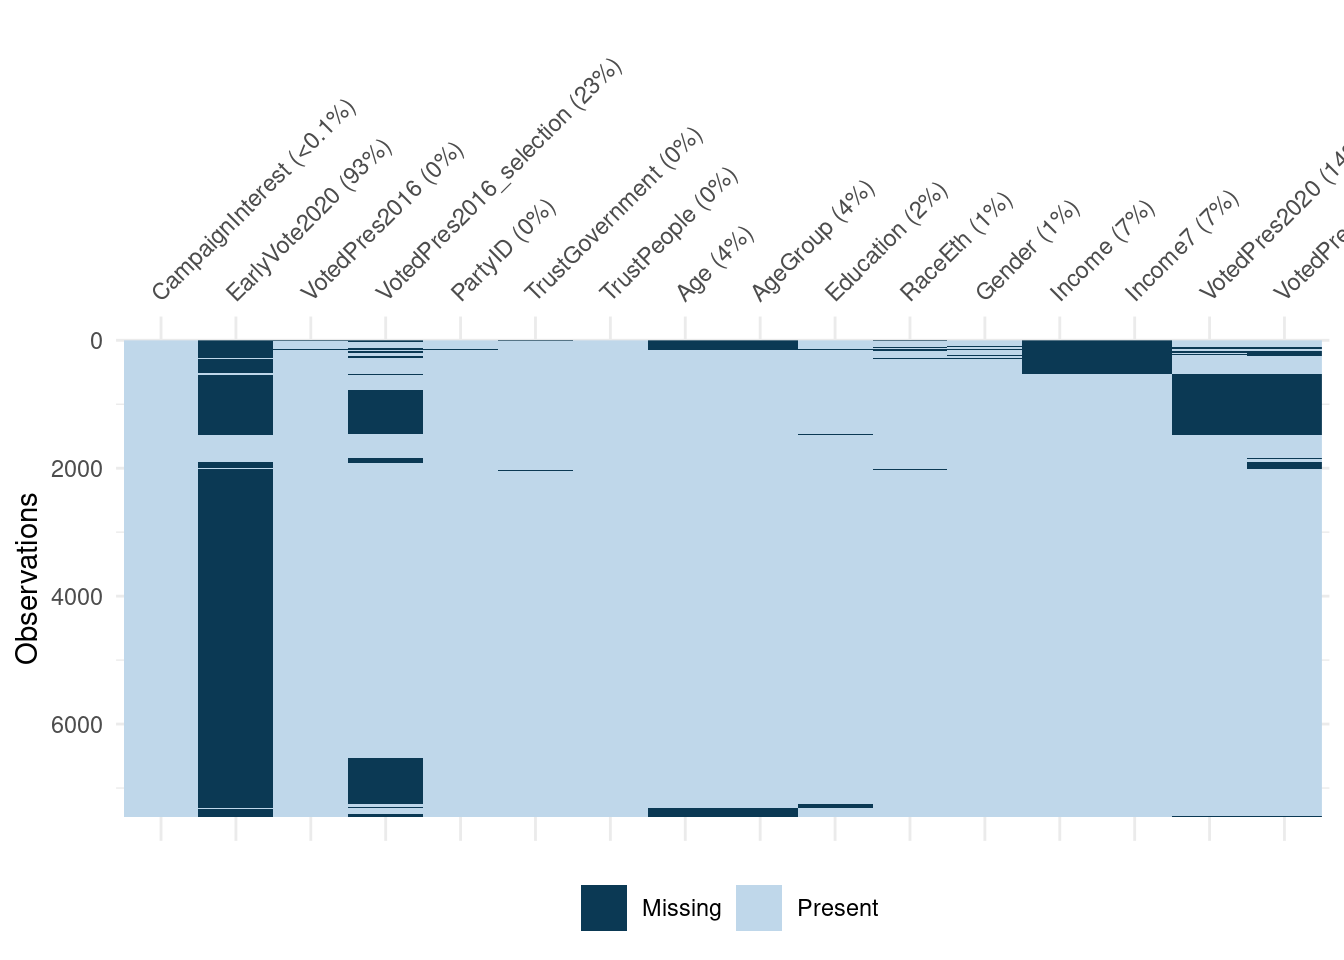
\includegraphics{bookdown_files/figure-latex/missing-anes-vismiss-1} \caption{Visual depiction of missing data in the ANES 2020 data}\label{fig:missing-anes-vismiss}
\end{figure}

From this visualization, we can start to get a picture of what questions may be related to each other in terms of missing data. Even if we did not have the informative variable names, we could be able to deduce that \texttt{VotedPres2020}, \texttt{VotedPres2020\_selection}, and \texttt{EarlyVote2020} are likely related since their missing data patterns are similar.

Additionally, we can also look at \texttt{VotedPres2016\_selection} and see that there is a lot of missing data in that variable. Most likely this is due to a skip pattern, and we can look at further graphics to see how it might be related to other variables. The \{naniar\} package has multiple visualization functions that can help dive deeper such as the \texttt{gg\_miss\_fct()} function which looks at missing data for all variables by levels of another variable.

\begin{Shaded}
\begin{Highlighting}[]
\NormalTok{anes\_2020\_derived }\SpecialCharTok{\%\textgreater{}\%}
  \FunctionTok{gg\_miss\_fct}\NormalTok{(VotedPres2016) }\SpecialCharTok{+}
  \FunctionTok{scale\_fill\_gradientn}\NormalTok{(}
    \AttributeTok{guide =} \StringTok{"colorbar"}\NormalTok{,}
    \AttributeTok{name =} \StringTok{"\% Miss"}\NormalTok{,}
    \AttributeTok{colors =}\NormalTok{ book\_colors[}\FunctionTok{c}\NormalTok{(}\DecValTok{3}\NormalTok{, }\DecValTok{2}\NormalTok{, }\DecValTok{1}\NormalTok{)]}
\NormalTok{  ) }\SpecialCharTok{+}
  \FunctionTok{ylab}\NormalTok{(}\StringTok{"Variable"}\NormalTok{) }\SpecialCharTok{+}
  \FunctionTok{xlab}\NormalTok{(}\StringTok{"Voted for President in 2016"}\NormalTok{)}
\end{Highlighting}
\end{Shaded}

\begin{verbatim}
## Scale for fill is already present.
## Adding another scale for fill, which will replace the existing scale.
\end{verbatim}

\begin{figure}
\includegraphics{bookdown_files/figure-latex/unnamed-chunk-265-1} \caption{Missingness in variables for each level of `VotedPres2016` in the ANES 2020 data}\label{fig:unnamed-chunk-265}
\end{figure}

In this case, we can see that if they did not vote for president in 2016 or did not answer that question, then they were not asked about who they voted for in 2016 (the percentage of missing data if 100\%). Additionally, we can see with this graphic, that there is more missing data across all questions if they did not provide an answer to \texttt{VotedPres2016}.

There are other graphics that work well with numeric data. For example, in the RECS 2020 data we can plot two continuous variables and the missing data associated with it to see if there are any patterns to the missingness. To do this, we can use the \texttt{bind\_shadow()} function from the \{naniar\} package. This creates a \textbf{nabular} (combination of ``na'' with ``tabular''), which features the original columns followed by the same number of columns with a specific \texttt{NA} format. These \texttt{NA} columns are indicators of if the value in the original data is missing or not. The example printed below shows how most levels of \texttt{HeatingBehavior} are not missing \texttt{!NA} in the NA variable of \texttt{HeatingBehavior\_NA}, but those missing in \texttt{HeatingBehavior} are also missing in \texttt{HeatingBehavior\_NA}.

\begin{Shaded}
\begin{Highlighting}[]
\NormalTok{recs\_2020\_shadow }\OtherTok{\textless{}{-}}\NormalTok{ recs\_2020 }\SpecialCharTok{\%\textgreater{}\%}
  \FunctionTok{bind\_shadow}\NormalTok{()}

\FunctionTok{ncol}\NormalTok{(recs\_2020)}
\end{Highlighting}
\end{Shaded}

\begin{verbatim}
## [1] 118
\end{verbatim}

\begin{Shaded}
\begin{Highlighting}[]
\FunctionTok{ncol}\NormalTok{(recs\_2020\_shadow)}
\end{Highlighting}
\end{Shaded}

\begin{verbatim}
## [1] 236
\end{verbatim}

\begin{Shaded}
\begin{Highlighting}[]
\NormalTok{recs\_2020\_shadow }\SpecialCharTok{\%\textgreater{}\%}
  \FunctionTok{count}\NormalTok{(HeatingBehavior, HeatingBehavior\_NA)}
\end{Highlighting}
\end{Shaded}

\begin{verbatim}
## # A tibble: 7 x 3
##   HeatingBehavior                               HeatingBehavior_NA     n
##   <fct>                                         <fct>              <int>
## 1 Set one temp and leave it                     !NA                 7806
## 2 Manually adjust at night/no one home          !NA                 4654
## 3 Programmable or smart thermostat automatical~ !NA                 3310
## 4 Turn on or off as needed                      !NA                 1491
## 5 No control                                    !NA                  438
## 6 Other                                         !NA                   46
## 7 <NA>                                          NA                   751
\end{verbatim}

We can then use these new variables to plot the missing data along side the actual data. For example, let's plot a histogram of the total electric bill grouped by those that are missing and not missing by heating behavior.

\begin{Shaded}
\begin{Highlighting}[]
\NormalTok{recs\_2020\_shadow }\SpecialCharTok{\%\textgreater{}\%}
  \FunctionTok{filter}\NormalTok{(TOTALDOL }\SpecialCharTok{\textless{}} \DecValTok{5000}\NormalTok{) }\SpecialCharTok{\%\textgreater{}\%}
  \FunctionTok{ggplot}\NormalTok{(}\FunctionTok{aes}\NormalTok{(}\AttributeTok{x =}\NormalTok{ TOTALDOL, }\AttributeTok{fill =}\NormalTok{ HeatingBehavior\_NA)) }\SpecialCharTok{+}
  \FunctionTok{geom\_histogram}\NormalTok{() }\SpecialCharTok{+}
  \FunctionTok{scale\_fill\_manual}\NormalTok{(}
    \AttributeTok{values =}\NormalTok{ book\_colors[}\FunctionTok{c}\NormalTok{(}\DecValTok{3}\NormalTok{, }\DecValTok{1}\NormalTok{)],}
    \AttributeTok{labels =} \FunctionTok{c}\NormalTok{(}\StringTok{"Present"}\NormalTok{, }\StringTok{"Missing"}\NormalTok{),}
    \AttributeTok{name =} \StringTok{"Heating Behavior"}
\NormalTok{  ) }\SpecialCharTok{+}
  \FunctionTok{theme\_minimal}\NormalTok{() }\SpecialCharTok{+}
  \FunctionTok{xlab}\NormalTok{(}\StringTok{"Total Energy Cost (Truncated at $5000)"}\NormalTok{) }\SpecialCharTok{+}
  \FunctionTok{ylab}\NormalTok{(}\StringTok{"Number of Households"}\NormalTok{) }\SpecialCharTok{+}
  \FunctionTok{labs}\NormalTok{(}\AttributeTok{title =} \StringTok{"Histogram of Energy Cost by Heating Behavior Missing Data"}\NormalTok{)}
\end{Highlighting}
\end{Shaded}

\begin{verbatim}
## `stat_bin()` using `bins = 30`. Pick better value with `binwidth`.
\end{verbatim}

\begin{figure}
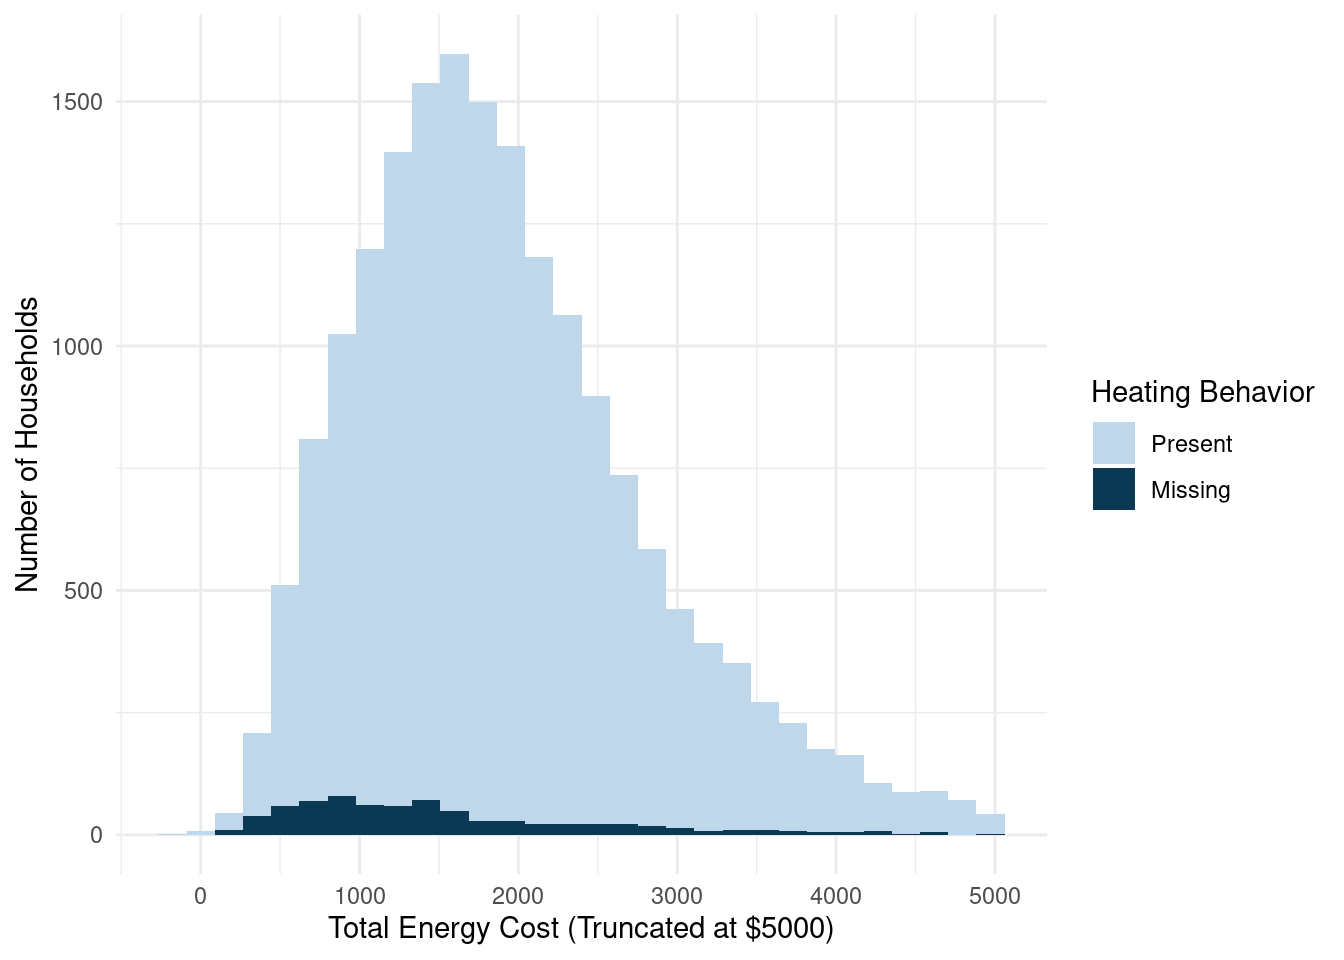
\includegraphics{bookdown_files/figure-latex/missing-recs-hist-1} \caption{Histogram of Energy Cost by Heating Behavior Missing Data}\label{fig:missing-recs-hist}
\end{figure}

This plot indicates that respondents who did not provide a response for the heating behavior question may have a different distribution of total energy cost compared to respondents who did provide a response. This view of the raw data and missingness could indicate some bias in the data. Researchers take these different bias aspects into account when calculating weights and we need to make sure that the weights are incorporated when analyzing the data.

There are many other visualizations that can be helpful in reviewing the data, and we recommend reviewing the \{naniar\} documentation for more information \citep{naniar}.

\hypertarget{analysis-with-missing-data}{%
\section{Analysis with missing data}\label{analysis-with-missing-data}}

Once we understand the types of missingness, we can begin the analysis of the data. Different missingness types may be handled in different ways. In most publicly available datasets, researchers will have already calculated weights and imputed missing values if deemed necessary. Those interested in learning more about how to calculate weights and impute data for different missing data mechanisms, we recommended \citet{Kim2021} and \citet{Valliant2018weights}.

Even with weights and imputation, missing data will still most likely exist in the data and need to be accounted for in analysis. This section provides an overview on how to recode missing data in R, and how to account for skip patterns in analysis.

\hypertarget{recoding-missing-data}{%
\subsection{Recoding missing data}\label{recoding-missing-data}}

Even within a variable, there can be different reasons for missing data. In publicly released data negative values are often present to provide different meaning for values. For example, in the ANES 2020 data they have the following negative values to represent different types of missing data:
* -9: Refused
* -8: Don't Know
* -7: No post-election data, deleted due to incomplete interview
* -6: No post-election interview
* -5: Interview breakoff (sufficient partial IW)
* -4: Technical error
* -3: Restricted
* -2: Other missing reason (question specific)
* -1: Inapplicable

When we created the derived variables for use in this book, we coded all negative values as \texttt{NA} and proceeded to analyze the data. For most cases this is an appropriate approach as long as you filter the data appropriately to account for skip patterns (see next section). However, the \{nanair\} package does have the option to code special missing values. For example, if we wanted to have two \texttt{NA} values, one that indicated the question was missing by design (e.g., due to skip patterns) and one for the other missing categories we can use the \texttt{nabular} format to incorporate these with the \texttt{recode\_shadow()} function.

\begin{Shaded}
\begin{Highlighting}[]
\NormalTok{anes\_2020\_shadow }\OtherTok{\textless{}{-}}\NormalTok{ anes\_2020 }\SpecialCharTok{\%\textgreater{}\%}
  \FunctionTok{select}\NormalTok{(}\FunctionTok{starts\_with}\NormalTok{(}\StringTok{"V2"}\NormalTok{)) }\SpecialCharTok{\%\textgreater{}\%}
  \FunctionTok{mutate}\NormalTok{(}\FunctionTok{across}\NormalTok{(}\FunctionTok{everything}\NormalTok{(), }\SpecialCharTok{\textasciitilde{}} \FunctionTok{case\_when}\NormalTok{(}
\NormalTok{    .x }\SpecialCharTok{\textless{}} \SpecialCharTok{{-}}\DecValTok{1} \SpecialCharTok{\textasciitilde{}} \ConstantTok{NA}\NormalTok{,}
    \ConstantTok{TRUE} \SpecialCharTok{\textasciitilde{}}\NormalTok{ .x}
\NormalTok{  ))) }\SpecialCharTok{\%\textgreater{}\%}
  \FunctionTok{bind\_shadow}\NormalTok{() }\SpecialCharTok{\%\textgreater{}\%}
  \FunctionTok{recode\_shadow}\NormalTok{(}\AttributeTok{V201103 =} \FunctionTok{.where}\NormalTok{(V201103 }\SpecialCharTok{==} \SpecialCharTok{{-}}\DecValTok{1} \SpecialCharTok{\textasciitilde{}} \StringTok{"skip"}\NormalTok{))}

\NormalTok{anes\_2020\_shadow }\SpecialCharTok{\%\textgreater{}\%}
  \FunctionTok{count}\NormalTok{(V201103, V201103\_NA)}
\end{Highlighting}
\end{Shaded}

\begin{verbatim}
## # A tibble: 5 x 3
##   V201103                 V201103_NA     n
##   <dbl+lbl>               <fct>      <int>
## 1 -1 [-1. Inapplicable]   NA_skip     1643
## 2  1 [1. Hillary Clinton] !NA         2911
## 3  2 [2. Donald Trump]    !NA         2466
## 4  5 [5. Other {SPECIFY}] !NA          390
## 5 NA                      NA            43
\end{verbatim}

However it is important to note that at the time of publication, there is no easy way to implement \texttt{recode\_shadow()} to multiple variables at once (e.g., we cannot use the tidyverse feature of \texttt{across()}). The example code above only implements this for a single variable, so this would have to be done to all variables of interest manually or in a loop.

\hypertarget{accounting-for-skip-patterns}{%
\subsection{Accounting for skip patterns}\label{accounting-for-skip-patterns}}

When questions are skipped by design in a survey, it is meaningful that the data is later missing. For example the RECS survey asks people how they control the heat in their home in the winter (\texttt{HeatingBehavior}). This is only among those who have heat in their home (\texttt{SpaceHeatingUsed}). If no there is no heating equipment used, the value of \texttt{HeatingBehavior} is missing. One has several choices when analyzing this data which include 1) only including those with a valid value of \texttt{HeatingBehavior} and specifying the universe as those with heat or 2) including those who do not have heat. It is important to specify what population an analysis generalizes to.

Here is example code where we only include those with a valid value of \texttt{HeatingBehavior} (choice 1). Note that we use the design object (\texttt{recs\_des}) then filter to those that are not missing on \texttt{HeatingBehavior}.

\begin{Shaded}
\begin{Highlighting}[]
\NormalTok{heat\_cntl\_1 }\OtherTok{\textless{}{-}}\NormalTok{ recs\_des }\SpecialCharTok{\%\textgreater{}\%}
  \FunctionTok{filter}\NormalTok{(}\SpecialCharTok{!}\FunctionTok{is.na}\NormalTok{(HeatingBehavior)) }\SpecialCharTok{\%\textgreater{}\%}
  \FunctionTok{group\_by}\NormalTok{(HeatingBehavior) }\SpecialCharTok{\%\textgreater{}\%}
  \FunctionTok{summarize}\NormalTok{(}
    \AttributeTok{p =} \FunctionTok{survey\_prop}\NormalTok{()}
\NormalTok{  )}

\NormalTok{heat\_cntl\_1}
\end{Highlighting}
\end{Shaded}

\begin{verbatim}
## # A tibble: 6 x 3
##   HeatingBehavior                                              p    p_se
##   <fct>                                                    <dbl>   <dbl>
## 1 Set one temp and leave it                              0.430   4.69e-3
## 2 Manually adjust at night/no one home                   0.264   4.54e-3
## 3 Programmable or smart thermostat automatically adjust~ 0.168   3.12e-3
## 4 Turn on or off as needed                               0.102   2.89e-3
## 5 No control                                             0.0333  1.70e-3
## 6 Other                                                  0.00208 3.59e-4
\end{verbatim}

Here is example code where we include those that do not have heat (choice 2). To help understand what we are looking at we have included the output to show both variables \texttt{SpaceHeatingUsed} and \texttt{HeatingBehavior}.

\begin{Shaded}
\begin{Highlighting}[]
\NormalTok{heat\_cntl\_2 }\OtherTok{\textless{}{-}}\NormalTok{ recs\_des }\SpecialCharTok{\%\textgreater{}\%}
  \FunctionTok{group\_by}\NormalTok{(}\FunctionTok{interact}\NormalTok{(SpaceHeatingUsed, HeatingBehavior)) }\SpecialCharTok{\%\textgreater{}\%}
  \FunctionTok{summarize}\NormalTok{(}
    \AttributeTok{p =} \FunctionTok{survey\_prop}\NormalTok{()}
\NormalTok{  )}

\NormalTok{heat\_cntl\_2}
\end{Highlighting}
\end{Shaded}

\begin{verbatim}
## # A tibble: 7 x 4
##   SpaceHeatingUsed HeatingBehavior                             p    p_se
##   <lgl>            <fct>                                   <dbl>   <dbl>
## 1 FALSE            <NA>                                  0.0469  2.07e-3
## 2 TRUE             Set one temp and leave it             0.410   4.60e-3
## 3 TRUE             Manually adjust at night/no one home  0.251   4.36e-3
## 4 TRUE             Programmable or smart thermostat aut~ 0.160   2.95e-3
## 5 TRUE             Turn on or off as needed              0.0976  2.79e-3
## 6 TRUE             No control                            0.0317  1.62e-3
## 7 TRUE             Other                                 0.00198 3.41e-4
\end{verbatim}

If we ran the first analysis, we would say that 16.8\% \textbf{of households with heat} use a programmable or smart thermostat for the heating of their home. While if we used the results from the second analysis, we could say that 16\% of households use a programmable or smart thermostat for the heating of their home. The distinction of the two statements is bolded for emphasis. Skip patterns often change the universe that we are talking about and need to be carefully examined.

Filtering to the correct universe is important when handling these types of missing data. The \texttt{nabular} we created above can also help with this. If we have \texttt{NA\_skip} values in the shadow, we can make sure that we filter out all of these values and only include relevant missing. To do this with survey data we could first create the \texttt{nabular}, then create the design object on that data, and then use the shadow variables to assist with filtering the data. Let's use the \texttt{nabular} we created above for ANES 2020 (\texttt{anes\_2020\_shadow}) to create the design object.

\begin{Shaded}
\begin{Highlighting}[]
\NormalTok{anes\_adjwgt\_shadow }\OtherTok{\textless{}{-}}\NormalTok{ anes\_2020\_shadow }\SpecialCharTok{\%\textgreater{}\%}
  \FunctionTok{mutate}\NormalTok{(}\AttributeTok{V200010b =}\NormalTok{ V200010b }\SpecialCharTok{/} \FunctionTok{sum}\NormalTok{(V200010b) }\SpecialCharTok{*}\NormalTok{ targetpop)}

\NormalTok{anes\_des\_shadow }\OtherTok{\textless{}{-}}\NormalTok{ anes\_adjwgt\_shadow }\SpecialCharTok{\%\textgreater{}\%}
  \FunctionTok{as\_survey\_design}\NormalTok{(}
    \AttributeTok{weights =}\NormalTok{ V200010b,}
    \AttributeTok{strata =}\NormalTok{ V200010d,}
    \AttributeTok{ids =}\NormalTok{ V200010c,}
    \AttributeTok{nest =} \ConstantTok{TRUE}
\NormalTok{  )}
\end{Highlighting}
\end{Shaded}

Then we can use this design object to look at the percent of the population that voted for each candidate in 2016 (\texttt{V201103}). First, let's look at the percentages without removing any cases:

\begin{Shaded}
\begin{Highlighting}[]
\NormalTok{pres16\_select1 }\OtherTok{\textless{}{-}}\NormalTok{ anes\_des\_shadow }\SpecialCharTok{\%\textgreater{}\%}
  \FunctionTok{group\_by}\NormalTok{(V201103) }\SpecialCharTok{\%\textgreater{}\%}
  \FunctionTok{summarize}\NormalTok{(}
    \AttributeTok{All\_Missing =} \FunctionTok{survey\_prop}\NormalTok{()}
\NormalTok{  )}

\NormalTok{pres16\_select1}
\end{Highlighting}
\end{Shaded}

\begin{verbatim}
## # A tibble: 5 x 3
##   V201103                 All_Missing All_Missing_se
##   <dbl+lbl>                     <dbl>          <dbl>
## 1 -1 [-1. Inapplicable]       0.324          0.00933
## 2  1 [1. Hillary Clinton]     0.330          0.00728
## 3  2 [2. Donald Trump]        0.299          0.00728
## 4  5 [5. Other {SPECIFY}]     0.0409         0.00230
## 5 NA                          0.00627        0.00121
\end{verbatim}

Next, we will look at the percentages removing only those that were missing due to skip patterns (i.e., they did not receive this question).

\begin{Shaded}
\begin{Highlighting}[]
\NormalTok{pres16\_select2 }\OtherTok{\textless{}{-}}\NormalTok{ anes\_des\_shadow }\SpecialCharTok{\%\textgreater{}\%}
  \FunctionTok{filter}\NormalTok{(V201103\_NA }\SpecialCharTok{!=} \StringTok{"NA\_skip"}\NormalTok{) }\SpecialCharTok{\%\textgreater{}\%}
  \FunctionTok{group\_by}\NormalTok{(V201103) }\SpecialCharTok{\%\textgreater{}\%}
  \FunctionTok{summarize}\NormalTok{(}
    \AttributeTok{No\_Skip\_Missing =} \FunctionTok{survey\_prop}\NormalTok{()}
\NormalTok{  )}

\NormalTok{pres16\_select2}
\end{Highlighting}
\end{Shaded}

\begin{verbatim}
## # A tibble: 4 x 3
##   V201103                 No_Skip_Missing No_Skip_Missing_se
##   <dbl+lbl>                         <dbl>              <dbl>
## 1  1 [1. Hillary Clinton]         0.488              0.00870
## 2  2 [2. Donald Trump]            0.443              0.00856
## 3  5 [5. Other {SPECIFY}]         0.0606             0.00330
## 4 NA                              0.00928            0.00178
\end{verbatim}

Finally, we will look at the percentages removing all missing values both due to skip patterns and due to those who refused to answer the question.

\begin{Shaded}
\begin{Highlighting}[]
\NormalTok{pres16\_select3 }\OtherTok{\textless{}{-}}\NormalTok{ anes\_des\_shadow }\SpecialCharTok{\%\textgreater{}\%}
  \FunctionTok{filter}\NormalTok{(V201103\_NA }\SpecialCharTok{==} \StringTok{"!NA"}\NormalTok{) }\SpecialCharTok{\%\textgreater{}\%}
  \FunctionTok{group\_by}\NormalTok{(V201103) }\SpecialCharTok{\%\textgreater{}\%}
  \FunctionTok{summarize}\NormalTok{(}
    \AttributeTok{No\_Missing =} \FunctionTok{survey\_prop}\NormalTok{()}
\NormalTok{  )}

\NormalTok{pres16\_select3}
\end{Highlighting}
\end{Shaded}

\begin{verbatim}
## # A tibble: 3 x 3
##   V201103                No_Missing No_Missing_se
##   <dbl+lbl>                   <dbl>         <dbl>
## 1 1 [1. Hillary Clinton]     0.492        0.00875
## 2 2 [2. Donald Trump]        0.447        0.00861
## 3 5 [5. Other {SPECIFY}]     0.0611       0.00332
\end{verbatim}



\begin{longtable}{lrrrrrr}
\caption{\label{tab:missing-anes-shadow-tab}Percentage of Votes by Candidate for Different Missing Data Inclusions}\\
\toprule
 & \multicolumn{2}{c}{Including All Missing Data} & \multicolumn{2}{c}{Removing Skip Patterns Only} & \multicolumn{2}{c}{Removing All Missing Data} \\ 
\cmidrule(lr){2-3} \cmidrule(lr){4-5} \cmidrule(lr){6-7}
Candidate & \% & s.e. (\%) & \% & s.e. (\%) & \% & s.e. (\%) \\ 
\midrule
Did not Vote for President in 2016 & $32.4\%$ & $0.9\%$ & NA & NA & NA & NA \\ 
Hillary Clinton & $33.0\%$ & $0.7\%$ & $48.8\%$ & $0.9\%$ & $49.2\%$ & $0.9\%$ \\ 
Donald Trump & $29.9\%$ & $0.7\%$ & $44.3\%$ & $0.9\%$ & $44.7\%$ & $0.9\%$ \\ 
Other Candidate & $4.1\%$ & $0.2\%$ & $6.1\%$ & $0.3\%$ & $6.1\%$ & $0.3\%$ \\ 
Missing & $0.6\%$ & $0.1\%$ & $0.9\%$ & $0.2\%$ & NA & NA \\ 
\bottomrule
\end{longtable}

As Table \ref{tab:missing-anes-shadow-tab} shows, the results can vary greatly depending on which type of missing data that are removed. If we remove only the skip patterns the margin between the Clinton and Trump is 4.5 percentage points, but if we include all data even including those that did not vote in 2016, the margin is 3.1 percentage points. How we handle the different types of missing values is important for interpretation of the data.

\hypertarget{c12-pitfalls}{%
\chapter{Common pitfalls}\label{c12-pitfalls}}

\hypertarget{part-vignettes}{%
\part{Vignettes}\label{part-vignettes}}

\hypertarget{c13-ncvs-vignette}{%
\chapter{National Crime Victimization Survey Vignette}\label{c13-ncvs-vignette}}

\begin{prereqbox}{Prerequisites}

For this chapter, load the following packages:

\begin{Shaded}
\begin{Highlighting}[]
\FunctionTok{library}\NormalTok{(tidyverse)}
\FunctionTok{library}\NormalTok{(survey)}
\FunctionTok{library}\NormalTok{(srvyr)}
\FunctionTok{library}\NormalTok{(srvyrexploR)}
\FunctionTok{library}\NormalTok{(gt)}
\end{Highlighting}
\end{Shaded}

We will use data from the United States National Crime Victimization Survey (NCVS). Here is the code to read in the three datasets from the \{srvyrexploR\} package:

\begin{Shaded}
\begin{Highlighting}[]
\FunctionTok{data}\NormalTok{(ncvs\_2021\_incident)}
\FunctionTok{data}\NormalTok{(ncvs\_2021\_household)}
\FunctionTok{data}\NormalTok{(ncvs\_2021\_person)}
\end{Highlighting}
\end{Shaded}

\end{prereqbox}

\hypertarget{introduction-10}{%
\section{Introduction}\label{introduction-10}}

The NCVS is a household survey sponsored by the Bureau of Justice Statistics (BJS), which collects data on criminal victimization, including characteristics of the crimes, offenders, and victims. Crime types include both household and personal crimes, as well as violent and non-violent crimes. The target population of this survey is all people in the United States age 12 and older living in housing units and noninstitutional group quarters.

The NCVS has been ongoing since 1992. An earlier survey, the National Crime Survey, was run from 1972 to 1991 \citep{ncvs_tech_2016}. The survey is administered using a rotating panel. When an address enters the sample, the residents of that address are interviewed every six months for a total of seven interviews. If the initial residents move away from the address during the period, the new residents are included in the survey, as people are not followed when they move.

NCVS data is publicly available and distributed by Inter-university Consortium for Political and Social Research (ICPSR)\footnote{\url{https://www.icpsr.umich.edu/web/ICPSR/series/95}}, with data going back to 1992. The vignette in this book will include data from 2021 \citep{ncvs_data_2021}. The NCVS data structure is complicated, and the User's Guide contains examples for analysis in SAS, SUDAAN, SPSS, and Stata, but not R \citep{ncvs_user_guide}. This vignette will adapt those examples for R.

\hypertarget{data-structure}{%
\section{Data Structure}\label{data-structure}}

The data from ICPSR is distributed with five files, each having its unique identifier indicated:

\begin{itemize}
\tightlist
\item
  Address Record - \texttt{YEARQ}, \texttt{IDHH}
\item
  Household Record - \texttt{YEARQ}, \texttt{IDHH}
\item
  Person Record - \texttt{YEARQ}, \texttt{IDHH}, \texttt{IDPER}
\item
  Incident Record - \texttt{YEARQ}, \texttt{IDHH}, \texttt{IDPER}
\item
  2021 Collection Year Incident - \texttt{YEARQ}, \texttt{IDHH}, \texttt{IDPER}
\end{itemize}

We will focus on the household, person, and incident files. From these files, we selected a subset of columns for examples to use in this vignette. We have included data in the \{srvyexploR\} package with a subset of columns, but you can download the complete files at ICPSR\footnote{\url{https://www.icpsr.umich.edu/web/NACJD/studies/38429}}.

\hypertarget{survey-notation}{%
\section{Survey Notation}\label{survey-notation}}

The NCVS User Guide \citep{ncvs_user_guide} uses the following notation:

\begin{itemize}
\tightlist
\item
  \(i\) represents NCVS households, identified on the household-level file with the household identification number \texttt{IDHH}.
\item
  \(j\) represents NCVS individual respondents within households \(i\), identified on the person-level file with the person identification number \texttt{IDPER}.
\item
  \(k\) represents reporting periods (i.e., \texttt{YEARQ}) for households \(i\) and individual respondent \(j\).
\item
  \(l\) represents victimization records for respondent \(j\) in household \(i\) and reporting period \(k\). Each record on the NCVS incident-level file is associated with a victimization record \(l\).
\item
  \(D\) represents one or more domain characteristics of interest in the calculation of NCVS estimates. For victimization totals and proportions, domains can be defined on the basis of crime types (e.g., violent crimes, property crimes), characteristics of victims (e.g., age, sex, household income), or characteristics of the victimizations (e.g., victimizations reported to police, victimizations committed with a weapon present). Domains could also be a combination of all of these types of characteristics. For example, in the calculation of victimization rates, domains are defined on the basis of the characteristics of the victims.
\item
  \(A_a\) represents the level \(a\) of covariate \(A\). Covariate \(A\) is defined in the calculation of victimization proportions and represents the characteristic for which the analyst wants to obtain the distribution of victimizations in domain \(D\).
\item
  \(C\) represents the personal or property crime for which we want to obtain a victimization rate.
\end{itemize}

In this vignette, we will discuss four estimates:

\begin{enumerate}
\def\labelenumi{\arabic{enumi}.}
\tightlist
\item
  \emph{Victimization totals} estimate the number of criminal victimizations with a given characteristic. As demonstrated below, these can be calculated from any of the data files. The estimated victimization total, \(\hat{t}_D\) for domain \(D\) is estimated as
\end{enumerate}

\[ \hat{t}_D = \sum_{ijkl \in D} v_{ijkl}\]

where \(v_{ijkl}\) is the series-adjusted victimization weight for household \(i\), respondent \(j\), reporting period \(k\), and victimization \(l\), that is \texttt{WGTVICCY}.

\begin{enumerate}
\def\labelenumi{\arabic{enumi}.}
\setcounter{enumi}{1}
\tightlist
\item
  \emph{Victimization proportions} estimate characteristics among victimizations or victims. Victimization proportions are calculated using the incident data file. The estimated victimization proportion for domain \(D\) across level \(a\) of covariate \(A\), \(\hat{p}_{A_a,D}\) is
\end{enumerate}

\[ \hat{p}_{A_a,D} =\frac{\sum_{ijkl \in A_a, D} v_{ijkl}}{\sum_{ijkl \in D} v_{ijkl}}.\]
The numerator is the number of incidents with a particular characteristic in a domain, and the denominator is the number of incidents in a domain.

\begin{enumerate}
\def\labelenumi{\arabic{enumi}.}
\setcounter{enumi}{2}
\tightlist
\item
  \emph{Victimization rates} are estimates of the number of victimizations per 1,000 persons or households in the population\footnote{BJS publishes victimization rates per 1,000, which are also presented in these examples}. Victimization rates are calculated using the household or person-level data files. The estimated victimization rate for crime \(C\) in domain \(D\) is
\end{enumerate}

\[\hat{VR}_{C,D}= \frac{\sum_{ijkl \in C,D} v_{ijkl}}{\sum_{ijk \in D} w_{ijk}}\times 1000\]
where \(w_{ijk}\) is the person weight (\texttt{WGTPERCY}) or household weight (\texttt{WGTHHCY}) for personal and household crimes, respectively. The numerator is the number of incidents in a domain, and the denominator is the number of persons or households in a domain. Notice that the weights in the numerator and denominator are different - this is important, and in the syntax and examples below, we will discuss how to make an estimate that involves two weights.

\begin{enumerate}
\def\labelenumi{\arabic{enumi}.}
\setcounter{enumi}{3}
\tightlist
\item
  \emph{Prevalence rates} are estimates of the percentage of the population (persons or households) who are victims of a crime. These are estimated using the household or person-level data files. The estimated prevalence rate for crime \(C\) in domain \(D\) is
\end{enumerate}

\[ \hat{PR}_{C, D}= \frac{\sum_{ijk \in {C,D}} I_{ij}w_{ijk}}{\sum_{ijk \in D} w_{ijk}} \times 100\]

where \(I_{ij}\) is an indicator that a person or household in domain \(D\) was a victim of crime \(C\) at any time in the year. The numerator is the number of victims in domain \(D\) for crime \(C\), and the denominator is the number of people or households in the population.

\hypertarget{data-file-preparation}{%
\section{Data File Preparation}\label{data-file-preparation}}

Some work is necessary to prepare the files before analysis. The design variables indicating pseudostratum (\texttt{V2117}) and half-sample code (\texttt{V2118}) are only included on the household file, so they must be added to the person and incident files for any analysis.

For victimization rates, we need to know the victimization status for both victims and non-victims. Therefore, the incident file must be summarized and merged onto the household or person files for household-level and person-level crimes, respectively. We begin this vignette by discussing how to create these incident summary files. This is following Section 2.2 of the NCVS User's Guide \citep{ncvs_user_guide}.

\hypertarget{preparing-files-for-estimation-of-victimization-rates}{%
\subsection{Preparing Files for Estimation of Victimization Rates}\label{preparing-files-for-estimation-of-victimization-rates}}

Each record on the incident file represents one victimization, which is not the same as one incident. Some victimizations have several instances that make it difficult for the victim to differentiate the details of these incidents, labeled as ``series crimes''. Appendix A of the User's Guide indicates how to calculate the series weight in other statistical languages.

Here, we adapt that code for R. Essentially, if a victimization is a series crime, its series weight is top-coded at 10 based on the number of actual victimizations, that is that even if the crime repeatedly occurred more than 10 times, it is counted as 10 times to reduce the influence of extreme outliers. If an incident is a series crime, but the number of occurrences is unknown, the series weight is set to 6. A description of the variables used to create indicators of series and the associated weights is included in Table \ref{tab:cb-incident}.

\begin{longtable}[]{@{}
  >{\centering\arraybackslash}p{(\columnwidth - 6\tabcolsep) * \real{0.1905}}
  >{\centering\arraybackslash}p{(\columnwidth - 6\tabcolsep) * \real{0.3333}}
  >{\centering\arraybackslash}p{(\columnwidth - 6\tabcolsep) * \real{0.1429}}
  >{\centering\arraybackslash}p{(\columnwidth - 6\tabcolsep) * \real{0.3333}}@{}}
\caption{\label{tab:cb-incident} Codebook for incident variables - related to series weight}\tabularnewline
\toprule\noalign{}
\begin{minipage}[b]{\linewidth}\centering
\end{minipage} & \begin{minipage}[b]{\linewidth}\centering
Description
\end{minipage} & \begin{minipage}[b]{\linewidth}\centering
Value
\end{minipage} & \begin{minipage}[b]{\linewidth}\centering
Label
\end{minipage} \\
\midrule\noalign{}
\endfirsthead
\toprule\noalign{}
\begin{minipage}[b]{\linewidth}\centering
\end{minipage} & \begin{minipage}[b]{\linewidth}\centering
Description
\end{minipage} & \begin{minipage}[b]{\linewidth}\centering
Value
\end{minipage} & \begin{minipage}[b]{\linewidth}\centering
Label
\end{minipage} \\
\midrule\noalign{}
\endhead
\bottomrule\noalign{}
\endlastfoot
V4016 & How many times incident occur last 6 mos & 1-996 & Number of times \\
& & 997 & Don't know \\
V4017 & How many incidents & 1 & 1-5 incidents (not a ``series'') \\
& & 2 & 6 or more incidents \\
& & 8 & Residue (invalid data) \\
V4018 & Incidents similar in detail & 1 & Similar \\
& & 2 & Different (not in a ``series'') \\
& & 8 & Residue (invalid data) \\
V4019 & Enough detail to distinguish incidents & 1 & Yes (not a ``series'') \\
& & 2 & No (is a ``series'') \\
& & 8 & Residue (invalid data) \\
WGTVICCY & Adjusted victimization weight & & Numeric \\
\end{longtable}

We want to create four variables to indicate if an incident is a series crime. First, we create a variable called series using \texttt{V4017}, \texttt{V4018}, and \texttt{V4019} where an incident is considered a series crime if there are 6 or more incidents (\texttt{V4107}), the incidents are similar in detail (\texttt{V4018}), or there is not enough detail to distinguish the incidents (\texttt{V4019}). Next, we top-code the number of incidents (\texttt{V4016}) by creating a variable \texttt{n10v4016} which is set to 10 if \texttt{V4016\ \textgreater{}\ 10}. Finally, we create the series weight using our new top-coded variable and the existing weight.

\begin{Shaded}
\begin{Highlighting}[]
\NormalTok{inc\_series }\OtherTok{\textless{}{-}}\NormalTok{ ncvs\_2021\_incident }\SpecialCharTok{\%\textgreater{}\%}
  \FunctionTok{mutate}\NormalTok{(}
    \AttributeTok{series =} \FunctionTok{case\_when}\NormalTok{(}
\NormalTok{      V4017 }\SpecialCharTok{\%in\%} \FunctionTok{c}\NormalTok{(}\DecValTok{1}\NormalTok{, }\DecValTok{8}\NormalTok{) }\SpecialCharTok{\textasciitilde{}} \DecValTok{1}\NormalTok{,}
\NormalTok{      V4018 }\SpecialCharTok{\%in\%} \FunctionTok{c}\NormalTok{(}\DecValTok{2}\NormalTok{, }\DecValTok{8}\NormalTok{) }\SpecialCharTok{\textasciitilde{}} \DecValTok{1}\NormalTok{,}
\NormalTok{      V4019 }\SpecialCharTok{\%in\%} \FunctionTok{c}\NormalTok{(}\DecValTok{1}\NormalTok{, }\DecValTok{8}\NormalTok{) }\SpecialCharTok{\textasciitilde{}} \DecValTok{1}\NormalTok{,}
      \ConstantTok{TRUE} \SpecialCharTok{\textasciitilde{}} \DecValTok{2}
\NormalTok{    ),}
    \AttributeTok{n10v4016 =} \FunctionTok{case\_when}\NormalTok{(}
\NormalTok{      V4016 }\SpecialCharTok{\%in\%} \FunctionTok{c}\NormalTok{(}\DecValTok{997}\NormalTok{, }\DecValTok{998}\NormalTok{) }\SpecialCharTok{\textasciitilde{}} \ConstantTok{NA\_real\_}\NormalTok{,}
\NormalTok{      V4016 }\SpecialCharTok{\textgreater{}} \DecValTok{10} \SpecialCharTok{\textasciitilde{}} \DecValTok{10}\NormalTok{,}
      \ConstantTok{TRUE} \SpecialCharTok{\textasciitilde{}}\NormalTok{ V4016}
\NormalTok{    ),}
    \AttributeTok{serieswgt =} \FunctionTok{case\_when}\NormalTok{(}
\NormalTok{      series }\SpecialCharTok{==} \DecValTok{2} \SpecialCharTok{\&} \FunctionTok{is.na}\NormalTok{(n10v4016) }\SpecialCharTok{\textasciitilde{}} \DecValTok{6}\NormalTok{,}
\NormalTok{      series }\SpecialCharTok{==} \DecValTok{2} \SpecialCharTok{\textasciitilde{}}\NormalTok{ n10v4016,}
      \ConstantTok{TRUE} \SpecialCharTok{\textasciitilde{}} \DecValTok{1}
\NormalTok{    ),}
    \AttributeTok{NEWWGT =}\NormalTok{ WGTVICCY }\SpecialCharTok{*}\NormalTok{ serieswgt}
\NormalTok{  )}
\end{Highlighting}
\end{Shaded}

The next step in preparing the files for estimation is to create indicators on the victimization file for characteristics of interest. Almost all BJS publications limit the analysis to records where the victimization occurred in the United States, where \texttt{V4022} is not equal to 1, and we will do this for all estimates as well. A brief codebook of variables for this task is located in Table \ref{tab:cb-crimetype}

\begin{longtable}[]{@{}cccc@{}}
\caption{\label{tab:cb-crimetype} Codebook for incident variables - crime type indicators and characteristics}\tabularnewline
\toprule\noalign{}
Variable & Description & Value & Label \\
\midrule\noalign{}
\endfirsthead
\toprule\noalign{}
Variable & Description & Value & Label \\
\midrule\noalign{}
\endhead
\bottomrule\noalign{}
\endlastfoot
V4022 & In what city/town/village & 1 & Outside U.S. \\
& & 2 & Not inside a city/town/village \\
& & 3 & Same city/town/village as present residence \\
& & 4 & Different city/town/village as present residence \\
& & 5 & Don't know \\
& & 6 & Don't know if 2, 4, or 5 \\
V4049 & Did offender have weapon & 1 & Yes \\
& & 2 & No \\
& & 3 & Don't know \\
V4050 & What was weapon & 1 & At least one good entry \\
& & 3 & Indicates ``Yes-Type Weapon-NA'' \\
& & 7 & Indicates ``Gun Type Unknown'' \\
& & 8 & No good entry \\
V4051 & Hand gun & 0 & No \\
& & 1 & Yes \\
V4052 & Other gun & 0 & No \\
& & 1 & Yes \\
V4053 & Knife & 0 & No \\
& & 1 & Yes \\
V4399 & Reported to police & 1 & Yes \\
& & 2 & No \\
& & 3 & Don't know \\
V4529 & Type of crime code & 01 & Completed rape \\
& & 02 & Attempted rape \\
& & 03 & Sexual attack with serious assault \\
& & 04 & Sexual attack with minor assault \\
& & 05 & Completed robbery with injury from serious assault \\
& & 06 & Completed robbery with injury from minor assault \\
& & 07 & Completed robbery without injury from minor assault \\
& & 08 & Attempted robbery with injury from serious assault \\
& & 09 & Attempted robbery with injury from minor assault \\
& & 10 & Attempted robbery without injury \\
& & 11 & Completed aggravated assault with injury \\
& & 12 & Attempted aggravated assault with weapon \\
& & 13 & Threatened assault with weapon \\
& & 14 & Simple assault completed with injury \\
& & 15 & Sexual assault without injury \\
& & 16 & Unwanted sexual contact without force \\
& & 17 & Assault without weapon without injury \\
& & 18 & Verbal threat of rape \\
& & 19 & Verbal threat of sexual assault \\
& & 20 & Verbal threat of assault \\
& & 21 & Completed purse snatching \\
& & 22 & Attempted purse snatching \\
& & 23 & Pocket picking (completed only) \\
& & 31 & Completed burglary, forcible entry \\
& & 32 & Completed burglary, unlawful entry without force \\
& & 33 & Attempted forcible entry \\
& & 40 & Completed motor vehicle theft \\
& & 41 & Attempted motor vehicle theft \\
& & 54 & Completed theft less than \$10 \\
& & 55 & Completed theft \$10 to \$49 \\
& & 56 & Completed theft \$50 to \$249 \\
& & 57 & Completed theft \$250 or greater \\
& & 58 & Completed theft value NA \\
& & 59 & Attempted theft \\
\end{longtable}

Using these variables, we will create the following indicators:

\begin{enumerate}
\def\labelenumi{\arabic{enumi}.}
\tightlist
\item
  Property crime

  \begin{itemize}
  \tightlist
  \item
    \texttt{V4529} \textgreater= 31
  \item
    Variable: \texttt{Property}
  \end{itemize}
\item
  Violent crime

  \begin{itemize}
  \tightlist
  \item
    \texttt{V4529} \textless= 20
  \item
    Variable: \texttt{Violent}
  \end{itemize}
\item
  Property crime reported to the police

  \begin{itemize}
  \tightlist
  \item
    \texttt{V4529} \textgreater= 31 and \texttt{V4399}=1
  \item
    Variable: \texttt{Property\_ReportPolice}
  \end{itemize}
\item
  Violent crime reported to the police

  \begin{itemize}
  \tightlist
  \item
    \texttt{V4529} \textless{} 31 and \texttt{V4399}=1
  \item
    Variable: \texttt{Violent\_ReportPolice}
  \end{itemize}
\item
  Aggravated assault without a weapon

  \begin{itemize}
  \tightlist
  \item
    \texttt{V4529} in 11:12 and \texttt{V4049}=2
  \item
    Variable: \texttt{AAST\_NoWeap}
  \end{itemize}
\item
  Aggravated assault with a firearm

  \begin{itemize}
  \tightlist
  \item
    \texttt{V4529} in 11:12 and \texttt{V4049}=1 and (\texttt{V4051}=1 or \texttt{V4052}=1 or \texttt{V4050}=7)
  \item
    Variable: \texttt{AAST\_Firearm}
  \end{itemize}
\item
  Aggravated assault with a knife or sharp object

  \begin{itemize}
  \tightlist
  \item
    \texttt{V4529} in 11:12 and \texttt{V4049}=1 and (\texttt{V4053}=1 or \texttt{V4054}=1)
  \item
    Variable: \texttt{AAST\_Knife}
  \end{itemize}
\item
  Aggravated assault with another type of weapon

  \begin{itemize}
  \tightlist
  \item
    \texttt{V4529} in 11:12 and \texttt{V4049}=1 and \texttt{V4050}=1 and not firearm or knife
  \item
    Variable: \texttt{AAST\_Other}
  \end{itemize}
\end{enumerate}

\begin{Shaded}
\begin{Highlighting}[]
\NormalTok{inc\_ind }\OtherTok{\textless{}{-}}\NormalTok{ inc\_series }\SpecialCharTok{\%\textgreater{}\%}
  \FunctionTok{filter}\NormalTok{(V4022 }\SpecialCharTok{!=} \DecValTok{1}\NormalTok{) }\SpecialCharTok{\%\textgreater{}\%}
  \FunctionTok{mutate}\NormalTok{(}
    \AttributeTok{WeapCat =} \FunctionTok{case\_when}\NormalTok{(}
      \FunctionTok{is.na}\NormalTok{(V4049) }\SpecialCharTok{\textasciitilde{}} \ConstantTok{NA\_character\_}\NormalTok{,}
\NormalTok{      V4049 }\SpecialCharTok{==} \DecValTok{2} \SpecialCharTok{\textasciitilde{}} \StringTok{"NoWeap"}\NormalTok{,}
\NormalTok{      V4049 }\SpecialCharTok{==} \DecValTok{3} \SpecialCharTok{\textasciitilde{}} \StringTok{"UnkWeapUse"}\NormalTok{,}
\NormalTok{      V4050 }\SpecialCharTok{==} \DecValTok{3} \SpecialCharTok{\textasciitilde{}} \StringTok{"Other"}\NormalTok{,}
\NormalTok{      V4051 }\SpecialCharTok{==} \DecValTok{1} \SpecialCharTok{|}\NormalTok{ V4052 }\SpecialCharTok{==} \DecValTok{1} \SpecialCharTok{|}\NormalTok{ V4050 }\SpecialCharTok{==} \DecValTok{7} \SpecialCharTok{\textasciitilde{}} \StringTok{"Firearm"}\NormalTok{,}
\NormalTok{      V4053 }\SpecialCharTok{==} \DecValTok{1} \SpecialCharTok{|}\NormalTok{ V4054 }\SpecialCharTok{==} \DecValTok{1} \SpecialCharTok{\textasciitilde{}} \StringTok{"Knife"}\NormalTok{,}
      \ConstantTok{TRUE} \SpecialCharTok{\textasciitilde{}} \StringTok{"Other"}
\NormalTok{    ),}
    \AttributeTok{V4529\_num =} \FunctionTok{parse\_number}\NormalTok{(}\FunctionTok{as.character}\NormalTok{(V4529)),}
    \AttributeTok{ReportPolice =}\NormalTok{ V4399 }\SpecialCharTok{==} \DecValTok{1}\NormalTok{,}
    \AttributeTok{Property =}\NormalTok{ V4529\_num }\SpecialCharTok{\textgreater{}=} \DecValTok{31}\NormalTok{,}
    \AttributeTok{Violent =}\NormalTok{ V4529\_num }\SpecialCharTok{\textless{}=} \DecValTok{20}\NormalTok{,}
    \AttributeTok{Property\_ReportPolice =}\NormalTok{ Property }\SpecialCharTok{\&}\NormalTok{ ReportPolice,}
    \AttributeTok{Violent\_ReportPolice =}\NormalTok{ Violent }\SpecialCharTok{\&}\NormalTok{ ReportPolice,}
    \AttributeTok{AAST =}\NormalTok{ V4529\_num }\SpecialCharTok{\%in\%} \DecValTok{11}\SpecialCharTok{:}\DecValTok{13}\NormalTok{,}
    \AttributeTok{AAST\_NoWeap =}\NormalTok{ AAST }\SpecialCharTok{\&}\NormalTok{ WeapCat }\SpecialCharTok{==} \StringTok{"NoWeap"}\NormalTok{,}
    \AttributeTok{AAST\_Firearm =}\NormalTok{ AAST }\SpecialCharTok{\&}\NormalTok{ WeapCat }\SpecialCharTok{==} \StringTok{"Firearm"}\NormalTok{,}
    \AttributeTok{AAST\_Knife =}\NormalTok{ AAST }\SpecialCharTok{\&}\NormalTok{ WeapCat }\SpecialCharTok{==} \StringTok{"Knife"}\NormalTok{,}
    \AttributeTok{AAST\_Other =}\NormalTok{ AAST }\SpecialCharTok{\&}\NormalTok{ WeapCat }\SpecialCharTok{==} \StringTok{"Other"}
\NormalTok{  )}
\end{Highlighting}
\end{Shaded}

This is a good point to pause to look at the output of crosswalks between an original variable and a derived one to check that the logic was programmed correctly and that everything ends up in the expected category.

\begin{Shaded}
\begin{Highlighting}[]
\NormalTok{inc\_series }\SpecialCharTok{\%\textgreater{}\%} \FunctionTok{count}\NormalTok{(V4022)}
\end{Highlighting}
\end{Shaded}

\begin{verbatim}
## # A tibble: 6 x 2
##   V4022     n
##   <fct> <int>
## 1 1        34
## 2 2        65
## 3 3      7697
## 4 4      1143
## 5 5        39
## 6 8         4
\end{verbatim}

\begin{Shaded}
\begin{Highlighting}[]
\NormalTok{inc\_ind }\SpecialCharTok{\%\textgreater{}\%} \FunctionTok{count}\NormalTok{(V4022)}
\end{Highlighting}
\end{Shaded}

\begin{verbatim}
## # A tibble: 5 x 2
##   V4022     n
##   <fct> <int>
## 1 2        65
## 2 3      7697
## 3 4      1143
## 4 5        39
## 5 8         4
\end{verbatim}

\begin{Shaded}
\begin{Highlighting}[]
\NormalTok{inc\_ind }\SpecialCharTok{\%\textgreater{}\%}
  \FunctionTok{count}\NormalTok{(WeapCat, V4049, V4050, V4051, V4052, V4052, V4053, V4054)}
\end{Highlighting}
\end{Shaded}

\begin{verbatim}
## # A tibble: 13 x 8
##    WeapCat    V4049 V4050 V4051 V4052 V4053 V4054     n
##    <chr>      <fct> <fct> <fct> <fct> <fct> <fct> <int>
##  1 Firearm    1     1     0     1     0     0        15
##  2 Firearm    1     1     0     1     1     1         1
##  3 Firearm    1     1     1     0     0     0       125
##  4 Firearm    1     1     1     0     1     0         2
##  5 Firearm    1     1     1     1     0     0         3
##  6 Firearm    1     7     0     0     0     0         3
##  7 Knife      1     1     0     0     0     1        14
##  8 Knife      1     1     0     0     1     0        71
##  9 NoWeap     2     <NA>  <NA>  <NA>  <NA>  <NA>   1794
## 10 Other      1     1     0     0     0     0       147
## 11 Other      1     3     0     0     0     0        26
## 12 UnkWeapUse 3     <NA>  <NA>  <NA>  <NA>  <NA>    519
## 13 <NA>       <NA>  <NA>  <NA>  <NA>  <NA>  <NA>   6228
\end{verbatim}

\begin{Shaded}
\begin{Highlighting}[]
\NormalTok{inc\_ind }\SpecialCharTok{\%\textgreater{}\%}
  \FunctionTok{count}\NormalTok{(V4529, Property, Violent, AAST) }\SpecialCharTok{\%\textgreater{}\%}
  \FunctionTok{print}\NormalTok{(}\AttributeTok{n =} \DecValTok{40}\NormalTok{)}
\end{Highlighting}
\end{Shaded}

\begin{verbatim}
## # A tibble: 34 x 5
##    V4529 Property Violent AAST      n
##    <fct> <lgl>    <lgl>   <lgl> <int>
##  1 1     FALSE    TRUE    FALSE    45
##  2 2     FALSE    TRUE    FALSE    20
##  3 3     FALSE    TRUE    FALSE    11
##  4 4     FALSE    TRUE    FALSE     3
##  5 5     FALSE    TRUE    FALSE    24
##  6 6     FALSE    TRUE    FALSE    26
##  7 7     FALSE    TRUE    FALSE    59
##  8 8     FALSE    TRUE    FALSE     5
##  9 9     FALSE    TRUE    FALSE     7
## 10 10    FALSE    TRUE    FALSE    57
## 11 11    FALSE    TRUE    TRUE     97
## 12 12    FALSE    TRUE    TRUE     91
## 13 13    FALSE    TRUE    TRUE    163
## 14 14    FALSE    TRUE    FALSE   165
## 15 15    FALSE    TRUE    FALSE    24
## 16 16    FALSE    TRUE    FALSE    12
## 17 17    FALSE    TRUE    FALSE   357
## 18 18    FALSE    TRUE    FALSE    14
## 19 19    FALSE    TRUE    FALSE     3
## 20 20    FALSE    TRUE    FALSE   607
## 21 21    FALSE    FALSE   FALSE     2
## 22 22    FALSE    FALSE   FALSE     2
## 23 23    FALSE    FALSE   FALSE    19
## 24 31    TRUE     FALSE   FALSE   248
## 25 32    TRUE     FALSE   FALSE   634
## 26 33    TRUE     FALSE   FALSE   188
## 27 40    TRUE     FALSE   FALSE   256
## 28 41    TRUE     FALSE   FALSE    97
## 29 54    TRUE     FALSE   FALSE   407
## 30 55    TRUE     FALSE   FALSE  1006
## 31 56    TRUE     FALSE   FALSE  1686
## 32 57    TRUE     FALSE   FALSE  1420
## 33 58    TRUE     FALSE   FALSE   798
## 34 59    TRUE     FALSE   FALSE   395
\end{verbatim}

\begin{Shaded}
\begin{Highlighting}[]
\NormalTok{inc\_ind }\SpecialCharTok{\%\textgreater{}\%} \FunctionTok{count}\NormalTok{(ReportPolice, V4399)}
\end{Highlighting}
\end{Shaded}

\begin{verbatim}
## # A tibble: 4 x 3
##   ReportPolice V4399     n
##   <lgl>        <fct> <int>
## 1 FALSE        2      5670
## 2 FALSE        3       103
## 3 FALSE        8        12
## 4 TRUE         1      3163
\end{verbatim}

\begin{Shaded}
\begin{Highlighting}[]
\NormalTok{inc\_ind }\SpecialCharTok{\%\textgreater{}\%}
  \FunctionTok{count}\NormalTok{(}
\NormalTok{    AAST,}
\NormalTok{    WeapCat,}
\NormalTok{    AAST\_NoWeap,}
\NormalTok{    AAST\_Firearm,}
\NormalTok{    AAST\_Knife,}
\NormalTok{    AAST\_Other}
\NormalTok{  )}
\end{Highlighting}
\end{Shaded}

\begin{verbatim}
## # A tibble: 11 x 7
##    AAST  WeapCat    AAST_NoWeap AAST_Firearm AAST_Knife AAST_Other     n
##    <lgl> <chr>      <lgl>       <lgl>        <lgl>      <lgl>      <int>
##  1 FALSE Firearm    FALSE       FALSE        FALSE      FALSE         34
##  2 FALSE Knife      FALSE       FALSE        FALSE      FALSE         23
##  3 FALSE NoWeap     FALSE       FALSE        FALSE      FALSE       1769
##  4 FALSE Other      FALSE       FALSE        FALSE      FALSE         27
##  5 FALSE UnkWeapUse FALSE       FALSE        FALSE      FALSE        516
##  6 FALSE <NA>       FALSE       FALSE        FALSE      FALSE       6228
##  7 TRUE  Firearm    FALSE       TRUE         FALSE      FALSE        115
##  8 TRUE  Knife      FALSE       FALSE        TRUE       FALSE         62
##  9 TRUE  NoWeap     TRUE        FALSE        FALSE      FALSE         25
## 10 TRUE  Other      FALSE       FALSE        FALSE      TRUE         146
## 11 TRUE  UnkWeapUse FALSE       FALSE        FALSE      FALSE          3
\end{verbatim}

After creating indicators of victimization types and characteristics, the file is summarized, and crimes are summed across persons or households by \texttt{YEARQ.} Property crimes (i.e., crimes committed against households, such as household burglary or motor vehicle theft) are summed across households, and personal crimes (i.e., crimes committed against an individual, such as assault, robbery, and personal theft) are summed across persons. The indicators are summed using the \texttt{serieswgt}, and the variable \texttt{WGTVICCY} needs to be retained for later analysis.

\begin{Shaded}
\begin{Highlighting}[]
\NormalTok{inc\_hh\_sums }\OtherTok{\textless{}{-}}
\NormalTok{  inc\_ind }\SpecialCharTok{\%\textgreater{}\%}
  \FunctionTok{filter}\NormalTok{(V4529\_num }\SpecialCharTok{\textgreater{}} \DecValTok{23}\NormalTok{) }\SpecialCharTok{\%\textgreater{}\%} \CommentTok{\# restrict to household crimes}
  \FunctionTok{group\_by}\NormalTok{(YEARQ, IDHH) }\SpecialCharTok{\%\textgreater{}\%}
  \FunctionTok{summarize}\NormalTok{(}
    \AttributeTok{WGTVICCY =}\NormalTok{ WGTVICCY[}\DecValTok{1}\NormalTok{],}
    \FunctionTok{across}\NormalTok{(}\FunctionTok{starts\_with}\NormalTok{(}\StringTok{"Property"}\NormalTok{),}
      \SpecialCharTok{\textasciitilde{}} \FunctionTok{sum}\NormalTok{(. }\SpecialCharTok{*}\NormalTok{ serieswgt),}
      \AttributeTok{.names =} \StringTok{"\{.col\}"}
\NormalTok{    ),}
    \AttributeTok{.groups =} \StringTok{"drop"}
\NormalTok{  )}

\NormalTok{inc\_pers\_sums }\OtherTok{\textless{}{-}}
\NormalTok{  inc\_ind }\SpecialCharTok{\%\textgreater{}\%}
  \FunctionTok{filter}\NormalTok{(V4529\_num }\SpecialCharTok{\textless{}=} \DecValTok{23}\NormalTok{) }\SpecialCharTok{\%\textgreater{}\%} \CommentTok{\# restrict to person crimes}
  \FunctionTok{group\_by}\NormalTok{(YEARQ, IDHH, IDPER) }\SpecialCharTok{\%\textgreater{}\%}
  \FunctionTok{summarize}\NormalTok{(}
    \AttributeTok{WGTVICCY =}\NormalTok{ WGTVICCY[}\DecValTok{1}\NormalTok{],}
    \FunctionTok{across}\NormalTok{(}\FunctionTok{c}\NormalTok{(}\FunctionTok{starts\_with}\NormalTok{(}\StringTok{"Violent"}\NormalTok{), }\FunctionTok{starts\_with}\NormalTok{(}\StringTok{"AAST"}\NormalTok{)),}
      \SpecialCharTok{\textasciitilde{}} \FunctionTok{sum}\NormalTok{(. }\SpecialCharTok{*}\NormalTok{ serieswgt),}
      \AttributeTok{.names =} \StringTok{"\{.col\}"}
\NormalTok{    ),}
    \AttributeTok{.groups =} \StringTok{"drop"}
\NormalTok{  )}
\end{Highlighting}
\end{Shaded}

Now, we merge the victimization summary files into the appropriate files. For any record on the household or person file that is not on the victimization file, the victimization counts are set to 0 after merging. In this step, we will also create the victimization adjustment factor. See 2.2.4 in the User's Guide for details of why this adjustment is created (\citet{ncvs_user_guide}). It is calculated as follows:

\[ A_{ijk}=\frac{v_{ijk}}{w_{ijk}}\]

where \(w_{ijk}\) is the person weight (\texttt{WGTPERCY}) for personal crimes or the household weight (\texttt{WGTHHCY}) for household crimes, and \(v_{ijk}\) is the victimization weight (\texttt{WGTVICCY}) for household \(i\), respondent \(j\), in reporting period \(k\). The adjustment factor is set to 0 if no incidents are reported.

\begin{Shaded}
\begin{Highlighting}[]
\CommentTok{\# Set up a list of 0s for each crime type/characteristic to replace NA\textquotesingle{}s}
\NormalTok{hh\_z\_list }\OtherTok{\textless{}{-}} \FunctionTok{rep}\NormalTok{(}\DecValTok{0}\NormalTok{, }\FunctionTok{ncol}\NormalTok{(inc\_hh\_sums) }\SpecialCharTok{{-}} \DecValTok{3}\NormalTok{) }\SpecialCharTok{\%\textgreater{}\%}
  \FunctionTok{as.list}\NormalTok{() }\SpecialCharTok{\%\textgreater{}\%}
  \FunctionTok{setNames}\NormalTok{(}\FunctionTok{names}\NormalTok{(inc\_hh\_sums)[}\SpecialCharTok{{-}}\NormalTok{(}\DecValTok{1}\SpecialCharTok{:}\DecValTok{3}\NormalTok{)])}
\NormalTok{pers\_z\_list }\OtherTok{\textless{}{-}} \FunctionTok{rep}\NormalTok{(}\DecValTok{0}\NormalTok{, }\FunctionTok{ncol}\NormalTok{(inc\_pers\_sums) }\SpecialCharTok{{-}} \DecValTok{4}\NormalTok{) }\SpecialCharTok{\%\textgreater{}\%}
  \FunctionTok{as.list}\NormalTok{() }\SpecialCharTok{\%\textgreater{}\%}
  \FunctionTok{setNames}\NormalTok{(}\FunctionTok{names}\NormalTok{(inc\_pers\_sums)[}\SpecialCharTok{{-}}\NormalTok{(}\DecValTok{1}\SpecialCharTok{:}\DecValTok{4}\NormalTok{)])}

\NormalTok{hh\_vsum }\OtherTok{\textless{}{-}}\NormalTok{ ncvs\_2021\_household }\SpecialCharTok{\%\textgreater{}\%}
  \FunctionTok{full\_join}\NormalTok{(inc\_hh\_sums, }\AttributeTok{by =} \FunctionTok{c}\NormalTok{(}\StringTok{"YEARQ"}\NormalTok{, }\StringTok{"IDHH"}\NormalTok{)) }\SpecialCharTok{\%\textgreater{}\%}
  \FunctionTok{replace\_na}\NormalTok{(hh\_z\_list) }\SpecialCharTok{\%\textgreater{}\%}
  \FunctionTok{mutate}\NormalTok{(}\AttributeTok{ADJINC\_WT =} \FunctionTok{if\_else}\NormalTok{(}\FunctionTok{is.na}\NormalTok{(WGTVICCY), }\DecValTok{0}\NormalTok{, WGTVICCY }\SpecialCharTok{/}\NormalTok{ WGTHHCY))}

\NormalTok{pers\_vsum }\OtherTok{\textless{}{-}}\NormalTok{ ncvs\_2021\_person }\SpecialCharTok{\%\textgreater{}\%}
  \FunctionTok{full\_join}\NormalTok{(inc\_pers\_sums, }\AttributeTok{by =} \FunctionTok{c}\NormalTok{(}\StringTok{"YEARQ"}\NormalTok{, }\StringTok{"IDHH"}\NormalTok{, }\StringTok{"IDPER"}\NormalTok{)) }\SpecialCharTok{\%\textgreater{}\%}
  \FunctionTok{replace\_na}\NormalTok{(pers\_z\_list) }\SpecialCharTok{\%\textgreater{}\%}
  \FunctionTok{mutate}\NormalTok{(}\AttributeTok{ADJINC\_WT =} \FunctionTok{if\_else}\NormalTok{(}\FunctionTok{is.na}\NormalTok{(WGTVICCY), }\DecValTok{0}\NormalTok{, WGTVICCY }\SpecialCharTok{/}\NormalTok{ WGTPERCY))}
\end{Highlighting}
\end{Shaded}

\hypertarget{derived-demographic-variables}{%
\subsection{Derived Demographic Variables}\label{derived-demographic-variables}}

A final step in file preparation for the household and person files is creating any derived variables on the household and person files, such as income categories or age categories, for subgroup analysis. We can do this step before or after merging the victimization counts.

\hypertarget{household-variables}{%
\subsubsection{Household Variables}\label{household-variables}}

For the household file, we create categories for tenure (rental status), urbanicity, income, place size, and region. A codebook of the household variables are located in Table \ref{tab:cb-hh}.

\begin{longtable}[]{@{}llll@{}}
\caption{\label{tab:cb-hh} Codebook for household variables}\tabularnewline
\toprule\noalign{}
Variable & Description & Value & Label \\
\midrule\noalign{}
\endfirsthead
\toprule\noalign{}
Variable & Description & Value & Label \\
\midrule\noalign{}
\endhead
\bottomrule\noalign{}
\endlastfoot
V2015 & Tenure & 1 & Owned or being bought \\
& & 2 & Rented for cash \\
& & 3 & No cash rent \\
SC214A & Household Income & 01 & Less than \$5,000 \\
& & 02 & \$5,000 to \$7,499 \\
& & 03 & \$7,500 to \$9,999 \\
& & 04 & \$10,000 to \$12,499 \\
& & 05 & \$12,500 to \$14,999 \\
& & 06 & \$15,000 to \$17,499 \\
& & 07 & \$17,500 to \$19,999 \\
& & 08 & \$20,000 to \$24,999 \\
& & 09 & \$25,000 to \$29,999 \\
& & 10 & \$30,000 to \$34,999 \\
& & 11 & \$35,000 to \$39,999 \\
& & 12 & \$40,000 to \$49,999 \\
& & 13 & \$50,000 to \$74,999 \\
& & 15 & \$75,000 to \$99,999 \\
& & 16 & \$100,000-\$149,999 \\
& & 17 & \$150,000-\$199,999 \\
& & 18 & \$200,000 or more \\
V2126B & Place Size Code & 00 & Not in a place \\
& & 13 & Under 10,000 \\
& & 16 & 10,000-49,999 \\
& & 17 & 50,000-99,999 \\
& & 18 & 100,000-249,999 \\
& & 19 & 250,000-499,999 \\
& & 20 & 500,000-999,999 \\
& & 21 & 1,000,000-2,499,999 \\
& & 22 & 2,500,000-4,999,999 \\
& & 23 & 5,000,000 or more \\
V2127B & Region & 1 & Northeast \\
& & 2 & Midwest \\
& & 3 & South \\
& & 4 & West \\
V2143 & Urbanicity & 1 & Urban \\
& & 2 & Suburban \\
& & 3 & Rural \\
\end{longtable}

\begin{Shaded}
\begin{Highlighting}[]
\NormalTok{hh\_vsum\_der }\OtherTok{\textless{}{-}}\NormalTok{ hh\_vsum }\SpecialCharTok{\%\textgreater{}\%}
  \FunctionTok{mutate}\NormalTok{(}
    \AttributeTok{Tenure =} \FunctionTok{factor}\NormalTok{(}
      \FunctionTok{case\_when}\NormalTok{(}
\NormalTok{        V2015 }\SpecialCharTok{==} \DecValTok{1} \SpecialCharTok{\textasciitilde{}} \StringTok{"Owned"}\NormalTok{,}
        \SpecialCharTok{!}\FunctionTok{is.na}\NormalTok{(V2015) }\SpecialCharTok{\textasciitilde{}} \StringTok{"Rented"}
\NormalTok{      ),}
      \AttributeTok{levels =} \FunctionTok{c}\NormalTok{(}\StringTok{"Owned"}\NormalTok{, }\StringTok{"Rented"}\NormalTok{)}
\NormalTok{    ),}
    \AttributeTok{Urbanicity =} \FunctionTok{factor}\NormalTok{(}
      \FunctionTok{case\_when}\NormalTok{(}
\NormalTok{        V2143 }\SpecialCharTok{==} \DecValTok{1} \SpecialCharTok{\textasciitilde{}} \StringTok{"Urban"}\NormalTok{,}
\NormalTok{        V2143 }\SpecialCharTok{==} \DecValTok{2} \SpecialCharTok{\textasciitilde{}} \StringTok{"Suburban"}\NormalTok{,}
\NormalTok{        V2143 }\SpecialCharTok{==} \DecValTok{3} \SpecialCharTok{\textasciitilde{}} \StringTok{"Rural"}
\NormalTok{      ),}
      \AttributeTok{levels =} \FunctionTok{c}\NormalTok{(}\StringTok{"Urban"}\NormalTok{, }\StringTok{"Suburban"}\NormalTok{, }\StringTok{"Rural"}\NormalTok{)}
\NormalTok{    ),}
    \AttributeTok{SC214A\_num =} \FunctionTok{as.numeric}\NormalTok{(}\FunctionTok{as.character}\NormalTok{(SC214A)),}
    \AttributeTok{Income =} \FunctionTok{case\_when}\NormalTok{(}
\NormalTok{      SC214A\_num }\SpecialCharTok{\textless{}=} \DecValTok{8} \SpecialCharTok{\textasciitilde{}} \StringTok{"Less than $25,000"}\NormalTok{,}
\NormalTok{      SC214A\_num }\SpecialCharTok{\textless{}=} \DecValTok{12} \SpecialCharTok{\textasciitilde{}} \StringTok{"$25,000{-}49,999"}\NormalTok{,}
\NormalTok{      SC214A\_num }\SpecialCharTok{\textless{}=} \DecValTok{15} \SpecialCharTok{\textasciitilde{}} \StringTok{"$50,000{-}99,999"}\NormalTok{,}
\NormalTok{      SC214A\_num }\SpecialCharTok{\textless{}=} \DecValTok{17} \SpecialCharTok{\textasciitilde{}} \StringTok{"$100,000{-}199,999"}\NormalTok{,}
\NormalTok{      SC214A\_num }\SpecialCharTok{\textless{}=} \DecValTok{18} \SpecialCharTok{\textasciitilde{}} \StringTok{"$200,000 or more"}
\NormalTok{    ),}
    \AttributeTok{Income =} \FunctionTok{fct\_reorder}\NormalTok{(Income, SC214A\_num, }\AttributeTok{.na\_rm =} \ConstantTok{FALSE}\NormalTok{),}
    \AttributeTok{PlaceSize =} \FunctionTok{case\_match}\NormalTok{(}
      \FunctionTok{as.numeric}\NormalTok{(}\FunctionTok{as.character}\NormalTok{(V2126B)),}
      \DecValTok{0} \SpecialCharTok{\textasciitilde{}} \StringTok{"Not in a place"}\NormalTok{,}
      \DecValTok{13} \SpecialCharTok{\textasciitilde{}} \StringTok{"Under 10,000"}\NormalTok{,}
      \DecValTok{16} \SpecialCharTok{\textasciitilde{}} \StringTok{"10,000{-}49,999"}\NormalTok{,}
      \DecValTok{17} \SpecialCharTok{\textasciitilde{}} \StringTok{"50,000{-}99,999"}\NormalTok{,}
      \DecValTok{18} \SpecialCharTok{\textasciitilde{}} \StringTok{"100,000{-}249,999"}\NormalTok{,}
      \DecValTok{19} \SpecialCharTok{\textasciitilde{}} \StringTok{"250,000{-}499,999"}\NormalTok{,}
      \DecValTok{20} \SpecialCharTok{\textasciitilde{}} \StringTok{"500,000{-}999,999"}\NormalTok{,}
      \FunctionTok{c}\NormalTok{(}\DecValTok{21}\NormalTok{, }\DecValTok{22}\NormalTok{, }\DecValTok{23}\NormalTok{) }\SpecialCharTok{\textasciitilde{}} \StringTok{"1,000,000 or more"}
\NormalTok{    ),}
    \AttributeTok{PlaceSize =} \FunctionTok{fct\_reorder}\NormalTok{(PlaceSize, }\FunctionTok{as.numeric}\NormalTok{(V2126B)),}
    \AttributeTok{Region =} \FunctionTok{case\_match}\NormalTok{(}
      \FunctionTok{as.numeric}\NormalTok{(V2127B),}
      \DecValTok{1} \SpecialCharTok{\textasciitilde{}} \StringTok{"Northeast"}\NormalTok{,}
      \DecValTok{2} \SpecialCharTok{\textasciitilde{}} \StringTok{"Midwest"}\NormalTok{,}
      \DecValTok{3} \SpecialCharTok{\textasciitilde{}} \StringTok{"South"}\NormalTok{,}
      \DecValTok{4} \SpecialCharTok{\textasciitilde{}} \StringTok{"West"}
\NormalTok{    ),}
    \AttributeTok{Region =} \FunctionTok{fct\_reorder}\NormalTok{(Region, }\FunctionTok{as.numeric}\NormalTok{(V2127B))}
\NormalTok{  )}
\end{Highlighting}
\end{Shaded}

As before, we want to check to make sure the recoded variables we create match the existing data as expected.

\begin{Shaded}
\begin{Highlighting}[]
\NormalTok{hh\_vsum\_der }\SpecialCharTok{\%\textgreater{}\%} \FunctionTok{count}\NormalTok{(Tenure, V2015)}
\end{Highlighting}
\end{Shaded}

\begin{verbatim}
## # A tibble: 4 x 3
##   Tenure V2015      n
##   <fct>  <fct>  <int>
## 1 Owned  1     101944
## 2 Rented 2      46269
## 3 Rented 3       1925
## 4 <NA>   <NA>  106322
\end{verbatim}

\begin{Shaded}
\begin{Highlighting}[]
\NormalTok{hh\_vsum\_der }\SpecialCharTok{\%\textgreater{}\%} \FunctionTok{count}\NormalTok{(Urbanicity, V2143)}
\end{Highlighting}
\end{Shaded}

\begin{verbatim}
## # A tibble: 3 x 3
##   Urbanicity V2143      n
##   <fct>      <fct>  <int>
## 1 Urban      1      26878
## 2 Suburban   2     173491
## 3 Rural      3      56091
\end{verbatim}

\begin{Shaded}
\begin{Highlighting}[]
\NormalTok{hh\_vsum\_der }\SpecialCharTok{\%\textgreater{}\%} \FunctionTok{count}\NormalTok{(Income, SC214A)}
\end{Highlighting}
\end{Shaded}

\begin{verbatim}
## # A tibble: 18 x 3
##    Income            SC214A     n
##    <fct>             <fct>  <int>
##  1 Less than $25,000 1       7841
##  2 Less than $25,000 2       2626
##  3 Less than $25,000 3       3949
##  4 Less than $25,000 4       5546
##  5 Less than $25,000 5       5445
##  6 Less than $25,000 6       4821
##  7 Less than $25,000 7       5038
##  8 Less than $25,000 8      11887
##  9 $25,000-49,999    9      11550
## 10 $25,000-49,999    10     13689
## 11 $25,000-49,999    11     13655
## 12 $25,000-49,999    12     23282
## 13 $50,000-99,999    13     44601
## 14 $50,000-99,999    15     33353
## 15 $100,000-199,999  16     34287
## 16 $100,000-199,999  17     15317
## 17 $200,000 or more  18     16892
## 18 <NA>              <NA>    2681
\end{verbatim}

\begin{Shaded}
\begin{Highlighting}[]
\NormalTok{hh\_vsum\_der }\SpecialCharTok{\%\textgreater{}\%} \FunctionTok{count}\NormalTok{(PlaceSize, V2126B)}
\end{Highlighting}
\end{Shaded}

\begin{verbatim}
## # A tibble: 10 x 3
##    PlaceSize         V2126B     n
##    <fct>             <fct>  <int>
##  1 Not in a place    0      69484
##  2 Under 10,000      13     39873
##  3 10,000-49,999     16     53002
##  4 50,000-99,999     17     27205
##  5 100,000-249,999   18     24461
##  6 250,000-499,999   19     13111
##  7 500,000-999,999   20     15194
##  8 1,000,000 or more 21      6167
##  9 1,000,000 or more 22      3857
## 10 1,000,000 or more 23      4106
\end{verbatim}

\begin{Shaded}
\begin{Highlighting}[]
\NormalTok{hh\_vsum\_der }\SpecialCharTok{\%\textgreater{}\%} \FunctionTok{count}\NormalTok{(Region, V2127B)}
\end{Highlighting}
\end{Shaded}

\begin{verbatim}
## # A tibble: 4 x 3
##   Region    V2127B     n
##   <fct>     <fct>  <int>
## 1 Northeast 1      41585
## 2 Midwest   2      74666
## 3 South     3      87783
## 4 West      4      52426
\end{verbatim}

\hypertarget{person-variables}{%
\subsubsection{Person Variables}\label{person-variables}}

For the person file, we create categories for sex, race/Hispanic origin, age categories, and marital status. A codebook of the household variables is located in Table \ref{tab:cb-pers}. We also merge the household demographics to the person file as well as the design variables (\texttt{V2117} and \texttt{V2118}).

\begin{longtable}[]{@{}llll@{}}
\caption{\label{tab:cb-pers} Codebook for person variables}\tabularnewline
\toprule\noalign{}
Variable & Description & Value & Label \\
\midrule\noalign{}
\endfirsthead
\toprule\noalign{}
Variable & Description & Value & Label \\
\midrule\noalign{}
\endhead
\bottomrule\noalign{}
\endlastfoot
V3014 & Age & & 12 through 90 \\
V3015 & Current Marital Status & 1 & Married \\
& & 2 & Widowed \\
& & 3 & Divorced \\
& & 4 & Separated \\
& & 5 & Never married \\
V3018 & Sex & 1 & Male \\
& & 2 & Female \\
V3023A & Race & 01 & White only \\
& & 02 & Black only \\
& & 03 & American Indian, Alaska native only \\
& & 04 & Asian only \\
& & 05 & Hawaiian/Pacific Islander only \\
& & 06 & White-Black \\
& & 07 & White-American Indian \\
& & 08 & White-Asian \\
& & 09 & White-Hawaiian \\
& & 10 & Black-American Indian \\
& & 11 & Black-Asian \\
& & 12 & Black-Hawaiian/Pacific Islander \\
& & 13 & American Indian-Asian \\
& & 14 & Asian-Hawaiian/Pacific Islander \\
& & 15 & White-Black-American Indian \\
& & 16 & White-Black-Asian \\
& & 17 & White-American Indian-Asian \\
& & 18 & White-Asian-Hawaiian \\
& & 19 & 2 or 3 races \\
& & 20 & 4 or 5 races \\
V3024 & Hispanic Origin & 1 & Yes \\
& & 2 & No \\
\end{longtable}

\begin{Shaded}
\begin{Highlighting}[]
\CommentTok{\# Set label for usage later}
\NormalTok{NHOPI }\OtherTok{\textless{}{-}} \StringTok{"Native Hawaiian or Other Pacific Islander"}

\NormalTok{pers\_vsum\_der }\OtherTok{\textless{}{-}}\NormalTok{ pers\_vsum }\SpecialCharTok{\%\textgreater{}\%}
  \FunctionTok{mutate}\NormalTok{(}
    \AttributeTok{Sex =} \FunctionTok{factor}\NormalTok{(}\FunctionTok{case\_when}\NormalTok{(}
\NormalTok{      V3018 }\SpecialCharTok{==} \DecValTok{1} \SpecialCharTok{\textasciitilde{}} \StringTok{"Male"}\NormalTok{,}
\NormalTok{      V3018 }\SpecialCharTok{==} \DecValTok{2} \SpecialCharTok{\textasciitilde{}} \StringTok{"Female"}
\NormalTok{    )),}
    \AttributeTok{RaceHispOrigin =} \FunctionTok{factor}\NormalTok{(}
      \FunctionTok{case\_when}\NormalTok{(}
\NormalTok{        V3024 }\SpecialCharTok{==} \DecValTok{1} \SpecialCharTok{\textasciitilde{}} \StringTok{"Hispanic"}\NormalTok{,}
\NormalTok{        V3023A }\SpecialCharTok{==} \DecValTok{1} \SpecialCharTok{\textasciitilde{}} \StringTok{"White"}\NormalTok{,}
\NormalTok{        V3023A }\SpecialCharTok{==} \DecValTok{2} \SpecialCharTok{\textasciitilde{}} \StringTok{"Black"}\NormalTok{,}
\NormalTok{        V3023A }\SpecialCharTok{==} \DecValTok{4} \SpecialCharTok{\textasciitilde{}} \StringTok{"Asian"}\NormalTok{,}
\NormalTok{        V3023A }\SpecialCharTok{==} \DecValTok{5} \SpecialCharTok{\textasciitilde{}}\NormalTok{ NHOPI,}
        \ConstantTok{TRUE} \SpecialCharTok{\textasciitilde{}} \StringTok{"Other"}
\NormalTok{      ),}
      \AttributeTok{levels =} \FunctionTok{c}\NormalTok{(}
        \StringTok{"White"}\NormalTok{, }\StringTok{"Black"}\NormalTok{, }\StringTok{"Hispanic"}\NormalTok{,}
        \StringTok{"Asian"}\NormalTok{, NHOPI, }\StringTok{"Other"}
\NormalTok{      )}
\NormalTok{    ),}
    \AttributeTok{V3014\_num =} \FunctionTok{as.numeric}\NormalTok{(}\FunctionTok{as.character}\NormalTok{(V3014)),}
    \AttributeTok{AgeGroup =} \FunctionTok{case\_when}\NormalTok{(}
\NormalTok{      V3014\_num }\SpecialCharTok{\textless{}=} \DecValTok{17} \SpecialCharTok{\textasciitilde{}} \StringTok{"12{-}17"}\NormalTok{,}
\NormalTok{      V3014\_num }\SpecialCharTok{\textless{}=} \DecValTok{24} \SpecialCharTok{\textasciitilde{}} \StringTok{"18{-}24"}\NormalTok{,}
\NormalTok{      V3014\_num }\SpecialCharTok{\textless{}=} \DecValTok{34} \SpecialCharTok{\textasciitilde{}} \StringTok{"25{-}34"}\NormalTok{,}
\NormalTok{      V3014\_num }\SpecialCharTok{\textless{}=} \DecValTok{49} \SpecialCharTok{\textasciitilde{}} \StringTok{"35{-}49"}\NormalTok{,}
\NormalTok{      V3014\_num }\SpecialCharTok{\textless{}=} \DecValTok{64} \SpecialCharTok{\textasciitilde{}} \StringTok{"50{-}64"}\NormalTok{,}
\NormalTok{      V3014\_num }\SpecialCharTok{\textless{}=} \DecValTok{90} \SpecialCharTok{\textasciitilde{}} \StringTok{"65 or older"}
\NormalTok{    ),}
    \AttributeTok{AgeGroup =} \FunctionTok{fct\_reorder}\NormalTok{(AgeGroup, V3014\_num),}
    \AttributeTok{MaritalStatus =} \FunctionTok{factor}\NormalTok{(}
      \FunctionTok{case\_when}\NormalTok{(}
\NormalTok{        V3015 }\SpecialCharTok{==} \DecValTok{1} \SpecialCharTok{\textasciitilde{}} \StringTok{"Married"}\NormalTok{,}
\NormalTok{        V3015 }\SpecialCharTok{==} \DecValTok{2} \SpecialCharTok{\textasciitilde{}} \StringTok{"Widowed"}\NormalTok{,}
\NormalTok{        V3015 }\SpecialCharTok{==} \DecValTok{3} \SpecialCharTok{\textasciitilde{}} \StringTok{"Divorced"}\NormalTok{,}
\NormalTok{        V3015 }\SpecialCharTok{==} \DecValTok{4} \SpecialCharTok{\textasciitilde{}} \StringTok{"Separated"}\NormalTok{,}
\NormalTok{        V3015 }\SpecialCharTok{==} \DecValTok{5} \SpecialCharTok{\textasciitilde{}} \StringTok{"Never married"}
\NormalTok{      ),}
      \AttributeTok{levels =} \FunctionTok{c}\NormalTok{(}
        \StringTok{"Never married"}\NormalTok{, }\StringTok{"Married"}\NormalTok{,}
        \StringTok{"Widowed"}\NormalTok{, }\StringTok{"Divorced"}\NormalTok{,}
        \StringTok{"Separated"}
\NormalTok{      )}
\NormalTok{    )}
\NormalTok{  ) }\SpecialCharTok{\%\textgreater{}\%}
  \FunctionTok{left\_join}\NormalTok{(}
\NormalTok{    hh\_vsum\_der }\SpecialCharTok{\%\textgreater{}\%} \FunctionTok{select}\NormalTok{(}
\NormalTok{      YEARQ, IDHH,}
\NormalTok{      V2117, V2118, Tenure}\SpecialCharTok{:}\NormalTok{Region}
\NormalTok{    ),}
    \AttributeTok{by =} \FunctionTok{c}\NormalTok{(}\StringTok{"YEARQ"}\NormalTok{, }\StringTok{"IDHH"}\NormalTok{)}
\NormalTok{  )}
\end{Highlighting}
\end{Shaded}

As before, we want to check to make sure the recoded variables we create match the existing data as expected.

\begin{Shaded}
\begin{Highlighting}[]
\NormalTok{pers\_vsum\_der }\SpecialCharTok{\%\textgreater{}\%} \FunctionTok{count}\NormalTok{(Sex, V3018)}
\end{Highlighting}
\end{Shaded}

\begin{verbatim}
## # A tibble: 2 x 3
##   Sex    V3018      n
##   <fct>  <fct>  <int>
## 1 Female 2     150956
## 2 Male   1     140922
\end{verbatim}

\begin{Shaded}
\begin{Highlighting}[]
\NormalTok{pers\_vsum\_der }\SpecialCharTok{\%\textgreater{}\%} \FunctionTok{count}\NormalTok{(RaceHispOrigin, V3024)}
\end{Highlighting}
\end{Shaded}

\begin{verbatim}
## # A tibble: 11 x 3
##    RaceHispOrigin                            V3024      n
##    <fct>                                     <fct>  <int>
##  1 White                                     2     197292
##  2 White                                     8        883
##  3 Black                                     2      29947
##  4 Black                                     8        120
##  5 Hispanic                                  1      41450
##  6 Asian                                     2      16015
##  7 Asian                                     8         61
##  8 Native Hawaiian or Other Pacific Islander 2        891
##  9 Native Hawaiian or Other Pacific Islander 8          9
## 10 Other                                     2       5161
## 11 Other                                     8         49
\end{verbatim}

\begin{Shaded}
\begin{Highlighting}[]
\NormalTok{pers\_vsum\_der }\SpecialCharTok{\%\textgreater{}\%}
  \FunctionTok{filter}\NormalTok{(RaceHispOrigin }\SpecialCharTok{!=} \StringTok{"Hispanic"} \SpecialCharTok{|}
    \FunctionTok{is.na}\NormalTok{(RaceHispOrigin)) }\SpecialCharTok{\%\textgreater{}\%}
  \FunctionTok{count}\NormalTok{(RaceHispOrigin, V3023A)}
\end{Highlighting}
\end{Shaded}

\begin{verbatim}
## # A tibble: 20 x 3
##    RaceHispOrigin                            V3023A      n
##    <fct>                                     <fct>   <int>
##  1 White                                     1      198175
##  2 Black                                     2       30067
##  3 Asian                                     4       16076
##  4 Native Hawaiian or Other Pacific Islander 5         900
##  5 Other                                     3        1319
##  6 Other                                     6        1217
##  7 Other                                     7        1025
##  8 Other                                     8         837
##  9 Other                                     9         184
## 10 Other                                     10        178
## 11 Other                                     11         87
## 12 Other                                     12         27
## 13 Other                                     13         13
## 14 Other                                     14         53
## 15 Other                                     15        136
## 16 Other                                     16         45
## 17 Other                                     17         11
## 18 Other                                     18         33
## 19 Other                                     19         22
## 20 Other                                     20         23
\end{verbatim}

\begin{Shaded}
\begin{Highlighting}[]
\NormalTok{pers\_vsum\_der }\SpecialCharTok{\%\textgreater{}\%}
  \FunctionTok{group\_by}\NormalTok{(AgeGroup) }\SpecialCharTok{\%\textgreater{}\%}
  \FunctionTok{summarize}\NormalTok{(}
    \AttributeTok{minAge =} \FunctionTok{min}\NormalTok{(V3014),}
    \AttributeTok{maxAge =} \FunctionTok{max}\NormalTok{(V3014),}
    \AttributeTok{.groups =} \StringTok{"drop"}
\NormalTok{  )}
\end{Highlighting}
\end{Shaded}

\begin{verbatim}
## # A tibble: 6 x 3
##   AgeGroup    minAge maxAge
##   <fct>        <dbl>  <dbl>
## 1 12-17           12     17
## 2 18-24           18     24
## 3 25-34           25     34
## 4 35-49           35     49
## 5 50-64           50     64
## 6 65 or older     65     90
\end{verbatim}

\begin{Shaded}
\begin{Highlighting}[]
\NormalTok{pers\_vsum\_der }\SpecialCharTok{\%\textgreater{}\%} \FunctionTok{count}\NormalTok{(MaritalStatus, V3015)}
\end{Highlighting}
\end{Shaded}

\begin{verbatim}
## # A tibble: 6 x 3
##   MaritalStatus V3015      n
##   <fct>         <fct>  <int>
## 1 Never married 5      90425
## 2 Married       1     148131
## 3 Widowed       2      17668
## 4 Divorced      3      28596
## 5 Separated     4       4524
## 6 <NA>          8       2534
\end{verbatim}

We then create tibbles that contain only the variables we need, which makes it easier for analyses.

\begin{Shaded}
\begin{Highlighting}[]
\NormalTok{hh\_vsum\_slim }\OtherTok{\textless{}{-}}\NormalTok{ hh\_vsum\_der }\SpecialCharTok{\%\textgreater{}\%}
  \FunctionTok{select}\NormalTok{(}
\NormalTok{    YEARQ}\SpecialCharTok{:}\NormalTok{V2118,}
\NormalTok{    WGTVICCY}\SpecialCharTok{:}\NormalTok{ADJINC\_WT,}
\NormalTok{    Tenure,}
\NormalTok{    Urbanicity,}
\NormalTok{    Income,}
\NormalTok{    PlaceSize,}
\NormalTok{    Region}
\NormalTok{  )}

\NormalTok{pers\_vsum\_slim }\OtherTok{\textless{}{-}}\NormalTok{ pers\_vsum\_der }\SpecialCharTok{\%\textgreater{}\%}
  \FunctionTok{select}\NormalTok{(YEARQ}\SpecialCharTok{:}\NormalTok{WGTPERCY, WGTVICCY}\SpecialCharTok{:}\NormalTok{ADJINC\_WT, Sex}\SpecialCharTok{:}\NormalTok{Region)}
\end{Highlighting}
\end{Shaded}

To calculate estimates about types of crime, such as what percentage of violent crimes are reported to the police, we must use the incident file. The incident file is not guaranteed to have every pseudostratum and half-sample code, so dummy records are created to append before estimation. Finally, we merge demographic variables onto the incident tibble.

\begin{Shaded}
\begin{Highlighting}[]
\NormalTok{dummy\_records }\OtherTok{\textless{}{-}}\NormalTok{ hh\_vsum\_slim }\SpecialCharTok{\%\textgreater{}\%}
  \FunctionTok{distinct}\NormalTok{(V2117, V2118) }\SpecialCharTok{\%\textgreater{}\%}
  \FunctionTok{mutate}\NormalTok{(}
    \AttributeTok{Dummy =} \DecValTok{1}\NormalTok{,}
    \AttributeTok{WGTVICCY =} \DecValTok{1}\NormalTok{,}
    \AttributeTok{NEWWGT =} \DecValTok{1}
\NormalTok{  )}

\NormalTok{inc\_analysis }\OtherTok{\textless{}{-}}\NormalTok{ inc\_ind }\SpecialCharTok{\%\textgreater{}\%}
  \FunctionTok{mutate}\NormalTok{(}\AttributeTok{Dummy =} \DecValTok{0}\NormalTok{) }\SpecialCharTok{\%\textgreater{}\%}
  \FunctionTok{left\_join}\NormalTok{(}\FunctionTok{select}\NormalTok{(pers\_vsum\_slim, YEARQ, IDHH, IDPER, Sex}\SpecialCharTok{:}\NormalTok{Region),}
    \AttributeTok{by =} \FunctionTok{c}\NormalTok{(}\StringTok{"YEARQ"}\NormalTok{, }\StringTok{"IDHH"}\NormalTok{, }\StringTok{"IDPER"}\NormalTok{)}
\NormalTok{  ) }\SpecialCharTok{\%\textgreater{}\%}
  \FunctionTok{bind\_rows}\NormalTok{(dummy\_records) }\SpecialCharTok{\%\textgreater{}\%}
  \FunctionTok{select}\NormalTok{(}
\NormalTok{    YEARQ}\SpecialCharTok{:}\NormalTok{IDPER,}
\NormalTok{    WGTVICCY,}
\NormalTok{    NEWWGT,}
\NormalTok{    V4529,}
\NormalTok{    WeapCat,}
\NormalTok{    ReportPolice,}
\NormalTok{    Property}\SpecialCharTok{:}\NormalTok{Region}
\NormalTok{  )}
\end{Highlighting}
\end{Shaded}

The tibbles \texttt{hh\_vsum\_slim}, \texttt{pers\_vsum\_slim}, and \texttt{inc\_analysis} can now be used to create design objects and calculate crime rate estimates.

\hypertarget{survey-design-objects}{%
\section{Survey Design Objects}\label{survey-design-objects}}

All the data prep above is necessary to prepare the data for survey analysis. At this point, we can create the design objects and finally begin analysis. We will create three design objects for different types of analysis as they depend on which type of estimate we are creating. For the incident data, the weight of analysis is \texttt{NEWWGT}, which we constructed previously. The household and person-level data use \texttt{WGTHHCY} and \texttt{WGTPERCY}, respectively. For all analyses, \texttt{V2117} is the strata variable, and \texttt{V2118} is the cluster/PSU variable for analysis.

\begin{Shaded}
\begin{Highlighting}[]
\NormalTok{inc\_des }\OtherTok{\textless{}{-}}\NormalTok{ inc\_analysis }\SpecialCharTok{\%\textgreater{}\%}
  \FunctionTok{as\_survey}\NormalTok{(}
    \AttributeTok{weight =}\NormalTok{ NEWWGT,}
    \AttributeTok{strata =}\NormalTok{ V2117,}
    \AttributeTok{ids =}\NormalTok{ V2118,}
    \AttributeTok{nest =} \ConstantTok{TRUE}
\NormalTok{  )}

\NormalTok{hh\_des }\OtherTok{\textless{}{-}}\NormalTok{ hh\_vsum\_slim }\SpecialCharTok{\%\textgreater{}\%}
  \FunctionTok{as\_survey}\NormalTok{(}
    \AttributeTok{weight =}\NormalTok{ WGTHHCY,}
    \AttributeTok{strata =}\NormalTok{ V2117,}
    \AttributeTok{ids =}\NormalTok{ V2118,}
    \AttributeTok{nest =} \ConstantTok{TRUE}
\NormalTok{  )}

\NormalTok{pers\_des }\OtherTok{\textless{}{-}}\NormalTok{ pers\_vsum\_slim }\SpecialCharTok{\%\textgreater{}\%}
  \FunctionTok{as\_survey}\NormalTok{(}
    \AttributeTok{weight =}\NormalTok{ WGTPERCY,}
    \AttributeTok{strata =}\NormalTok{ V2117,}
    \AttributeTok{ids =}\NormalTok{ V2118,}
    \AttributeTok{nest =} \ConstantTok{TRUE}
\NormalTok{  )}
\end{Highlighting}
\end{Shaded}

\hypertarget{calculating-estimates}{%
\section{Calculating Estimates}\label{calculating-estimates}}

Now that we have prepared our data and created the design effects, we can calculate our estimates. As a reminder, those are:

\begin{enumerate}
\def\labelenumi{\arabic{enumi}.}
\item
  \emph{Victimization totals} estimate the number of criminal victimizations with a given characteristic.
\item
  \emph{Victimization proportions} estimate characteristics among victimizations or victims.
\item
  \emph{Victimization rates} are estimates of the number of victimizations per 1,000 persons or households in the population.
\item
  Prevalence rates are estimates of the percentage of the population (persons or households) who are victims of a crime.
\end{enumerate}

\hypertarget{vic-tot}{%
\subsection{Estimation 1: Victimization Totals}\label{vic-tot}}

There are two ways to calculate victimization totals. Using the incident design object (\texttt{inc\_des}) is the most straightforward method, but the person (\texttt{pers\_des}) and household (\texttt{hh\_des}) design objects can be used as well if the adjustment factor (\texttt{ADJINC\_WT}) is incorporated. In the example below, the total number of property and violent victimizations is first calculated using the incident file and then using the household and person design objects. The incident file is smaller, and thus, estimation is faster using that file, but the estimates will be the same as illustrated below:

\begin{Shaded}
\begin{Highlighting}[]
\NormalTok{vt1 }\OtherTok{\textless{}{-}}\NormalTok{ inc\_des }\SpecialCharTok{\%\textgreater{}\%}
  \FunctionTok{summarize}\NormalTok{(}
    \AttributeTok{Property\_Vzn =} \FunctionTok{survey\_total}\NormalTok{(Property, }\AttributeTok{na.rm =} \ConstantTok{TRUE}\NormalTok{),}
    \AttributeTok{Violent\_Vzn =} \FunctionTok{survey\_total}\NormalTok{(Violent, }\AttributeTok{na.rm =} \ConstantTok{TRUE}\NormalTok{)}
\NormalTok{  )}

\NormalTok{vt2a }\OtherTok{\textless{}{-}}\NormalTok{ hh\_des }\SpecialCharTok{\%\textgreater{}\%}
  \FunctionTok{summarize}\NormalTok{(}\AttributeTok{Property\_Vzn =} \FunctionTok{survey\_total}\NormalTok{(Property }\SpecialCharTok{*}\NormalTok{ ADJINC\_WT,}
    \AttributeTok{na.rm =} \ConstantTok{TRUE}
\NormalTok{  ))}

\NormalTok{vt2b }\OtherTok{\textless{}{-}}\NormalTok{ pers\_des }\SpecialCharTok{\%\textgreater{}\%}
  \FunctionTok{summarize}\NormalTok{(}\AttributeTok{Violent\_Vzn =} \FunctionTok{survey\_total}\NormalTok{(Violent }\SpecialCharTok{*}\NormalTok{ ADJINC\_WT,}
    \AttributeTok{na.rm =} \ConstantTok{TRUE}
\NormalTok{  ))}

\NormalTok{vt1}
\end{Highlighting}
\end{Shaded}

\begin{verbatim}
## # A tibble: 1 x 4
##   Property_Vzn Property_Vzn_se Violent_Vzn Violent_Vzn_se
##          <dbl>           <dbl>       <dbl>          <dbl>
## 1    11682056.         263844.    4598306.        198115.
\end{verbatim}

\begin{Shaded}
\begin{Highlighting}[]
\NormalTok{vt2a}
\end{Highlighting}
\end{Shaded}

\begin{verbatim}
## # A tibble: 1 x 2
##   Property_Vzn Property_Vzn_se
##          <dbl>           <dbl>
## 1    11682056.         263844.
\end{verbatim}

\begin{Shaded}
\begin{Highlighting}[]
\NormalTok{vt2b}
\end{Highlighting}
\end{Shaded}

\begin{verbatim}
## # A tibble: 1 x 2
##   Violent_Vzn Violent_Vzn_se
##         <dbl>          <dbl>
## 1    4598306.        198115.
\end{verbatim}

The number of victimizations estimated using the incident file is equivalent to the person and household file method. There are 11,682,056 property incidents and 4,598,306 violent incidents in a six-month period.

\hypertarget{vic-prop}{%
\subsection{Estimation 2: Victimization Proportions}\label{vic-prop}}

Victimization proportions are proportions describing features of a victimization. The key here is that these are questions among victimizations, not among the population. These types of estimates can only be calculated using the incident design object (\texttt{inc\_des}).

For example, we could be interested in the percentage of property victimizations reported to the police as shown in the following code with an estimate, the standard error, and 95\% confidence interval:

\begin{Shaded}
\begin{Highlighting}[]
\NormalTok{prop1 }\OtherTok{\textless{}{-}}\NormalTok{ inc\_des }\SpecialCharTok{\%\textgreater{}\%}
  \FunctionTok{filter}\NormalTok{(Property) }\SpecialCharTok{\%\textgreater{}\%}
  \FunctionTok{summarize}\NormalTok{(}\AttributeTok{Pct =} \FunctionTok{survey\_mean}\NormalTok{(ReportPolice, }\AttributeTok{na.rm =} \ConstantTok{TRUE}\NormalTok{, }\AttributeTok{proportion =} \ConstantTok{TRUE}\NormalTok{, }\AttributeTok{vartype =} \FunctionTok{c}\NormalTok{(}\StringTok{"se"}\NormalTok{, }\StringTok{"ci"}\NormalTok{)) }\SpecialCharTok{*} \DecValTok{100}\NormalTok{)}

\NormalTok{prop1}
\end{Highlighting}
\end{Shaded}

\begin{verbatim}
## # A tibble: 1 x 4
##     Pct Pct_se Pct_low Pct_upp
##   <dbl>  <dbl>   <dbl>   <dbl>
## 1  30.8  0.798    29.2    32.4
\end{verbatim}

Or, the percentage of violent victimizations that are in urban areas:

\begin{Shaded}
\begin{Highlighting}[]
\NormalTok{prop2 }\OtherTok{\textless{}{-}}\NormalTok{ inc\_des }\SpecialCharTok{\%\textgreater{}\%}
  \FunctionTok{filter}\NormalTok{(Violent) }\SpecialCharTok{\%\textgreater{}\%}
  \FunctionTok{summarize}\NormalTok{(}\AttributeTok{Pct =} \FunctionTok{survey\_mean}\NormalTok{(Urbanicity }\SpecialCharTok{==} \StringTok{"Urban"}\NormalTok{, }\AttributeTok{na.rm =} \ConstantTok{TRUE}\NormalTok{) }\SpecialCharTok{*} \DecValTok{100}\NormalTok{)}

\NormalTok{prop2}
\end{Highlighting}
\end{Shaded}

\begin{verbatim}
## # A tibble: 1 x 2
##     Pct Pct_se
##   <dbl>  <dbl>
## 1  18.1   1.49
\end{verbatim}

In 2021, we estimate that 30.8\% of property crimes were reported to the police and 18.1\% of violent crimes occurred in urban areas.

\hypertarget{vic-rate}{%
\subsection{Estimation 3: Victimization Rates}\label{vic-rate}}

Victimization rates measure the number of victimizations per population. They are not an estimate of the proportion of households or persons who are victimized, which is a prevalence rate described in section \ref{prev-rate}. Victimization rates are estimated using the household (\texttt{hh\_des}) or person (\texttt{pers\_des}) design objects depending on the type of crime, and the adjustment factor (\texttt{ADJINC\_WT}) must be incorporated. We return to the example of property and violent victimizations used in the example for victimization totals (section \ref{vic-tot}). In the following example, the property victimization totals are calculated as above, as well as the property victimization rate (using \texttt{survey\_mean()}) and the population size using \texttt{survey\_total()}.

As mentioned in the introduction, victimization rates use the incident weight in the numerator and the person or household weight in the denominator. This is accomplished by calculating the rates with the weight adjustment (\texttt{ADJINC\_WT}) multiplied by the estimate of interest. Let's look at an example of property victimization.

\begin{Shaded}
\begin{Highlighting}[]
\NormalTok{vr\_prop }\OtherTok{\textless{}{-}}\NormalTok{ hh\_des }\SpecialCharTok{\%\textgreater{}\%}
  \FunctionTok{summarize}\NormalTok{(}
    \AttributeTok{Property\_Vzn =} \FunctionTok{survey\_total}\NormalTok{(Property }\SpecialCharTok{*}\NormalTok{ ADJINC\_WT,}
      \AttributeTok{na.rm =} \ConstantTok{TRUE}
\NormalTok{    ),}
    \AttributeTok{Property\_Rate =} \FunctionTok{survey\_mean}\NormalTok{(Property }\SpecialCharTok{*}\NormalTok{ ADJINC\_WT }\SpecialCharTok{*} \DecValTok{1000}\NormalTok{,}
      \AttributeTok{na.rm =} \ConstantTok{TRUE}
\NormalTok{    ),}
    \AttributeTok{PopSize =} \FunctionTok{survey\_total}\NormalTok{(}\DecValTok{1}\NormalTok{, }\AttributeTok{vartype =} \ConstantTok{NULL}\NormalTok{)}
\NormalTok{  )}

\NormalTok{vr\_prop}
\end{Highlighting}
\end{Shaded}

\begin{verbatim}
## # A tibble: 1 x 5
##   Property_Vzn Property_Vzn_se Property_Rate Property_Rate_se    PopSize
##          <dbl>           <dbl>         <dbl>            <dbl>      <dbl>
## 1    11682056.         263844.          90.3             1.95 129319232.
\end{verbatim}

In the output above, we see the estimate for property victimization rate in 2021 was 90.3 per 1,000 households, which is consistent with calculating as the number of victimizations per 1,000 population as demonstrated in the next chunk:

\begin{Shaded}
\begin{Highlighting}[]
\NormalTok{vr\_prop }\SpecialCharTok{\%\textgreater{}\%}
  \FunctionTok{select}\NormalTok{(}\SpecialCharTok{{-}}\FunctionTok{ends\_with}\NormalTok{(}\StringTok{"se"}\NormalTok{)) }\SpecialCharTok{\%\textgreater{}\%}
  \FunctionTok{mutate}\NormalTok{(}\AttributeTok{Property\_Rate\_manual =}\NormalTok{ Property\_Vzn }\SpecialCharTok{/}\NormalTok{ PopSize }\SpecialCharTok{*} \DecValTok{1000}\NormalTok{)}
\end{Highlighting}
\end{Shaded}

\begin{verbatim}
## # A tibble: 1 x 4
##   Property_Vzn Property_Rate    PopSize Property_Rate_manual
##          <dbl>         <dbl>      <dbl>                <dbl>
## 1    11682056.          90.3 129319232.                 90.3
\end{verbatim}

Victimization rates can also be calculated for particular characteristics of the victimization. In the following example, the rate of aggravated assault with no weapon, with a firearm, with a knife, and with another weapon.

\begin{Shaded}
\begin{Highlighting}[]
\NormalTok{pers\_des }\SpecialCharTok{\%\textgreater{}\%}
  \FunctionTok{summarize}\NormalTok{(}\FunctionTok{across}\NormalTok{(}
    \FunctionTok{starts\_with}\NormalTok{(}\StringTok{"AAST\_"}\NormalTok{),}
    \SpecialCharTok{\textasciitilde{}} \FunctionTok{survey\_mean}\NormalTok{(. }\SpecialCharTok{*}\NormalTok{ ADJINC\_WT }\SpecialCharTok{*} \DecValTok{1000}\NormalTok{, }\AttributeTok{na.rm =} \ConstantTok{TRUE}\NormalTok{)}
\NormalTok{  ))}
\end{Highlighting}
\end{Shaded}

\begin{verbatim}
## # A tibble: 1 x 8
##   AAST_NoWeap AAST_NoWeap_se AAST_Firearm AAST_Firearm_se AAST_Knife
##         <dbl>          <dbl>        <dbl>           <dbl>      <dbl>
## 1       0.249         0.0595        0.860           0.101      0.455
## # i 3 more variables: AAST_Knife_se <dbl>, AAST_Other <dbl>,
## #   AAST_Other_se <dbl>
\end{verbatim}

A common desire is to calculate victimization rates by several characteristics. For example, we may want to calculate the violent victimization rate and aggravated assault rate by sex, race/Hispanic origin, age group, marital status, and household income. This requires a \texttt{group\_by()} statement for each categorization separately. Thus, we make a function to do this and then use \texttt{map\_df()} from the \{purrr\} package (part of the tidyverse) to loop through the variables. This function takes a demographic variable as its input (\texttt{byarvar}) and calculates the violent and aggravated assault vicitimization rate for each level. It then creates some columns with the variable, the level of each variable, and a numeric version of the variable (\texttt{LevelNum}) for sorting later. The function is run across multiple variables using \texttt{map()} and then stacks the results into a single output using \texttt{bind\_rows()}.

\begin{Shaded}
\begin{Highlighting}[]
\NormalTok{pers\_est\_by }\OtherTok{\textless{}{-}} \ControlFlowTok{function}\NormalTok{(byvar) \{}
\NormalTok{  pers\_des }\SpecialCharTok{\%\textgreater{}\%}
    \FunctionTok{rename}\NormalTok{(}\AttributeTok{Level :=}\NormalTok{ \{\{ byvar \}\}) }\SpecialCharTok{\%\textgreater{}\%}
    \FunctionTok{filter}\NormalTok{(}\SpecialCharTok{!}\FunctionTok{is.na}\NormalTok{(Level)) }\SpecialCharTok{\%\textgreater{}\%}
    \FunctionTok{group\_by}\NormalTok{(Level) }\SpecialCharTok{\%\textgreater{}\%}
    \FunctionTok{summarize}\NormalTok{(}
      \AttributeTok{Violent =} \FunctionTok{survey\_mean}\NormalTok{(Violent }\SpecialCharTok{*}\NormalTok{ ADJINC\_WT }\SpecialCharTok{*} \DecValTok{1000}\NormalTok{, }\AttributeTok{na.rm =} \ConstantTok{TRUE}\NormalTok{),}
      \AttributeTok{AAST =} \FunctionTok{survey\_mean}\NormalTok{(AAST }\SpecialCharTok{*}\NormalTok{ ADJINC\_WT }\SpecialCharTok{*} \DecValTok{1000}\NormalTok{, }\AttributeTok{na.rm =} \ConstantTok{TRUE}\NormalTok{)}
\NormalTok{    ) }\SpecialCharTok{\%\textgreater{}\%}
    \FunctionTok{mutate}\NormalTok{(}
      \AttributeTok{Variable =}\NormalTok{ byvar,}
      \AttributeTok{LevelNum =} \FunctionTok{as.numeric}\NormalTok{(Level),}
      \AttributeTok{Level =} \FunctionTok{as.character}\NormalTok{(Level)}
\NormalTok{    ) }\SpecialCharTok{\%\textgreater{}\%}
    \FunctionTok{select}\NormalTok{(Variable, Level, LevelNum, }\FunctionTok{everything}\NormalTok{())}
\NormalTok{\}}

\NormalTok{pers\_est\_df }\OtherTok{\textless{}{-}}
  \FunctionTok{c}\NormalTok{(}\StringTok{"Sex"}\NormalTok{, }\StringTok{"RaceHispOrigin"}\NormalTok{, }\StringTok{"AgeGroup"}\NormalTok{, }\StringTok{"MaritalStatus"}\NormalTok{, }\StringTok{"Income"}\NormalTok{) }\SpecialCharTok{\%\textgreater{}\%}
  \FunctionTok{map}\NormalTok{(pers\_est\_by) }\SpecialCharTok{\%\textgreater{}\%}
  \FunctionTok{bind\_rows}\NormalTok{()}
\end{Highlighting}
\end{Shaded}

The output from all the estimates is cleanded to create better labels such as going from ``RaceHispOrigin'' to ``Race/Hispanic Origin''. Finally, the \{gt\} package is used to make a publishable table (Table \ref{tab:ncvs-vign-rates-demo-tab}). Using the functions from the \{gt\} package, column labels and footnotes are added and estimates are presented to the first decimal place.

\begin{Shaded}
\begin{Highlighting}[]
\NormalTok{vr\_gt }\OtherTok{\textless{}{-}}\NormalTok{ pers\_est\_df }\SpecialCharTok{\%\textgreater{}\%}
  \FunctionTok{mutate}\NormalTok{(}
    \AttributeTok{Variable =} \FunctionTok{case\_when}\NormalTok{(}
\NormalTok{      Variable }\SpecialCharTok{==} \StringTok{"RaceHispOrigin"} \SpecialCharTok{\textasciitilde{}} \StringTok{"Race/Hispanic origin"}\NormalTok{,}
\NormalTok{      Variable }\SpecialCharTok{==} \StringTok{"MaritalStatus"} \SpecialCharTok{\textasciitilde{}} \StringTok{"Marital status"}\NormalTok{,}
\NormalTok{      Variable }\SpecialCharTok{==} \StringTok{"AgeGroup"} \SpecialCharTok{\textasciitilde{}} \StringTok{"Age"}\NormalTok{,}
      \ConstantTok{TRUE} \SpecialCharTok{\textasciitilde{}}\NormalTok{ Variable}
\NormalTok{    )}
\NormalTok{  ) }\SpecialCharTok{\%\textgreater{}\%}
  \FunctionTok{select}\NormalTok{(}\SpecialCharTok{{-}}\NormalTok{LevelNum) }\SpecialCharTok{\%\textgreater{}\%}
  \FunctionTok{group\_by}\NormalTok{(Variable) }\SpecialCharTok{\%\textgreater{}\%}
  \FunctionTok{gt}\NormalTok{(}\AttributeTok{rowname\_col =} \StringTok{"Level"}\NormalTok{) }\SpecialCharTok{\%\textgreater{}\%}
  \FunctionTok{tab\_spanner}\NormalTok{(}
    \AttributeTok{label =} \StringTok{"Violent crime"}\NormalTok{,}
    \AttributeTok{id =} \StringTok{"viol\_span"}\NormalTok{,}
    \AttributeTok{columns =} \FunctionTok{c}\NormalTok{(}\StringTok{"Violent"}\NormalTok{, }\StringTok{"Violent\_se"}\NormalTok{)}
\NormalTok{  ) }\SpecialCharTok{\%\textgreater{}\%}
  \FunctionTok{tab\_spanner}\NormalTok{(}
    \AttributeTok{label =} \StringTok{"Aggravated assault"}\NormalTok{,}
    \AttributeTok{columns =} \FunctionTok{c}\NormalTok{(}\StringTok{"AAST"}\NormalTok{, }\StringTok{"AAST\_se"}\NormalTok{)}
\NormalTok{  ) }\SpecialCharTok{\%\textgreater{}\%}
  \FunctionTok{cols\_label}\NormalTok{(}
    \AttributeTok{Violent =} \StringTok{"Rate"}\NormalTok{,}
    \AttributeTok{Violent\_se =} \StringTok{"SE"}\NormalTok{,}
    \AttributeTok{AAST =} \StringTok{"Rate"}\NormalTok{,}
    \AttributeTok{AAST\_se =} \StringTok{"SE"}\NormalTok{,}
\NormalTok{  ) }\SpecialCharTok{\%\textgreater{}\%}
  \FunctionTok{fmt\_number}\NormalTok{(}
    \AttributeTok{columns =} \FunctionTok{c}\NormalTok{(}\StringTok{"Violent"}\NormalTok{, }\StringTok{"Violent\_se"}\NormalTok{, }\StringTok{"AAST"}\NormalTok{, }\StringTok{"AAST\_se"}\NormalTok{),}
    \AttributeTok{decimals =} \DecValTok{1}
\NormalTok{  ) }\SpecialCharTok{\%\textgreater{}\%}
  \FunctionTok{tab\_footnote}\NormalTok{(}
    \AttributeTok{footnote =} \StringTok{"Includes rape or sexual assault, robbery,}
\StringTok{    aggravated assault, and simple assault."}\NormalTok{,}
    \AttributeTok{locations =} \FunctionTok{cells\_column\_spanners}\NormalTok{(}\AttributeTok{spanners =} \StringTok{"viol\_span"}\NormalTok{)}
\NormalTok{  ) }\SpecialCharTok{\%\textgreater{}\%}
  \FunctionTok{tab\_footnote}\NormalTok{(}
    \AttributeTok{footnote =} \StringTok{"Excludes persons of Hispanic origin"}\NormalTok{,}
    \AttributeTok{locations =}
      \FunctionTok{cells\_stub}\NormalTok{(}\AttributeTok{rows =}\NormalTok{ Level }\SpecialCharTok{\%in\%}
        \FunctionTok{c}\NormalTok{(}\StringTok{"White"}\NormalTok{, }\StringTok{"Black"}\NormalTok{, }\StringTok{"Asian"}\NormalTok{, NHOPI, }\StringTok{"Other"}\NormalTok{))}
\NormalTok{  ) }\SpecialCharTok{\%\textgreater{}\%}
  \FunctionTok{tab\_footnote}\NormalTok{(}
    \AttributeTok{footnote =} \StringTok{"Includes persons who identified as}
\StringTok{    Native Hawaiian or Other Pacific Islander only."}\NormalTok{,}
    \AttributeTok{locations =} \FunctionTok{cells\_stub}\NormalTok{(}\AttributeTok{rows =}\NormalTok{ Level }\SpecialCharTok{==}\NormalTok{ NHOPI)}
\NormalTok{  ) }\SpecialCharTok{\%\textgreater{}\%}
  \FunctionTok{tab\_footnote}\NormalTok{(}
    \AttributeTok{footnote =} \StringTok{"Includes persons who identified as American Indian or}
\StringTok{    Alaska Native only or as two or more races."}\NormalTok{,}
    \AttributeTok{locations =} \FunctionTok{cells\_stub}\NormalTok{(}\AttributeTok{rows =}\NormalTok{ Level }\SpecialCharTok{==} \StringTok{"Other"}\NormalTok{)}
\NormalTok{  ) }\SpecialCharTok{\%\textgreater{}\%}
  \FunctionTok{tab\_source\_note}\NormalTok{(}
    \AttributeTok{source\_note =} \StringTok{"Note: Rates per 1,000 persons age 12 or older."}
\NormalTok{  ) }\SpecialCharTok{\%\textgreater{}\%}
  \FunctionTok{tab\_source\_note}\NormalTok{(}\AttributeTok{source\_note =} \StringTok{"Source: Bureau of Justice Statistics,}
\StringTok{                  National Crime Victimization Survey, 2021."}\NormalTok{) }\SpecialCharTok{\%\textgreater{}\%}
  \FunctionTok{tab\_stubhead}\NormalTok{(}\AttributeTok{label =} \StringTok{"Victim demographic"}\NormalTok{) }\SpecialCharTok{\%\textgreater{}\%}
  \FunctionTok{tab\_caption}\NormalTok{(}\StringTok{"Rate and standard error of violent victimization,}
\StringTok{             by type of crime and demographic characteristics, 2021"}\NormalTok{)}
\end{Highlighting}
\end{Shaded}

\begin{Shaded}
\begin{Highlighting}[]
\NormalTok{vr\_gt}
\end{Highlighting}
\end{Shaded}



\setlength{\LTpost}{0mm}
\begin{longtable}{l|rrrr}
\caption{\label{tab:ncvs-vign-rates-demo-tab}Rate and standard error of violent victimization, by type of crime and demographic characteristics, 2021}\\
\toprule
\multicolumn{1}{l}{} & \multicolumn{2}{c}{Violent crime\textsuperscript{\textit{1}}} & \multicolumn{2}{c}{Aggravated assault} \\ 
\cmidrule(lr){2-3} \cmidrule(lr){4-5}
\multicolumn{1}{l}{Victim demographic} & Rate & SE & Rate & SE \\ 
\midrule
\multicolumn{5}{l}{Sex} \\ 
\midrule
Female & $15.5$ & $0.9$ & $2.3$ & $0.2$ \\ 
Male & $17.5$ & $1.1$ & $3.2$ & $0.3$ \\ 
\midrule
\multicolumn{5}{l}{Race/Hispanic origin} \\ 
\midrule
White\textsuperscript{\textit{2}} & $16.1$ & $0.9$ & $2.7$ & $0.3$ \\ 
Black\textsuperscript{\textit{2}} & $18.5$ & $2.2$ & $3.7$ & $0.7$ \\ 
Hispanic & $15.9$ & $1.7$ & $2.3$ & $0.4$ \\ 
Asian\textsuperscript{\textit{2}} & $8.6$ & $1.3$ & $1.9$ & $0.6$ \\ 
Native Hawaiian or Other Pacific Islander\textsuperscript{\textit{2,3}} & $36.1$ & $34.4$ & $0.0$ & $0.0$ \\ 
Other\textsuperscript{\textit{2,4}} & $45.4$ & $13.0$ & $6.2$ & $2.0$ \\ 
\midrule
\multicolumn{5}{l}{Age} \\ 
\midrule
12-17 & $13.2$ & $2.2$ & $2.5$ & $0.8$ \\ 
18-24 & $23.1$ & $2.1$ & $3.9$ & $0.9$ \\ 
25-34 & $22.0$ & $2.1$ & $4.0$ & $0.6$ \\ 
35-49 & $19.4$ & $1.6$ & $3.6$ & $0.5$ \\ 
50-64 & $16.9$ & $1.9$ & $2.0$ & $0.3$ \\ 
65 or older & $6.4$ & $1.1$ & $1.1$ & $0.3$ \\ 
\midrule
\multicolumn{5}{l}{Marital status} \\ 
\midrule
Never married & $22.2$ & $1.4$ & $4.0$ & $0.4$ \\ 
Married & $9.5$ & $0.9$ & $1.5$ & $0.2$ \\ 
Widowed & $10.7$ & $3.5$ & $0.9$ & $0.2$ \\ 
Divorced & $27.4$ & $2.9$ & $4.0$ & $0.7$ \\ 
Separated & $36.8$ & $6.7$ & $8.8$ & $3.1$ \\ 
\midrule
\multicolumn{5}{l}{Income} \\ 
\midrule
Less than \$25,000 & $29.6$ & $2.5$ & $5.1$ & $0.7$ \\ 
\$25,000-49,999 & $16.9$ & $1.5$ & $3.0$ & $0.4$ \\ 
\$50,000-99,999 & $14.6$ & $1.1$ & $1.9$ & $0.3$ \\ 
\$100,000-199,999 & $12.2$ & $1.3$ & $2.5$ & $0.4$ \\ 
\$200,000 or more & $9.7$ & $1.4$ & $1.7$ & $0.6$ \\ 
\bottomrule
\end{longtable}
\begin{minipage}{\linewidth}
\textsuperscript{\textit{1}}Includes rape or sexual assault, robbery,
    aggravated assault, and simple assault.\\
\textsuperscript{\textit{2}}Excludes persons of Hispanic origin\\
\textsuperscript{\textit{3}}Includes persons who identified as
    Native Hawaiian or Other Pacific Islander only.\\
\textsuperscript{\textit{4}}Includes persons who identified as American Indian or
    Alaska Native only or as two or more races.\\
Note: Rates per 1,000 persons age 12 or older.\\
Source: Bureau of Justice Statistics,
                  National Crime Victimization Survey, 2021.\\
\end{minipage}

\hypertarget{prev-rate}{%
\subsection{Estimation 4: Prevalence Rates}\label{prev-rate}}

Prevalence rates differ from victimization rates as the numerator is the number of people or households victimized rather than the number of victimizations. To calculate the prevalence rates, we must run another summary of the data by calculating an indicator for whether a person or household is a victim of a particular crime at any point in the year. Below is an example of calculating first the indicator and then the prevalence rate of violent crime and aggravated assault.

\begin{Shaded}
\begin{Highlighting}[]
\NormalTok{pers\_prev\_des }\OtherTok{\textless{}{-}}
\NormalTok{  pers\_vsum\_slim }\SpecialCharTok{\%\textgreater{}\%}
  \FunctionTok{mutate}\NormalTok{(}\AttributeTok{Year =} \FunctionTok{floor}\NormalTok{(YEARQ)) }\SpecialCharTok{\%\textgreater{}\%}
  \FunctionTok{mutate}\NormalTok{(}
    \AttributeTok{Violent\_Ind =} \FunctionTok{sum}\NormalTok{(Violent) }\SpecialCharTok{\textgreater{}} \DecValTok{0}\NormalTok{,}
    \AttributeTok{AAST\_Ind =} \FunctionTok{sum}\NormalTok{(AAST) }\SpecialCharTok{\textgreater{}} \DecValTok{0}\NormalTok{,}
    \AttributeTok{.by =} \FunctionTok{c}\NormalTok{(}\StringTok{"Year"}\NormalTok{, }\StringTok{"IDHH"}\NormalTok{, }\StringTok{"IDPER"}\NormalTok{)}
\NormalTok{  ) }\SpecialCharTok{\%\textgreater{}\%}
  \FunctionTok{as\_survey}\NormalTok{(}
    \AttributeTok{weight =}\NormalTok{ WGTPERCY,}
    \AttributeTok{strata =}\NormalTok{ V2117,}
    \AttributeTok{ids =}\NormalTok{ V2118,}
    \AttributeTok{nest =} \ConstantTok{TRUE}
\NormalTok{  )}

\NormalTok{pers\_prev\_ests }\OtherTok{\textless{}{-}}\NormalTok{ pers\_prev\_des }\SpecialCharTok{\%\textgreater{}\%}
  \FunctionTok{summarize}\NormalTok{(}
    \AttributeTok{Violent\_Prev =} \FunctionTok{survey\_mean}\NormalTok{(Violent\_Ind }\SpecialCharTok{*} \DecValTok{100}\NormalTok{),}
    \AttributeTok{AAST\_Prev =} \FunctionTok{survey\_mean}\NormalTok{(AAST\_Ind }\SpecialCharTok{*} \DecValTok{100}\NormalTok{)}
\NormalTok{  )}

\NormalTok{pers\_prev\_ests}
\end{Highlighting}
\end{Shaded}

\begin{verbatim}
## # A tibble: 1 x 4
##   Violent_Prev Violent_Prev_se AAST_Prev AAST_Prev_se
##          <dbl>           <dbl>     <dbl>        <dbl>
## 1        0.980          0.0349     0.215       0.0143
\end{verbatim}

In the example above, the indicator is multiplied by 100 to return a percentage rather than a proportion. In 2021, we estimate that 0.98\% of people aged 12 and older were a victim of violent crime in the United States, and 0.22\% were victims of aggravated assault.

\hypertarget{statistical-testing}{%
\section{Statistical testing}\label{statistical-testing}}

For any of the types of estimates discussed, we can also perform statistical testing. For example, we could test whether property victimization rates are different between properties that are owned versus rented. First, we calculate the point estimates.

\begin{Shaded}
\begin{Highlighting}[]
\NormalTok{prop\_tenure }\OtherTok{\textless{}{-}}\NormalTok{ hh\_des }\SpecialCharTok{\%\textgreater{}\%}
  \FunctionTok{group\_by}\NormalTok{(Tenure) }\SpecialCharTok{\%\textgreater{}\%}
  \FunctionTok{summarize}\NormalTok{(}
    \AttributeTok{Property\_Rate =} \FunctionTok{survey\_mean}\NormalTok{(Property }\SpecialCharTok{*}\NormalTok{ ADJINC\_WT }\SpecialCharTok{*} \DecValTok{1000}\NormalTok{,}
      \AttributeTok{na.rm =} \ConstantTok{TRUE}\NormalTok{, }\AttributeTok{vartype =} \StringTok{"ci"}
\NormalTok{    ),}
\NormalTok{  )}

\NormalTok{prop\_tenure}
\end{Highlighting}
\end{Shaded}

\begin{verbatim}
## # A tibble: 3 x 4
##   Tenure Property_Rate Property_Rate_low Property_Rate_upp
##   <fct>          <dbl>             <dbl>             <dbl>
## 1 Owned           68.2              64.3              72.1
## 2 Rented         130.              123.              137. 
## 3 <NA>           NaN               NaN               NaN
\end{verbatim}

The property victimization rate for rented households is 129.8 per 1,000 households while the property victimization rate for owned households is 68.2, which seem very different especially given the non-overlapping confidence intervals. However, survey data is inheriently non-independent so statistical testing cannot be done by comparing confidence intervals. To conduct the statistical test, we first need to create a variable that we will compare which incorporates the adjusted incident weight (\texttt{ADJINC\_WT}) and then the test can be conducted as discussed in Chapter \ref{c06-statistical-testing}.

\begin{Shaded}
\begin{Highlighting}[]
\NormalTok{prop\_tenure\_test }\OtherTok{\textless{}{-}}\NormalTok{ hh\_des }\SpecialCharTok{\%\textgreater{}\%}
  \FunctionTok{mutate}\NormalTok{(}
    \AttributeTok{Prop\_Adj =}\NormalTok{ Property }\SpecialCharTok{*}\NormalTok{ ADJINC\_WT }\SpecialCharTok{*} \DecValTok{1000}
\NormalTok{  ) }\SpecialCharTok{\%\textgreater{}\%}
  \FunctionTok{svyttest}\NormalTok{(}
    \AttributeTok{formula =}\NormalTok{ Prop\_Adj }\SpecialCharTok{\textasciitilde{}}\NormalTok{ Tenure,}
    \AttributeTok{design =}\NormalTok{ .,}
    \AttributeTok{na.rm =} \ConstantTok{TRUE}
\NormalTok{  ) }\SpecialCharTok{\%\textgreater{}\%}
\NormalTok{  broom}\SpecialCharTok{::}\FunctionTok{tidy}\NormalTok{()}

\NormalTok{prop\_tenure\_test}
\end{Highlighting}
\end{Shaded}

\begin{verbatim}
## # A tibble: 1 x 8
##   estimate statistic  p.value parameter conf.low conf.high method       
##      <dbl>     <dbl>    <dbl>     <dbl>    <dbl>     <dbl> <chr>        
## 1     61.6      16.0 8.91e-36       169     54.0      69.2 Design-based~
## # i 1 more variable: alternative <chr>
\end{verbatim}

The output of the statistical test shows the same difference of 61.6 between the property victimization rates of renters and owners and the test is highly significant with the p-value of \textless0.0001.

\hypertarget{exercises-3}{%
\section{Exercises}\label{exercises-3}}

\begin{enumerate}
\def\labelenumi{\arabic{enumi}.}
\tightlist
\item
  What proportion of completed motor vehicle thefts are not reported to the police? Hint: Use the codebook to look at the definition of Type of Crime (V4529).
\end{enumerate}

\begin{Shaded}
\begin{Highlighting}[]
\NormalTok{ans1 }\OtherTok{\textless{}{-}}\NormalTok{ inc\_des }\SpecialCharTok{\%\textgreater{}\%}
  \FunctionTok{filter}\NormalTok{(}\FunctionTok{str\_detect}\NormalTok{(V4529, }\StringTok{"40|41"}\NormalTok{)) }\SpecialCharTok{\%\textgreater{}\%}
  \FunctionTok{summarize}\NormalTok{(}\AttributeTok{Pct =} \FunctionTok{survey\_mean}\NormalTok{(ReportPolice, }\AttributeTok{na.rm =} \ConstantTok{TRUE}\NormalTok{) }\SpecialCharTok{*} \DecValTok{100}\NormalTok{)}
\NormalTok{ans1}
\end{Highlighting}
\end{Shaded}

\begin{verbatim}
## # A tibble: 1 x 2
##     Pct Pct_se
##   <dbl>  <dbl>
## 1  76.9   2.60
\end{verbatim}

\begin{enumerate}
\def\labelenumi{\arabic{enumi}.}
\setcounter{enumi}{1}
\tightlist
\item
  How many violent crimes occur in each region?
\end{enumerate}

\begin{Shaded}
\begin{Highlighting}[]
\NormalTok{inc\_des }\SpecialCharTok{\%\textgreater{}\%}
  \FunctionTok{filter}\NormalTok{(Violent) }\SpecialCharTok{\%\textgreater{}\%}
  \FunctionTok{survey\_count}\NormalTok{(Region)}
\end{Highlighting}
\end{Shaded}

\begin{verbatim}
## # A tibble: 4 x 3
##   Region           n    n_se
##   <fct>        <dbl>   <dbl>
## 1 Northeast  698406.  82419.
## 2 Midwest   1144407.  95860.
## 3 South     1394214. 107505.
## 4 West      1361278. 109479.
\end{verbatim}

\begin{enumerate}
\def\labelenumi{\arabic{enumi}.}
\setcounter{enumi}{2}
\tightlist
\item
  What is the property victimization rate among each income level?
\end{enumerate}

\begin{Shaded}
\begin{Highlighting}[]
\NormalTok{hh\_des }\SpecialCharTok{\%\textgreater{}\%}
  \FunctionTok{group\_by}\NormalTok{(Income) }\SpecialCharTok{\%\textgreater{}\%}
  \FunctionTok{summarize}\NormalTok{(}\AttributeTok{Property\_Rate =} \FunctionTok{survey\_mean}\NormalTok{(Property }\SpecialCharTok{*}\NormalTok{ ADJINC\_WT }\SpecialCharTok{*} \DecValTok{1000}\NormalTok{,}
    \AttributeTok{na.rm =} \ConstantTok{TRUE}
\NormalTok{  ))}
\end{Highlighting}
\end{Shaded}

\begin{verbatim}
## # A tibble: 6 x 3
##   Income            Property_Rate Property_Rate_se
##   <fct>                     <dbl>            <dbl>
## 1 Less than $25,000         111.              4.97
## 2 $25,000-49,999             89.5             3.42
## 3 $50,000-99,999             87.8             3.30
## 4 $100,000-199,999           76.5             3.49
## 5 $200,000 or more           91.8             5.69
## 6 <NA>                      NaN             NaN
\end{verbatim}

\begin{enumerate}
\def\labelenumi{\arabic{enumi}.}
\setcounter{enumi}{3}
\tightlist
\item
  What is the difference between the violent victimization rate between males and females? Is it statistically different?
\end{enumerate}

\begin{Shaded}
\begin{Highlighting}[]
\NormalTok{pers\_des }\SpecialCharTok{\%\textgreater{}\%}
  \FunctionTok{group\_by}\NormalTok{(Sex) }\SpecialCharTok{\%\textgreater{}\%}
  \FunctionTok{summarize}\NormalTok{(}
    \AttributeTok{Violent\_rate =} \FunctionTok{survey\_mean}\NormalTok{(Violent }\SpecialCharTok{*}\NormalTok{ ADJINC\_WT }\SpecialCharTok{*} \DecValTok{1000}\NormalTok{, }\AttributeTok{na.rm =} \ConstantTok{TRUE}\NormalTok{)}
\NormalTok{  )}
\end{Highlighting}
\end{Shaded}

\begin{verbatim}
## # A tibble: 2 x 3
##   Sex    Violent_rate Violent_rate_se
##   <fct>         <dbl>           <dbl>
## 1 Female         15.5           0.873
## 2 Male           17.5           1.11
\end{verbatim}

\begin{Shaded}
\begin{Highlighting}[]
\NormalTok{pers\_des }\SpecialCharTok{\%\textgreater{}\%}
  \FunctionTok{mutate}\NormalTok{(}
    \AttributeTok{Violent\_Adj =}\NormalTok{ Violent }\SpecialCharTok{*}\NormalTok{ ADJINC\_WT }\SpecialCharTok{*} \DecValTok{1000}
\NormalTok{  ) }\SpecialCharTok{\%\textgreater{}\%}
  \FunctionTok{svyttest}\NormalTok{(}
    \AttributeTok{formula =}\NormalTok{ Violent\_Adj }\SpecialCharTok{\textasciitilde{}}\NormalTok{ Sex,}
    \AttributeTok{design =}\NormalTok{ .,}
    \AttributeTok{na.rm =} \ConstantTok{TRUE}
\NormalTok{  ) }\SpecialCharTok{\%\textgreater{}\%}
\NormalTok{  broom}\SpecialCharTok{::}\FunctionTok{tidy}\NormalTok{()}
\end{Highlighting}
\end{Shaded}

\begin{verbatim}
## Warning in summary.glm(g): observations with zero weight not used for
## calculating dispersion
\end{verbatim}

\begin{verbatim}
## Warning in summary.glm(glm.object): observations with zero weight not
## used for calculating dispersion
\end{verbatim}

\begin{verbatim}
## # A tibble: 1 x 8
##   estimate statistic p.value parameter conf.low conf.high method        
##      <dbl>     <dbl>   <dbl>     <dbl>    <dbl>     <dbl> <chr>         
## 1     1.93      1.43   0.156       169   -0.745      4.61 Design-based ~
## # i 1 more variable: alternative <chr>
\end{verbatim}

\hypertarget{c14-ambarom-vignette}{%
\chapter{AmericasBarometer Vignette}\label{c14-ambarom-vignette}}

\begin{prereqbox}{Prerequisites}
For this chapter, load the following packages:

\begin{Shaded}
\begin{Highlighting}[]
\FunctionTok{library}\NormalTok{(tidyverse)}
\FunctionTok{library}\NormalTok{(survey)}
\FunctionTok{library}\NormalTok{(srvyr)}
\FunctionTok{library}\NormalTok{(sf)}
\FunctionTok{library}\NormalTok{(rnaturalearth)}
\FunctionTok{library}\NormalTok{(rnaturalearthdata)}
\FunctionTok{library}\NormalTok{(gt)}
\FunctionTok{library}\NormalTok{(ggpattern)}
\end{Highlighting}
\end{Shaded}

In this vignette, we use a subset of data from the 2021 AmericasBarometer survey. Download the raw files, available on the \href{http://datasets.americasbarometer.org/database/index.php}{LAPOP website}. We work with version 1.2 of the data, and there are separate files for each of the 22 countries. To read all files into R while ignoring the Stata labels, we recommend running code like this:

\begin{Shaded}
\begin{Highlighting}[]
\NormalTok{stata\_files }\OtherTok{\textless{}{-}} \FunctionTok{list.files}\NormalTok{(}\FunctionTok{here}\NormalTok{(}\StringTok{"RawData"}\NormalTok{, }\StringTok{"LAPOP\_2021"}\NormalTok{), }\StringTok{"*.dta"}\NormalTok{)}

\NormalTok{read\_stata\_unlabeled }\OtherTok{\textless{}{-}} \ControlFlowTok{function}\NormalTok{(file) \{}
  \FunctionTok{read\_stata}\NormalTok{(file) }\SpecialCharTok{\%\textgreater{}\%}
    \FunctionTok{zap\_labels}\NormalTok{() }\SpecialCharTok{\%\textgreater{}\%}
    \FunctionTok{zap\_label}\NormalTok{()}
\NormalTok{\}}

\NormalTok{ambarom\_in }\OtherTok{\textless{}{-}} \FunctionTok{here}\NormalTok{(}\StringTok{"RawData"}\NormalTok{, }\StringTok{"LAPOP\_2021"}\NormalTok{, stata\_files) }\SpecialCharTok{\%\textgreater{}\%}
  \FunctionTok{map\_df}\NormalTok{(read\_stata\_unlabeled) }\SpecialCharTok{\%\textgreater{}\%}
  \FunctionTok{select}\NormalTok{(pais, strata, upm, weight1500, strata, core\_a\_core\_b,}
\NormalTok{         q2, q1tb, covid2at, a4, idio2, idio2cov, it1, jc13,}
\NormalTok{         m1, mil10a, mil10e, ccch1, ccch3, ccus1, ccus3,}
\NormalTok{         edr, ocup4a, q14, q11n, q12c, q12bn,}
         \FunctionTok{starts\_with}\NormalTok{(}\StringTok{"covidedu1"}\NormalTok{), gi0n,}
\NormalTok{         r15, r18n, r18) }
\end{Highlighting}
\end{Shaded}

The code above reads all \texttt{.dta} files and combines them into one tibble.

\end{prereqbox}

\hypertarget{introduction-11}{%
\section{Introduction}\label{introduction-11}}

The AmericasBarometer surveys, conducted by the LAPOP Lab \citep{lapop}, are public opinion surveys of the Americas focused on democracy. The study was launched in 2004/2005 with 11 countries. Though the countries grow and fluctuate over time, AmericasBarometers maintains a consistent methodology across many countries. In 2021, the study included 22 countries ranging from Canada in the north to Chile and Argentina in the South \citep{lapop-about}.

Historically, surveys were administered through in-person household interviews, but the COVID-19 pandemic changed the study significantly. Now, random-digit dialing (RDD) of mobile phones is used in all countries except the United States and Canada \citep{lapop-tech}. In Canada, LAPOP collaborated with the Environics Institute to collect data from a panel of Canadians using a web survey \citep{lapop-can}. In the United States, YouGov conducted the survey on behalf of LAPOP by conducting a web survey among its panelists \citep{lapop-usa}.

The survey includes a core set of questions for all countries, but not every question is asked in each country. Additionally, some questions are only posed to half of the respondents in a country, with different sections randomized to respondents \citep{lapop-svy}.

\hypertarget{data-structure-1}{%
\section{Data structure}\label{data-structure-1}}

Each country and year has its own file available in Stata format (\texttt{.dta}). In this vignette, we download and combine all the data from the 22 participating countries in 2021. We subset the data to a smaller set of columns, as noted in the prerequisites box. Review the core questionnaire to understand the common variables across the countries \citep{lapop-svy}.

\hypertarget{preparing-files}{%
\section{Preparing files}\label{preparing-files}}

Many of the variables are coded as numeric and do not have intuitive variable names, so the next step is to create derived variables and wrangle the data for analysis. Using the core questionnaire as a codebook, we reference the factor descriptions to create derived variables with informative names:

\begin{Shaded}
\begin{Highlighting}[]
\NormalTok{ambarom }\OtherTok{\textless{}{-}}\NormalTok{ ambarom\_in }\SpecialCharTok{\%\textgreater{}\%}
  \FunctionTok{mutate}\NormalTok{(}
    \AttributeTok{Country =} \FunctionTok{factor}\NormalTok{(}
      \FunctionTok{case\_match}\NormalTok{(}
\NormalTok{        pais,}
        \DecValTok{1} \SpecialCharTok{\textasciitilde{}} \StringTok{"Mexico"}\NormalTok{,}
        \DecValTok{2} \SpecialCharTok{\textasciitilde{}} \StringTok{"Guatemala"}\NormalTok{,}
        \DecValTok{3} \SpecialCharTok{\textasciitilde{}} \StringTok{"El Salvador"}\NormalTok{,}
        \DecValTok{4} \SpecialCharTok{\textasciitilde{}} \StringTok{"Honduras"}\NormalTok{,}
        \DecValTok{5} \SpecialCharTok{\textasciitilde{}} \StringTok{"Nicaragua"}\NormalTok{,}
        \DecValTok{6} \SpecialCharTok{\textasciitilde{}} \StringTok{"Costa Rica"}\NormalTok{,}
        \DecValTok{7} \SpecialCharTok{\textasciitilde{}} \StringTok{"Panama"}\NormalTok{,}
        \DecValTok{8} \SpecialCharTok{\textasciitilde{}} \StringTok{"Colombia"}\NormalTok{,}
        \DecValTok{9} \SpecialCharTok{\textasciitilde{}} \StringTok{"Ecuador"}\NormalTok{,}
        \DecValTok{10} \SpecialCharTok{\textasciitilde{}} \StringTok{"Bolivia"}\NormalTok{,}
        \DecValTok{11} \SpecialCharTok{\textasciitilde{}} \StringTok{"Peru"}\NormalTok{,}
        \DecValTok{12} \SpecialCharTok{\textasciitilde{}} \StringTok{"Paraguay"}\NormalTok{,}
        \DecValTok{13} \SpecialCharTok{\textasciitilde{}} \StringTok{"Chile"}\NormalTok{,}
        \DecValTok{14} \SpecialCharTok{\textasciitilde{}} \StringTok{"Uruguay"}\NormalTok{,}
        \DecValTok{15} \SpecialCharTok{\textasciitilde{}} \StringTok{"Brazil"}\NormalTok{,}
        \DecValTok{17} \SpecialCharTok{\textasciitilde{}} \StringTok{"Argentina"}\NormalTok{,}
        \DecValTok{21} \SpecialCharTok{\textasciitilde{}} \StringTok{"Dominican Republic"}\NormalTok{,}
        \DecValTok{22} \SpecialCharTok{\textasciitilde{}} \StringTok{"Haiti"}\NormalTok{,}
        \DecValTok{23} \SpecialCharTok{\textasciitilde{}} \StringTok{"Jamaica"}\NormalTok{,}
        \DecValTok{24} \SpecialCharTok{\textasciitilde{}} \StringTok{"Guyana"}\NormalTok{,}
        \DecValTok{40} \SpecialCharTok{\textasciitilde{}} \StringTok{"United States"}\NormalTok{,}
        \DecValTok{41} \SpecialCharTok{\textasciitilde{}} \StringTok{"Canada"}
\NormalTok{      )}
\NormalTok{    ),}
    \AttributeTok{CovidWorry =} \FunctionTok{fct\_reorder}\NormalTok{(}
      \FunctionTok{case\_match}\NormalTok{(}
\NormalTok{        covid2at,}
        \DecValTok{1} \SpecialCharTok{\textasciitilde{}} \StringTok{"Very worried"}\NormalTok{,}
        \DecValTok{2} \SpecialCharTok{\textasciitilde{}} \StringTok{"Somewhat worried"}\NormalTok{,}
        \DecValTok{3} \SpecialCharTok{\textasciitilde{}} \StringTok{"A little worried"}\NormalTok{,}
        \DecValTok{4} \SpecialCharTok{\textasciitilde{}} \StringTok{"Not worried at all"}
\NormalTok{      ),}
\NormalTok{      covid2at,}
      \AttributeTok{.na\_rm =} \ConstantTok{FALSE}
\NormalTok{    )}
\NormalTok{  ) }\SpecialCharTok{\%\textgreater{}\%}
  \FunctionTok{rename}\NormalTok{(}
    \AttributeTok{Educ\_NotInSchool =}\NormalTok{ covidedu1\_1,}
    \AttributeTok{Educ\_NormalSchool =}\NormalTok{ covidedu1\_2,}
    \AttributeTok{Educ\_VirtualSchool =}\NormalTok{ covidedu1\_3,}
    \AttributeTok{Educ\_Hybrid =}\NormalTok{ covidedu1\_4,}
    \AttributeTok{Educ\_NoSchool =}\NormalTok{ covidedu1\_5,}
    \AttributeTok{BroadbandInternet =}\NormalTok{ r18n,}
    \AttributeTok{Internet =}\NormalTok{ r18}
\NormalTok{  )}
\end{Highlighting}
\end{Shaded}

At this point, it is a good time to check the cross-tabs between the original and newly derived variables. These tables help us confirm that we have correctly matched the numeric data from the original dataset to the renamed factor data in the new dataset. For instance, let's check the original variable \texttt{pais} and the derived variable \texttt{Country}. We can consult the questionnaire or codebook to confirm that Argentina is coded as \texttt{17}, Bolivia as \texttt{10}, etc. Similarly, for \texttt{CovidWorry} and \texttt{covid2at}, we can verify that \texttt{Very\ worried} is coded as \texttt{1}, and so on for the other variables.

\begin{Shaded}
\begin{Highlighting}[]
\NormalTok{ambarom }\SpecialCharTok{\%\textgreater{}\%}
  \FunctionTok{count}\NormalTok{(Country, pais) }\SpecialCharTok{\%\textgreater{}\%}
  \FunctionTok{print}\NormalTok{(}\AttributeTok{n =} \DecValTok{22}\NormalTok{)}
\end{Highlighting}
\end{Shaded}

\begin{verbatim}
## # A tibble: 22 x 3
##    Country             pais     n
##    <fct>              <dbl> <int>
##  1 Argentina             17  3011
##  2 Bolivia               10  3002
##  3 Brazil                15  3016
##  4 Canada                41  2201
##  5 Chile                 13  2954
##  6 Colombia               8  2993
##  7 Costa Rica             6  2977
##  8 Dominican Republic    21  3000
##  9 Ecuador                9  3005
## 10 El Salvador            3  3245
## 11 Guatemala              2  3000
## 12 Guyana                24  3011
## 13 Haiti                 22  3088
## 14 Honduras               4  2999
## 15 Jamaica               23  3121
## 16 Mexico                 1  2998
## 17 Nicaragua              5  2997
## 18 Panama                 7  3183
## 19 Paraguay              12  3004
## 20 Peru                  11  3038
## 21 United States         40  1500
## 22 Uruguay               14  3009
\end{verbatim}

\begin{Shaded}
\begin{Highlighting}[]
\NormalTok{ambarom }\SpecialCharTok{\%\textgreater{}\%}
  \FunctionTok{count}\NormalTok{(CovidWorry, covid2at)}
\end{Highlighting}
\end{Shaded}

\begin{verbatim}
## # A tibble: 5 x 3
##   CovidWorry         covid2at     n
##   <fct>                 <dbl> <int>
## 1 Very worried              1 24327
## 2 Somewhat worried          2 13233
## 3 A little worried          3 11478
## 4 Not worried at all        4  8628
## 5 <NA>                     NA  6686
\end{verbatim}

\hypertarget{survey-design-objects-1}{%
\section{Survey design objects}\label{survey-design-objects-1}}

The technical report is the best reference for understanding how to specify the sampling design in R \citep{lapop-tech}. The data includes two weights: \texttt{wt} and \texttt{weight1500}. The first weight variable is specific to each country and sums to the sample size, but it is calibrated to reflect each country's demographics. The second weight variable sums to 1500 for each country and is recommended for multi-country analyses. Although not explicitly stated in the documentation, the Stata syntax example (\texttt{svyset\ upm\ {[}pw=weight1500{]},\ strata(strata)}) indicates the variable \texttt{upm} is a clustering variable and \texttt{strata} is the strata variable. Therefore, the design object is created in R as follows:

\begin{Shaded}
\begin{Highlighting}[]
\NormalTok{ambarom\_des }\OtherTok{\textless{}{-}}\NormalTok{ ambarom }\SpecialCharTok{\%\textgreater{}\%}
  \FunctionTok{as\_survey\_design}\NormalTok{(}
    \AttributeTok{ids =}\NormalTok{ upm,}
    \AttributeTok{strata =}\NormalTok{ strata,}
    \AttributeTok{weight =}\NormalTok{ weight1500}
\NormalTok{  )}
\end{Highlighting}
\end{Shaded}

One interesting thing to note is that these weight variables can provide estimates for comparing countries but not for multi-country estimates. The reason is that the weights do not account for the different sizes of countries. For example, Canada has about 10\% of the population of the United States, but an estimate that uses records from both countries would weigh them equally.

\hypertarget{ambarom-estimates}{%
\section{Calculating estimates}\label{ambarom-estimates}}

When calculating estimates from the data, we use the survey design object \texttt{ambarom\_des} and then apply the \texttt{survey\_mean()} function. The next sections walk through a few examples.

\hypertarget{example-worried-about-covid}{%
\subsection{Example: Worried about COVID}\label{example-worried-about-covid}}

This survey was administered between March and August of 2021, with the specific timing varying by country\footnote{See Table 2 in \citet{lapop-tech} for dates by country}. Given the state of the pandemic at that time, several questions about COVID were included. The first question about COVID asked:

\begin{quote}
How worried are you about the possibility that you or someone in your household will get sick from coronavirus in the next 3 months?

\begin{itemize}
\tightlist
\item
  Very worried
\item
  Somewhat worried
\item
  A little worried
\item
  Not worried at all
\end{itemize}
\end{quote}

If we are interested in those who are very worried or somewhat worried, we can create a new variable (\texttt{CovidWorry\_bin}) that groups levels of the original question using the \texttt{fct\_collapse()} function from the \{forcats\} package. We then use the \texttt{survey\_count()} function to understand how responses are distributed across each category of the original variable (\texttt{CovidWorry}) and the new variable (\texttt{CovidWorry\_bin}).

\begin{Shaded}
\begin{Highlighting}[]
\NormalTok{covid\_worry\_collapse }\OtherTok{\textless{}{-}}\NormalTok{ ambarom\_des }\SpecialCharTok{\%\textgreater{}\%}
  \FunctionTok{mutate}\NormalTok{(}\AttributeTok{CovidWorry\_bin =} \FunctionTok{fct\_collapse}\NormalTok{(}
\NormalTok{    CovidWorry,}
    \AttributeTok{WorriedHi =} \FunctionTok{c}\NormalTok{(}\StringTok{"Very worried"}\NormalTok{, }\StringTok{"Somewhat worried"}\NormalTok{),}
    \AttributeTok{WorriedLo =} \FunctionTok{c}\NormalTok{(}\StringTok{"A little worried"}\NormalTok{, }\StringTok{"Not worried at all"}\NormalTok{)}
\NormalTok{  ))}

\NormalTok{covid\_worry\_collapse }\SpecialCharTok{\%\textgreater{}\%}
  \FunctionTok{survey\_count}\NormalTok{(CovidWorry\_bin, CovidWorry)}
\end{Highlighting}
\end{Shaded}

\begin{verbatim}
## # A tibble: 5 x 4
##   CovidWorry_bin CovidWorry              n  n_se
##   <fct>          <fct>               <dbl> <dbl>
## 1 WorriedHi      Very worried       12369.  83.6
## 2 WorriedHi      Somewhat worried    6378.  63.4
## 3 WorriedLo      A little worried    5896.  62.6
## 4 WorriedLo      Not worried at all  4840.  59.7
## 5 <NA>           <NA>                3518.  42.2
\end{verbatim}

With this new variable, we can now use \texttt{survey\_mean()} to calculate the percentage of people in each country who are either very or somewhat worried about COVID. There are missing data, as indicated in the \texttt{survey\_count()} output above, so we need to use \texttt{na.rm\ =\ TRUE} in the \texttt{survey\_mean()} function to handle the missing values.

\begin{Shaded}
\begin{Highlighting}[]
\NormalTok{covid\_worry\_country\_ests }\OtherTok{\textless{}{-}}\NormalTok{ covid\_worry\_collapse }\SpecialCharTok{\%\textgreater{}\%}
  \FunctionTok{group\_by}\NormalTok{(Country) }\SpecialCharTok{\%\textgreater{}\%}
  \FunctionTok{summarize}\NormalTok{(}\AttributeTok{p =} \FunctionTok{survey\_mean}\NormalTok{(CovidWorry\_bin }\SpecialCharTok{==} \StringTok{"WorriedHi"}\NormalTok{,}
    \AttributeTok{na.rm =} \ConstantTok{TRUE}
\NormalTok{  ) }\SpecialCharTok{*} \DecValTok{100}\NormalTok{)}

\NormalTok{covid\_worry\_country\_ests}
\end{Highlighting}
\end{Shaded}

\begin{verbatim}
## # A tibble: 22 x 3
##    Country                p  p_se
##    <fct>              <dbl> <dbl>
##  1 Argentina           65.8 1.08 
##  2 Bolivia             71.6 0.960
##  3 Brazil              83.5 0.962
##  4 Canada              48.9 1.34 
##  5 Chile               81.8 0.828
##  6 Colombia            67.9 1.12 
##  7 Costa Rica          72.6 0.952
##  8 Dominican Republic  50.1 1.13 
##  9 Ecuador             71.7 0.967
## 10 El Salvador         52.5 1.02 
## # i 12 more rows
\end{verbatim}

To view the results for all countries, we can use the \{gt\} package to create Table \ref{tab:ambarom-worry-tab}.

\begin{Shaded}
\begin{Highlighting}[]
\NormalTok{covid\_worry\_country\_ests\_gt }\OtherTok{\textless{}{-}}\NormalTok{ covid\_worry\_country\_ests }\SpecialCharTok{\%\textgreater{}\%}
  \FunctionTok{gt}\NormalTok{(}\AttributeTok{rowname\_col =} \StringTok{"Country"}\NormalTok{) }\SpecialCharTok{\%\textgreater{}\%}
  \FunctionTok{cols\_label}\NormalTok{(}
    \AttributeTok{p =} \StringTok{"Percent"}\NormalTok{,}
    \AttributeTok{p\_se =} \StringTok{"SE"}
\NormalTok{  ) }\SpecialCharTok{\%\textgreater{}\%}
  \FunctionTok{fmt\_number}\NormalTok{(}\AttributeTok{decimals =} \DecValTok{1}\NormalTok{) }\SpecialCharTok{\%\textgreater{}\%}
  \FunctionTok{tab\_source\_note}\NormalTok{(}\StringTok{"AmericasBarometer Surveys, 2021"}\NormalTok{)}
\end{Highlighting}
\end{Shaded}

\begin{Shaded}
\begin{Highlighting}[]
\NormalTok{covid\_worry\_country\_ests\_gt}
\end{Highlighting}
\end{Shaded}



\setlength{\LTpost}{0mm}
\begin{longtable}{l|rr}
\caption{\label{tab:ambarom-worry-tab}Percentage worried about the possibility that they or someone in their household will get sick from coronavirus in the next 3 months}\\
\toprule
\multicolumn{1}{l}{} & Percent & SE \\ 
\midrule
Argentina & $65.8$ & $1.1$ \\ 
Bolivia & $71.6$ & $1.0$ \\ 
Brazil & $83.5$ & $1.0$ \\ 
Canada & $48.9$ & $1.3$ \\ 
Chile & $81.8$ & $0.8$ \\ 
Colombia & $67.9$ & $1.1$ \\ 
Costa Rica & $72.6$ & $1.0$ \\ 
Dominican Republic & $50.1$ & $1.1$ \\ 
Ecuador & $71.7$ & $1.0$ \\ 
El Salvador & $52.5$ & $1.0$ \\ 
Guatemala & $69.3$ & $1.0$ \\ 
Guyana & $60.0$ & $1.6$ \\ 
Haiti & $54.4$ & $1.8$ \\ 
Honduras & $64.6$ & $1.1$ \\ 
Jamaica & $28.4$ & $0.9$ \\ 
Mexico & $63.6$ & $1.0$ \\ 
Nicaragua & $80.0$ & $1.0$ \\ 
Panama & $70.2$ & $1.0$ \\ 
Paraguay & $61.5$ & $1.1$ \\ 
Peru & $77.1$ & $2.5$ \\ 
United States & $46.6$ & $1.7$ \\ 
Uruguay & $60.9$ & $1.1$ \\ 
\bottomrule
\end{longtable}
\begin{minipage}{\linewidth}
AmericasBarometer Surveys, 2021\\
\end{minipage}

\hypertarget{example-education-affected-by-covid}{%
\subsection{Example: Education affected by COVID}\label{example-education-affected-by-covid}}

Respondents were also asked a question about how the pandemic affected education. This question was asked to households with children under the age of 13, and respondents could select more than one option, as follows:

\begin{quote}
Did any of these children have their school education affected due to the pandemic?

~~- No, because they are not yet school age or because they do not attend school for another reason\\
\hspace*{0.333em}\hspace*{0.333em}- No, their classes continued normally\\
\hspace*{0.333em}\hspace*{0.333em}- Yes, they went to virtual or remote classes\\
\hspace*{0.333em}\hspace*{0.333em}- Yes, they switched to a combination of virtual and in-person classes\\
\hspace*{0.333em}\hspace*{0.333em}- Yes, they cut all ties with the school
\end{quote}

Working with multiple-choice questions can be both challenging and interesting. Let's walk through how to analyze this question. If we are interested in the impact on education, we should focus on the data of those whose children are attending school. This means we need to exclude those who selected the first response option: ``No, because they are not yet school age or because they do not attend school for another reason.'' To do this, we use the \texttt{Educ\_NotInSchool} variable in the dataset, which has values of \texttt{0} and \texttt{1}. A value of \texttt{1} indicates that the respondent chose the first response option (none of the children are in school), and a value of \texttt{0} means that at least one of their children is in school. By filtering the data to those with a value of \texttt{0} (they have at least one child in school), we can consider only respondents with at least one child attending school.

Now, let's review the data for those who selected one of the next three response options:

\begin{itemize}
\tightlist
\item
  No, their classes continued normally: \texttt{Educ\_NormalSchool}
\item
  Yes, they went to virtual or remote classes: \texttt{Educ\_VirtualSchool}
\item
  Yes, they switched to a combination of virtual and in-person classes: \texttt{Educ\_Hybrid}
\end{itemize}

The unweighted cross-tab for these responses is included below. It reveals a wide range of impacts, where many combinations of effects on education are possible.

\begin{Shaded}
\begin{Highlighting}[]
\NormalTok{ambarom }\SpecialCharTok{\%\textgreater{}\%}
  \FunctionTok{filter}\NormalTok{(Educ\_NotInSchool }\SpecialCharTok{==} \DecValTok{0}\NormalTok{) }\SpecialCharTok{\%\textgreater{}\%}
  \FunctionTok{count}\NormalTok{(}
\NormalTok{    Educ\_NormalSchool,}
\NormalTok{    Educ\_VirtualSchool,}
\NormalTok{    Educ\_Hybrid}
\NormalTok{  )}
\end{Highlighting}
\end{Shaded}

\begin{verbatim}
## # A tibble: 8 x 4
##   Educ_NormalSchool Educ_VirtualSchool Educ_Hybrid     n
##               <dbl>              <dbl>       <dbl> <int>
## 1                 0                  0           0   861
## 2                 0                  0           1  1192
## 3                 0                  1           0  7554
## 4                 0                  1           1   280
## 5                 1                  0           0   833
## 6                 1                  0           1    18
## 7                 1                  1           0    72
## 8                 1                  1           1     7
\end{verbatim}

In reviewing the survey question, we might be interested in knowing the answers to the following:

\begin{itemize}
\tightlist
\item
  What percentage of households indicated that school continued as normal with no virtual or hybrid option?
\item
  What percentage of households indicated that the education medium was changed to either virtual or hybrid?
\item
  What percentage of households indicated that they cut ties with their school?
\end{itemize}

To find the answers, we create indicators for the first two questions, make national estimates for all three questions, and then construct a summary table for easy viewing. First, we create and inspect the indicators and their distributions using \texttt{survey\_count()}.

\begin{Shaded}
\begin{Highlighting}[]
\NormalTok{ambarom\_des\_educ }\OtherTok{\textless{}{-}}\NormalTok{ ambarom\_des }\SpecialCharTok{\%\textgreater{}\%}
  \FunctionTok{filter}\NormalTok{(Educ\_NotInSchool }\SpecialCharTok{==} \DecValTok{0}\NormalTok{) }\SpecialCharTok{\%\textgreater{}\%}
  \FunctionTok{mutate}\NormalTok{(}
    \AttributeTok{Educ\_OnlyNormal =}\NormalTok{ (Educ\_NormalSchool }\SpecialCharTok{==} \DecValTok{1} \SpecialCharTok{\&}
\NormalTok{      Educ\_VirtualSchool }\SpecialCharTok{==} \DecValTok{0} \SpecialCharTok{\&}
\NormalTok{      Educ\_Hybrid }\SpecialCharTok{==} \DecValTok{0}\NormalTok{),}
    \AttributeTok{Educ\_MediumChange =}\NormalTok{ (Educ\_VirtualSchool }\SpecialCharTok{==} \DecValTok{1} \SpecialCharTok{|}
\NormalTok{      Educ\_Hybrid }\SpecialCharTok{==} \DecValTok{1}\NormalTok{)}
\NormalTok{  )}

\NormalTok{ambarom\_des\_educ }\SpecialCharTok{\%\textgreater{}\%}
  \FunctionTok{survey\_count}\NormalTok{(}
\NormalTok{    Educ\_OnlyNormal,}
\NormalTok{    Educ\_NormalSchool,}
\NormalTok{    Educ\_VirtualSchool,}
\NormalTok{    Educ\_Hybrid}
\NormalTok{  )}
\end{Highlighting}
\end{Shaded}

\begin{verbatim}
## # A tibble: 8 x 6
##   Educ_OnlyNormal Educ_NormalSchool Educ_VirtualSchool Educ_Hybrid
##   <lgl>                       <dbl>              <dbl>       <dbl>
## 1 FALSE                           0                  0           0
## 2 FALSE                           0                  0           1
## 3 FALSE                           0                  1           0
## 4 FALSE                           0                  1           1
## 5 FALSE                           1                  0           1
## 6 FALSE                           1                  1           0
## 7 FALSE                           1                  1           1
## 8 TRUE                            1                  0           0
## # i 2 more variables: n <dbl>, n_se <dbl>
\end{verbatim}

\begin{Shaded}
\begin{Highlighting}[]
\NormalTok{ambarom\_des\_educ }\SpecialCharTok{\%\textgreater{}\%}
  \FunctionTok{survey\_count}\NormalTok{(}
\NormalTok{    Educ\_MediumChange,}
\NormalTok{    Educ\_VirtualSchool,}
\NormalTok{    Educ\_Hybrid}
\NormalTok{  )}
\end{Highlighting}
\end{Shaded}

\begin{verbatim}
## # A tibble: 4 x 5
##   Educ_MediumChange Educ_VirtualSchool Educ_Hybrid     n  n_se
##   <lgl>                          <dbl>       <dbl> <dbl> <dbl>
## 1 FALSE                              0           0  880. 26.1 
## 2 TRUE                               0           1  561. 19.2 
## 3 TRUE                               1           0 3812. 49.4 
## 4 TRUE                               1           1  136.  9.86
\end{verbatim}

Next, we group the data by country and calculate the population estimates for our three questions.

\begin{Shaded}
\begin{Highlighting}[]
\NormalTok{covid\_educ\_ests }\OtherTok{\textless{}{-}}
\NormalTok{  ambarom\_des\_educ }\SpecialCharTok{\%\textgreater{}\%}
  \FunctionTok{group\_by}\NormalTok{(Country) }\SpecialCharTok{\%\textgreater{}\%}
  \FunctionTok{summarize}\NormalTok{(}
    \AttributeTok{p\_onlynormal =} \FunctionTok{survey\_mean}\NormalTok{(Educ\_OnlyNormal, }\AttributeTok{na.rm =} \ConstantTok{TRUE}\NormalTok{) }\SpecialCharTok{*} \DecValTok{100}\NormalTok{,}
    \AttributeTok{p\_mediumchange =} \FunctionTok{survey\_mean}\NormalTok{(Educ\_MediumChange, }\AttributeTok{na.rm =} \ConstantTok{TRUE}\NormalTok{) }\SpecialCharTok{*} \DecValTok{100}\NormalTok{,}
    \AttributeTok{p\_noschool =} \FunctionTok{survey\_mean}\NormalTok{(Educ\_NoSchool, }\AttributeTok{na.rm =} \ConstantTok{TRUE}\NormalTok{) }\SpecialCharTok{*} \DecValTok{100}\NormalTok{,}
\NormalTok{  )}

\NormalTok{covid\_educ\_ests}
\end{Highlighting}
\end{Shaded}

\begin{verbatim}
## # A tibble: 16 x 7
##    Country p_onlynormal p_onlynormal_se p_mediumchange p_mediumchange_se
##    <fct>          <dbl>           <dbl>          <dbl>             <dbl>
##  1 Argent~        5.39            1.14           87.1              1.72 
##  2 Brazil         4.28            1.17           81.5              2.33 
##  3 Chile          0.715           0.267          96.2              0.962
##  4 Colomb~        2.84            0.727          90.3              1.40 
##  5 Domini~        3.75            0.793          87.4              1.45 
##  6 Ecuador        5.18            0.963          87.5              1.39 
##  7 El Sal~        2.92            0.680          85.8              1.53 
##  8 Guatem~        3.00            0.727          82.2              1.73 
##  9 Guyana         3.34            0.702          85.3              1.67 
## 10 Haiti         81.1             2.25            7.25             1.48 
## 11 Hondur~        3.68            0.882          80.7              1.72 
## 12 Jamaica        5.42            0.950          88.1              1.43 
## 13 Panama         7.20            1.18           89.4              1.42 
## 14 Paragu~        4.66            0.939          90.7              1.37 
## 15 Peru           2.04            0.604          91.8              1.20 
## 16 Uruguay        8.60            1.40           84.3              2.02 
## # i 2 more variables: p_noschool <dbl>, p_noschool_se <dbl>
\end{verbatim}

Finally, to view the results for all countries, we can use the \{gt\} package to construct Table \ref{tab:ambarom-covid-ed-der-tab}.

\begin{Shaded}
\begin{Highlighting}[]
\NormalTok{covid\_educ\_ests\_gt }\OtherTok{\textless{}{-}}\NormalTok{ covid\_educ\_ests }\SpecialCharTok{\%\textgreater{}\%}
  \FunctionTok{gt}\NormalTok{(}\AttributeTok{rowname\_col =} \StringTok{"Country"}\NormalTok{) }\SpecialCharTok{\%\textgreater{}\%}
  \FunctionTok{cols\_label}\NormalTok{(}
    \AttributeTok{p\_onlynormal =} \StringTok{"\%"}\NormalTok{,}
    \AttributeTok{p\_onlynormal\_se =} \StringTok{"SE"}\NormalTok{,}
    \AttributeTok{p\_mediumchange =} \StringTok{"\%"}\NormalTok{,}
    \AttributeTok{p\_mediumchange\_se =} \StringTok{"SE"}\NormalTok{,}
    \AttributeTok{p\_noschool =} \StringTok{"\%"}\NormalTok{,}
    \AttributeTok{p\_noschool\_se =} \StringTok{"SE"}
\NormalTok{  ) }\SpecialCharTok{\%\textgreater{}\%}
  \FunctionTok{tab\_spanner}\NormalTok{(}
    \AttributeTok{label =} \StringTok{"Normal school only"}\NormalTok{,}
    \AttributeTok{columns =} \FunctionTok{c}\NormalTok{(}\StringTok{"p\_onlynormal"}\NormalTok{, }\StringTok{"p\_onlynormal\_se"}\NormalTok{)}
\NormalTok{  ) }\SpecialCharTok{\%\textgreater{}\%}
  \FunctionTok{tab\_spanner}\NormalTok{(}
    \AttributeTok{label =} \StringTok{"Medium change"}\NormalTok{,}
    \AttributeTok{columns =} \FunctionTok{c}\NormalTok{(}\StringTok{"p\_mediumchange"}\NormalTok{, }\StringTok{"p\_mediumchange\_se"}\NormalTok{)}
\NormalTok{  ) }\SpecialCharTok{\%\textgreater{}\%}
  \FunctionTok{tab\_spanner}\NormalTok{(}
    \AttributeTok{label =} \StringTok{"Cut ties with school"}\NormalTok{,}
    \AttributeTok{columns =} \FunctionTok{c}\NormalTok{(}\StringTok{"p\_noschool"}\NormalTok{, }\StringTok{"p\_noschool\_se"}\NormalTok{)}
\NormalTok{  ) }\SpecialCharTok{\%\textgreater{}\%}
  \FunctionTok{fmt\_number}\NormalTok{(}\AttributeTok{decimals =} \DecValTok{1}\NormalTok{) }\SpecialCharTok{\%\textgreater{}\%}
  \FunctionTok{tab\_source\_note}\NormalTok{(}\StringTok{"AmericasBarometer Surveys, 2021"}\NormalTok{)}
\end{Highlighting}
\end{Shaded}

\begin{Shaded}
\begin{Highlighting}[]
\NormalTok{covid\_educ\_ests\_gt}
\end{Highlighting}
\end{Shaded}



\setlength{\LTpost}{0mm}
\begin{longtable}{l|rrrrrr}
\caption{\label{tab:ambarom-covid-ed-der-tab}Impact on education in households with children under the age of 13 who had children that would generally attend school}\\
\toprule
\multicolumn{1}{l}{} & \multicolumn{2}{c}{Normal school only} & \multicolumn{2}{c}{Medium change} & \multicolumn{2}{c}{Cut ties with school} \\ 
\cmidrule(lr){2-3} \cmidrule(lr){4-5} \cmidrule(lr){6-7}
\multicolumn{1}{l}{} & \% & SE & \% & SE & \% & SE \\ 
\midrule
Argentina & $5.4$ & $1.1$ & $87.1$ & $1.7$ & $9.9$ & $1.6$ \\ 
Brazil & $4.3$ & $1.2$ & $81.5$ & $2.3$ & $22.1$ & $2.5$ \\ 
Chile & $0.7$ & $0.3$ & $96.2$ & $1.0$ & $4.0$ & $1.0$ \\ 
Colombia & $2.8$ & $0.7$ & $90.3$ & $1.4$ & $7.5$ & $1.3$ \\ 
Dominican Republic & $3.8$ & $0.8$ & $87.4$ & $1.5$ & $10.5$ & $1.4$ \\ 
Ecuador & $5.2$ & $1.0$ & $87.5$ & $1.4$ & $7.9$ & $1.1$ \\ 
El Salvador & $2.9$ & $0.7$ & $85.8$ & $1.5$ & $11.8$ & $1.4$ \\ 
Guatemala & $3.0$ & $0.7$ & $82.2$ & $1.7$ & $17.7$ & $1.8$ \\ 
Guyana & $3.3$ & $0.7$ & $85.3$ & $1.7$ & $13.0$ & $1.6$ \\ 
Haiti & $81.1$ & $2.3$ & $7.2$ & $1.5$ & $11.7$ & $1.8$ \\ 
Honduras & $3.7$ & $0.9$ & $80.7$ & $1.7$ & $16.9$ & $1.6$ \\ 
Jamaica & $5.4$ & $0.9$ & $88.1$ & $1.4$ & $7.5$ & $1.2$ \\ 
Panama & $7.2$ & $1.2$ & $89.4$ & $1.4$ & $3.8$ & $0.9$ \\ 
Paraguay & $4.7$ & $0.9$ & $90.7$ & $1.4$ & $6.4$ & $1.2$ \\ 
Peru & $2.0$ & $0.6$ & $91.8$ & $1.2$ & $6.8$ & $1.1$ \\ 
Uruguay & $8.6$ & $1.4$ & $84.3$ & $2.0$ & $8.0$ & $1.6$ \\ 
\bottomrule
\end{longtable}
\begin{minipage}{\linewidth}
AmericasBarometer Surveys, 2021\\
\end{minipage}

In the countries that were asked this question, many households experienced a change in their child's education medium. However, in Haiti, only 7.2\% of households with children switched to virtual or hybrid learning.

\hypertarget{ambarom-maps}{%
\section{Mapping survey data}\label{ambarom-maps}}

While the table effectively presents the data, a map could also be insightful. To generate maps of the countries, we can use the package \{rnaturalearth\} and subset North and South America with the \texttt{ne\_countries()} function. The function returns an sf (simple features) object with many columns, but most importantly, \texttt{soverignt} (sovereignty), \texttt{geounit} (country or territory), and \texttt{geometry} (the shape). For an example of the difference between sovereignty and country/territory, the United States, Puerto Rico, and the US Virgin Islands are all separate units with the same sovereignty. A map without data is plotted in Figure \ref{fig:ambarom-americas-map}.

\begin{Shaded}
\begin{Highlighting}[]
\NormalTok{country\_shape }\OtherTok{\textless{}{-}}
  \FunctionTok{ne\_countries}\NormalTok{(}
    \AttributeTok{scale =} \StringTok{"medium"}\NormalTok{,}
    \AttributeTok{returnclass =} \StringTok{"sf"}\NormalTok{,}
    \AttributeTok{continent =} \FunctionTok{c}\NormalTok{(}\StringTok{"North America"}\NormalTok{, }\StringTok{"South America"}\NormalTok{)}
\NormalTok{  )}

\NormalTok{country\_shape }\SpecialCharTok{\%\textgreater{}\%}
  \FunctionTok{ggplot}\NormalTok{() }\SpecialCharTok{+}
  \FunctionTok{geom\_sf}\NormalTok{()}
\end{Highlighting}
\end{Shaded}

\begin{figure}
\centering
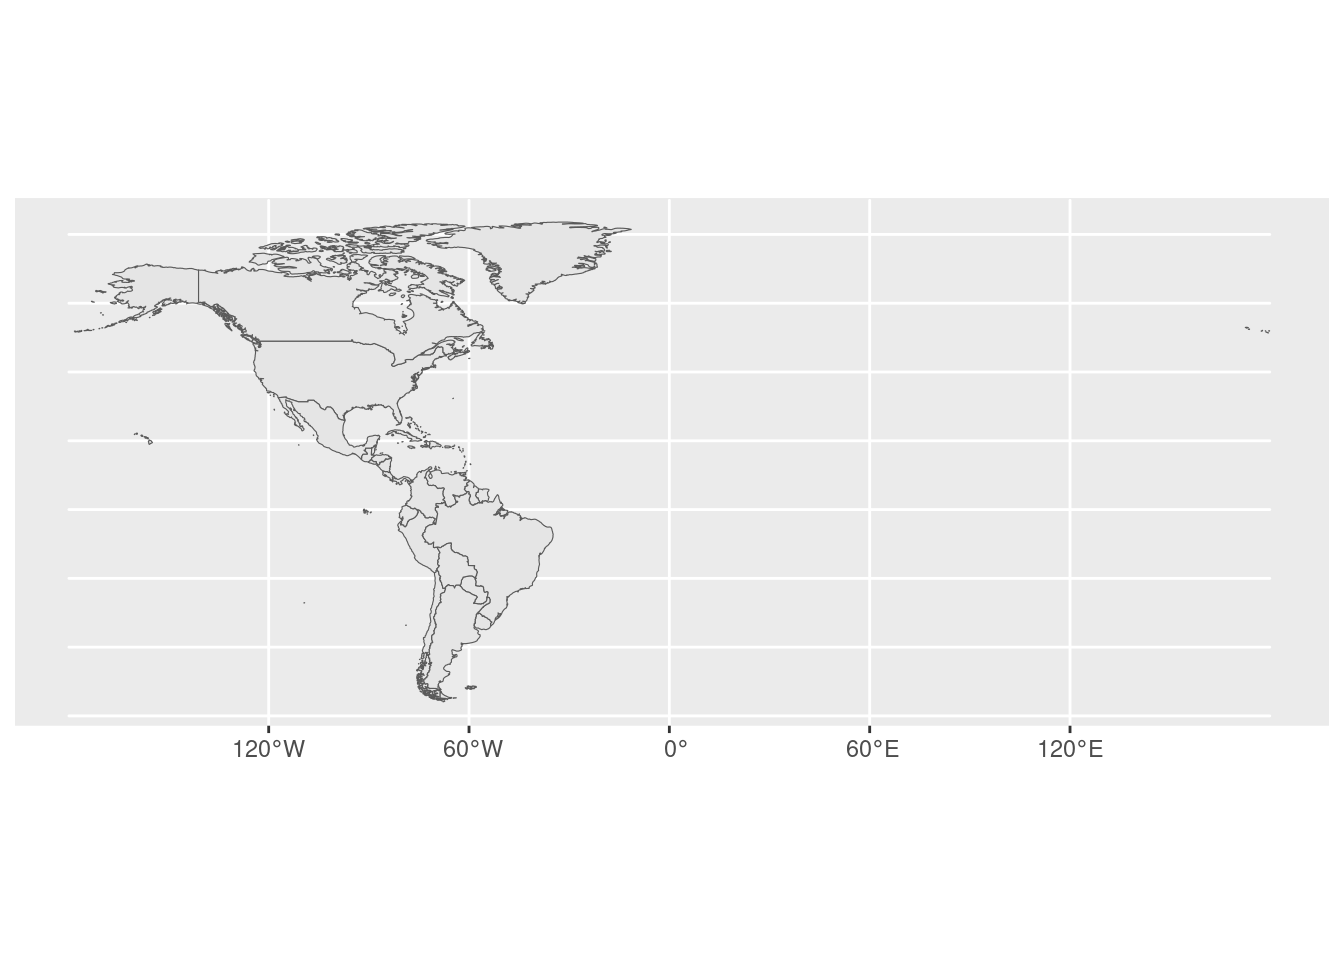
\includegraphics{bookdown_files/figure-latex/ambarom-americas-map-1.pdf}
\caption{\label{fig:ambarom-americas-map}Map of North and South America}
\end{figure}

The map in Figure \ref{fig:ambarom-americas-map} appears very wide due to the Aleutian islands in Alaska extending into the Eastern Hemisphere. We can crop the shapefile to include only the Western Hemisphere, which removes some of the trailing islands of Alaska.

\begin{Shaded}
\begin{Highlighting}[]
\NormalTok{country\_shape\_crop }\OtherTok{\textless{}{-}}\NormalTok{ country\_shape }\SpecialCharTok{\%\textgreater{}\%}
  \FunctionTok{st\_crop}\NormalTok{(}\FunctionTok{c}\NormalTok{(}
    \AttributeTok{xmin =} \SpecialCharTok{{-}}\DecValTok{180}\NormalTok{,}
    \AttributeTok{xmax =} \DecValTok{0}\NormalTok{,}
    \AttributeTok{ymin =} \SpecialCharTok{{-}}\DecValTok{90}\NormalTok{,}
    \AttributeTok{ymax =} \DecValTok{90}
\NormalTok{  ))}
\end{Highlighting}
\end{Shaded}

Now that we have the necessary shape files, our next step is to match our survey data to the map. Countries can be named differently (e.g., ``U.S'', ``U.S.A'', ``United States''). To make sure we can visualize our survey data on the map, we need to match the country names in both the survey data and the map data. To do this, we can use the \texttt{anti\_join()} function to identify the countries in the survey data that aren't in the map data. For example, as shown below, the United States is referred to as ``United States'' in the survey data but ``United States of America'' in the map data. Table \ref{tab:ambarom-map-merge-check-1-tab} shows the countries in the survey data but not the map data and Table \ref{tab:ambarom-map-merge-check-2-tab} shows the countries in the map data but not the survey data.

\begin{Shaded}
\begin{Highlighting}[]
\NormalTok{survey\_country\_list }\OtherTok{\textless{}{-}}\NormalTok{ ambarom }\SpecialCharTok{\%\textgreater{}\%} \FunctionTok{distinct}\NormalTok{(Country)}

\NormalTok{survey\_country\_list\_gt }\OtherTok{\textless{}{-}}\NormalTok{ survey\_country\_list }\SpecialCharTok{\%\textgreater{}\%}
  \FunctionTok{anti\_join}\NormalTok{(country\_shape\_crop, }\AttributeTok{by =} \FunctionTok{c}\NormalTok{(}\StringTok{"Country"} \OtherTok{=} \StringTok{"geounit"}\NormalTok{)) }\SpecialCharTok{\%\textgreater{}\%}
  \FunctionTok{gt}\NormalTok{()}
\end{Highlighting}
\end{Shaded}

\begin{Shaded}
\begin{Highlighting}[]
\NormalTok{survey\_country\_list\_gt}
\end{Highlighting}
\end{Shaded}



\begin{longtable}{c}
\caption{\label{tab:ambarom-map-merge-check-1-tab}Countries in the survey data but not the map data}\\
\toprule
Country \\ 
\midrule
United States \\ 
\bottomrule
\end{longtable}

\begin{Shaded}
\begin{Highlighting}[]
\NormalTok{map\_country\_list\_gt }\OtherTok{\textless{}{-}}\NormalTok{ country\_shape\_crop }\SpecialCharTok{\%\textgreater{}\%}
  \FunctionTok{as\_tibble}\NormalTok{() }\SpecialCharTok{\%\textgreater{}\%}
  \FunctionTok{select}\NormalTok{(geounit, sovereignt) }\SpecialCharTok{\%\textgreater{}\%}
  \FunctionTok{anti\_join}\NormalTok{(survey\_country\_list, }\AttributeTok{by =} \FunctionTok{c}\NormalTok{(}\StringTok{"geounit"} \OtherTok{=} \StringTok{"Country"}\NormalTok{)) }\SpecialCharTok{\%\textgreater{}\%}
  \FunctionTok{arrange}\NormalTok{(geounit) }\SpecialCharTok{\%\textgreater{}\%}
  \FunctionTok{gt}\NormalTok{()}
\end{Highlighting}
\end{Shaded}

\begin{Shaded}
\begin{Highlighting}[]
\NormalTok{map\_country\_list\_gt}
\end{Highlighting}
\end{Shaded}



\begin{longtable}{ll}
\caption{\label{tab:ambarom-map-merge-check-2-tab}Countries in the map data but not the survey data}\\
\toprule
geounit & sovereignt \\ 
\midrule
Anguilla & United Kingdom \\ 
Antigua and Barbuda & Antigua and Barbuda \\ 
Aruba & Netherlands \\ 
Barbados & Barbados \\ 
Belize & Belize \\ 
Bermuda & United Kingdom \\ 
British Virgin Islands & United Kingdom \\ 
Cayman Islands & United Kingdom \\ 
Cuba & Cuba \\ 
Curaçao & Netherlands \\ 
Dominica & Dominica \\ 
Falkland Islands & United Kingdom \\ 
Greenland & Denmark \\ 
Grenada & Grenada \\ 
Montserrat & United Kingdom \\ 
Puerto Rico & United States of America \\ 
Saint Barthelemy & France \\ 
Saint Kitts and Nevis & Saint Kitts and Nevis \\ 
Saint Lucia & Saint Lucia \\ 
Saint Martin & France \\ 
Saint Pierre and Miquelon & France \\ 
Saint Vincent and the Grenadines & Saint Vincent and the Grenadines \\ 
Sint Maarten & Netherlands \\ 
Suriname & Suriname \\ 
The Bahamas & The Bahamas \\ 
Trinidad and Tobago & Trinidad and Tobago \\ 
Turks and Caicos Islands & United Kingdom \\ 
United States Virgin Islands & United States of America \\ 
United States of America & United States of America \\ 
Venezuela & Venezuela \\ 
\bottomrule
\end{longtable}

There are several ways to fix the mismatched names for a successful join. The simplest solution is to rename the data in the shape object before merging. Since only one country name in the survey data differs from the map data, we rename the map data accordingly.

\begin{Shaded}
\begin{Highlighting}[]
\NormalTok{country\_shape\_upd }\OtherTok{\textless{}{-}}\NormalTok{ country\_shape\_crop }\SpecialCharTok{\%\textgreater{}\%}
  \FunctionTok{mutate}\NormalTok{(}\AttributeTok{geounit =} \FunctionTok{if\_else}\NormalTok{(geounit }\SpecialCharTok{==} \StringTok{"United States of America"}\NormalTok{,}
    \StringTok{"United States"}\NormalTok{, geounit}
\NormalTok{  ))}
\end{Highlighting}
\end{Shaded}

Now that the country names match, we can merge the survey and map data and then plot the data. We begin with the map file and merge it with the survey estimates generated in Section \ref{ambarom-estimates} (\texttt{covid\_worry\_country\_ests} and \texttt{covid\_educ\_ests}). We use the tidyverse function of \texttt{full\_join()}, which joins the rows in the map data and the survey estimates based on the columns \texttt{geounit} and \texttt{Country}. A full join keeps all the rows from both datasets, matching rows when possible. For any rows without matches, the function fills in an \texttt{NA} for the missing value.

\begin{Shaded}
\begin{Highlighting}[]
\NormalTok{covid\_sf }\OtherTok{\textless{}{-}}\NormalTok{ country\_shape\_upd }\SpecialCharTok{\%\textgreater{}\%}
  \FunctionTok{full\_join}\NormalTok{(covid\_worry\_country\_ests,}
    \AttributeTok{by =} \FunctionTok{c}\NormalTok{(}\StringTok{"geounit"} \OtherTok{=} \StringTok{"Country"}\NormalTok{)}
\NormalTok{  ) }\SpecialCharTok{\%\textgreater{}\%}
  \FunctionTok{full\_join}\NormalTok{(covid\_educ\_ests,}
    \AttributeTok{by =} \FunctionTok{c}\NormalTok{(}\StringTok{"geounit"} \OtherTok{=} \StringTok{"Country"}\NormalTok{)}
\NormalTok{  )}
\end{Highlighting}
\end{Shaded}

After the merge, we create two figures that display the population estimates for the percentage of people worried about COVID (Figure \ref{fig:ambarom-make-maps-covid}) and the percentage of households with at least one child participating in virtual or hybrid learning (Figure \ref{fig:ambarom-make-maps-covid-ed}).

\begin{Shaded}
\begin{Highlighting}[]
\FunctionTok{ggplot}\NormalTok{() }\SpecialCharTok{+}
  \FunctionTok{geom\_sf}\NormalTok{(}
    \AttributeTok{data =}\NormalTok{ covid\_sf,}
    \FunctionTok{aes}\NormalTok{(}\AttributeTok{fill =}\NormalTok{ p, }\AttributeTok{geometry =}\NormalTok{ geometry),}
    \AttributeTok{color =} \StringTok{"darkgray"}
\NormalTok{  ) }\SpecialCharTok{+}
  \FunctionTok{scale\_fill\_gradientn}\NormalTok{(}
    \AttributeTok{guide =} \StringTok{"colorbar"}\NormalTok{,}
    \AttributeTok{name =} \StringTok{"Percent"}\NormalTok{,}
    \AttributeTok{labels =}\NormalTok{ scales}\SpecialCharTok{::}\NormalTok{comma,}
    \AttributeTok{colors =} \FunctionTok{c}\NormalTok{(}\StringTok{"\#BFD7EA"}\NormalTok{, }\StringTok{"\#087e8b"}\NormalTok{, }\StringTok{"\#0B3954"}\NormalTok{),}
    \AttributeTok{na.value =} \ConstantTok{NA}
\NormalTok{  ) }\SpecialCharTok{+}
  \FunctionTok{geom\_sf\_pattern}\NormalTok{(}
    \AttributeTok{data =} \FunctionTok{filter}\NormalTok{(covid\_sf, }\FunctionTok{is.na}\NormalTok{(p)),}
    \AttributeTok{pattern =} \StringTok{"crosshatch"}\NormalTok{,}
    \AttributeTok{pattern\_fill =} \StringTok{"lightgray"}\NormalTok{,}
    \AttributeTok{pattern\_color =} \StringTok{"lightgray"}\NormalTok{,}
    \AttributeTok{fill =} \ConstantTok{NA}\NormalTok{,}
    \AttributeTok{color =} \StringTok{"darkgray"}
\NormalTok{  ) }\SpecialCharTok{+}
  \FunctionTok{theme\_minimal}\NormalTok{()}
\end{Highlighting}
\end{Shaded}

\begin{figure}
\centering
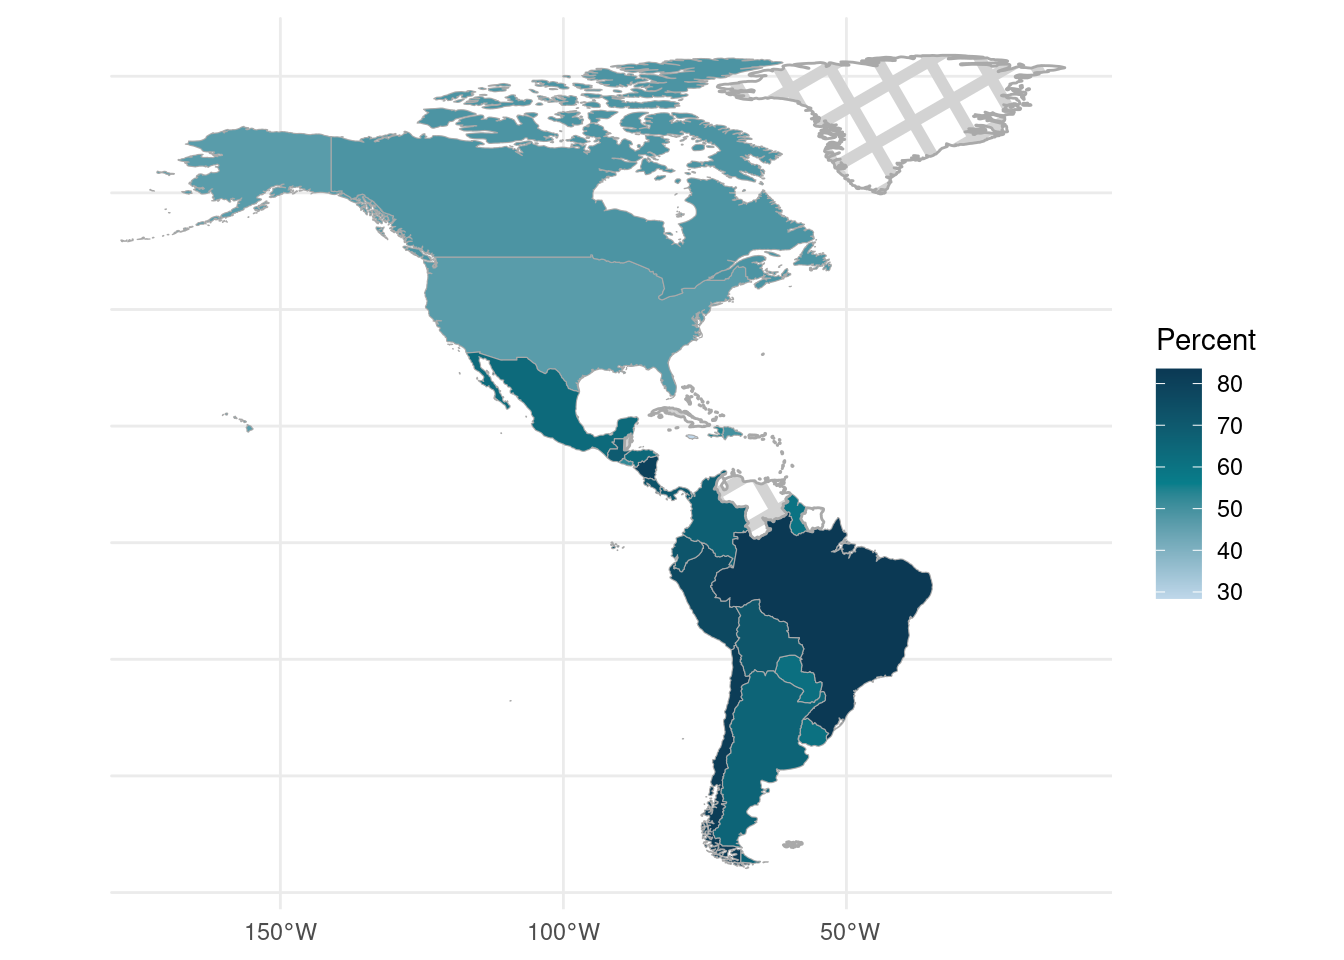
\includegraphics{bookdown_files/figure-latex/ambarom-make-maps-covid-1.pdf}
\caption{\label{fig:ambarom-make-maps-covid}Percent of households worried someone in their household will get COVID-19 in the next 3 months by country}
\end{figure}

\begin{Shaded}
\begin{Highlighting}[]
\FunctionTok{ggplot}\NormalTok{() }\SpecialCharTok{+}
  \FunctionTok{geom\_sf}\NormalTok{(}
    \AttributeTok{data =}\NormalTok{ covid\_sf,}
    \FunctionTok{aes}\NormalTok{(}\AttributeTok{fill =}\NormalTok{ p\_mediumchange, }\AttributeTok{geometry =}\NormalTok{ geometry),}
    \AttributeTok{color =} \StringTok{"darkgray"}
\NormalTok{  ) }\SpecialCharTok{+}
  \FunctionTok{scale\_fill\_gradientn}\NormalTok{(}
    \AttributeTok{guide =} \StringTok{"colorbar"}\NormalTok{,}
    \AttributeTok{name =} \StringTok{"Percent"}\NormalTok{,}
    \AttributeTok{labels =}\NormalTok{ scales}\SpecialCharTok{::}\NormalTok{comma,}
    \AttributeTok{colors =} \FunctionTok{c}\NormalTok{(}\StringTok{"\#BFD7EA"}\NormalTok{, }\StringTok{"\#087e8b"}\NormalTok{, }\StringTok{"\#0B3954"}\NormalTok{),}
    \AttributeTok{na.value =} \ConstantTok{NA}
\NormalTok{  ) }\SpecialCharTok{+}
  \FunctionTok{geom\_sf\_pattern}\NormalTok{(}
    \AttributeTok{data =} \FunctionTok{filter}\NormalTok{(covid\_sf, }\FunctionTok{is.na}\NormalTok{(p\_mediumchange)),}
    \AttributeTok{pattern =} \StringTok{"crosshatch"}\NormalTok{,}
    \AttributeTok{pattern\_fill =} \StringTok{"lightgray"}\NormalTok{,}
    \AttributeTok{pattern\_color =} \StringTok{"lightgray"}\NormalTok{,}
    \AttributeTok{fill =} \ConstantTok{NA}\NormalTok{,}
    \AttributeTok{color =} \StringTok{"darkgray"}
\NormalTok{  ) }\SpecialCharTok{+}
  \FunctionTok{theme\_minimal}\NormalTok{()}
\end{Highlighting}
\end{Shaded}

\begin{figure}
\centering
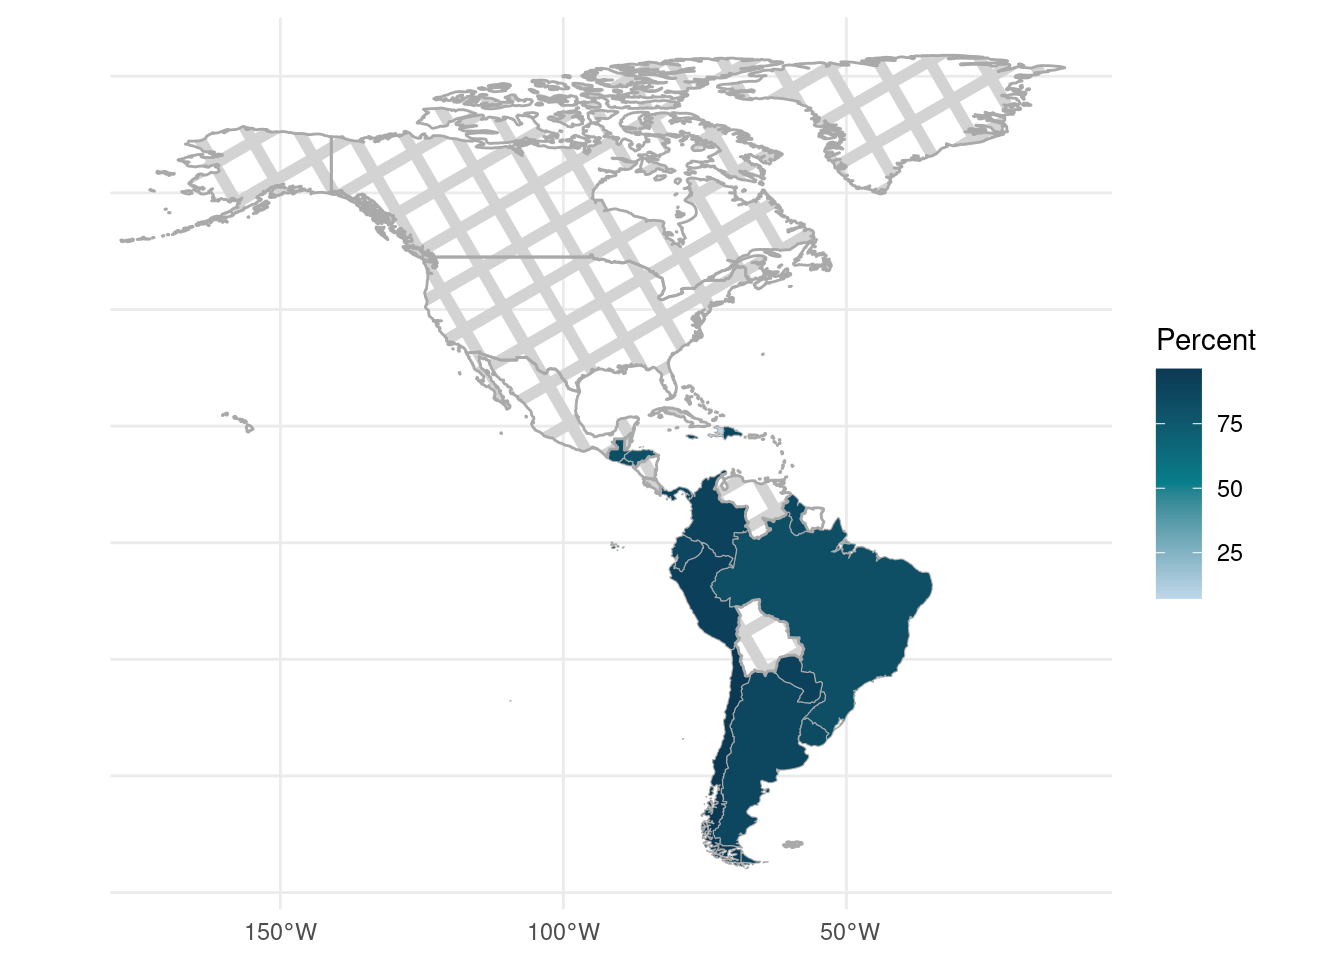
\includegraphics{bookdown_files/figure-latex/ambarom-make-maps-covid-ed-1.pdf}
\caption{\label{fig:ambarom-make-maps-covid-ed}Percent of households who had at least one child participate in virtual or hybrid learning}
\end{figure}

In Figure \ref{fig:ambarom-make-maps-covid-ed}, we observe missing data (represented by the crosshatch pattern) for Canada, Mexico, and the United States. The questionnaires indicate that these three countries did not include the education question in the survey. To focus on countries with available data, we can remove North America from the map and show only Central and South America. We do this below by restricting the shape files to Latin America and the Caribbean, as depicted in Figure \ref{fig:ambarom-make-maps-covid-ed-c-s}.

\begin{Shaded}
\begin{Highlighting}[]
\NormalTok{covid\_c\_s }\OtherTok{\textless{}{-}}\NormalTok{ covid\_sf }\SpecialCharTok{\%\textgreater{}\%}
  \FunctionTok{filter}\NormalTok{(region\_wb }\SpecialCharTok{==} \StringTok{"Latin America \& Caribbean"}\NormalTok{)}

\FunctionTok{ggplot}\NormalTok{() }\SpecialCharTok{+}
  \FunctionTok{geom\_sf}\NormalTok{(}
    \AttributeTok{data =}\NormalTok{ covid\_c\_s,}
    \FunctionTok{aes}\NormalTok{(}\AttributeTok{fill =}\NormalTok{ p\_mediumchange, }\AttributeTok{geometry =}\NormalTok{ geometry),}
    \AttributeTok{color =} \StringTok{"darkgray"}
\NormalTok{  ) }\SpecialCharTok{+}
  \FunctionTok{scale\_fill\_gradientn}\NormalTok{(}
    \AttributeTok{guide =} \StringTok{"colorbar"}\NormalTok{,}
    \AttributeTok{name =} \StringTok{"Percent"}\NormalTok{,}
    \AttributeTok{labels =}\NormalTok{ scales}\SpecialCharTok{::}\NormalTok{comma,}
    \AttributeTok{colors =} \FunctionTok{c}\NormalTok{(}\StringTok{"\#BFD7EA"}\NormalTok{, }\StringTok{"\#087e8b"}\NormalTok{, }\StringTok{"\#0B3954"}\NormalTok{),}
    \AttributeTok{na.value =} \ConstantTok{NA}
\NormalTok{  ) }\SpecialCharTok{+}
  \FunctionTok{geom\_sf\_pattern}\NormalTok{(}
    \AttributeTok{data =} \FunctionTok{filter}\NormalTok{(covid\_c\_s, }\FunctionTok{is.na}\NormalTok{(p\_mediumchange)),}
    \AttributeTok{pattern =} \StringTok{"crosshatch"}\NormalTok{,}
    \AttributeTok{pattern\_fill =} \StringTok{"lightgray"}\NormalTok{,}
    \AttributeTok{pattern\_color =} \StringTok{"lightgray"}\NormalTok{,}
    \AttributeTok{fill =} \ConstantTok{NA}\NormalTok{,}
    \AttributeTok{color =} \StringTok{"darkgray"}
\NormalTok{  ) }\SpecialCharTok{+}
  \FunctionTok{theme\_minimal}\NormalTok{()}
\end{Highlighting}
\end{Shaded}

\begin{figure}
\centering
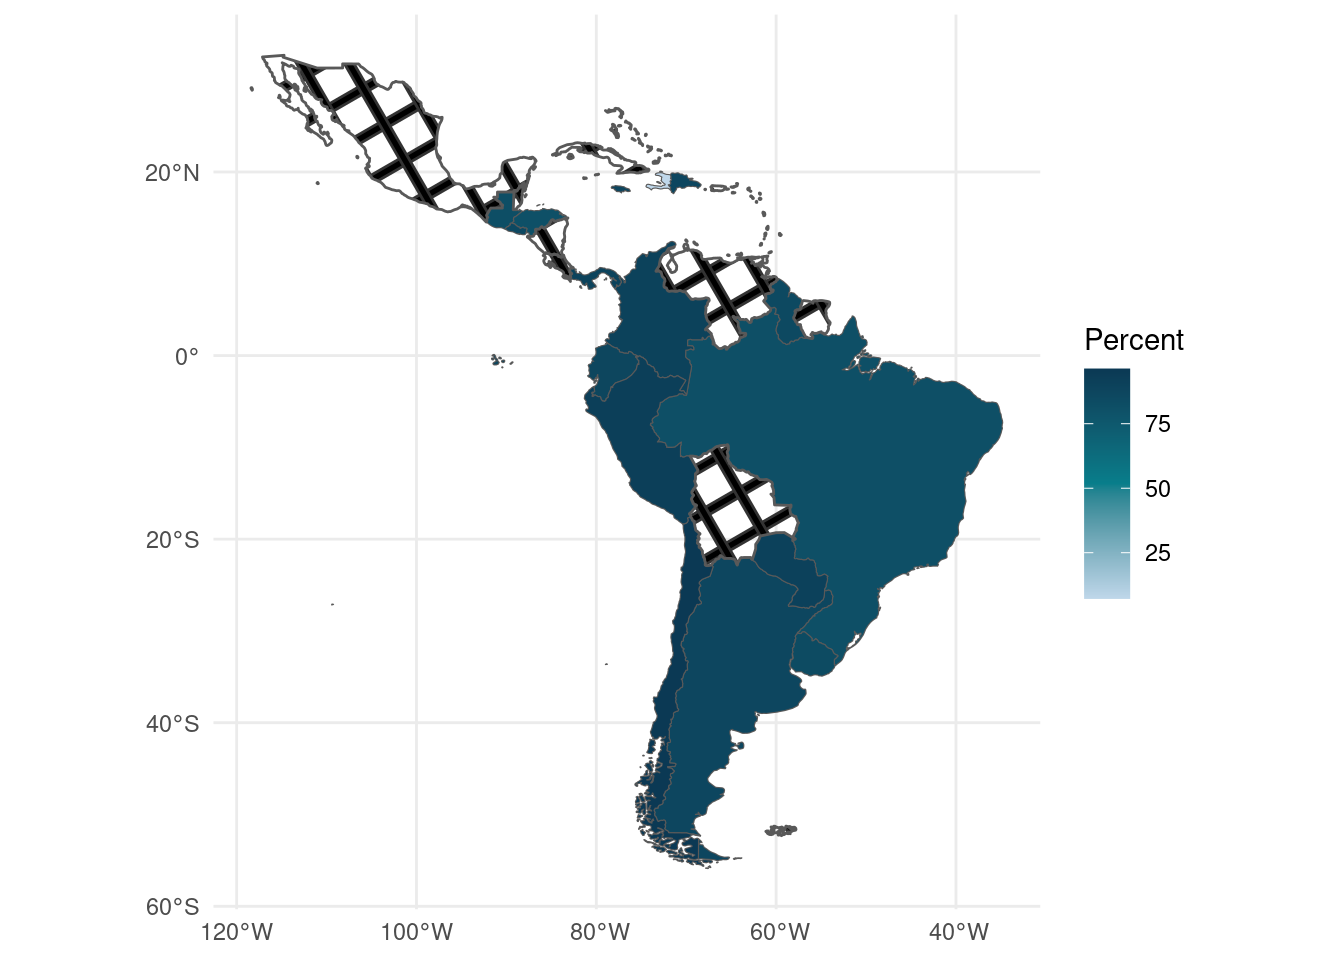
\includegraphics{bookdown_files/figure-latex/ambarom-make-maps-covid-ed-c-s-1.pdf}
\caption{\label{fig:ambarom-make-maps-covid-ed-c-s}Percent of households who had at least one child participate in virtual or hybrid learning, Central and South America}
\end{figure}

In Figure \ref{fig:ambarom-make-maps-covid-ed-c-s}, we can see that most countries with available data have similar percentages (reflected in their similar shades). However, Haiti stands out with a lighter shade, indicating a considerably lower percentage of households with at least one child participating in virtual or hybrid learning.

\hypertarget{exercises-4}{%
\section{Exercises}\label{exercises-4}}

\begin{enumerate}
\def\labelenumi{\arabic{enumi}.}
\tightlist
\item
  Calculate the percentage of households with broadband internet and those with any internet at home, including from a phone or tablet. Hint: if you come across countries with 0\% internet usage, you may want to filter by something first.
\end{enumerate}

\begin{Shaded}
\begin{Highlighting}[]
\NormalTok{int\_ests }\OtherTok{\textless{}{-}}
\NormalTok{  ambarom\_des }\SpecialCharTok{\%\textgreater{}\%}
  \FunctionTok{filter}\NormalTok{(}\SpecialCharTok{!}\FunctionTok{is.na}\NormalTok{(Internet) }\SpecialCharTok{|} \SpecialCharTok{!}\FunctionTok{is.na}\NormalTok{(BroadbandInternet)) }\SpecialCharTok{\%\textgreater{}\%}
  \FunctionTok{group\_by}\NormalTok{(Country) }\SpecialCharTok{\%\textgreater{}\%}
  \FunctionTok{summarize}\NormalTok{(}
    \AttributeTok{p\_broadband =} \FunctionTok{survey\_mean}\NormalTok{(BroadbandInternet, }\AttributeTok{na.rm =} \ConstantTok{TRUE}\NormalTok{) }\SpecialCharTok{*} \DecValTok{100}\NormalTok{,}
    \AttributeTok{p\_internet =} \FunctionTok{survey\_mean}\NormalTok{(Internet, }\AttributeTok{na.rm =} \ConstantTok{TRUE}\NormalTok{) }\SpecialCharTok{*} \DecValTok{100}
\NormalTok{  )}

\NormalTok{int\_ests }\SpecialCharTok{\%\textgreater{}\%}
  \FunctionTok{print}\NormalTok{(}\AttributeTok{n =} \DecValTok{30}\NormalTok{)}
\end{Highlighting}
\end{Shaded}

\begin{verbatim}
## # A tibble: 20 x 5
##    Country           p_broadband p_broadband_se p_internet p_internet_se
##    <fct>                   <dbl>          <dbl>      <dbl>         <dbl>
##  1 Argentina                62.3          1.13        86.2         0.871
##  2 Bolivia                  41.4          1.03        77.2         0.956
##  3 Brazil                   68.3          1.25        88.9         0.879
##  4 Chile                    63.1          1.06        93.5         0.550
##  5 Colombia                 45.7          1.15        68.7         1.09 
##  6 Costa Rica               49.6          1.07        84.4         0.798
##  7 Dominican Republ~        37.1          1.04        73.7         1.05 
##  8 Ecuador                  59.7          1.06        79.9         0.898
##  9 El Salvador              30.2          0.906       63.9         0.985
## 10 Guatemala                33.4          0.993       61.5         1.08 
## 11 Guyana                   63.7          1.09        86.8         0.781
## 12 Haiti                    11.8          0.791       58.5         1.25 
## 13 Honduras                 28.2          0.968       60.7         1.11 
## 14 Jamaica                  64.2          0.986       91.5         0.602
## 15 Mexico                   44.9          1.05        70.9         1.05 
## 16 Nicaragua                39.1          1.12        76.3         1.09 
## 17 Panama                   43.4          1.02        73.1         0.976
## 18 Paraguay                 33.3          0.971       72.9         1.01 
## 19 Peru                     42.4          1.07        71.1         1.07 
## 20 Uruguay                  62.7          1.08        90.6         0.699
\end{verbatim}

\begin{enumerate}
\def\labelenumi{\arabic{enumi}.}
\setcounter{enumi}{1}
\tightlist
\item
  Create a faceted map showing both broadband internet and any internet usage.
\end{enumerate}

\begin{Shaded}
\begin{Highlighting}[]
\NormalTok{internet\_sf }\OtherTok{\textless{}{-}}\NormalTok{ country\_shape\_upd }\SpecialCharTok{\%\textgreater{}\%}
  \FunctionTok{full\_join}\NormalTok{(}\FunctionTok{select}\NormalTok{(int\_ests, }\AttributeTok{p =}\NormalTok{ p\_internet, }\AttributeTok{geounit =}\NormalTok{ Country), }\AttributeTok{by =} \StringTok{"geounit"}\NormalTok{) }\SpecialCharTok{\%\textgreater{}\%}
  \FunctionTok{mutate}\NormalTok{(}\AttributeTok{Type =} \StringTok{"Internet"}\NormalTok{)}
\NormalTok{broadband\_sf }\OtherTok{\textless{}{-}}\NormalTok{ country\_shape\_upd }\SpecialCharTok{\%\textgreater{}\%}
  \FunctionTok{full\_join}\NormalTok{(}\FunctionTok{select}\NormalTok{(int\_ests, }\AttributeTok{p =}\NormalTok{ p\_broadband, }\AttributeTok{geounit =}\NormalTok{ Country), }\AttributeTok{by =} \StringTok{"geounit"}\NormalTok{) }\SpecialCharTok{\%\textgreater{}\%}
  \FunctionTok{mutate}\NormalTok{(}\AttributeTok{Type =} \StringTok{"Broadband"}\NormalTok{)}
\NormalTok{b\_int\_sf }\OtherTok{\textless{}{-}}\NormalTok{ internet\_sf }\SpecialCharTok{\%\textgreater{}\%}
  \FunctionTok{bind\_rows}\NormalTok{(broadband\_sf) }\SpecialCharTok{\%\textgreater{}\%}
  \FunctionTok{filter}\NormalTok{(region\_wb }\SpecialCharTok{==} \StringTok{"Latin America \& Caribbean"}\NormalTok{)}

\NormalTok{b\_int\_sf }\SpecialCharTok{\%\textgreater{}\%}
  \FunctionTok{ggplot}\NormalTok{(}\FunctionTok{aes}\NormalTok{(}\AttributeTok{fill =}\NormalTok{ p),}
    \AttributeTok{color =} \StringTok{"darkgray"}
\NormalTok{  ) }\SpecialCharTok{+}
  \FunctionTok{geom\_sf}\NormalTok{() }\SpecialCharTok{+}
  \FunctionTok{facet\_wrap}\NormalTok{(}\SpecialCharTok{\textasciitilde{}}\NormalTok{Type) }\SpecialCharTok{+}
  \FunctionTok{scale\_fill\_gradientn}\NormalTok{(}
    \AttributeTok{guide =} \StringTok{"colorbar"}\NormalTok{,}
    \AttributeTok{name =} \StringTok{"Percent"}\NormalTok{,}
    \AttributeTok{labels =}\NormalTok{ scales}\SpecialCharTok{::}\NormalTok{comma,}
    \AttributeTok{colors =} \FunctionTok{c}\NormalTok{(}\StringTok{"\#BFD7EA"}\NormalTok{, }\StringTok{"\#087E8B"}\NormalTok{, }\StringTok{"\#0B3954"}\NormalTok{),}
    \AttributeTok{na.value =} \ConstantTok{NA}
\NormalTok{  ) }\SpecialCharTok{+}
  \FunctionTok{geom\_sf\_pattern}\NormalTok{(}
    \AttributeTok{data =} \FunctionTok{filter}\NormalTok{(b\_int\_sf, }\FunctionTok{is.na}\NormalTok{(p)),}
    \AttributeTok{pattern =} \StringTok{"crosshatch"}\NormalTok{,}
    \AttributeTok{pattern\_fill =} \StringTok{"lightgray"}\NormalTok{,}
    \AttributeTok{pattern\_color =} \StringTok{"lightgray"}\NormalTok{,}
    \AttributeTok{fill =} \ConstantTok{NA}\NormalTok{,}
    \AttributeTok{color =} \StringTok{"darkgray"}
\NormalTok{  ) }\SpecialCharTok{+}
  \FunctionTok{theme\_minimal}\NormalTok{()}
\end{Highlighting}
\end{Shaded}

\begin{figure}
\centering
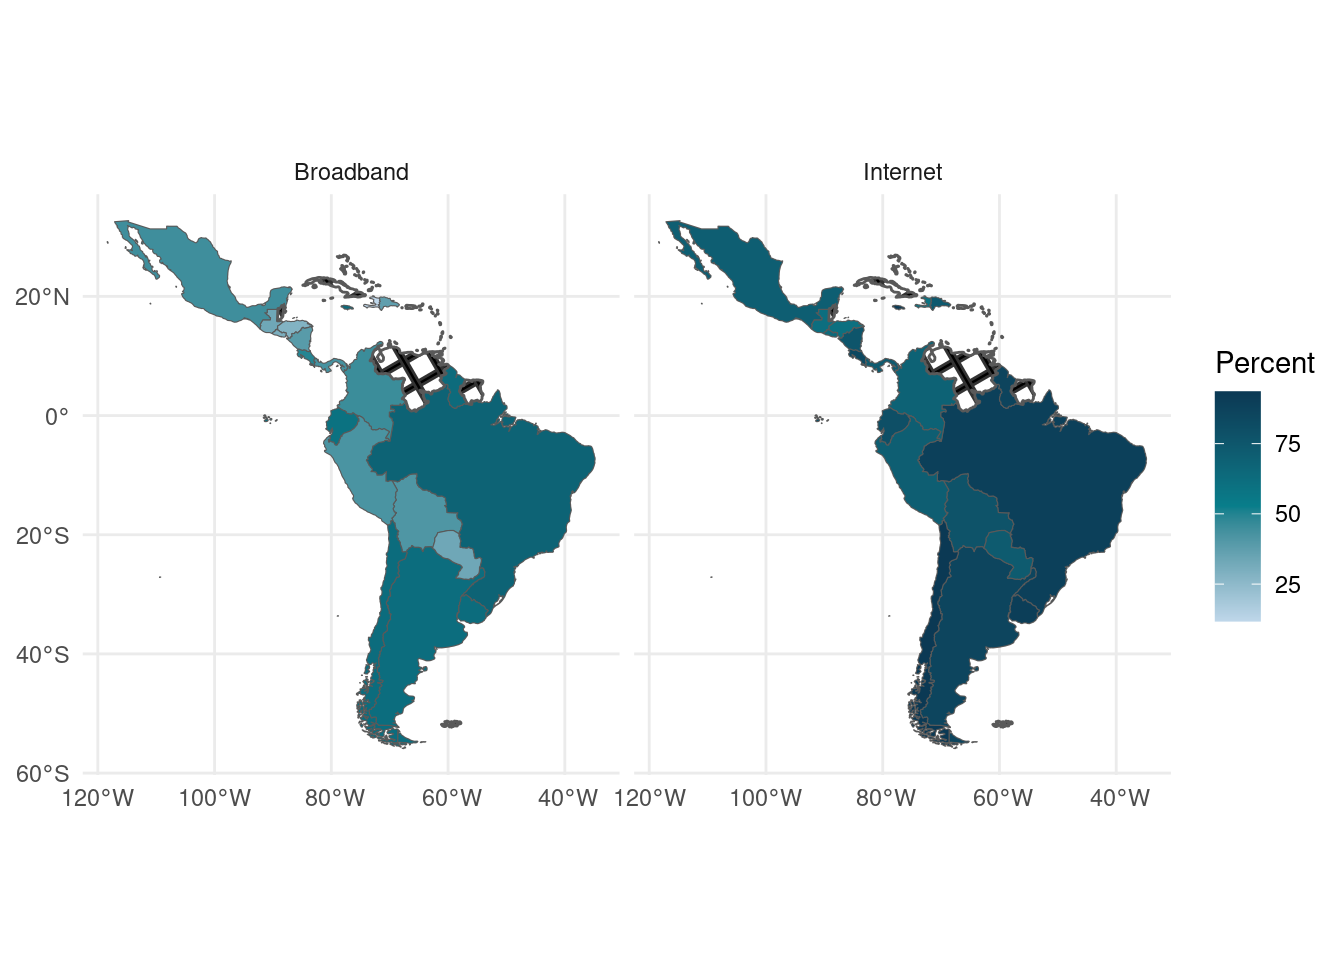
\includegraphics{bookdown_files/figure-latex/ambarom-facet-map-1.pdf}
\caption{\label{fig:ambarom-facet-map}Percent of broadband internet and any internet usage, Central and South America}
\end{figure}

\cleardoublepage

\hypertarget{appendix-appendices}{%
\appendix \addcontentsline{toc}{chapter}{\appendixname}}


\hypertarget{anes-cb}{%
\chapter{ANES Derived Variable Codebook}\label{anes-cb}}

The full codebook with the original variables is available at \url{https://electionstudies.org/wp-content/uploads/2022/02/anes_timeseries_2020_userguidecodebook_20220210.pdf}

\hypertarget{admin}{%
\section{ADMIN}\label{admin}}

\hypertarget{v200001}{%
\subsubsection*{V200001}\label{v200001}}


Description: 2020 Case ID

Variable class: numeric

\hypertarget{caseid}{%
\subsubsection*{CaseID}\label{caseid}}


Description: 2020 Case ID

Variable class: numeric

\hypertarget{v200002}{%
\subsubsection*{V200002}\label{v200002}}


Description: Mode~of~interview:~pre-election~interview

Variable class: haven\_labelled, vctrs\_vctr, double

\begin{tabular}[t]{l|l|r|r}
\hline
V200002 & Label & n & Unweighted Freq\\
\hline
1 & 1. Video & 274 & 0.037\\
\hline
2 & 2. Telephone & 115 & 0.015\\
\hline
3 & 3. Web & 7064 & 0.948\\
\hline
Total & - & 7453 & 1.000\\
\hline
\end{tabular}

\hypertarget{interviewmode}{%
\subsubsection*{InterviewMode}\label{interviewmode}}


Description: Mode~of~interview:~pre-election~interview

Variable class: factor

\begin{tabular}[t]{l|r|r}
\hline
InterviewMode & n & Unweighted Freq\\
\hline
Video & 274 & 0.037\\
\hline
Telephone & 115 & 0.015\\
\hline
Web & 7064 & 0.948\\
\hline
Total & 7453 & 1.000\\
\hline
\end{tabular}

\hypertarget{weights}{%
\section{WEIGHTS}\label{weights}}

\hypertarget{v200010b}{%
\subsubsection*{V200010b}\label{v200010b}}


Description: Full~sample~post-election~weight

Variable class: numeric

\begin{tabular}[t]{r|r|r|r}
\hline
N Missing & Minimum & Median & Maximum\\
\hline
0 & 0.0083 & 0.6863 & 6.651\\
\hline
\end{tabular}

\hypertarget{weight}{%
\subsubsection*{Weight}\label{weight}}


Description: Full~sample~post-election~weight

Variable class: numeric

\begin{tabular}[t]{r|r|r|r}
\hline
N Missing & Minimum & Median & Maximum\\
\hline
0 & 0.0083 & 0.6863 & 6.651\\
\hline
\end{tabular}

\hypertarget{v200010c}{%
\subsubsection*{V200010c}\label{v200010c}}


Description: Full~sample~variance~unit

Variable class: numeric

\begin{tabular}[t]{r|r|r|r}
\hline
N Missing & Minimum & Median & Maximum\\
\hline
0 & 1 & 2 & 3\\
\hline
\end{tabular}

\hypertarget{varunit}{%
\subsubsection*{VarUnit}\label{varunit}}


Description: Full~sample~variance~unit

Variable class: factor

\begin{tabular}[t]{l|r|r}
\hline
VarUnit & n & Unweighted Freq\\
\hline
1 & 3689 & 0.495\\
\hline
2 & 3750 & 0.503\\
\hline
3 & 14 & 0.002\\
\hline
Total & 7453 & 1.000\\
\hline
\end{tabular}

\hypertarget{v200010d}{%
\subsubsection*{V200010d}\label{v200010d}}


Description: Full~sample~variance~stratum

Variable class: numeric

\begin{tabular}[t]{r|r|r|r}
\hline
N Missing & Minimum & Median & Maximum\\
\hline
0 & 1 & 24 & 50\\
\hline
\end{tabular}

\hypertarget{stratum}{%
\subsubsection*{Stratum}\label{stratum}}


Description: Full~sample~variance~stratum

Variable class: factor

\begin{tabular}[t]{l|r|r}
\hline
Stratum & n & Unweighted Freq\\
\hline
1 & 167 & 0.022\\
\hline
2 & 148 & 0.020\\
\hline
3 & 158 & 0.021\\
\hline
4 & 151 & 0.020\\
\hline
5 & 147 & 0.020\\
\hline
6 & 172 & 0.023\\
\hline
7 & 163 & 0.022\\
\hline
8 & 159 & 0.021\\
\hline
9 & 160 & 0.021\\
\hline
10 & 159 & 0.021\\
\hline
11 & 137 & 0.018\\
\hline
12 & 179 & 0.024\\
\hline
13 & 148 & 0.020\\
\hline
14 & 160 & 0.021\\
\hline
15 & 159 & 0.021\\
\hline
16 & 148 & 0.020\\
\hline
17 & 158 & 0.021\\
\hline
18 & 156 & 0.021\\
\hline
19 & 154 & 0.021\\
\hline
20 & 144 & 0.019\\
\hline
21 & 170 & 0.023\\
\hline
22 & 146 & 0.020\\
\hline
23 & 165 & 0.022\\
\hline
24 & 147 & 0.020\\
\hline
25 & 169 & 0.023\\
\hline
26 & 165 & 0.022\\
\hline
27 & 172 & 0.023\\
\hline
28 & 133 & 0.018\\
\hline
29 & 157 & 0.021\\
\hline
30 & 167 & 0.022\\
\hline
31 & 154 & 0.021\\
\hline
32 & 143 & 0.019\\
\hline
33 & 143 & 0.019\\
\hline
34 & 124 & 0.017\\
\hline
35 & 138 & 0.019\\
\hline
36 & 130 & 0.017\\
\hline
37 & 136 & 0.018\\
\hline
38 & 145 & 0.019\\
\hline
39 & 140 & 0.019\\
\hline
40 & 125 & 0.017\\
\hline
41 & 158 & 0.021\\
\hline
42 & 146 & 0.020\\
\hline
43 & 130 & 0.017\\
\hline
44 & 126 & 0.017\\
\hline
45 & 126 & 0.017\\
\hline
46 & 135 & 0.018\\
\hline
47 & 133 & 0.018\\
\hline
48 & 140 & 0.019\\
\hline
49 & 133 & 0.018\\
\hline
50 & 130 & 0.017\\
\hline
Total & 7453 & 1.000\\
\hline
\end{tabular}

\hypertarget{pre-election-survey-questionnaire}{%
\section{PRE-ELECTION SURVEY QUESTIONNAIRE}\label{pre-election-survey-questionnaire}}

\hypertarget{v201006}{%
\subsubsection*{V201006}\label{v201006}}


Description: PRE:~How~interested~in~following~campaigns

Question: Some people don't pay much attention to political campaigns. How about you? Would you say that you have been very much interested, somewhat interested or not much interested in the political campaigns so far this year?

Variable class: haven\_labelled, vctrs\_vctr, double

\begin{tabular}[t]{l|l|r|r}
\hline
V201006 & Label & n & Unweighted Freq\\
\hline
-9 & -9. Refused & 1 & 0.000\\
\hline
1 & 1. Very much interested & 3940 & 0.529\\
\hline
2 & 2. Somewhat interested & 2569 & 0.345\\
\hline
3 & 3. Not much interested & 943 & 0.127\\
\hline
Total & - & 7453 & 1.000\\
\hline
\end{tabular}

\hypertarget{campaigninterest}{%
\subsubsection*{CampaignInterest}\label{campaigninterest}}


Description: PRE:~How~interested~in~following~campaigns

Question: Some people don't pay much attention to political campaigns. How about you? Would you say that you have been very much interested, somewhat interested or not much interested in the political campaigns so far this year?

Variable class: factor

\begin{tabular}[t]{l|r|r}
\hline
CampaignInterest & n & Unweighted Freq\\
\hline
Very much interested & 3940 & 0.529\\
\hline
Somewhat interested & 2569 & 0.345\\
\hline
Not much interested & 943 & 0.127\\
\hline
NA & 1 & 0.000\\
\hline
Total & 7453 & 1.000\\
\hline
\end{tabular}

\hypertarget{v201023}{%
\subsubsection*{V201023}\label{v201023}}


Description: PRE: Confirmation voted (early) in November 3 Election (2020)

Question: Just to be clear, I'm recording that you already voted in the election that is scheduled to take place on November 3. Is that right?

Variable class: haven\_labelled, vctrs\_vctr, double

\begin{tabular}[t]{l|l|r|r}
\hline
V201023 & Label & n & Unweighted Freq\\
\hline
-9 & -9. Refused & 2 & 0.000\\
\hline
-1 & -1. Inapplicable & 6961 & 0.934\\
\hline
1 & 1. Yes, voted & 375 & 0.050\\
\hline
2 & 2. No, have not voted & 115 & 0.015\\
\hline
Total & - & 7453 & 1.000\\
\hline
\end{tabular}

\hypertarget{earlyvote2020}{%
\subsubsection*{EarlyVote2020}\label{earlyvote2020}}


Description: PRE: Confirmation voted (early) in November 3 Election (2020)

Question: Just to be clear, I'm recording that you already voted in the election that is scheduled to take place on November 3. Is that right?

Variable class: factor

\begin{tabular}[t]{l|r|r}
\hline
EarlyVote2020 & n & Unweighted Freq\\
\hline
Yes & 375 & 0.050\\
\hline
No & 115 & 0.015\\
\hline
NA & 6963 & 0.934\\
\hline
Total & 7453 & 1.000\\
\hline
\end{tabular}

\hypertarget{v201024}{%
\subsubsection*{V201024}\label{v201024}}


Description: PRE: In what manner did R vote

Question: Which one of the following best describes how you voted?

Variable class: haven\_labelled, vctrs\_vctr, double

\begin{tabular}[t]{l|l|r|r}
\hline
V201024 & Label & n & Unweighted Freq\\
\hline
-9 & -9. Refused & 1 & 0.000\\
\hline
-1 & -1. Inapplicable & 7078 & 0.950\\
\hline
1 & 1. Definitely voted in person at a polling place before election day & 101 & 0.014\\
\hline
2 & 2. Definitely voted by mailing a ballot to elections officials before  election day & 242 & 0.032\\
\hline
3 & 3. Definitely voted in some other way & 28 & 0.004\\
\hline
4 & 4. Not completely sure whether you voted or not & 3 & 0.000\\
\hline
Total & - & 7453 & 1.000\\
\hline
\end{tabular}

\hypertarget{v201025x}{%
\subsubsection*{V201025x}\label{v201025x}}


Description: PRE:~SUMMARY:~Registration~and~early~vote~status

Variable class: haven\_labelled, vctrs\_vctr, double

\begin{tabular}[t]{l|l|r|r}
\hline
V201025x & Label & n & Unweighted Freq\\
\hline
-4 & -4. Technical error & 1 & 0.000\\
\hline
1 & 1. Not registered (or DK/RF), does not intend to register (or DK/RF intent) & 339 & 0.045\\
\hline
2 & 2. Not registered (or DK/RF), intends to register & 290 & 0.039\\
\hline
3 & 3. Registered but did not vote early (or DK/RF) & 6452 & 0.866\\
\hline
4 & 4. Registered and voted early & 371 & 0.050\\
\hline
Total & - & 7453 & 1.000\\
\hline
\end{tabular}

\hypertarget{v201028}{%
\subsubsection*{V201028}\label{v201028}}


Description: PRE: DID R VOTE FOR PRESIDENT

Question: How about the election for President? Did you vote for a candidate for President?

Variable class: haven\_labelled, vctrs\_vctr, double

\begin{tabular}[t]{l|l|r|r}
\hline
V201028 & Label & n & Unweighted Freq\\
\hline
-9 & -9. Refused & 1 & 0.000\\
\hline
-1 & -1. Inapplicable & 7081 & 0.950\\
\hline
1 & 1. Yes, voted for President & 361 & 0.048\\
\hline
2 & 2. No, didn't vote for President & 10 & 0.001\\
\hline
Total & - & 7453 & 1.000\\
\hline
\end{tabular}

\hypertarget{v201029}{%
\subsubsection*{V201029}\label{v201029}}


Description: PRE: For whom did R vote for President

Question: Who did you vote for? {[}Joe Biden, Donald Trump/Donald Trump, Joe Biden{]}, Jo Jorgensen, Howie Hawkins, or someone else?

Variable class: haven\_labelled, vctrs\_vctr, double

\begin{tabular}[t]{l|l|r|r}
\hline
V201029 & Label & n & Unweighted Freq\\
\hline
-9 & -9. Refused & 10 & 0.001\\
\hline
-1 & -1. Inapplicable & 7092 & 0.952\\
\hline
1 & 1. Joe Biden & 239 & 0.032\\
\hline
2 & 2. Donald Trump & 103 & 0.014\\
\hline
3 & 3. Jo Jorgensen & 2 & 0.000\\
\hline
4 & 4. Howie Hawkins & 1 & 0.000\\
\hline
5 & 5. Other candidate \{SPECIFY\} & 4 & 0.001\\
\hline
12 & 12. Specified as refused & 2 & 0.000\\
\hline
Total & - & 7453 & 1.000\\
\hline
\end{tabular}

\hypertarget{v201101}{%
\subsubsection*{V201101}\label{v201101}}


Description: PRE:~Did~R~vote~for~President~in~2016~{[}revised{]}

Question: Four years ago, in 2016, Hillary Clinton ran on the Democratic ticket against Donald Trump for the Republicans. We talk to many people who tell us they did not vote. And we talk to a few people who tell us they did vote, who really did not. We can tell they did not vote by checking with official government records. What about you? If we check the official government voter records, will they show that you voted in the 2016 presidential election, or that you did not vote in that election?

Variable class: haven\_labelled, vctrs\_vctr, double

\begin{tabular}[t]{l|l|r|r}
\hline
V201101 & Label & n & Unweighted Freq\\
\hline
-9 & -9. Refused & 13 & 0.002\\
\hline
-8 & -8. Don't know & 1 & 0.000\\
\hline
-1 & -1. Inapplicable & 3780 & 0.507\\
\hline
1 & 1. Yes, voted & 2780 & 0.373\\
\hline
2 & 2. No, didn't vote & 879 & 0.118\\
\hline
Total & - & 7453 & 1.000\\
\hline
\end{tabular}

\hypertarget{v201102}{%
\subsubsection*{V201102}\label{v201102}}


Description: PRE:~Did~R~vote~for~President~in~2016

Question: Four years ago, in 2016, Hillary Clinton ran on the Democratic ticket against Donald Trump for the Republicans. Do you remember for sure whether or not you voted in that election?

Variable class: haven\_labelled, vctrs\_vctr, double

\begin{tabular}[t]{l|l|r|r}
\hline
V201102 & Label & n & Unweighted Freq\\
\hline
-9 & -9. Refused & 6 & 0.001\\
\hline
-8 & -8. Don't know & 1 & 0.000\\
\hline
-1 & -1. Inapplicable & 3673 & 0.493\\
\hline
1 & 1. Yes, voted & 3030 & 0.407\\
\hline
2 & 2. No, didn't vote & 743 & 0.100\\
\hline
Total & - & 7453 & 1.000\\
\hline
\end{tabular}

\hypertarget{votedpres2016}{%
\subsubsection*{VotedPres2016}\label{votedpres2016}}


Description: PRE: Did R vote for President in 2016

Question: Derived from V201102, V201101

Variable class: factor

\begin{tabular}[t]{l|r|r}
\hline
VotedPres2016 & n & Unweighted Freq\\
\hline
Yes & 5810 & 0.780\\
\hline
No & 1622 & 0.218\\
\hline
NA & 21 & 0.003\\
\hline
Total & 7453 & 1.000\\
\hline
\end{tabular}

\hypertarget{v201103}{%
\subsubsection*{V201103}\label{v201103}}


Description: PRE:~Recall~of~last~(2016)~Presidential~vote~choice

Question: Which one did you vote for?

Variable class: haven\_labelled, vctrs\_vctr, double

\begin{tabular}[t]{l|l|r|r}
\hline
V201103 & Label & n & Unweighted Freq\\
\hline
-9 & -9. Refused & 41 & 0.006\\
\hline
-8 & -8. Don't know & 2 & 0.000\\
\hline
-1 & -1. Inapplicable & 1643 & 0.220\\
\hline
1 & 1. Hillary Clinton & 2911 & 0.391\\
\hline
2 & 2. Donald Trump & 2466 & 0.331\\
\hline
5 & 5. Other \{SPECIFY\} & 390 & 0.052\\
\hline
Total & - & 7453 & 1.000\\
\hline
\end{tabular}

\hypertarget{votedpres2016_selection}{%
\subsubsection*{VotedPres2016\_selection}\label{votedpres2016_selection}}


Description: PRE:~Recall~of~last~(2016)~Presidential~vote~choice

Question: Which one did you vote for?

Variable class: factor

\begin{tabular}[t]{l|r|r}
\hline
VotedPres2016\_selection & n & Unweighted Freq\\
\hline
Clinton & 2911 & 0.391\\
\hline
Trump & 2466 & 0.331\\
\hline
Other & 390 & 0.052\\
\hline
NA & 1686 & 0.226\\
\hline
Total & 7453 & 1.000\\
\hline
\end{tabular}

\hypertarget{v201228}{%
\subsubsection*{V201228}\label{v201228}}


Description: PRE:~Party~ID:~Does~R~think~of~self~as~Democrat,~Republican,~or~Independent

Question: Generally speaking, do you usually think of yourself as {[}a Democrat, a Republican / a Republican, a Democrat{]}, an independent, or what?

Variable class: haven\_labelled, vctrs\_vctr, double

\begin{tabular}[t]{l|l|r|r}
\hline
V201228 & Label & n & Unweighted Freq\\
\hline
-9 & -9. Refused & 37 & 0.005\\
\hline
-8 & -8. Don't know & 4 & 0.001\\
\hline
-4 & -4. Technical error & 1 & 0.000\\
\hline
0 & 0. No preference \{VOL - video/phone only\} & 6 & 0.001\\
\hline
1 & 1. Democrat & 2589 & 0.347\\
\hline
2 & 2. Republican & 2304 & 0.309\\
\hline
3 & 3. Independent & 2277 & 0.306\\
\hline
5 & 5. Other party \{SPECIFY\} & 235 & 0.032\\
\hline
Total & - & 7453 & 1.000\\
\hline
\end{tabular}

\hypertarget{v201229}{%
\subsubsection*{V201229}\label{v201229}}


Description: PRE:~Party~Identification~strong~-~Democrat~Republican

Question: Would you call yourself a strong {[}Democrat / Republican{]} or a not very strong {[}Democrat / Republican{]}?

Variable class: haven\_labelled, vctrs\_vctr, double

\begin{tabular}[t]{l|l|r|r}
\hline
V201229 & Label & n & Unweighted Freq\\
\hline
-9 & -9. Refused & 4 & 0.001\\
\hline
-1 & -1. Inapplicable & 2560 & 0.343\\
\hline
1 & 1. Strong & 3341 & 0.448\\
\hline
2 & 2. Not very strong & 1548 & 0.208\\
\hline
Total & - & 7453 & 1.000\\
\hline
\end{tabular}

\hypertarget{v201230}{%
\subsubsection*{V201230}\label{v201230}}


Description: PRE:~No~Party~Identification~-~closer~to~Democratic~Party~or~Republican~Party

Question: Do you think of yourself as closer to the Republican Party or to the Democratic Party?

Variable class: haven\_labelled, vctrs\_vctr, double

\begin{tabular}[t]{l|l|r|r}
\hline
V201230 & Label & n & Unweighted Freq\\
\hline
-9 & -9. Refused & 19 & 0.003\\
\hline
-8 & -8. Don't know & 2 & 0.000\\
\hline
-1 & -1. Inapplicable & 4893 & 0.657\\
\hline
1 & 1. Closer to Republican & 782 & 0.105\\
\hline
2 & 2. Neither \{VOL in video and phone\} & 876 & 0.118\\
\hline
3 & 3. Closer to Democratic & 881 & 0.118\\
\hline
Total & - & 7453 & 1.000\\
\hline
\end{tabular}

\hypertarget{v201231x}{%
\subsubsection*{V201231x}\label{v201231x}}


Description: PRE:~SUMMARY:~Party~ID

Question: Derived from V201228, V201229, and PTYID\_LEANPTY

Variable class: haven\_labelled, vctrs\_vctr, double

\begin{tabular}[t]{l|l|r|r}
\hline
V201231x & Label & n & Unweighted Freq\\
\hline
-9 & -9. Refused & 23 & 0.003\\
\hline
-8 & -8. Don't know & 2 & 0.000\\
\hline
1 & 1. Strong Democrat & 1796 & 0.241\\
\hline
2 & 2. Not very strong Democrat & 790 & 0.106\\
\hline
3 & 3. Independent-Democrat & 881 & 0.118\\
\hline
4 & 4. Independent & 876 & 0.118\\
\hline
5 & 5. Independent-Republican & 782 & 0.105\\
\hline
6 & 6. Not very strong Republican & 758 & 0.102\\
\hline
7 & 7. Strong Republican & 1545 & 0.207\\
\hline
Total & - & 7453 & 1.000\\
\hline
\end{tabular}

\hypertarget{partyid}{%
\subsubsection*{PartyID}\label{partyid}}


Description: PRE:~SUMMARY:~Party~ID

Question: Derived from V201228, V201229, and PTYID\_LEANPTY

Variable class: factor

\begin{tabular}[t]{l|r|r}
\hline
PartyID & n & Unweighted Freq\\
\hline
Strong democrat & 1796 & 0.241\\
\hline
Not very strong democrat & 790 & 0.106\\
\hline
Independent-democrat & 881 & 0.118\\
\hline
Independent & 876 & 0.118\\
\hline
Independent-republican & 782 & 0.105\\
\hline
Not very strong republican & 758 & 0.102\\
\hline
Strong republican & 1545 & 0.207\\
\hline
NA & 25 & 0.003\\
\hline
Total & 7453 & 1.000\\
\hline
\end{tabular}

\hypertarget{v201233}{%
\subsubsection*{V201233}\label{v201233}}


Description: PRE:~How~often~trust~government~in~Washington~to~do~what~is~right~{[}revised{]}

Question: How often can you trust the federal government in Washington to do what is right?

Variable class: haven\_labelled, vctrs\_vctr, double

\begin{tabular}[t]{l|l|r|r}
\hline
V201233 & Label & n & Unweighted Freq\\
\hline
-9 & -9. Refused & 26 & 0.003\\
\hline
-8 & -8. Don't know & 3 & 0.000\\
\hline
1 & 1. Always & 80 & 0.011\\
\hline
2 & 2. Most of the time & 1016 & 0.136\\
\hline
3 & 3. About half the time & 2313 & 0.310\\
\hline
4 & 4. Some of the time & 3313 & 0.445\\
\hline
5 & 5. Never & 702 & 0.094\\
\hline
Total & - & 7453 & 1.000\\
\hline
\end{tabular}

\hypertarget{trustgovernment}{%
\subsubsection*{TrustGovernment}\label{trustgovernment}}


Description: PRE:~How~often~trust~government~in~Washington~to~do~what~is~right~{[}revised{]}

Question: How often can you trust the federal government in Washington to do what is right?

Variable class: factor

\begin{tabular}[t]{l|r|r}
\hline
TrustGovernment & n & Unweighted Freq\\
\hline
Always & 80 & 0.011\\
\hline
Most of the time & 1016 & 0.136\\
\hline
About half the time & 2313 & 0.310\\
\hline
Some of the time & 3313 & 0.445\\
\hline
Never & 702 & 0.094\\
\hline
NA & 29 & 0.004\\
\hline
Total & 7453 & 1.000\\
\hline
\end{tabular}

\hypertarget{v201237}{%
\subsubsection*{V201237}\label{v201237}}


Description: PRE:~How~often~can~people~be~trusted

Question: Generally speaking, how often can you trust other people?

Variable class: haven\_labelled, vctrs\_vctr, double

\begin{tabular}[t]{l|l|r|r}
\hline
V201237 & Label & n & Unweighted Freq\\
\hline
-9 & -9. Refused & 12 & 0.002\\
\hline
-8 & -8. Don't know & 1 & 0.000\\
\hline
1 & 1. Always & 48 & 0.006\\
\hline
2 & 2. Most of the time & 3511 & 0.471\\
\hline
3 & 3. About half the time & 2020 & 0.271\\
\hline
4 & 4. Some of the time & 1597 & 0.214\\
\hline
5 & 5. Never & 264 & 0.035\\
\hline
Total & - & 7453 & 1.000\\
\hline
\end{tabular}

\hypertarget{trustpeople}{%
\subsubsection*{TrustPeople}\label{trustpeople}}


Description: PRE:~How~often~can~people~be~trusted

Question: Generally speaking, how often can you trust other people?

Variable class: factor

\begin{tabular}[t]{l|r|r}
\hline
TrustPeople & n & Unweighted Freq\\
\hline
Always & 48 & 0.006\\
\hline
Most of the time & 3511 & 0.471\\
\hline
About half the time & 2020 & 0.271\\
\hline
Some of the time & 1597 & 0.214\\
\hline
Never & 264 & 0.035\\
\hline
NA & 13 & 0.002\\
\hline
Total & 7453 & 1.000\\
\hline
\end{tabular}

\hypertarget{v201507x}{%
\subsubsection*{V201507x}\label{v201507x}}


Description: PRE:~SUMMARY:~Respondent~age

Question: Derived from birth month, day and year

Variable class: haven\_labelled, vctrs\_vctr, double

\begin{tabular}[t]{r|r|r|r|r}
\hline
N Missing & N Refused (-9) & Minimum & Median & Maximum\\
\hline
0 & 294 & 18 & 53 & 80\\
\hline
\end{tabular}

\hypertarget{age}{%
\subsubsection*{Age}\label{age}}


Description: PRE:~SUMMARY:~Respondent~age

Question: Derived from birth month, day and year

Variable class: numeric

\begin{tabular}[t]{r|r|r|r}
\hline
N Missing & Minimum & Median & Maximum\\
\hline
294 & 18 & 53 & 80\\
\hline
\end{tabular}

\hypertarget{agegroup}{%
\subsubsection*{AgeGroup}\label{agegroup}}


Description: PRE:~SUMMARY:~Respondent~age

Question: Derived from birth month, day and year

Variable class: factor

\begin{tabular}[t]{l|r|r}
\hline
AgeGroup & n & Unweighted Freq\\
\hline
18-29 & 871 & 0.117\\
\hline
30-39 & 1241 & 0.167\\
\hline
40-49 & 1081 & 0.145\\
\hline
50-59 & 1200 & 0.161\\
\hline
60-69 & 1436 & 0.193\\
\hline
70 or older & 1330 & 0.178\\
\hline
NA & 294 & 0.039\\
\hline
Total & 7453 & 1.000\\
\hline
\end{tabular}

\hypertarget{v201510}{%
\subsubsection*{V201510}\label{v201510}}


Description: PRE:~Highest~level~of~Education

Question: What is the highest level of school you have completed or the highest degree you have received?

Variable class: haven\_labelled, vctrs\_vctr, double

\begin{tabular}[t]{l|l|r|r}
\hline
V201510 & Label & n & Unweighted Freq\\
\hline
-9 & -9. Refused & 25 & 0.003\\
\hline
-8 & -8. Don't know & 1 & 0.000\\
\hline
1 & 1. Less than high school credential & 312 & 0.042\\
\hline
2 & 2.  High school graduate - High school diploma or equivalent (e.g. GED) & 1160 & 0.156\\
\hline
3 & 3. Some college but no degree & 1519 & 0.204\\
\hline
4 & 4. Associate degree in college - occupational/vocational & 550 & 0.074\\
\hline
5 & 5. Associate degree in college - academic & 445 & 0.060\\
\hline
6 & 6. Bachelor's degree (e.g. BA, AB, BS) & 1877 & 0.252\\
\hline
7 & 7. Master's degree (e.g. MA, MS, MEng, MEd, MSW, MBA) & 1092 & 0.147\\
\hline
8 & 8. Professional school degree (e.g. MD, DDS, DVM, LLB, JD)/Doctoral degree (e.g. PHD, EDD) & 382 & 0.051\\
\hline
95 & 95. Other \{SPECIFY\} & 90 & 0.012\\
\hline
Total & - & 7453 & 1.000\\
\hline
\end{tabular}

\hypertarget{education}{%
\subsubsection*{Education}\label{education}}


Description: PRE:~Highest~level~of~Education

Question: What is the highest level of school you have completed or the highest degree you have received?

Variable class: factor

\begin{tabular}[t]{l|r|r}
\hline
Education & n & Unweighted Freq\\
\hline
Less than HS & 312 & 0.042\\
\hline
High school & 1160 & 0.156\\
\hline
Post HS & 2514 & 0.337\\
\hline
Bachelor's & 1877 & 0.252\\
\hline
Graduate & 1474 & 0.198\\
\hline
NA & 116 & 0.016\\
\hline
Total & 7453 & 1.000\\
\hline
\end{tabular}

\hypertarget{v201546}{%
\subsubsection*{V201546}\label{v201546}}


Description: PRE: R: Are you Spanish, Hispanic, or Latino

Question: Are you of Hispanic, Latino, or Spanish origin?

Variable class: haven\_labelled, vctrs\_vctr, double

\begin{tabular}[t]{l|l|r|r}
\hline
V201546 & Label & n & Unweighted Freq\\
\hline
-9 & -9. Refused & 45 & 0.006\\
\hline
-8 & -8. Don't know & 3 & 0.000\\
\hline
1 & 1. Yes & 662 & 0.089\\
\hline
2 & 2. No & 6743 & 0.905\\
\hline
Total & - & 7453 & 1.000\\
\hline
\end{tabular}

\hypertarget{v201547a}{%
\subsubsection*{V201547a}\label{v201547a}}


Description: RESTRICTED:~PRE:~Race~of~R:~White~{[}mention{]}

Question: I am going to read you a list of five race categories. You may choose one or more races. For this survey, Hispanic origin is not a race. Are you White?

Variable class: haven\_labelled, vctrs\_vctr, double

\begin{tabular}[t]{l|l|r|r}
\hline
V201547a & Label & n & Unweighted Freq\\
\hline
-3 & -3. Restricted & 7453 & 1\\
\hline
Total & - & 7453 & 1\\
\hline
\end{tabular}

\hypertarget{v201547b}{%
\subsubsection*{V201547b}\label{v201547b}}


Description: RESTRICTED:~PRE:~Race~of~R:~Black~or~African-American~{[}mention{]}

Question: I am going to read you a list of five race categories. You may choose one or more races. For this survey, Hispanic origin is not a race. Are you Black or African American?

Variable class: haven\_labelled, vctrs\_vctr, double

\begin{tabular}[t]{l|l|r|r}
\hline
V201547b & Label & n & Unweighted Freq\\
\hline
-3 & -3. Restricted & 7453 & 1\\
\hline
Total & - & 7453 & 1\\
\hline
\end{tabular}

\hypertarget{v201547c}{%
\subsubsection*{V201547c}\label{v201547c}}


Description: RESTRICTED:~PRE:~Race~of~R:~Asian~{[}mention{]}

Question: I am going to read you a list of five race categories. You may choose one or more races. For this survey, Hispanic origin is not a race. Are you Asian?

Variable class: haven\_labelled, vctrs\_vctr, double

\begin{tabular}[t]{l|l|r|r}
\hline
V201547c & Label & n & Unweighted Freq\\
\hline
-3 & -3. Restricted & 7453 & 1\\
\hline
Total & - & 7453 & 1\\
\hline
\end{tabular}

\hypertarget{v201547d}{%
\subsubsection*{V201547d}\label{v201547d}}


Description: RESTRICTED:~PRE:~Race~of~R:~Native~Hawaiian~or~Pacific~Islander~{[}mention{]}

Question: I am going to read you a list of five race categories. You may choose one or more races. For this survey, Hispanic origin is not a race. Are you White; Black or African American; American Indian or Alaska Native; Asian; or Native Hawaiian or Other Pacific Islander?

Variable class: haven\_labelled, vctrs\_vctr, double

\begin{tabular}[t]{l|l|r|r}
\hline
V201547d & Label & n & Unweighted Freq\\
\hline
-3 & -3. Restricted & 7453 & 1\\
\hline
Total & - & 7453 & 1\\
\hline
\end{tabular}

\hypertarget{v201547e}{%
\subsubsection*{V201547e}\label{v201547e}}


Description: RESTRICTED:~PRE:~Race~of~R:~Native~American~or~Alaska~Native~{[}mention{]}

Question: I am going to read you a list of five race categories. You may choose one or more races. For this survey, Hispanic origin is not a race. Are you American Indian or Alaska Native?

Variable class: haven\_labelled, vctrs\_vctr, double

\begin{tabular}[t]{l|l|r|r}
\hline
V201547e & Label & n & Unweighted Freq\\
\hline
-3 & -3. Restricted & 7453 & 1\\
\hline
Total & - & 7453 & 1\\
\hline
\end{tabular}

\hypertarget{v201547z}{%
\subsubsection*{V201547z}\label{v201547z}}


Description: RESTRICTED:~PRE:~Race~of~R:~other~specify

Question: I am going to read you a list of five race categories. You may choose one or more races. For this survey, Hispanic origin is not a race. Reported other

Variable class: haven\_labelled, vctrs\_vctr, double

\begin{tabular}[t]{l|l|r|r}
\hline
V201547z & Label & n & Unweighted Freq\\
\hline
-3 & -3. Restricted & 7453 & 1\\
\hline
Total & - & 7453 & 1\\
\hline
\end{tabular}

\hypertarget{v201549x}{%
\subsubsection*{V201549x}\label{v201549x}}


Description: PRE:~SUMMARY:~R~self-identified~race/ethnicity

Question: Derived from V201546, V201547a-V201547e, and V201547z

Variable class: haven\_labelled, vctrs\_vctr, double

\begin{tabular}[t]{l|l|r|r}
\hline
V201549x & Label & n & Unweighted Freq\\
\hline
-9 & -9. Refused & 75 & 0.010\\
\hline
-8 & -8. Don't know & 6 & 0.001\\
\hline
1 & 1. White, non-Hispanic & 5420 & 0.727\\
\hline
2 & 2. Black, non-Hispanic & 650 & 0.087\\
\hline
3 & 3. Hispanic & 662 & 0.089\\
\hline
4 & 4. Asian or Native Hawaiian/other Pacific Islander, non-Hispanic alone & 248 & 0.033\\
\hline
5 & 5. Native American/Alaska Native or other race, non-Hispanic alone & 155 & 0.021\\
\hline
6 & 6. Multiple races, non-Hispanic & 237 & 0.032\\
\hline
Total & - & 7453 & 1.000\\
\hline
\end{tabular}

\hypertarget{raceeth}{%
\subsubsection*{RaceEth}\label{raceeth}}


Description: PRE:~SUMMARY:~R~self-identified~race/ethnicity

Question: Derived from V201546, V201547a-V201547e, and V201547z

Variable class: factor

\begin{tabular}[t]{l|r|r}
\hline
RaceEth & n & Unweighted Freq\\
\hline
White & 5420 & 0.727\\
\hline
Black & 650 & 0.087\\
\hline
Hispanic & 662 & 0.089\\
\hline
Asian, NH/PI & 248 & 0.033\\
\hline
AI/AN & 155 & 0.021\\
\hline
Other/multiple race & 237 & 0.032\\
\hline
NA & 81 & 0.011\\
\hline
Total & 7453 & 1.000\\
\hline
\end{tabular}

\hypertarget{v201600}{%
\subsubsection*{V201600}\label{v201600}}


Description: PRE:~What~is~your~(R)~sex?~{[}revised{]}

Question: What is your sex?

Variable class: haven\_labelled, vctrs\_vctr, double

\begin{tabular}[t]{l|l|r|r}
\hline
V201600 & Label & n & Unweighted Freq\\
\hline
-9 & -9. Refused & 51 & 0.007\\
\hline
1 & 1. Male & 3375 & 0.453\\
\hline
2 & 2. Female & 4027 & 0.540\\
\hline
Total & - & 7453 & 1.000\\
\hline
\end{tabular}

\hypertarget{gender}{%
\subsubsection*{Gender}\label{gender}}


Description: PRE:~What~is~your~(R)~sex?~{[}revised{]}

Question: What is your sex?

Variable class: factor

\begin{tabular}[t]{l|r|r}
\hline
Gender & n & Unweighted Freq\\
\hline
Male & 3375 & 0.453\\
\hline
Female & 4027 & 0.540\\
\hline
NA & 51 & 0.007\\
\hline
Total & 7453 & 1.000\\
\hline
\end{tabular}

\hypertarget{v201607}{%
\subsubsection*{V201607}\label{v201607}}


Description: RESTRICTED:~PRE:~Total~income~amount~-~revised

Question: The next question is about {[}the total combined income of all members of your family / your total income{]} during the past 12 months. This includes money from jobs, net income from business, farm or rent, pensions, dividends, interest, Social Security payments, and any other money income received by members of your family who are 15 years of age or older. What was the total income of your family during the past 12 months? TYPE THE NUMBER. YOUR BEST GUESS IS FINE.

Variable class: haven\_labelled, vctrs\_vctr, double

\begin{tabular}[t]{l|l|r|r}
\hline
V201607 & Label & n & Unweighted Freq\\
\hline
-3 & -3. Restricted & 7453 & 1\\
\hline
Total & - & 7453 & 1\\
\hline
\end{tabular}

\hypertarget{v201610}{%
\subsubsection*{V201610}\label{v201610}}


Description: RESTRICTED:~PRE:~Income~amt~missing~-~categories~lt~20K

Question: Please choose the answer that includes the income of all members of your family during the past 12 months before taxes.

Variable class: haven\_labelled, vctrs\_vctr, double

\begin{tabular}[t]{l|l|r|r}
\hline
V201610 & Label & n & Unweighted Freq\\
\hline
-3 & -3. Restricted & 7453 & 1\\
\hline
Total & - & 7453 & 1\\
\hline
\end{tabular}

\hypertarget{v201611}{%
\subsubsection*{V201611}\label{v201611}}


Description: RESTRICTED:~PRE:~Income~amt~missing~-~categories~20-40K

Question: Please choose the answer that includes the income of all members of your family during the past 12 months before taxes.

Variable class: haven\_labelled, vctrs\_vctr, double

\begin{tabular}[t]{l|l|r|r}
\hline
V201611 & Label & n & Unweighted Freq\\
\hline
-3 & -3. Restricted & 7453 & 1\\
\hline
Total & - & 7453 & 1\\
\hline
\end{tabular}

\hypertarget{v201613}{%
\subsubsection*{V201613}\label{v201613}}


Description: RESTRICTED:~PRE:~Income~amt~missing~-~categories~40-70K

Question: Please choose the answer that includes the income of all members of your family during the past 12 months before taxes.

Variable class: haven\_labelled, vctrs\_vctr, double

\begin{tabular}[t]{l|l|r|r}
\hline
V201613 & Label & n & Unweighted Freq\\
\hline
-3 & -3. Restricted & 7453 & 1\\
\hline
Total & - & 7453 & 1\\
\hline
\end{tabular}

\hypertarget{v201615}{%
\subsubsection*{V201615}\label{v201615}}


Description: RESTRICTED:~PRE:~Income~amt~missing~-~categories~70-100K

Question: Please choose the answer that includes the income of all members of your family during the past 12 months before taxes.

Variable class: haven\_labelled, vctrs\_vctr, double

\begin{tabular}[t]{l|l|r|r}
\hline
V201615 & Label & n & Unweighted Freq\\
\hline
-3 & -3. Restricted & 7453 & 1\\
\hline
Total & - & 7453 & 1\\
\hline
\end{tabular}

\hypertarget{v201616}{%
\subsubsection*{V201616}\label{v201616}}


Description: RESTRICTED:~PRE:~Income~amt~missing~-~categories~100+K

Question: Please choose the answer that includes the income of all members of your family during the past 12 months before taxes.

Variable class: haven\_labelled, vctrs\_vctr, double

\begin{tabular}[t]{l|l|r|r}
\hline
V201616 & Label & n & Unweighted Freq\\
\hline
-3 & -3. Restricted & 7453 & 1\\
\hline
Total & - & 7453 & 1\\
\hline
\end{tabular}

\hypertarget{v201617x}{%
\subsubsection*{V201617x}\label{v201617x}}


Description: PRE:~SUMMARY:~Total~(family)~income

Question: Derived from V201607, V201610, V201611, V201613, V201615, V201616

Variable class: haven\_labelled, vctrs\_vctr, double

\begin{tabular}[t]{l|l|r|r}
\hline
V201617x & Label & n & Unweighted Freq\\
\hline
-9 & -9. Refused & 502 & 0.067\\
\hline
-5 & -5. Interview breakoff (sufficient partial IW) & 15 & 0.002\\
\hline
1 & 1. Under \$9,999 & 647 & 0.087\\
\hline
2 & 2. \$10,000-14,999 & 244 & 0.033\\
\hline
3 & 3. \$15,000-19,999 & 185 & 0.025\\
\hline
4 & 4. \$20,000-24,999 & 301 & 0.040\\
\hline
5 & 5. \$25,000-29,999 & 228 & 0.031\\
\hline
6 & 6. \$30,000-34,999 & 296 & 0.040\\
\hline
7 & 7. \$35,000-39,999 & 226 & 0.030\\
\hline
8 & 8. \$40,000-44,999 & 286 & 0.038\\
\hline
9 & 9. \$45,000-49,999 & 213 & 0.029\\
\hline
10 & 10. \$50,000-59,999 & 485 & 0.065\\
\hline
11 & 11. \$60,000-64,999 & 294 & 0.039\\
\hline
12 & 12. \$65,000-69,999 & 168 & 0.023\\
\hline
13 & 13. \$70,000-74,999 & 243 & 0.033\\
\hline
14 & 14. \$75,000-79,999 & 215 & 0.029\\
\hline
15 & 15. \$80,000-89,999 & 383 & 0.051\\
\hline
16 & 16. \$90,000-99,999 & 291 & 0.039\\
\hline
17 & 17. \$100,000-109,999 & 451 & 0.061\\
\hline
18 & 18. \$110,000-124,999 & 312 & 0.042\\
\hline
19 & 19. \$125,000-149,999 & 323 & 0.043\\
\hline
20 & 20. \$150,000-174,999 & 366 & 0.049\\
\hline
21 & 21. \$175,000-249,999 & 374 & 0.050\\
\hline
22 & 22. \$250,000 or more & 405 & 0.054\\
\hline
Total & - & 7453 & 1.000\\
\hline
\end{tabular}

\hypertarget{income}{%
\subsubsection*{Income}\label{income}}


Description: PRE:~SUMMARY:~Total~(family)~income

Question: Derived from V201607, V201610, V201611, V201613, V201615, V201616

Variable class: factor

\begin{tabular}[t]{l|r|r}
\hline
Income & n & Unweighted Freq\\
\hline
Under \$9,999 & 647 & 0.087\\
\hline
\$10,000-14,999 & 244 & 0.033\\
\hline
\$15,000-19,999 & 185 & 0.025\\
\hline
\$20,000-24,999 & 301 & 0.040\\
\hline
\$25,000-29,999 & 228 & 0.031\\
\hline
\$30,000-34,999 & 296 & 0.040\\
\hline
\$35,000-39,999 & 226 & 0.030\\
\hline
\$40,000-44,999 & 286 & 0.038\\
\hline
\$45,000-49,999 & 213 & 0.029\\
\hline
\$50,000-59,999 & 485 & 0.065\\
\hline
\$60,000-64,999 & 294 & 0.039\\
\hline
\$65,000-69,999 & 168 & 0.023\\
\hline
\$70,000-74,999 & 243 & 0.033\\
\hline
\$75,000-79,999 & 215 & 0.029\\
\hline
\$80,000-89,999 & 383 & 0.051\\
\hline
\$90,000-99,999 & 291 & 0.039\\
\hline
\$100,000-109,999 & 451 & 0.061\\
\hline
\$110,000-124,999 & 312 & 0.042\\
\hline
\$125,000-149,999 & 323 & 0.043\\
\hline
\$150,000-174,999 & 366 & 0.049\\
\hline
\$175,000-249,999 & 374 & 0.050\\
\hline
\$250,000 or more & 405 & 0.054\\
\hline
NA & 517 & 0.069\\
\hline
Total & 7453 & 1.000\\
\hline
\end{tabular}

\hypertarget{income7}{%
\subsubsection*{Income7}\label{income7}}


Description: PRE:~SUMMARY:~Total~(family)~income

Question: Derived from V201607, V201610, V201611, V201613, V201615, V201616

Variable class: factor

\begin{tabular}[t]{l|r|r}
\hline
Income7 & n & Unweighted Freq\\
\hline
Under \$20k & 1076 & 0.144\\
\hline
\$20k to < 40k & 1051 & 0.141\\
\hline
\$40k to < 60k & 984 & 0.132\\
\hline
\$60k to < 80k & 920 & 0.123\\
\hline
\$80k to < 100k & 674 & 0.090\\
\hline
\$100k to < 125k & 763 & 0.102\\
\hline
\$125k or more & 1468 & 0.197\\
\hline
NA & 517 & 0.069\\
\hline
Total & 7453 & 1.000\\
\hline
\end{tabular}

\hypertarget{post-election-survey-questionnaire}{%
\section{POST-ELECTION SURVEY QUESTIONNAIRE}\label{post-election-survey-questionnaire}}

\hypertarget{v202051}{%
\subsubsection*{V202051}\label{v202051}}


Description: POST: R registered to vote (post-election)

Question: Now on a different topic. Are you registered to vote at {[}Respondent's preloaded address{]}, registered at a different address, or not currently registered?

Variable class: haven\_labelled, vctrs\_vctr, double

\begin{tabular}[t]{l|l|r|r}
\hline
V202051 & Label & n & Unweighted Freq\\
\hline
-9 & -9. Refused & 4 & 0.001\\
\hline
-6 & -6. No post-election interview & 4 & 0.001\\
\hline
-1 & -1. Inapplicable & 6820 & 0.915\\
\hline
1 & 1. Registered at this address & 173 & 0.023\\
\hline
2 & 2. Registered at a different address & 59 & 0.008\\
\hline
3 & 3. Not currently registered & 393 & 0.053\\
\hline
Total & - & 7453 & 1.000\\
\hline
\end{tabular}

\hypertarget{v202066}{%
\subsubsection*{V202066}\label{v202066}}


Description: POST: Did R vote in November 2020 election

Question: In talking to people about elections, we often find that a lot of people were not able to vote because they weren't registered, they were sick, or they just didn't have time. Which of the following statements best describes you:

Variable class: haven\_labelled, vctrs\_vctr, double

\begin{tabular}[t]{l|l|r|r}
\hline
V202066 & Label & n & Unweighted Freq\\
\hline
-9 & -9. Refused & 7 & 0.001\\
\hline
-6 & -6. No post-election interview & 4 & 0.001\\
\hline
-1 & -1. Inapplicable & 372 & 0.050\\
\hline
1 & 1. I did not vote (in the election this November) & 582 & 0.078\\
\hline
2 & 2. I thought about voting this time, but didn't & 265 & 0.036\\
\hline
3 & 3. I usually vote, but didn't this time & 192 & 0.026\\
\hline
4 & 4. I am sure I voted & 6031 & 0.809\\
\hline
Total & - & 7453 & 1.000\\
\hline
\end{tabular}

\hypertarget{v202072}{%
\subsubsection*{V202072}\label{v202072}}


Description: POST:~Did~R~vote~for~President

Question: How about the election for President? Did you vote for a candidate for President?

Variable class: haven\_labelled, vctrs\_vctr, double

\begin{tabular}[t]{l|l|r|r}
\hline
V202072 & Label & n & Unweighted Freq\\
\hline
-9 & -9. Refused & 2 & 0.000\\
\hline
-6 & -6. No post-election interview & 4 & 0.001\\
\hline
-1 & -1. Inapplicable & 1418 & 0.190\\
\hline
1 & 1. Yes, voted for President & 5952 & 0.799\\
\hline
2 & 2. No, didn't vote for President & 77 & 0.010\\
\hline
Total & - & 7453 & 1.000\\
\hline
\end{tabular}

\hypertarget{votedpres2020}{%
\subsubsection*{VotedPres2020}\label{votedpres2020}}


Description: POST:~Did~R~vote~for~President

Question: How about the election for President? Did you vote for a candidate for President?

Variable class: factor

\begin{tabular}[t]{l|r|r}
\hline
VotedPres2020 & n & Unweighted Freq\\
\hline
Yes & 6313 & 0.847\\
\hline
No & 87 & 0.012\\
\hline
NA & 1053 & 0.141\\
\hline
Total & 7453 & 1.000\\
\hline
\end{tabular}

\hypertarget{v202073}{%
\subsubsection*{V202073}\label{v202073}}


Description: POST:~For~whom~did~R~vote~for~President

Question: Who did you vote for? {[}Joe Biden, Donald Trump/Donald Trump, Joe Biden{]}, Jo Jorgensen, Howie Hawkins, or someone else?

Variable class: haven\_labelled, vctrs\_vctr, double

\begin{tabular}[t]{l|l|r|r}
\hline
V202073 & Label & n & Unweighted Freq\\
\hline
-9 & -9. Refused & 53 & 0.007\\
\hline
-6 & -6. No post-election interview & 4 & 0.001\\
\hline
-1 & -1. Inapplicable & 1497 & 0.201\\
\hline
1 & 1. Joe Biden & 3267 & 0.438\\
\hline
2 & 2. Donald Trump & 2462 & 0.330\\
\hline
3 & 3. Jo Jorgensen & 69 & 0.009\\
\hline
4 & 4. Howie Hawkins & 23 & 0.003\\
\hline
5 & 5. Other candidate \{SPECIFY\} & 56 & 0.008\\
\hline
7 & 7. Specified as Republican candidate & 1 & 0.000\\
\hline
8 & 8. Specified as Libertarian candidate & 3 & 0.000\\
\hline
11 & 11. Specified as don't know & 2 & 0.000\\
\hline
12 & 12. Specified as refused & 16 & 0.002\\
\hline
Total & - & 7453 & 1.000\\
\hline
\end{tabular}

\hypertarget{v202109x}{%
\subsubsection*{V202109x}\label{v202109x}}


Description: PRE-POST:~SUMMARY:~Voter~turnout~in~2020

Question: Derived from V201024, V202066, V202051

Variable class: haven\_labelled, vctrs\_vctr, double

\begin{tabular}[t]{l|l|r|r}
\hline
V202109x & Label & n & Unweighted Freq\\
\hline
-2 & -2. Not reported & 7 & 0.001\\
\hline
0 & 0. Did not vote & 1039 & 0.139\\
\hline
1 & 1. Voted & 6407 & 0.860\\
\hline
Total & - & 7453 & 1.000\\
\hline
\end{tabular}

\hypertarget{v202110x}{%
\subsubsection*{V202110x}\label{v202110x}}


Description: PRE-POST:~SUMMARY:~2020~Presidential~vote

Question: Derived from V201029, V202073

Variable class: haven\_labelled, vctrs\_vctr, double

\begin{tabular}[t]{l|l|r|r}
\hline
V202110x & Label & n & Unweighted Freq\\
\hline
-9 & -9. Refused & 81 & 0.011\\
\hline
-8 & -8. Don't know & 2 & 0.000\\
\hline
-1 & -1. Inapplicable & 1136 & 0.152\\
\hline
1 & 1. Joe Biden & 3509 & 0.471\\
\hline
2 & 2. Donald Trump & 2567 & 0.344\\
\hline
3 & 3. Jo Jorgensen & 74 & 0.010\\
\hline
4 & 4. Howie Hawkins & 24 & 0.003\\
\hline
5 & 5. Other candidate \{SPECIFY\} & 60 & 0.008\\
\hline
Total & - & 7453 & 1.000\\
\hline
\end{tabular}

\hypertarget{votedpres2020_selection}{%
\subsubsection*{VotedPres2020\_selection}\label{votedpres2020_selection}}


Description: PRE-POST:~SUMMARY:~2020~Presidential~vote

Question: Derived from V201029, V202073

Variable class: factor

\begin{tabular}[t]{l|r|r}
\hline
VotedPres2020\_selection & n & Unweighted Freq\\
\hline
Biden & 3509 & 0.471\\
\hline
Trump & 2567 & 0.344\\
\hline
Other & 158 & 0.021\\
\hline
NA & 1219 & 0.164\\
\hline
Total & 7453 & 1.000\\
\hline
\end{tabular}

\hypertarget{recs-cb}{%
\chapter{RECS Derived Variable Codebook}\label{recs-cb}}

The full codebook with the original variables is available at \url{https://www.eia.gov/consumption/residential/data/2020/index.php?view=microdata} - ``Variable and response codebook''. This codebook includes the variables on the dataset included for download along with this book.

\hypertarget{admin-1}{%
\section{ADMIN}\label{admin-1}}

\hypertarget{doeid}{%
\subsubsection*{DOEID}\label{doeid}}


Description: Unique identifier for each respondent

\hypertarget{climateregion_ba}{%
\subsubsection*{ClimateRegion\_BA}\label{climateregion_ba}}


Description: Building America Climate Zone

\begin{tabular}[t]{l|r|r}
\hline
ClimateRegion\_BA & n & Unweighted Freq\\
\hline
Mixed-Dry & 142 & 0.008\\
\hline
Mixed-Humid & 5579 & 0.302\\
\hline
Hot-Humid & 2545 & 0.138\\
\hline
Hot-Dry & 1577 & 0.085\\
\hline
Very-Cold & 572 & 0.031\\
\hline
Cold & 7116 & 0.385\\
\hline
Marine & 911 & 0.049\\
\hline
Subarctic & 54 & 0.003\\
\hline
Total & 18496 & 1.000\\
\hline
\end{tabular}

\hypertarget{urbanicity}{%
\subsubsection*{Urbanicity}\label{urbanicity}}


Description: 2010 Census Urban Type Code

\begin{tabular}[t]{l|r|r}
\hline
Urbanicity & n & Unweighted Freq\\
\hline
Urban Area & 12395 & 0.670\\
\hline
Urban Cluster & 2020 & 0.109\\
\hline
Rural & 4081 & 0.221\\
\hline
Total & 18496 & 1.000\\
\hline
\end{tabular}

\hypertarget{geography}{%
\section{GEOGRAPHY}\label{geography}}

\hypertarget{region}{%
\subsubsection*{Region}\label{region}}


Description: Census Region

\begin{tabular}[t]{l|r|r}
\hline
Region & n & Unweighted Freq\\
\hline
Northeast & 3657 & 0.198\\
\hline
Midwest & 3832 & 0.207\\
\hline
South & 6426 & 0.347\\
\hline
West & 4581 & 0.248\\
\hline
Total & 18496 & 1.000\\
\hline
\end{tabular}

\hypertarget{regionc}{%
\subsubsection*{REGIONC}\label{regionc}}


Description: Census Region

\begin{tabular}[t]{l|r|r}
\hline
REGIONC & n & Unweighted Freq\\
\hline
MIDWEST & 3832 & 0.207\\
\hline
NORTHEAST & 3657 & 0.198\\
\hline
SOUTH & 6426 & 0.347\\
\hline
WEST & 4581 & 0.248\\
\hline
Total & 18496 & 1.000\\
\hline
\end{tabular}

\hypertarget{division}{%
\subsubsection*{Division}\label{division}}


Description: Census Division, Mountain Division is divided into North and South for RECS purposes

\begin{tabular}[t]{l|r|r}
\hline
Division & n & Unweighted Freq\\
\hline
New England & 1680 & 0.091\\
\hline
Middle Atlantic & 1977 & 0.107\\
\hline
East North Central & 2014 & 0.109\\
\hline
West North Central & 1818 & 0.098\\
\hline
South Atlantic & 3256 & 0.176\\
\hline
East South Central & 1343 & 0.073\\
\hline
West South Central & 1827 & 0.099\\
\hline
Mountain North & 1180 & 0.064\\
\hline
Mountain South & 904 & 0.049\\
\hline
Pacific & 2497 & 0.135\\
\hline
Total & 18496 & 1.000\\
\hline
\end{tabular}

\hypertarget{state_fips}{%
\subsubsection*{STATE\_FIPS}\label{state_fips}}


Description: State Federal Information Processing System Code

\begin{tabular}[t]{l|r|r}
\hline
STATE\_FIPS & n & Unweighted Freq\\
\hline
01 & 242 & 0.013\\
\hline
02 & 311 & 0.017\\
\hline
04 & 495 & 0.027\\
\hline
05 & 268 & 0.014\\
\hline
06 & 1152 & 0.062\\
\hline
08 & 360 & 0.019\\
\hline
09 & 294 & 0.016\\
\hline
10 & 143 & 0.008\\
\hline
11 & 221 & 0.012\\
\hline
12 & 655 & 0.035\\
\hline
13 & 417 & 0.023\\
\hline
15 & 282 & 0.015\\
\hline
16 & 270 & 0.015\\
\hline
17 & 530 & 0.029\\
\hline
18 & 400 & 0.022\\
\hline
19 & 286 & 0.015\\
\hline
20 & 208 & 0.011\\
\hline
21 & 428 & 0.023\\
\hline
22 & 311 & 0.017\\
\hline
23 & 223 & 0.012\\
\hline
24 & 359 & 0.019\\
\hline
25 & 552 & 0.030\\
\hline
26 & 388 & 0.021\\
\hline
27 & 325 & 0.018\\
\hline
28 & 168 & 0.009\\
\hline
29 & 296 & 0.016\\
\hline
30 & 172 & 0.009\\
\hline
31 & 189 & 0.010\\
\hline
32 & 231 & 0.012\\
\hline
33 & 175 & 0.009\\
\hline
34 & 456 & 0.025\\
\hline
35 & 178 & 0.010\\
\hline
36 & 904 & 0.049\\
\hline
37 & 479 & 0.026\\
\hline
38 & 331 & 0.018\\
\hline
39 & 339 & 0.018\\
\hline
40 & 232 & 0.013\\
\hline
41 & 313 & 0.017\\
\hline
42 & 617 & 0.033\\
\hline
44 & 191 & 0.010\\
\hline
45 & 334 & 0.018\\
\hline
46 & 183 & 0.010\\
\hline
47 & 505 & 0.027\\
\hline
48 & 1016 & 0.055\\
\hline
49 & 188 & 0.010\\
\hline
50 & 245 & 0.013\\
\hline
51 & 451 & 0.024\\
\hline
53 & 439 & 0.024\\
\hline
54 & 197 & 0.011\\
\hline
55 & 357 & 0.019\\
\hline
56 & 190 & 0.010\\
\hline
Total & 18496 & 1.000\\
\hline
\end{tabular}

\hypertarget{state_postal}{%
\subsubsection*{state\_postal}\label{state_postal}}


Description: State Postal Code

\begin{tabular}[t]{l|r|r}
\hline
state\_postal & n & Unweighted Freq\\
\hline
AL & 242 & 0.013\\
\hline
AK & 311 & 0.017\\
\hline
AZ & 495 & 0.027\\
\hline
AR & 268 & 0.014\\
\hline
CA & 1152 & 0.062\\
\hline
CO & 360 & 0.019\\
\hline
CT & 294 & 0.016\\
\hline
DE & 143 & 0.008\\
\hline
DC & 221 & 0.012\\
\hline
FL & 655 & 0.035\\
\hline
GA & 417 & 0.023\\
\hline
HI & 282 & 0.015\\
\hline
ID & 270 & 0.015\\
\hline
IL & 530 & 0.029\\
\hline
IN & 400 & 0.022\\
\hline
IA & 286 & 0.015\\
\hline
KS & 208 & 0.011\\
\hline
KY & 428 & 0.023\\
\hline
LA & 311 & 0.017\\
\hline
ME & 223 & 0.012\\
\hline
MD & 359 & 0.019\\
\hline
MA & 552 & 0.030\\
\hline
MI & 388 & 0.021\\
\hline
MN & 325 & 0.018\\
\hline
MS & 168 & 0.009\\
\hline
MO & 296 & 0.016\\
\hline
MT & 172 & 0.009\\
\hline
NE & 189 & 0.010\\
\hline
NV & 231 & 0.012\\
\hline
NH & 175 & 0.009\\
\hline
NJ & 456 & 0.025\\
\hline
NM & 178 & 0.010\\
\hline
NY & 904 & 0.049\\
\hline
NC & 479 & 0.026\\
\hline
ND & 331 & 0.018\\
\hline
OH & 339 & 0.018\\
\hline
OK & 232 & 0.013\\
\hline
OR & 313 & 0.017\\
\hline
PA & 617 & 0.033\\
\hline
RI & 191 & 0.010\\
\hline
SC & 334 & 0.018\\
\hline
SD & 183 & 0.010\\
\hline
TN & 505 & 0.027\\
\hline
TX & 1016 & 0.055\\
\hline
UT & 188 & 0.010\\
\hline
VT & 245 & 0.013\\
\hline
VA & 451 & 0.024\\
\hline
WA & 439 & 0.024\\
\hline
WV & 197 & 0.011\\
\hline
WI & 357 & 0.019\\
\hline
WY & 190 & 0.010\\
\hline
Total & 18496 & 1.000\\
\hline
\end{tabular}

\hypertarget{state_name}{%
\subsubsection*{state\_name}\label{state_name}}


Description: State Name

\begin{tabular}[t]{l|r|r}
\hline
state\_name & n & Unweighted Freq\\
\hline
Alabama & 242 & 0.013\\
\hline
Alaska & 311 & 0.017\\
\hline
Arizona & 495 & 0.027\\
\hline
Arkansas & 268 & 0.014\\
\hline
California & 1152 & 0.062\\
\hline
Colorado & 360 & 0.019\\
\hline
Connecticut & 294 & 0.016\\
\hline
Delaware & 143 & 0.008\\
\hline
District of Columbia & 221 & 0.012\\
\hline
Florida & 655 & 0.035\\
\hline
Georgia & 417 & 0.023\\
\hline
Hawaii & 282 & 0.015\\
\hline
Idaho & 270 & 0.015\\
\hline
Illinois & 530 & 0.029\\
\hline
Indiana & 400 & 0.022\\
\hline
Iowa & 286 & 0.015\\
\hline
Kansas & 208 & 0.011\\
\hline
Kentucky & 428 & 0.023\\
\hline
Louisiana & 311 & 0.017\\
\hline
Maine & 223 & 0.012\\
\hline
Maryland & 359 & 0.019\\
\hline
Massachusetts & 552 & 0.030\\
\hline
Michigan & 388 & 0.021\\
\hline
Minnesota & 325 & 0.018\\
\hline
Mississippi & 168 & 0.009\\
\hline
Missouri & 296 & 0.016\\
\hline
Montana & 172 & 0.009\\
\hline
Nebraska & 189 & 0.010\\
\hline
Nevada & 231 & 0.012\\
\hline
New Hampshire & 175 & 0.009\\
\hline
New Jersey & 456 & 0.025\\
\hline
New Mexico & 178 & 0.010\\
\hline
New York & 904 & 0.049\\
\hline
North Carolina & 479 & 0.026\\
\hline
North Dakota & 331 & 0.018\\
\hline
Ohio & 339 & 0.018\\
\hline
Oklahoma & 232 & 0.013\\
\hline
Oregon & 313 & 0.017\\
\hline
Pennsylvania & 617 & 0.033\\
\hline
Rhode Island & 191 & 0.010\\
\hline
South Carolina & 334 & 0.018\\
\hline
South Dakota & 183 & 0.010\\
\hline
Tennessee & 505 & 0.027\\
\hline
Texas & 1016 & 0.055\\
\hline
Utah & 188 & 0.010\\
\hline
Vermont & 245 & 0.013\\
\hline
Virginia & 451 & 0.024\\
\hline
Washington & 439 & 0.024\\
\hline
West Virginia & 197 & 0.011\\
\hline
Wisconsin & 357 & 0.019\\
\hline
Wyoming & 190 & 0.010\\
\hline
Total & 18496 & 1.000\\
\hline
\end{tabular}

\hypertarget{weather}{%
\section{WEATHER}\label{weather}}

\hypertarget{hdd65}{%
\subsubsection*{HDD65}\label{hdd65}}


Description: Heating degree days in 2020, base temperature 65F; Derived from the weighted temperatures of nearby weather stations

\begin{tabular}[t]{r|r|r|r}
\hline
N Missing & Minimum & Median & Maximum\\
\hline
0 & 0 & 4396 & 17383\\
\hline
\end{tabular}

\hypertarget{cdd65}{%
\subsubsection*{CDD65}\label{cdd65}}


Description: Cooling degree days in 2020, base temperature 65F; Derived from the weighted temperatures of nearby weather stations

\begin{tabular}[t]{r|r|r|r}
\hline
N Missing & Minimum & Median & Maximum\\
\hline
0 & 0 & 1179 & 5534\\
\hline
\end{tabular}

\hypertarget{hdd30yr}{%
\subsubsection*{HDD30YR}\label{hdd30yr}}


Description: Heating degree days, 30-year average 1981-2010, base temperature 65F; Taken from nearest weather station, inoculated with random errors

\begin{tabular}[t]{r|r|r|r}
\hline
N Missing & Minimum & Median & Maximum\\
\hline
0 & 0 & 4825 & 16071\\
\hline
\end{tabular}

\hypertarget{cdd30yr}{%
\subsubsection*{CDD30YR}\label{cdd30yr}}


Description: Cooling degree days, 30-year average 1981-2010, base temperature 65F; Taken from nearest weather station, inoculated with random errors

\begin{tabular}[t]{r|r|r|r}
\hline
N Missing & Minimum & Median & Maximum\\
\hline
0 & 0 & 1020 & 4905\\
\hline
\end{tabular}

\hypertarget{your-home}{%
\section{YOUR HOME}\label{your-home}}

\hypertarget{housingunittype}{%
\subsubsection*{HousingUnitType}\label{housingunittype}}


Description: Type of housing unit

Question: Which best describes your home?

\begin{tabular}[t]{l|r|r}
\hline
HousingUnitType & n & Unweighted Freq\\
\hline
Mobile home & 974 & 0.053\\
\hline
Single-family detached & 12319 & 0.666\\
\hline
Single-family attached & 1751 & 0.095\\
\hline
Apartment: 2-4 Units & 1013 & 0.055\\
\hline
Apartment: 5 or more units & 2439 & 0.132\\
\hline
Total & 18496 & 1.000\\
\hline
\end{tabular}

\hypertarget{yearmade}{%
\subsubsection*{YearMade}\label{yearmade}}


Description: Range when housing unit was built

Question: Derived from: In what year was your home built? AND Although you do not know the exact year your home was built, it is helpful to have an estimate. About when was your home built?

\begin{tabular}[t]{l|r|r}
\hline
YearMade & n & Unweighted Freq\\
\hline
Before 1950 & 2721 & 0.147\\
\hline
1950-1959 & 1685 & 0.091\\
\hline
1960-1969 & 1867 & 0.101\\
\hline
1970-1979 & 2817 & 0.152\\
\hline
1980-1989 & 2435 & 0.132\\
\hline
1990-1999 & 2451 & 0.133\\
\hline
2000-2009 & 2748 & 0.149\\
\hline
2010-2015 & 989 & 0.053\\
\hline
2016-2020 & 783 & 0.042\\
\hline
Total & 18496 & 1.000\\
\hline
\end{tabular}

\hypertarget{totsqft_en}{%
\subsubsection*{TOTSQFT\_EN}\label{totsqft_en}}


Description: Total energy-consuming area (square footage) of the housing unit. Includes all main living areas; all basements; heated, cooled, or finished attics; and heating or cooled garages. For single-family housing units this is derived using the respondent-reported square footage (SQFTEST) and adjusted using the ``include'' variables (e.g., SQFTINCB), where applicable. For apartments and mobile homes this is the respondent-reported square footage. A derived variable rounded to the nearest 10

\begin{tabular}[t]{r|r|r|r}
\hline
N Missing & Minimum & Median & Maximum\\
\hline
0 & 200 & 1700 & 15000\\
\hline
\end{tabular}

\hypertarget{tothsqft}{%
\subsubsection*{TOTHSQFT}\label{tothsqft}}


Description: Square footage of the housing unit that is heated by space heating equipment. A derived variable rounded to the nearest 10

\begin{tabular}[t]{r|r|r|r}
\hline
N Missing & Minimum & Median & Maximum\\
\hline
0 & 0 & 1520 & 15000\\
\hline
\end{tabular}

\hypertarget{totcsqft}{%
\subsubsection*{TOTCSQFT}\label{totcsqft}}


Description: Square footage of the housing unit that is cooled by air-conditioning equipment or evaporative cooler, a derived variable rounded to the nearest 10

\begin{tabular}[t]{r|r|r|r}
\hline
N Missing & Minimum & Median & Maximum\\
\hline
0 & 0 & 1200 & 14600\\
\hline
\end{tabular}

\hypertarget{ztotsqft_en}{%
\subsubsection*{ZTOTSQFT\_EN}\label{ztotsqft_en}}


Description: Imputation indicator for SQFTEST

\begin{tabular}[t]{l|r|r}
\hline
ZTOTSQFT\_EN & n & Unweighted Freq\\
\hline
Not imputed & 11930 & 0.645\\
\hline
Imputed & 6566 & 0.355\\
\hline
Total & 18496 & 1.000\\
\hline
\end{tabular}

\hypertarget{zyearmade}{%
\subsubsection*{ZYearMade}\label{zyearmade}}


Description: Imputation indicator for YEARMADERANGE

\begin{tabular}[t]{l|r|r}
\hline
ZYearMade & n & Unweighted Freq\\
\hline
Not imputed & 18176 & 0.983\\
\hline
Imputed & 320 & 0.017\\
\hline
Total & 18496 & 1.000\\
\hline
\end{tabular}

\hypertarget{zhousingunittype}{%
\subsubsection*{ZHousingUnitType}\label{zhousingunittype}}


Description: Imputation indicator for TYPEHUQ

\begin{tabular}[t]{l|r|r}
\hline
ZHousingUnitType & n & Unweighted Freq\\
\hline
Not imputed & 18496 & 1\\
\hline
Total & 18496 & 1\\
\hline
\end{tabular}

\hypertarget{space-heating}{%
\section{SPACE HEATING}\label{space-heating}}

\hypertarget{spaceheatingused}{%
\subsubsection*{SpaceHeatingUsed}\label{spaceheatingused}}


Description: Space heating equipment used

Question: Is your home heated during the winter?

\begin{tabular}[t]{l|r|r}
\hline
SpaceHeatingUsed & n & Unweighted Freq\\
\hline
FALSE & 751 & 0.041\\
\hline
TRUE & 17745 & 0.959\\
\hline
Total & 18496 & 1.000\\
\hline
\end{tabular}

\hypertarget{zspaceheatingused}{%
\subsubsection*{ZSpaceHeatingUsed}\label{zspaceheatingused}}


Description: Imputation indicator for HEATHOME

\begin{tabular}[t]{l|r|r}
\hline
ZSpaceHeatingUsed & n & Unweighted Freq\\
\hline
Not imputed & 18474 & 0.999\\
\hline
Imputed & 22 & 0.001\\
\hline
Total & 18496 & 1.000\\
\hline
\end{tabular}

\hypertarget{air-conditioning}{%
\section{AIR CONDITIONING}\label{air-conditioning}}

\hypertarget{acused}{%
\subsubsection*{ACUsed}\label{acused}}


Description: Air conditioning equipment used

Question: Is any air conditioning equipment used in your home?

\begin{tabular}[t]{l|r|r}
\hline
ACUsed & n & Unweighted Freq\\
\hline
FALSE & 2325 & 0.126\\
\hline
TRUE & 16171 & 0.874\\
\hline
Total & 18496 & 1.000\\
\hline
\end{tabular}

\hypertarget{zacused}{%
\subsubsection*{ZACUsed}\label{zacused}}


Description: Imputation indicator for AIRCOND

\begin{tabular}[t]{l|r|r}
\hline
ZACUsed & n & Unweighted Freq\\
\hline
Not imputed & 18448 & 0.997\\
\hline
Imputed & 48 & 0.003\\
\hline
Total & 18496 & 1.000\\
\hline
\end{tabular}

\hypertarget{zacbehavior}{%
\subsubsection*{ZACBehavior}\label{zacbehavior}}


Description: Imputation indicator for COOLCNTL

\begin{tabular}[t]{l|r|r}
\hline
ZACBehavior & n & Unweighted Freq\\
\hline
Not imputed & 15819 & 0.855\\
\hline
Imputed & 352 & 0.019\\
\hline
Not applicable & 2325 & 0.126\\
\hline
Total & 18496 & 1.000\\
\hline
\end{tabular}

\hypertarget{thermostat}{%
\section{THERMOSTAT}\label{thermostat}}

\hypertarget{heatingbehavior}{%
\subsubsection*{HeatingBehavior}\label{heatingbehavior}}


Description: Winter temperature control method

Question: Which of the following best describes how your household controls the indoor temperature during the winter?

\begin{tabular}[t]{l|r|r}
\hline
HeatingBehavior & n & Unweighted Freq\\
\hline
Set one temp and leave it & 7806 & 0.422\\
\hline
Manually adjust at night/no one home & 4654 & 0.252\\
\hline
Programmable or smart thermostat automatically adjusts the temperature & 3310 & 0.179\\
\hline
Turn on or off as needed & 1491 & 0.081\\
\hline
No control & 438 & 0.024\\
\hline
Other & 46 & 0.002\\
\hline
NA & 751 & 0.041\\
\hline
Total & 18496 & 1.000\\
\hline
\end{tabular}

\hypertarget{wintertempday}{%
\subsubsection*{WinterTempDay}\label{wintertempday}}


Description: Winter thermostat setting or temperature in home when someone is home during the day

Question: During the winter, what is your home's typical indoor temperature when someone is home during the day?

\begin{tabular}[t]{r|r|r|r}
\hline
N Missing & Minimum & Median & Maximum\\
\hline
751 & 50 & 70 & 90\\
\hline
\end{tabular}

\hypertarget{wintertempaway}{%
\subsubsection*{WinterTempAway}\label{wintertempaway}}


Description: Winter thermostat setting or temperature in home when no one is home during the day

Question: During the winter, what is your home's typical indoor temperature when no one is inside your home during the day?

\begin{tabular}[t]{r|r|r|r}
\hline
N Missing & Minimum & Median & Maximum\\
\hline
751 & 50 & 68 & 90\\
\hline
\end{tabular}

\hypertarget{wintertempnight}{%
\subsubsection*{WinterTempNight}\label{wintertempnight}}


Description: Winter thermostat setting or temperature in home at night

Question: During the winter, what is your home's typical indoor temperature inside your home at night?

\begin{tabular}[t]{r|r|r|r}
\hline
N Missing & Minimum & Median & Maximum\\
\hline
751 & 50 & 68 & 90\\
\hline
\end{tabular}

\hypertarget{acbehavior}{%
\subsubsection*{ACBehavior}\label{acbehavior}}


Description: Summer temperature control method

Question: Which of the following best describes how your household controls the indoor temperature during the summer?

\begin{tabular}[t]{l|r|r}
\hline
ACBehavior & n & Unweighted Freq\\
\hline
Set one temp and leave it & 6738 & 0.364\\
\hline
Manually adjust at night/no one home & 3637 & 0.197\\
\hline
Programmable or smart thermostat automatically adjusts the temperature & 2638 & 0.143\\
\hline
Turn on or off as needed & 2746 & 0.148\\
\hline
No control & 409 & 0.022\\
\hline
Other & 3 & 0.000\\
\hline
NA & 2325 & 0.126\\
\hline
Total & 18496 & 1.000\\
\hline
\end{tabular}

\hypertarget{summertempday}{%
\subsubsection*{SummerTempDay}\label{summertempday}}


Description: Summer thermostat setting or temperature in home when someone is home during the day

Question: During the summer, what is your home's typical indoor temperature when someone is home during the day?

\begin{tabular}[t]{r|r|r|r}
\hline
N Missing & Minimum & Median & Maximum\\
\hline
2325 & 50 & 72 & 90\\
\hline
\end{tabular}

\hypertarget{summertempaway}{%
\subsubsection*{SummerTempAway}\label{summertempaway}}


Description: Summer thermostat setting or temperature in home when no one is home during the day

Question: During the summer, what is your home's typical indoor temperature when no one is inside your home during the day?

\begin{tabular}[t]{r|r|r|r}
\hline
N Missing & Minimum & Median & Maximum\\
\hline
2325 & 50 & 74 & 90\\
\hline
\end{tabular}

\hypertarget{summertempnight}{%
\subsubsection*{SummerTempNight}\label{summertempnight}}


Description: Summer thermostat setting or temperature in home at night

Question: During the summer, what is your home's typical indoor temperature inside your home at night?

\begin{tabular}[t]{r|r|r|r}
\hline
N Missing & Minimum & Median & Maximum\\
\hline
2325 & 50 & 72 & 90\\
\hline
\end{tabular}

\hypertarget{zheatingbehavior}{%
\subsubsection*{ZHeatingBehavior}\label{zheatingbehavior}}


Description: Imputation indicator for HEATCNTL

\begin{tabular}[t]{l|r|r}
\hline
ZHeatingBehavior & n & Unweighted Freq\\
\hline
Not imputed & 17395 & 0.940\\
\hline
Imputed & 350 & 0.019\\
\hline
Not applicable & 751 & 0.041\\
\hline
Total & 18496 & 1.000\\
\hline
\end{tabular}

\hypertarget{zwintertempaway}{%
\subsubsection*{ZWinterTempAway}\label{zwintertempaway}}


Description: Imputation indicator for TEMPGONE

\begin{tabular}[t]{l|r|r}
\hline
ZWinterTempAway & n & Unweighted Freq\\
\hline
Not imputed & 16840 & 0.910\\
\hline
Imputed & 905 & 0.049\\
\hline
Not applicable & 751 & 0.041\\
\hline
Total & 18496 & 1.000\\
\hline
\end{tabular}

\hypertarget{zsummertempaway}{%
\subsubsection*{ZSummerTempAway}\label{zsummertempaway}}


Description: Imputation indicator for TEMPGONEAC

\begin{tabular}[t]{l|r|r}
\hline
ZSummerTempAway & n & Unweighted Freq\\
\hline
Not imputed & 15240 & 0.824\\
\hline
Imputed & 931 & 0.050\\
\hline
Not applicable & 2325 & 0.126\\
\hline
Total & 18496 & 1.000\\
\hline
\end{tabular}

\hypertarget{zwintertempday}{%
\subsubsection*{ZWinterTempDay}\label{zwintertempday}}


Description: Imputation indicator for TEMPHOME

\begin{tabular}[t]{l|r|r}
\hline
ZWinterTempDay & n & Unweighted Freq\\
\hline
Not imputed & 17382 & 0.940\\
\hline
Imputed & 363 & 0.020\\
\hline
Not applicable & 751 & 0.041\\
\hline
Total & 18496 & 1.000\\
\hline
\end{tabular}

\hypertarget{zsummertempday}{%
\subsubsection*{ZSummerTempDay}\label{zsummertempday}}


Description: Imputation indicator for TEMPHOMEAC

\begin{tabular}[t]{l|r|r}
\hline
ZSummerTempDay & n & Unweighted Freq\\
\hline
Not imputed & 15658 & 0.847\\
\hline
Imputed & 513 & 0.028\\
\hline
Not applicable & 2325 & 0.126\\
\hline
Total & 18496 & 1.000\\
\hline
\end{tabular}

\hypertarget{zwintertempnight}{%
\subsubsection*{ZWinterTempNight}\label{zwintertempnight}}


Description: Imputation indicator for TEMPNITE

\begin{tabular}[t]{l|r|r}
\hline
ZWinterTempNight & n & Unweighted Freq\\
\hline
Not imputed & 17207 & 0.930\\
\hline
Imputed & 538 & 0.029\\
\hline
Not applicable & 751 & 0.041\\
\hline
Total & 18496 & 1.000\\
\hline
\end{tabular}

\hypertarget{zsummertempnight}{%
\subsubsection*{ZSummerTempNight}\label{zsummertempnight}}


Description: Imputation indicator for TEMPNITEAC

\begin{tabular}[t]{l|r|r}
\hline
ZSummerTempNight & n & Unweighted Freq\\
\hline
Not imputed & 15497 & 0.838\\
\hline
Imputed & 674 & 0.036\\
\hline
Not applicable & 2325 & 0.126\\
\hline
Total & 18496 & 1.000\\
\hline
\end{tabular}

\hypertarget{weights-1}{%
\section{WEIGHTS}\label{weights-1}}

\hypertarget{nweight}{%
\subsubsection*{NWEIGHT}\label{nweight}}


Description: Final Analysis Weight

\begin{tabular}[t]{r|r|r|r}
\hline
N Missing & Minimum & Median & Maximum\\
\hline
0 & 437.9 & 6119 & 29279\\
\hline
\end{tabular}

\hypertarget{nweight1}{%
\subsubsection*{NWEIGHT1}\label{nweight1}}


Description: Final Analysis Weight for replicate 1

\begin{tabular}[t]{r|r|r|r}
\hline
N Missing & Minimum & Median & Maximum\\
\hline
0 & 0 & 6136 & 30015\\
\hline
\end{tabular}

\hypertarget{nweight2}{%
\subsubsection*{NWEIGHT2}\label{nweight2}}


Description: Final Analysis Weight for replicate 2

\begin{tabular}[t]{r|r|r|r}
\hline
N Missing & Minimum & Median & Maximum\\
\hline
0 & 0 & 6151 & 29422\\
\hline
\end{tabular}

\hypertarget{nweight3}{%
\subsubsection*{NWEIGHT3}\label{nweight3}}


Description: Final Analysis Weight for replicate 3

\begin{tabular}[t]{r|r|r|r}
\hline
N Missing & Minimum & Median & Maximum\\
\hline
0 & 0 & 6151 & 29431\\
\hline
\end{tabular}

\hypertarget{nweight4}{%
\subsubsection*{NWEIGHT4}\label{nweight4}}


Description: Final Analysis Weight for replicate 4

\begin{tabular}[t]{r|r|r|r}
\hline
N Missing & Minimum & Median & Maximum\\
\hline
0 & 0 & 6153 & 29494\\
\hline
\end{tabular}

\hypertarget{nweight5}{%
\subsubsection*{NWEIGHT5}\label{nweight5}}


Description: Final Analysis Weight for replicate 5

\begin{tabular}[t]{r|r|r|r}
\hline
N Missing & Minimum & Median & Maximum\\
\hline
0 & 0 & 6134 & 30039\\
\hline
\end{tabular}

\hypertarget{nweight6}{%
\subsubsection*{NWEIGHT6}\label{nweight6}}


Description: Final Analysis Weight for replicate 6

\begin{tabular}[t]{r|r|r|r}
\hline
N Missing & Minimum & Median & Maximum\\
\hline
0 & 0 & 6147 & 29419\\
\hline
\end{tabular}

\hypertarget{nweight7}{%
\subsubsection*{NWEIGHT7}\label{nweight7}}


Description: Final Analysis Weight for replicate 7

\begin{tabular}[t]{r|r|r|r}
\hline
N Missing & Minimum & Median & Maximum\\
\hline
0 & 0 & 6135 & 29586\\
\hline
\end{tabular}

\hypertarget{nweight8}{%
\subsubsection*{NWEIGHT8}\label{nweight8}}


Description: Final Analysis Weight for replicate 8

\begin{tabular}[t]{r|r|r|r}
\hline
N Missing & Minimum & Median & Maximum\\
\hline
0 & 0 & 6151 & 29499\\
\hline
\end{tabular}

\hypertarget{nweight9}{%
\subsubsection*{NWEIGHT9}\label{nweight9}}


Description: Final Analysis Weight for replicate 9

\begin{tabular}[t]{r|r|r|r}
\hline
N Missing & Minimum & Median & Maximum\\
\hline
0 & 0 & 6139 & 29845\\
\hline
\end{tabular}

\hypertarget{nweight10}{%
\subsubsection*{NWEIGHT10}\label{nweight10}}


Description: Final Analysis Weight for replicate 10

\begin{tabular}[t]{r|r|r|r}
\hline
N Missing & Minimum & Median & Maximum\\
\hline
0 & 0 & 6163 & 29635\\
\hline
\end{tabular}

\hypertarget{nweight11}{%
\subsubsection*{NWEIGHT11}\label{nweight11}}


Description: Final Analysis Weight for replicate 11

\begin{tabular}[t]{r|r|r|r}
\hline
N Missing & Minimum & Median & Maximum\\
\hline
0 & 0 & 6140 & 29681\\
\hline
\end{tabular}

\hypertarget{nweight12}{%
\subsubsection*{NWEIGHT12}\label{nweight12}}


Description: Final Analysis Weight for replicate 12

\begin{tabular}[t]{r|r|r|r}
\hline
N Missing & Minimum & Median & Maximum\\
\hline
0 & 0 & 6160 & 29849\\
\hline
\end{tabular}

\hypertarget{nweight13}{%
\subsubsection*{NWEIGHT13}\label{nweight13}}


Description: Final Analysis Weight for replicate 13

\begin{tabular}[t]{r|r|r|r}
\hline
N Missing & Minimum & Median & Maximum\\
\hline
0 & 0 & 6142 & 29843\\
\hline
\end{tabular}

\hypertarget{nweight14}{%
\subsubsection*{NWEIGHT14}\label{nweight14}}


Description: Final Analysis Weight for replicate 14

\begin{tabular}[t]{r|r|r|r}
\hline
N Missing & Minimum & Median & Maximum\\
\hline
0 & 0 & 6154 & 30184\\
\hline
\end{tabular}

\hypertarget{nweight15}{%
\subsubsection*{NWEIGHT15}\label{nweight15}}


Description: Final Analysis Weight for replicate 15

\begin{tabular}[t]{r|r|r|r}
\hline
N Missing & Minimum & Median & Maximum\\
\hline
0 & 0 & 6145 & 29970\\
\hline
\end{tabular}

\hypertarget{nweight16}{%
\subsubsection*{NWEIGHT16}\label{nweight16}}


Description: Final Analysis Weight for replicate 16

\begin{tabular}[t]{r|r|r|r}
\hline
N Missing & Minimum & Median & Maximum\\
\hline
0 & 0 & 6133 & 29825\\
\hline
\end{tabular}

\hypertarget{nweight17}{%
\subsubsection*{NWEIGHT17}\label{nweight17}}


Description: Final Analysis Weight for replicate 17

\begin{tabular}[t]{r|r|r|r}
\hline
N Missing & Minimum & Median & Maximum\\
\hline
0 & 0 & 6126 & 30606\\
\hline
\end{tabular}

\hypertarget{nweight18}{%
\subsubsection*{NWEIGHT18}\label{nweight18}}


Description: Final Analysis Weight for replicate 18

\begin{tabular}[t]{r|r|r|r}
\hline
N Missing & Minimum & Median & Maximum\\
\hline
0 & 0 & 6155 & 29689\\
\hline
\end{tabular}

\hypertarget{nweight19}{%
\subsubsection*{NWEIGHT19}\label{nweight19}}


Description: Final Analysis Weight for replicate 19

\begin{tabular}[t]{r|r|r|r}
\hline
N Missing & Minimum & Median & Maximum\\
\hline
0 & 0 & 6153 & 29336\\
\hline
\end{tabular}

\hypertarget{nweight20}{%
\subsubsection*{NWEIGHT20}\label{nweight20}}


Description: Final Analysis Weight for replicate 20

\begin{tabular}[t]{r|r|r|r}
\hline
N Missing & Minimum & Median & Maximum\\
\hline
0 & 0 & 6139 & 30274\\
\hline
\end{tabular}

\hypertarget{nweight21}{%
\subsubsection*{NWEIGHT21}\label{nweight21}}


Description: Final Analysis Weight for replicate 21

\begin{tabular}[t]{r|r|r|r}
\hline
N Missing & Minimum & Median & Maximum\\
\hline
0 & 0 & 6135 & 29766\\
\hline
\end{tabular}

\hypertarget{nweight22}{%
\subsubsection*{NWEIGHT22}\label{nweight22}}


Description: Final Analysis Weight for replicate 22

\begin{tabular}[t]{r|r|r|r}
\hline
N Missing & Minimum & Median & Maximum\\
\hline
0 & 0 & 6149 & 29791\\
\hline
\end{tabular}

\hypertarget{nweight23}{%
\subsubsection*{NWEIGHT23}\label{nweight23}}


Description: Final Analysis Weight for replicate 23

\begin{tabular}[t]{r|r|r|r}
\hline
N Missing & Minimum & Median & Maximum\\
\hline
0 & 0 & 6148 & 30126\\
\hline
\end{tabular}

\hypertarget{nweight24}{%
\subsubsection*{NWEIGHT24}\label{nweight24}}


Description: Final Analysis Weight for replicate 24

\begin{tabular}[t]{r|r|r|r}
\hline
N Missing & Minimum & Median & Maximum\\
\hline
0 & 0 & 6136 & 29946\\
\hline
\end{tabular}

\hypertarget{nweight25}{%
\subsubsection*{NWEIGHT25}\label{nweight25}}


Description: Final Analysis Weight for replicate 25

\begin{tabular}[t]{r|r|r|r}
\hline
N Missing & Minimum & Median & Maximum\\
\hline
0 & 0 & 6150 & 30445\\
\hline
\end{tabular}

\hypertarget{nweight26}{%
\subsubsection*{NWEIGHT26}\label{nweight26}}


Description: Final Analysis Weight for replicate 26

\begin{tabular}[t]{r|r|r|r}
\hline
N Missing & Minimum & Median & Maximum\\
\hline
0 & 0 & 6136 & 29893\\
\hline
\end{tabular}

\hypertarget{nweight27}{%
\subsubsection*{NWEIGHT27}\label{nweight27}}


Description: Final Analysis Weight for replicate 27

\begin{tabular}[t]{r|r|r|r}
\hline
N Missing & Minimum & Median & Maximum\\
\hline
0 & 0 & 6125 & 30030\\
\hline
\end{tabular}

\hypertarget{nweight28}{%
\subsubsection*{NWEIGHT28}\label{nweight28}}


Description: Final Analysis Weight for replicate 28

\begin{tabular}[t]{r|r|r|r}
\hline
N Missing & Minimum & Median & Maximum\\
\hline
0 & 0 & 6149 & 29599\\
\hline
\end{tabular}

\hypertarget{nweight29}{%
\subsubsection*{NWEIGHT29}\label{nweight29}}


Description: Final Analysis Weight for replicate 29

\begin{tabular}[t]{r|r|r|r}
\hline
N Missing & Minimum & Median & Maximum\\
\hline
0 & 0 & 6146 & 30136\\
\hline
\end{tabular}

\hypertarget{nweight30}{%
\subsubsection*{NWEIGHT30}\label{nweight30}}


Description: Final Analysis Weight for replicate 30

\begin{tabular}[t]{r|r|r|r}
\hline
N Missing & Minimum & Median & Maximum\\
\hline
0 & 0 & 6149 & 29895\\
\hline
\end{tabular}

\hypertarget{nweight31}{%
\subsubsection*{NWEIGHT31}\label{nweight31}}


Description: Final Analysis Weight for replicate 31

\begin{tabular}[t]{r|r|r|r}
\hline
N Missing & Minimum & Median & Maximum\\
\hline
0 & 0 & 6144 & 29604\\
\hline
\end{tabular}

\hypertarget{nweight32}{%
\subsubsection*{NWEIGHT32}\label{nweight32}}


Description: Final Analysis Weight for replicate 32

\begin{tabular}[t]{r|r|r|r}
\hline
N Missing & Minimum & Median & Maximum\\
\hline
0 & 0 & 6159 & 29310\\
\hline
\end{tabular}

\hypertarget{nweight33}{%
\subsubsection*{NWEIGHT33}\label{nweight33}}


Description: Final Analysis Weight for replicate 33

\begin{tabular}[t]{r|r|r|r}
\hline
N Missing & Minimum & Median & Maximum\\
\hline
0 & 0 & 6148 & 29408\\
\hline
\end{tabular}

\hypertarget{nweight34}{%
\subsubsection*{NWEIGHT34}\label{nweight34}}


Description: Final Analysis Weight for replicate 34

\begin{tabular}[t]{r|r|r|r}
\hline
N Missing & Minimum & Median & Maximum\\
\hline
0 & 0 & 6139 & 29564\\
\hline
\end{tabular}

\hypertarget{nweight35}{%
\subsubsection*{NWEIGHT35}\label{nweight35}}


Description: Final Analysis Weight for replicate 35

\begin{tabular}[t]{r|r|r|r}
\hline
N Missing & Minimum & Median & Maximum\\
\hline
0 & 0 & 6141 & 30437\\
\hline
\end{tabular}

\hypertarget{nweight36}{%
\subsubsection*{NWEIGHT36}\label{nweight36}}


Description: Final Analysis Weight for replicate 36

\begin{tabular}[t]{r|r|r|r}
\hline
N Missing & Minimum & Median & Maximum\\
\hline
0 & 0 & 6149 & 27896\\
\hline
\end{tabular}

\hypertarget{nweight37}{%
\subsubsection*{NWEIGHT37}\label{nweight37}}


Description: Final Analysis Weight for replicate 37

\begin{tabular}[t]{r|r|r|r}
\hline
N Missing & Minimum & Median & Maximum\\
\hline
0 & 0 & 6133 & 30596\\
\hline
\end{tabular}

\hypertarget{nweight38}{%
\subsubsection*{NWEIGHT38}\label{nweight38}}


Description: Final Analysis Weight for replicate 38

\begin{tabular}[t]{r|r|r|r}
\hline
N Missing & Minimum & Median & Maximum\\
\hline
0 & 0 & 6139 & 30130\\
\hline
\end{tabular}

\hypertarget{nweight39}{%
\subsubsection*{NWEIGHT39}\label{nweight39}}


Description: Final Analysis Weight for replicate 39

\begin{tabular}[t]{r|r|r|r}
\hline
N Missing & Minimum & Median & Maximum\\
\hline
0 & 0 & 6147 & 29262\\
\hline
\end{tabular}

\hypertarget{nweight40}{%
\subsubsection*{NWEIGHT40}\label{nweight40}}


Description: Final Analysis Weight for replicate 40

\begin{tabular}[t]{r|r|r|r}
\hline
N Missing & Minimum & Median & Maximum\\
\hline
0 & 0 & 6144 & 30344\\
\hline
\end{tabular}

\hypertarget{nweight41}{%
\subsubsection*{NWEIGHT41}\label{nweight41}}


Description: Final Analysis Weight for replicate 41

\begin{tabular}[t]{r|r|r|r}
\hline
N Missing & Minimum & Median & Maximum\\
\hline
0 & 0 & 6153 & 29594\\
\hline
\end{tabular}

\hypertarget{nweight42}{%
\subsubsection*{NWEIGHT42}\label{nweight42}}


Description: Final Analysis Weight for replicate 42

\begin{tabular}[t]{r|r|r|r}
\hline
N Missing & Minimum & Median & Maximum\\
\hline
0 & 0 & 6137 & 29938\\
\hline
\end{tabular}

\hypertarget{nweight43}{%
\subsubsection*{NWEIGHT43}\label{nweight43}}


Description: Final Analysis Weight for replicate 43

\begin{tabular}[t]{r|r|r|r}
\hline
N Missing & Minimum & Median & Maximum\\
\hline
0 & 0 & 6157 & 29878\\
\hline
\end{tabular}

\hypertarget{nweight44}{%
\subsubsection*{NWEIGHT44}\label{nweight44}}


Description: Final Analysis Weight for replicate 44

\begin{tabular}[t]{r|r|r|r}
\hline
N Missing & Minimum & Median & Maximum\\
\hline
0 & 0 & 6148 & 29896\\
\hline
\end{tabular}

\hypertarget{nweight45}{%
\subsubsection*{NWEIGHT45}\label{nweight45}}


Description: Final Analysis Weight for replicate 45

\begin{tabular}[t]{r|r|r|r}
\hline
N Missing & Minimum & Median & Maximum\\
\hline
0 & 0 & 6149 & 29729\\
\hline
\end{tabular}

\hypertarget{nweight46}{%
\subsubsection*{NWEIGHT46}\label{nweight46}}


Description: Final Analysis Weight for replicate 46

\begin{tabular}[t]{r|r|r|r}
\hline
N Missing & Minimum & Median & Maximum\\
\hline
0 & 0 & 6152 & 29103\\
\hline
\end{tabular}

\hypertarget{nweight47}{%
\subsubsection*{NWEIGHT47}\label{nweight47}}


Description: Final Analysis Weight for replicate 47

\begin{tabular}[t]{r|r|r|r}
\hline
N Missing & Minimum & Median & Maximum\\
\hline
0 & 0 & 6150 & 30070\\
\hline
\end{tabular}

\hypertarget{nweight48}{%
\subsubsection*{NWEIGHT48}\label{nweight48}}


Description: Final Analysis Weight for replicate 48

\begin{tabular}[t]{r|r|r|r}
\hline
N Missing & Minimum & Median & Maximum\\
\hline
0 & 0 & 6139 & 29343\\
\hline
\end{tabular}

\hypertarget{nweight49}{%
\subsubsection*{NWEIGHT49}\label{nweight49}}


Description: Final Analysis Weight for replicate 49

\begin{tabular}[t]{r|r|r|r}
\hline
N Missing & Minimum & Median & Maximum\\
\hline
0 & 0 & 6146 & 29590\\
\hline
\end{tabular}

\hypertarget{nweight50}{%
\subsubsection*{NWEIGHT50}\label{nweight50}}


Description: Final Analysis Weight for replicate 50

\begin{tabular}[t]{r|r|r|r}
\hline
N Missing & Minimum & Median & Maximum\\
\hline
0 & 0 & 6159 & 30027\\
\hline
\end{tabular}

\hypertarget{nweight51}{%
\subsubsection*{NWEIGHT51}\label{nweight51}}


Description: Final Analysis Weight for replicate 51

\begin{tabular}[t]{r|r|r|r}
\hline
N Missing & Minimum & Median & Maximum\\
\hline
0 & 0 & 6150 & 29247\\
\hline
\end{tabular}

\hypertarget{nweight52}{%
\subsubsection*{NWEIGHT52}\label{nweight52}}


Description: Final Analysis Weight for replicate 52

\begin{tabular}[t]{r|r|r|r}
\hline
N Missing & Minimum & Median & Maximum\\
\hline
0 & 0 & 6154 & 29445\\
\hline
\end{tabular}

\hypertarget{nweight53}{%
\subsubsection*{NWEIGHT53}\label{nweight53}}


Description: Final Analysis Weight for replicate 53

\begin{tabular}[t]{r|r|r|r}
\hline
N Missing & Minimum & Median & Maximum\\
\hline
0 & 0 & 6156 & 30131\\
\hline
\end{tabular}

\hypertarget{nweight54}{%
\subsubsection*{NWEIGHT54}\label{nweight54}}


Description: Final Analysis Weight for replicate 54

\begin{tabular}[t]{r|r|r|r}
\hline
N Missing & Minimum & Median & Maximum\\
\hline
0 & 0 & 6151 & 29439\\
\hline
\end{tabular}

\hypertarget{nweight55}{%
\subsubsection*{NWEIGHT55}\label{nweight55}}


Description: Final Analysis Weight for replicate 55

\begin{tabular}[t]{r|r|r|r}
\hline
N Missing & Minimum & Median & Maximum\\
\hline
0 & 0 & 6143 & 29216\\
\hline
\end{tabular}

\hypertarget{nweight56}{%
\subsubsection*{NWEIGHT56}\label{nweight56}}


Description: Final Analysis Weight for replicate 56

\begin{tabular}[t]{r|r|r|r}
\hline
N Missing & Minimum & Median & Maximum\\
\hline
0 & 0 & 6153 & 29203\\
\hline
\end{tabular}

\hypertarget{nweight57}{%
\subsubsection*{NWEIGHT57}\label{nweight57}}


Description: Final Analysis Weight for replicate 57

\begin{tabular}[t]{r|r|r|r}
\hline
N Missing & Minimum & Median & Maximum\\
\hline
0 & 0 & 6138 & 29819\\
\hline
\end{tabular}

\hypertarget{nweight58}{%
\subsubsection*{NWEIGHT58}\label{nweight58}}


Description: Final Analysis Weight for replicate 58

\begin{tabular}[t]{r|r|r|r}
\hline
N Missing & Minimum & Median & Maximum\\
\hline
0 & 0 & 6137 & 29818\\
\hline
\end{tabular}

\hypertarget{nweight59}{%
\subsubsection*{NWEIGHT59}\label{nweight59}}


Description: Final Analysis Weight for replicate 59

\begin{tabular}[t]{r|r|r|r}
\hline
N Missing & Minimum & Median & Maximum\\
\hline
0 & 0 & 6144 & 29606\\
\hline
\end{tabular}

\hypertarget{nweight60}{%
\subsubsection*{NWEIGHT60}\label{nweight60}}


Description: Final Analysis Weight for replicate 60

\begin{tabular}[t]{r|r|r|r}
\hline
N Missing & Minimum & Median & Maximum\\
\hline
0 & 0 & 6140 & 29818\\
\hline
\end{tabular}

\hypertarget{consumption-and-expenditure}{%
\section{CONSUMPTION AND EXPENDITURE}\label{consumption-and-expenditure}}

\hypertarget{btuel}{%
\subsubsection*{BTUEL}\label{btuel}}


Description: Total electricity use, in thousand Btu, 2020, including self-generation of solar power

\begin{tabular}[t]{r|r|r|r}
\hline
N Missing & Minimum & Median & Maximum\\
\hline
0 & 143.3 & 31890 & 628155\\
\hline
\end{tabular}

\hypertarget{dollarel}{%
\subsubsection*{DOLLAREL}\label{dollarel}}


Description: Total electricity cost, in dollars, 2020

\begin{tabular}[t]{r|r|r|r}
\hline
N Missing & Minimum & Median & Maximum\\
\hline
0 & -889.5 & 1258 & 15680\\
\hline
\end{tabular}

\hypertarget{zbtuel}{%
\subsubsection*{ZBTUEL}\label{zbtuel}}


Description: Imputation flag for total electricity use

\begin{tabular}[t]{l|r|r}
\hline
ZBTUEL & n & Unweighted Freq\\
\hline
Not imputed & 15965 & 0.863\\
\hline
Imputed amount and cost & 2138 & 0.116\\
\hline
Imputed only amount for SOLAR=1 cases & 393 & 0.021\\
\hline
Total & 18496 & 1.000\\
\hline
\end{tabular}

\hypertarget{btung}{%
\subsubsection*{BTUNG}\label{btung}}


Description: Total natural gas use, in thousand Btu, 2020

\begin{tabular}[t]{r|r|r|r}
\hline
N Missing & Minimum & Median & Maximum\\
\hline
0 & 0 & 22012 & 1134709\\
\hline
\end{tabular}

\hypertarget{dollarng}{%
\subsubsection*{DOLLARNG}\label{dollarng}}


Description: Total natural gas cost, in dollars, 2020

\begin{tabular}[t]{r|r|r|r}
\hline
N Missing & Minimum & Median & Maximum\\
\hline
0 & 0 & 313.9 & 8155\\
\hline
\end{tabular}

\hypertarget{zbtung}{%
\subsubsection*{ZBTUNG}\label{zbtung}}


Description: Imputation flag for total natural gas use

\begin{tabular}[t]{l|r|r}
\hline
ZBTUNG & n & Unweighted Freq\\
\hline
Not imputed & 8823 & 0.477\\
\hline
Imputed & 2331 & 0.126\\
\hline
Not applicable & 7342 & 0.397\\
\hline
Total & 18496 & 1.000\\
\hline
\end{tabular}

\hypertarget{btulp}{%
\subsubsection*{BTULP}\label{btulp}}


Description: Total propane use, in thousand Btu, 2020

\begin{tabular}[t]{r|r|r|r}
\hline
N Missing & Minimum & Median & Maximum\\
\hline
0 & 0 & 0 & 364215\\
\hline
\end{tabular}

\hypertarget{dollarlp}{%
\subsubsection*{DOLLARLP}\label{dollarlp}}


Description: Total propane cost, in dollars, 2020

\begin{tabular}[t]{r|r|r|r}
\hline
N Missing & Minimum & Median & Maximum\\
\hline
0 & 0 & 0 & 6621\\
\hline
\end{tabular}

\hypertarget{zbtulp}{%
\subsubsection*{ZBTULP}\label{zbtulp}}


Description: Imputation flag for total propane use

\begin{tabular}[t]{l|r|r}
\hline
ZBTULP & n & Unweighted Freq\\
\hline
Not imputed & 896 & 0.048\\
\hline
Imputed & 1103 & 0.060\\
\hline
Not applicable & 16497 & 0.892\\
\hline
Total & 18496 & 1.000\\
\hline
\end{tabular}

\hypertarget{btufo}{%
\subsubsection*{BTUFO}\label{btufo}}


Description: Total fuel oil/kerosene use, in thousand Btu, 2020

\begin{tabular}[t]{r|r|r|r}
\hline
N Missing & Minimum & Median & Maximum\\
\hline
0 & 0 & 0 & 426269\\
\hline
\end{tabular}

\hypertarget{dollarfo}{%
\subsubsection*{DOLLARFO}\label{dollarfo}}


Description: Total fuel oil/kerosene cost, in dollars, 2020

\begin{tabular}[t]{r|r|r|r}
\hline
N Missing & Minimum & Median & Maximum\\
\hline
0 & 0 & 0 & 7004\\
\hline
\end{tabular}

\hypertarget{zbtufo}{%
\subsubsection*{ZBTUFO}\label{zbtufo}}


Description: Imputation flag for total fuel oil/kerosene use

\begin{tabular}[t]{l|r|r}
\hline
ZBTUFO & n & Unweighted Freq\\
\hline
Not imputed & 626 & 0.034\\
\hline
Imputed & 607 & 0.033\\
\hline
Not applicable & 17263 & 0.933\\
\hline
Total & 18496 & 1.000\\
\hline
\end{tabular}

\hypertarget{btuwood}{%
\subsubsection*{BTUWOOD}\label{btuwood}}


Description: Total wood use, in thousand Btu, 2020

\begin{tabular}[t]{r|r|r|r}
\hline
N Missing & Minimum & Median & Maximum\\
\hline
0 & 0 & 0 & 5e+05\\
\hline
\end{tabular}

\hypertarget{zbtuwood}{%
\subsubsection*{ZBTUWOOD}\label{zbtuwood}}


Description: Imputation flag for total wood use

\begin{tabular}[t]{l|r|r}
\hline
ZBTUWOOD & n & Unweighted Freq\\
\hline
Not imputed & 1730 & 0.094\\
\hline
Imputed & 244 & 0.013\\
\hline
Not applicable & 16522 & 0.893\\
\hline
Total & 18496 & 1.000\\
\hline
\end{tabular}

\hypertarget{totalbtu}{%
\subsubsection*{TOTALBTU}\label{totalbtu}}


Description: Total usage including electricity, natural gas, propane, and fuel oil, in thousand Btu, 2020

\begin{tabular}[t]{r|r|r|r}
\hline
N Missing & Minimum & Median & Maximum\\
\hline
0 & 1182 & 74180 & 1367548\\
\hline
\end{tabular}

\hypertarget{totaldol}{%
\subsubsection*{TOTALDOL}\label{totaldol}}


Description: Total cost including electricity, natural gas, propane, and fuel oil, in dollars, 2020

\begin{tabular}[t]{r|r|r|r}
\hline
N Missing & Minimum & Median & Maximum\\
\hline
0 & -150.5 & 1793 & 20043\\
\hline
\end{tabular}

\hypertarget{importing-survey-data-into-r}{%
\chapter{Importing survey data into R}\label{importing-survey-data-into-r}}

To analyze a survey, we need to import the survey data into R. This process is often referred to as importing, loading, or reading in data. Survey files come in different formats depending on the software used to create them. One of the many advantages of R is the flexibility in handling various data formats, regardless of their file extensions. Here are examples of common public-use survey file formats we may encounter:

\begin{itemize}
\tightlist
\item
  Delimiter-separated text files
\item
  Excel spreadsheets in \texttt{.xls} or \texttt{.xlsx} format
\item
  R native \texttt{.rda} files
\item
  Stata datasets in \texttt{.dta} format
\item
  SAS datasets in \texttt{.sas} format
\item
  SPSS datasets in \texttt{.sav} format
\item
  Application Programming Interfaces (APIs), often in JSON format
\item
  Data stored in databases
\end{itemize}

This appendix guides analysts through the process of importing these various types of survey data into R.

\hypertarget{importing-delimiter-separated-files-into-r}{%
\section{Importing delimiter-separated files into R}\label{importing-delimiter-separated-files-into-r}}

Delimiter-separated files use specific characters, known as delimiters, to separate values within the file. For example, CSV (Comma-Separated Values) files use commas as delimiters, while TSV (Tab-Separated Values) files use tabs. These file formats are widely used because of their simplicity and compatibility with various software applications.

The \{readr\} package, part of the tidyverse ecosystem, offers efficient ways to import delimiter-separated files into R. It provides several advantages, including automatic data type detection and flexible handling of missing values, depending on one's survey research needs. The \{readr\} package includes functions for:

\begin{itemize}
\tightlist
\item
  \texttt{read\_csv()}: This function is specifically designed to read CSV files.
\item
  \texttt{read\_tsv()}: Use this function for Tab-Separated Values (TSV) files.
\item
  \texttt{read\_delim()}: This function can handle a broader range of delimiter-separated files, including CSV and TSV. Specify the delimiter using the \texttt{delim} argument.
\item
  \texttt{read\_fwf()}: This function is useful for importing Fixed-Width Files, where columns have predetermined widths, and values are aligned in specific positions.
\item
  \texttt{read\_table()}: Use this function when dealing with whitespace-separated files, such as those with spaces or multiple spaces as delimiters.
\item
  \texttt{read\_log()}: This function can read and parse web log files.
\end{itemize}

The syntax for \texttt{read\_csv()} is:

\begin{verbatim}
read_csv(
  file,
  col_names = TRUE,
  col_types = NULL,
  col_select = NULL,
  id = NULL,
  locale = default_locale(),
  na = c("", "NA"),
  comment = "",
  trim_ws = TRUE,
  skip = 0,
  n_max = Inf,
  guess_max = min(1000, n_max),
  name_repair = "unique",
  num_threads = readr_threads(),
  progress = show_progress(),
  show_col_types = should_show_types(),
  skip_empty_rows = TRUE,
  lazy = should_read_lazy()
)
\end{verbatim}

The arguments are:

\begin{itemize}
\tightlist
\item
  \texttt{file}: the path to the Excel file to import
\item
  \texttt{col\_names}: a value of \texttt{TRUE} will import the first row of the \texttt{file} as column names and not included in the data frame. A value of \texttt{FALSE} will create automated column names. Alternatively, we can provide a vector of column names.
\item
  \texttt{col\_types}: by default, R will infer the column variable types. We can also provide a column specification using \texttt{list()} or \texttt{cols()}; for example, use \texttt{col\_types\ =\ cols(.default\ =\ "c")} to read all the columns as characters. Alternatively, we can use a string to specify the variable types for each column.
\item
  \texttt{col\_select}: the columns to include in the results
\item
  \texttt{id}: a column for storing the file path. This is useful for keeping track of the input file when importing multiple CSVs at a time.
\item
  \texttt{locale}: the location-specific defaults for the file
\item
  \texttt{na}: a character vector of values to interpret as missing
\item
  \texttt{comment}: a character vector of values to interpret as comments
\item
  \texttt{trim\_ws}: a value of \texttt{TRUE} will trim leading and trailing white space
\item
  \texttt{skip}: number of lines to skip before importing the data
\item
  \texttt{n\_max}: maximum number of lines to read
\item
  \texttt{guess\_max}: maximum number of lines use for guessing column types
\item
  \texttt{name\_repair}: whether to check column names. By default, the column names are unique.
\item
  \texttt{num\_threads}: the number of processing threads to use for initial parsing and lazy reading of data
\item
  \texttt{progress}: a value of \texttt{TRUE} displays a progress bar
\item
  \texttt{show\_col\_types}: a value of \texttt{TRUE} displays the column types
\item
  \texttt{skip\_empty\_rows}: a value of \texttt{TRUE} will ignore blank rows
\item
  \texttt{lazy}: a value of \texttt{TRUE} will read values lazily
\end{itemize}

The other functions share a similar syntax to \texttt{read\_csv()}. To find more details, run \texttt{??} followed by the function name. For example, run \texttt{??read\_delim} in the Console for additional information.

In the example below, we use \{readr\} to load a CSV file named `anes\_timeseries\_2020\_csv\_20220210.csv' into an R object called \texttt{anes\_csv}. The \texttt{read\_csv()} imports the file and stores the data in the \texttt{anes\_csv} object. We can then use this object for further analysis.

\begin{Shaded}
\begin{Highlighting}[]
\FunctionTok{library}\NormalTok{(readr)}

\NormalTok{anes\_csv }\OtherTok{\textless{}{-}}
  \FunctionTok{read\_csv}\NormalTok{(}\StringTok{"data/anes\_timeseries\_2020\_csv\_20220210.csv"}\NormalTok{)}
\end{Highlighting}
\end{Shaded}

\hypertarget{loading-excel-files-into-r}{%
\section{Loading Excel files into R}\label{loading-excel-files-into-r}}

Excel, a widely used spreadsheet software program created by Microsoft, is a common file format in survey research. We can load Excel spreadsheets into the R environment using the \{readxl\} package. The package supports both the legacy \texttt{.xls} files and the modern \texttt{.xlsx} format.

To load Excel data into R, we can use the \texttt{read\_excel()} function from the \{readxl\} package. This function offers a range of customizable options for the import process. Let's explore the syntax:

\begin{verbatim}
read_excel(
  path,
  sheet = NULL,
  range = NULL,
  col_names = TRUE,
  col_types = NULL,
  na = "",
  trim_ws = TRUE,
  skip = 0,
  n_max = Inf,
  guess_max = min(1000, n_max),
  progress = readxl_progress(),
  .name_repair = "unique"
)
\end{verbatim}

The arguments are:

\begin{itemize}
\tightlist
\item
  \texttt{path}: the path to the Excel file to import
\item
  \texttt{sheet}: the name or index of the sheet (sometimes called tabs) within the Excel file
\item
  \texttt{range}: the range of cells to import (for example, ``P15:T87'')
\item
  \texttt{col\_names}: indicates whether the first row of the dataset contains column names
\item
  \texttt{col\_types}: specify the data types of columns
\item
  \texttt{na}: define the representation of missing values (for example, \texttt{NULL})
\item
  \texttt{trim\_ws}: controls whether leading and trailing whitespaces should be trimmed
\item
  \texttt{skip} and \texttt{n\_max}: enable skipping rows and limit the number of rows imported
\item
  \texttt{guess\_max}: sets the maximum number of rows used for data type guessing
\item
  \texttt{progress}: specifies a progress bar for large imports
\item
  \texttt{.name\_repair}: determines how column names are repaired if they are not valid
\end{itemize}

In the code example below, we load an Excel spreadsheet named `anes\_timeseries\_2020\_csv\_20220210.xlsx' into R. The resulting data is saved as a tibble in the \texttt{anes\_excel} object, ready for further analysis.

\begin{Shaded}
\begin{Highlighting}[]
\FunctionTok{library}\NormalTok{(readxl)}

\NormalTok{anes\_excel }\OtherTok{\textless{}{-}}
  \FunctionTok{read\_excel}\NormalTok{(}\AttributeTok{path =} \StringTok{"data/anes\_timeseries\_2020\_csv\_20220210.xlsx"}\NormalTok{)}
\end{Highlighting}
\end{Shaded}

\hypertarget{importing-stata-sas-and-spss-files-into-r}{%
\section{Importing Stata, SAS, and SPSS files into R}\label{importing-stata-sas-and-spss-files-into-r}}

The \{haven\} package, also from the tidyverse ecosystem, imports various proprietary data formats: Stata \texttt{.dta} files, SPSS \texttt{.sav} files, and SAS \texttt{.sas7bdat} and \texttt{.sas7bcat} files. One of the notable strengths of the \{haven\} package is its ability to handle multiple proprietary formats within a unified framework. It offers dedicated functions for each supported proprietary format, making it straightforward to import data regardless of the program. Here, we introduce \texttt{read\_dat()} for Stata files, \texttt{read\_sav()} for SPSS files, and \texttt{read\_sas()} for SAS files.

\hypertarget{syntax-9}{%
\subsection{Syntax}\label{syntax-9}}

Let's explore the syntax for importing Stata files \texttt{.dat} files using \texttt{haven::read\_dat()}:

\begin{Shaded}
\begin{Highlighting}[]
\FunctionTok{read\_dta}\NormalTok{(}
\NormalTok{  file,}
  \AttributeTok{encoding =} \ConstantTok{NULL}\NormalTok{,}
  \AttributeTok{col\_select =} \ConstantTok{NULL}\NormalTok{,}
  \AttributeTok{skip =} \DecValTok{0}\NormalTok{,}
  \AttributeTok{n\_max =} \ConstantTok{Inf}\NormalTok{,}
  \AttributeTok{.name\_repair =} \StringTok{"unique"}
\NormalTok{)}
\end{Highlighting}
\end{Shaded}

The arguments are:

\begin{itemize}
\tightlist
\item
  \texttt{file}: the path to the proprietary data file to import
\item
  \texttt{encoding}: specifies the character encoding of the data file
\item
  \texttt{col\_select}: select specific columns for import
\item
  \texttt{skip} and \texttt{n\_max}: control the number of rows skipped and the maximum number of rows imported
\item
  \texttt{.name\_repair}: determines how column names are repaired if they are not valid
\end{itemize}

The syntax for \texttt{read\_sav()} is similar to \texttt{read\_dat()}:

\begin{verbatim}
read_sav(
  file,
  encoding = NULL,
  user_na = FALSE,
  col_select = NULL,
  skip = 0,
  n_max = Inf,
  .name_repair = "unique"
)
\end{verbatim}

The arguments are:

\begin{itemize}
\tightlist
\item
  \texttt{file}: the path to the proprietary data file to import
\item
  \texttt{encoding}: specifies the character encoding of the data file
\item
  \texttt{col\_select}: select specific columns for import
\item
  \texttt{user\_na}: a value of \texttt{TRUE} will read variables with user defined missing labels will be read into \texttt{labelled\_spss()} objects
\item
  \texttt{skip} and \texttt{n\_max}: control the number of rows skipped and the maximum number of rows imported
\item
  \texttt{.name\_repair}: determines how column names are repaired if they are not valid
\end{itemize}

The syntax for importing SAS files with \texttt{read\_sas()} is as follows:

\begin{Shaded}
\begin{Highlighting}[]
\FunctionTok{read\_sas}\NormalTok{(}
\NormalTok{  data\_file,}
  \AttributeTok{catalog\_file =} \ConstantTok{NULL}\NormalTok{,}
  \AttributeTok{encoding =} \ConstantTok{NULL}\NormalTok{,}
  \AttributeTok{catalog\_encoding =}\NormalTok{ encoding,}
  \AttributeTok{col\_select =} \ConstantTok{NULL}\NormalTok{,}
  \AttributeTok{skip =}\NormalTok{ 0L,}
  \AttributeTok{n\_max =} \ConstantTok{Inf}\NormalTok{,}
  \AttributeTok{.name\_repair =} \StringTok{"unique"}
\NormalTok{)}
\end{Highlighting}
\end{Shaded}

The arguments are:

\begin{itemize}
\tightlist
\item
  \texttt{data\_file}: the path to the proprietary data file to import
\item
  \texttt{catalog\_file}: the path to the catalog file to import
\item
  \texttt{encoding}: specifies the character encoding of the data file
\item
  \texttt{catalog\_encoding}: specifies the character encoding of the catalog file
\item
  \texttt{col\_select}: select specific columns for import
\item
  \texttt{skip} and \texttt{n\_max}: control the number of rows skipped and the maximum number of rows imported
\item
  \texttt{.name\_repair}: determines how column names are repaired if they are not valid
\end{itemize}

In the code examples below, we demonstrate how to load Stata, SPSS, and SAS files into R using the respective \{haven\} functions. The resulting data is stored in \texttt{anes\_dta}, \texttt{anes\_sav}, and \texttt{anes\_sas} objects as tibbles, ready for use in R.

Stata:

\begin{Shaded}
\begin{Highlighting}[]
\FunctionTok{library}\NormalTok{(haven)}

\NormalTok{anes\_dta }\OtherTok{\textless{}{-}}
  \FunctionTok{read\_dta}\NormalTok{(}\FunctionTok{system.file}\NormalTok{(}\StringTok{"extdata"}\NormalTok{, }\StringTok{"anes\_2020\_stata\_example.dta"}\NormalTok{, }\AttributeTok{package =} \StringTok{"srvyrexploR"}\NormalTok{))}
\end{Highlighting}
\end{Shaded}

SPSS:

\begin{Shaded}
\begin{Highlighting}[]
\FunctionTok{library}\NormalTok{(haven)}

\NormalTok{anes\_sav }\OtherTok{\textless{}{-}}
  \FunctionTok{read\_sav}\NormalTok{(}\AttributeTok{file =} \StringTok{"data/anes\_timeseries\_2020\_spss\_20220210.sav"}\NormalTok{)}
\end{Highlighting}
\end{Shaded}

SAS:

\begin{Shaded}
\begin{Highlighting}[]
\FunctionTok{library}\NormalTok{(haven)}

\NormalTok{anes\_sas }\OtherTok{\textless{}{-}}
  \FunctionTok{read\_sas}\NormalTok{(}\AttributeTok{file =} \StringTok{"data/anes\_timeseries\_2020\_sas\_20220210.sas7bdat"}\NormalTok{)}
\end{Highlighting}
\end{Shaded}

\hypertarget{working-with-labeled-data}{%
\subsection{Working with labeled data}\label{working-with-labeled-data}}

Stata, SPSS, and SAS files often contain labeled variables and values. These labels provide descriptive information about categorical data, making it easier to understand and analyze. When importing data from Stata, SPSS, or SAS, preserving these labels is essential for maintaining data fidelity.

Consider a variable like `Education Level' with coded values (e.g., 1, 2, 3). Without labels, these codes can be cryptic. However, with labels (`High School Graduate,' `Bachelor's Degree,' `Master's Degree'), the data becomes more informative and easier to work with.

With the \{haven\} package, we have the capability to import and work with labeled data from Stata, SPSS, and SAS files. The package uses a special class of data called \texttt{haven\_labelled} to store labeled variables. When a dataset label is defined in Stata, it is stored in the `label' attribute of the tibble when imported, ensuring that the information is not lost.

We can use functions like \texttt{select()}, \texttt{glimpse()}, and \texttt{is.labelled()} to inspect the imported data and verify if variables are labeled. Take a look at the ANES Stata file. Notice that categorical variables are marked with a type of \texttt{\textless{}dbl+lbl\textgreater{}}. This notation indicates that these variables are labeled.

\begin{Shaded}
\begin{Highlighting}[]
\FunctionTok{library}\NormalTok{(dplyr)}

\NormalTok{anes\_dta }\SpecialCharTok{\%\textgreater{}\%}
  \FunctionTok{select}\NormalTok{(}\DecValTok{1}\SpecialCharTok{:}\DecValTok{6}\NormalTok{) }\SpecialCharTok{\%\textgreater{}\%}
  \FunctionTok{glimpse}\NormalTok{()}
\end{Highlighting}
\end{Shaded}

\begin{verbatim}
## Rows: 7,453
## Columns: 6
## $ V200001  <dbl> 200015, 200022, 200039, 200046, 200053, 200060, 20008~
## $ V200002  <dbl+lbl> 3, 3, 3, 3, 3, 3, 3, 3, 3, 3, 3, 3, 3, 3, 3, 3, 3~
## $ V200010b <dbl> 1.0057, 1.1635, 0.7687, 0.5210, 0.9658, 0.2347, 0.440~
## $ V200010d <dbl> 9, 26, 41, 29, 23, 37, 7, 37, 32, 41, 22, 7, 38, 21, ~
## $ V200010c <dbl> 2, 2, 1, 2, 1, 2, 1, 2, 2, 2, 1, 1, 2, 2, 2, 2, 1, 1,~
## $ V201006  <dbl+lbl> 2, 3, 2, 3, 2, 1, 2, 3, 2, 2, 2, 2, 2, 1, 2, 1, 1~
\end{verbatim}

We can confirm this label status using the \texttt{haven::is.labelled()} function.

\begin{Shaded}
\begin{Highlighting}[]
\NormalTok{haven}\SpecialCharTok{::}\FunctionTok{is.labelled}\NormalTok{(anes\_dta}\SpecialCharTok{$}\NormalTok{V200002)}
\end{Highlighting}
\end{Shaded}

\begin{verbatim}
## [1] TRUE
\end{verbatim}

To explore the labels further, we can use the \texttt{attributes()} function. This function provides insights into both the variable labels (\texttt{\$label}) and the associated value labels (\texttt{\$labels}).

\begin{Shaded}
\begin{Highlighting}[]
\FunctionTok{attributes}\NormalTok{(anes\_dta}\SpecialCharTok{$}\NormalTok{V200002)}
\end{Highlighting}
\end{Shaded}

\begin{verbatim}
## $label
## [1] "Mode of interview: pre-election interview"
## 
## $format.stata
## [1] "%10.0g"
## 
## $class
## [1] "haven_labelled" "vctrs_vctr"     "double"        
## 
## $labels
##     1. Video 2. Telephone       3. Web 
##            1            2            3
\end{verbatim}

When we import a labeled dataset using \{haven\}, it results in a tibble containing both the data and label information. However, this is meant to be an intermediary data structure and not intended to be the final data format for analysis. Instead, we should convert it into a regular R data frame before continuing our data workflow. There are two primary methods to achieve this conversion: (1) convert to factors or (2) remove the labels.

\hypertarget{option-1-convert-the-vector-into-a-factor}{%
\subsubsection*{Option 1: Convert the vector into a factor}\label{option-1-convert-the-vector-into-a-factor}}


Factors are native R data types for working with categorical data. They consist of integer values that correspond to character values, known as levels. Below is a dummy example of factors. Printing \texttt{factors} shows the four different levels in the data: \texttt{strongly\ agree}, \texttt{agree}, \texttt{disagree}, and \texttt{strongly\ disagree}.

\begin{Shaded}
\begin{Highlighting}[]
\NormalTok{response }\OtherTok{\textless{}{-}}
  \FunctionTok{c}\NormalTok{(}\StringTok{"strongly agree"}\NormalTok{, }\StringTok{"agree"}\NormalTok{, }\StringTok{"agree"}\NormalTok{, }\StringTok{"disagree"}\NormalTok{)}

\NormalTok{response\_levels }\OtherTok{\textless{}{-}}
  \FunctionTok{c}\NormalTok{(}\StringTok{"strongly agree"}\NormalTok{, }\StringTok{"agree"}\NormalTok{, }\StringTok{"disagree"}\NormalTok{, }\StringTok{"strongly disagree"}\NormalTok{)}

\NormalTok{factors }\OtherTok{\textless{}{-}} \FunctionTok{factor}\NormalTok{(response, }\AttributeTok{levels =}\NormalTok{ response\_levels)}

\NormalTok{factors}
\end{Highlighting}
\end{Shaded}

\begin{verbatim}
## [1] strongly agree agree          agree          disagree      
## Levels: strongly agree agree disagree strongly disagree
\end{verbatim}

Factors are integer vectors, though they may look like character strings. We can confirm by looking at the vector's structure:

\begin{Shaded}
\begin{Highlighting}[]
\FunctionTok{glimpse}\NormalTok{(factors)}
\end{Highlighting}
\end{Shaded}

\begin{verbatim}
##  Factor w/ 4 levels "strongly agree",..: 1 2 2 3
\end{verbatim}

R's factors differ from Stata, SPSS, or SAS' labeled vectors. However, we can convert labeled variables into factors using the \texttt{as\_factor()} function.

\begin{Shaded}
\begin{Highlighting}[]
\NormalTok{anes\_dta }\SpecialCharTok{\%\textgreater{}\%}
  \FunctionTok{transmute}\NormalTok{(}\AttributeTok{V200002 =} \FunctionTok{as\_factor}\NormalTok{(V200002))}
\end{Highlighting}
\end{Shaded}

\begin{verbatim}
## # A tibble: 7,453 x 1
##    V200002
##    <fct>  
##  1 3. Web 
##  2 3. Web 
##  3 3. Web 
##  4 3. Web 
##  5 3. Web 
##  6 3. Web 
##  7 3. Web 
##  8 3. Web 
##  9 3. Web 
## 10 3. Web 
## # i 7,443 more rows
\end{verbatim}

The \texttt{as\_factor()} function can be applied to all columns in a data frame or individual ones. Below, we convert all \texttt{\textless{}dbl+lbl\textgreater{}} columns into factors.

\begin{Shaded}
\begin{Highlighting}[]
\NormalTok{anes\_dta\_factor }\OtherTok{\textless{}{-}}
\NormalTok{  anes\_dta }\SpecialCharTok{\%\textgreater{}\%}
  \FunctionTok{as\_factor}\NormalTok{()}

\NormalTok{anes\_dta\_factor }\SpecialCharTok{\%\textgreater{}\%}
  \FunctionTok{select}\NormalTok{(}\DecValTok{1}\SpecialCharTok{:}\DecValTok{6}\NormalTok{) }\SpecialCharTok{\%\textgreater{}\%}
  \FunctionTok{glimpse}\NormalTok{()}
\end{Highlighting}
\end{Shaded}

\begin{verbatim}
## Rows: 7,453
## Columns: 6
## $ V200001  <dbl> 200015, 200022, 200039, 200046, 200053, 200060, 20008~
## $ V200002  <fct> 3. Web, 3. Web, 3. Web, 3. Web, 3. Web, 3. Web, 3. We~
## $ V200010b <dbl> 1.0057, 1.1635, 0.7687, 0.5210, 0.9658, 0.2347, 0.440~
## $ V200010d <dbl> 9, 26, 41, 29, 23, 37, 7, 37, 32, 41, 22, 7, 38, 21, ~
## $ V200010c <dbl> 2, 2, 1, 2, 1, 2, 1, 2, 2, 2, 1, 1, 2, 2, 2, 2, 1, 1,~
## $ V201006  <fct> 2. Somewhat interested, 3. Not much interested, 2. So~
\end{verbatim}

\hypertarget{option-2-strip-the-labels}{%
\subsubsection*{Option 2: Strip the labels}\label{option-2-strip-the-labels}}


The second option is to remove the labels altogether, converting the labeled data into a regular R data frame. To remove, or `zap' the labels from our tibble, we can use the \{haven\} package's \texttt{zap\_label()} and \texttt{zap\_labels()} functions. This approach removes the labels but retains the data values in their original form.

The ANES Stata file columns contains variable labels. Using purrr's \texttt{map()}, we can review the labels using \texttt{attr}. In the example below, we list the first two variables and their labels. For instance, the label for \texttt{V200002} is ``Mode of interview: pre-election interview''.

\begin{Shaded}
\begin{Highlighting}[]
\NormalTok{purrr}\SpecialCharTok{::}\FunctionTok{map}\NormalTok{(anes\_dta, }\SpecialCharTok{\textasciitilde{}} \FunctionTok{attr}\NormalTok{(.x, }\StringTok{"label"}\NormalTok{)) }\SpecialCharTok{\%\textgreater{}\%}
  \FunctionTok{head}\NormalTok{(}\DecValTok{2}\NormalTok{)}
\end{Highlighting}
\end{Shaded}

\begin{verbatim}
## $V200001
## [1] "2020 Case ID"
## 
## $V200002
## [1] "Mode of interview: pre-election interview"
\end{verbatim}

Use \texttt{zap\_label()} to remove the variable labels but retain the value labels. Notice that the labels return as \texttt{NULL}.

\begin{Shaded}
\begin{Highlighting}[]
\FunctionTok{zap\_label}\NormalTok{(anes\_dta) }\SpecialCharTok{\%\textgreater{}\%}
\NormalTok{  purrr}\SpecialCharTok{::}\FunctionTok{map}\NormalTok{(}\SpecialCharTok{\textasciitilde{}} \FunctionTok{attr}\NormalTok{(.x, }\StringTok{"label"}\NormalTok{)) }\SpecialCharTok{\%\textgreater{}\%}
  \FunctionTok{head}\NormalTok{(}\DecValTok{2}\NormalTok{)}
\end{Highlighting}
\end{Shaded}

\begin{verbatim}
## $V200001
## NULL
## 
## $V200002
##     1. Video 2. Telephone       3. Web 
##            1            2            3
\end{verbatim}

To remove the value labels, use \texttt{zap\_labels()}. Notice the previous \texttt{\textless{}dbl+lbl\textgreater{}} columns are now \texttt{\textless{}dbl\textgreater{}}.

\begin{Shaded}
\begin{Highlighting}[]
\FunctionTok{zap\_labels}\NormalTok{(anes\_dta) }\SpecialCharTok{\%\textgreater{}\%}
  \FunctionTok{select}\NormalTok{(}\DecValTok{1}\SpecialCharTok{:}\DecValTok{6}\NormalTok{) }\SpecialCharTok{\%\textgreater{}\%}
  \FunctionTok{glimpse}\NormalTok{()}
\end{Highlighting}
\end{Shaded}

\begin{verbatim}
## Rows: 7,453
## Columns: 6
## $ V200001  <dbl> 200015, 200022, 200039, 200046, 200053, 200060, 20008~
## $ V200002  <dbl> 3, 3, 3, 3, 3, 3, 3, 3, 3, 3, 3, 3, 3, 3, 3, 3, 3, 3,~
## $ V200010b <dbl> 1.0057, 1.1635, 0.7687, 0.5210, 0.9658, 0.2347, 0.440~
## $ V200010d <dbl> 9, 26, 41, 29, 23, 37, 7, 37, 32, 41, 22, 7, 38, 21, ~
## $ V200010c <dbl> 2, 2, 1, 2, 1, 2, 1, 2, 2, 2, 1, 1, 2, 2, 2, 2, 1, 1,~
## $ V201006  <dbl> 2, 3, 2, 3, 2, 1, 2, 3, 2, 2, 2, 2, 2, 1, 2, 1, 1, 1,~
\end{verbatim}

While it is important to convert labeled datasets into regular R data frames for working in R, the labels themselves often contain valuable information that provide context and meaning to the survey variables. To aid with interpretability and documention, consider creating a data dictionary from the labeled dataset. A data dictionary is a reference document that provides detailed information about the variables and values of a survey.

The \{labelled\} package offers a convenient function, \texttt{generate\_dictionary()}, that creates data dictionaries directly from a labeled dataset. This function extracts variable labels, value labels, and other metadata and organizes them into a structured document that we can browse and reference throughout our analysis.

Let's create a data dictionary from the ANES Stata dataset as an example:

\begin{Shaded}
\begin{Highlighting}[]
\FunctionTok{library}\NormalTok{(labelled)}

\NormalTok{dictionary }\OtherTok{\textless{}{-}} \FunctionTok{generate\_dictionary}\NormalTok{(anes\_dta)}
\end{Highlighting}
\end{Shaded}

Once we've generated the data dictionary, we can take a look at the \texttt{V200002} variable and see the label, column type, number of missing entries, and associated values.

\begin{Shaded}
\begin{Highlighting}[]
\NormalTok{dictionary }\SpecialCharTok{\%\textgreater{}\%}
  \FunctionTok{filter}\NormalTok{(variable }\SpecialCharTok{==} \StringTok{"V200002"}\NormalTok{)}
\end{Highlighting}
\end{Shaded}

\begin{verbatim}
##  pos variable label                          col_type missing
##  2   V200002  Mode of interview: pre-electi~ dbl+lbl  0      
##                                                              
##                                                              
##  values          
##  [1] 1. Video    
##  [2] 2. Telephone
##  [3] 3. Web
\end{verbatim}

\hypertarget{labeled-missing-data-values}{%
\subsection{Labeled missing data values}\label{labeled-missing-data-values}}

In survey data analysis, dealing with missing values is a crucial aspect of data preparation. Stata, SPSS, and SAS files each have their own methods for handling missing values.

\begin{itemize}
\tightlist
\item
  Stata has ``extended'' missing values, .A through .Z.
\item
  SAS has ``special'' missing values, .A through .Z and .\_.
\item
  SPSS has per-column ``user'' missing values. Each column can declare up to three distinct values or a range of values (plus one distinct value) that should be treated as missing.
\end{itemize}

SAS and Stata use a concept known as `tagged' missing values, which extend R's regular \texttt{NA}. A `tagged' missing value is essentially an \texttt{NA} with an additional single-character label. These values behave identically to regular \texttt{NA} in standard R operations while preserving the informative tag associated with the missing value.

Here is an example from the NORC at the University of Chicago's 2018 General Society Survey.

\begin{Shaded}
\begin{Highlighting}[]
\FunctionTok{head}\NormalTok{(gss\_dta}\SpecialCharTok{$}\NormalTok{HEALTH)}
\CommentTok{\#\textgreater{} \textless{}labelled\textless{}double\textgreater{}[6]\textgreater{}: condition of health}
\CommentTok{\#\textgreater{} [1]     2     1 NA(i) NA(i)     1     2}
\CommentTok{\#\textgreater{} }
\CommentTok{\#\textgreater{} Labels:}
\CommentTok{\#\textgreater{}  value     label}
\CommentTok{\#\textgreater{}      1 excellent}
\CommentTok{\#\textgreater{}      2      good}
\CommentTok{\#\textgreater{}      3      fair}
\CommentTok{\#\textgreater{}      4      poor}
\CommentTok{\#\textgreater{}  NA(d)        DK}
\CommentTok{\#\textgreater{}  NA(i)       IAP}
\CommentTok{\#\textgreater{}  NA(n)        NA}
\end{Highlighting}
\end{Shaded}

In contrast, SPSS uses a different approach called `user-defined values' to denote missing values. Each column in an SPSS dataset can have up to three distinct values designated as missing or a specified range of missing values. To model these additional user-defined missing values, \{haven\} provides the \texttt{labeled\_spss()} subclass of \texttt{labeled()}. When you import SPSS data using \{haven\}, it ensures that user-defined missing values are correctly handled. You can work with this data in R while preserving the unique missing value conventions from SPSS.

Here is what the GSS SPSS data looks like when loaded with \{haven\}.

\begin{verbatim}
head(gss_sps$HEALTH)
#> <labelled_spss<double>[6]>: Condition of health
#> [1] 2 1 0 0 1 2
#> Missing values: 0, 8, 9
#> 
#> Labels:
#>  value     label
#>      0       IAP
#>      1 EXCELLENT
#>      2      GOOD
#>      3      FAIR
#>      4      POOR
#>      8        DK
#>      9        NA
\end{verbatim}

\hypertarget{importing-data-from-apis-into-r}{%
\section{Importing data from APIs into R}\label{importing-data-from-apis-into-r}}

In addition to working with data saved as files, we may also need to retrieve data through Application Programming Interfaces (APIs). APIs provide a structured way to access data hosted on external servers and import it directly into R for analysis.

To access this data, you need to understand how to construct API requests. Each API has unique endpoints, parameters, and authentication requirements. Pay attention to:

\begin{itemize}
\tightlist
\item
  Endpoints: These are URLs that point to specific data or services.
\item
  Parameters: Information you pass to the API to customize your request (e.g., date ranges, filters).
\item
  Authentication: APIs may require API keys or tokens for access.
\item
  Rate Limits: APIs may have usage limits, so be aware of any rate limits or quotas.
\end{itemize}

Typically, we begin by making a GET request to an API endpoint. The \{httr2\} package allows us to generate and process HTTP requests. We can make the GET request by pointing to the URL that contains the data we would like.

\begin{Shaded}
\begin{Highlighting}[]
\FunctionTok{library}\NormalTok{(httr2)}

\NormalTok{api\_url }\OtherTok{\textless{}{-}} \StringTok{"https://api.example.com/survey{-}data"}
\NormalTok{response }\OtherTok{\textless{}{-}} \FunctionTok{GET}\NormalTok{(api\_url)}
\end{Highlighting}
\end{Shaded}

Once we make the request, we will obtain the data as the \texttt{response}. The data often comes in JSON format. We can extract and parse the data using the \{jsonlite\} package, allowing us to work with it in R. The \texttt{fromJSON()} function, shown below, coverts JSON data to an R object.

\begin{Shaded}
\begin{Highlighting}[]
\NormalTok{survey\_data }\OtherTok{\textless{}{-}} \FunctionTok{fromJSON}\NormalTok{(}\FunctionTok{content}\NormalTok{(response, }\StringTok{"text"}\NormalTok{))}
\end{Highlighting}
\end{Shaded}

Note that these are dummy examples. Please review the documentation to understand how to make requests from your specific API.

R offers several packages that simplify API access by providing ready-to-use functions for popular APIs. These packages are called ``wrappers'', as they ``wrap'' the API to make it easier to use. For example, the \{tidycensus\} package used in this book simplifies access to U.S. Census data, allowing us to retrieve data with R commands instead of writing complex API requests. For example, if we are interested in the population (\texttt{B01003\_001}) of each census tract in North Carolina from the 2020 ACS, we would use the \texttt{get\_acs()} function and the code below. Behind the scenes, \texttt{get\_acs()} is making a GET request from the Census API and the tidycensus functions are converting the response into an R-friendly format.

\begin{Shaded}
\begin{Highlighting}[]
\FunctionTok{library}\NormalTok{(tidycensus)}

\NormalTok{census\_data }\OtherTok{\textless{}{-}}
  \FunctionTok{get\_acs}\NormalTok{(}
    \AttributeTok{geography =} \StringTok{"tract"}\NormalTok{,}
    \AttributeTok{variables =} \StringTok{"B01003\_001"}\NormalTok{,}
    \AttributeTok{year =} \DecValTok{2020}\NormalTok{,}
    \AttributeTok{state =} \StringTok{"NC"}
\NormalTok{  )}
\end{Highlighting}
\end{Shaded}

To discover if there's an R package that directly interfaces with a specific survey or data source, search for ``{[}survey{]} R wrapper'' or ``{[}data source{]} R package'' online.

\hypertarget{accessing-databases-in-r}{%
\section{Accessing databases in R}\label{accessing-databases-in-r}}

Databases provide a secure and organized solution as the volume and complexity of data grow. We can access, manage, and update data stored in databases in a systematic way. Because of how the data are organized, teams can draw from the same source and obtain any metadata that would be helpful for analysis.

There are various ways of working with databases in RStudio. We can connect to different databases through the Connections Pane in the top right of the IDE. We can also use packages like \{DBI\} and \{odbc\} to access database tables in R files. Here is an example script connecting to a database:

\begin{Shaded}
\begin{Highlighting}[]
\NormalTok{con }\OtherTok{\textless{}{-}}\NormalTok{ DBI}\SpecialCharTok{::}\FunctionTok{dbConnect}\NormalTok{(odbc}\SpecialCharTok{::}\FunctionTok{odbc}\NormalTok{(),}
                      \AttributeTok{Driver       =} \StringTok{"[your driver\textquotesingle{}s name]"}\NormalTok{,}
                      \AttributeTok{Server       =} \StringTok{"[your server\textquotesingle{}s path]"}\NormalTok{,}
                      \AttributeTok{UID          =}\NormalTok{ rstudioapi}\SpecialCharTok{::}\FunctionTok{askForPassword}\NormalTok{(}\StringTok{"Database user"}\NormalTok{),}
                      \AttributeTok{PWD          =}\NormalTok{ rstudioapi}\SpecialCharTok{::}\FunctionTok{askForPassword}\NormalTok{(}\StringTok{"Database password"}\NormalTok{),}
                      \AttributeTok{Database     =} \StringTok{"[your database\textquotesingle{}s name]"}\NormalTok{,}
                      \AttributeTok{Warehouse    =} \StringTok{"[your warehouse\textquotesingle{}s name]"}\NormalTok{,}
                      \AttributeTok{Schema       =} \StringTok{"[your schema\textquotesingle{}s name]"}
\NormalTok{                      )}
\end{Highlighting}
\end{Shaded}

The \{dbplyr\} and \{dplyr\} packages allow us to make queries and run data analysis entirely using \{dplyr\} syntax. All of the code can be written in R so we do not have to switch between R and SQL to explore the data. Here is some sample code:

\begin{Shaded}
\begin{Highlighting}[]
\NormalTok{q1 }\OtherTok{\textless{}{-}} \FunctionTok{tbl}\NormalTok{(con, }\StringTok{"bank"}\NormalTok{) }\SpecialCharTok{\%\textgreater{}\%}
  \FunctionTok{group\_by}\NormalTok{(month\_idx, year, month) }\SpecialCharTok{\%\textgreater{}\%}
  \FunctionTok{summarise}\NormalTok{(}
    \AttributeTok{subscribe =} \FunctionTok{sum}\NormalTok{(}\FunctionTok{ifelse}\NormalTok{(term\_deposit }\SpecialCharTok{==} \StringTok{"yes"}\NormalTok{, }\DecValTok{1}\NormalTok{, }\DecValTok{0}\NormalTok{)),}
    \AttributeTok{total =} \FunctionTok{n}\NormalTok{())}
\FunctionTok{show\_query}\NormalTok{(q1)}
\end{Highlighting}
\end{Shaded}

Be sure to check the documentation to configure a database connection.

\hypertarget{importing-data-from-other-formats}{%
\section{Importing data from other formats}\label{importing-data-from-other-formats}}

R also offers dedicated packages such as \{googlesheets4\} for Google Sheets or \{qualtRics\} for Qualtrics. With less common or proprietary file formats, the broader data science community can often provide guidance. Online resources like Stack Overflow and dedicated forums like Posit Community are valuable sources of information for importing data into R.

  \bibliography{book.bib,packages.bib}

\backmatter
\printindex

\end{document}
